%%%%%%%%%%%%%%%% Springer %%%%%%%%%%%%%%%%%%%%%%%%%%%%%%%%%%


% RECOMMENDED %%%%%%%%%%%%%%%%%%%%%%%%%%%%%%%%%%%%%%%%%%%%%%%%%%%
\documentclass[graybox, envcountchap]{svmult}

% choose options for [] as required from the list
% in the Reference Guide
\usepackage[utf8]{inputenc}
\usepackage[charter]{mathdesign}       % selects basic font
\usepackage{helvet}         % selects Helvetica as sans-serif font
\usepackage{courier}        % selects Courier as typewriter font
\usepackage{type1cm}        % activate if the above 3 fonts are
                            % not available on your system
%
\usepackage[T1]{fontenc}

\usepackage{makeidx}         % allows index generation
\usepackage{graphicx}        % standard LaTeX graphics tool
                             % when including figure files
\usepackage{multicol}        % used for the two-column index
\usepackage[bottom]{footmisc}% places footnotes at page bottom
\usepackage[italian]{babel}
\usepackage[a4paper,top=2.5cm,bottom=2cm,left=2.5cm,right=2.5cm]{geometry}
\usepackage{float}
\usepackage{blindtext}
\usepackage[dvipsnames]{xcolor} %Usa i colori avanzati latex
\usepackage{titlesec}
\usepackage{wrapfig}

% Colori personalizzati
\definecolor{color_sigfied}{HTML}{aa0000} % Colore dei dettagli

\usepackage{pdfpages}


% Definizione nuovi comandi
\newcommand{\hsp}{\hspace{20pt}}

% FILIGRANA PER BOZZE
%\usepackage{draftwatermark}
%\SetWatermarkText{preview}
%\SetWatermarkScale{0.5}

%Formattazione dei vari titoli
\titleformat{\chapter}[block]{\Huge\bfseries\sffamily}{Parte \thechapter\hsp\textcolor{color_sigfied}{}\hsp}{0pt}{\Huge\bfseries}
\titleformat{\section}[block]{\color{color_sigfied}\huge\bfseries\sffamily}{\thesection}{0.5em}{}
\titleformat{\subsection}[block]{\LARGE\bfseries\sffamily}{\thesubsection}{0.5em}{}
\titleformat{\subsubsection}[block]{\Large\sffamily}{\thesubsubsection}{0.5em}{}
\titleformat{\paragraph}[runin]{\normalfont\large\bfseries}{\theparagraph}{1em}{}
\titleformat{\subparagraph}[runin]{\normalfont\normalsize\bfseries}{\thesubparagraph}{1em}{}


\makeindex



%%%%%%%%%%%%%%%%%%%%%%%%%%%%%%%%%%%%%%%%%%%%%%%%%%%%%%%%%%%%%%%%%%%%%%%%%%%%%%%%%%%%%%%


\begin{document}

\includepdf[pages={1}]{copertinalocomotore.pdf}


\newpage\null\thispagestyle{empty}\newpage


\tableofcontents

\title*{Dispensa di Malattie dell'apparato Locomotore}
\titlerunning{Dispensa di Malattie dell'apparato Locomotore} 
\author{Gruppo Sigfied 2.0}
\maketitle
\newpage

\abstract{\textbf{Istruzioni per l'uso}
\begin{itemize}
\item Le dispense \textit{non} rappresentano un libro di testo perfetto ma un aiuto, crediamo molto valido, per orientarsi nello studio della materia;
\item Per la loro stessa natura le lezioni trascritte non sono scevre da errori sia di forma che di contenuto: per tanto vale il concetto aureo che per essere sicuri di un dato o di un concetto conviene cercare una rassicurazione su una fonte ufficiale;
\item I professori, spesso, ritengono questi materiali “ufficiosi” passibili di ogni denigrazione e li sconsigliano categoricamente agli studenti. È nostra opinione che, in realtà, le dispense costituiscano un valido ausilio per capire il filo conduttore da seguire per affrontare e studiare le tematiche mediche proposte dalla materia.
\end{itemize}
In bocca al lupo a tutti per gli esami!\\
\textbf{Gruppo Sigfied 2.0}}

\newpage

\chapter{Traumatologia}
\section{Generalità delle fratture}

\subsection{Introduzione}
La pratica ortopedica risale a epoche lontane eppure la parola "ortopedia" viene usata solo dal 1741: fu coniata dal medico francese Nicolas Andry, a partire da due parole greche (orthòs: diritto; pàis: bambino) perché aveva come obiettivo quello di correggere le deformità del fisico nei bambini.
Questa disciplina si è sviluppata soprattutto durante le guerre che fornirono molti casi traumatologici su cui "sperimentare".
Altri eventi che hanno contribuito allo sviluppo di tale disciplina sono stati l'avvento delle moderne tecniche anestesiologiche, della radiologia e degli antibiotici.
Oggi la traumatologia e l'ortopedia sono sostenute in maniera significativa dalla tecnologia. Per rendersi conto dell'importante contributo di quest'ultima alla pratica ortopedica basti ricordare che i materiali prima usati su aerei militari e aerei civili, sono ora parte delle protesi usate in ortopedia.
Grandi speranze sono riposte nella biotecnologia, nelle ricerca sulle cellule staminali e sui fattori di crescita che in parte sono già utilizzati, ma di cui ci si augura di poter sfruttare al massimo le potenzialità nel futuro. Noi (futuri) medici abbiamo il dovere di
informarci su questi nuovi orizzonti per dare al paziente consigli giusti e per offrire la migliore soluzione sul piano terapeutico.

\subsection{Definizione e trattamento}
Una frattura è definita come una \emph{soluzione di continuità di un segmento osseo} conseguente ad un trauma che agisce sul segmento stesso.
La forza e l'energia meccanica del trauma (perché si abbia tale frattura) devono essere di intensità tale da superare i limiti di deformabilità e resistenza del segmento osseo colpito così da determinarsi la frattura. (Ad esempio, un motociclista che cade e urta
contro un palo è quasi certo che avrà una frattura).

\begin{figure}[!ht]
\centering
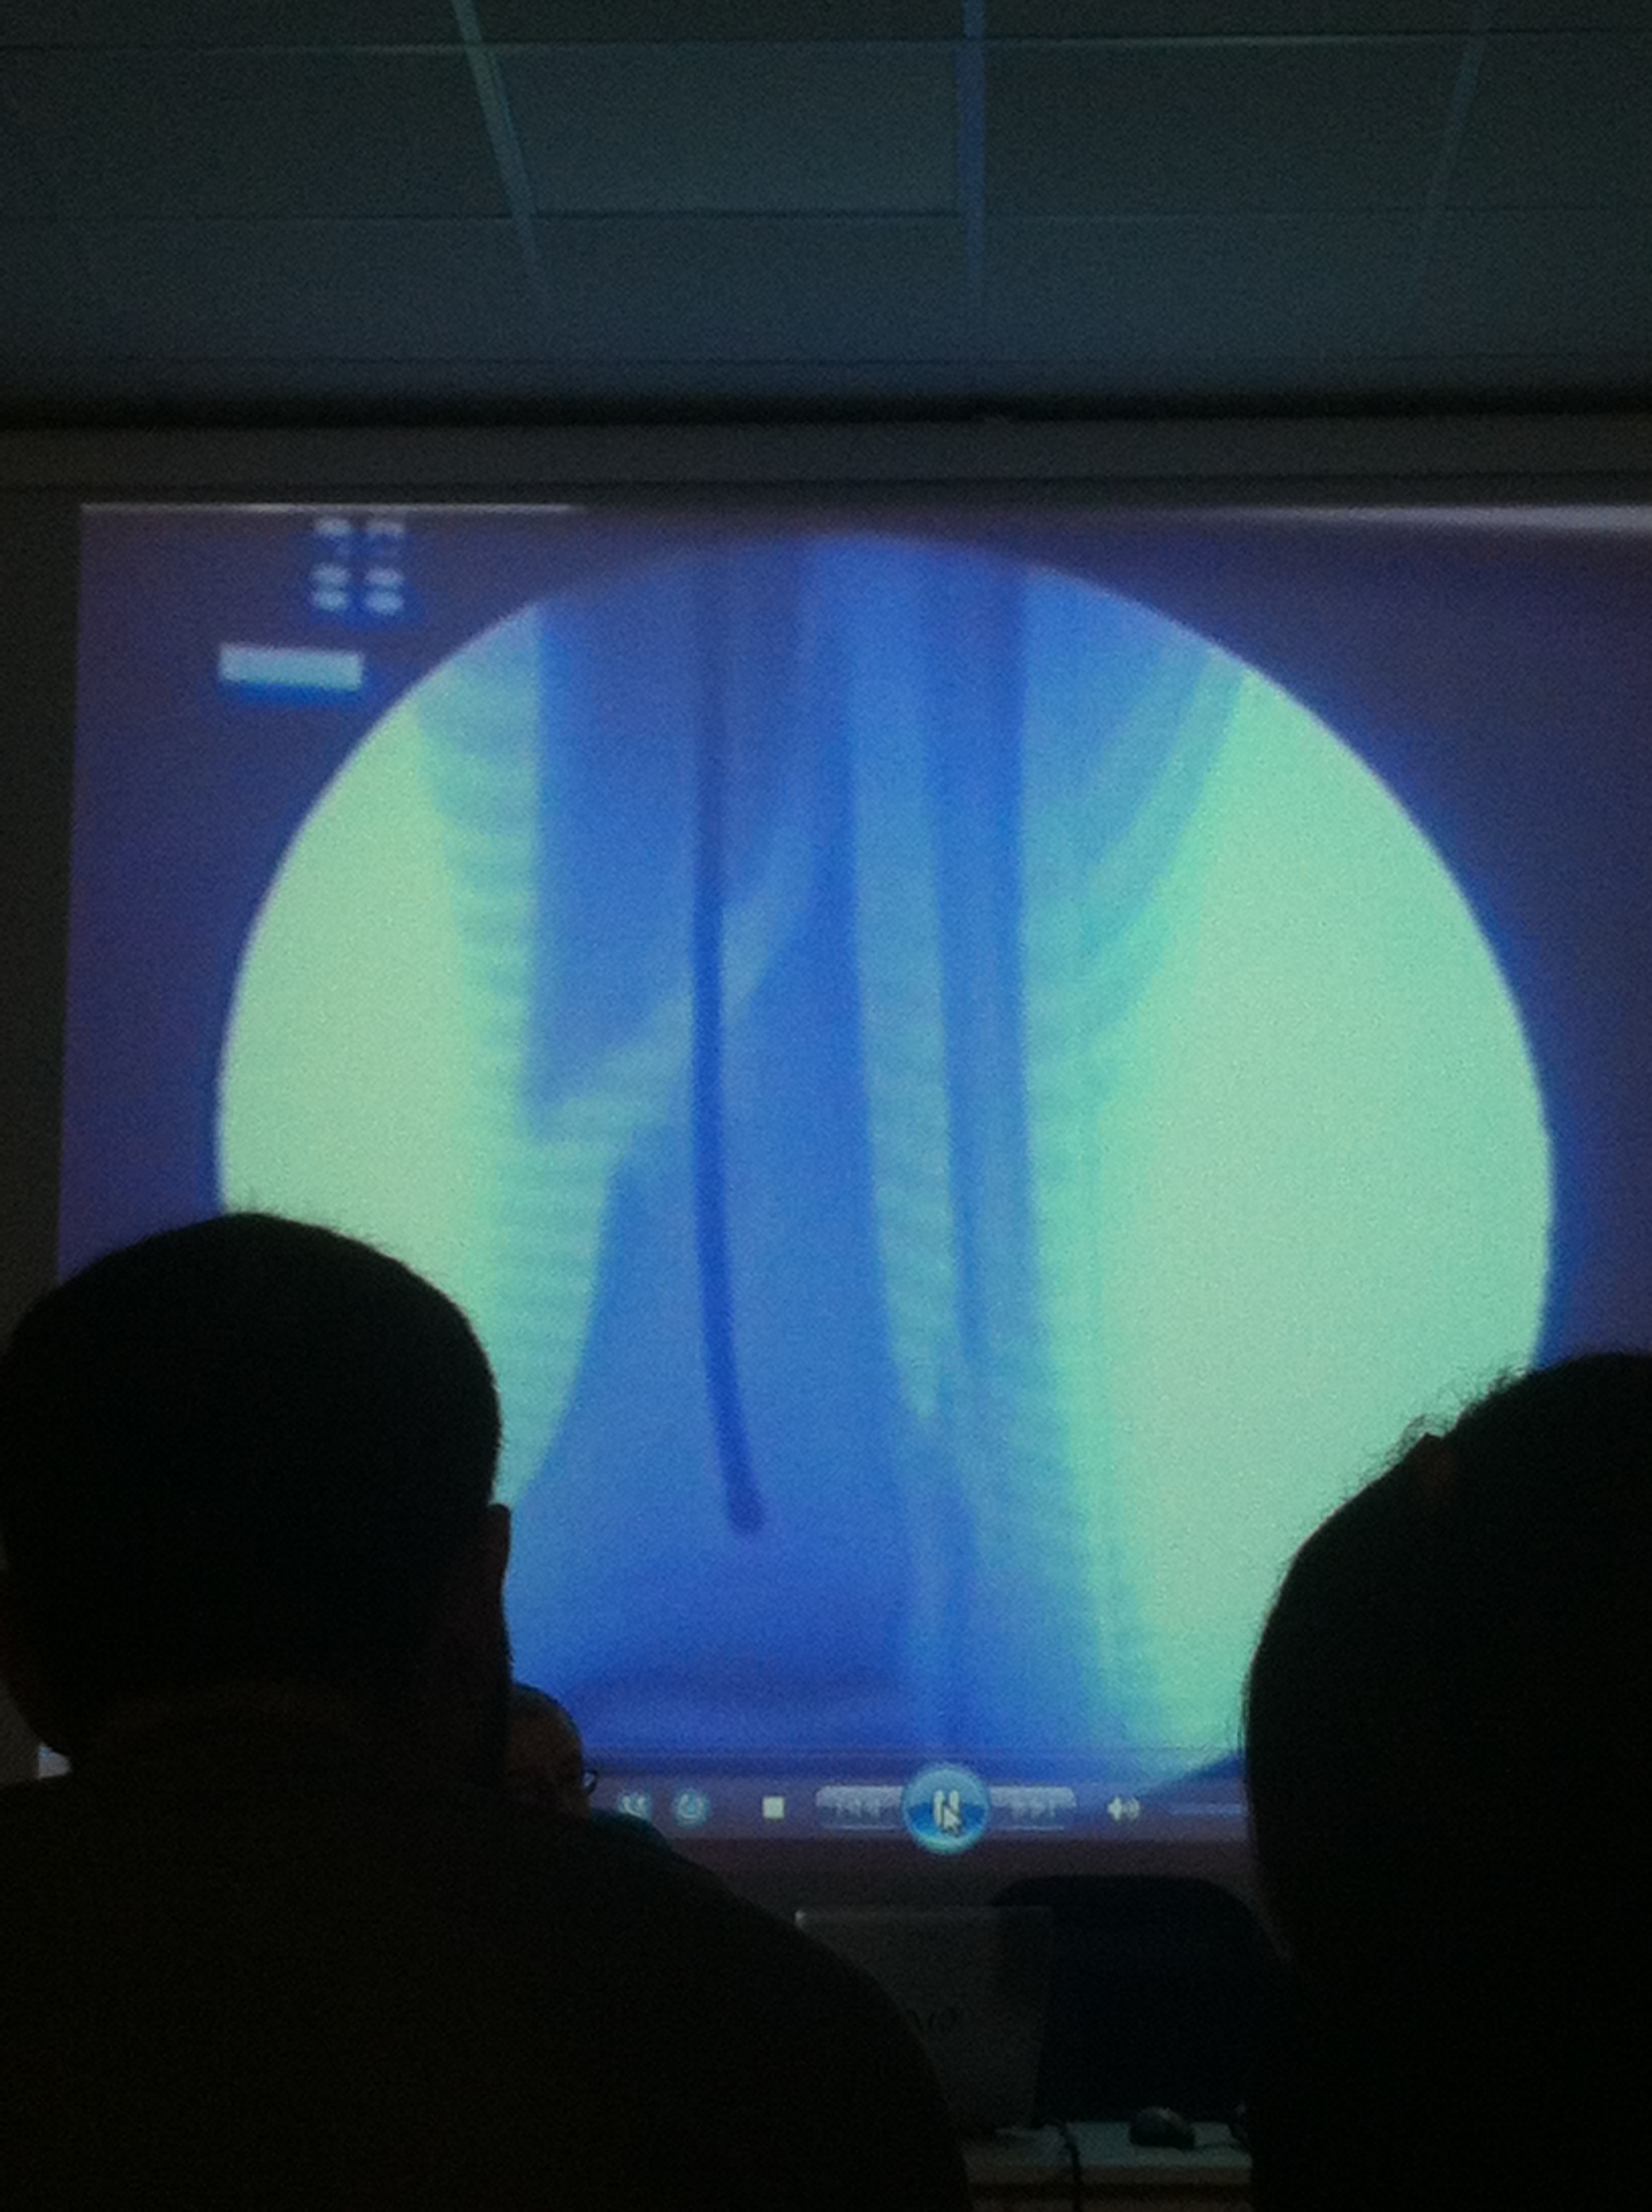
\includegraphics[width=0.3\textwidth]{001/image1.jpeg}
\end{figure}

Le fratture possono essere suddivise in:
\begin{itemize}
\item
  \emph{Traumatiche}
\item
  \emph{Patologiche, e ``da fragilità''}
\item
  \emph{Da stress (o da durata)}
\item
  \emph{Iatrogene (osteotomie)}
\end{itemize}



Nell'immagine: radiografia della gamba che mostra un segmento osseo discontinuo. Si tratta di una frattura del terzo distale della tibia e del terzo distale del perone.


\subsection{Diagnosi ( questa parte è stata ripresa e approfondita nella lezione del
08-03 )}

Per la diagnosi di frattura vanno sempre considerati più aspetti.

\subsubsection{Segni di probabilità}

\begin{itemize}
\item
  Atteggiamento: un paziente con un arto (o l'intero corpo) in posizione antalgica può far sospettare una frattura; ad esempio l'atteggiamento tipico delle fratture del collo del femore: l'arto è extra ruotato, addotto e accorciato
\item
Deformità grossolane, ad esempio la gamba in un senso e il piede nell'altro
\item
Lesioni cutanee e tumefazioni
\item
 Impotenza funzionale
\item
 Dolore
\end{itemize}

\subsubsection{Segni di certezza}

\begin{itemize}
\item
 Crepitio: la cauta mobilizzazione del segmento evoca il rumore delle superfici ossee a confronto
\item
 Motilità preternaturale
\end{itemize}

Per la \textbf{diagnosi definitiva} ci si avvale delle tecniche radiologiche: inizialmente radiografica, eventualmente TC o RM (se dovessero permanere dubbi o in caso si sospettino lesioni ai tessuti circostanti).

Nel momento in cui si ha un sospetto di frattura occorre procedere come di seguito:

\begin{itemize}
\item
  Immobilizzazione provvisoria sul luogo dell'incidente
\item
  Radiografia convenzionale (che permette la diagnosi di frattura).
N.B. La radiografia permette anche di definire e analizzare le caratteristiche di tale frattura
\item
  Trazione se necessario
\end{itemize}


\subsection{Trattamento}

Una volta fatta diagnosi di frattura inizia il processo di \textbf{riparazione della frattura}. \emph{Il trattamento delle frattura ha come scopo il recupero funzionale completo del segmento fratturato senza deformità residue o alterazioni significative della morfologia scheletrica e con il pieno recupero della funzione muscolare e articolare.}

Ci sono due aspetti da considerare e che garantiscono la guarigione di una frattura:

\begin{itemize}
\item
  \textbf{Riduzione della frattura}: si tratta del complesso di manovre messe in atto nel caso di frattura scomposta o fratture-lussazioni al fine di riposizionare i segmenti ossei nella corretta posizione anatomica. Tale manovra viene può essere eseguita dall'ortopedico manualmente ed è appunto detta manuale oppure essere eseguita chirurgicamente. A seguito di questo bisogna procedere con la stabilizzazione.

\item
  \textbf{Stabilizzazione} dei vari elementi della frattura. Si attua per mezzo di un apparecchio gessato o chirurgicamente attraverso l'utilizzo di diversi mezzi di sintesi in genere mezzi metallici tramite cui si fissa la frattura una volta che è stata ridotta. Tali mezzi di sintesi comprendono viti metalliche, placche associate a viti, chiodi endomidollari, fissatori esterni, fili metallici che passano attraverso la cute e bloccano la frattura.
\end{itemize}

In base alle modalità per cui si opta distinguiamo un \textbf{\emph{trattamento conservativo}} e uno \textbf{\emph{chirurgico (osteosintesi)}}


\paragraph{Trattamento conservativo}

Può essere così schematizzato:

\begin{itemize}
\item
  \emph{\textbf{Immobilizzazione} generalmente durante il trasporto in Pronto Soccorso, }
\item
  \emph{\textbf{Riduzione}: \textbf{manuale} oppure mediante \textbf{trazione progressiva}. In questo ultimo caso mediante applicazione ai capi ossei di un bendaggio adesivo (\textbf{trazione a cerotto}) oppure mediante un \textbf{filo transcheletrico} che permette di applicare fino a 14-15 Kg di peso.}
\item
  \emph{\textbf{Stabilizzazione} (o contenzione): tramite apparecchi gessati (classico), gessi funzionali interrotti laddove ci sono articolazioni (utili nel ginocchio) o gessi sintetici (che sono però poco plasmabili).}
\end{itemize}


\paragraph{Trattamento chirurgico (osteosintesi)}

Comporta l'esposizione del focolaio di frattura e la \textbf{riduzione} viene eseguita a cielo aperto.
Per la \textbf{stabilizzazione} dei frammenti si può eseguire.

\subparagraph{Fissazione interna}
Si applicano, tramite piccolo taglio, svariati mezzi di osteosintesi costituiti da fili, viti libere, placche e viti (Nell' immagine in alto a dx: viti libere e placca e viti).
  
\begin{figure}[!ht]
\centering
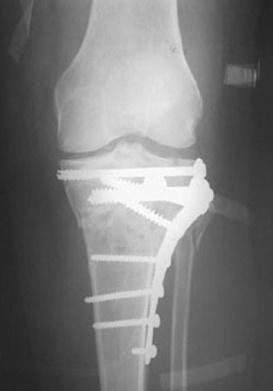
\includegraphics[width=0.25\textwidth]{001/image3.jpeg}
\end{figure}

\subparagraph{Fissazione esterna}
Si applicano viti o chiodi stabilizzati tra loro mediante un fissatore esterno che permette anche la riduzione della frattura. Viene preferita quando si ha un grosso rischio di infezione o in caso di fratture in determinate sedi: bacino, tibia e avambraccio (Nell'immagine: fissatore esterno).

\begin{figure}[!ht]
\centering
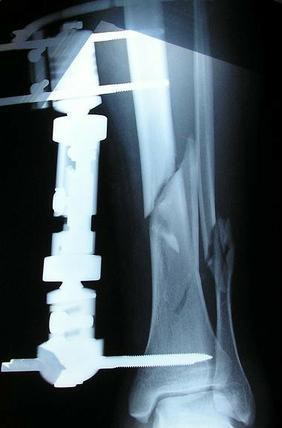
\includegraphics[width=0.25\textwidth]{001/image4.jpeg}
\end{figure}

\subparagraph{Sintesi endomidollari}
E' la più attuale! Sfrutta infibuli intra midollari che stabilizzano le fratture dall'interno. Questa metodica sfrutta la riparazione biologica col callo osseo periosteo diversamente dalla riparazione interna in cui si attua un'interruzione del processo ripartivo (Nell'immagine: chiodo Gamma).
  
\begin{figure}[!ht]
\centering
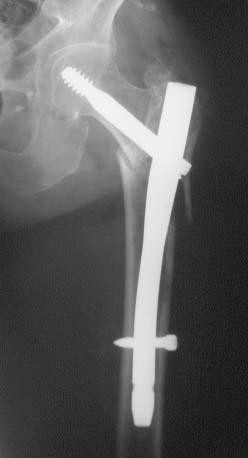
\includegraphics[width=0.25\textwidth]{001/image2.jpeg}
\end{figure}


In determinati casi le fratture non sono riparabili o meglio non conviene ripararle. Questo succede soprattutto negli anziani perché l'allettamento e la riabilitazione determinerebbero un crollo psicofisico ben peggiore della frattura stessa (sindrome da allettamento).

A questo punto il professore mostra un video di un intervento chirurgico di riduzione di una frattura e stabilizzazione chirurgica della stessa.
(Alcuni concetti precedenti vengono ripresi) Si tratta di una frattura del terzo distale della tibia. Viene mostrata la radiografia che conferma il sospetto diagnostico: si tratta di una frattura spiroide
scomposta (tipica frattura da torsione) in cui i due segmenti ossei non sono a contatto tra di loro. La frattura è stata trattata in sala operatoria sotto controllo endoscopico e per l'immobilizzazione la
scelta è stata quella della sintesi con chiodo endomidollare.

\begin{figure}[!ht]
\centering
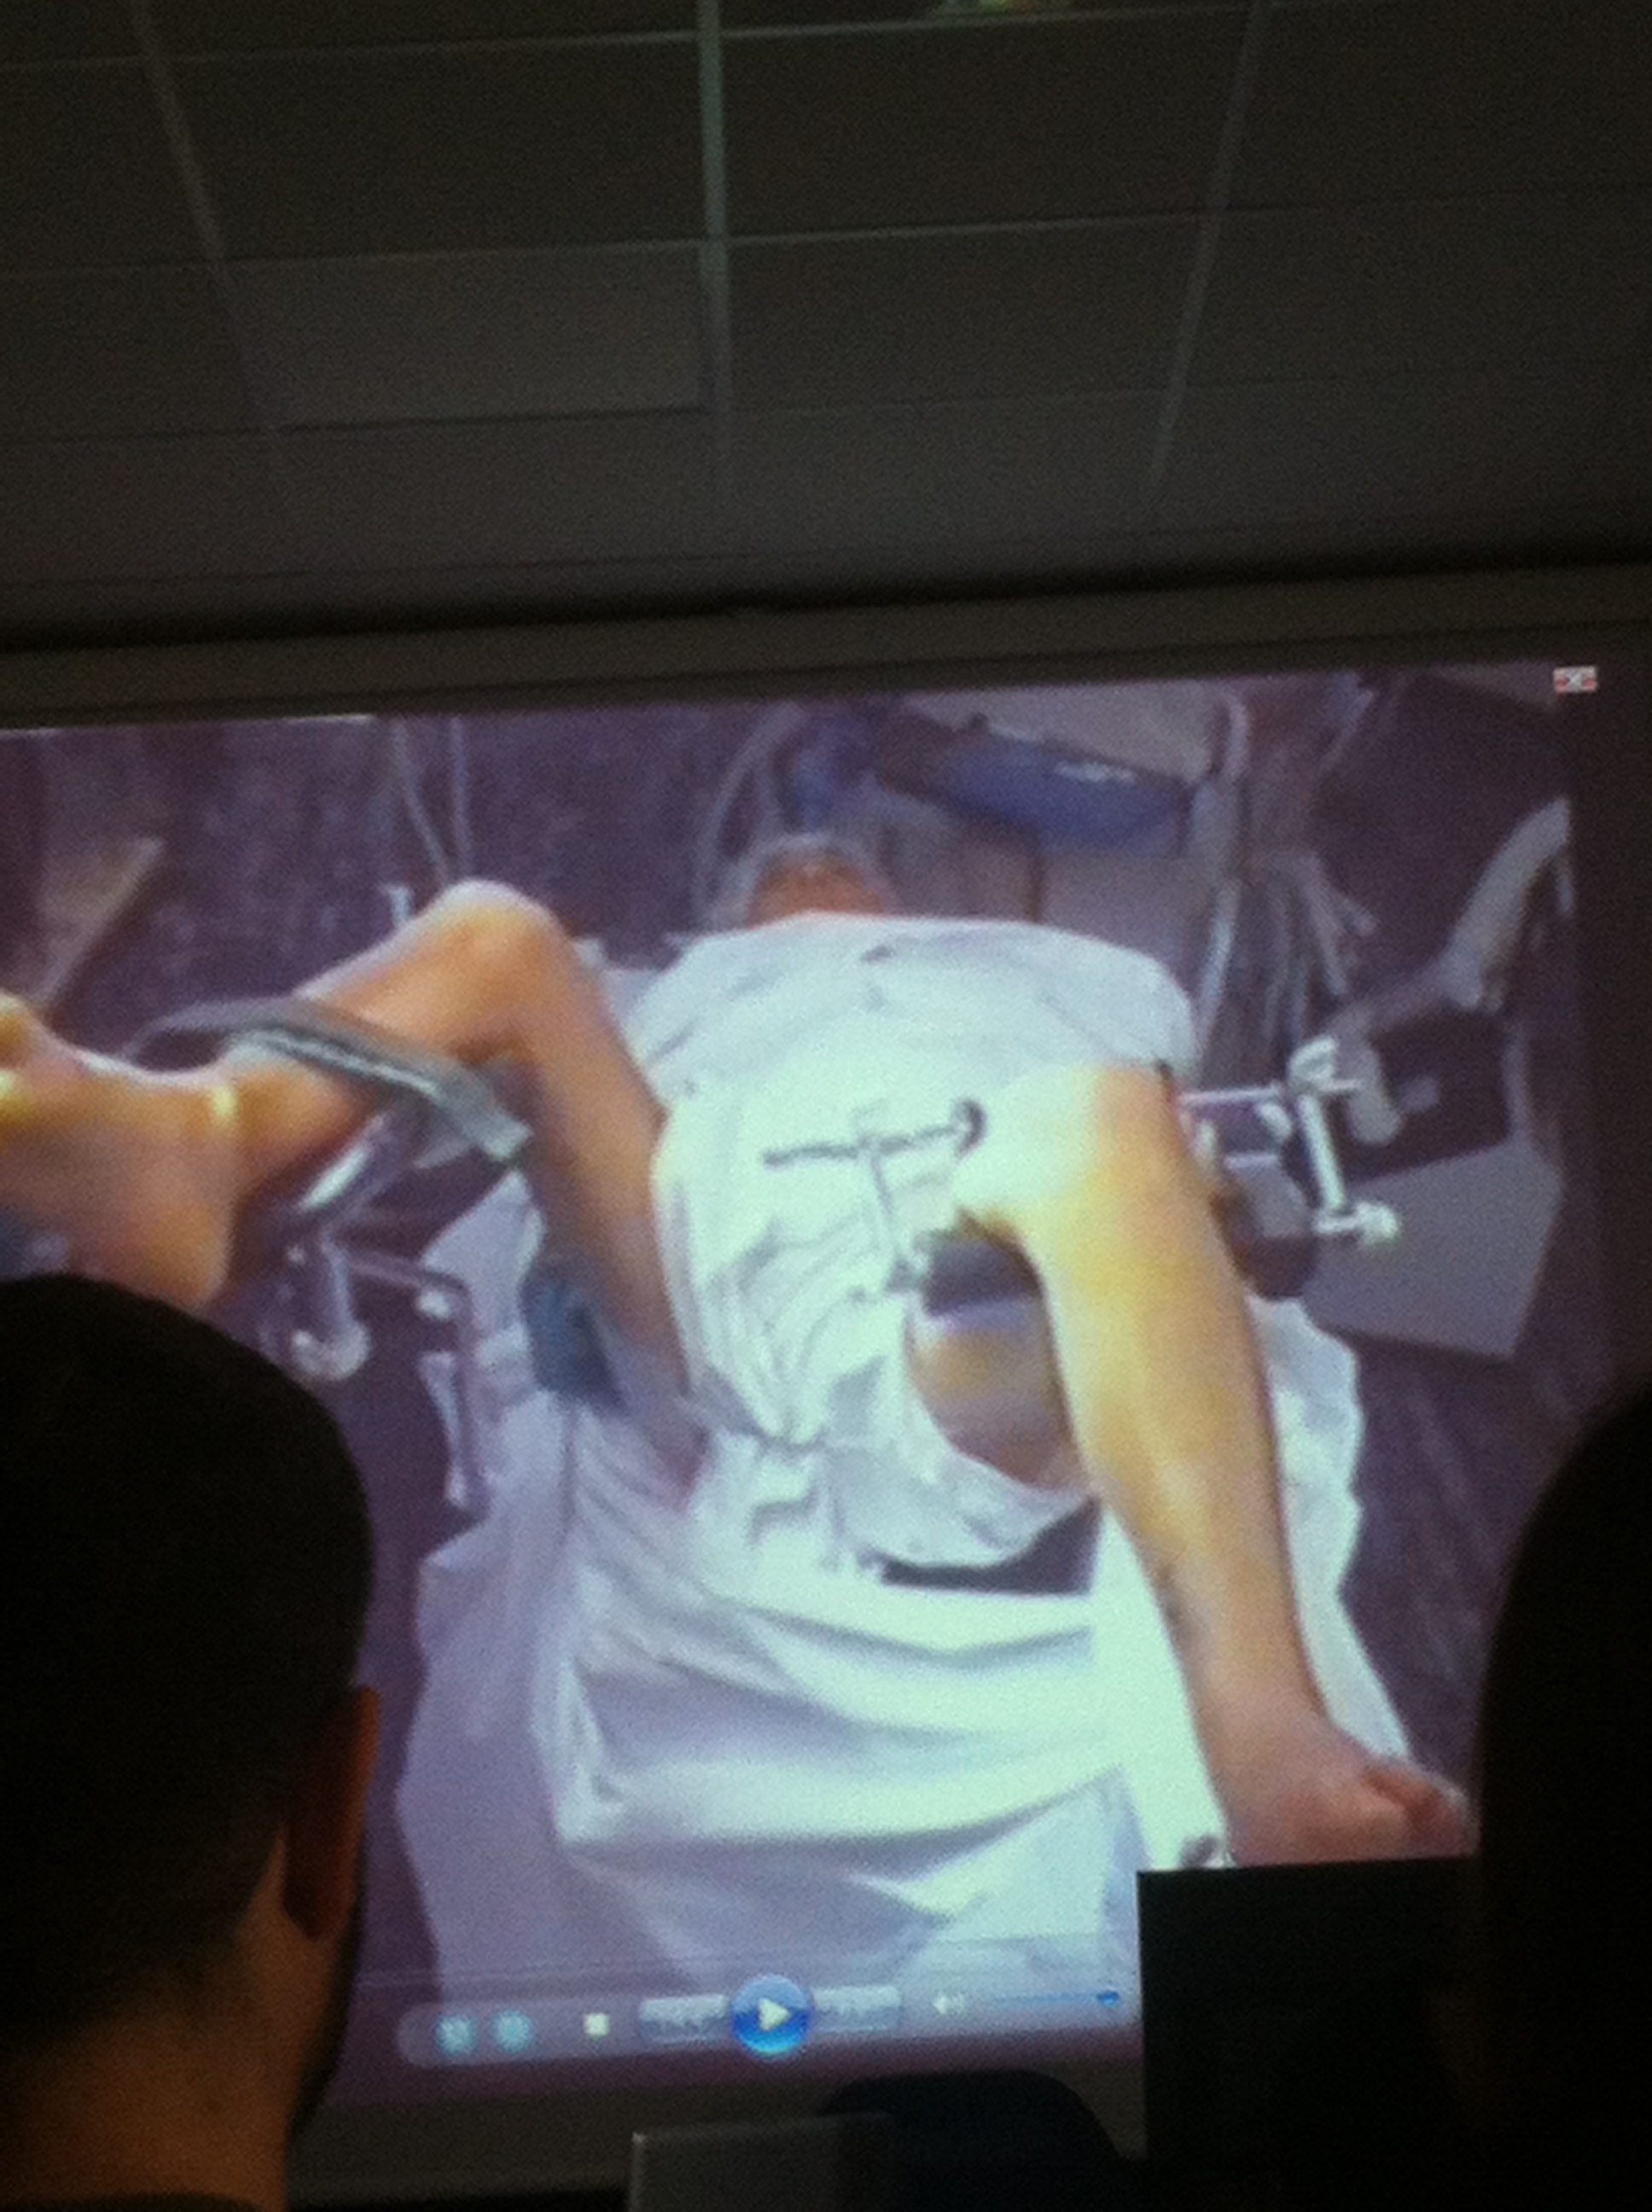
\includegraphics[width=0.3\textwidth]{001/image8.jpeg}
\end{figure}

La manovra di riduzione molto spesso viene eseguita sotto controllo dei raggi e si ricorre a posizioni particolari che facilitano la manovra stessa di riduzione e il posizionamento del chiodo (in questo caso il paziente è disteso sul lettino con le gambe sollevate). Molto spesso di fronte a una frattura delle ossa lunghe il paziente viene messo in \emph{trazione trans-scheletrica}: metodologia attuata per ridurre la
frattura e generalmente applicata in pronto soccorso in anestesia locale. Lo scopo di tale manovra è quello di \emph{trazionare progressivamente la frattura in vari segmenti corporei}: vengono progressivamente sgranati i frammenti della frattura e tesi i tessuti molli al fine di ridurre il gonfiore. Si tratta a tutti gli effetti di una parziale riduzione che verrà completata in seguito chirurgicamente. Ha il vantaggio di agevolare la fase chirurgica stessa. In questo caso è
stato posizionato il filo di trazione al calcagno e al letto vengono applicati pesi in kg che garantiscano la trazione.

Tali pesi devono essere pari al 5-10\% del peso corporeo per cui ad esempio per una frattura scomposta di femore in un soggetto di 70-80 kg si utilizzeranno pesi di 3,5/7 Kg. Importante ricordare i rischi legati
alla procedura stessa: un'eccessiva trazione può determinare eccessivo stiramento e parestesie o formicolio degli arti che devono essere necessariamente risolte.

A questo punto viene spiegata la procedura eseguita.. Attraverso proiezioni antero-posteriori e laterali il chirurgo controlla la fase di inserimento e procede alla riduzione della frattura. Questa manovra può
essere realizzata con l'ausilio di pinze o attraverso la cute previa incisione per raggiungere il focolaio della frattura. Nel video mostrato il chirurgo procede con incisione cutanea tramite la quale accede al
focolaio di frattura. A seguito della riduzione si procede con la \emph{stabilizzazione} che nel caso mostrato viene realizzata attraverso l'inserimento di un chiodo endomidollare che viene bloccato sopra e
sotto la frattura per dare stabilità. I chiodi sono cannulati, con buchi all'interno e necessitano dell'inserimento di un filo guida nel canale
midollare. Prima dell'inserimento del chiodo, si fresa il canale
midollare di uno o due mm in più del diametro del chiodo scelto, manovra
chiamata \textbf{ALESAGGIO DEL CANALE MIDOLLARE}.
\\\\
NB: Il chiodo a battuta viene posizionato solo se in tutte le proiezioni la frattura è riportata in posizione corretta! La punta del chiodo supera il focolaio di frattura e una volta posizionato con precisione verrà bloccato prossimalmente e distalmente con delle viti. Nel chiodo ci sono fori per le viti che posizionate perpendicolarmente vanno a bloccare il
chiodo sotto la frattura e in alto, sopra la stessa.

\begin{figure}[!ht]
\centering
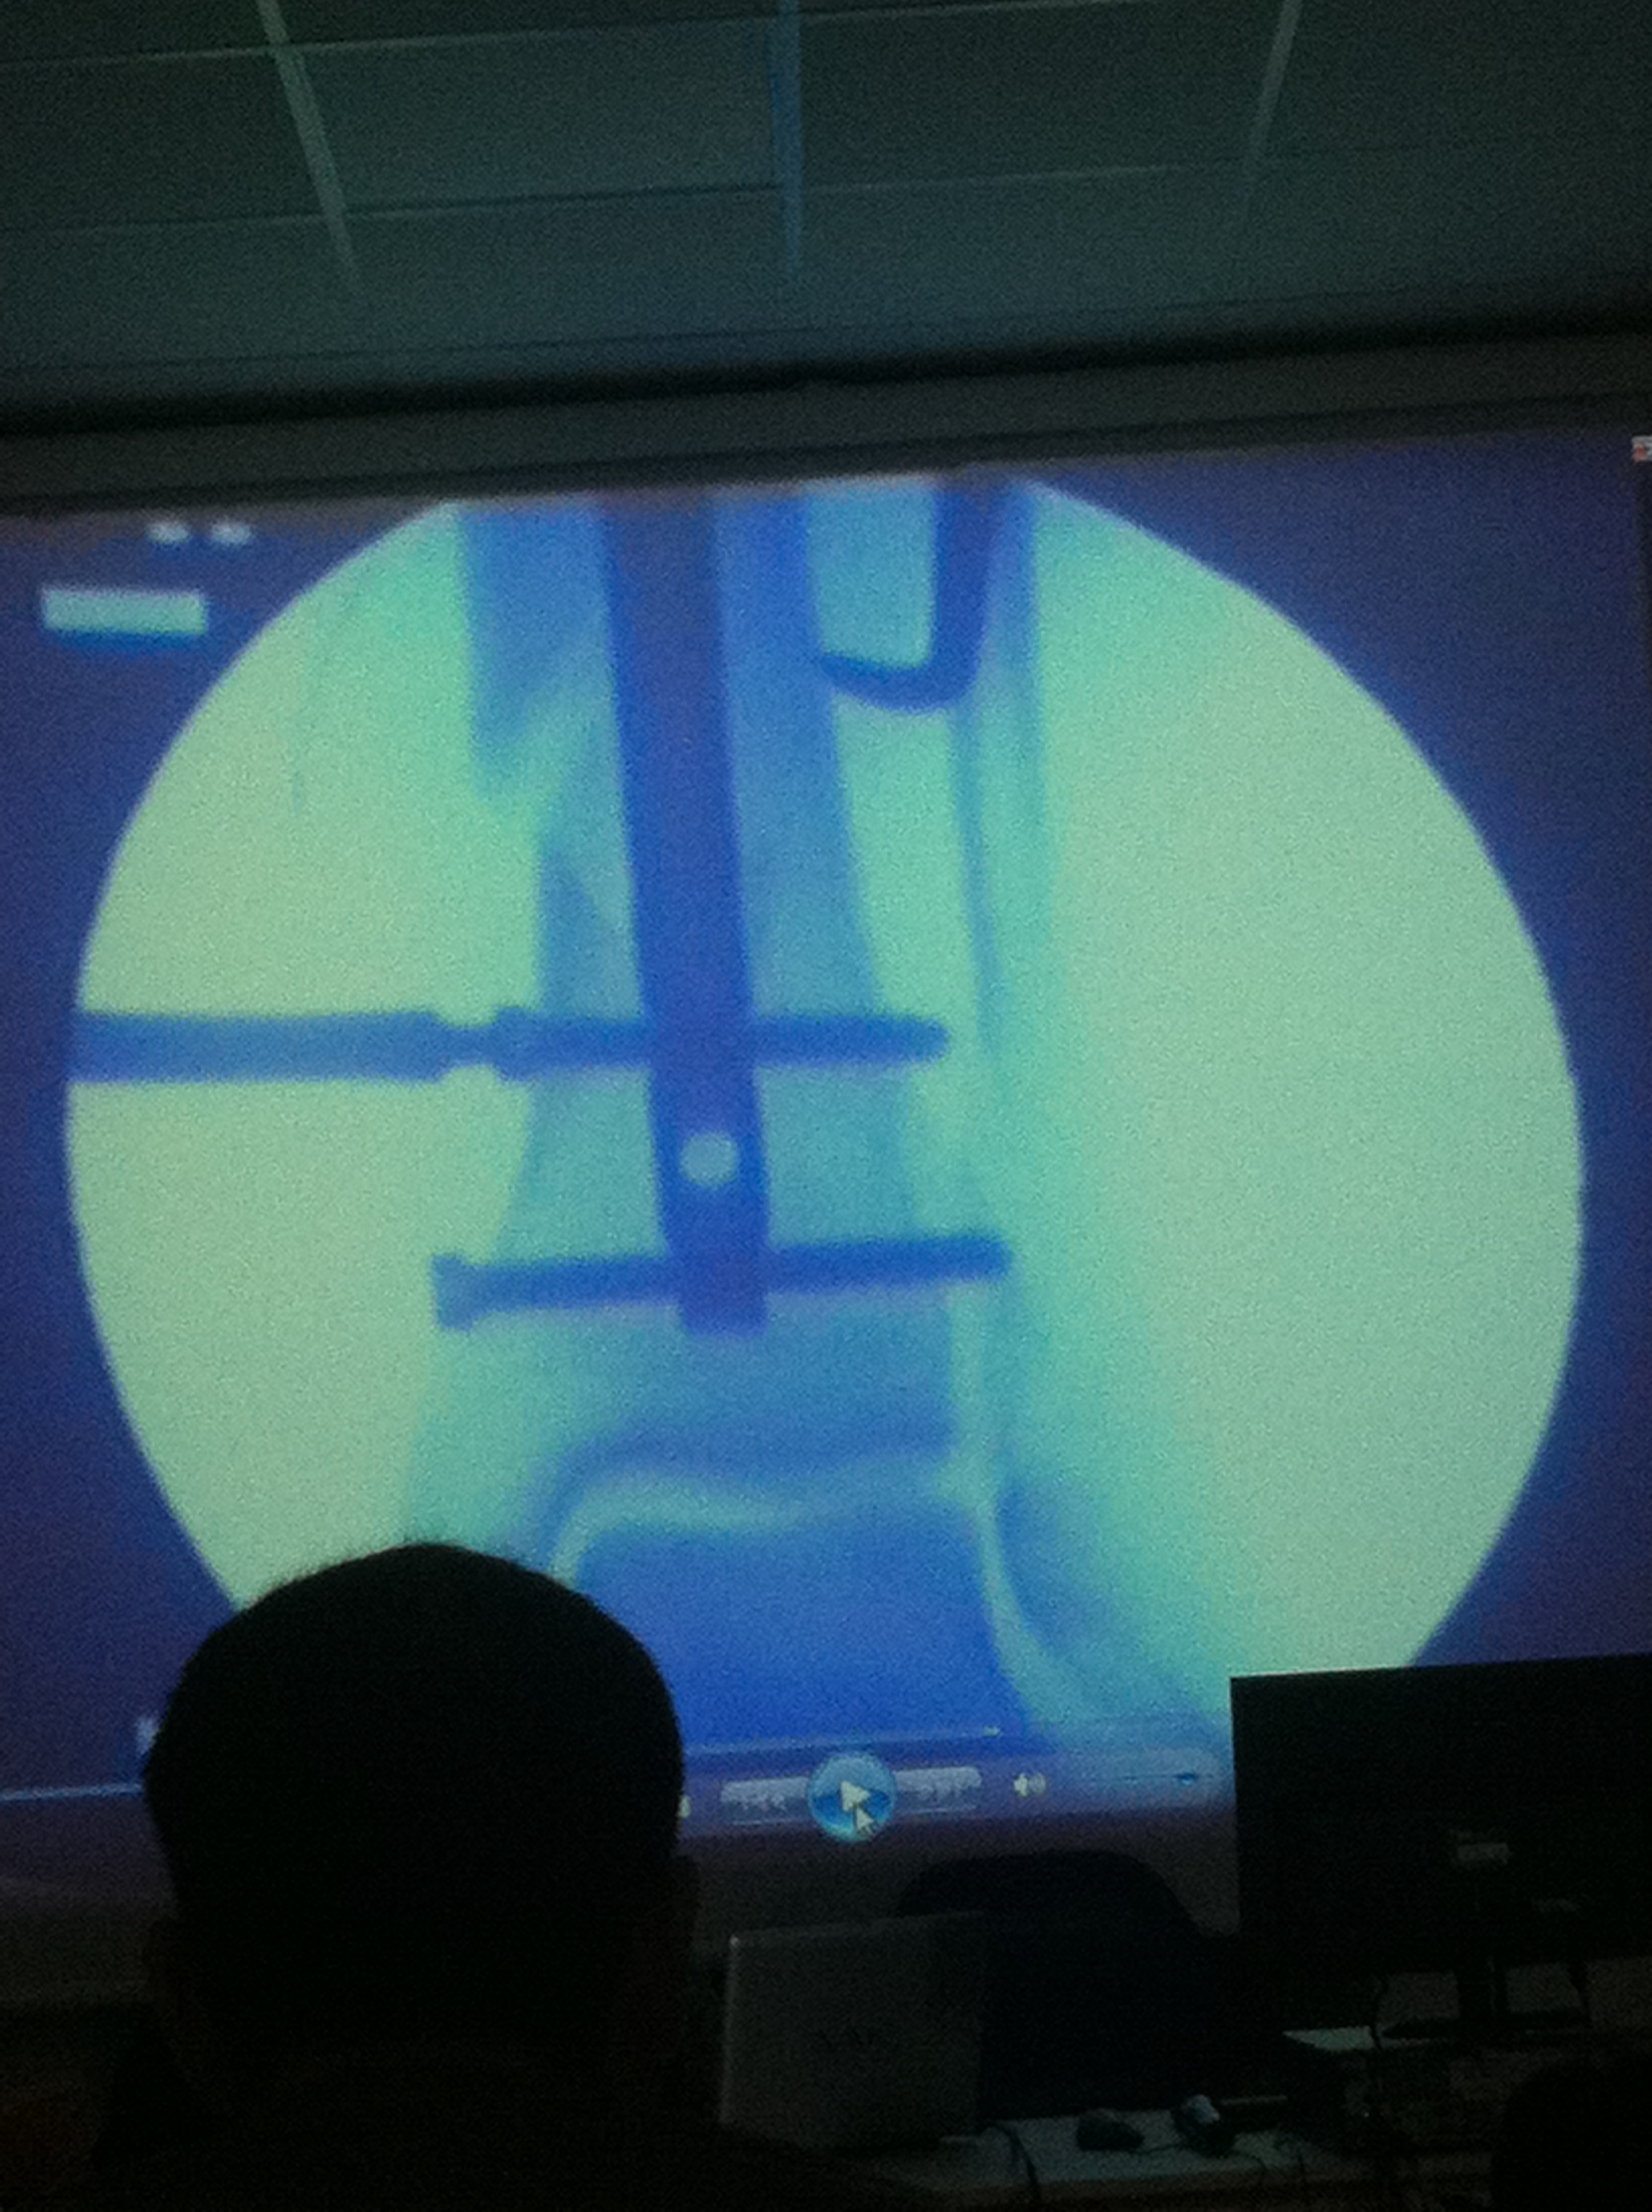
\includegraphics[width=0.3\textwidth]{001/image9.jpeg}
\end{figure}

PER RIASSUMERE:
\begin{itemize}
\item Diagnosi radiografica
\item Riduzione della frattura manuale o chirurgica (a cielo aperto con incisione o percutaneo con pinze)
\item Stabilizzazione della frattura: attraverso tutori, gesso, mezzi di sintesi inseriti chirurgicamente per favorire la guarigione.
\end{itemize}

La maggior parte delle fratture viene oggi trattata chirurgicamente, soprattutto se interessano le ossa lunghe. La chirurgia permette una riduzione migliore e una riabilitazione più rapida per cui minor incidenza di complicanze legate all'allettamento delle persone anziane e di complicanze locali come rigidità articolari. Il lavoro dell'ortopedico deve sempre andare di pari passo al lavoro del fisiatra/fisioterapista per ottenere il pieno recupero funzionale.

\newpage

\paragraph{\emph{Informazioni sul corso, tirocinio, modalità di svolgimento dell'esame:}}

\emph{Ortopedia e traumatologia: 3 cfu }

\emph{Medicina fisica e riabilitazione: 2 cfu }

\emph{TIROCINIO: Il tirocinio ha una durata di una settimana (Lun- Ven).
Sul sito è presente l'elenco delle settimane disponibili. Non più
disponibile reumatologia. Si viene suddivisi al mattino nelle varie
postazioni: ambulatorio traumi, pronto soccorso, medicina fisica e
riabilitazione.}

\emph{A tirocinio ogni giorno c'è un modulo in cui far apporre timbro e
firma del tutor, a fine settimana bisogna lasciare il libretto in
Segreteria (secondo piano Ortopedia, signora Giovanna). Ricordarsi di
presentare il libretto firmato all'esame!!}

\emph{In sala operatoria si può eccedere solo se interessati, è
necessario fare richiesta. C'è la possibilità di fare tirocinio a
Fidenza o Piacenza, comunicarlo per tempo al prof Coordinatore del corso
(prof. Pogliacomi).}

\emph{Se interessati alla materia si può frequentare il reparto.
Possibilmente iscriversi il prima possibile ai tirocini, in vicinanza
dell'esame. \emph{NB: Da sostenere entro l'anno accademico!} Le date dei
tirocini sono tutte sul sito, iscrizione online.}

\emph{ESAME: orale, iscrizione online e registrazione online. L'esame si
compone di 3 domande, riguardanti le materie del corso (una di
ortopedia, una di traumatologia, una di medicina fisica e
riabilitazione). Un prof può chiedere tutte e tre le domande o solo una:
è variabile! Il voto finale è costituito dalla media dei tre voti.
\emph{Tutte e tre le domande devono essere sufficienti per passare
l'esame}.}

\emph{I testi consigliati si trovano sul sito del corso.}

\documentclass[]{article}
\usepackage{lmodern}
\usepackage{amssymb,amsmath}
\usepackage{ifxetex,ifluatex}
\usepackage{fixltx2e} % provides \textsubscript
\ifnum 0\ifxetex 1\fi\ifluatex 1\fi=0 % if pdftex
  \usepackage[T1]{fontenc}
  \usepackage[utf8]{inputenc}
\else % if luatex or xelatex
  \ifxetex
    \usepackage{mathspec}
  \else
    \usepackage{fontspec}
  \fi
  \defaultfontfeatures{Ligatures=TeX,Scale=MatchLowercase}
\fi
% use upquote if available, for straight quotes in verbatim environments
\IfFileExists{upquote.sty}{\usepackage{upquote}}{}
% use microtype if available
\IfFileExists{microtype.sty}{%
\usepackage{microtype}
\UseMicrotypeSet[protrusion]{basicmath} % disable protrusion for tt fonts
}{}
\usepackage[unicode=true]{hyperref}
\hypersetup{
            pdfborder={0 0 0},
            breaklinks=true}
\urlstyle{same}  % don't use monospace font for urls
\usepackage{graphicx,grffile}
\makeatletter
\def\maxwidth{\ifdim\Gin@nat@width>\linewidth\linewidth\else\Gin@nat@width\fi}
\def\maxheight{\ifdim\Gin@nat@height>\textheight\textheight\else\Gin@nat@height\fi}
\makeatother
% Scale images if necessary, so that they will not overflow the page
% margins by default, and it is still possible to overwrite the defaults
% using explicit options in \includegraphics[width, height, ...]{}
\setkeys{Gin}{width=\maxwidth,height=\maxheight,keepaspectratio}
\IfFileExists{parskip.sty}{%
\usepackage{parskip}
}{% else
\setlength{\parindent}{0pt}
\setlength{\parskip}{6pt plus 2pt minus 1pt}
}
\setlength{\emergencystretch}{3em}  % prevent overfull lines
\providecommand{\tightlist}{%
  \setlength{\itemsep}{0pt}\setlength{\parskip}{0pt}}
\setcounter{secnumdepth}{0}
% Redefines (sub)paragraphs to behave more like sections
\ifx\paragraph\undefined\else
\let\oldparagraph\paragraph
\renewcommand{\paragraph}[1]{\oldparagraph{#1}\mbox{}}
\fi
\ifx\subparagraph\undefined\else
\let\oldsubparagraph\subparagraph
\renewcommand{\subparagraph}[1]{\oldsubparagraph{#1}\mbox{}}
\fi

% set default figure placement to htbp
\makeatletter
\def\fps@figure{htbp}
\makeatother


\date{}

\begin{document}

\emph{Le fratture}

\emph{Introduzione}

Le fratture sono definite come delle \emph{soluzioni di continuità di un
segmento osseo}.

Ogni segmento osseo ha una sua resistenza: per generare una frattura
quindi l'entità del trauma deve superare i limiti di elasticità e di
resistenza del segmento osseo colpito.

Di fronte ad una frattura (ad esempio di un osso lungo come il femore)
si possono riconoscere:

\begin{itemize}
\item
  \textbf{Focolaio di frattura:} corrisponde alla sede anatomica della
  frattura
\item
  \textbf{Rima della frattura:} rappresenta l'andamento della linea di
  demarcazione fra due o più segmenti di osso fratturato
\item
  \textbf{Monconi della frattura:} segmenti principali dell'osso
  fratturato
\end{itemize}

\begin{quote}
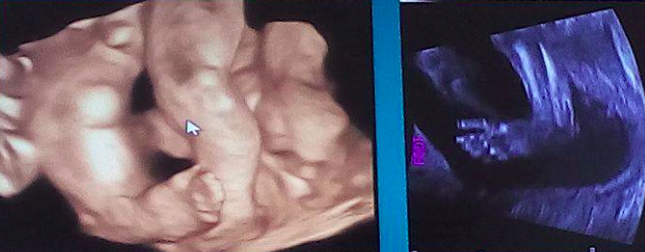
\includegraphics[width=6.64583in,height=4.19792in]{media/image1.png}

\emph{Classificazione}
\end{quote}

Le fratture possono essere classificate secondo diversi criteri.

\begin{quote}
\textbf{\emph{I.CLASSIFICAZIONE EZIOLOGIA}} (è la classificazione più
utilizzata) Dal punto di vista eziologico distinguiamo:

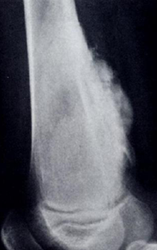
\includegraphics[width=2.67708in,height=1.95833in]{media/image2.png}
\end{quote}

\begin{itemize}
\item
  \textbf{Fratture traumatiche}: sono le fratture più frequenti e si
  verificano quando \emph{un \textbf{unico trauma efficiente} causa
  l'interruzione di un osso sano e strutturalmente normale.} Ad esempio
  se un motociclista urta contro un palo con conseguente frattura di
  tibia e perone allora definiremo quella come una frattura traumatica
  legata al trauma diretto della gamba contro il palo.
\item
  \textbf{Fratture da durata o da stress}: conseguenti \emph{a ripetuti
  \textbf{microtraumi non efficienti} che agiscono nel tempo su un osso
  sano}. Il cedimento strutturale è \emph{per sovraccarichi funzionali
  che superano i limiti di resistenza meccanica dell'osso stesso. Sono
  per definizione stessa delle fratture incomplete! Tuttavia se il
  meccanismo lesivo non viene interrotto, evolvono in vere e proprie
  fratture complete che coinvolgono principalmente gli arti inferiore
  dal momento che questi sono esposti a carichi di lavoro maggiori.}
  Possiamo prendere in considerazione diverse situazioni come ad esempio
  quella di un maratoneta che si allena costantemente e partecipa a 3/4
  maratone l'anno, può andare incontro ad una frattura da stress del
  metatarso. Altra frattura da stress comune è quella dei metacarpi nei
  pugili o del collo del femore o del piatto tibiale nei Marines (c'è
  molta letteratura al riguardo).
\item
  \textbf{Fratture patologiche}. Si tratta di una tipologia la cui
  incidenza è progressivamente aumentata negli ultimi anni. Si
  instaurano su un \emph{``osso patologico}'' cioè un osso che risulta
  essere più debole del normale e meccanicamente insufficiente. Molto
  spesso non è nemmeno presente l'evento traumatico o talvolta è un
  trauma inefficace. Le cause che portano ad un indebolimento dell'osso
  possono essere varie e ne vediamo alcune:
\end{itemize}

\begin{itemize}
\item
  \emph{Osteoporosi} ad esempio una persona anziana che si alza dalla
  sedia e accusa poi dolore alla schiena, può riportare una frattura dei
  corpi vertebrali su base osteoporotica. \emph{L'osteoporosi è definita
  come una riduzione della massa ossea con rarefazione delle trabecole
  nell'osso spongioso e assottigliamento della corticale che comporta un
  aumentato rischio di fratture. Va sottolineato che nell'osteoporosi la
  massa ossea è quantitativamente ridotta, ma qualitativamente normale
  perciò possono verificarsi fratture per traumi molto modesti come ad
  esempio al collo del femore o alle vertebre e nella maggior parte dei
  casi sono conseguenti a traumi multipli piuttosto che ad un unico
  trauma evidente.}
\end{itemize}

\begin{quote}
\textbf{N.B.:} Non abbiamo una definizione univoca per le fratture da
osteoporosi. Sul libro dice chiaramente che non sono classificabili come
fratture patologiche, ma nella lezione sulle fratture del collo del
femore (sulla vecchia dispensa Sigfied) il prof Ceccarelli le inserisce
tra le fratture patologiche ``border-line''. Durante questa lezione
(tenuta dal prof. Vaienti) sono riportate come esempio di fratture
patologiche e chiesti chiarimenti al prof., questi ribadisce che loro le
considerano come patologiche!
\end{quote}

\begin{itemize}
\item
  \emph{Malattie congenite} come ad esempio l'osteogenesi imperfetta
  (OI). \emph{Detta anche malattia delle ossa di vetro o malattie delle
  sclere blu, l'OI è una patologia che colpisce gli individui di sesso
  maschile principalmente ed è dovuta ad anomalie nella sintesi del
  collagene di tipo I con problemi a carico dello scheletro, delle
  articolazione, degli occhi (sclere blu), delle orecchie, della cute e
  dei denti. Può essere a penetranza più o meno completa e,
  conseguentemente, ad espressione clinica più o meno grave: oggi se ne
  conoscono sette tipologie a gravità diversa.}
\item
  \emph{Tumori:} sia tumori primitivi alle ossa come cisti ossee o
  tumori maligni primitivi sia metastasi di tumori in altre sedi tra cui
  più frequentemente tumore della mammella, del polmone, della prostata
  e dell'utero. \emph{Questi possono colpire tanto i bambini quanto gli
  adulti però nei bambini sono generalmente più benigni.}
\item
  \emph{Infezioni} come nel caso dell'osteomielite
\end{itemize}

N.B.Delle cause riportate ricordare che l'osteogenesi imperfetta è la
causa più ricorrente tra i bambini mentre l'osteoporosi tra gli anziani.
Le lesioni osteolitiche di natura neoplastica benigne o maligne,
primitive o secondarie riguardano principalmente gli adulti e anziano,
ma a volte anche i bambini

\begin{itemize}
\item
  \textbf{Fratture iatrogene} \textbf{o osteotomie chirurgiche}:
  interruzioni del tessuto osseo \emph{realizzate dal chirurgo a fini
  terapeutici quindi per correggere una deformità.} Possono essere
  realizzate manualmente o più frequentemente mediante l'utilizzo di
  strumenti chirurgici (seghe, fili, scalpelli, osteotomi). Ad esempio
  nel caso di ginocchio varo (è il cosiddetto ginocchio a parentesi:
  l'opposto del ginocchio a X o ginocchio valgo) viene trattato
  schematicamente così: con lo scalpello si effettua la frattura
  iatrogena quindi si corregge la deformità ed infine si blocca il tutto
  con una piastra e delle viti. Per l'osteotomia dell'anca finalizzata a
  correggere un'anca displasica (es. osteotomia di Salter, osteotomia di
  Chiari) si procede come di seguito: si frattura l'acetabolo, si
  riorienta nella posizione corretta e poi si blocca con delle viti.
  \emph{Infine l'osteotomia è eseguita anche per correggere eterometrie
  degli arti.} \emph{La calloclasia invece è l'interruzione chirurgica
  di un callo osseo che si effettua quando la frattura si sta riparando
  in modo inadeguato}
\end{itemize}

\begin{quote}
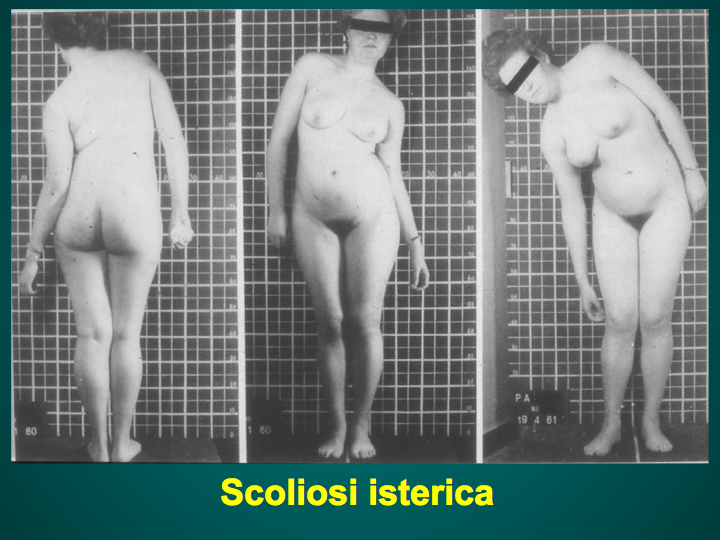
\includegraphics[width=3.88542in,height=2.81250in]{media/image3.png}
\end{quote}

\textbf{II. CLASSIFICAZIONE IN BASE AL TIPO DI TRAUMA}

\begin{itemize}
\item
  \textbf{Frattura per trauma diretto:} il trauma agisce nel punto
  stesso in cui si manista la frattura. Ad esempio un soggetto che
  riceva un calcio al terzo medio della tibia con conseguente frattura
  dell'osso in quel punto. \emph{Distingueremo in questo caso:}
\end{itemize}

\begin{itemize}
\item
  \emph{Fratture da urto}
\item
  \emph{Fratture da schiacciamento}
\item
  \emph{Fratture penetranti (o da arma da fuoco)}
\end{itemize}

\begin{itemize}
\item
  \textbf{Frattura per trauma indiretto:} in questo caso il trauma causa
  una frattura a distanza rispetto al punto di applicazione del trauma
  stesso. Ad esempio chi cade sulla mano, ma riporta una frattura del
  gomito. \emph{{[}La vecchia dispensa Sigfied suddivide ulteriormente
  la fratture indirette in fratture per torsione, per flessione, per
  compressione, per trazione e per azione combinata. Nella lezione il
  prof non riporta tale sub classificazione e procede con la
  classificazione in base al meccanismo lesivo che coincide con tale sub
  classificazione riportata nella vecchia dispensa{]}}
\end{itemize}

.

\textbf{III. CLASSIFICAZIONE IN BASE AL MECCANISMO LESIVO}

\begin{itemize}
\item
  \textbf{Fratture da flessione:} il trauma determina una modifica della
  normale curvatura dell'osso fino alla rottura. \emph{Ad esempio le
  ginnaste che flettono troppo l'ulna.}
\item
  \textbf{Fratture da torsione:} in questo caso il trauma è di tipo
  torcente rispetto all'asse osso. \emph{Ad esempio se metto il piede
  tra il marciapiede e un altro ostacolo, il piedi si incastrerà e cadrò
  in avanti: si produce una rima di frattura spiroide.}
\item
  \textbf{Fratture da compressione o da schiacciamento:} \emph{l'esempio
  tipico è a livello dell'osso spongioso vertebrale}
\item
  \textbf{Fratture da strappamento:} in questo caso la trazione di un
  legamento o di un tendine causa il distacco dell'osso che ivi si
  inserisce\emph{.} Ad esempio a volte il legamento rotuleo ``strappa
  l'osso a livello della sua inserzione sulla tuberosità tibiale
  anteriore
\item
  \emph{\textbf{Fratture per azione combinata}}
\end{itemize}

\textbf{IV. CLASSIFICAZIONE IN BASE AL DECORSO DELLA RIMA}

\begin{itemize}
\item
  \textbf{Fratture trasversali:} la rima è ad \emph{angolo retto}
  rispetto all'asse longitudinale dell'osso
\item
  \textbf{Fratture oblique:} la rima forma un \emph{angolo minore di
  90°} rispetto all'asse longitudinale
\item
  \textbf{Fratture spiroidi:} la rima compie un \emph{decorso a spirale}
  rispetto al segmento osseo
\item
  \textbf{Fratture longitudinali:} la rima è \emph{parallela} all'asse
  longitudinale dell'osso
\end{itemize}

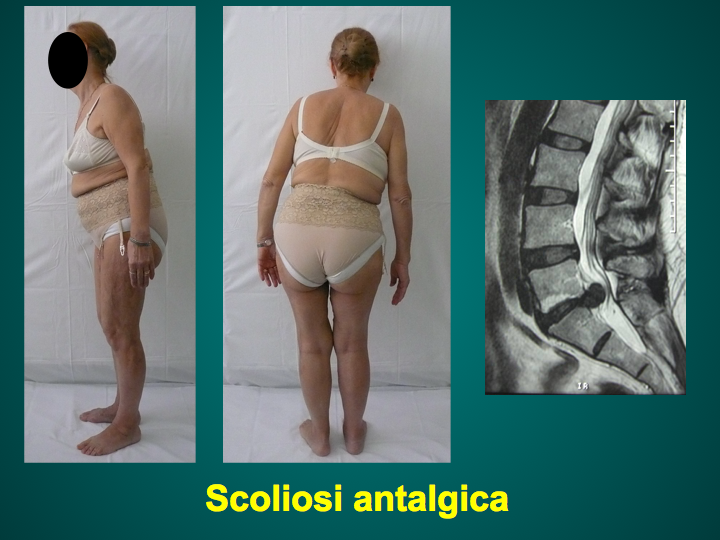
\includegraphics[width=3.34375in,height=2.00000in]{media/image4.png}
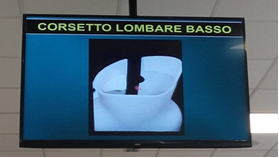
\includegraphics[width=3.65625in,height=2.78125in]{media/image5.png}

\begin{quote}
\textbf{V. CLASSIFICAZIONE PER SPOSTAMENTO DEI MONCONI}
\end{quote}

\begin{itemize}
\item
  \textbf{Fratture composte:} i frammenti \emph{conservano} la loro
  posizione e rapporti anatomici \emph{così da non modificare la normale
  configurazione dell'osso.}
\item
  \textbf{Fratture scomposte:} i frammenti \emph{non conservano} la loro
  posizione anatomica \emph{e la forma del segmento scheletrico appare
  alterata dallo spostamento dei frammenti stessi. Per la diafisi delle
  ossa lunghe si descrivono 4 tipi di scomposizione}
\end{itemize}

\begin{itemize}
\item
  \emph{Longitudinale:} i monconi si sovrappongono in lunghezza l'uno
  sull'altro
\item
  \emph{Angolare:} i monconi si angolano l'uno rispetto all'altro
\item
  \emph{Laterale:} i monconi non si sovrappongono, ma sono spostati
  lateralmente l'uno rispetto all'altro
\item
  \emph{Rotatorio:} i monconi ruotano l'uno sull'altro
\end{itemize}

\begin{itemize}
\item
  \textbf{Fratture scomposte e ingranate:} i monconi si ingranano l'uno
  sull'altro. Generalmente sono dovute a traumi da compressione. Una
  frattura scomposta ed ingranata dei corpi vertebrali, si riconosce
  all'RX perché normalmente il corpo vertebrale appare di forma
  rettangolare mentre in caso di frattura ingranata il rettangolo
  scompare e si vede una cuneizzazione perché la parte anteriore si
  schiaccia rispetto a quella posteriore
\end{itemize}

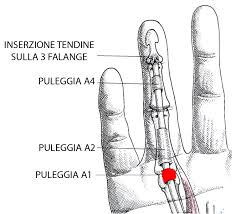
\includegraphics[width=6.03125in,height=3.62500in]{media/image6.png}

\textbf{VI. CLASSIFICAZIONE PER NUMERO DI FRAMMENTI}

\begin{itemize}
\item
  \textbf{Fratture unifocali:} una rima di frattura e due monconi
\item
  \textbf{Fratture bifocali:} due focolai di frattura posti a livelli
  diversi e tre monconi
\item
  \textbf{Fratture plurifocali o pluriframmentarie:} tanti focolai di
  frattura e tanti monconi.
\end{itemize}

\textbf{VII. CLASSIFICAZIONE PER SEDE SCHELETRICE (per ossa lunghe)}

\begin{itemize}
\item
  \textbf{Fratture diafisarie} (la diafisi è la parte centrale di un
  osso lungo)
\item
  \textbf{Fratture epifisarie} (l'epifisi è la parte articolare distale
  di un osso lungo)
\item
  \textbf{Fratture metafisarie} (la metafisi è a metà tra epifisi e
  diafisi)
\end{itemize}

\textbf{VIII. CLASSIFICAZIONE PER ALTRA SEDE (no sede scheletrica!) }

È la classificazione più comunemente riportata nei referti:

\begin{itemize}
\item
  \textbf{Frattura articolare:} \emph{la rima di frattura intacca la
  cartilagine articolare}. Caratterizzata da una prognosi peggiore
  legata alla maggiore frequenza di insorgenza di artrosi post-
  traumatica; per scongiurare tale evoluzione si cerca di ripristinare
  un piano cartilagineo il più normale possibile tuttavia molto spesso
  la cartilagine è troppo rovinata oppure risulta impossibile rimetterla
  a posto quindi si lasciano degli scalini di incongruenza.
\item
  \textbf{Frattura extra-articolare:} la rima di frattura non arriva a
  livello della cartilagine articolare e questo generalmente si associa
  ad una prognosi migliore perché non c'è rischio di artrosi
  post-traumatica. \emph{Queste sono ulteriormente suddivise in:}
\end{itemize}

\begin{itemize}
\item
  \emph{Intra-capsulari: sono generalmente piuttosto gravi perché spesso
  vanno incontro a devascolarizzazione e il danno vascolare limita la
  capacità di creare un callo osseo}
\item
  \emph{Extra- capsulari}
\end{itemize}

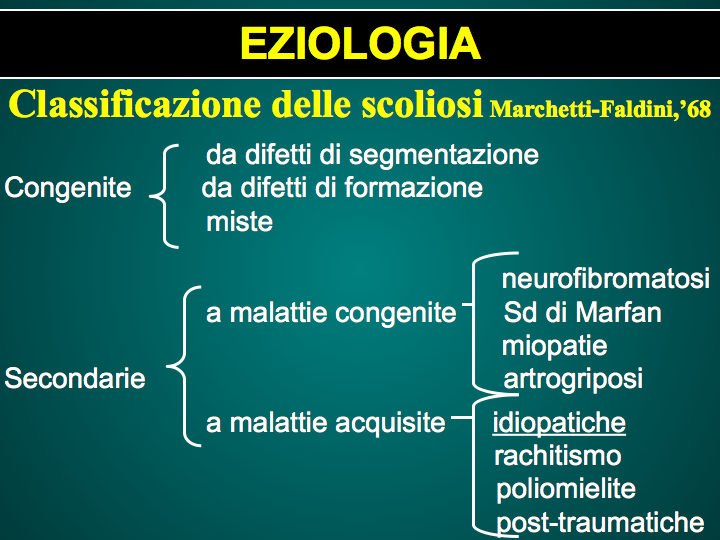
\includegraphics[width=5.58333in,height=4.07292in]{media/image7.png}

\textbf{IX. CLASSIFICAZIONE PER ENTITA' DEL DANNO}

\begin{itemize}
\item
  \textbf{Fratture complete:} interessano \emph{tutta la circonferenza}
  dell'osso
\item
  \textbf{Fratture incomplete:} \emph{non} interessano tutta la
  circonferenza. Possono essere a loro volta ulteriormente suddivise in:
\end{itemize}

\begin{itemize}
\item
  Fratture per infrazione
\item
  Fratture ``a legno verde'': questa espressione viene generalmente
  utilizzata quando si è di fronte ad una frattura in un bambino poiché
  in questo caso le loro ossa lunghe sono più plastiche rispetto a
  quelle di un adulto e quindi sono esposte ad un minor rischio di
  frattura. In questo caso avremo uno sfibramento o una piegatura, ma
  non una rottura dell'osso da cui il paragone con il legno verde che ha
  bisogno di una stimolazione più forte per spezzarsi rispetto ad un
  legno secco.
\end{itemize}

\begin{quote}
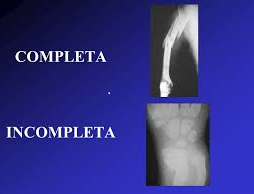
\includegraphics[width=2.64583in,height=2.02083in]{media/image8.png}
\end{quote}

\textbf{X. CLASSIFICAZIONE IN BASE ALL'INTEGRITA' DEL MANTELLO CUTANEO}

Si tratta di una classificazione molto importante per gli ortopedici

\begin{quote}
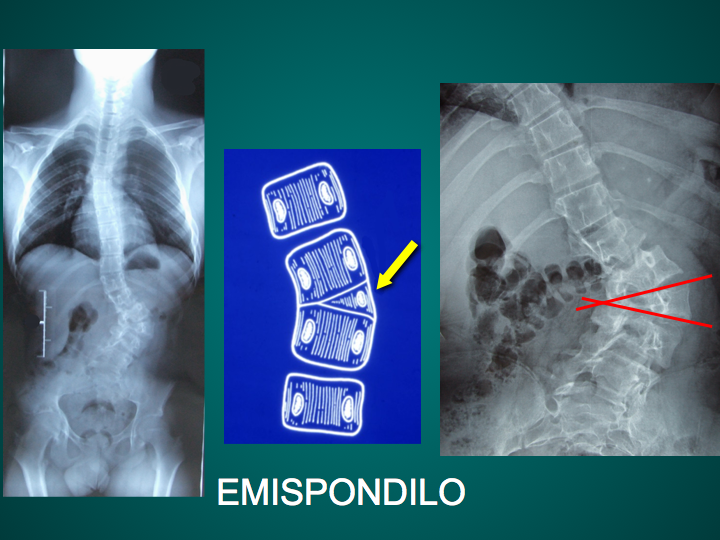
\includegraphics[width=2.39583in,height=2.28125in]{media/image9.png}
\end{quote}

\begin{itemize}
\item
  \textbf{CHIUSE}: attorno alla rima di frattura e ai monconi \emph{la
  cute è integra}
\item
  \textbf{ESPOSTE (O APERTE)} = \emph{l'integrità cutanea è interrotta}
  e il focolaio di frattura comunica con l'ambiente esterno tramite una
  ferita più o meno ampia. \emph{In questo caso il focolaio della
  frattura è esposto a contaminazione microbica che può evolvere verso
  una vera e propria osteomielite.} Sono molto importanti perché
  rappresentano delle urgenze chirurgiche.
\end{itemize}

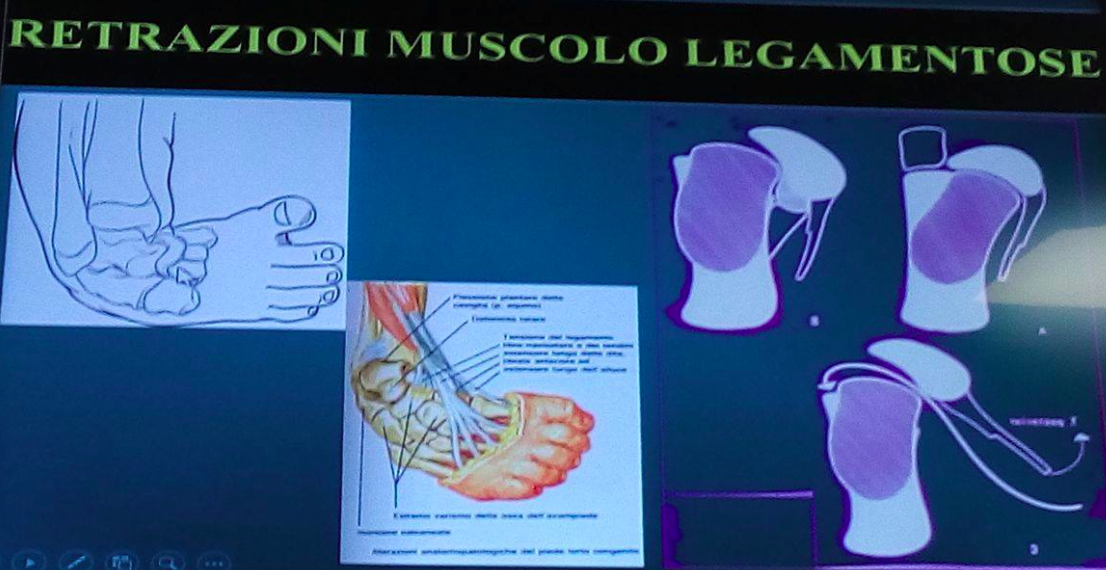
\includegraphics[width=5.41667in,height=3.25000in]{media/image10.png}

\emph{Urgenze}

\begin{itemize}
\item
  \textbf{Fratture esposte}: devono essere portate in sala operatoria
  massimo entro 6/8 ore (tempo minimo oltre il quale può insorgere
  infezione. L'infezione all'osso è difficilissima da trattare perché
  l'osso è già di per sé un tessuto a cui arriva poco sangue e in uno
  danneggiato ne arriva ancora meno). Nel minor tempo possibile
  l'ortopedico deve pulire il focolaio, rimuovere i tessuti necrotici,
  stabilizzare con un fissatore a ponte e coprire il più possibile con
  muscoli, sottocute e cute la ferita.
\item
  \textbf{Distacchi epifisari}: parliamo di distacco epifisario quando,
  nei bambini e nei giovani adulti, si osserva la separazione traumatica
  dell'epifisi dalla metafasi alla quale aderisce per interposizione
  della cartilagine di accrescimento (la rima di frattura passa
  attraverso la cartilagine di accrescimento). Ricordate che il tessuto
  cartilagineo fertile guida l'accrescimento delle ossa lunghe. Possono
  essere distinti in:
\end{itemize}

\begin{itemize}
\item
  \textbf{Puri}: è interessata \emph{solo} la cartilagine di
  accrescimento.
\item
  \textbf{Misti:} la rima di frattura di estende al tessuto contiguo
  perciò sono interessate la cartilagine di accrescimento e la
  cartilagine sopra e/o sottostante.
\end{itemize}

\begin{quote}
Anche queste devono essere stabilizzate entro 6/8 ore,
l\textbf{'}obiettivo è quello di agire il prima possibile per evitare la
morte delle cellule della zona di accrescimento. Non è prevedibile se
l'accrescimento avverrà poi in maniera normale oppure no, con i genitori
bisogna essere sempre molto schietti e diretti: si vedrà nel tempo cosa
accadrà.

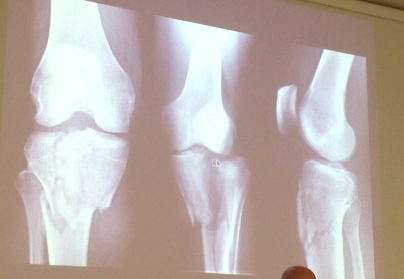
\includegraphics[width=3.73958in,height=2.86458in]{media/image11.png}
\end{quote}

\emph{La classificazione di Salter- Harris prevede la distinzione dei
distacchi epifisari in 5 tipi, in rapporto al decorso della rima di
frattura}

\begin{quote}
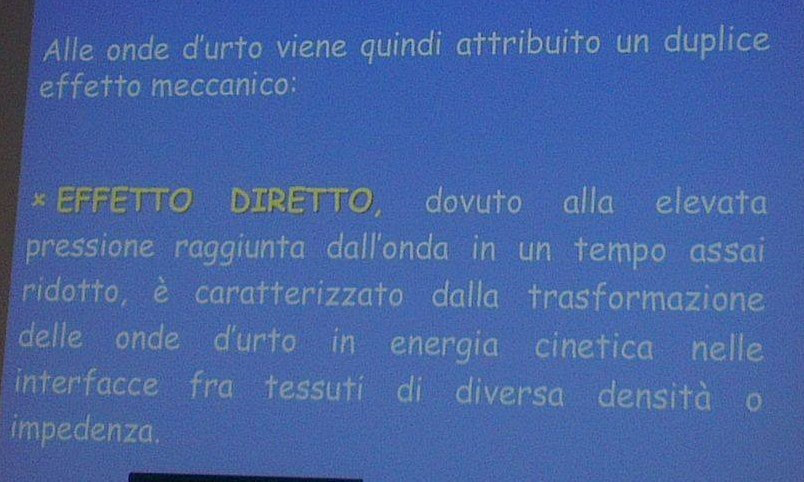
\includegraphics[width=4.06458in,height=3.46875in]{media/image12.jpeg}

Possibili inconvenienze in caso di distacchi epifisari possono essere:
\end{quote}

\begin{itemize}
\item
  Ipometria (un arto cresce meno dell'altro)
\item
  Distorcimento (un arto cresce storto)
\end{itemize}

\begin{itemize}
\item
  \textbf{FRATTURA-LUSSAZIONE}: Definiamo la lussazione come una perdita
  \emph{permanente} dei rapporti tra due capi articolari (il classico
  esempio è quando un soggetto cade e si ha lussazione della spalla: si
  dice che la spalla ``esce'' e non si riesce a ``rimetterla dentro'').
  La lussazione è da differenziare invece dalla distorsione definita
  come una perdita \emph{temporanea} dei rapporti tra due capi
  articolari.
\end{itemize}

Le lussazioni sono delle emergenze e devono essere trattate applicando
una trazione per rimettere a posto i capi articolari. Quando siamo di
fronte ad una lussazione prima di fare qualsiasi manovra dobbiamo sempre
eseguire un RX per valutare la possibilità che ci sia anche una
frattura. L'RX va sempre eseguita anche dopo la manovra di trazione.

\emph{Diagnosi}

Di fronte ad un sospetto clinico di frattura bisogna fare una diagnosi:
in prima battuta una diagnosi clinica che dovrà poi essere confermata
con delle indagini strumentali.

\textbf{Diagnosi clinica}:

Di fronte ad un sospetto di frattura avremo:

\begin{itemize}
\item
  \textbf{Segni di probabilità}
\end{itemize}

\begin{itemize}
\item
  \emph{Atteggiamento} ad esempio l'extra-rotazione e accorciamento
  della gamba indicano una possibile frattura del femore
\item
  \emph{Deformità} ad esempio il dorso a forchetta nella frattura di
  polso
\end{itemize}

\begin{quote}
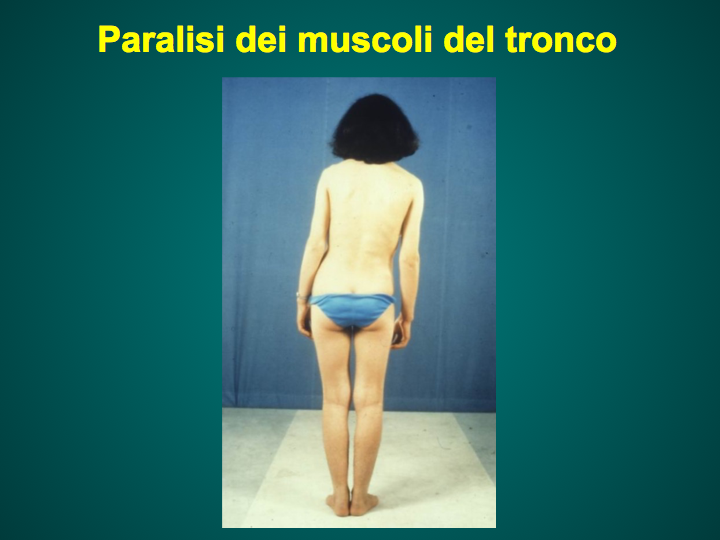
\includegraphics[width=4.77083in,height=2.91667in]{media/image13.png}
\end{quote}

\begin{itemize}
\item
  \emph{Ferite/ ecchimosi}
\item
  \emph{Tumefazioni e lesioni cutanee}
\item
  \emph{Dolore importante}
\item
  \emph{Impotenza funzionale} ad esempio il paziente non riesce a
  muovere l'arto interessato o a camminare
\end{itemize}

\begin{itemize}
\item
  \textbf{Segni di certezza }
\end{itemize}

\begin{itemize}
\item
  \emph{Crepitio}: dovuto ai due monconi di frattura che stridono l'uno
  sull'altro.
\item
  \emph{Motilità preternaturale} ad esempio prendo in mano un arto e
  vedo che si piega in maniera innaturale).
\end{itemize}

\begin{quote}
La diagnosi clinica deve poi essere sempre confermata dalle indagini
strumentali che permettono di poter pianificare un corretto trattamento
e che sono molto importanti dal punto di vista medico-legale. Le
principali sono:
\end{quote}

\begin{itemize}
\item
  \emph{RX STANDARD}: da eseguire in tutte le posizioni
  (antero-laterale, latero-laterale e obliqua) per avere una visione
  completa della frattura. È un esame che si deve eseguire SEMPRE nel
  sospetto di una frattura e molto spesso è dirimente.
\item
  \emph{TAC}: si esegue quando l'RX è negativa, ma il sospetto clinico
  di frattura è ancora fortemente presente (ad esempio quando c'è un
  dolore importante). A volte può far vedere delle fratture che con una
  normale RX non si vedono.
\end{itemize}

\begin{quote}
Viene anche richiesta per uno studio morfologico della frattura e per un
pianificazione pre-operatoria.

Non si esegue nei bambini perché utilizza radiazioni ionizzanti.
\end{quote}

\begin{itemize}
\item
  \emph{RMN}: utilizzata nei bambini al posto della TAC anche se risulta
  essere meno sensibile e meno specifica di quest'ultima. Rappresenta un
  ottimo mezzo per scoprire le fratture da stress.
\item
  \emph{SCINTIGRAFIA:} caduta completamente in disuso con l'introduzione
  della RMN.
\end{itemize}

\end{document}

\documentclass[]{article}
\usepackage{lmodern}
\usepackage{amssymb,amsmath}
\usepackage{ifxetex,ifluatex}
\usepackage{fixltx2e} % provides \textsubscript
\ifnum 0\ifxetex 1\fi\ifluatex 1\fi=0 % if pdftex
  \usepackage[T1]{fontenc}
  \usepackage[utf8]{inputenc}
\else % if luatex or xelatex
  \ifxetex
    \usepackage{mathspec}
  \else
    \usepackage{fontspec}
  \fi
  \defaultfontfeatures{Ligatures=TeX,Scale=MatchLowercase}
\fi
% use upquote if available, for straight quotes in verbatim environments
\IfFileExists{upquote.sty}{\usepackage{upquote}}{}
% use microtype if available
\IfFileExists{microtype.sty}{%
\usepackage{microtype}
\UseMicrotypeSet[protrusion]{basicmath} % disable protrusion for tt fonts
}{}
\usepackage[unicode=true]{hyperref}
\hypersetup{
            pdfborder={0 0 0},
            breaklinks=true}
\urlstyle{same}  % don't use monospace font for urls
\usepackage{graphicx,grffile}
\makeatletter
\def\maxwidth{\ifdim\Gin@nat@width>\linewidth\linewidth\else\Gin@nat@width\fi}
\def\maxheight{\ifdim\Gin@nat@height>\textheight\textheight\else\Gin@nat@height\fi}
\makeatother
% Scale images if necessary, so that they will not overflow the page
% margins by default, and it is still possible to overwrite the defaults
% using explicit options in \includegraphics[width, height, ...]{}
\setkeys{Gin}{width=\maxwidth,height=\maxheight,keepaspectratio}
\IfFileExists{parskip.sty}{%
\usepackage{parskip}
}{% else
\setlength{\parindent}{0pt}
\setlength{\parskip}{6pt plus 2pt minus 1pt}
}
\setlength{\emergencystretch}{3em}  % prevent overfull lines
\providecommand{\tightlist}{%
  \setlength{\itemsep}{0pt}\setlength{\parskip}{0pt}}
\setcounter{secnumdepth}{0}
% Redefines (sub)paragraphs to behave more like sections
\ifx\paragraph\undefined\else
\let\oldparagraph\paragraph
\renewcommand{\paragraph}[1]{\oldparagraph{#1}\mbox{}}
\fi
\ifx\subparagraph\undefined\else
\let\oldsubparagraph\subparagraph
\renewcommand{\subparagraph}[1]{\oldsubparagraph{#1}\mbox{}}
\fi

% set default figure placement to htbp
\makeatletter
\def\fps@figure{htbp}
\makeatother


\date{}

\begin{document}

\emph{Le fratture vertebrali}

Si tratta di fratture abbastanza frequenti: rappresentano circa il 4\%
di tutte le fratture dello scheletro. Possono essere suddivise in:

\begin{itemize}
\item
  F\emph{ratture vertebrali traumatiche} che sono prevalenti tra la
  \emph{3° e 4° decade di vita} e interessano principalmente \emph{il
  sesso maschile}
\item
  \emph{\emph{Fratture vertebrali patologiche che colpiscono più spesso
  l'anziano e sono generalmente su base osteoporotica. Q}}ueste
  interessano soprattutto \emph{le donne in età avanzata}. \emph{Nelle
  fratture vertebrali patologiche rientrano anche quelle metastatiche}
\end{itemize}

\begin{quote}
\emph{Fratture vertebrali traumatiche}
\end{quote}

Le fratture vertebrali \emph{traumatiche} interessano (in ordine
decrescente):

\begin{itemize}
\item
  Il tratto dorso-lombare più frequentemente ed esattamente il punto di
  maggiore mobilità: il punto di passaggio tra la colonna toracica e la
  colonna lombare (T11-T12-L1)
\item
  Il tratto cervicale
\item
  Il tratto lombare
\item
  Il tratto toracico.
\end{itemize}

Le fratture vertebrali \emph{traumatiche} possono essere suddivise in:

\begin{itemize}
\item
  \textbf{FRATTURE VERTEBRALI AMIELICHE} → Senza interessamento
  neurologico
\item
  \textbf{FRATTURE VERTEBRALI MIELICHE} → Con interessamento
  neurologico. Sono caratterizzate da \emph{lesioni del midollo spinale}
  oppure \emph{delle radici nervose} che emergono dai forami di
  coniugazione tra una vertebra e l'altra. La gravità e l'estensione del
  danno neurologico dipendono dalla sede della lesione: il danno sarà
  tanto più severo quanto più è alta la lesione midollare quindi una
  lesione del rachide cervicale sarà più grave rispetto ad una lesione
  del tratto lombare. Fratture \emph{cervicali alte} (frattura di C1)
  tipo fratture \emph{del dente dell'epistrofeo} (fratture di C2 o C3)
  possono condurre alla \emph{morte del paziente per coinvolgimento dei
  centri nervosi del respiro}. Ci sono pazienti con fratture cervicali
  alte che oltre ad essere tetraplegici hanno anche difficoltà a
  respirare, a deglutire a parlare.
\end{itemize}

\begin{quote}
Nelle fratture mieliche la lesione del tessuto nervoso può essere
conseguente a:
\end{quote}

\begin{enumerate}
\def\labelenumi{\arabic{enumi}.}
\item
  \textbf{Compressione diretta} →in seguito alla frattura, un frammento
  osseo \emph{(di un corpo vertebrale, di un arco, di un peduncolo di
  una vertebra)} va a schiacciare/toccare il midollo \emph{o una delle
  radici nervose e dà una sintomatologia periferica per:}
\end{enumerate}

\begin{itemize}
\item
  \emph{Per compressione}
\item
  \emph{Per lesione (il midollo viene sezionato in parte o
  completamente)}
\end{itemize}

\begin{enumerate}
\def\labelenumi{\arabic{enumi}.}
\item
  \textbf{Scivolamento di una vertebra sulla sottostante} (raro) → si ha
  una lesione da taglio. \emph{Quando ad una frattura di un corpo
  vertebrale si associa una lussazione (cioè una dislocazione del corpo
  vertebrale rispetto al sottostante) ciò che sta nel mezzo viene
  lesionato o sezionato.} Sì immagini di avere un tubo in gomma con
  dentro dell'acqua: spostando la parte sottostante rispetto a quella
  sovrastante l'acqua uscirà sia da sopra che da sotto il tubo (lo
  stesso meccanismo si può avere a livello del midollo)
\item
  \textbf{Ematomielia post-traumatica} → in seguito alla frattura si
  verifica un sanguinamento importante (l'osso quando si frattura
  sanguina molto) e si forma un ematoma che va a comprimere il midollo
\end{enumerate}

\begin{quote}
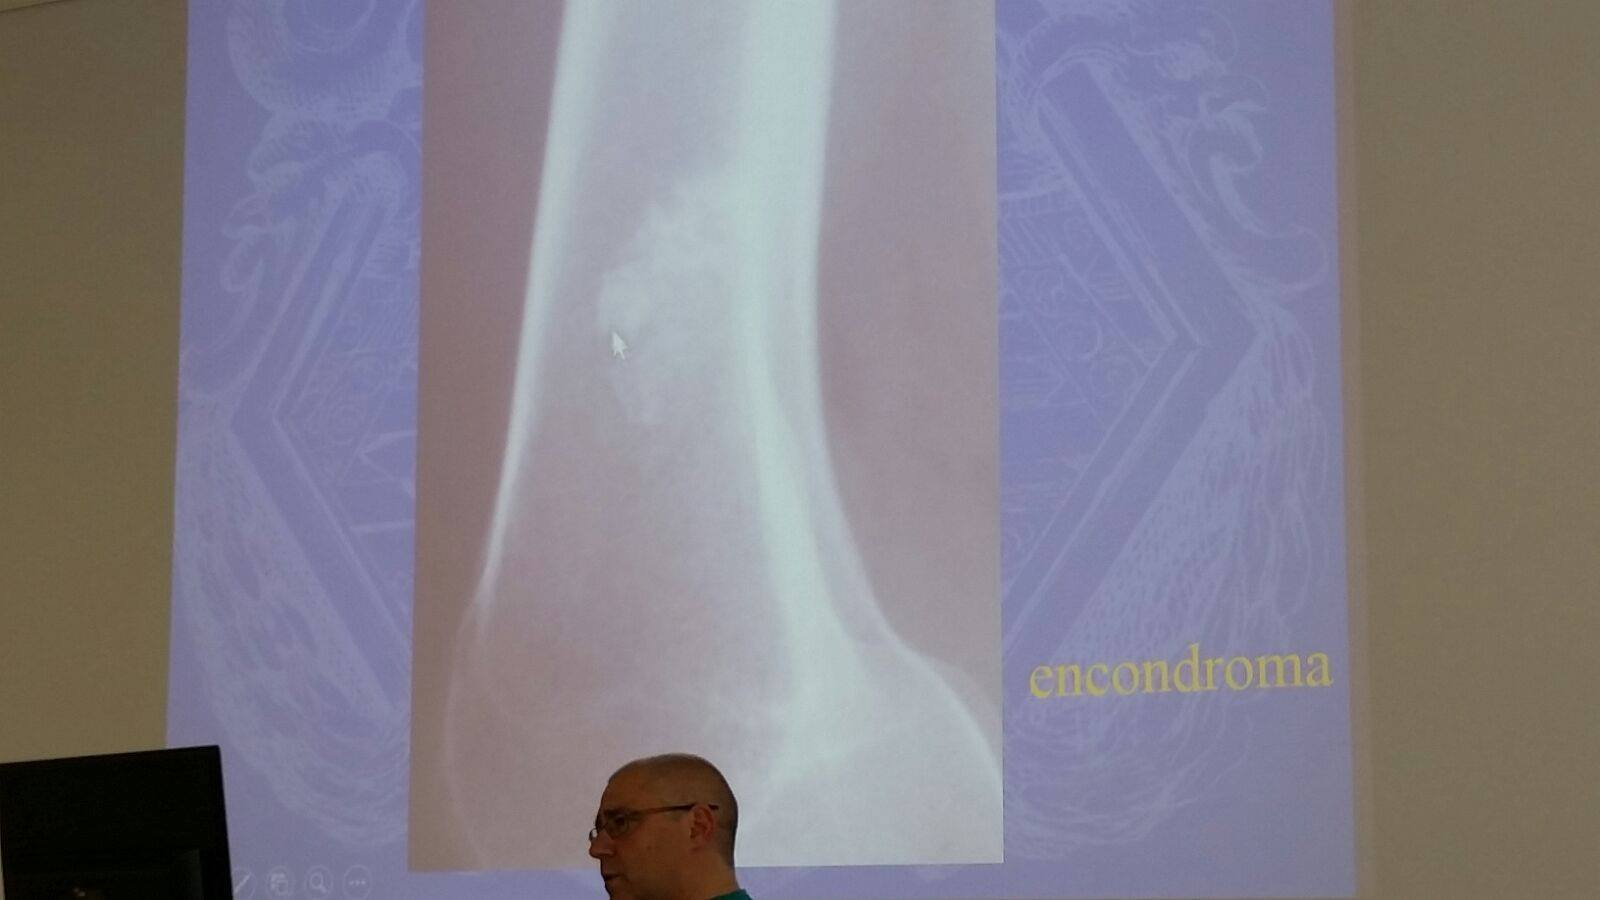
\includegraphics[width=4.66667in,height=3.42708in]{media/image1.jpeg}
\end{quote}

\emph{Classificazione}

Classificazione basata sul \emph{punto della vertebra} in cui queste
lesioni avvengono:

\begin{itemize}
\item
  Fratture \emph{anteriori isolate} o del \emph{corpo vertebrale} (le
  più frequenti)
\item
  Fratture della \emph{parte posteriore} o \emph{arcali}
\item
  Fratture \emph{totali} (corpo e archi)
\item
  Fratture isolate \emph{dei peduncoli}, \emph{\emph{degli archi}}, dei
  \emph{processi trasversi} o \emph{spinosi (raramente)}
\item
  \emph{Fratture-lussazioni} (casi più gravi, \emph{ma fortunatamente
  molto rari}): sono fratture associate ad una lussazione e quindi ad
  una instabilità articolare (es. spostamento di una vertebra rispetto a
  quella sottostante)
\item
  \emph{Fratture multiple} che interessano per esempio corpo, peduncolo,
  processo spinoso, processo trasverso.
\end{itemize}

\emph{Clinica}

Consideriamo i due casi

\textbf{FRATTURE VERTEBRALI AMIELICHE }

\begin{itemize}
\item
  Dolore locale in corrispondenza della zona interessata dalla frattura
\item
  Impotenza e limitazione funzionale: \emph{il paziente non riesce a
  piegarsi completamente sul tronco o a compiere i movimenti che
  normalmente e quotidianamente fa}
\item
  Alterazioni dell'atteggiamento della colonna: cifosi reattiva e/o
  scoliosi reattiva in vicinanza della frattura
\item
  Contrattura muscolare antalgica reattiva dei muscoli paravertebrali:
  \emph{per riflesso al dolore questi muscoli contraggono e determinano
  una \emph{scoliosi antalgica} del rachide, accompagnata dalla
  contrattura stessa, che è palpabile.}
\end{itemize}

\textbf{MIELICHE CLINICA }

\begin{itemize}
\item
  Dolore locale
\item
  Impotenza e limitazione funzionale
\item
  Alterazioni dell'atteggiamento della colonna (cifosi e/o scoliosi)
\item
  Contrattura muscolare antalgica
\item
  Sintomatologia neurologica in rapporto alla sede e all'entità del
  trauma (37\% rachide cervicale, 22\% rachide dorsale ,8\% rachide
  lombare). Un paziente con una frattura mielica in T7, T8, T9, T12 avrà
  paraplegia (paralisi di entrambi gli arti inferiori) associata ad
  alterazioni sfinteriche sia delle vie urinarie che dell'apparato
  gastrointestinale. Un paziente che avrà una frattura mielica di C6, C7
  avrà una tetraplegia (paralisi di tutti gli arti). La clinica varia a
  seconda del livello della lesione midollare.
\end{itemize}

\emph{Diagnosi}

AMIELICHE/MIELICHE DIAGNOSI

\begin{itemize}
\item
  Anamnesi
\item
  Esame obiettivo
\item
  Esami strumentali → Radiografia, TAC, RMN, Scintigrafia
\end{itemize}

Iter in caso di trauma del rachide → il primo passaggio è
l'immobilizzazione, possibilmente in barella cucchiaio. Se si sospetta
un interessamento del rachide cervicale, si deve fare indossare al
paziente un collare. In PS viene fatta di base una radiografia del
rachide interessato. La radiografia deve essere fatta in tutte e tre le
proiezioni: anteroposteriore, latero-laterale, obliqua.

Iter nei politraumi → fare una TAC di tutto il rachide (senza passare
attraverso la radiografia). Qualora ci sia una frattura mielica, in PS,
è indicato eseguire anche una RMN che, oltre ad indicarci il danno
osseo, ci permetterà di individuare la presenza e l'entità di ematomi e
danni midollari dal momento che \emph{studia meglio i tessuti molli.}

Altro punto è la valutazione dell'entità del trauma in una frattura
mielinica, tale trauma potrà determinare delle condizioni più o meno
reversibili:

\begin{itemize}
\item
  Commozione midollare che è sempre reversibile→ prognosi migliore. Si
  potrebbe fare un paragonare con il colpo del K.O nel pugilato (il
  sistema nervoso va in tilt per un attimo e poi si riprende).
\item
  Contusione midollare che invece non è sempre e del tutto reversibile
  →quadro più grave rispetto al precedente. Il tessuto nervoso in
  corrispondenza della frattura ha subito una contusione cioè una sorta
  di trauma diretto. La RMN in questo caso può mostrare un edema del
  tessuto nervoso perifratturativo.
\item
  Compressione midollare che è parzialmente reversibile se dura però
  poche ore → Il tessuto nervoso ha avuto un trauma diretto che persiste
  attraverso un meccanismo compressivo (per esempio un frammento d'osso
  che schiaccia il midollo oppure la presenza di un ematoma che comprime
  il midollo). Non c'è sezione del midollo.
\item
  Sezione midollare che è sempre irreversibile → quadro grave in cui il
  midollo è stato sezionato, tagliato, distrutto. Lo stesso discorso
  vale per le radici nervose: quando vengono sezionate (``strappate'')
  non si riparano quasi mai. \emph{Discorso diverso vale per il tessuto
  nervoso periferico}: una lesione da taglio del nervo mediano o del
  nervo radiale o del nervo ulnare guarisce, soprattutto se suturata
  microchirurgicamente con precisione e non in tensione. I nervi
  periferici iniziano a rigenerare 15-20 giorni dopo la sutura:1 mm al
  giorno (ricrescono in un certo senso). Di fronte ad una grossa lesione
  del SNP bisogna essere sempre cauti nel garantire una restitutio ad
  integrum della funzione del nervo.
\end{itemize}

\emph{Terapia}

Il trattamento per le fratture vertebrali può essere di 2 tipi;

\begin{itemize}
\item
  \textbf{Conservativo}: impiego di busti in gesso o di tutori
  ortopedici che di solito nel paziente giovane devono essere tenuti per
  almeno tre mesi e poi abbandonati gradualmente. Questo tipo di
  trattamento è indicato nelle \emph{fratture stabili e amieliche}.
  Concetto di \textbf{stabilità}: \emph{una frattura è stabile se dal
  punto di vista morfologico e strutturale si è sicuri che quella
  frattura non si scomporrà andando a comprimente il midollo. La
  frattura rimarrà in quella posizione}. Una frattura amielica stabile
  rimarrà amielica poiché i frammenti ossei non si sposteranno e
  \emph{non andranno a determinare un danno nervoso}. Proprio per tale
  caratteristica il trattamento sarà fondamentalmente di
  immobilizzazione mediante busti in gesso o ortopedici. \emph{In queste
  fratture la sintomatologia clinica regredisce più rapidamente rispetto
  alla velocità con cui si vede la guarigione alle radiografie (non c'è
  corrispondenza tra clinica e processo di guarigione).}
\end{itemize}

\emph{Il busto va tenuto almeno 3 mesi. Di solito l'iter è:}

\begin{itemize}
\item
  \emph{Busto per 35-40 giorni}
\item
  \emph{Si toglie il busto e si fa un RX di controllo}
\item
  \emph{Si applica un altro busto di solito ortopedico per altri 40-45
  giorni,}
\item
  \emph{Segue, se la radiografia va bene, un progressivo svezzamento dal
  busto con fisioterapia per recuperare l'articolarità del rachide.}
\end{itemize}

\emph{Nei primi giorni post-trauma per riflesso il paziente può avere un
alterazione dell'alvo e/o della diuresi: infatti prima di fare il busto
dobbiamo aspettare che il paziente si canalizzi mentre per la diuresi si
può mettere il catetere; si consiglia in seguito al paziente una dieta
ricca di fibre.}

\begin{itemize}
\item
  \textbf{Chirurgico:}
\end{itemize}

\begin{itemize}
\item
  Nel caso in cui la frattura sia \emph{amielica instabile} cioè con
  caratteristiche morfologiche che fanno pensare ad una possibile
  scomposizione della frattura e ad un possibile danno del tessuto
  nervoso. Si dovrà intervenire chirurgicamente andando a stabilizzare
  la colonna vertebrale nei giorni successivi al trauma \emph{(non in
  urgenza)}.
\item
  Nel caso in cui la frattura sia \emph{mielica e instabile}. In questo
  caso si dovrà intervenire chirurgicamente \emph{in urgenza} poiché,
  come visto in precedenza, ci potranno essere delle condizioni di danno
  nervoso potenzialmente reversibili. In questo ultimo caso, come per le
  fratture esposte, si pone un limite temporale tra le 6 e 8 ore dal
  trauma.
\end{itemize}

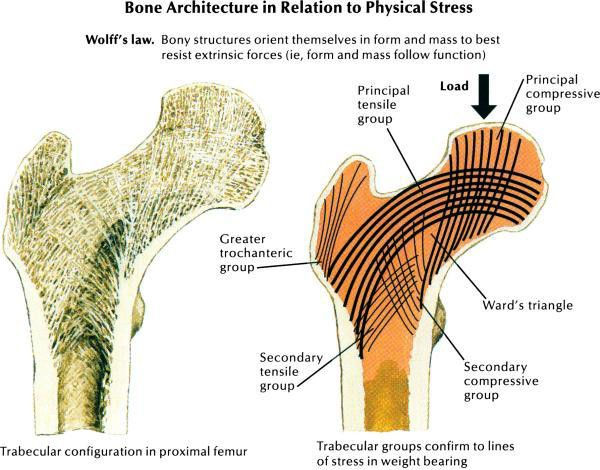
\includegraphics[width=4.69792in,height=3.52083in]{media/image2.jpeg}

In questa radiografia (in alto a sx) della colonna vertebrale si possono
osservare corpi vertebrali normali con la tipica conformazione
rettangolare e un corpo vertebrale diverso dagli altri. Quest'ultimo è
schiacciato: è deformato a cuneo. È una frattura amielica e per valutare
la stabilità è stata fatta una TAC (in alto a dx) in cui si vede il
corpo vertebrale fratturato che è più basso rispetto agli altri e si può
notare la presenza di un frammento osseo che protrude nel canale
vertebrale con conseguente restringimento dello stesso. Ne deduciamo che
questa frattura potenzialmente potrebbe diventare mielica e perciò
instabile. In questo caso è stato fatto un intervento chirurgico di
riduzione e stabilizzazione con delle barre e viti peduncolari (cioè che
passano attraverso i peduncoli vertebrali e vanno a fissarsi all'interno
del corpo vertebrale) che vanno messe sopra e sotto il corpo vertebrale
fratturato. È stato cosi stabilizzato il corpo vertebrale lesionato.
Questo tipo di stabilizzazione nelle fratture amieliche è sufficiente
mentre nelle fratture mieliche può essere indicato fare una
decompressione del canale midollare: evacuazione dell'ematoma o
decompressione mediante spostamento dei frammenti ossei.

\emph{Fratture vertebrali patologiche su base osteoporotica}

Sono molto diffuse tra la popolazione anziana. A \emph{differenza} delle
fratture traumatiche:

\begin{itemize}
\item
  Sono \emph{fratture vertebrali patologiche}
\item
  Colpiscono generalmente l'individuo \emph{anziano}
\item
  Sono legate \emph{a traumi di minima entità} piuttosto che ad un
  trauma efficiente. \emph{Molto spesso il paziente non riferisce traumi
  oppure ne riporta di modesti:} una banale caduta in casa, alzarsi
  improvvisamente dal letto
\item
  \emph{Il sesso femminile è prevalentemente interessato}.
\end{itemize}

\begin{quote}
Possiamo definirle come una sorta di \emph{cedimento strutturale} dei
corpi vertebrali. Raramente sono localizzate ad un unico segmento
piuttosto \emph{interessano segmenti multipli}. La \emph{deformità}
evidente all'esame radiologico è definita \emph{``a cuneo'' o ``a lente
biconcava''} (vedi immagina sotto)
\end{quote}

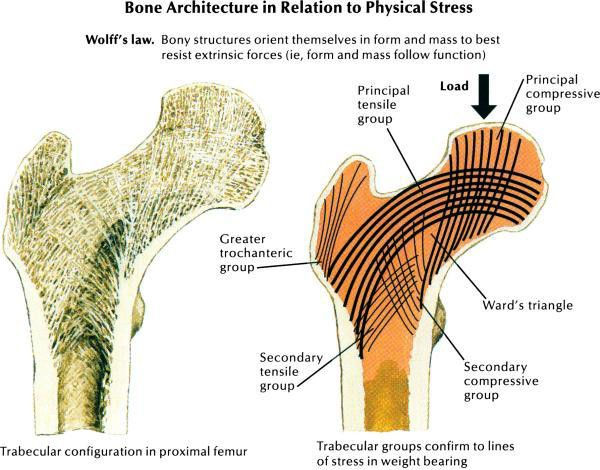
\includegraphics[width=4.16667in,height=3.13542in]{media/image3.jpeg}

Questo è un esempio di frattura vertebrale ben evidenziata
radiograficamente. Da notare è la deformità a cuneo del corpo vertebrale

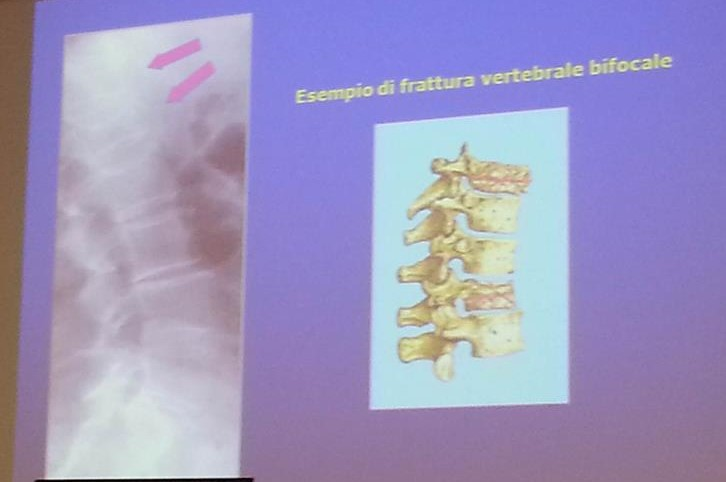
\includegraphics[width=4.19792in,height=2.79167in]{media/image4.jpeg}

Esempio di frattura vertebrale bifocale → il piatto del corpo vertebrale
superiormente si schiaccia e lo stesso accade per il piatto del corpo
vertebrale inferiore.

\emph{Clinica}

La sintomatologia nelle fratture vertebrali da osteoporosi non è
particolarmente importante. Il dolore non è acuto, ma di tipo
progressivo: legato al movimento, più sordo rispetto al dolore di quelle
traumatiche.

\emph{Terapia}

Nella maggior parte dei casi si sceglie \emph{un trattamento incruento}
e di \emph{tipo conservativo} basato sulla applicazione di busti
ortopedici:

\begin{itemize}
\item
  Nel \emph{giovane} si preferiscono \emph{busti fissi metallici} per la
  \emph{stabilizzazione} di queste fratture
\item
  Nell'anziano affetto da comorbilità (problemi respiratori, problemi
  cardiovascolari, problemi addominali) si preferiscono \emph{busti in
  stoffa armata} (panciere di stoffa dotate di legacci e posteriormente
  di barre metalliche che sostengono la colonna vertebrale) fatti su
  misura. \emph{La scelta è dettata dal fatto che il paziente anziano
  non sopporta facilmente busti metallici o in gesso.} Questo tipo di
  trattamento ortopedico è finalizzato alla guarigione della frattura;
  dopodiché si cercherà di prevenire nuove fratture e il peggioramento
  dell'avvallamento dei corpi vertebrali attraverso una \emph{terapia
  sostitutiva per l'osteoporosi a base di calcio vit.D e bifosfonati.}
\end{itemize}

In \emph{alcuni casi} si potrà intervenire attraverso una \emph{metodica
più invasiva} che di solito viene eseguita dal radiologo interventista:

\begin{itemize}
\item
  \textbf{Vertebroplastica} → introduzione attraverso \emph{una
  cannula}, per via percutanea (attraverso i peduncoli vertebrali nel
  corpo vertebrale fratturato), di metilmetacrilato (cemento acrilico)
  con lo scopo di aumentar la rigidità e la resistenza meccanica della
  vertebra al carico in compressione e \emph{nello stesso tempo
  alleviare il dolore}. È eseguita sotto controllo della radioscopia.
  Nel caso di una paziente con una vertebra osteoporotica schiacciata,
  datata da alcune settimane, che tende progressivamente a peggiorare e
  che provoca molto dolore, posso eseguire una vertebroplastica. Il
  cemento acrilico una volta iniettato si solidificherà e bloccherà il
  progressivo schiacciamento del corpo vertebrale. Come se cementassimo
  la colonna vertebrale.
\end{itemize}

\begin{itemize}
\item
  \textbf{Cifoplastica}→ introduzione per via percutanea, attraverso i
  peduncoli, nel corpo vertebrale fratturato, di metimetacrilato. Come
  nel caso precedente però la manovra è preceduta dall' introduzione
  nello stesso corpo vertebrale di un palloncino espansibile che ha lo
  scopo di ridurre la deformità della vertebra fratturata e di creare lo
  spazio vuoto in cui il cemento possa penetrarvi con facilità.
  Attraverso il palloncino si cerca di recuperare l'altezza del corpo
  vertebrale fratturato mentre attraverso il cemento acrilico si cerca
  di mantenere questa altezza recuperata ed evitare uno schiacciamento.
\end{itemize}

\emph{La scelta tra queste due procedure sarà influenzata da:}

\begin{itemize}
\item
  \emph{Qualità ossea }
\item
  \emph{Tempistica di arrivo del paziente }
\item
  \emph{Diagnosi della frattura.}
\end{itemize}

\begin{quote}
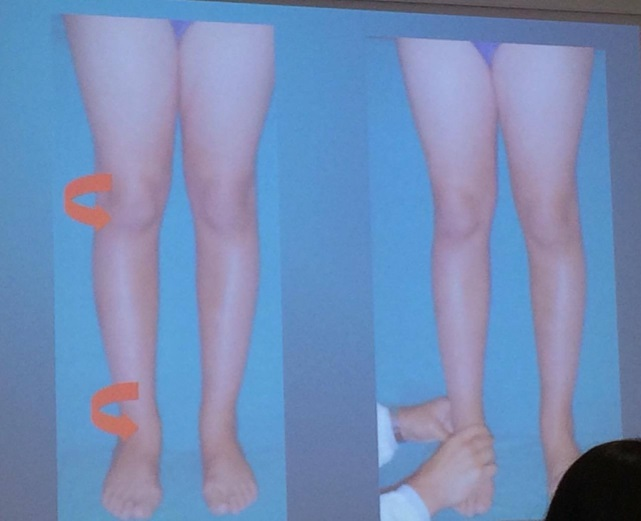
\includegraphics[width=4.18750in,height=3.00000in]{media/image5.jpeg}

Le due procedure di cui sopra si eseguono in sala operatoria, in
anestesia peridurale o generale sotto controllo radioscopico. Quando
siamo sicuri di essere all'interno del corpo vertebrale con una sorta di
cannula viene iniettato questo cemento che da prima è semiliquido e nel
corso di pochi minuti diventa solido.

\includegraphics[width=2.55208in,height=2.75000in]{media/image6.jpeg}

Immagine in laterale del cemento immesso nel contesto del corpo
vertebrale. Si vede una vertebra con il cemento e un'altra senza
cemento.
\end{quote}

\textbf{Complicanze vertebroplastica} → il cemento iniettato all'interno
del corpo vertebrale potrebbe fuoriuscire nel canale vertebrale con
conseguenti:

\begin{itemize}
\item
  Danni nervosi
\item
  Danneggiamento delle strutture attorno al canale vertebrale come vasi
  e nervi.
\end{itemize}

Inoltre questo intervento viene eseguito in anestesia quindi ci sono
tutte le complicanze legate alla sedazione. Ci sono controindicazioni
per:

\begin{itemize}
\item
  Pazienti scoagulati
\item
  Pazienti con problemi cardiaci
\item
  Pazienti debilitati in generale
\end{itemize}

A volte la vertebroplastica viene eseguita \emph{in pazienti neoplastici
che hanno metastasi ossee per alleviare il dolore.}

Iter riabilitativo nel paziente che ha avuto fratture ossee a causa
dell'osteoporosi:

\begin{itemize}
\item
  Curare le fratture
\item
  Prevenire altre fratture attraverso la cura dell'osteoporosi
\item
  Svolgere attività fisica moderate (camminare, fare ginnastica)
\end{itemize}

\emph{Fratture scafoide carpale e di polso}

\emph{Anatomia}

\begin{quote}
Lo scafoide carpale è un osso che fa parte della prima filiera del carpo
ed è chiamato scafoide o navicolare proprio perché ha la forma di una
nave. È ampiamente rivestito di cartilagine ialina \emph{\emph{di tipo
articolare}} eccetto una piccola regione in cui si inseriscono i
legamenti trasversi del carpo e avviene la penetrazione dei vasi
ematici. \emph{Inoltre è completamente immerso all'interno del liquido
sinoviale.} Queste caratteristiche ne fanno un osso importante nella
biomeccanica del carpo.

Prima filiera del carpo→ scafoide (il più radiale), semilunare,
piramidale, pisiforme

Seconda filiera del carpo → trapezio, trapezoide, capitato, uncinato

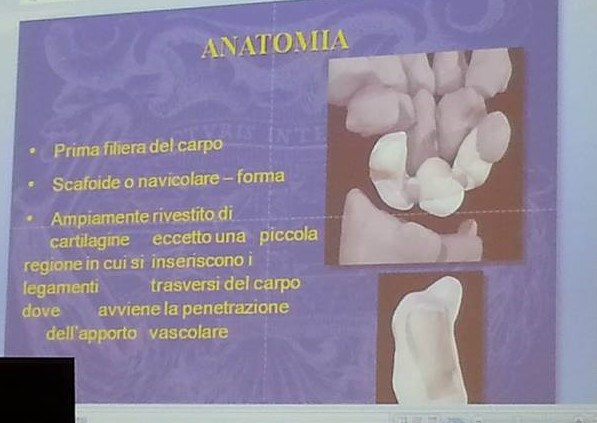
\includegraphics[width=4.91667in,height=3.48958in]{media/image7.jpeg}

All'osso scafoide arriva di base poco sangue e né arriverà ancora meno
nel momento in cui si frattura. Inoltre ha una \emph{vascolarizzazione}
di \emph{tipo terminale} (ramo dell'arteria radiale) e avviene \emph{in
maniera retrograda} ossia \emph{il sangue penetra dal polo distale dello
scafoide e va a vascolarizzare il polo prossimale}. Da quanto detto si
può facilmente capire perché le fratture del polo distale avranno una
prognosi migliore: il \emph{sangue arriva prima e in quantità maggiore}
rispetto a quelle del polo prossimale in cui il sangue arriva dopo e in
minor quantità.

Epidemiologia

\emph{Queste fratture sono più frequenti nel giovane maschio adulto:}
\end{quote}

\begin{itemize}
\item
  \emph{In una bassa percentuale dei casi (2-3\%) sono bilaterali}
\item
  \emph{La maggior parte dei pz ha meno di 30 anni}
\item
  \emph{Viene colpito maggiormente il lato dominante}
\item
  \emph{Nell'85\% dei casi sono lesioni isolate (ossia solo fratture di
  scafoide)}
\item
  \emph{Nel 15\% sono associate ad altre lesioni della mano o del polso
  come per esempio fratture del radio associate o lesioni legamentose
  dei legamenti intra carpali.}
\end{itemize}

\begin{quote}
\emph{Non di rado queste fratture vengono riconosciute a distanza di
15-20-30 giorni quando la frattura non è più tale ed è diventata una
\textbf{\emph{pseudoartrosi}}. Le caratteristiche generale dell'osso
(vascolarizzazione, immersione nel liquido sinoviale, ritardo di
calcificazione rispetto alle altre ossa) lo rendono già di base più
suscettibile alla pseudoartrosi. In caso di fratture non riconosciute e
trattare tempestivamente, si aggiunge un ulteriore fattore rappresentato
dal trauma stesso:}
\end{quote}

\begin{itemize}
\item
  \emph{Il liquido sinoviale si infiltra all'interno della frattura
  ostacolandone la guarigione}
\item
  \emph{La vascolarizzazione scarsa e di tipo terminale fa sì che, al
  momento della frattura, l'apporto di sangue sia facilmente
  insufficiente}
\item
  \emph{Lenta ossificazione}
\end{itemize}

\begin{quote}
\emph{Eziopatogenesi}

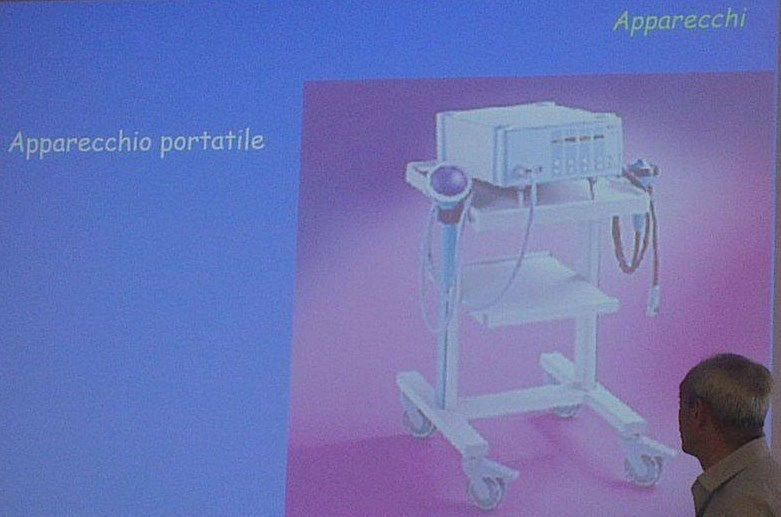
\includegraphics[width=3.77083in,height=2.82292in]{media/image8.jpeg}

Il trauma è di solito associato ad una caduta di media energia sul palmo
della mano in iperestensione dorsale: la forza lesiva viene assorbita
dall'eminenza tenar. L'estensione forzata del polso provoca
l'incuneamento dello scafoide contro il bordo dorsale del radio che
funziona da leva e può rompere lo scafoide. Ne risulta una tipica
frattura trasversa con rima decorrente nel terzo medio dello scafoide:
la frattura ha inizio sulla superficie palmare e si propaga dorsalmente

\emph{Classificazione}

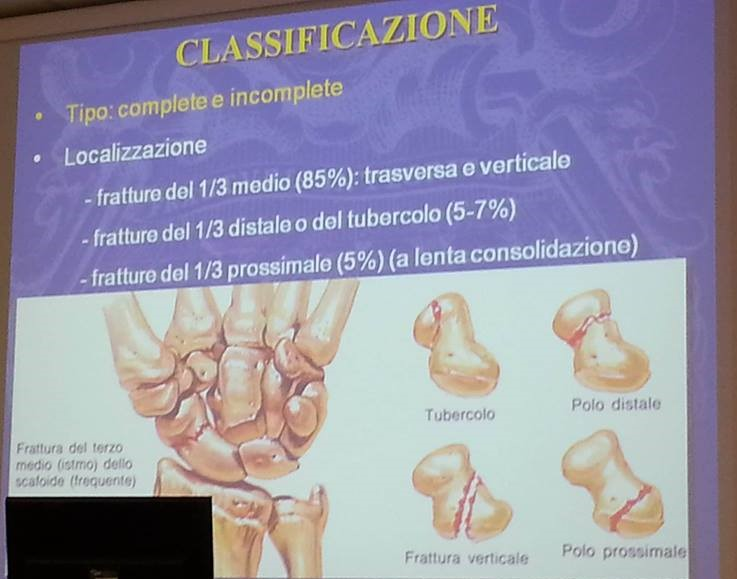
\includegraphics[width=4.15625in,height=3.26042in]{media/image9.jpeg}
\end{quote}

Vengono classificate in base:

\begin{itemize}
\item
  \emph{Tipo}:
\end{itemize}

\begin{enumerate}
\def\labelenumi{\arabic{enumi}.}
\item
  \textbf{Complete }
\item
  \textbf{Incomplete }
\end{enumerate}

\begin{itemize}
\item
  Localizzazione (è importante sapere la sede della lesione per il
  discorso fatto in precedenza sulla vascolarizzazione dello scafoide e
  perché ci dà indicazioni di tipo prognostico)
\end{itemize}

\begin{enumerate}
\def\labelenumi{\arabic{enumi}.}
\item
  Fratture del \textbf{1/3 medio} ovvero del \textbf{corpo dello
  scafoide} (85\%): trasversa (più frequente) e verticale
\item
  Fratture del \textbf{1/3 distale} o del \textbf{tubercolo} o del
  \textbf{polo distale} (5 \%) associate a una buona prognosi
\item
  Fratture del \textbf{1/3 prossimale} o \textbf{polo prossimale} (5\%).
  \emph{In questo caso entra in gioco il fattore legato alla
  vascolarizzazione di tipo retrogrado} da cui la prognosi peggiore e la
  più lenta consolidazione
\end{enumerate}

\emph{Diagnosi}

\begin{itemize}
\item
  Anamnesi positiva per trauma
\item
  Esame obiettivo:
\end{itemize}

\begin{itemize}
\item
  Dolore
\item
  Tumefazione della tabacchiera anatomica
\item
  Impotenza funzionale\emph{: il paziente fa fatica a muovere il polso
  soprattutto in alcuni tipi di movimenti cioè quelli che comportano
  prono-supinazione come avvitare o svitare un boccetto, chiudere la
  porta}
\item
  Tipico è il segno della ``o'' cioè l'esaminatore schiaccia tra pollice
  e indice lo scafoide e questo evoca dolore
\end{itemize}

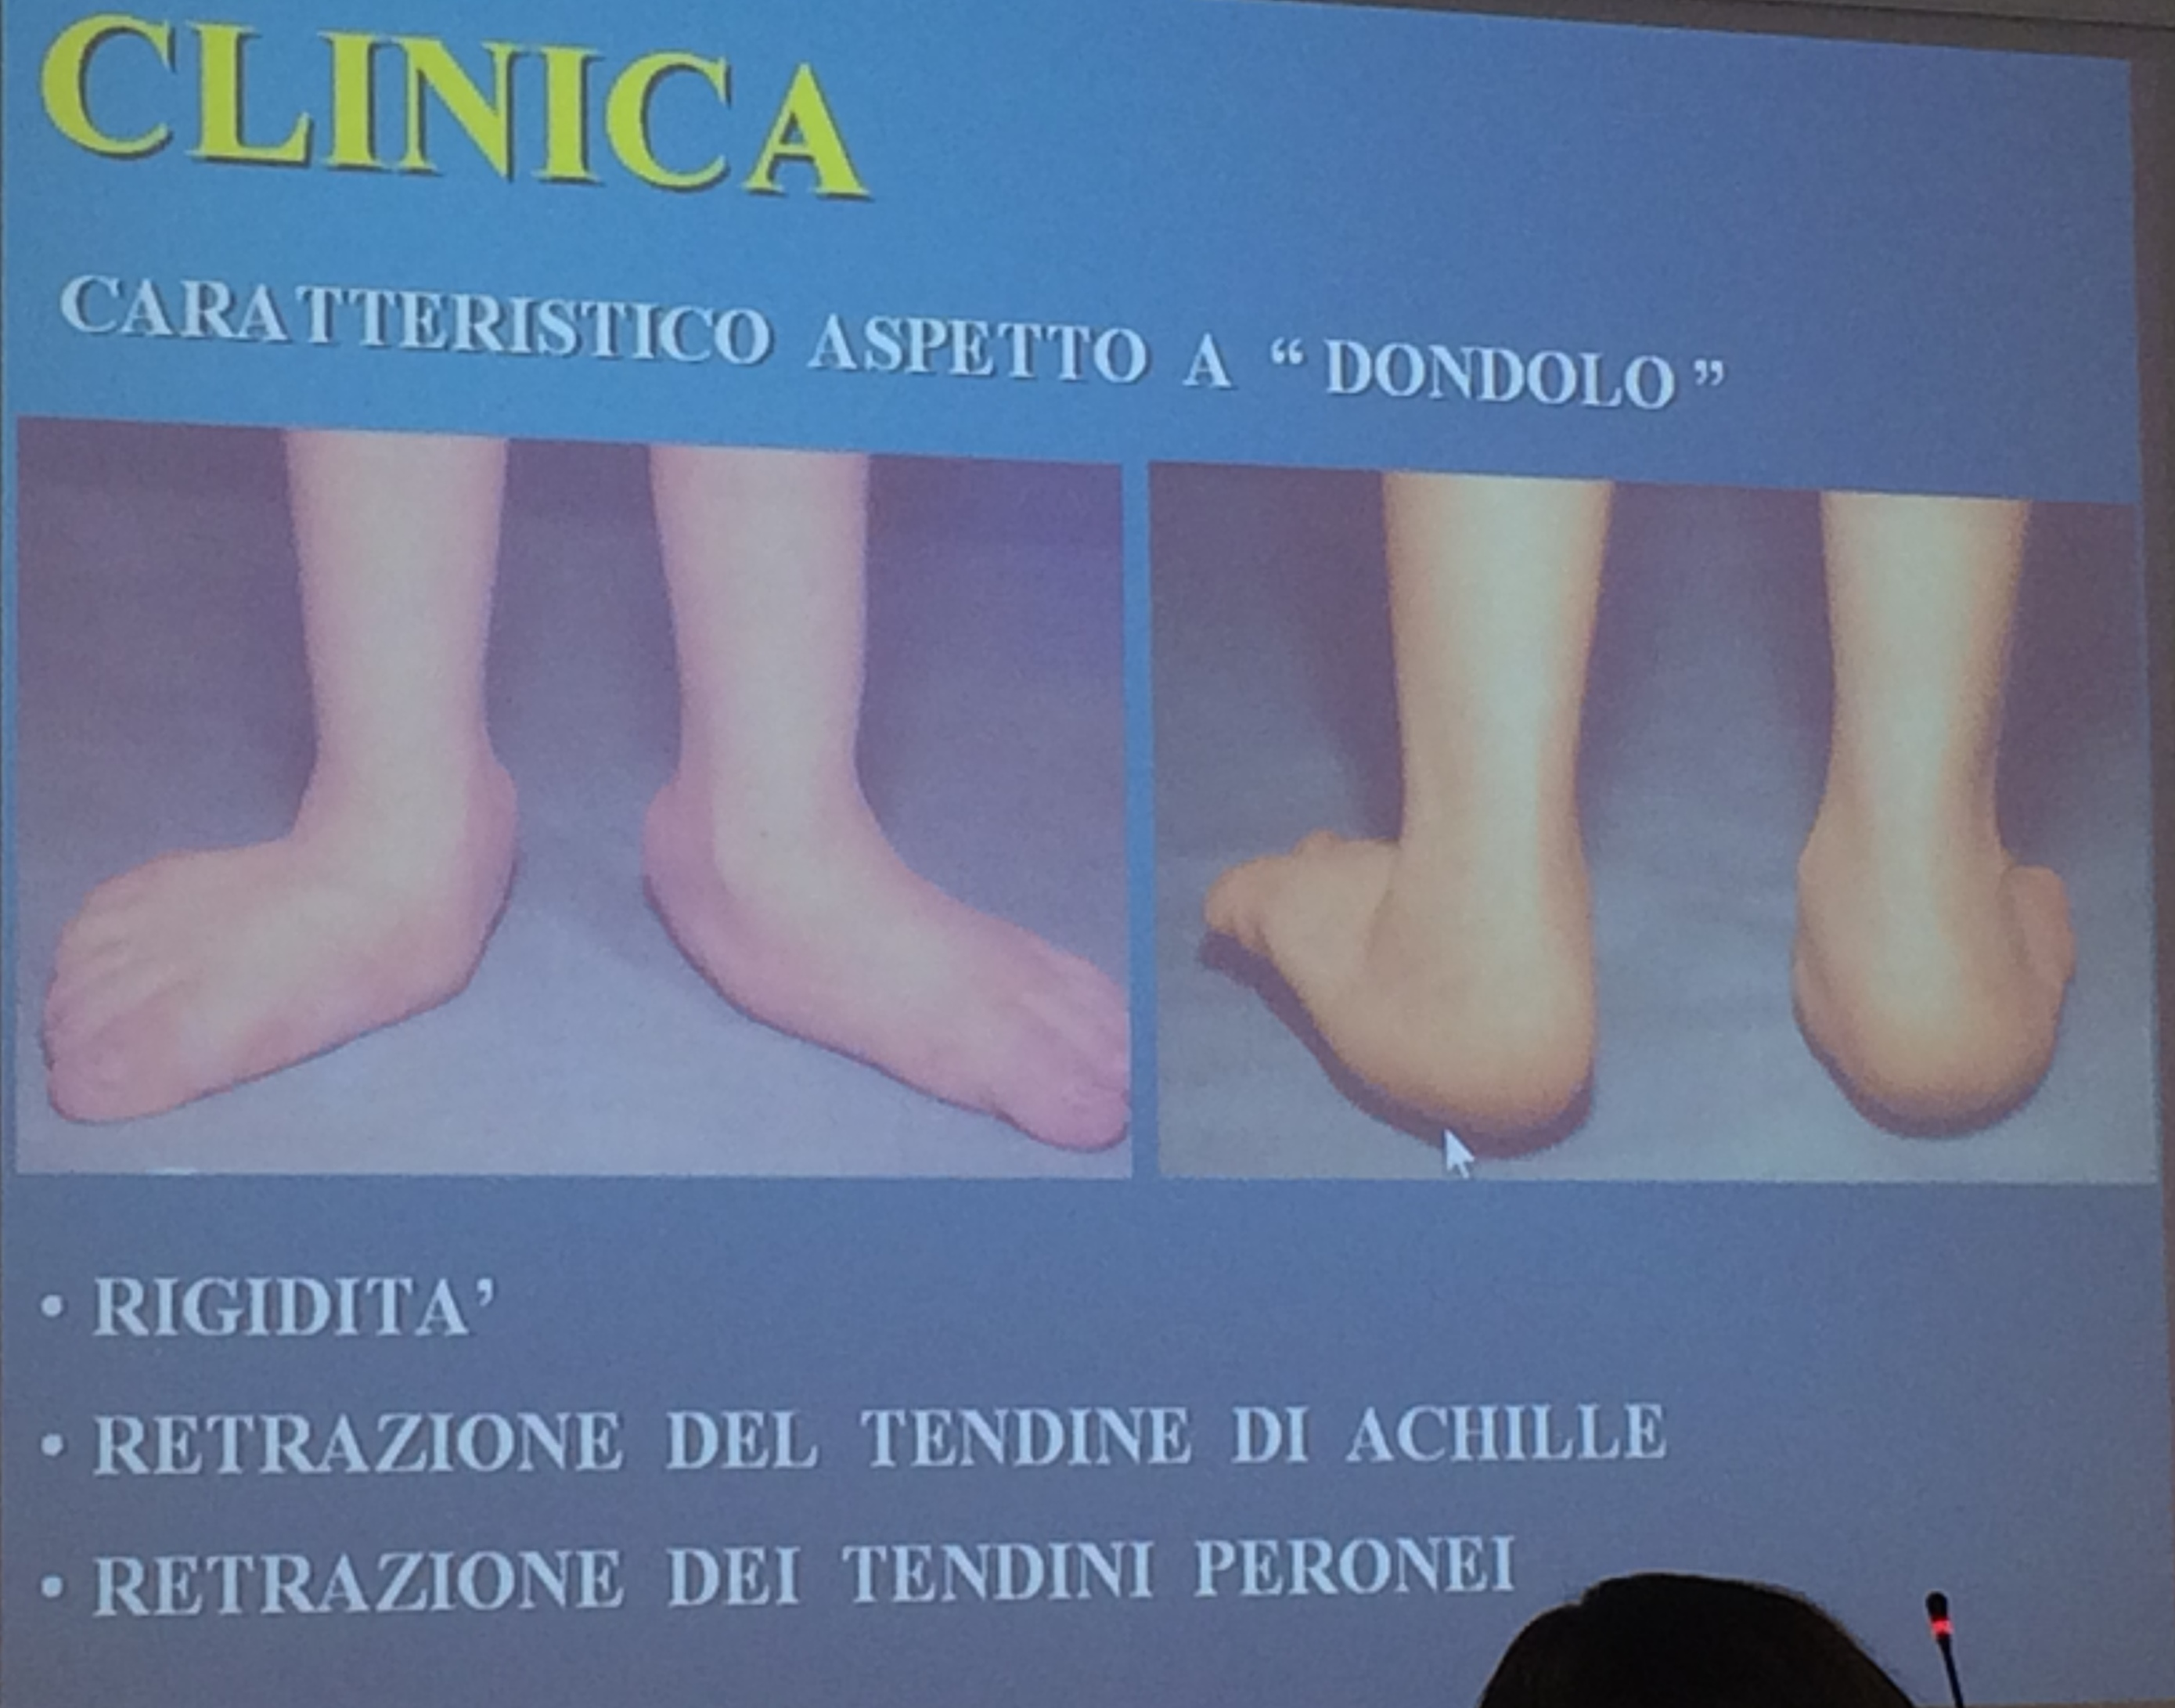
\includegraphics[width=3.39583in,height=3.00000in]{media/image10.jpeg}

\begin{itemize}
\item
  Radiografia
\end{itemize}

\begin{itemize}
\item
  Rx del polso standard antero-posteriore e latero-laterale: non sempre
  permettono di fare diagnosi
\item
  Rx con proiezione specifica per lo scafoide: proiezione
  postero-anteriore con polso deviato ulnarmente. Questa proiezione
  permette la diagnosi \emph{perché il movimento di deviazione ulnare
  tende a diastasare, allontanare e quindi far vedere meglio un
  eventuale presenza di una rima di frattura a livello dello scafoide}
\end{itemize}

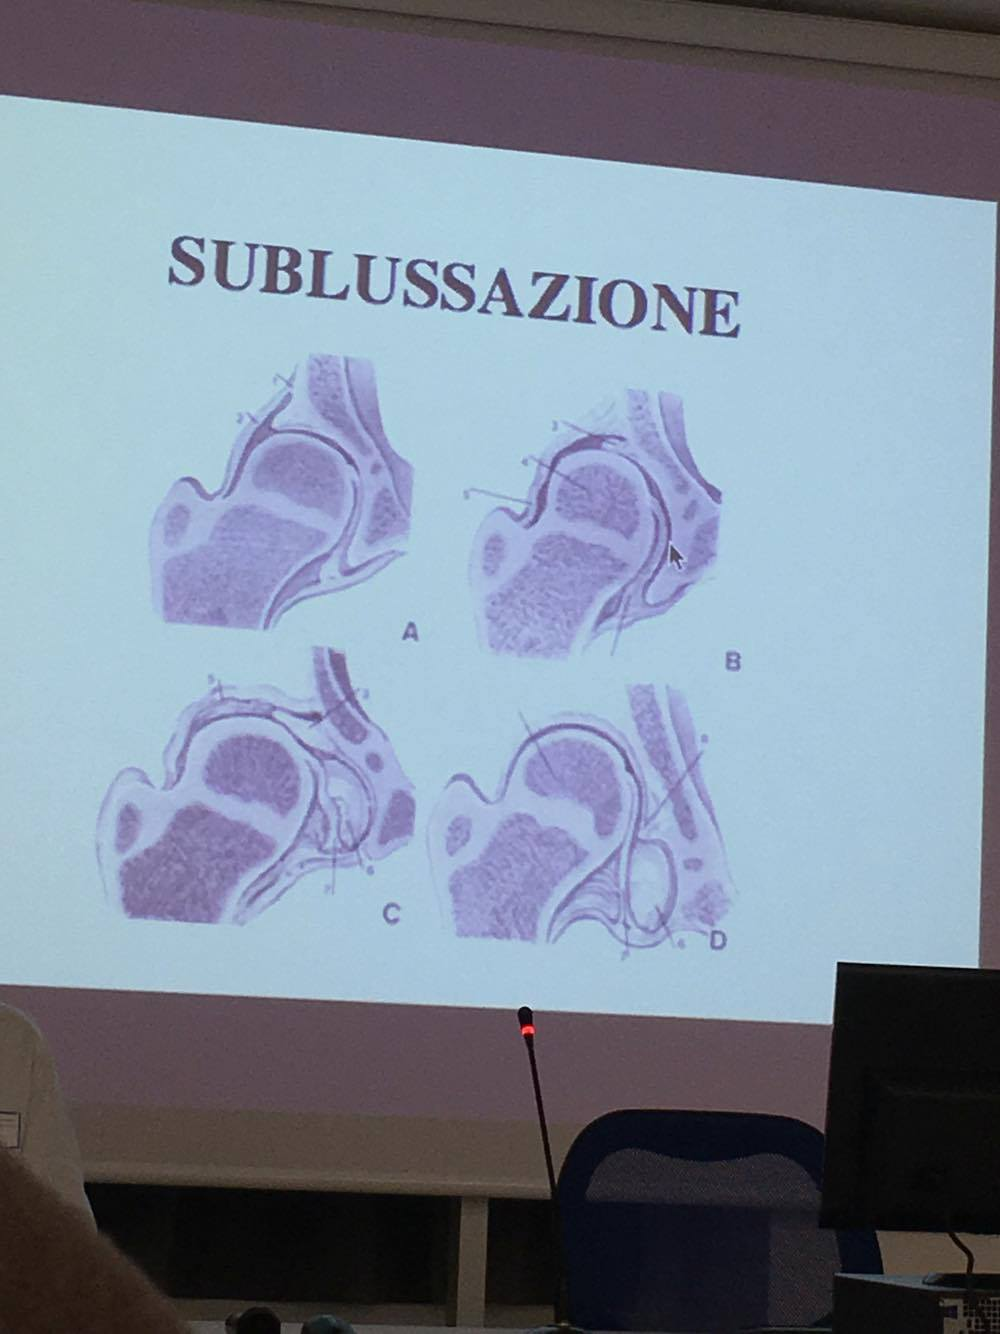
\includegraphics[width=3.90625in,height=2.93750in]{media/image11.jpeg}

\begin{quote}
Nella prima immagine si può vedere il polso in posizione
antero-posteriore normale; nella seconda immagine si vede il polso in
deviazione ulnare che tende a diastasare e a mettere in evidenza la
frattura.

NB: Molto spesso nelle prime radiografie la frattura dell'osso scafoide
non si vede! \emph{Perciò se si ha un sospetto clinico importante, con
dolore importate, un approccio potrebbe essere quello di
\emph{immobilizzare temporaneamente l'articolazione per una settimana}}
con un tutore o con una stecca gessata. Dopo 7-10 giorni si toglie e si
fa una rivalutazione e se il paziente ha ancora dolore si procede con
un'altra radiografia o ancor meglio con una TAC con tagli specifici
sullo scafoide che nella quasi totalità dei casi mette in evidenza la
frattura. Non è raro misconoscere la frattura dello scafoide \emph{vuoi
perché il paziente tende a sottovalutare il dolore o vuoi perché a volte
gli esami non la mettono in evidenza.} In questo caso il paziente si
ripresenta dopo 4-5 mesi con un dolore cronico a livello del polso, si
fa una Rx e si mette in evidenza non più una frattura dello scafoide
bensì \emph{una pseudoartrosi dello scafoide.}
\end{quote}

\end{document}

\section{Frattura dello scafoide}

Le fratture dello scafoide sono fratture un po' particolari: lo scafoide è un osso \emph{quasi completamente ricoperto da cartilagine (ad eccezione dei punti di inserzione dei legamenti)} con una
\emph{vascolarizzazione retrograda di tipo terminale}. Per queste due ragioni fratture di quest'osso guariscono con maggiore difficoltà.

La \textbf{prognosi} di guarigione dipende da diversi fattori:

\begin{itemize}
\item
  \textbf{Sede della lesione:} le fratture del polo prossimale guariscono con maggiore difficoltà, rispetto a quelle del terzo medio e del polo distale.
\item
  \textbf{Velocità della diagnosi:} molto spesso non sono diagnosticate immediatamente, ma a distanza di due/tre settimane, anche un mese, e non attraverso la radiografia normale, ma attraverso TAC (\emph{in questo caso la frattura può essere già andata incontro ad evoluzione in pseudoartrosi).}
Molto spesso non vengono neanche studiate: il paziente ha dolore in corrispondenza della tabacchiera anatomica, ma non va dal medico. A
distanza di sei mesi, un anno il dolore persiste, viene fatto un Rx e si vede così una frattura non diagnosticata, che è andata incontro a pseudoartrosi.
\item
  \textbf{Caratteristiche del paziente:} più o meno giovane, più o meno attivo.
Molto importanti sono anche le \emph{comorbilità}, che possono influenzare di base una normale guarigione della frattura.
I pazienti fumatori, i pazienti con problematiche internistiche, come diabete, ipertensione, ipertiroidismo vanno incontro a una guarigione più lenta.
\item
  \textbf{Adeguatezza del trattamento:} se si tratta incruentemente (ossia con un gesso) una frattura che dovrebbe essere operata, il risultato sarà peggiore.
Allo stesso tempo anche un intervento chirurgico non adeguato può influenzare negativamente la prognosi.
\end{itemize}

In più del 95\% dei casi questo tipo di fratture dei casi vengono trattate incruentemente con l'applicazione di un apparecchio gessato.
È importante ricordare che in ortopedia molto spesso \emph{i segni clinici di consolidazione}, ossia una riduzione della sintomatologia dolorosa, \emph{precedono i segni radiografici}.
\\\\
\emph{Epidemiologicamente, le fratture dello scafoide carpale sono fratture che si riscontrano nel \emph{giovane adulto}, con una prevalenza per il \emph{sesso maschile}, ed in una bassa percentuale dei casi (\textbf{2-3\%}) può essere \emph{bilaterale}, interessando prevalentemente il lato dominante del corpo, e nell'85\% dei casi sono
lesioni isolate, mentre nel restante 15\% dei casi sono associate ad altre lesioni della mano e del polso (ad esempio fratture del radio o lesioni dei legamenti intercarpali).}
\\\\
\emph{Il meccanismo traumatico alla base è in genere collegato con\emph{traumi in cui la mano viene  appoggiata in modo particolare, ossia quando c'è una caduta sul palmo della mano in iperestensione}: questo movimento fa sì che il corpo dello scafoide si incunei in corrispondenza della corrispondente superficie articolare del radio, così che si
sviluppa una sorta di meccanismo a leva che causa la frattura dello scafoide.}

\begin{figure}[!ht]
\centering
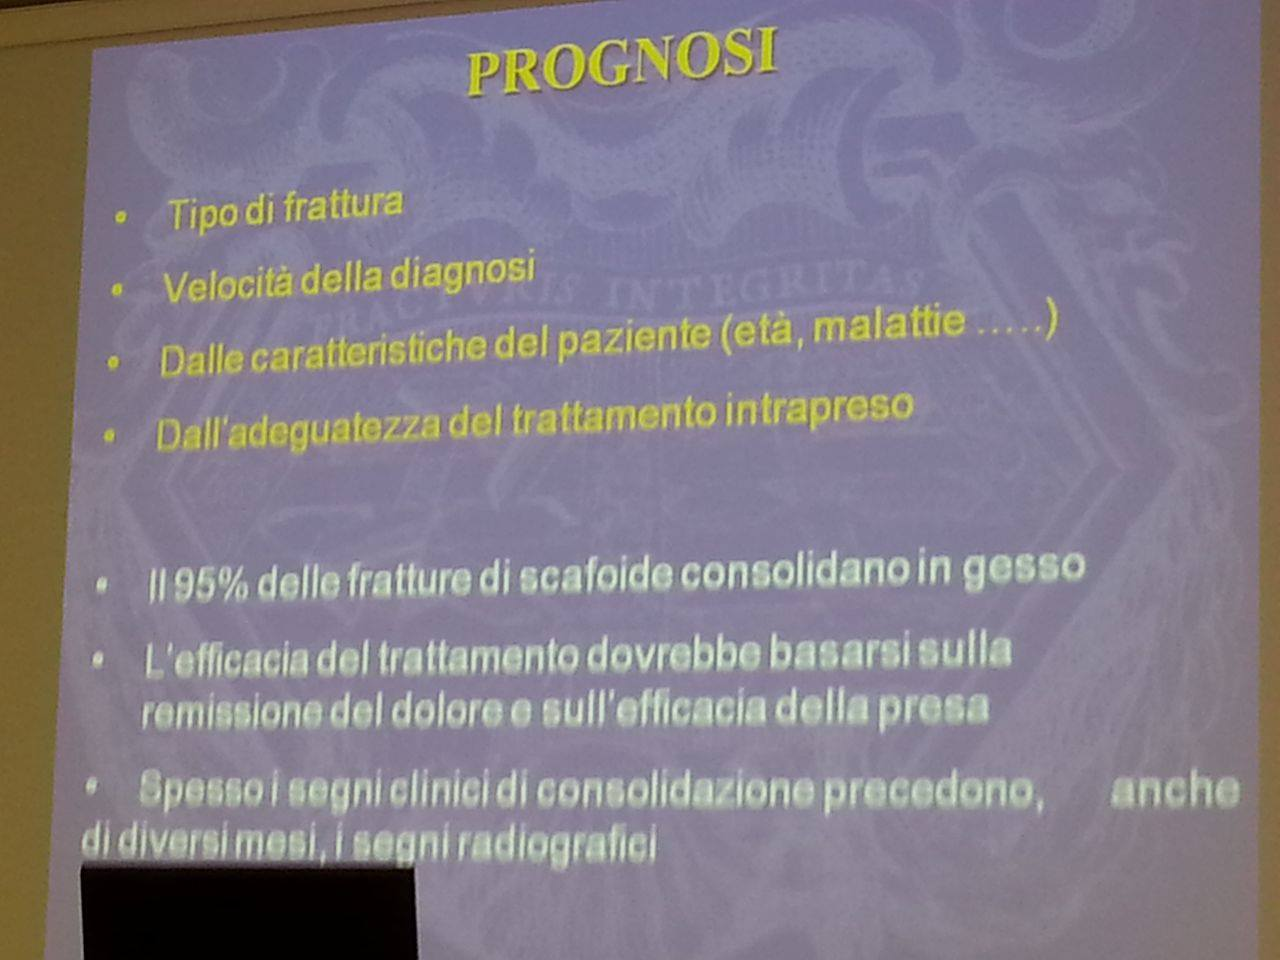
\includegraphics[width=0.5\textwidth]{004/image1.jpeg}
\end{figure}

\textbf{Le fratture dello scafoide posso essere divise in due tipi:}

\begin{itemize}
\item
  \emph{fratture a prognosi favorevole}: fratture \textbf{composte} e che interessano \textbf{polo distale e terzo medio} dello scafoide.
Nella maggior parte dei casi questo tipo di fratture guariscono con un trattamento incruento:
\begin{itemize}
\item
  in passato si faceva un gesso lungo \textbf{brachio-metacarpale con primo dito incluso} (gomito flesso a 90\textsuperscript{o} fissato), che dopo un mese veniva sostituito con un gesso più corto.
\item
  oggi si preferisce invece fin da subito un gesso più corto, \textbf{antibrachio-metacarpale}, cioè dalla fine dell'avambraccio fino ai metacarpi con primo dito incluso. Il gomito risulta libero.
\end{itemize}
Questo apparecchio gessato viene tenuto per più tempo rispetto a quelli applicati per altri tipi di frattura, proprio perché lo scafoide tende a
guarire più lentamente. Quindi se di solito un gesso di polso viene tenuto per 30-35-40 giorni, un gesso di scafoide rimane circa venti giorni in più.

Una volta rimosso il gesso, si fa una \emph{lastra di controllo}: si controlla che la frattura non si sia scomposta, si vede se ci sono iniziali segni di consolidazione anche radiografica (formazione di
\textbf{callo osseo}) e in un secondo tempo si provvede a fare della fisioterapia e della riabilitazione.

\begin{figure}[!ht]
\centering
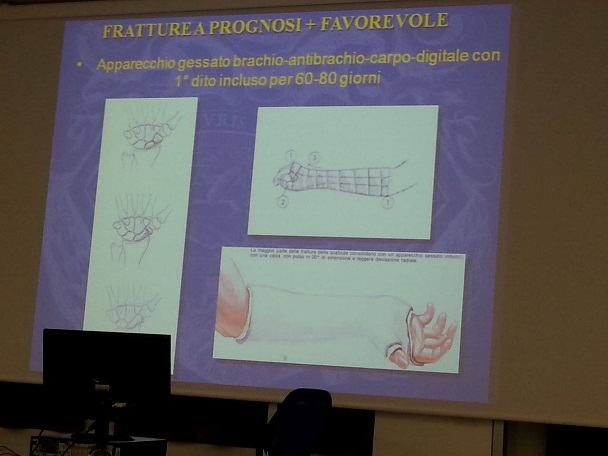
\includegraphics[width=0.5\textwidth]{004/image2.jpeg}
\end{figure}

\begin{figure}[!ht]
\centering
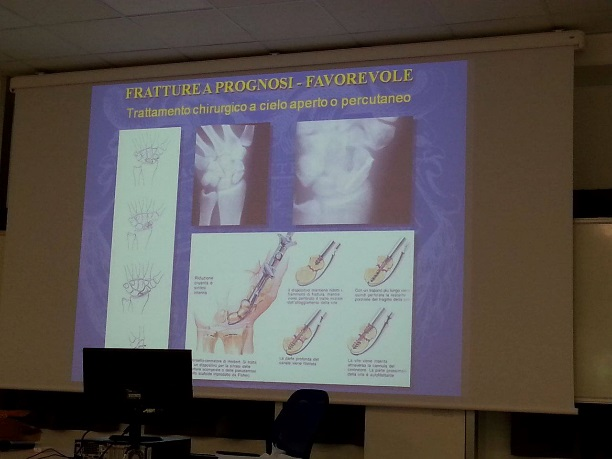
\includegraphics[width=0.5\textwidth]{004/image3.jpeg}
\end{figure}

\item
  \emph{Fratture a prognosi sfavorevole}: fratture \textbf{scomposte} di qualsiasi segmento e quelle del \textbf{polo prossimale}.

Di solito sono trattate chirurgicamente: si esegue una \textbf{sintesi}, ossia una stabilizzazione della frattura previa riduzione, con una vite
in compressione. La vite può essere applicata \emph{a cielo aperto} (si taglio, si espone la frattura, si riduce e poi si fa la sintesi con una
vita) o in modo \emph{percutaneo}, sfruttando un filo guida per inserire la vite all'interno dello scafoide attraverso delle piccole incisioni.
\end{itemize}

Questo in linea di massima è il protocollo terapeutico delle fratture
dello scafoide.

\begin{figure}[!ht]
\centering
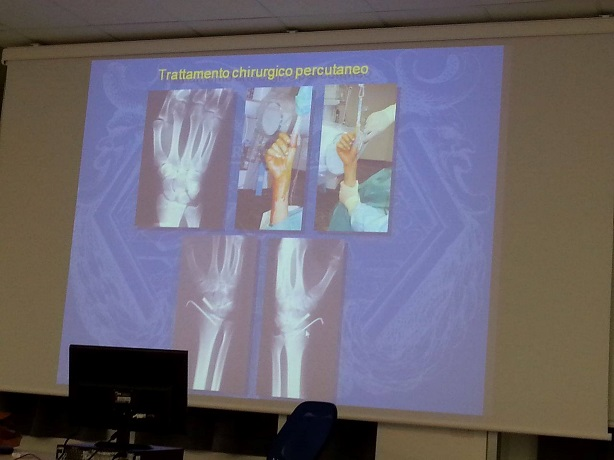
\includegraphics[width=0.5\textwidth]{004/image4.jpeg}
\end{figure}

\subsubsection{Complicanze}

Lo scafoide, come già detto, è un osso molto particolare. In caso di frattura va in contro ad una \textbf{crisi vascolare} e più facilmente può andare in contro a complicanze:

\begin{itemize}
\item
  \emph{Ritardo di consolidazione e pseudoartrosi} dello scafoide, per una mancata vascolarizzazione e un rallentamento o un blocco dei normali processi biologici che permettono la guarigione della frattura stessa.
\item
  \emph{Necrosi ossea ischemica}, se l'afflusso di sangue si riduce drasticamente.
\item
  \emph{Artrosi secondaria post-traumatica}, soprattutto se non viene fatta una riduzione anatomica. Essendo quest'osso ricoperto da cartilagine e articolato con il radio distale e le ossa del carpo, una mancata corretta riduzione può predisporre all'insorgenza di un'artrosi post traumatica più facilmente che in caso di fratture in altre sedi.
\end{itemize}

\begin{figure}[!ht]
\centering
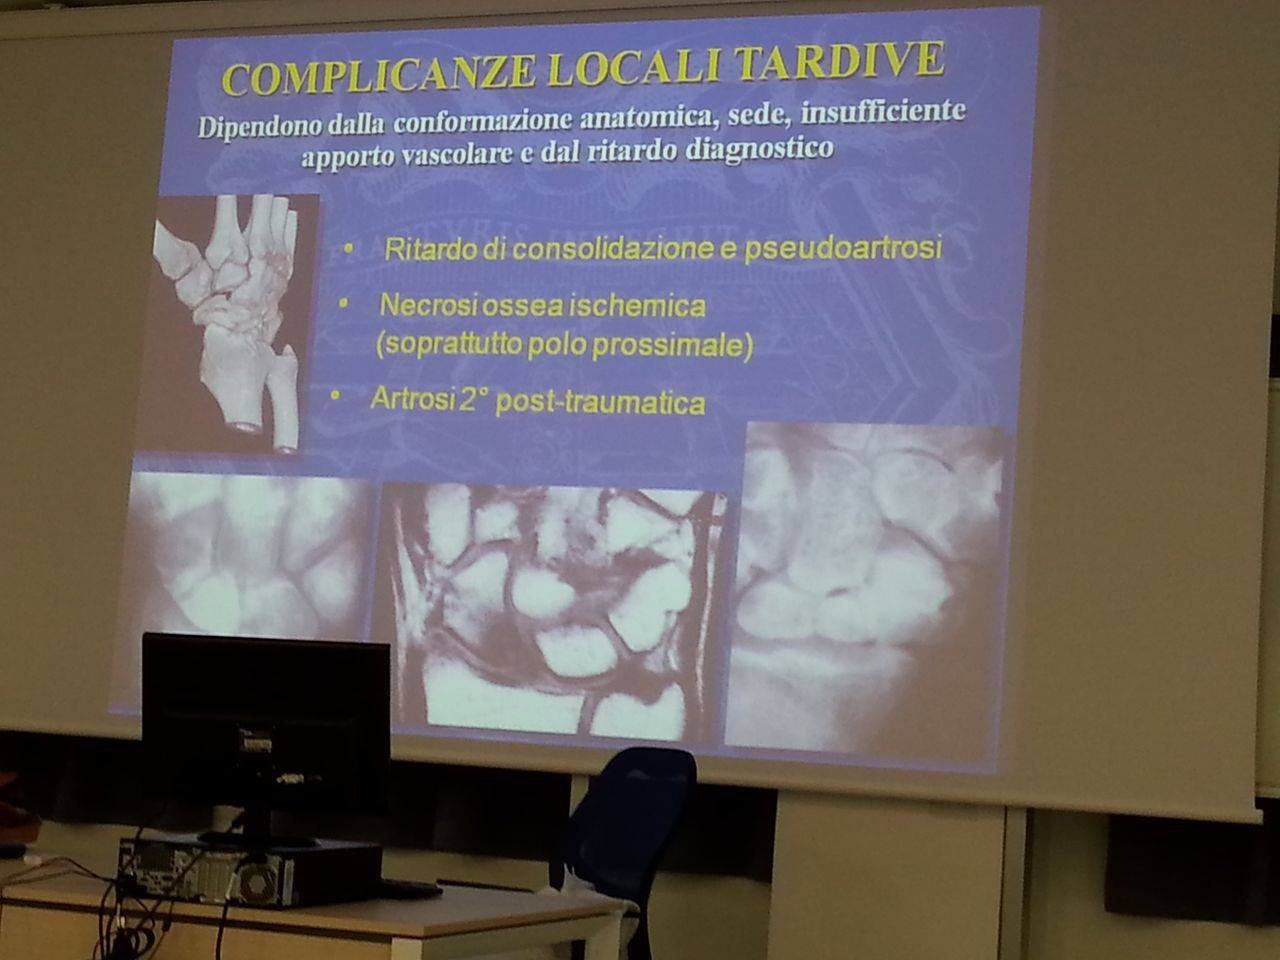
\includegraphics[width=0.5\textwidth]{004/image5.jpeg}
\end{figure}

Es (imm1): Rx di pseudoartrosi conseguente a mancata consolidazione di
una frattura del terzo medio dello scafoide: osso è bianco sul bordo e
si vede ancora la rima di frattura.

\begin{figure}[!ht]
\centering
\includegraphics[width=0.5\textwidth]{004/image6.jpeg}
\end{figure}

Es (imm2): RM con una necrosi del polo prossimale dello scafoide. 
\\\\
Di fronte a una pseudoartrosi di scafoide il trattamento è uguale a quello delle altre tipologie di pseudoartrosi.

La \textbf{psuedoartrosi} è una condizione di frattura che non è consolidata e non consoliderà assolutamente.

Per trattarla è necessario:

\begin{itemize}
\item
  aprire il focolaio di pseudoartrosi,
\item
  ripulirlo dal tessuto cicatriziale, connettivo, fibroso che si è formato,
\item
  ripristinare la conformazione anatomica normale,
\item
  far sanguinare l'osso, in modo tale che si riinizi un normale processo biologico di guarigione.
\end{itemize}

Si può inserire all'interno del focolaio di pseudoartrosi dell'osso, di solito prelevato da sé stessi, facendo un \emph{innesto osseo}. Si
preleva osso corticale e osso spongioso (ricco di cellule non differenziate, staminali, che possono stimolare la cascata della guarigione ossea) e il tutto viene messo all'interno del focolaio e poi
fissato attraverso dei fili metallici di Kirschner o delle viti.

Il miglior sito di prelievo è di solito la \emph{cresta iliaca}, dove è possibile prelevare grosse quantità di osso corticale e spongioso.
Durante il prelievo bisogna stare attenti a non ledere i nervi, come il nervo femoro-cutaneo laterale, che passa a cavaliere sopra la cresta
iliaca e che deve essere isolato e protetto per evitare dei neuromi dolorosi lungo il decorso di questo nervo.

Altri siti donatori sono: il radio distale, l'olecrano e la tibia
prossimale, anche se dal punto di vista quali-quantitativo la sede di
prelievo migliore è la cresta iliaca.

Per favorire la guarigione è quindi necessario:

\begin{itemize}
\item
  pulizia del focolaio,
\item
  la restitutio dell'anatomia normale,
\item
  stabilità conferita da viti o fili metallici
\item
  un buon apporto trofico e vascolare, dato da pulizia e apposizione di cellule ossee.
\end{itemize}

\section{Fratture del polso}

Le fratture del polso sono fratture molto frequenti:

\begin{itemize}
\item
  prevalentemente nella popolazione anziana, spesso legate ad osteoporosi.
\end{itemize}

\begin{itemize}
\item
  sono frequenti anche nel bambino, con fratture a legno verde
\item
  nei traumi ad alta energia nei giovani adulti.
\end{itemize}

Interessano \emph{l'epifisi ditale di ulna e del radio} e posso essere \emph{intra o extra-articolari} a seconda che la linea di frattura
interessi o meno la cartilagine articolare di radio e ulna.

\begin{figure}[!ht]
\centering
\includegraphics[width=0.5\textwidth]{004/image6.jpeg}
\end{figure}

Esistono \textbf{due tipi} di frattura:

\begin{itemize}
\item
  \textbf{Frattura di tipo COLLES:} la più frequente (85-90\%), soprattutto negli anziani, per un trauma da \emph{caduta sul palmo della mano}, con la mano atteggiata \emph{in iperestensione dorsale} (simile a modalità di frattura dello scafoide).
Vi è una scomposizione del radio distale e migrazione dorsale dei frammenti ossei. Può interessare anche il processo stiloideo dell'ulna.

Il reperto all'esame obiettivo è il cosiddetto \textbf{polso a dorso di forchetta}.

\begin{figure}[!ht]
\centering
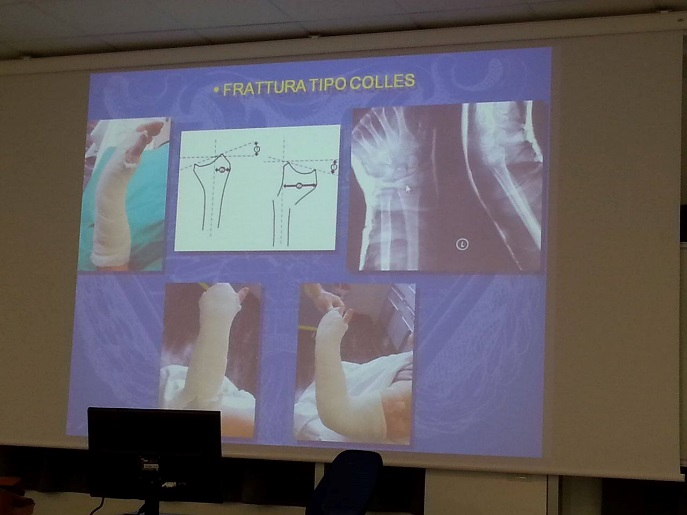
\includegraphics[width=0.5\textwidth]{004/image8.jpeg}
\end{figure}

\begin{figure}[!ht]
\centering
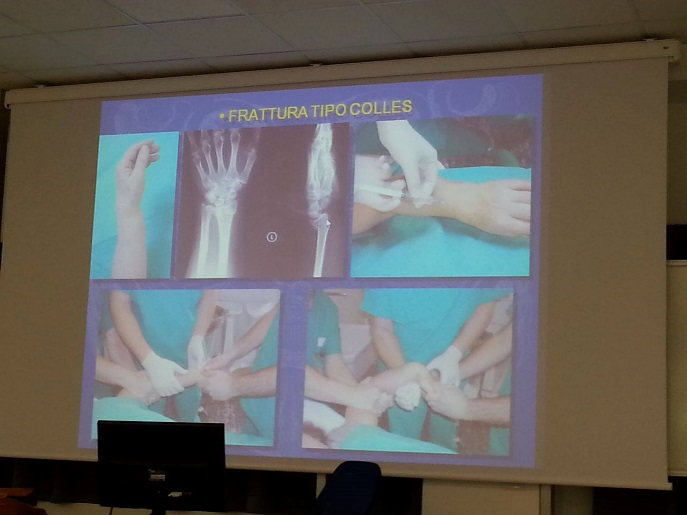
\includegraphics[width=0.5\textwidth]{004/image9.jpeg}
\end{figure}

\item
  \textbf{Fratture di tipo Goyrand:} sono fratture meno frequenti. Avvengo per \emph{caduta sul dorso della mano}, con un meccanismo eziopatogenetico opposto rispetto alle fratture di Colles.
La frattura si estrinseca nello stesso punto e il \emph{radio distale si scompone volarmente}, verso il palmo della mano.

\begin{figure}[!ht]
\centering
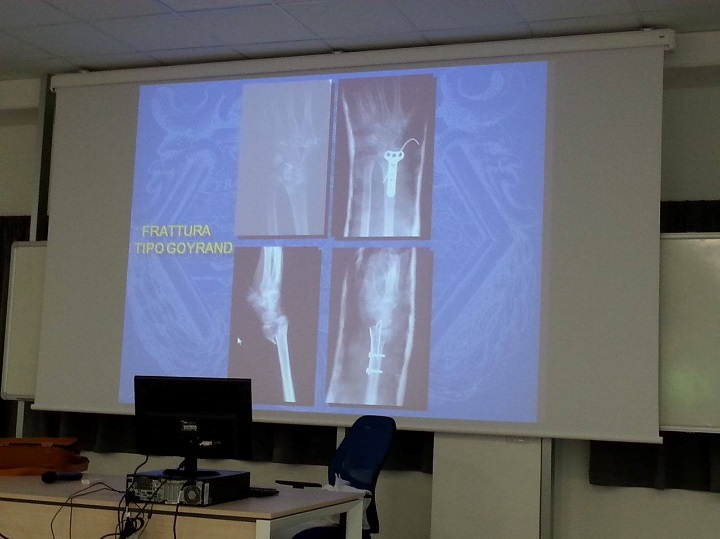
\includegraphics[width=0.5\textwidth]{004/image10.jpeg}
\end{figure}

\end{itemize}

\subsubsection{Trattamento}

Nel caso di fratture del polso, in PS bisogna sempre fare un \emph{tentativo di riduzione} in anestesia locale, a cui segue l'applicazione di un \emph{apparecchio gessato}.

Il gesso viene subito controllato con \textbf{radiografia}, per verificare che la riduzione sia efficace o meno. Devono essere
controllate radiologicamente in gesso dopo 7, 14 e a volte anche 21 giorni dall'evento. Questo perché questi tipi di fratture soprattutto (ma in realtà ogni tipo di frattura trattata con il gesso), possono, in questa sequenza temporale, andarsi a \textbf{scomporre}, perdendo la riduzione.

Questo avviene perché il segmento immobilizzato, sgonfiandosi, può non essere ben contenuto nel gesso e i micromovimenti che si vengono a creare determinano la perdita della riduzione.

In linea di massima nel momento in cui si perde una riduzione, si dà un'\emph{indicazione chirurgica}. La \textbf{perdita della riduzione} è indice di una \textbf{frattura instabile} ed è quindi, soprattutto nel giovane, indicato un intervento chirurgico.

A volte negli individui anziani, che mal sopporterebbero un intervento chirurgico, si può provare a rifare la riduzione.

Le fratture di \emph{tipo Goyrand} sono di solito \emph{più difficili da ridurre} e molto più frequentemente vanno incontro ad un intervento
chirurgico.

Questo di solito prevede una \textbf{riduzione} e \textbf{osteosintesi a cielo aperto} con placche e viti, a volte anche associato a fili metallici percutanei.

In casi ancora più selezionati, come nelle \emph{fratture esposte} e nelle \emph{fratture pluriframmentarie} del radio distale, dove non si
riesce a ridare stabilità con placche e viti, può essere indicato utilizzare uno \textbf{stabilizzatore esterno con distrazione}.

Viene applicato con due fiches a livello del metacarpo e due fiches in corrispondenza della metafisi distale del radio: la distrazione fa sì
che i legamenti radio-carpici, venendo stirati, tendano a ridurre a poco a poco la frattura.

Viene sfruttato il principio della \emph{legamentotassi}, ossia la trazione legamentosa determina una riduzione non anatomica, ma comunque
soddisfacente, della frattura.

Al fissatore esterno può anche essere associato l'uso di fili metallici, \emph{fili di Kirschner} \emph{percutanei}.

Il fissatore esterno viene mantenuto per almeno due mesi. Dopo un mese può essere \textbf{dinamizzato}, cioè rimane in distrazione, ma può essere permesso il movimento.

\section{Altre lesioni traumatiche della mano}

\subsection{MALLET FINGER}

Il MALLET FINGER (o dito a martello) si verifica quando si riceve un urto direttamente sull'estremità distale del dito e \emph{l'ultima falange assume un deformità a martello} (di solito giocando a basket,
pallavolo, calcio).

\begin{figure}[!ht]
\centering
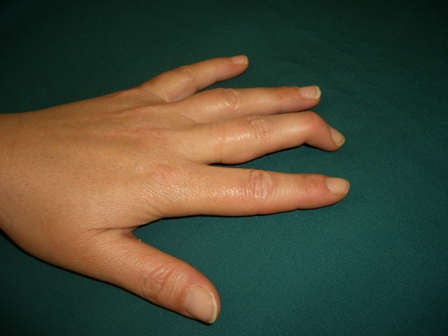
\includegraphics[width=0.5\textwidth]{004/image11.jpeg}
\end{figure}

Un deformità a martello può essere dovuta a due cause:

\begin{itemize}
\item
  una \emph{rottura sottocutanea dell'estensore del dito}, che di solito di inserisce a livello della falange distale
\item
  \emph{un'avulsione del tendine} che stacca l'osso sempre a livello della falange distale.
\end{itemize}

Quando arriva al PS un paziente con un dito a martello bisogna subito
fare un RX per vedere che sotto non ci sia una frattura della falange
distale.

\begin{itemize}
\item
  Il dito a martello associato a una frattura si chiama \textbf{lesione di Segond}.
\item
  Il dito a martello non associato a frattura si chiama semplicemente \textbf{rottura sottocutanea dell'estensore del dito a livello della falange distale}.
\end{itemize}

\subsubsection{Trattamento}

\begin{itemize}
\item
  Qualora vi sia solo una lesione a livello dell'estensore il trattamento è solitamente incruento e consiste nell'applicazione di una \textbf{stecca di Zimmer} o in plastica o metallica, che \emph{mantiene il dito iperesteso} all'interfalangea distale.
Ciò permette al tendine immobilizzato di cicatrizzare.
L'immobilizzazione deve essere mantenuta almeno 50-55 giorni.
Ogni tanto il paziente può togliere la stecca, con l'accortezza di mantenerlo iperesteso (o appoggiandolo sul tavolo o con l'altra mano).


Nel momento in cui la stecca viene tolta progressivamente il paziente può iniziare la \textbf{fisioterapia} per riacquisire l'articolarità.

Bisogna informare il paziente, che verosimilmente un po' di flessione dell'ultima falange rimarrà alla rimozione della stecca, ma anche se dal punto di vista estetico non sarà bellissima, dal punto di vista funzionale vi sarà un completo recupero.

\item
  Qualora invece siano associate delle fratture (lesione di Segond) bisogna valutare quanto \emph{osso} risulta essere \emph{avulso}, osservando una proiezione radiografica laterale.

Se il pezzo d'osso è superiore al 25\% dell'altezza del dito stesso, il trattamento è di solito chirurgico e consiste nella \textbf{reinserzione del frammento} nella propria sede.

Può essere fatto con microviti o fili metallici.

Si cerca comunque di evitare l'intervento chirurgico, perché si tratta di una zona cutanea molto delicata e la ferita può fare fatica a guarire
\end{itemize}

\subsection{LESIONE DI STENER}

La LESIONE DI STENER è la \emph{rottura del legamento collaterale ulnare in corrispondenza della prima articolazione metacarpo-falangea} della
mano.

Quest'articolazione è stabilizzata, oltre che dalla capsula articolare, da due legamenti: il legamento \textbf{collaterale ulnare} e il legamento \textbf{collaterale radiale}.

\begin{figure}[!ht]
\centering
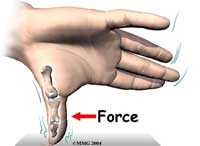
\includegraphics[width=0.5\textwidth]{004/image12.jpeg}
\end{figure}

Quello ulnare è molto importante perché garantisce la presa di forza della mano.

Si rompe soprattutto in ambito sportivo: per esempio sciando, nel tennis quando il dito rimane incastrato nella racchetta o negli incidenti in moto, quando il dito rimane vincolato al freno o all'acceleratore.

I pazienti presentano \textbf{dolore} e \textbf{tumefazione} localizzata e la manovra in stress radiale determina dolore e sensazione manuale di instabilità. Il dolore può essere molto forte e queste manovre posso quindi essere fatte iniettando un po' di anestetico locale.

Questa sensazione manuale di \textbf{instabilità} può essere confermata attraverso delle radiografie in stress bilaterali, fatte da un bravo tecnico radiologo.

Le radiografie mettono in evidenza l'apertura di questa articolazione rispetto alla controlaterale.

\subsubsection{Trattamento}

In un paziente giovane, attivo, con difficoltà della forza di presa in acuto deve essere trattato \textbf{chirurgicamente} (non immediatamente,
ma nel giro di 3-4-5 giorni).

Si taglia, si scosta il ramo sensitivo del nervo radiale, per evitare di lesionarlo e si riattacca il legamento con un'ancoretta a livello della falange (sede più tipica di rottura).

Le lesioni sono nella maggior parte dei casi a livello della falange, più raramente a livello della testa del metacarpo e ancora più raramente lungo il suo decorso.

All'intervento segue \textbf{l'immobilizzazione} attraverso un \emph{apparecchio gessato} per il primo dito o un \emph{tutore} su misura per una ventina di giorni e poi una \textbf{rieducazione} di
almeno un mese e mezzo per recuperare la forza dei muscoli dell'eminenza tenar e la forza di presa.

\documentclass[]{article}
\usepackage{lmodern}
\usepackage{amssymb,amsmath}
\usepackage{ifxetex,ifluatex}
\usepackage{fixltx2e} % provides \textsubscript
\ifnum 0\ifxetex 1\fi\ifluatex 1\fi=0 % if pdftex
  \usepackage[T1]{fontenc}
  \usepackage[utf8]{inputenc}
\else % if luatex or xelatex
  \ifxetex
    \usepackage{mathspec}
  \else
    \usepackage{fontspec}
  \fi
  \defaultfontfeatures{Ligatures=TeX,Scale=MatchLowercase}
\fi
% use upquote if available, for straight quotes in verbatim environments
\IfFileExists{upquote.sty}{\usepackage{upquote}}{}
% use microtype if available
\IfFileExists{microtype.sty}{%
\usepackage{microtype}
\UseMicrotypeSet[protrusion]{basicmath} % disable protrusion for tt fonts
}{}
\usepackage[unicode=true]{hyperref}
\hypersetup{
            pdfborder={0 0 0},
            breaklinks=true}
\urlstyle{same}  % don't use monospace font for urls
\usepackage{graphicx,grffile}
\makeatletter
\def\maxwidth{\ifdim\Gin@nat@width>\linewidth\linewidth\else\Gin@nat@width\fi}
\def\maxheight{\ifdim\Gin@nat@height>\textheight\textheight\else\Gin@nat@height\fi}
\makeatother
% Scale images if necessary, so that they will not overflow the page
% margins by default, and it is still possible to overwrite the defaults
% using explicit options in \includegraphics[width, height, ...]{}
\setkeys{Gin}{width=\maxwidth,height=\maxheight,keepaspectratio}
\IfFileExists{parskip.sty}{%
\usepackage{parskip}
}{% else
\setlength{\parindent}{0pt}
\setlength{\parskip}{6pt plus 2pt minus 1pt}
}
\setlength{\emergencystretch}{3em}  % prevent overfull lines
\providecommand{\tightlist}{%
  \setlength{\itemsep}{0pt}\setlength{\parskip}{0pt}}
\setcounter{secnumdepth}{0}
% Redefines (sub)paragraphs to behave more like sections
\ifx\paragraph\undefined\else
\let\oldparagraph\paragraph
\renewcommand{\paragraph}[1]{\oldparagraph{#1}\mbox{}}
\fi
\ifx\subparagraph\undefined\else
\let\oldsubparagraph\subparagraph
\renewcommand{\subparagraph}[1]{\oldsubparagraph{#1}\mbox{}}
\fi

% set default figure placement to htbp
\makeatletter
\def\fps@figure{htbp}
\makeatother


\date{}

\begin{document}

Morbo di Dupuytren

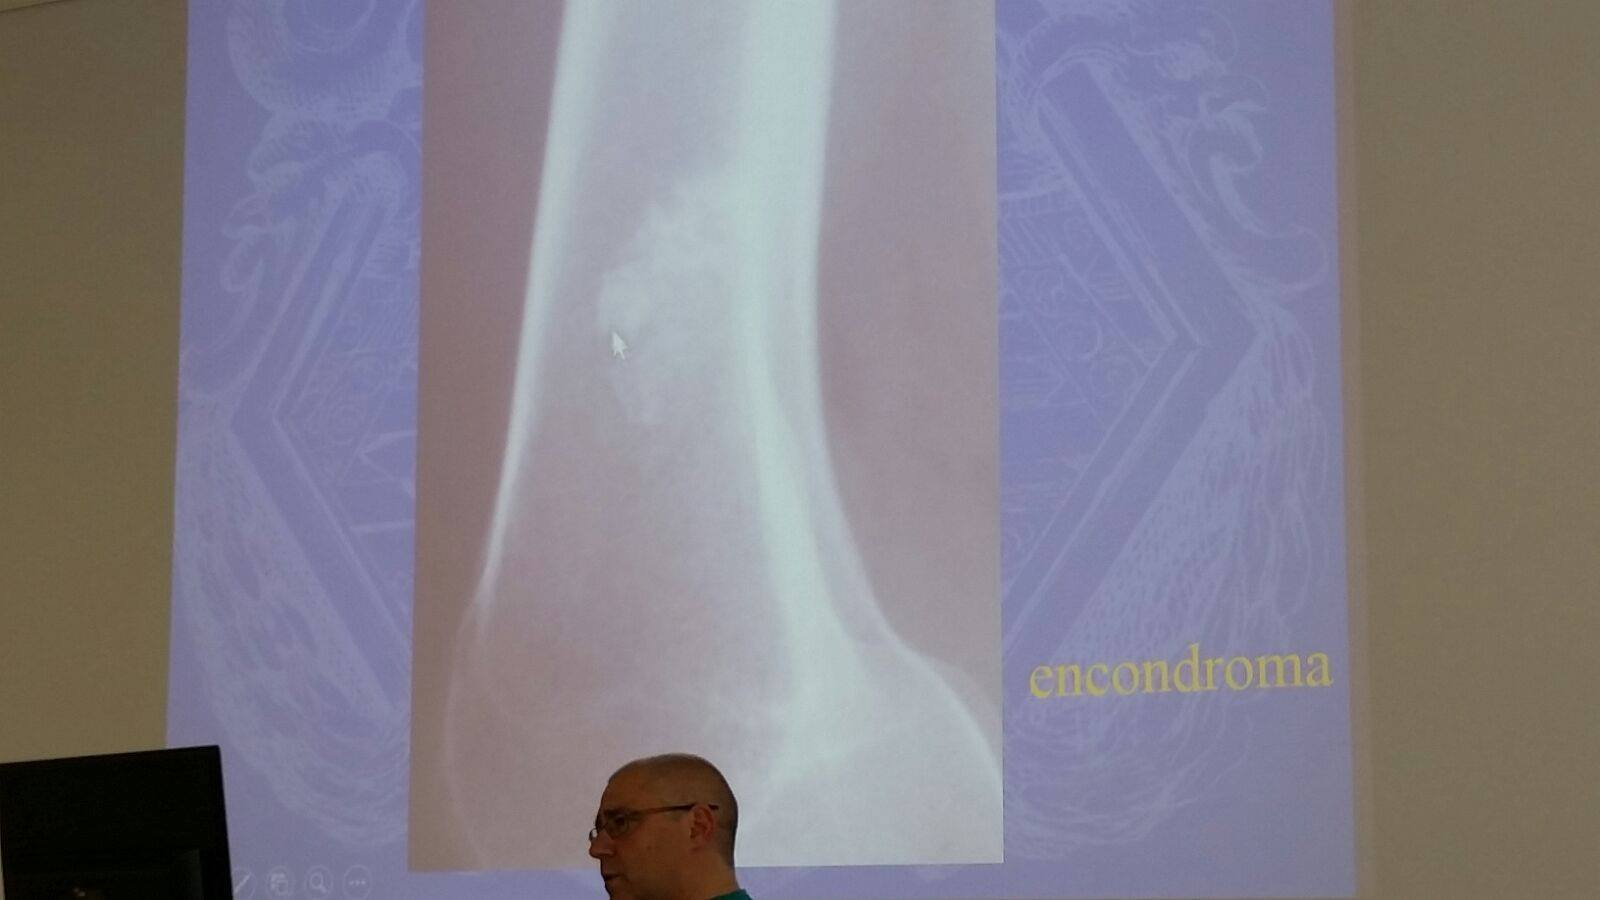
\includegraphics[width=4.02292in,height=2.24028in]{media/image1.jpeg}Il
morbo di Dupuytren è una patologia più frequente negli \textbf{uomini}
che non nelle donne, la cui eziopatogenesi non è ancora conosciuta in
maniera approfondita (E' una malattia degenerativa che coinvolge
fibroblasti e miofibroblasti, dovuto ad un primitivo danno vascolare
(ischemia microvascolare), si assiste alla proliferazione dei
fibroblasti lungo linee di stress meccanico, con formazione di strutture
cordoniformi nella fascia palmare).

Può esserci una componente familiare ed alcuni hanno associato lo
sviluppo di questa patologia a lavori che comportano vibrazioni a
livello della mano (es utilizzo di martelli pneumatici), o da patologie
come diabete, alcolismo, o farmaci tipo "Gardenale" ecompare di solito
dopo i 40 anni.

È caratterizzata da un \emph{progressivo ispessimento e da una
progressiva retrazione delle bandelette dell'aponeurosi palmare} che
possono far retrarre e far flettere le dita sia in corrispondenza
dell'articolazione metacarpofalangea che dell'articolazione
interfalangea.

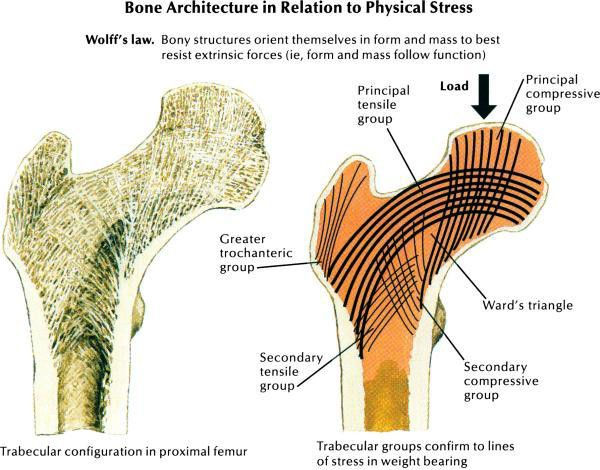
\includegraphics[width=3.03611in,height=2.02917in]{media/image2.jpeg}Generalmente
si presenta con la formazione di noduli fibrosi sottocutanei che
diventano poi cordoni sempre sottocutanei. La patologia colpisce
preferibilmente il \emph{quarto e il quinto raggio della mano} e meno
frequentemente i primi tre raggi. Spesso è bilaterale e si può
sviluppare anche alla pianta del piede. Bisogna sempre chiedere al
paziente se ha le stesse problematiche anche alla pianta del piede, come
\textbf{noduli o cordoni duri} che determinano la retrazione
dell'aponeurosi plantare. Nei maschi può essere associata a una
\emph{retrazione della tonaca albuginea del pene.} Queste complicanze
che riguardano piede e pene non sono frequenti ma devono essere tenute
in considerazione.

Diagnosi

La diagnosi è per questo tipo di patologia è essenzialmente clinica,
bisogna vedere la mano e palpare il nodulo o il cordone che si sente
molto bene in corrispondenza del palmo. La velocità di progressione da
nodulo a cordone e da dito esteso a dito flesso e a dito flesso
totalmente non è assolutamente prevedibile, può essere velocissima
oppure il paziente può restare stabile per anni senza avere nessun tipo
di retrazione. Molto spesso in ambulatorio arrivano degli stadi iniziali
di morbo di Dupuytren che noi non trattiamo chirurgicamente.

Trattamento

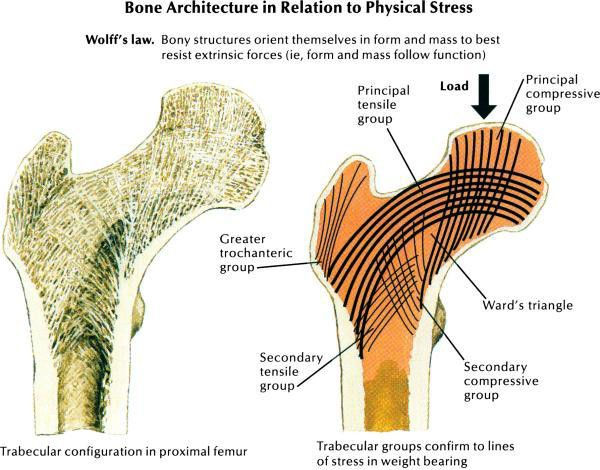
\includegraphics[width=2.60208in,height=3.40764in]{media/image3.jpeg} Il
trattamento iniziale infatti è di tipo astensionistico ed osservazionale
a domicilio; si dice al paziente di guardare se il nodulo diventa
cordone, se inizia a retrarsi e a piegarsi il dito, e in quel caso si va
verso un ipotesi chirurgica.

La chirurgia è nella maggior parte dei casi a cielo aperto e
l'intervento viene fatto possibilmente con occhiali da microchirurgia.
Si fanno delle incisioni curvilinee a zig zag al di sopra dei cordoni o
dei noduli, e si va a togliere l'aponeurosi retratta ossia quella
patologica \emph{( N.B. l'immagine a lato con i nomi delle incisioni è a
solo scopo illustrativo}).

L'intervento si chiama perciò di \textbf{aponeurectomia selettiva}
quindi:

\begin{itemize}
\item
  Anestesia generale o loco-regionale del braccio
\item
  Ricovero ospedaliero per 24\textasciitilde{}48ore;
\item
  Larga apertura,unica o multipla,delle dita e del palmo della mano per
  l'asportazione della
\end{itemize}

fascia palmare ispessita e retratta;

\begin{itemize}
\item
  Cicatrizzazione cutanea di 2settimane;
\item
  Riabilitazione di 1\textasciitilde{}2mesi;
\item
  Utilizzo di tutore notturno per le dita operate;
\item
  Sospensione del lavoro di 1\textasciitilde{}2mesi per i lavoratori
  manuali
\end{itemize}

In alcuni casi molto selezionati si potrebbe fare una
\textbf{aponeurectomia percutanea}, ossia con un ago viene tagliato il
cordone fibroso per recuperare l'estensione del dito è una tecnica
mini-invasiva, consiste nella sezione multipla della sclerosi
aponeurotica, ispessita e retratta, eseguita con un ago , abbiamo:

\begin{itemize}
\item
  Anestesia locale
\item
  Senza ricovero,in day-hospital;
\item
  Tecnica mini-invasiva,senza apertura delle dita e del palmo della
  mano: l'ago taglia in sotto-
\item
  cutaneo la fascia palmare retratta in diversi punti e quindi si
  allunga normalmente;
\item
  Nessun tempo di cicatrizzazione;
\item
  Minima riabilitazione;
\item
  Nessuna sospensione del lavoro;
\item
  Raramente si utilizzerà un tutore notturno.
\end{itemize}

Questa tecnica è, purtroppo, molto spesso dimenticata o non conosciuta
dagli specialisti, per cui troppi malati non possono beneficiarne.

Possono essere utilizzati anche dei \textbf{farmaci} (non in commercio
in Italia) che vengono iniettati nel sottocute e ``sciolgono'' il
cordone aponeurotico. Nella maggior parte dei casi però si interviene
chirurgicamente con l'aponeurectomia selettiva. I cordoni fibrosi
tendono ad inglobare i nervi digitali che danno la sensibilità alle
dita, quindi l'intervento di aponeurectomia si fa primariamente sui
nervi e poi sulle altre strutture, ossia devono essere prima isolati,
scollati e protetti i fasci vascolonervosi della mano, e poi viene tolto
il fascio stesso.

Come complicanza ci può essere una lesione vascolonervosa, ad esempio
del nervo digitale, perché scollando può essere tagliato o lesionato.
Altre complicanze presenti dopo questo intervento sono le recidive che
si suddividono in:

\begin{itemize}
\item
  \emph{recidive vere}, dovute al fatto che non viene tolta tutta
  l'aponeurosi patologica e di conseguenza si riforma un cordone che
  retrae. In questo caso bisogna riaprire e togliere l'aponeurosi
  patologica.
\item
  \emph{recidive false}, dovute ad una retrazione successiva
  all'intervento chirurgico e legata alla formazione di una cicatrice
  aberrante o di un \textbf{cheloide} che determina la retrazione del
  raggio e del dito che è stato operato. In questo caso, grazie alla
  chirurgia plastica, si possono fare interventi di allungamenti e
  plastiche a zeta per ritornare ad avere il dito esteso.
\end{itemize}

A volte arrivano in ambulatorio pazienti in uno stadio avanzato, ad
esempio anziani che riferiscono di aver sempre avuto un dito flesso e
che non ha dato alcun fastidio, ma solo qualche limitazione nei
movimenti quotidiani (es afferrare oggetti, mettere i guanti). In questo
caso c'è l'indicazione chirurgica, stiamo parlando però di persone che
hanno questa rigidità in flessione da anni, di conseguenza tutte le
strutture vascolo nervose si sono retratte e accorciate. Può capitare
che ridando la lunghezza e l'estensione giusta del raggio possano venire
stirati e rotti i nervi e ci possono quindi essere delle crisi
vascolari. In questi casi si può dire al paziente che si può fare un
tentativo per recuperare l'estensione, se vanno in crisi vascolare può
darsi che si debba amputare il dito. In alcuni casi estremi si
preferisce amputare subito piuttosto che fare il raddrizzamento e poi
eventualmente l'amputazione. Questo non è un intervento da anestesia
locale, ma viene fatto con un \textbf{anestesia plessica}. Di solito il
paziente resta ricoverato una notte e a seconda della gravità del morbo
di Dupuytren e di conseguenza del grado di retrazione in flessione delle
dita, il decorso post operatorio è più o meno facile.

Nel decorso post-operatorio di una forma iniziale:

\begin{itemize}
\item
  si fa un bendaggio,
\item
  si cura la cicatrice,
\item
  dopo 15 giorni si tolgono i punti,
\item
  infine si fa un trattamento della cicatrice che consiste in un
  massaggio desensibilizzante per far riassorbire l'ematoma,
\item
  recupero progressivo della mobilità.
\end{itemize}

Nei casi più gravi (quando c'è una flessione abbastanza importante prima
dell'intervento chirurgico):

\begin{itemize}
\item
  si associa il posizionamento di una stecca gessata in estensione per
  mantenere le dita dritte per i primi 15 giorni da tenere tutto il
  giorno,
\item
  alla rimozione dei punti può iniziare la fisioterapia per il recupero
  dell'articolarità e il trattamento fisioterapico della ferita,
\item
  si possono fare dei tutori su misura amovibili dorsali, ossia dalla
  parte opposta della ferita in estensione, che inizialmente vengono
  mantenuti negli intervalli tra le sedute fisioterapiche,
\item
  dopo 1 mese dall'intervento il tutore deve essere tenuto di notte per
  almeno 6-8 mesi dall'intervento.
\end{itemize}

Sindrome di De Quervain

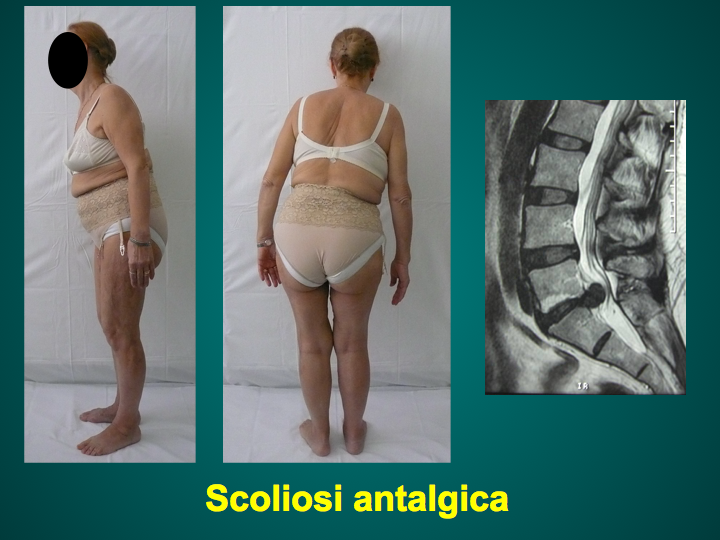
\includegraphics[width=2.44097in,height=1.74722in]{media/image4.png}Altra
patologia della mano abbastanza frequente è la sindrome di De Quervain
che per definizione è una \textbf{tenosinovite o tenovaginalite
stenosante} dei tendini:

\textbf{1}-\textbf{estensore breve }

\textbf{2-abduttore lungo del pollice}

tendini che attraversano il primo compartimento osteo-fibroso degli
\textbf{estensori}, presente sulla superficie dorsale del radio.

I tendini estensori decorrono a livello del radio distale in canali
osteo-fibrosi, che vanno a costituire i sei compartimenti degli
estensori

\begin{enumerate}
\def\labelenumi{\arabic{enumi}.}
\item
  Il primo compartimento è quello che interessa il morbo di De Quervain
  e al suo interno passano l‟estensore breve del pollice e l‟abduttore
  lungo del pollice;
\item
  Il secondo compartimento accoglie gli estensori radiali (breve e
  lungo) del carpo ;
\item
  Il terzo compartimento è quello dell‟estensore lungo del pollice;
\item
  Il quarto compartimento contiene l‟estensore comune delle dita e
  l‟estensore proprio dell‟indice;
\item
  Il quinto compartimento contiene l‟estensore proprio del V dito;
\item
  Nel sesto e ultimo compartimento passa l‟estensore ulnare del carpo.
\end{enumerate}

I tendini estensori passano attraverso queste strutture e sono ricoperti
dalle loro guaine sinoviali: quando si ha una compressione dei tendini
compresi nel primo compartimento si parla di morbo di De Quervain.

Se si abduce il primo dito si vede un tendine, questo è
\emph{l'estensore lungo del pollice}, se vi avvicinate verso il palmo
della mano a livello dell'articolazione del polso si sentono altri due
tendini o un cordone composto da quei tendini; questo è quello che
riguarda il morbo di De Quervain, ovvero l'estensore breve e l'abduttore
lungo. Tutti gli estensori a livello del dorso del polso sono contenuti
all'interno di canali osteofibrosi; la loro presenza permette che i
tendini scorrano al loro interno durante l'estensione del polso e non si
stacchino dall'osso. Non c'è quindi l'effetto corda d'arco. Quando i
tendini, per vari motivi (ad es per la degenerazione di una corda
tendinea o per un processo infiammatorio delle guaine peritendinee),
fanno fatica a scorrere all'interno di questi canali osteofibrosi, si
possono avere delle tendinovaginaliti stenosanti ed è il caso del morbo
di De Quervain. Questa patologia è più frequente nelle \textbf{donne}
,(Rapporto M:F 1:6) che non negli uomini, ed è correlata a quelle
\textbf{attività lavorative o ludiche} che comportano un estensione
continua del pollice, in particolare è caratteristica delle donne che
lavorano molto con le dita, che abbiano attività caratterizzate da
movimenti ripetitivi di abduzione radiale del pollice, con simultanea
inclinazione ulnare del polso. La fascia d'età più colpita coincide con
la quarta e quinta decade.

Clinica

Dal punto di vista clinico è presente un dolore elettivo a livello della
stiloide radiale,punto in cui decorrono i tendini sopracitati,
esacerbato dalla digitopressione e dalla estensione contro resistenza.
Ci può essere una tumefazione, e a volte può essere presente anche un
crepitio, legato al fatto che il tendine con la sua guaina rigonfia fa
fatica a scorrere e in questo canale si può saltuariarmente sentire un
\emph{crik-crok , se nel movimento di flesso-estensione del pollice, si
appoggiano le dita lungo il decorso del tendine, si possono sentire dei
piccoli ``sfrusciamenti'', causati della guaina del tendine che scorre.
La diagnosi è clinica e c‟è un test specifico: }

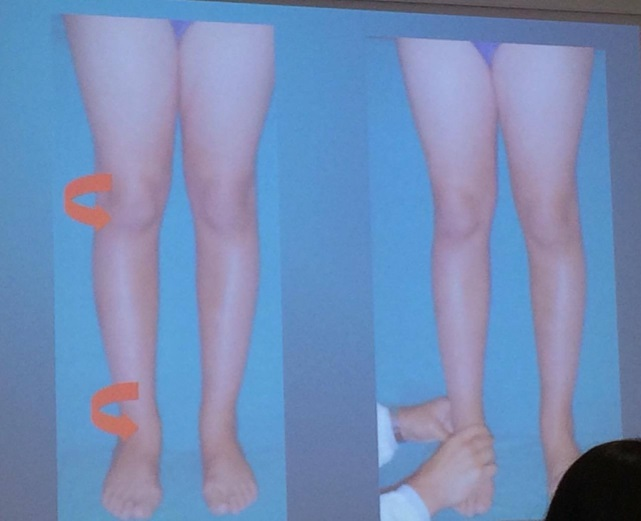
\includegraphics[width=4.22917in,height=2.02708in]{media/image5.jpeg}

Il \textbf{Test di Finkelstein} è un test specifico in cui si chiede al
paziente di mettere il pollice in questa posizione, di chiudere le altre
dita al di sopra del pollice e di inclinare ulnarmente il polso.
\emph{Questa inclinazione ulnare attiva o passiva fatta da un
esaminatore determina un dolore caratteristico a livello della stiloide
radiale} che si può irradiare lungo il decorso dei due tendini e dei due
ventri muscolari.

Diagnosi

La diagnosi è primariamente clinica, di solito per confermarla si
possono fare degli esami strumentali e in particolare uno studio
\textbf{ecografico} bilaterale dei polsi è sufficiente per mettere in
evidenza questa patologia,può mettere in evidenza un‟infiammazione dei
tendini interessati.

A volte è giusto fare anche una \textbf{radiografia} associata perchè
possono esserci delle protuberanze o delle esostosi della stiloide
radiale che possono favorire l'insorgenza di questa patologia,a volte ci
possono essere degli osteofiti della stiloide radiale che vanno a
comprimere i tendini, in tal caso il trattamento sarà chirurgico.

Trattamento

Il trattamento come sempre è di tipo conservativo; si possono usare dei

\begin{itemize}
\item
  \textbf{Tutori su misura} che mette a riposo l'articolazione e il dito
\end{itemize}

dell'articolazione del polso e del primo raggio.

\begin{itemize}
\item
  Il passaggio successivo, che ha un risultato positivo in una buona
  percentuale di pazienti (50-80\%), è quello di fare delle
  \textbf{infiltrazioni con corticosteroidi locali}, bisogna essere però
  in grado di andare con l'ago tra il tendine e il canale osteofibroso
  ed iniettare il cortisonico non dentro al tendine ma attorno ad esso(
  i corticosteroidi dovranno essere iniettati in zona peritendinea e non
  intratendinea, arrivando al di sotto della guaina che copre il
  tendine).
\end{itemize}

Procedura:

1-palpo il tendine;

\begin{quote}
2-inserisco l‟ago che arriva in profondità, deve superare la guaina
tendinea;

3- passivamente muovo il dito, se l‟ago ``sbandiera'' vuol dire che ho
punto il tendine, se invece rimane perpendicolare vuol dire il tendine
non è stato punto e posso iniettare.

4 L‟infiltrazione deve essere peritendinea, quindi devo superare la
guaina tendinea, ma non andare

dentro il tendine!
\end{quote}

\begin{enumerate}
\def\labelenumi{\arabic{enumi}.}
\item
  3-Qualora il trattamento conservativo non abbia successo si può fare
  un \textbf{trattamento chirurgico} che consiste nella
  \emph{liberazione del tendine dalla compressione} presente all'interno
  del canale osteofibroso interessato. Si fa quindi un intervento di
  \textbf{tenolisi}, di liberazione del tendine, che è svolto in
  anestesia locale e non prevede un ricovero, dopo qualche ora il
  paziente può tornare a casa. Di solito si preferisce fare non tanto un
  incisione longitudinale lungo il decorso dei tendini dei muscoli, ma
  piuttosto un \emph{incisione trasversale} centrata sulle pliche
  dorsali del radio in quanto darà una cicatrice molto più bella.
  Bisogna stare attenti nel fare il taglio trasversale in quanto c'è un
  ramo sensitivo del nervo radiale che passa a questo livello e che dà
  la sensibilità dorsale in tutta questa zona. Se tagliato o lesionato
  può dare ipoanestesia della zona interessata ma può anche causare dei
  neuromi dolorosi da amputazione del nervo. Questa patologia può essere
  mono o bilaterale, essendo però legata a prese di forza o movimenti
  ripetuti di solito interessa la mano dominante.
\end{enumerate}

Dito a scatto

Esiste un'altra patologia molto frequente che è nominata dito a scatto;
si tratta di una una \textbf{\emph{tenovaginite stenosante che interessa
i flessori delle dita}}. Lo scatto può essere causato da un
restringimento del canale oppure dal fatto che il tendine infiammato
faccia fatica a scorrere in corrispondenza della base del dito. Questa
stenosi si verifica in corrispondenza della \textbf{superficie volare
del palmo della mano a livello della testa dei metacarpi}, dove è
presente una struttura che è la prima puleggia circolare chiamata anche
\textbf{puleggia A1}.

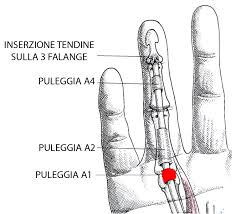
\includegraphics[width=3.24236in,height=3.77361in]{media/image6.png}

Il flessore superficiale si inserisce volarmente alla base della seconda
falange, il flessore profondo si inserisce volarmente alla base della
terza falange; la loro azione combinata determina la possibilità di fare
il pugno. I tendini flessori scorrono all'interno di canali fibrosi e
per compiere l'azione flessoria e scorrere adesi all'osso sono ricoperti
dal strutture fibrose che si chiamano pulegge. Se non avessimo le
pulegge avremmo un effetto a corda d'arco durante il movimento, e quindi
i tendini si staccherebbero dall'osso al di sotto della cute. A volte il
tendine fa fatica a scorrere a livello della puleggia A1, questa
difficoltà determina una sensazione di scatto (clik-clok) quando il
paziente cerca di flettere il dito. Lo scatto può essere riducibile,
ovvero dopo la flessione si riesce a raddrizzare, ma può anche diventare
irriducibile. In casi estremi il paziente arriva con il dito flesso e
per ridurlo deve aiutarsi con l'altra mano perchè non riesce a
raddrizzarlo da solo, e di solito questo è un gesto doloroso.

Eziologia

Possono esserci:

\begin{itemize}
\item
  \textbf{forme congenite}, nei neonati fino a uno o due anni colpiscono
  il pollice e si parla di pollice a scatto congenito e può essere
  bilaterale.
\end{itemize}

Il bimbo si presenta in ambulatorio con la falange distale del pollice
atteggiata in flessione, dura, non si riesce a raddrizzare. Avrà
caratteristicamente a livello della base della falange un nodulo di
solito duro.

\begin{itemize}
\item
  \textbf{forme non congenite},sono le forme più frequenti ,colpiscono
  gli adulti e interessano il primo, il terzo e il quarto dito. Il dito
  può muoversi e sentire lo scatto ma si può anche bloccare dando uno
  scatto doloroso. Ci possono essere dei quadri progressivamente più
  gravi.
\end{itemize}

L'incidenza di questa patologia presenta un picco tra i 50 e i 60 anni,
ed è molto maggiore, fino a sei volte nel sesso femminile. Le dita più
colpite sono in ordine decrescente: pollice, anulare, medio, mignolo e
indice.

Diagnosi

Anche in questo caso la diagnosi è prevalentemente clinica, ossia il
paziente ha male alla palpazione del palmo della mano in corrispondenza
della testa del metacarpo, e alla flessione attiva e passiva si sente
uno scatto. Molto spesso c'è un rigonfiamento, una specie di nodulo, in
corrispondenza della puleggia interessata, nelle forme conclamate, il
dito rimane flesso, bloccato in flessione e il paziente per estendere il
dito dovrà applicare una forza importante .

L'esecuzione di ecografie e radiografie sono inutili.

Il fenomeno dello scatto è dovuto all'incongruenza tra le dimensioni dei
tendini flessori e della guaina fibrosa a livello della puleggia A1. Si
ritiene che durante le prese di forza, l'attrito contro la puleggia
favorisca uno scompaginamento delle fibre dei tendini, analogo a quanto
può accadere, quando un filo viene tirato attraverso la cruna di un ago.
Ciò determina la formazione di un nodulo reattivo nel conteso del
tendine.

Wolfe ha proposto una \textbf{\emph{classificazione}} del dito a scatto
in base all'evoluzione clinica secondo lo schema seguente:

\begin{quote}
 ~Grado I: il paziente riferisce dolore e scatto, l'esame obiettivo non
evidenzia lo scatto ma solo dolorabilità elettiva a livello della
puleggia A1;
\end{quote}

\begin{itemize}
\item
  ~Grado II: presenza di scatto, l'estensione attiva è possibile;
\item
  ~Grado III: presenza di scatto con possibilità d'estensione solo
  passiva (III A) o impossibilità di
\end{itemize}

\begin{quote}
flessione attiva (III B);

 ~Grado IV: retrazione irriducibile in flessione.
\end{quote}

Trattamento

Nella maggior parte dei casi il trattamento che porta ad una risoluzione
del problema è \textbf{l'iniezione con corticosteroidi}, che viene
effettuato attorno alla puleggia e sotto alla puleggia. Bisogna stare
attenti però di non andare a iniettare il cortisonico all'interno del
tendine.

\emph{Come si fa a capire se si è all'interno del tendine o no?} È una
cosa molto semplice: si prende l'ago, si pianta sulla puleggia, se è
dentro al tendine io piego il dito e l'ago sbandiera, se invece non lo è
piego il dito e l'ago sta dritto.

La percentuale di successo della terapia infiltrativa è anche del
85-90\%. Di solito si prova a fare un infiltrazione e si chiede al
paziente di ritornare dopo un mese per un controllo. Se a un mese il
quadro è migliorato e non c'è più lo scatto, si dice al paziente che si
può fare eventualmente un intervento nel caso in cui ritorni lo scatto.
Se invece non è migliorato e lo scatto è ancora presente, si può
riprovare a fare un'altra infiltrazione oppure si invia il paziente in
day hospital per l'intervento chirurgico che è un intervento di
\textbf{puleggiotomia}.

Si va a tagliare la puleggia A1, si libera il tendine dalla compressione
della puleggia e per verificare che l'intervento sia riuscito si lussano
i tendini all'esterno della cute. L'intervento in questo caso va fatto
in anestesia locale procedura:

\begin{itemize}
\item
  si fa un \textbf{incisione} trasversale 5mm distalmente alle pieghe
  palmari più distali,
\item
  si \textbf{scolla}, si arriva sulla puleggia che viene tagliata
  longitudinalmente, ovvero perpendicolarmente al verso dell'incisione
  cutanea che è stata fatta.
\item
  Tagliata la puleggia si \textbf{lussano,} per capire se l‟intervento è
  riuscito bene ,con un uncino o con una palettina i due tendini, ovvero
  il flessore superficiale e il flessore profondo, se vengono fuori vuol
  che la puleggia è stata tagliata correttamente
\end{itemize}

Ci possono essere \emph{\emph{complicanze}} in caso di un'incompleta
resezione della puleggia con recidiva del dito a scatto. Inoltre i nervi
digitali sono abbastanza vicini e bisogna stare attenti a non
lesionarli. In particolare nel pollice sono proprio al di sotto della
cute perciò quando si fa l'intervento di neurolisi a questo livello si
vanno ad identificare e a proteggere i due nervi digitali.

\end{document}

\documentclass[]{article}
\usepackage{lmodern}
\usepackage{amssymb,amsmath}
\usepackage{ifxetex,ifluatex}
\usepackage{fixltx2e} % provides \textsubscript
\ifnum 0\ifxetex 1\fi\ifluatex 1\fi=0 % if pdftex
  \usepackage[T1]{fontenc}
  \usepackage[utf8]{inputenc}
\else % if luatex or xelatex
  \ifxetex
    \usepackage{mathspec}
  \else
    \usepackage{fontspec}
  \fi
  \defaultfontfeatures{Ligatures=TeX,Scale=MatchLowercase}
\fi
% use upquote if available, for straight quotes in verbatim environments
\IfFileExists{upquote.sty}{\usepackage{upquote}}{}
% use microtype if available
\IfFileExists{microtype.sty}{%
\usepackage{microtype}
\UseMicrotypeSet[protrusion]{basicmath} % disable protrusion for tt fonts
}{}
\usepackage[unicode=true]{hyperref}
\hypersetup{
            pdfborder={0 0 0},
            breaklinks=true}
\urlstyle{same}  % don't use monospace font for urls
\usepackage{graphicx,grffile}
\makeatletter
\def\maxwidth{\ifdim\Gin@nat@width>\linewidth\linewidth\else\Gin@nat@width\fi}
\def\maxheight{\ifdim\Gin@nat@height>\textheight\textheight\else\Gin@nat@height\fi}
\makeatother
% Scale images if necessary, so that they will not overflow the page
% margins by default, and it is still possible to overwrite the defaults
% using explicit options in \includegraphics[width, height, ...]{}
\setkeys{Gin}{width=\maxwidth,height=\maxheight,keepaspectratio}
\IfFileExists{parskip.sty}{%
\usepackage{parskip}
}{% else
\setlength{\parindent}{0pt}
\setlength{\parskip}{6pt plus 2pt minus 1pt}
}
\setlength{\emergencystretch}{3em}  % prevent overfull lines
\providecommand{\tightlist}{%
  \setlength{\itemsep}{0pt}\setlength{\parskip}{0pt}}
\setcounter{secnumdepth}{0}
% Redefines (sub)paragraphs to behave more like sections
\ifx\paragraph\undefined\else
\let\oldparagraph\paragraph
\renewcommand{\paragraph}[1]{\oldparagraph{#1}\mbox{}}
\fi
\ifx\subparagraph\undefined\else
\let\oldsubparagraph\subparagraph
\renewcommand{\subparagraph}[1]{\oldsubparagraph{#1}\mbox{}}
\fi

% set default figure placement to htbp
\makeatletter
\def\fps@figure{htbp}
\makeatother


\date{}

\begin{document}

\emph{Sindrome del tunnel carpale}

Le sindromi canalicolari sono sindromi che coinvolgono sia l'arto
superiore che l'arto inferiore e sono caratterizzate dalla
\textbf{compressione di un nervo periferico all'interno di un canale
inestensibile}.

Nello specifico la sindrome del tunnel carpale è una delle più frequenti
dell'arto superiore ed è caratterizzata dalla compressione del
\emph{nervo mediano} a livello del tunnel carpale stesso.

L'innervazione motoria e sensitiva della mano è legata a tre nervi:

\begin{itemize}
\item
  \textbf{Nervo mediano:}
\end{itemize}

\begin{itemize}
\item
  INNERVAZIONE SENSITIVA: superficie palmare del primo, secondo, terzo e
  metà radiale del quarto dito.
\item
  INNERVAZIONE MOTORIA: muscoli dell'eminenza tenar.
\end{itemize}

\begin{itemize}
\item
  \textbf{Nervo ulnare:}
\end{itemize}

\begin{itemize}
\item
  INNERVAZIONE SENSITIVA: superficie palmare del quinto dito e metà
  ulnare del quarto dito.
\item
  INNERVAZIONE MOTORIA: muscoli dell'eminenza ipotenar.
\end{itemize}

\begin{itemize}
\item
  \textbf{Nervo radiale:}
\end{itemize}

\begin{itemize}
\item
  INNERVAZIONE SENSITIVA: dorso della mano.
\end{itemize}

Definizione

La sindrome del tunnel carpale è stata scoperta nel 1913 da Marie e
Foix.

Il primo intervento di decompressione è stato svolto presso la Mayo
Clinic da Galloway nel 1924.

Può essere definita come l'insieme dei sintomi e dei segni conseguenti
alla compressione del nervo mediano nel passaggio all'interno del tunnel
carpale.

Il \textbf{canale carpale} è un canale osteo-fibroso inestensibile,
localizzato tra palmo della mano e polso, attraverso il quale decorrono
il \emph{nervo mediano} e i \emph{9} (4 superficiali e 5 profondi)
\emph{tendini flessori} per le dita della mano.

È costituito da:

\begin{itemize}
\item
  un PAVIMENTO concavo, composto dalle ossa carpali
\item
  un TETTO fibroso, formato dal \emph{legamento trasverso del carpo}.
\end{itemize}

\emph{Il \textbf{\emph{tunnel carpale}}, è definito come quel canale
osteofibroso che ha come pavimento l'estremità distale di radio ed ulna,
lo scafoide, il piramidale ed il pisiforme, come tetto il legamento
trasverso del carpo, come parete laterale i tubercoli dello scafoide e
del trapezio e come parete mediale il pisiforme ed l'uncino
dell'uncinato.} \emph{All'interno del canale decorrono diverse
strutture, nello specifico troviamo il \textbf{\emph{nervo mediano}}, in
posizione alquanto superficiale, i \emph{tendini dei muscoli flessori
superficiale e profondo delle dita}, il \emph{tendine del flessore lungo
del pollice} e diversi vasi sanguigni.}

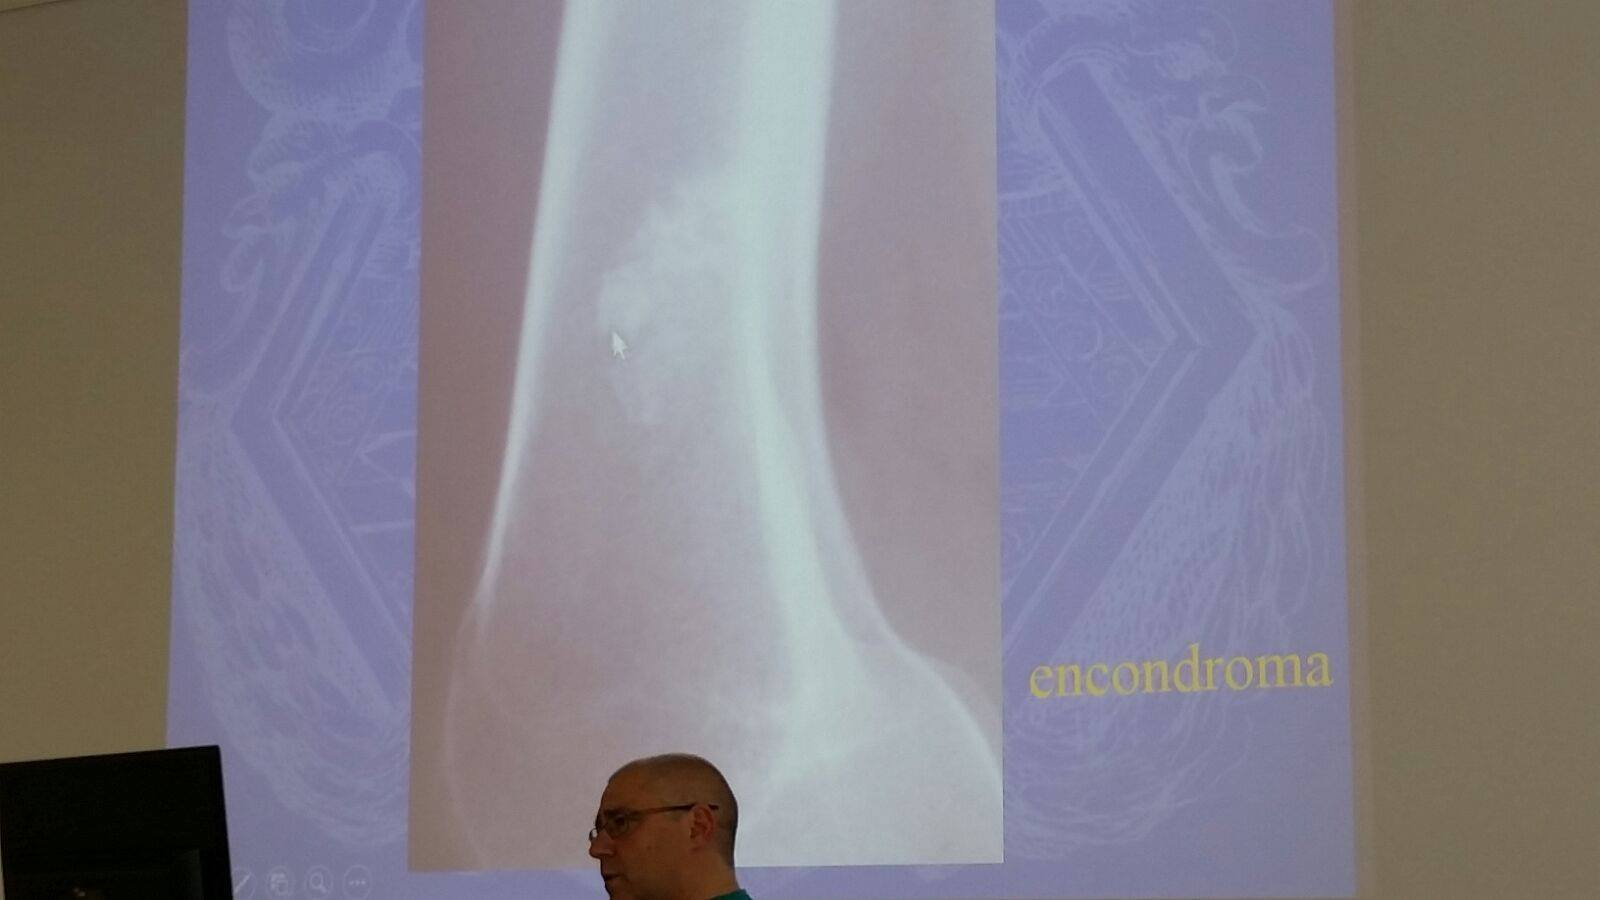
\includegraphics[width=3.41667in,height=2.49653in]{media/image1.jpeg}

La sintomatologia è dovuta ad un \textbf{aumento pressorio} all'interno
di questo canale inestensibile (da alcuni studi si è visto che si può
passare da 2,5 mmHg a più di \textbf{30 mmHg}).

Due posizioni (flessione palmare e dorsale) aumentano molto la pressione
all'interno del canale carpale, soprattutto in questo tipo di patologia,
e sono utilizzate come test specifici per fare diagnosi della patologia.

Cause

Le cause di aumento pressorio all'interno del tunnel carpale sono tutte
quelle condizioni che portano a:

\begin{itemize}
\item
  ESPANSIONE del contenuto del canale
\item
  RESTRINGIMENTO di ciò che sta attorno al tunnel carpale.
\end{itemize}

Tra le varie cause troviamo:

\begin{itemize}
\item
  ispessimento del legamento trasverso del carpo
\item
  processo infiammatorio tendineo e peritendineo dei tendini flessori
  (una delle cause più frequenti)
\item
  neoformazioni, lipomi, cisti all'interno del canale carpale
\item
  frammento osseo di frattura che schiaccia il nervo
\item
  callo osseo esuberante dopo una frattura di polso
\item
  osteofiti derivanti da malattie degenerative
\item
  deposizione sostanze patologiche (come in gotta, amiloidosi,
  insufficienza renale,\ldots{})
\item
  tumori intraneurali (neurinomi del nervo mediano)
\end{itemize}

\emph{Epidemiologia }

\begin{itemize}
\item
  E' più frequente nel sesso femminile, spesso in età perimenopausale
  (40-60 anni).
\item
  Il sesso maschile è meno coinvolto: riguarda perlopiù soggetti con
  attività lavorative che comportano prese di forza, movimenti ripetuti
  o uso di strumenti vibranti.
\item
  Nella maggior parte dei casi è colpito il lato dominante, ma ci può
  anche essere una bilateralità.
\item
  Può essere isolata o associata ad altre patologie della mano:
  \textbf{sindrome di De Quervain}, \textbf{dito a scatto},
  \textbf{rizartrosi}.
\end{itemize}

\emph{Eziopatogenesi }

\begin{itemize}
\item
  Idiopatica
\item
  Secondarie:
\end{itemize}

\begin{itemize}
\item
  Le condizioni già viste che causano aumento di pressione
\item
  Condizioni che aumentano la \emph{suscettibilità del nervo} (come il
  diabete o \emph{anomalie congenite} del nervo mediano stesso, ad
  esempio il nervo mediano bipartito, che aumentano la suscettibilità
  del nervo stesso).
\end{itemize}

\begin{itemize}
\item
  Forme acute come quelle post-traumatiche.
\item
  La causa più frequente che riduce lo spazio è la \emph{TENOSINOVITE
  DEI FLESSORI} che vanno a schiacciare il nervo mediano.
\item
  \emph{Può poi essere dovuta o a una condizione di
  \textbf{\emph{aumento del volume del contenuto del canale}} (ad
  esempio per \emph{cisti sinoviali} o \emph{infiammazione delle guaine
  tendinee}, ma anche per \emph{tumori} o per altre \emph{patologie
  espansive}) oppure una \textbf{\emph{riduzione delle dimensioni del
  tunnel stesso}}, che può essere dovuta o ad \emph{esiti di fratture
  del polso} guarite con un vizio di consolidazione, o anche ad una
  \emph{tenovaginite cronica ipertrofica}, la quale è nella maggior
  parte dei casi idiopatica e legata probabilmente anche ad alcuni
  \textbf{fattori ormonali} (in particolare il calo degli estrogeni) e
  ai \textbf{microtraumatismi} (come le attività lavorative con prese di
  forza o movimenti ripetitivi del polso), mentre più raramente la causa
  è \textbf{\emph{reumatologica}}.}
\end{itemize}

Ci sono patologie che favoriscono l'insorgenza del tunnel carpale :

\begin{itemize}
\item
  diabete
\item
  patologie tiroidee
\item
  iperaldosteronismo
\item
  Insufficienza renale cronica
\item
  gravidanza e allattamento (che, anche se non sono condizioni
  patologiche, sono comunque predisponenti all'insorgenza della
  sindrome. A fine gravidanza e allattamento la sintomatologia recede)
\end{itemize}

In queste patologie (diabete, patologie tiroidee, iperaldosteronismo),
l'esito dipende dal trattamento della patologia di base, perciò bisogna
sempre dire al paziente che il recupero potrebbe non essere completo se
il nervo è già rovinato dalla sottostante patologia.

\begin{itemize}
\item
  Bisogna prestare attenzione anche agli scoagulati.
\item
  Bisogna sempre aprire un gesso che dà fastidio, perché se troppo
  stretto potrebbe dare una compressione nervosa.
\item
  Lussazione delle ossa carpali possono dare compressione.
\item
  Trombosi dell'arteria (raro)
\end{itemize}

Ricapitolando, le cause più frequenti di compressione sono :

\begin{itemize}
\item
  ISPESSIMENTO LEGAMENTO TRASVERSO DEL CARPO
\item
  PROCESSO ESPANSIVO/INFIAMMATORIO DEI TENDINI FLESSORI CHE PASSANO
  ALL'INTERNO DEL TUNNEL CARPALE
\end{itemize}

\emph{Diagnosi}

Nella maggior parte dei casi si presenta una signora (perché appunto le
femmine sono maggiormente colpite rispetto ai maschi ), che di notte si
sveglia alla stessa ora perché si sente la mano pesante e addormentata
nella zona di innervazione del nervo mediano.

Quindi, dopo aver scrollato la mano per 1-2 minuti, questa sensazione
passa e la paziente si riaddormenta.

Durante il giorno questa sintomatologia ritorna soprattutto in movimenti
di \emph{presa statica} (quando si guida, si va in bici), con
\textbf{formicolii} simili alla sintomatologia notturna, spesso
associati a sensazione di \textbf{tumefazione}.

Ci può essere \textbf{dolore} fino alla radice delle dita o che risale
fino al gomito ed alla spalla (irradiazione prossimale).

Al mattino c'è una maggiore rigidità dell'articolazione.

D'inverno i sintomi si verificano molto più frequentemente che d'estate.

Negli stadi avanzati queste sensazioni di alterata sensibilità e di
dolore diventano costanti e si può arrivare all'\textbf{ipotrofia
dell'eminenza tenar} con difficoltà nello svolgimento di movimenti fini
delle dita (in passato le donne riferivano l'impossibilità di cucire).

Il dolore con il tempo tende a scomparire.

Di solito i sintomi sensitivi anticipano quelli motori (è raro che
avvenga il contrario).

Il decorso di solito non è particolarmente veloce, anche se in alcuni
casi (ad esempio negli anziani e nei diabetici, dove ci possono essere
altre neuropatie) l'insorgenza è acuta e si aggrava velocemente.

\emph{Obiettività }

Bisogna innanzitutto osservare la mano e ricercare:

\begin{itemize}
\item
  Eventuali deformità
\item
  Ipotrofia dell'eminenza tenar
\item
  Se il paziente riesce ad effettuare il movimento di opposizione
  (controllato dal ramo motorio del n. mediano)
\end{itemize}

Esistono dei test neurologici come:

\begin{itemize}
\item
  Test di discriminazione di due punti statici (di Weber)
\item
  Test di soglia
\item
  Valutare se ci sono deficit motori, osservando l'abduttore breve e
  l'opponente del pollice e il flessore breve delle dita.
\end{itemize}

Si fanno poi dei test provocativi :

\begin{itemize}
\item
  \emph{Test di Tinel}: percussione a livello del passaggio del nervo
  mediano nel canale carpale. È positivo se c'è una sensazione di scossa
  nella zona di innervazione del nervo mediano
\item
  \emph{Test di Phalen normale}: si chiede al paziente di mettere le
  mani dorso contro dorso, tenendo i gomiti a 90 gradi. E' positivo se
  entro 60 secondi compare formicolio anche intenso se il nervo mediano
  è compresso.
\end{itemize}

\begin{quote}
\emph{\emph{Nb: è bene tenere a mente che questi due test sono
sicuramente positivi nelle prime fasi, mentre in fase paralitica possono
anche risultare negativi.}}
\end{quote}

\begin{itemize}
\item
  \emph{Test di Phalen inverso}: c'è una flessione dorsale della mano e,
  anche in questo caso, è positivo se il paziente avverte formicolio
  entro 60 secondi nella zona di innervazione del nervo mediano
\item
  \emph{Test di Durkan}: si schiaccia il nervo in corrispondenza del
  tunnel carpale. Di solito è positivo se compaiono i sintomi dopo 30
  secondi dalla compressione.
\end{itemize}

\textbf{Diagnosi differenziale:}

\begin{itemize}
\item
  Una compressione C5-C6 del rachide, che presenta una sintomatologia
  simile.
\item
  Alcune patologie neurologiche possono dare sintomi simili, quindi
  bisogna fare attenti esami neurologici.
\item
  Considerare sempre il diabete, che può avere una neuropatia di base.
\end{itemize}

\emph{Esami strumentali}

L'\emph{elettromiografia} è un esame elettrofisiologico in cui si
applicano delle scosse prossimalmente al livello della compressione e si
registra la velocità di propagazione dell'impulso→ se è bassa vuol dire
che c'è la compressione del nervo.

Permette quindi di rilevare il \textbf{grado} di compressione del nervo
e quanto è grave questa compromissione. Rileva anche la
\textbf{localizzazione} della compressione del nervo: se la compressione
è prossimale (a livello del gomito) o se è distale, a livello del polso.

Questo è un aiuto importante dal punto di vista della scelta terapeutica
e nel post-operatorio una rivalutazione elettromiografica permette di
capire se l'intervento è riuscito.

L'\emph{ecografia} è un altro esame che si può fare. È un esame di
supporto, però molto meno usato rispetto all'elettromiografia. Usata in
caso di sospette lesioni ai tessuti molli.

L\emph{'Rx} è utile solo in esiti di patologie ossee.

\emph{Classificazione Clinica }

A seconda del grado di compressione del nervo si distinguono:

\begin{enumerate}
\def\labelenumi{\arabic{enumi}.}
\item
  Fase \textbf{algico-irritativa:} in cui il nervo è neuroaprassico. Ci
  possono essere dei fastidi. \emph{Fase caratterizzata da parestesie
  prevalentemente notturne in corrispondenza della superficie palmare
  delle prime 3 dita della mano e della metà del quarto dito, cioè in
  quella che è l'area di innervazione del nervo mediano.}
\item
  Fase \textbf{parestesico-dolorosa:} in cui il nervo è più compresso,
  con alcune degenerazioni. \emph{Ai sintomi della fase precedente si
  associano anche \emph{ipovalidità} ed \emph{ipotrofia dei muscoli
  dell'eminenza tenar} (opponente del pollice, abduttore breve del
  pollice e capo superficiale del flessore breve del pollice) \emph{e
  dei primi due lombricali}, con anche ipoestesia nel territorio di
  innervazione e difficoltà nel controllo della presa degli oggetti}
\item
  Fase \textbf{atrofico-paralitica:} è la fase finale, la più grave,
  caratterizzata anche da disturbi motori. \emph{\emph{Marcata atrofia
  dei muscoli dell'eminenza tenar associata ad ipoanestesia delle prime
  3 dita e della metà del quarto, con abolizione del movimento di
  opposizione del pollice.}}
\end{enumerate}

\includegraphics[width=3.93750in,height=3.09861in]{media/image2.jpeg}

Le fasi 1 e 2 sono reversibili con il trattamento.

Nella fase 3, anche se si va ad intervenire con un intervento
chirurgico, sarà molto difficile avere una restitutio ad integrum: ci
saranno dei miglioramenti dal punto di vista sintomatologico, ma non ci
sarà miglioramento dal punto di vista della forza e dell'atrofia del
muscolo.

\emph{Il recupero sarà tanto più veloce tanto più è stata breve la
compressione e sarà tanto più completo quanto meno grave è stata la
compressione.}

\emph{Trattamento}

\begin{itemize}
\item
  \textbf{Conservativo} (Stadi 1 e 2): nello stadio 1 si possono fare
  delle \emph{infiltrazioni di corticosteroidi} (massimo due all'anno)
  all'interno del canale carpale, attorno al nervo e ai tendini che
  molto spesso sono infiammati.
\end{itemize}

\begin{quote}
Si possono fare anche \emph{terapie fisiche}.

Ma soprattutto ha un effetto positivo il trattamento con \emph{tutori}
(solo di notte o giorno e notte) che evitano posizioni di iperestensione
e di iperflessione che aumenterebbero la pressione nel canale. Essi
immobilizzano il polso in \emph{posizione neutra} (2-9º in flessione
dorsale, 2-6º di deviazione ulnare), in cui il nervo è stressato al
minimo.
\end{quote}

\begin{itemize}
\item
  Nello stadio 2 e 3 (o qualora il trattamento conservativo non abbia
  avuto effetto) si può arrivare al \textbf{trattamento chirurgico}:
  consiste nell'apertura del tunnel carpale attraverso la \emph{sezione
  del legamento trasverso del carpo} senza danneggiare il nervo mediano
  che sta sotto. E' effettuato in anestesia locale, quindi in regime
  ambulatoriale.
\end{itemize}

\begin{quote}
Si può fare:
\end{quote}

\begin{itemize}
\item
  \emph{a cielo aperto} attraverso l'incisione classica: incisione del
  palmo della mano lungo l'asse del quarto dito, si scolla cute e
  sottocute e si seziona longitudinalmente il legamento trasverso del
  carpo. Una volta sezionato, sotto si trova il nervo e attorno i
  tendini: se il nervo è troppo compresso si può fare una
  \textbf{neurolisi}, cioè si libera il nervo dalle aderenze e a volte
  si toglie anche la sinovia che infiamma il tendine.
\end{itemize}

\begin{quote}
{[}Per differenziare \emph{nervi e tendini, basta piegare passivamente
le dita: il nervo resta fisso mentre} i tendini scorrono{]}.

Si possono anche fare delle mini incisioni a livello del polso e del
palmo della mano, si passa sotto con una sonda e si seziona per via
sottocutanea.
\end{quote}

\begin{itemize}
\item
  per via endoscopica che offre minori tempi di recupero ma con un
  maggior rischio di complicanze intraoperatorie.
\end{itemize}

\emph{In ogni caso, il trattamento chirurgico garantisce un netto
miglioramento del dolore ed un buon recupero sensitivo e motorio, purché
si sia andati ad agire tempestivamente (infatti più a lungo il nervo
rimane compresso e tanto minore sarà il recupero, fino ad essere del
tutto assente).}

\emph{Post-operatorio}

In genere si esegue un \textbf{bendaggio} o si utilizza un
\textbf{tutore}.

Si dice al paziente di muovere le dita e di tenere in alto la mano
affinché non si provochino ematomi.

Dopo 2 settimane si tolgono i punti ed inizia la cura della cicatrice,
che può dar fastidio per 1-2 mesi. Si consigliano \emph{massaggi} (2-3
volte al giorno per una ventina di giorni) per far passare il fastidio
legato alla cicatrice.

Si possono associare anche \emph{ultrasuoni}.

È necessario avvisare il paziente che non ritornerà subito completamente
alla manualità precedente perché i tempi di pieno recupero sono di circa
1-2 mesi.

\emph{Complicanze}

Può sembrare un intervento banale ma il rischio più grave è il
\textbf{taglio della branca motoria del nervo mediano.} Essa normalmente
si sfiocca oltre il legamento trasverso mediano.

Ci possono però essere delle varianti anatomiche in cui si sfiocca al di
sotto o dentro il legamento trasverso: per questo nel sezionare è meglio
portarsi verso il lato ulnare piuttosto che direttamente sopra il nervo.

Ovviamente non bisogna stare troppo sul lato ulnare perché si rischia di
lesionare il nervo ulnare.

Altra complicazione può essere la recidiva per cicatrizzazione ed
inspessimento del legamento trasverso del carpo.

\includegraphics[width=5.68819in,height=2.34375in]{media/image3.jpeg}

\emph{Altri siti di compressione dei nervi nell'arto superiore }

\emph{Nervo Ulnare}

Può avere 2 siti di compressione:

\begin{itemize}
\item
  a livello della \textbf{doccia epitrocleolecranica} del gomito.
\end{itemize}

SINTOMI: intorpidimento lungo la zona di innervazione sensitiva del
nervo ulnare e nei casi gravi ipotrofia dell'eminenza tenar.

\begin{itemize}
\item
  \textbf{Sindrome del canale di Guyon} se è compresso a livello del
  polso.
\end{itemize}

\emph{Nervo Mediano}

\begin{itemize}
\item
  A livello del \textbf{canale carpale}
\item
  \textbf{Sindrome del nervo INTEROSSEO ANTERIORE:} quando compresso
  nella sua branca motoria a livello del gomito.
\end{itemize}

\begin{quote}
SINTOMI: prevalentemente motori, a livello dei muscoli dell'avambraccio.
\end{quote}

\emph{Nervo Radiale}

\begin{itemize}
\item
  Può essere lesionato e stirato nelle fratture del terzo distale
  dell'omero
\item
  \textbf{Compressione del} \textbf{nervo INTEROSSEO POSTERIORE:}
  compressione della sua componente motoria, che innerva i muscoli
  estensori delle dita.
\item
  Compressioni più alte a livello sottoclavicolare (legate per esempio
  ad una sindrome dello sbocco toracico).
\end{itemize}

\emph{Patologie compressive nell'arto inferiore}

\begin{itemize}
\item
  \textbf{Sindrome del tunnel tarsale:} è il corrispettivo, a livello
  del piede, della sindrome del tunnel carpale. Consiste nella
  compressione del \emph{nervo tibiale posteriore} a livello della
  doccia retromalleolare mediale.
\end{itemize}

SINTOMI: formicolii a livello della pianta del piede.

\begin{itemize}
\item
  \textbf{Compressione del nervo sciatico popliteo} \textbf{esterno} a
  livello della testa del perone (particolarmente vero nelle forme acute
  delle fratture del piatto tibiale oppure nelle forme acute nel caso di
  pazienti allettati da molto tempo e che tendono ad avere la gamba
  extra ruotata, per cui il nervo può essere schiacciato, ma ci sono
  anche forme idiopatiche).
\item
  \textbf{Sindrome del piriforme:} è una sindrome per esclusione (nello
  sportivo soprattutto), da compressione del nervo sciatico dal bordo
  inferiore del muscolo piriforme. Il nervo sciatico può essere
  lesionato o compresso quando si ha una lussazione dell'anca.
\item
  Il \textbf{nervo femorale} a volte può essere stirato quando si fa un
  accesso laterale all'anca: uno stiramento da parte dei divaricatori
  può essere presente nella artrosi concentriche dell'anca.
\end{itemize}

\end{document}



\section{Fratture del Collo del Femore}

\subsection{Definizione}

Il \textbf{femore} è il più grande osso lungo del nostro organismo, e
dal punto di vista anatomico può essere generalmente suddiviso in una
\emph{parte centrale}, il \emph{corpo}, detto più propriamente
\textbf{\emph{diafisi}}, e in due estremità, dette
\textbf{\emph{epifisi}}, di cui la prossimale si articola con l'osso
dell'anca formando l'articolazione coxo-femorale, mentre quella distale
si articola con la rotula e la tibia, formando l'articolazione del
ginocchio; le diafisi e le epifisi sono unite tra loro da delle regioni
che prendono il nome di \textbf{\emph{metafisi}}, e che durante
l'adolescenza corrispondono alle aree occupate dalla cartilagine di
accrescimento, che fino alla chiusura delle metafisi consente
l'allungamento dell'osso.
\begin{figure}[!ht]
\centering
	\includegraphics[width=0.5\textwidth]{007/image1.jpeg}
\end{figure}
Quando si parla di \textbf{fratture del collo del femore} si intendono
quindi le fratture che \emph{riguardano l'epifisi prossimale}, la quale
ha una struttura anatomica peculiare e risulta costituita da una
\textbf{testa}, sostenuta da un \textbf{collo}, alla due base di trovano
due prominenze ossee, note come \textbf{grande} \textbf{trocantere} e
\textbf{piccolo} \textbf{trocantere} del femore.

Bisogna inoltre ricordare che per \textbf{\emph{frattura}} si intende
una qualsiasi lesione che causa una \emph{soluzione di continuità
all'interno dell'osso stesso}, determinata da una forza la cui intensità
supera la resistenza elastica dell'osso stesso: in questa definizione
rientrano quindi due variabili principali, che sono appunto
l'\emph{intensità della forza} e la \emph{resistenza dell'osso}, da cui
deriva anche che esistono due forme principali di fratture, le
\textbf{fratture propriamente dette}, in cui la resistenza dell'osso è
normale, ma l'intensità della forza è sufficientemente elevata da
vincerla, e le \textbf{fratture patologiche}, in cui la resistenza ossea
è diminuita, ad esempio a causa di cisti ossee, metastasi tumorali,
osteopetrosi o osteoporosi (in realtà l'osteoporosi non rientra nelle
fratture patologiche propriamente dette, ma è comunque considerata una
condizione borderline), e in tutti questi casi la forza applicata non
avrebbe intensità tale da determinare una frattura in un osso sano, ma
riesce a causarla a causa della marcata compromissione della resistenza
ossea.

Quando poi si parla di \textbf{\emph{osso}}, è importante precisare in
base a quale punto di vista lo si sta valutando, perché per osso si può
intendere o come \emph{organo} (il femore, l'omero, ecc) oppure come
\emph{tessuto}, in questo caso formato da osteoni, componente inorganica
ed organica, deputato a svolgere un'importante funzione meccanica, e
infatti al suo interno la struttura è disposta in \textbf{lamelle
ossee}, le quali non sono collocate a caso, ma sono disposte secondo le
linee di forza che agiscono su quel determinato segmento osseo, e in
particolare a livello del collo del femore abbiamo due fasci principali,
un \emph{fascio principale che contrasta le forze tensive}, teso tra la
testa del femore e la base del grande trocantere, ed un \emph{fascio
principale che contrasta le forze comprensive}, cioè il carico, che va
dalla testa del femore sino alla base del collo, appena sopra al piccolo
trocantere. Questi due fasci si incrociano quindi all'interno del collo,
determinando un'area che in sezione appare triangolare e prende appunto
il nome di \textbf{triangolo di Ward}, ben osservabile nel giovane
adulto, ma che con l'invecchiamento e l'osteoporosi tende ad
ingrandirsi, determinando purtroppo una riduzione della resistenza in
quest'area.
\begin{figure}[!ht]
\centering
	\includegraphics[width=0.5\textwidth]{007/image2.jpeg}
\end{figure}
\subsection{Epidemiologia delle Fratture del Collo del Femore}

Dal punto di vista epidemiologico, si tratta di fratture che sono
piuttosto frequenti nell'\emph{età avanzata}, mentre sono più rare nei
giovani, e purtroppo nell'anziano la frattura del collo del femore è una
condizione che tende ad aggravare le altre patologie concomitanti in
maniera anche molto significativa. Sempre dal punto di vista
epidemiologico, tuttavia, bisogna anche precisare che nei soggetti
giovani, la frattura mediale del collo femorale è tipicamente correlata
con traumi ad alta energia, quali possono essere incidenti
motociclistici, il pattinaggio o gli sci, e sono condizioni altamente
problematiche, poiché le fratture mediali determinano spesso una necrosi
ischemica della testa del femore.

\subsection{Osteoporosi}


Si intende per osteoporosi la riduzione della massa ossea nell'ambito
del nostro apparato scheletrico. Bisogna ricordare però che l'osso è un
organo biologico costituito da cellule, a funzione meccanica, ed è per
questo che possono essere inserite viti al suo interno, perché possiede
una resistenza meccanica. Nel corso della vita, la fisiologia del
tessuto osseo fa sì che questo si modifichi: la parte tubulare dell'osso
si allarga in diametro ma aumenta il canale midollare, determinando una
riduzione della sua resistenza in quanto si avrà uno squilibrio tra
posizione e riassorbimento con prevalenza del riassorbimento osseo (ecco
perché da giovani si hanno mani più piccole: con l'invecchiamento le
falangi si allargano divenendo più deboli dal punto di vista meccanico).
Queste modifiche però, non vanno considerate come patologiche, ma come
fisiologia nell'ambito dell'invecchiamento: questo vale per tutti gli
organi (potrebbe entrare nell'ambito della patologia qualora trovassimo
la cura). L'osteoporosi, quindi, non è considerabile una vera e propria
patologia, anche se ovviamente le considerazioni variano in base al
contesto in cui si colloca, ad esempio è ovvio che l'osteoporosi in una
pz di 50 anno alla quale sono stati tolti utero ed ovaie per fibromi a
25 anno, non può essere considerata fisiologica.

\subsection{Classificazione delle Fratture del Collo del Femore}


Esistono diverse classificazioni delle fratture del collo femorale, ma
la più importante dal punto di vista didattico è quella \emph{su base
anatomica}, che le suddivide, rispetto alla linea intertrocanterica, in:

\begin{itemize}
\item
  \textbf{\emph{Fratture Mediali}}, che sono quelle che avvengono
  medialmente all'inserzione della capsula articolare, verso la linea
  mediana;
\item
  \textbf{\emph{Fratture Laterali}} e \textbf{\emph{Pertrocanteriche}},
  che si hanno al di fuori della capsula e sulla linea
  intertrocanterica.
\end{itemize}

Questa classificazione è importantissima dal punto di vista prognostico,
perché \emph{le fratture mediali possono determinare interruzione della
vascolarizzazione a livello della testa del femore}, in quanto si ha una
lesione a livello capsulare, mentre le pertrocanteriche e le laterali
presentano una prognosi migliore perché non determinano un'interruzione
della vascolarizzazione di questo distretto. La capsula articolare,
infatti, può essere vista come un tubo o una guaina che stabilizza
l'articolazione coxo-femorale e possiede, oltre all'inserzione a livello
del bordo circonferenziale del cotile, anche un'inserzione a livello
della linea intertrocanterica: questa disposizione è molto importante
perché si riflette anche sulla \textbf{vascolarizzazione}, infatti la
vascolarizzazione del collo femorale deriva in gran parte dalle
\emph{arterie circonflesse anteriori} e dall'\emph{arteria circonflessa
posteriore}, mentre la vascolarizzazione della testa è a carico di rami
che si dipartono sempre dall'arteria circonflessa, la quale decorre nel
punto in cui la capsula articolare si inserisce a livello della linea
intertrocanterica, e anche dell'\emph{arteria del legamento rotondo},
che deriva dall'arteria otturatoria, la quale nel 60-70\% dei casi con
la maggiore età va incontro ad obliterazione. Da questa peculiare
vascolarizzazione ne deriva che una frattura che interrompe la
vascolarizzazione a livello della teste determina in genere ischemia con
possibile necrosi, ma se l'individuo con questo tipo di frattura ha la
fortuna di possedere l'arteria del legamento rotondo pervia, la frattura
può anche non andare incontro a necrosi, ecco perché non tutte le
fratture mediali del collo femorale esitano nella necrosi ischemica
della testa del femore.
\begin{figure}[!ht]
\centering
	\includegraphics[width=0.8\textwidth]{007/image4.jpeg}
\end{figure}

\subsection{Meccanismo Traumatico delle Fratture del Collo Femorale}


In genere, le cause di questo tipo di fratture sono condizioni
relativamente banali, come \emph{cadute in casa}, o in condizioni o
luoghi pericolosi, ma va tenuto a mente che \textbf{spesso il paziente
cade perché si frattura, e non il contrario}: in seguito ad un
inciampamento, ad esempio, il femore subisce una \emph{torsione}, con
\emph{improvviso aumento del carico che determina la frattura}, che a
sua volta causa un'\emph{impotenza funzionale improvvisa ed il paziente
cade}. È inoltre importante capire se il paziente è caduto perché si è
rotto il femore o se ha avuto un TIA, e per discriminare tra le due
condizioni è bene fare alcune valutazioni, ad esempio se è presente
anche una frattura del polso si deve pensare ad una reazione di difesa,
per cui il paziente era cosciente e ha cercato di attutire la caduta,
mentre se vi è una frattura a livello del viso, la rottura del naso o un
ematoma del volto si deve pensare ad un TIA, perché non c'è stata
probabilmente alcuna risposta di difesa da parte del paziente.

\subsection{Fratture Mediali}


Le fratture mediali del femore possono a loro volta essere sotto
classificate in:

\begin{itemize}
\item
  \textbf{\emph{Fratture Mediali Sottocapitate}}, che interessano la
  porzione più alta del collo femorale, appena sotto alla testa;
\item
  \textbf{\emph{Fratture Mediali Mediocervicali}}, che interessano la
  porzione intermedia del collo;
\item
  \textbf{\emph{Fratture Mediali Basocervicali}}, che sono poste alla
  base del collo, e sono delle fratture borderline, nel senso che non è
  sempre facile discriminarle dalle fratture pertrocanteriche.
\end{itemize}
\begin{figure}[!ht]
\centering
	\includegraphics[width=0.5\textwidth]{007/image5.jpeg}
\end{figure}
Esistono anche altre sottoclassificazioni, come la
\textbf{\emph{classificazione di Garden}} {[}vedi Internet{]}, che
distingue le fratture in base al \emph{movimento traumatico},
suddividendole in \textbf{fratture per abduzione}, in cui l'arto
inferiore viene abdotto in modo forzato, e in \textbf{fratture per
adduzione}, in cui il paziente cade con la coscia sotto al bacino e si
ha una adduzione forzata..
\begin{figure}[!ht]
\centering
	\includegraphics[width=0.5\textwidth]{007/image6.jpeg}
\end{figure}
\paragraph{Quadro Clinico}

Per quanto riguarda il quadro clinico, non esistono differenze molto
significative tra fratture mediali e laterali, sebbene vi possano essere
alcune sfumature sintomatologiche; il \textbf{dolore}, dovuto
all'intensa stimolazione delle fibre nervose del periostio, è molto
intenso e localizzato in \emph{sede inguinale}, ma può avere una
localizzazione più ampia se la frattura è esposta e si ha anche
lacerazione delle parti molli circostanti. Peculiare è poi
l'\textbf{extrarotazione dell'arto}, atteggiamento tipico della fratture
dell'epifisi femorale prossimale, sia mediale che laterale, con
\textbf{accorciamento di tutto l'arto} ed \textbf{impotenza funzionale}
nella flessione dell'anca a ginocchio esteso, in quanto qualsiasi
frattura del collo del femore, non permette la manovra di elevazione di
tutto l'arto senza flettere il ginocchio. Nonostante ciò, è bene tenere
a mente che alcuni pazienti con fratture di tipo Garden I, cioè
ingranate e ben composte, riescono comunque a camminare, sono
relativamente stabili e riferiscono solo un dolore in sede inguinale, e
in questi casi la diagnosi può richiedere una TC, in quanto all'Rx solo
un occhio esperto è in grado di vedere che le lamelle ossee hanno un
orientamento diverso tra loro.
\begin{figure}[!ht]
\centering
	\includegraphics[width=0.5\textwidth]{007/image9.jpeg}
\end{figure}


\paragraph{Quadro Radiografico}

All'Rx, è necessario fare sempre due proiezioni ortogonali, una
\emph{antero-posteriore} e l'altra \emph{latero-laterale}, quest'ultima
in realtà chiamata \textbf{proiezione} \textbf{inguinale}, poiché
effettuata tramite proiezioni ginecologica dell'altro arto. Segni
radiologici valutabili confrontando l'arto patologico con quello
controlaterale sano sono i seguenti:

\begin{itemize}
\item
  In proiezione inguinale si vede bene l'\emph{extrarotazione dell'arto
  col grande trocantere spostato verso il basso};
\item
  Si può osservare un'\emph{interruzione delle lamelle ossee}, che
  permette di valutare anche le fratture composte, le quali hanno
  comunque un rischio non indifferente di andare incontro a
  scomposizione;
\item
  \emph{L'angolo tra collo e diafisi, in genere di 125\textsuperscript{o}, è aumentato},
  soprattutto nel confronto con l'arto controlaterale;
\item
  In proiezione inguinale, \emph{l'asse del collo non viene mantenuto};
\item
  La \textbf{\emph{linea di Shenton}}, cioè la linea che congiunge la
  parte inferiore della branca ileo pubica alla parte mediale del collo
  del femore, \emph{è interrotta per la presenza di una deviazione in
  varo del collo}.
\end{itemize}
\begin{figure}[!ht]
\centering
	\includegraphics[width=0.5\textwidth]{007/image10.png}
\end{figure}
\subsection{Fratture Laterali del Collo Femorale}


Anche in questo caso, possono essere sotto classificate in diversi tipi:

\begin{itemize}
\item
  \textbf{\emph{Fratture Laterali Basicervicali}}, cioè fratture
  borderline che si possono riscontrare anche nelle mediali;
\item
  \textbf{\emph{Fratture Laterali Transtrocanteriche}};
\item
  \textbf{\emph{Fratture Laterali Pertrocanteriche}}, che sono le
  comuni, tanto da essere considerate le fratture laterali per
  antonomasia. A volte possono essere fratture comminute, in cui si
  stacca solo il piccolo trocantere perché tirato dal muscolo ileopsoas.
\item
  \textbf{\emph{Fratture Laterali Isolate dei Trocanteri}}, che non sono
  fratture articolari e sono tipiche dei ciclisti; nei casi più
  complessi si può osservare la testa del femore che sfonda la lamina
  quadrilatera del bacino, creando delle lesioni gravissime
\item
  \textbf{\emph{Fratture Laterali Sottotrocanteriche}}.
\end{itemize}

Dal punto di vista clinico la sintomatologia è sovrapponibile a quella
riscontrata nelle fratture mediali, con dolore in sede inguinale,
impotenza funzionale nella flessione dell'arto a ginocchio esteso,
accorciamento dell'arto, extrarotazione. Tipica è poi la presenza di
\emph{ecchimosi} e di \emph{ematomi}: le ecchimosi si presentano come
soffusioni emorragiche a livello di cute e sottocute, mentre gli ematomi
sono raccolte di sangue in una cavità non preformata (altrimenti sarebbe
un emartro o un'altra condizione specifica), ma all'interno di un
muscolo o del sottocute, e dal punto di vista semiologico l'ematoma è
facile da riconoscere perché si presenta come un ``bozzo'' apprezzabile
alla palpazione, che si muove rispetto ai tessuti limitrofi. Se una
frattura mediale non è molto scomposta e non rompe la capsula, il sangue
che esce dall'osso fratturato rimane dentro la capsula e non si creano
né ecchimosi né ematoma; se invece la frattura è pertrocanterica, cioè
posta al di fuori della capsula, lo stravaso ematico che segue la
frattura può andare a colonizzare il sottocute, determinando la
formazione appunto di ecchimosi ed ematomi.

\subsection{Terapia e Complicanze delle Fratture del Collo Femorale}


Il trattamento delle fratture del collo del femore è ovviamente
condizionato dalle eventuali comorbilità del paziente, ad esempio in un
diabetico in trattamento adeguato con poche unità di insulina o con
ipoglicemizzanti orali, a seguito della frattura si può avere uno
scompenso metabolico che mette fuori controllo il diabete, poiché si
sviluppa una sindrome da adattamento con attivazione dell'asse
ipotalamo, ipofisi-surrene ed con un aumento dei livelli circolanti di
cortisolo, che causa appunto insulino-resistenza e fa sì che il diabete
non sia più ben controllabile, oppure in caso di un paziente
cardiopatico, uno stimolo intensamente doloroso come la frattura può
determinare lo sviluppo di uno scompenso cardiaco, per cui bisogna
sempre tenere conto del contesto in cui si va ad agire.

Dopo la diagnosi, quindi, la prima cosa che si dovrebbe fare è la
\textbf{trazione a zampale}, cioè una trazione modesta, di non più di 2
Kg, per cercare di dominare l'atteggiamento extra-rotatorio determinato
dalla frattura del collo del femore, in particolare dalla rottura del
segmento intertrocanterico, e quindi cercare di ridurre il dolore, così
da dominare anche la contrattura muscolare e l'accorciamento.

Il trattamento delle fratture del collo femorale, inoltre, è un
\emph{approccio prettamente chirugico}, che in molti ospedali viene
eseguito in urgenza (entro 3 giorni) o al più in urgenza differita
(entro 7 giorni). In generale, proprio a causa delle comorbilità, prima
si opera, meglio i pazienti stanno (a Parma si cerca di operare entro le
prime 12-24 ore se possibile, così da evitare la sindrome da
allettamento o lo sviluppo di piaghe da decubito, infezioni delle vie
urinarie e TEP). Lo scopo del trattamento è quindi quello di
\emph{ridurre il più possibile il periodo di allettamento},
\emph{consentire una mobilizzazione precoce} e \emph{ridurre di
conseguenza le complicanze generali} (N.B.: La frattura del collo del
femore, in soggetti anziani, è una condizione molto grave, che provoca
complicanze potenzialmente letali, per cui, anche se l'intervento non è
scevro da rischio, è comunque bene tentarlo per dare al paziente un
chance di sopravvivere). È ovvio però che prima di procedere
all'intervento il paziente deve essere stabilizzato, in particolare
bisogna cercare di correggere il più possibile la glicemia e le
ipopotassiemie, così da rendere l'intervento il meno rischioso
possibile.

L'intervento chirurgico avviene in due passaggi:

\begin{enumerate}
\def\labelenumi{\arabic{enumi}.}
\item
  \textbf{Riduzione della Frattura}, in cui si rimettono a posto i
  frammenti , affrontando il problema dell'extrarotazione, per cui si
  devono esercitare delle forze uguali e contrarie a quelle della
  scomposizione, vale a dire trazione ed intrarotazione;
\item
  \textbf{Osteosintesi/Fissazione}, che può essere interna con placche,
  viti o chiodi, oppure esterna, che consiste nella fissazione senza
  ferite chirurgiche, applicando delle fiches transcutanee nel collo del
  femore, a livello della diafisi, il tutto collegato ad un fissatore
  esterno (in genere si preferisce ricorrere alla fissazione esterna
  quando la ferita è esposta, cioè quando non è possibile agire
  stabilizzandola internamente.
\end{enumerate}

\subsubsection{Trattamento delle Fratture Mediali}


Per le fratture mediali esistono \emph{3 opzioni di trattamento} a
seconda del tipo di lesione e della capacità funzionale del paziente:
\begin{figure}[!ht]
\centering
	\includegraphics[width=0.5\textwidth]{007/image13.jpeg}
\end{figure}
\begin{figure}[!ht]
\centering
	\includegraphics[width=0.2\textwidth]{007/image15.jpeg}
\end{figure}
\begin{itemize}
\item
  Per le \textbf{fratture mediali meno scomposte}, quindi con
  \emph{minor rischio di necrosi}, si conserva la testa e si fissa la
  frattura mediante osteosintesi con viti e placche, e questa procedura
  viene in genere effettuata tramite applicazione di due viti di
  titanio, parallele su di un piano e divergenti sull'altro, così da
  evitare la rotazione (in genere bastano due viti, perché si deve
  cercare di ridurre al minimo il rapporto tra osso e quantità di
  metallo, così da non svuotare la testa). In alternativa, per le
  \textbf{fratture basicervicali}, vengono usate viti e placche, con una
  vite più grossa ed una più piccola per evitare la rotazione. In questo
  caso la sintesi viene effettuata se il malato possiede capacità
  funzionale elevata ed ha la possibilità di stare un paio di mesi con
  le stampelle, per poi effettuare una protesi in un secondo momento se
  non migliora.
\item
  In caso di \textbf{frattura mediale in paziente con una capacità
  funzionale discreta} si applica un'\emph{endoprotesi}, cioè si
  sostituisce la testa, mettendola in rapporto col cotile originario. Si
  tratta quindi di una protesi parziale, ed è un intervento tipico di
  chi possiede appunto una capacità funzionale discreta ma non
  eccezionale, perché alla lunga si può sviluppare una
  \emph{cotiloidite}, cioè l'osso a livello del cotile si usura e fa
  male.
\item
  In caso di \textbf{frattura molto scomposta e ad elevato rischio di
  necrosi} \textbf{in una persona ad elevata capacità funzionale} si fa
  un'\emph{artroprotesi}, che consiste nella sostituzione della testa e
  del cotile, con lo stesso procedimento seguito per la coxatrosi: prima
  si incide la cute ed il sottocute, arrivando alla fascia lata che
  viene incisa, poi si scollano i muscoli glutei dal grande trocantere e
  si evidenzia, con l'uso di leve apposite, la capsula articolare in
  extrarotazione, la quale viene incisa a croce e tagliata attorno al
  cotile. A questo punto la testa del femore viene lussata e rimossa con
  appositi strumenti; il collo viene tagliato via con un seghetto e
  rifinito con seghe pneumatiche, poi si elimina il cotile originario
  tramite delle frese circolari e lo si sostituisce col cotile
  protesico, mentre a livello dello stelo femorale viene inserita
  l'endoprotesi. Infine, in caso di endoprotesi si mette la testa e si
  fa la riduzione senza componente acetabolare, mentre in caso di
  endoprotesi totale si fa la manovra al contrario. L'intervento si
  conclude con la sutura dei muscoli, della fascia lata e della cute.
\end{itemize}

\subsubsection{Trattamento delle Fratture Laterali}


Le fratture laterali hanno un braccio di leva molto diverso rispetto a
quelle mediali e di solito il trattamento viene effettuato tramite
\emph{viti e placche}, di cui esistono diversi modelli; il trattamento
chirurgico in questo caso prevede un'incisione più spostata verso il
ginocchio, più bassa rispetto al trocantere, e le placche vengono poi
inserite con angoli di inclinazione diversi a seconda della
conformazione dell'anca, mettendo un filo guida con trapani ad alta
velocità e si fa l'alloggio per il vettore grande, e lo si inserisce.
Tutti questi passaggi sono effettuati sotto al controllo di un
amplificatore di brillanza, uno strumento che presenta una visione
invertita rispetto alla radiologia tradizionale (cioè l'osso appare nero
invece che bianco), e nelle fratture pertrocanteriche è importante
mettere la vite nel quadrante inferiore, così da evitare che essa esca
dalla testa come conseguenza di un processo osteoporotico.
\begin{figure}[!ht]
\centering
	\includegraphics[width=0.5\textwidth]{007/image16.jpeg}
\end{figure}
\subsubsection{Trattamento Post-Operatorio}

Dopo il trattamento chirurgico, si deve procedere ad una
\emph{rieducazione funzionale non appena la ferita guarisce}, anche se
in realtà, se la comorbilità è bassa ed il montaggio buono, il paziente
con endoprotesi o con un chiodo gamma può essere messo un piedi subito.
La rieducazione funzionale è solo una parte della fisioterapia, e si
intende con questa definizione anche la rieducazione alla funzione della
deambulazione. È tuttavia ovvio che pazienti con fratture che non danno
garanzie di stabilità devono rimanere allettati per un certo periodo di
tempo, ma \emph{la fisioterapia è una componente importantissima che
deve essere iniziata il prima possibile}.

\subsubsection{Complicanze delle Fratture del Collo del Femore}

Le complicanze delle fratture del collo femorale, così come nelle
fratture generali, possono essere generalmente suddivise in
\textbf{complicanze generali} e \textbf{complicanze locali}:

\begin{itemize}
\item
  \textbf{\emph{Complicanze Generali}}: Si caratterizzano per un
  \emph{decadimento delle condizioni generali}, soprattutto in ambito
  geriatrico, perché il paziente diventa completamente dipendente dagli
  altri, ed anche l'aspetto psicologico grava significativamente sul
  paziente, con possibile insorgenza di depressione senile e conseguente
  scarsa motivazione alla fisioterapia.
\item
  \textbf{\emph{Complicanze Locali}}: Sono più frequenti nelle fratture
  mediali, e sono rappresentate essenzialmente dalla \emph{necrosi
  ischemica della testa del femore}, tipicamente in presenza di fratture
  molto scomposte, in cui è l'arteria del legamento rotondo è
  obliterata. Spesso si tenta comunque una sintesi, ma la necrosi può
  comparire dopo l'intervento, in un lasso di tempo che arriva anche a
  12 mesi, per cui è un'eventualità che va sempre tenuta in
  considerazione. Altra complicanza locale tipica delle fratture mediali
  è lo sviluppo di una \emph{pseudoartrosi}, condizione in cui alla
  testa del femore arriva una quantità ridotta di sangue, abbastanza per
  non dare necrosi, ma non sufficiente a garantirne la guarigione.
\end{itemize}


\section{Ginocchio (Pogliacomi)}

L'articolazione del ginocchio è un'articolazione che, dal punto di vista anatomico e biomeccanico, può essere considerata una doppia articolazione condiloidea fra i due condili del femore e i due piatti tibiali, a cui si associa poi l'articolazione trocleare fra la troclea
femorale e la rotula.
L'articolazione del ginocchio dal punto di vista osseo non è particolarmente stabile, ossia la convessità dei condili femorali non corrisponde precisamente con la concavità dei due piatti tibiali.
(Al contrario a livello dell'anca la congruenza articolare è particolarmente importante, la testa del femore forma una sorta di vuoto con l`acetabolo.)

Per dare stabilità a questo tipo di articolazione subentrano degli elementi stabilizzatori passivi e degli elementi stabilizzatori attivi. Attivi sono i gruppi muscolari la cui contrazione rinforza l'articolazione, tra questi vanno ricordati:

\begin{itemize}
\item
  i tendini del semimembranoso e i tendini della zampa d'oca medialmente
\item
  il sistema quadricipite-rotula-tendine rotuleo anteriormente,
\item
  il tendine del bicipite femorale in posizione laterale
\item
  i gastrocnemi in posizione posteriore.
\end{itemize}

Mentre i passivi sono la capsula e i legamenti. La capsula è essenzialmente un manicotto fibroso che unisce il femore alla tibia, rinforzata da diversi legamenti, cioè fasci di tessuto fibro-collageno denso, simili ai tendini, la cui posizione e disposizione corrisponde alle linee di tensione che entrano in funzione durante i movimenti articolari del ginocchio, ed analoga struttura hanno anche i legamenti crociati. In generale, il ginocchio è un'articolazione complessa, anche se il suo movimento avviene praticamente solo sul piano sagittale, in un meccanismo di flesso-estensione che va da 180\textsuperscript{o} a 30\textsuperscript{o}, e in questo movimento la superficie articolare della tibia ruota su quella del femore, ma il centro di tale rotazione non è fisso, ma tende a spostarsi in dietro col progredire della flessione. Quando il ginocchio è completamente esteso, ogni movimento che non sia di flessione è impossibile, mentre quando il ginocchio è flesso, sono concessi dei movimenti di rotazione della tibia rispetto al femore: nella rotazione interna, i due legamenti crociati si avvolgono tra loro e così la limitano; nella rotazione esterna, invece, si svolgono e la limitazione è allora principalmente affidata alla capsula mediale e al punto d'angolo postero-interno.
\\\\
È importante tenere a mente che, in condizioni normali, le strutture di sostegno dell'articolazione del ginocchio agiscono in modo sinergico tra loro, e la sezione di un solo legamento non produce alcuna instabilità del ginocchio, con l'eccezione del legamento crociato posteriore, la cui sezione determina immediata instabilità articolare, in quanto rappresenta il vero asse portante di questa articolazione. Il legamento crociato posteriore è un legamento robusto, si rompe solo con forze molto intense, e quindi la sua interruzione crea instabilità del ginocchio con sublussazione posteriore della tibia, ma fortunatamente è un legamento extra-articolare e le sue lesioni tendono a cicatrizzare piuttosto bene. Il legamento crociato anteriore, invece, è più fragile, e molto più esposto alla rottura, perché partecipa alla stabilizzazione del ginocchio in tutte le posizioni; una sua interruzione isolata non determina instabilità articolare, ma tale instabilità può comparire in caso di lesioni capsulari mediali o laterali, o se viene tolto il menisco mediale. Le lacerazioni del crociato anteriore tendono a cicatrizzare male, perché è una struttura poco vascolarizzata, e spesso i suoi monconi tendono a sfilacciarsi e a retrarsi.

\subsection{Legamenti}

\begin{figure}[!ht]
\centering
\includegraphics[width=0.4\textwidth]{008/image1.jpeg}
\end{figure}

A livello dell'articolazione i legamenti più importanti sono:
\begin{itemize}
\item[1.] Il \textbf{legamento} \textbf{collaterale mediale}, legamento nastriforme che origina dalla faccia esterna del condilo femorale mediale e si va ad inserire a ventaglio sulla faccia interna dell'emipiatto tibiale mediale. In posizione mediale la capsula è rinforzata anche dalle inserzioni tendinee del semimembranoso e dal
menisco mediale, e questa area prende il nome di ``punto d'angolo postero-interno''
\item[2.] Il \textbf{legamento collaterale laterale}, legamento cordoniforme che origina dalla faccia esterna del condilo femorale laterale e si inserisce in corrispondenza della testa del perone. In posizione
laterale la capsula è rinforzata anche dadalla banderella di Maissiat, che è una prosecuzione della fascia lata e che si inserisce sul tubercolo tibiale di Gerdy), dal legamento popliteo arcuato e dal tendine del muscolo popliteo, e questi ultimi costituiscono quello che prende il nome di ``punto d'angolo postero-esterno''.
Questi due legamenti controllano prevalentemente la \textbf{stabilità medio-laterale} del ginocchio.
In particolare il legamento collaterale mediale si oppone al valgo stress del ginocchio, mentre il legamento collaterale laterale si oppone al varo stress del ginocchio.
\\\\
Legamenti che controllano invece la \textbf{stabilità in senso antero-posteriore e rotazionale} del ginocchio sono rappresentati da:
\item[3.] Il \textbf{legamento crociato antero esterno}, che origina dalla spina tibiale anteriore, si porta in alto, indietro e verso l'est e si va ad inserire sulla faccia mediale del condilo femorale esterno.
\item[4.] il \textbf{legamento crociato posteriore}, che origina dalle spine tibiali posteriori sul piatto tibiale, si porta in alto, in avanti e verso l'interno e si va ad inserire sulla faccia mediale del condilo femorale mediale.
\end{itemize}

\subsection{Menischi}

Oltre ai legamenti a livello dell'articolazione del ginocchio troviamo i menischi, strutture fibrocartilaginee a sezione triangolare. Si interpongono tra i condili femorali e i due emipiatti tibiali e dall'alto hanno la tipica forma di ``C''. Sono all'interno del ginocchio, ma all'esterno della cavità articolare, poiché rivestiti dalla membrana sinoviale. I menischi sono costituiti da tessuti fibro-cartilagineo e privi di vasi nella loro porzione centrale, mentre la loro porzione periferica, più spessa ed unita alla capsula articolare, contiene una modesta vascolarizzazione, da cui ne consegue che solo la parte più esterna dei menischi può eventualmente cicatrizzare.
Hanno una doppia funzione:

\begin{itemize}
\item
  sono ammortizzatori tra i condili femorali e gli emipiatti tibiali e perciò assorbono le forze che si ripercuotono a livello dell'articolazione durante il cammino o la corsa.
\item
  aumentano la congruenza articolare tra i condili e gli emipiatti. (stabilizzatori passivi)
\end{itemize}

Queste capsule legamentose meniscali possono lesionarsi e rompersi durante i traumi distorsivi del ginocchio. Le lesioni meniscali possono essere isolate oppure associate a lesioni legamentose e a loro volta le lesioni legamentose possono essere isolate o associate ad una lesione meniscale. Il menisco mediale è più fisso rispetto al menisco laterale, nel senso che si muove meno nei movimenti di flesso-estensione del ginocchio, ed anche per questa sua caratteristica, è più soggetto alle lesioni nei traumi distorsivi del ginocchio.

\subsection{Assi meccanici e anatomici}

Per capire l'esame obiettivo del ginocchio dobbiamo inquadrare fisiologicamente l'asse dell'arto inferiore. Si parla di asse meccanico e anatomico.

\begin{figure}[!ht]
\centering
\includegraphics[width=0.4\textwidth]{008/image2.jpeg}
\end{figure}

L'\textbf{asse meccanico} è rappresentato da una retta che parte dal centro della testa del femore e arriva al centro della caviglia. In condizioni di normalità passerà per il centro del ginocchio o appena lateralmente dal centro del ginocchio.
L'\textbf{asse anatomico} è una linea che nasce dall'unione di due rette, una che passa all'interno del canale femorale del femore e arriva al ginocchio e l'altra che passa all'interno del canale femorale della
tibia e arriva al ginocchio. Queste due rette non sono parallele, ma incontrandosi formano l'asse anatomico del ginocchio con un angolo di valgismo fisiologico di circa 173-178 gradi.

\subsubsection{Ginocchio Varo}

\begin{figure}[!ht]
\centering
\includegraphics[width=0.4\textwidth]{008/image3.jpeg}
\end{figure}

Si parla di \textbf{ginocchio varo} nel momento in cui vengono alterati gli assi meccanici e anatomici. L'asse meccanico è spostato all'interno del ginocchio e l'asse di valgismo fisiologico sarà superiore ai 178 gradi considerati normali. Detto in maniera semplicistica siamo di fronte al ginocchio a parentesi del calciatore. Questa condizione implica che le forze di carico che agiscono sull'articolazione del ginocchio saranno tutte concentrate nella parte interna del ginocchio stesso. Questo comporterà una maggior usura della cartilagine e una maggior possibilità di andare incontro a degenerazione articolare artrosica precoce.

\subsubsection{Ginocchio Valgo}

\begin{figure}[!ht]
\centering
\includegraphics[width=0.4\textwidth]{008/image4.jpeg}
\end{figure}

Discorso opposto si ha per il \textbf{ginocchio valgo} o ginocchio a ``X''. In questo caso l'asse meccanico passa molto esternamente dal ginocchio e l'angolo di valgismo fisiologico sarà inferiore rispetto ai 172 gradi considerati normali. In questa condizione il peso e le forze di carico che agiscono sul ginocchio saranno più concentrate all'esterno del ginocchio e con maggior probabilità si potrà andare incontro ad una degenerazione articolare della componente femoro tibiale esterna.

\section{Distorsioni e Lussazioni del ginocchio (Pogliacomi)}

Per quanto riguarda i traumi distorsione e lussazione sono due termini differenti.
\textbf{Lussazione}: è la perdita permanente dei rapporti tra i capi articolari di un'articolazione. Di solito comporta una manovra di riduzione per riportare i capi articolari in sede.
\\
\textbf{Distorsione}: è la perdita temporanea dei rapporti tra i capi articolari di un'articolazione. Non comporta nessuna manovra di riduzione per riportare i capi articolari in sede.
\\\\
A livello dell'arto inferiore i traumi distorsivi sono particolarmente frequenti, ritroviamo soprattutto traumi di caviglia e ginocchio.

\subsection{Traumi distorsivi del ginocchio}

I traumi distorsivi del ginocchio colpiscono generalmente pazienti giovani sportivi, ma non solo. Gli sport più frequentemente colpiti sono gli sport di contatto ad alta energia come calcio, football americano, rugby, sci, basket. A volte sono causati anche da infortuni sul lavoro. Nei politraumi come negli incidenti stradali questi sono associati ad altre lesioni, spesso ossee.

Possono dare un'instabilità articolare acuta che può cronicizzare e che può essere associata a lesioni meniscali.

Dal punto di vista patogenetico, i traumi possono essere indiretti, con forze applicate a distanza dal ginocchio, oppure appoggiati con forza che agisce direttamente sulla tibia all'altezza del ginocchio (questi
ultimi sono in genere più gravi).

Avvengono generalmente attraverso 4 diversi meccanismi eziopatogenetici.

\subsubsection{Trauma in valgismo extrarotazione}

\begin{figure}[!ht]
\centering
\includegraphics[width=0.4\textwidth]{008/image5.jpeg}
\end{figure}

La forma più frequente è il trauma in valgismo ed extrarotazione.(tipico trauma da inforcata degli sci). La lesione più lieve determina solo uno stiramento con ecchimosi della fascia e della capsula articolare.

In questi tipi di traumatismi la prima struttura che cede è il legamento collaterale mediale.

Se il trauma è ad alta energia può essere interessato anche il menisco interno, il legamento crociato anteriore e questa associazione è definita come triade tipica del trauma distorsivo del ginocchio.(chiamata triade interna) Nei traumi ad altissima energia ci può essere anche la lesione del crociato posteriore, del menisco esterno (pentade interna) e di tutti gli altri legamenti fino ad una lussazione del ginocchio con interessamento delle strutture vascolo nervose del
cavo popliteo.

\subsubsection{Trauma in varismo intrarotazione}

\begin{figure}[!ht]
\centering
\includegraphics[width=0.4\textwidth]{008/image6.jpeg}
\end{figure}

Meno frequente è invece il trauma in varismo intrarotazione che è l'opposto di quello precedente. In questo caso la prima struttura che cede è il legamento collaterale laterale a cui può seguire la lesione del menisco esterno e una lesione del crociato anteriore. (triade esterna)

Anche qui se il meccanismo è dotato di altissima energia i crociati possono rompersi entrambi, può essere anche associata la lesione del menisco mediale, del collaterale mediale fino ad avere una lussazione del ginocchio. Possiamo avere in caso di trauma efficiente interessamento delle strutture del compartimento posteriore e delle strutture vascolari.

\subsubsection{Trauma in iperestensione}

\begin{figure}[!ht]
\centering
\includegraphics[width=0.4\textwidth]{008/image7.jpeg}
\end{figure}

Altro trauma presente soprattutto negli sport di contatto è il trauma in iperestensione. può capitare ai calciatori quando saltano di testa e atterrano male nella discesa, oppure per eventi traumatici diretti.

Trauma in cui la prima struttura ad essere interessata è il legamento crociato anteriore, a cui può seguire una lesione del crociato posteriore e poi lo stiramento di tutte le strutture comprese nel cavo popliteo (quindi lesioni vascolari e nervose associate).

\subsubsection{Trauma diretto sulla faccia anteriore della tibia}

\begin{figure}[!ht]
\centering
\includegraphics[width=0.4\textwidth]{008/image8.jpeg}
\end{figure}

Ultimo trauma è il trauma diretto sulla faccia anteriore della tibia. È la tipica ``lesione da cruscotto'': quando in macchina si fa un incidente si punta con i piedi e con il ginocchio si va a sbattere contro il cruscotto. In questo caso la tibia viene traslata in maniera acuta posteriormente e anche in questo caso le prime strutture che si lacerano sono i legamenti crociati (posteriore prima) a cui può seguire una lesione di tutte le strutture del cavo popliteo posteriore.

\subsection{Diagnosi e terapia}

Le lesioni croniche rappresentano l'esito di uno o più lesioni acute non riparate, per cui è essenziale riconoscere la qualità delle lesioni acute e trattarle nel modo più adeguato per garantire la loro cicatrizzazione ottimale, ed in generale si deve tenere a mente che cicatrizzano tutte le interruzioni non distanziate o approssimate con sutura, ad eccezione di quelle del crociato anteriore e della parte centrale dei menischi.

\subsubsection{Esame clinico}

\begin{itemize}
\item
  racconto anamnestico riguardo le modalità traumatiche, sensazione di "crack"
\item
  \textbf{atteggiamento antalgico in semiflessione} con impossibilità alla completa estensione,
\item
  \textbf{impotenza funzionale}
\item
  \textbf{tumefazione} ed eventuale presenza di \textbf{versamento
  intrarticolare} (se precoce, entro la prima ora è emartro; se tardivo, dopo 24-36 ore è idrartro)
\item
  \textbf{dolore} diffuso, più o meno accentuato e localizzato
\end{itemize}

Per quanto riguarda la sintomatologia, subito dopo al trauma, occorre soprattutto distinguere le distorsioni ``benigne'' da quelle gravi: le prime, infatti, guariscono con semplice riposo o immobilizzazione in gesso, mentre le seconde richiedono spesso un trattamento chirurgico.

Se dovesse capitarvi di fare i medici sportivi su un campo da gioco e un atleta si infortuna con una distorsione del ginocchio, dovrete capire sul campo, se questo atleta può tornare a fare attività sportiva subito o meno. Lo sportivo, se vuole riprendere subito a giocare probabilmente ha avuto un trauma distorsivo di lieve entità; se invece lamenta dolore al movimento, sensazione di instabilità (si può subito formare anche un versamento capsulare) e non chiede lui stesso di tornare, dobbiamo considerarlo un campanello d'allarme, perché gli sportivi di solito vogliono continuare a giocare (sopratutto se rugbisti!)
In quest'ultimo caso, si mette il ghiaccio ad intervalli, dopodichè si applica un bendaggio compressivo e si accompagna fuori dal campo

Gli indizi che indicano una lesione grave sono l'anamnesi di un trauma appoggiato, una sensazione immediata di ``crack'' e di lussazione del ginocchio, l'immediata impotenza funzionale ed il senso di instabilità permanente dopo il trauma. È quasi costante un versamento articolare ematico, che può mancare nelle lesioni più lievi, oppure in quelle più gravi dove l'ampia lacerazione della capsula lascia diffluire l'ematoma nei tessuti molli circostanti.

L'esame obiettivo è tipicamente ostacolato dal dolore, dalla contrattura muscolare antalgica, dall'ematoma e dall'edema che infiltrano i tessuti articolari e peri-articolari. Nelle lesioni più lievi, si può trovare un dolore palpatorio elettivo sul punto dove è lacerato un legamento collaterale, altrimenti il dolore è più diffuso.

\subsubsection{Esame obiettivo}
\begin{itemize}
\item[1.] La prima cosa da fare è valutare se c'è \textbf{tumefazione}, oppure no.
\item[2.] Secondo passaggio è il \textbf{test del ballottamento rotuleo}: si corica il paziente sul lettino, così che il liquido capsulare si raccolga al di sotto della rotula; dopodiché si preme la rotula verso il basso con due dita. Se è presente una raccolta di liquido, questo verrà spinto contro le pareti laterali, attorno alla rotula. Questa valutazione deve essere fatta anche nel ginocchio controlaterale; se non vi è versamento la rotula non avrà questo movimento.
\item[3.] Passaggio successivo, possibilmente in Pronto Soccorso (ambiente sterile), consiste nel fare un'\textbf{artrocentesi}, ossia uno svuotamento dell'articolazione del ginocchio, al fine di determinare anche le caratteristiche del liquido capsulare.
\end{itemize}
In un trauma distorsivo di un giovane atleta ci aspettiamo di trovare del sangue (\textbf{emartro}). A volte riscontriamo la presenza di gocce di grasso quando il trauma distorsivo è associato ad una frattura.

Se invece si trova un liquido sinoviale si parla di \textbf{idrartro}.
In alcuni casi si può trovare del pus all'interno del ginocchio, in questo caso si parla di \textbf{artrite
settica}.

L'iter diagnostico iniziale quindi è:
trauma distorsivo $\ge$ valutazioni in situ $\ge$ test del ballottamento $\ge$ artrocentesi $\ge$ riscontro di emartro (più frequente).

Dopo lo svuotamento del ginocchio il paziente starà subito meglio perché verrà meno la tensione legata alla tumefazione, successivamente si potranno eseguire test
specifici.

\subsubsection{Test specifici}

\begin{itemize}
\item
  reperi anatomici e ricerca dei punti dolorosi
\item
  \textbf{valutazione della stabilità articolare}:
\begin{itemize}
\item test per la stabilità \textbf{medio-laterale}: test in valgismo o abduzione, test in varismo o adduzione;
\item test per la stabilità \textbf{antero-posteriore}: test del cassetto anteriore, test del cassetto posteriore;
\end{itemize}
\item
  Jerk test;
\item
  \textbf{Lachman test;}
\item
  Test di gravità
\end{itemize}

L'esame si baserà prima di tutto sulla ricerca dei punti dolorosi:

\begin{itemize}
\item
  si valuterà inizialmente l'emirima articolare mediale, punto doloroso del \textbf{menisco mediale};
\item
  si palperà poi, l'emirima articolare laterale, punto doloroso del \textbf{menisco laterale};
\item
  infine si palperà il decorso del \textbf{legamento collaterale mediale} e \textbf{laterale}.
\end{itemize}

Di solito, il \textbf{LCM} fa male a livello del condilo femorale mediale, mentre il \textbf{LCL} fa male a livello della testa del femore.

\begin{itemize}
\item
  Si deve palpare anche l'integrità del \textbf{legamento rotuleo}: se si rileva una discontinuità palpatoria del legamento rotuleo il paziente non riuscirà ad estendere completamente il
ginocchio
\item
  A volte, associata alla lesione del legamento rotuleo, può esserci anche la rottura del \textbf{tendine} \textbf{quadricipitale}, ed anche in questo caso il paziente non sarà in grado di estendere il ginocchio.
\end{itemize}

\subsubsection{Test clinici per valutare stabilità del ginocchio}

Test per valutare stabilità laterale:

\begin{itemize}
\item
  Test in Valgismo (o in Abduzione), in cui si valuta l'integrità del legamento collaterale mediale; il test prevede di valgizzare il ginocchio esteso e flesso, e se è presente una lesione del legamento collaterale mediale, il ginocchio si aprirà di più rispetto al contro laterale.
\item
  Test in Varismo (o in Adduzione), che valuta l'integrità del legamento collaterale laterale, che anche in questo caso permette di valutare un angolo di apertura superiore al contro laterale.
\end{itemize}

Questi due test vengono fatti col ginocchio flesso di circa 20\textsuperscript{o}-30\textsuperscript{o} e
bisogna sempre confrontare i risultati col ginocchio contro laterale.
\\\\
Abbiamo quindi dei test che sono specifici per la valutazione della stabilità antero-posteriore:

\begin{itemize}
\item
  Test del Cassetto Anteriore e Posteriore, che serve a dimostrare una maggior lassità del ginocchio, appressabile manualmente e visibilmente durante l'esecuzione della manovra. Questi test vanno eseguiti flettendo il ginocchio a 90\textsuperscript{o}, si blocca la gamba del paziente e poi si trasla anteriormente (cassetto anteriore) e posteriormente (cassetto posteriore) l'epifisi prossimale tibiale, la quale ``scassetta'' in direzione in avanti (lesione del crociato anteriore) o in dietro (lesione del crociato posteriore).
  
\item
  Test di Lachman, è un altro test che si fa abitualmente per valutare l'integrità dei crociati, e si esegue senza bloccare il piede, con una mano si blocca l'estremità distale del femore e con l'altra di trasla anteriormente e posteriormente l'estremità prossimale della tibia. La sensazione che si riscontra se il paziente ha una lesione dei crociati è la mancanza di stop, cioè la mancanza di un blocco palpatorio con una maggior lassità dell'articolazione.
\end{itemize}

\subsubsection{Esami strumentali}

\begin{itemize}
\item
  radiografia in proiezioni ortogonali
\item
  ecografia
\item
  TC
\item
  RM
\item
  valutazione artroscopica
\end{itemize}

A questo punto abbiamo un quadro generale di questo paziente: il trauma che ha avuto, test meniscali positivi, se c'è stabilità o meno.
La prima cosa da fare, dopo una valutazione clinica accurata, è quella di richiedere una \textbf{radiografia} che può mettere in evidenza:

\begin{itemize}
\item
  se ci sono delle fratture associate al piatto tibiale,
\item
  se ci sono dei segni indiretti di lesione legamentosa, ad esempio l'avulsione dei legamenti nel punto in cui si inseriscono sull'osso (es. avulsione delle spine tibiali).
\end{itemize}
Dev'essere ripetuta spostando il ginocchio in più direzioni.

L'\textbf{ecografia} di solito non è indicata per i traumi distorsivi del ginocchio.

Può essere chiesta una \textbf{TC} qualora si sospetti una frattura non vista dalle lastre.

Ad ogni modo, l'esame principale per studiare le lesioni
capsulo-legamentose del ginocchio è la \textbf{risonanza magnetica} - che non è un esame di prima istanza in pronto soccorso - ma viene richiesto successivamente e normalmente viene eseguito in regime ambulatoriale Qualora voi facciate i medici di medicina generale, o comunque medici non specialisti in ortopedia, molto spesso vi capiterà di richiedere delle RM per mettere in evidenza delle fratture che non vengono evidenziate nelle radiografie, dal momento che la RMN è in grado di mettere in evidenza delle linee di frattura o dell'edema osseo post-traumatico che alle radiografie non sono visibili.

\subsubsection{Terapia}
\begin{itemize}
\item riposo, bendaggio elastico, crioterapia, FANS;
\item Immobilizzazione con apparecchi gessati, tutore;
\item Intervento chirurgico in artroscopia;
\item intervento chirurgico "a cielo aperto".
\end{itemize}
Uno dei referti più comuni, soprattutto nel giovane atleta, è la lesione del \textbf{legamento crociato anteriore}, e il trattamento consigliato è quello di ricostruire il legamento, ossia di sostituire il legamento lesionato con uno ex novo, di solito un legamento autologo prelevato dal proprio corpo.

Sono due i tipi di trapianti che possono essere effettuati:
\begin{itemize}
\item[1.] In passato veniva effettuato quasi sempre il \textbf{trapianto da tendine rotuleo}: si preleva una porzione di tendine rotuleo dal ginocchio omolaterale alla lesione che viene riposizionato al posto del crociato anteriore.
\item[2.] Oggi, è di uso comune l'utilizzo dei \textbf{tendini della zampa d'oca} (gracile e semitendinoso).
\end{itemize}

In tutti i casi, il trattamento consiste nella sostituzione e nella ricostruzione del legamento crociato anteriore, e la sostituzione avviene artroscopicamente.
\\\\
L'\textbf{artroscopia} è una tecnica chirurgica a minima invasività, che permette di guardare facilmente diversi tipi di lesioni articolari. Si posizionano tre cannule attraverso tre mini-incisioni a livello del ginocchio (Fig. 58). Con la prima incisione viene inserita una cannula che serve ad iniettare della soluzione fisiologica; le altre due incisioni si effettuano rispettivamente in posizione anteromediale ed antero-laterale: in una va inserita l'ottica, un apparecchio che serve a far vedere quello che c'è all'interno del ginocchio; nell'altra incisione invece, si inseriscono degli strumenti particolari, che serviranno ad effettuare la ricostruzione.

Per prelevare il tendine rotuleo, si asporta anche un frammento d'osso appartenente sia alla rotula che alla spina tibiale anteriore, lo si prepara con delle tecniche particolari, e poi viene impiantato al posto del legamento crociato anteriore e fissato con delle viti.
\\\\
Perciò:
\begin{itemize}
\item \textbf{Lesione del legamento crociato anteriore} (LCA): ricostruzione artroscopica, generalmente con tendine autologo. A volte, nelle lesione recidivanti - soprattutto negli atleti che magari hanno subito multipli e ripetuti infortuni ad entrambe le ginocchia - può essere indicato utilizzare:
\begin{itemize}
\item un legamento prelevato da cadavere (con tutte le limitazioni legate ad un trapianto eterologo),
\item dei legamenti sintetici.
\end{itemize}
Qualche giorno dopo l'intervento chirurgico il paziente può subito iniziare la fisioterapia ed il ritorno all'attività sportiva è variabile dai 4 ai 6 mesi. Le \textbf{lesioni meniscali} eventualmente associate, vengono trattate durante il medesimo atto chirurgico con delle \textbf{pulizie artroscopiche}:
\begin{itemize}
\item si fa una \textbf{meniscotomia parziale} quando le lesioni meniscali sono marginali;
\item in altri casi, soprattutto nelle plurinserzioni meniscali della capsula conviene effettuare una \textbf{sutura meniscale}.
\end{itemize}
Poiché il menisco ha una sezione triangolare, la parte più alta del triangolo è quella adesa alla capsula ed è anche quella più vascolarizzata, infatti si chiama
"\textbf{zona rossa} del menisco"; per cui, le lesioni vicino alla capsula possono guarire se suturate, mentre la parte più verso l'articolazione non è vascolarizzata ("\textbf{zona bianca} del menisco") per cui può essere ripulita.
\item Le \textbf{lesioni del collaterale mediale} (LCM) di solito non vengono trattate chirurgicamente, guariscono con un iniziale periodo di immobilizzazione associato a della fisioterapia e alla terapia fisica. Questo perché il LCM è un legamento nastriforme e, quando si rompe, i capi si riavvicinano, e ha un'ottima possibilità di cicatrizzazione spontanea.
\item Il \textbf{legamento collaterale laterale} (LCL), se ha lesioni importanti, deve essere riparato chirurgicamente dal momento che è un legamento cordoniforme, per cui in caso di rottura i due capi non si riavvicineranno mai.
\item Le \textbf{lesioni del crociato posteriore} (LCP) possono anche non essere operate, ad es. ci sono molti
calciatori che giocano con il crociato posteriore rotto. In questo caso, la lesione è vicariata da un ottimo tono-trofismo muscolare, anche se esistono delle tecniche chirurgiche artroscopiche o a cielo aperto che ne consentono la ricostruzione.
\end{itemize}

Nelle lesioni più lievi, limitate alla capsula, è sufficiente un'artrocentesi per estrarre il versamento ematico ed un'immobilizzazione gessata, e questa terapia è indicata anche nelle lesioni di media gravità (triadi) se il paziente è anziano. Nelle lesioni più gravi e nei pazienti giovani è invece indicata la riparazione chirurgica immediata, ed in generale i risultati sono buoni, ma dipendono dalla gravità delle lesioni, anche se in quelle gravi permane una certa lassità e non è possibile riprendere gli sports agonistici.

\subsection{Lesioni meniscali}

\begin{figure}[!ht]
\centering
\includegraphics[width=0.4\textwidth]{008/image9.jpeg}
\end{figure}

Esistono poi le lesioni meniscali isolate o associate. Possono essere di 2 tipi:

\begin{itemize}
\item
  Le \textbf{lesioni traumatiche} sono di solito lesioni nette e vengono classificate in base al decorso della lesione: radiale, longitudinale, obliqua.
Le lesioni traumatiche dei menischi sono condizioni relativamente frequenti, e la lesione del menisco mediale è circa 7 volte più frequente di quella del menisco laterale, il quale viene lesionato o alterato in genere o come conseguenza di malformazioni congenite (menisco discoide) o per processi di degenerazione mixoido-cistica del menisco stesso. In generale, comunque, le lesioni meniscali sono più frequenti nel sesso maschile e nell'età adulta giovane, in particolare
negli sportivi, mentre sono rare nei bambini, fatta eccezione per le malformazioni congenite dei menischi.

Dal punto di vista patogenetico, la lesione traumatica di un menisco è sempre causata da un trauma distorsivo, mai da un trauma diretto.
Condizioni predisponenti alla lesione meniscale sono i fenomeni degenerativi del menisco, un pregresso trauma, che può aver determinato una lassità delle inserzioni meniscali o una piccola lacerazione del menisco. Durante il trauma distorsivo, il menisco viene rimane schiacciato tra il piatto tibiale ed il condilo femorale e non può seguire la tibia, per cui si fissura o si strappa dalle sue inserzioni tibiali o capsulari. Per quanto riguarda l'anatomia patologica, le lesioni traumatiche meniscali, in ordine di frequenza, sono le seguenti:

\begin{itemize}
\item
  Rottura Longitudinale, ``a manico di secchia'';
\item
  Strappo del Corno Posteriore;
\item
  Disinserzione del menisco dalla capsula;
\item
  Strappo del Corno Anteriore;
\item
  Rottura Trasversale.
\end{itemize}

\item
  Le \textbf{lesioni degenerative} invece non conseguono traumi distorsivi importanti, non danno rotture nette, ma danno una sorta di \emph{sfrangiamento} della superficie del menisco. Formano una sorta di ``pelucchi'' che sfioccano dalla superficie del menisco stesso. Dopo i 40 anni, a livello meniscale cominciano delle modificazioni artrosiche, con progressiva disidratazione della sua fibro-cartilagine che diventa meno elastica e compare una tipica fessurazione orizzontale, come una specie di ``slaminamento'' da usura.
\end{itemize}

Molto spesso nei traumi importanti il frammento del menisco si può ribaltare all'interno della gola femorale e questa lesione si chiama ``a manico di secchio". Può determinare un blocco articolare tra femore e tibia.

\subsection{Diagnosi e terapia}

Dal punto di vista clinico, la diagnosi di lesione meniscale si basa sull'anamnesi e su di un accurato esame clinico, mentre i radiogrammi non sono utili, e vengono in genere eseguiti solo per escludere lesioni
diverse da quella meniscale, mentre più utili sono l'artrografia, oggi poco usata, e l'artroscopia.

L'anamnesi rivela costantemente il trauma discorsivo, associato in genere ad altri elementi:

\begin{itemize}
\item
  Episodi di Blocco Articolare, infatti il paziente riferisce spesso che il ginocchio, una o più volte, si è ``bloccato'', quasi sempre in flessione, e tale blocco è causato da una lussazione di parte del menisco lacerato, verso il centro dell'articolazione, così che si va ad interporre tra le superfici articolari e ne impedisce la completa escursione. Il blocco spesso può essere risolto con opportune manipolazioni del ginocchio, che talvolta il paziente esegue da sé.
\item
  Senso di Cedimento del Ginocchio, che il soggetto avverte sotto carico e specialmente sotto sforzo.
\item
  Sensazione di Scroscio o di avere un corpo che si sposta all'interno dell'articolazione durante i movimenti del ginocchio.
\end{itemize}

L'esame obiettivo dimostra:

\begin{itemize}
\item
  dolore esattamente localizzato sull'emirima articolare mediale (se è interessato il menisco mediale) o laterale (se invece è interessato il menisco laterale), e questo segno è pressoché costante. Il dolore, nella stessa sede, si accentua forzando il ginocchio in estensione e ruotando la gamba, a ginocchio flesso verso l'esterno (per il menisco mediale) o verso l'interno (per le lesioni del menisco laterale); ed il dolore si accentua anche forzando il ginocchio, esteso, in varismo (per il menisco mediale) o in valgismo (per il menisco laterale), poiché queste manovre causano compressione del menisco leso.
\item
  Talora il ginocchio non può essere esteso completamente, vale a dire che è in fase di blocco, e questo segno, anche se appena accennato, ha valore diagnostico di certezza.
\item
  Talvolta si nota un lieve versamento intra-articolare ed inspessimento della membrana sinoviale, che reagisce allo stimolo meccanico rappresentato dalla fluttuazione del menisco rotto.
\item
  Se la lesione è già datata, è spesso presente ipotrofia del muscolo quadricipite femorale.
\end{itemize}

Utile è anche l'esecuzione di alcuni test meniscali puri, in cui il menisco provoca dolore nel momento in cui si iperestende o iperflettendo il ginocchio, e a seconda della localizzazione del dolore, mediale piuttosto che laterale, si può individuare l'eventuale lesione meniscale. Tra questi va ricordato

\begin{itemize}
\item
  il test di Apley, in cui si mette il paziente prono e si piega il ginocchio a 90\textsuperscript{o}, si prende la pianta del piede, si schiaccia contro al lettino e si fanno dei movimenti di intra/extra-rotazione del piede. Tutto questo determina una compressione del femore sulla tibia, cui consegue uno schiacciamento dei menischi che, se rotti, fanno male.
\end{itemize}

\subsubsection{Terapia ed Esiti delle Lesioni Meniscali}

La maggior parte delle lesioni meniscali si trattano in artroscopia, ed occorre sempre valutare globalmente le condizioni del ginocchio. Se, ad esempio, una rottura del menisco mediale si associa ad interruzione del crociato anteriore è controindicato asportare il menisco senza ricostruire il crociato, perché così si evidenzierebbe o aggraverebbe l'instabilità articolare. Nelle persone anziane, spesso di sesso femminile, se non vi è stato un vero e proprio trauma discorsivo, se il menisco non è chiaramente rotto, è molto probabile che il dolore sia dovuto ad un'iniziale artrosi femoro-tibiale mediale, e l'escissione del menisco, in tale condizione, non farebbe altro che peggiorare la condizione.

Regola fondamentale nella terapia è che la funzione del menisco deve essere rispettata: se la lesione consiste nel distacco del menisco della capsula o in una lacerazione della parte periferica del menisco, queste vengono suturate con filo riassorbibile, mentre le lacerazioni più centrali vengono trattate in artroscopia, rimuovendo la parte di menisco distaccata, lussata o fluttuante, e regolarizzando il bordo del menisco residuo, che viene conservato.

L'intervento in artroscopia ha il vantaggio di evitare o ridurre al minimo l'ospedalizzazione e di permettere una ripresa funzionale quasi immediata.

\subsection{Instabilità Croniche}

Quando la lesione non è ben guarita, inoltre, permane una certa instabilità cronica, che può manifestarsi con dolori che simulano una sindrome meniscale, e in questi casi sarebbe un grave errore asportare il menisco, poiché quest'operazione aggraverebbe la stabilità, che viene avvertita soprattutto nello scendere le scale, nel discendere per un terreno accidentato, nella corsa o sotto sforzo atletico. Le instabilità croniche possono essere generalmente suddivise in diversi tipi:

\begin{itemize}
\item
  Instabilità Anteriori, con cassetto anteriore, dovuto ad interruzione del crociato anteriore;
\item
  Instabilità in valgo-rotazione esterna;
\item
  Instabilità in varo-rotazione interna;
\item
  Instabilità Posteriori, da interruzione del crociato posteriore.
\end{itemize}

Per quanto riguarda la terapia e gli esiti del trattamento delle instabilità croniche, l'indicazione è difficile, ed il trattamento raramente è perfetto, e la lesione meniscale, spesso concomitante, va trattata a parte, ma tenendo sempre a mente che l'assenza di un menisco destabilizzerebbe ulteriormente il ginocchio. In generale, il crociato anteriore viene ricostruito con innesto prelevato dal tendine rotuleo o con un impianto sintetico, mentre la mancanza del crociato posteriore può essere in parte compensata retro ponendo sul piatto tibiale una parte del tendine rotuleo, mentre la lassità della capsula mediale o laterale può essere corretta con plastiche passive (della capsula stessa) o attive (dei tendini).

\documentclass[]{article}
\usepackage{lmodern}
\usepackage{amssymb,amsmath}
\usepackage{ifxetex,ifluatex}
\usepackage{fixltx2e} % provides \textsubscript
\ifnum 0\ifxetex 1\fi\ifluatex 1\fi=0 % if pdftex
  \usepackage[T1]{fontenc}
  \usepackage[utf8]{inputenc}
\else % if luatex or xelatex
  \ifxetex
    \usepackage{mathspec}
  \else
    \usepackage{fontspec}
  \fi
  \defaultfontfeatures{Ligatures=TeX,Scale=MatchLowercase}
\fi
% use upquote if available, for straight quotes in verbatim environments
\IfFileExists{upquote.sty}{\usepackage{upquote}}{}
% use microtype if available
\IfFileExists{microtype.sty}{%
\usepackage{microtype}
\UseMicrotypeSet[protrusion]{basicmath} % disable protrusion for tt fonts
}{}
\usepackage[unicode=true]{hyperref}
\hypersetup{
            pdfborder={0 0 0},
            breaklinks=true}
\urlstyle{same}  % don't use monospace font for urls
\usepackage{graphicx,grffile}
\makeatletter
\def\maxwidth{\ifdim\Gin@nat@width>\linewidth\linewidth\else\Gin@nat@width\fi}
\def\maxheight{\ifdim\Gin@nat@height>\textheight\textheight\else\Gin@nat@height\fi}
\makeatother
% Scale images if necessary, so that they will not overflow the page
% margins by default, and it is still possible to overwrite the defaults
% using explicit options in \includegraphics[width, height, ...]{}
\setkeys{Gin}{width=\maxwidth,height=\maxheight,keepaspectratio}
\IfFileExists{parskip.sty}{%
\usepackage{parskip}
}{% else
\setlength{\parindent}{0pt}
\setlength{\parskip}{6pt plus 2pt minus 1pt}
}
\setlength{\emergencystretch}{3em}  % prevent overfull lines
\providecommand{\tightlist}{%
  \setlength{\itemsep}{0pt}\setlength{\parskip}{0pt}}
\setcounter{secnumdepth}{0}
% Redefines (sub)paragraphs to behave more like sections
\ifx\paragraph\undefined\else
\let\oldparagraph\paragraph
\renewcommand{\paragraph}[1]{\oldparagraph{#1}\mbox{}}
\fi
\ifx\subparagraph\undefined\else
\let\oldsubparagraph\subparagraph
\renewcommand{\subparagraph}[1]{\oldsubparagraph{#1}\mbox{}}
\fi

% set default figure placement to htbp
\makeatletter
\def\fps@figure{htbp}
\makeatother


\date{}

\begin{document}

\emph{La patologia del ginocchio (Vaienti)}

\emph{Anatomia}

Il ginocchio è una articolazione in cui si incontrano tre ossa: femore,
tibia e rotula. La rotula è un osso sesamoide, incastonata dentro un
unico tendine che parte dal quadricipite e termina sulla tuberosità
tibiale; si parla di tendine del quadricipite e tendine rotuleo quanto
in realtà è un apparato estensorio unico.

La rotula serve a migliorare il braccio di leva. Esiste poi la
cosiddetta ``pes anserinus'' o zampa d'oca formata dalla convergenza dei
tendini di semitendinoso, gracile e sartorio. Il tratto ileo-tibiale
termina sul tubercolo del Gerdy (può dare tendiniti, fasciti). A livello
della zampa d'oca, del tratto ileo-tibiale, del bicipite femorale, vi
sono le borse che possono infiammarsi (borsiti).

Dal punto di vista biomeccanico, l'articolazione del ginocchio è una
\textbf{doppia articolazione condiloidea}

Tra i 2 condili femorali e i 2 emipiatti tibiali, con in più
l'articolazione trocleare tra la troclea femorale e la faccia profonda
della rotula.

È un'articolazione che non è dotata di una grossa stabilità intrinseca,
anche perché le superfici articolari non sono tanto coese tra loro, nel
senso che la complessità dei condili femorali non è controbilanciata
dalla stabilità dei due legamenti.

\emph{Ci sono, quindi, delle strutture che aumentano la stabilità di
questa articolazione dando una stabilità attiva e una passiva.}

\emph{Gli \textbf{stabilizzatori passivi} sono rappresentati dai
menischi e dalle strutture capsulo-legamentose.}

\includegraphics[width=3.47847in,height=2.96806in]{media/image1.jpeg}

\begin{itemize}
\item
  \emph{\textbf{Menischi}: sono due fibrocartilagini di struttura
  triangolare, uno mediale e uno laterale e hanno la funzione sia di
  aumentare la congruenza articolare (aumentare la concavità dei piatti
  tibiali), sia di essere dei veri e propri ammortizzatori articolari. }
\end{itemize}

\begin{quote}
\emph{Il menisco mediale è più fisso rispetto al menisco laterale, nel
senso che si muove meno nei movimenti di flesso-estensione del
ginocchio, ed anche per questa sua caratteristica, è più soggetto} alle
lesioni nei traumi distorsivi del ginocchio.
\end{quote}

\begin{itemize}
\item
  \emph{\textbf{Legamenti crociati} anteriore (LCA) e posteriore (LCP)
  sono importanti stabilizzatori del ginocchio sia in senso
  antero-posteriore che in senso rotazionale.}
\item
  \emph{\textbf{Legamenti collaterali} mediale (LCM) e laterale (LCL)
  sono importanti stabilizzatori medio-laterali del ginocchio ed anche
  stabilizzatori rotazionali.}
\end{itemize}

\emph{Gli \textbf{stabilizzatori attivi} del ginocchio sono costituiti
dalle \textbf{strutture muscolari} che decorrono attorno
all'articolazione del ginocchio:}

\begin{itemize}
\item
  \emph{anteriormente il muscolo quadricipite con il tendine
  quadricipitale,}
\item
  \emph{muscoli posteriori rappresentati dai muscoli della zampa d'oca,
  dai flessori del ginocchio ed anche dal muscolo gastrocnemio.}
\end{itemize}

La rotula scivola nella troclea femorale. Le faccette delle rotula sono
poggiate sulla superficie dei condili; se c'è un disassamento
dell'apparato estensore questo rapporto tra concavità e convessità si
perde e si possono creare delle iperpressioni e delle sofferenze
cartilaginee. La borsa prerotulea e quella infrarotulea (in rapporto con
il tendine rotuleo), inoltre, possono andare incontro a borsiti quando
si sta troppo tempo inginocchiati o in seguito ad un trauma. La rotula
poggia su un cuscinetto adiposo, il \emph{pannicolo di Hoffa}, che si
può infiammare.

\includegraphics[width=6.45833in,height=6.28125in]{media/image2.jpeg}

\emph{Versamenti Articolari}

Nella capsula sinoviale si raccoglie un liquido che può essere un
essudato, sangue oppure pus; il versamento si raccoglie in questa cavità
virtuale che può distendersi.

Quando si supera la capacità recettiva della cavità, si possono aprire
delle piccole asole a livello della membrana cribrosa e da queste può
uscire del liquido con la formazione delle \textbf{cisti poplitee di
Baker} (questa cisti non si può formare anteriormente perché c'è la
rotula, ma trova sbocco nel cavo popliteo posteriormente). Alla base
della cisti di Baker c'è il versamento articolare (non esiste la
malattia ``cisti di Baker'').

\includegraphics[width=3.42708in,height=2.64583in]{media/image3.jpeg}\includegraphics[width=2.91667in,height=2.63542in]{media/image4.jpeg}

Fanno parte dell'articolazione i condili, la troclea femorale, i
legamenti crociati anteriore e posteriore, i menischi, i legamenti
collaterali.

\includegraphics[width=3.01250in,height=2.04375in]{media/image5.jpeg}I
\textbf{crociati} sono \textbf{intraarticolari ma extrasinoviali}: sono
rivestiti da una guaina che isola questi legamenti dall'ambiente umido
sinoviale → l'equazione: rottura del legamento crociato = emartro non va
fatta perché ci può essere una rottura del crociato ``in continuità''
che non interrompe la sua guaina e non dà versamento ematico),

Il pivot centrale è fatto dal crociato posteriore e dal crociato
anteriore che si inseriscono rispettivamente verso l'interno e verso
l'esterno della gola. Esistono 2 menischi: esterno e interno. Il menisco
esterno è più chiuso, infatti esiste una patologia chiamata menisco
discoide (anziché essere aperto come una ``c'' è chiuso come una ``o'';
tipico di femmine adolescenti che sentono un forte schiocco in quella
sede.

Varismo e Valgismo

\includegraphics[width=3.13611in,height=2.16944in]{media/image6.jpeg}\emph{L'arto
inferiore normale ha una conformazione normale che si esplica a livello
del ginocchio con la presenza di un angolo di valgismo fisiologico. }

\emph{Si parla di deviazione assiale patologica, quando si esce dai
range di normalità: in tal caso si può avere valgismo o varismo:}

\begin{itemize}
\item
  \emph{Il ginocchio \textbf{varo} è il tipico "ginocchio a parentesi"
  del calciatore; }
\item
  \emph{il ginocchio \textbf{valgo} è il tipico "ginocchio a X" spesso
  presente nei soggetti che hanno i piedi piatti che hanno
  tendenzialmente un aumento del valgismo normale. }
\item
  \emph{Il ginocchio è normale quando presenta alcuni gradi di valgismo
  fisiologico: circa 7°. }
\end{itemize}

\begin{quote}
\emph{Nell'arto inferiore bisogna tenere in considerazione due assi
importanti: \textbf{l'asse anatomico}, che nasce dall'unione, a livello
del ginocchio, tra una retta che passa perfettamente al centro della
diafisi del femore che si unisce con una retta che passa perfettamente
al centro della diafisi della tibia. L'intersezione di queste rette
definisce un angolo di valgismo fisiologico aperto verso l'esterno di
173°-177°.}

\emph{\textbf{L'asse meccanico} è una retta tesa tra il centro della
testa del femore e il centro della caviglia che passa perfettamente al
centro del ginocchio. In questa condizione di normalità, tutte le forze
di carico vengono distribuite uniformemente su tutto il piatto tibiale.
}

\emph{• Nel ginocchio varo, invece, questa condizione è sovvertita:
l'angolo di valgismo fisiologico è maggiore rispetto al range di
normalità, l'asse anatomico è tutto spostato verso l'interno del
ginocchio e questo comporta una concentrazione dei carichi prevalenti
sulla parte mediale dell‟articolazione. }

\emph{• Nel ginocchio valgo si riscontra la situazione opposta: l'angolo
di valgismo fisiologico è minore rispetto al range di normalità, e
l'asse meccanico è tutto spostato lateralmente, perciò tutte le forze di
carico sono concentrate maggiormente sulla parte laterale
dell‟articolazione.}
\end{quote}

La patologia può essere :

\begin{itemize}
\item
  Degenerativa
\item
  Infiammatoria
\item
  Traumatica
\item
  Neoplastica
\end{itemize}

PATOLOGIA TRAUMATICA

\begin{itemize}
\item
  \textbf{Fratture }
\item
  \textbf{Distorsioni }
\item
  \textbf{Lussazioni }
\end{itemize}

\emph{Distacchi Epifisari}

Sono le fratture tipiche dei bambini. Si distacca l'epifisi perché la
cartilagine di accrescimento non si è ancora saldata (ossificata),
esiste quindi un locus minoris resistentiae che può dare origine a
questa dissociazione. Il distacco epifisario può essere:

\begin{itemize}
\item
  \textbf{Puro }
\item
  \textbf{Misto} (coinvolge l'epifisi, la cartilagine di accrescimento e
  anche parte dell'osso)
\item
  \textbf{Completo }
\item
  \textbf{Transepifisario}
\end{itemize}

Il chirurgo interviene bloccando l'epifisi, la metafisi e la frattura
transepifisaria con delle graffette che poi vengono rimosse per
permettere il corretto accrescimento dell'osso. Le fratture gravi e
importanti vanno ridotte nel minor tempo possibile perché altrimenti
possono alterare l'accrescimento

A seconda del danno che subiscono le cellule ci può essere un
accrescimento in eccesso o in difetto: le cellule possono avere un danno
talmente grave e quindi \emph{non proliferare più}, in questo caso
l'epifisi cresce soltanto nella porzione non colpita.

In seguito al danno le cellule coinvolte possono \emph{proliferare di
più} e ci può essere una crescita monolaterale dell'epifisi. I difetti
che ne possono derivare sono \textbf{valgismo o varismo}; i distacchi
epifisari vanno sempre guardati con molta severità.

Le fratture del ginocchio

\begin{itemize}
\item
  \textbf{Extra-articolari} (interessano la metafisi ma non l'epifisi)
  \includegraphics[width=3.56250in,height=2.58333in]{media/image7.png}
\item
  \textbf{Articolari} (la frattura si spinge dentro l'articolazione ) →
  esempio: radiografia di frattura a ``y'' metafiso-epifisaria
\end{itemize}

\begin{quote}
\includegraphics[width=3.04167in,height=2.45833in]{media/image8.png}
\end{quote}

Tutte le \textbf{fratture articolari} comportano un danno cartilagineo e
spesso legamentoso.

\includegraphics[width=3.35417in,height=2.08681in]{media/image9.png}Un
quadro particolarmente grave è quello del ``\emph{floating knee}'': il
ginocchio fluttua a causa di una frattura femorale (a monte) e una
tibiale (a valle) che rendono totalmente instabile il ginocchio. Si
presenta solitamente in pazienti con politraumi o comunque instabili; si
verifica la morte nel 5-15\% di questi pazienti per il quadro globale
critico (pz politraumatico: danni neurologici, vascolari, legamentosi)

Frattura a sconquasso epifisario con frattura transrotulea → immagine

NB: la cartilagine è un tessuto che non replica, non cicatrizza, al
massimo può fare dei ponti fibrosi ma la cartilagine ialina non si forma
più. In una frattura esposta alcuni pezzi d'osso che vengono persi e
altri che vengono schiacciati e compenetrati lasciano un vuoto che viene
colmato dal chirurgo con dei sostituti ossei.

\emph{Fratture del piatto tibiale}

Classificazione di Schatzker

\includegraphics[width=6.68750in,height=1.77083in]{media/image10.jpeg}

Tipo 1→ frattura semplice

Tipo 2→ il frammento intermedio è affondato

Tipo 3→ c'è un crollo più o meno ampio

Tipo 4→ rottura a y

Tipo 5→ rottura dei 2 condili

Tipo 6→ la frattura si estende verso il basso

\includegraphics[width=3.65625in,height=2.53125in]{media/image11.png}

\emph{Caso di frattura al piatto tibiale}: caso di un ragazzo caduto
mentre sciava. Tutto il peso è finito in modo violento sul ginocchio →
il condilo si è incuneato dentro il piatto tibiale. Coinvolgimento e
alterazione di menisco, crociati, cartilagine. Per poter sistemare il
piatto tibiale il chirurgo è intervenuto sollevando il menisco e
applicando una o 2 placche contrapposte.

NB: le fratture articolari aprono sempre la strada a un disagio
immediato oppure a un disagio futuro e cioè ad una artrosi
post-traumatica .

DISTORSIONI

\emph{È l'insieme delle lesioni capsulo-legamentose prodotte da una
sollecitazione traumatica che tende a modificare temporaneamente i
reciproci rapporti dei capi articolari}.

\begin{itemize}
\item
  \emph{Una \textbf{distorsione} è una perdita temporanea dei rapporti
  articolari tra i due capi che costituiscono l'articolazione che
  tornano nella corretta sede anatomica spontaneamente.}
\item
  \emph{Una \textbf{lussazione} è invece una perdita permanente dei
  rapporti articolari tra i due capi di un'articolazione, i due capi
  articolari rimangono in quella posizione anatomicamente anomala, e per
  riportarli in situ sono necessarie delle manovre specifiche
  (\textbf{riduzione}).}
\end{itemize}

Perdita incompleta e temporanea dei rapporti articolari, la perdita può
essere più o meno ampia e dare delle semplici \emph{distrazioni} dei
legamenti fino a rotture dei legamenti stessi.

Se la forza traumatica aumenta, la \emph{distorsione} evolve a
\emph{lussazione} e cioè perdita completa dei rapporti articolari.

Le distorsioni del ginocchio possono avvenire a tutte le età soprattutto
in seguito a incidenti sportivi ma anche stradali. Si possono associare
delle lesioni sia all'interno del ginocchio sia di tipo osseo
(distorsione con avulsione ossea)

\emph{Il trauma distorsivo del ginocchio può comportare delle
instabilità in acuto, che possono diventare anche croniche per lesioni
capsulo-legamentose che possono essere isolate o eventualmente associate
a lesioni meniscali (sono più frequenti lesioni del menisco mediale).}

\emph{Meccanismi traumatici }

\includegraphics[width=1.62361in,height=3.11667in]{media/image12.png}Pensiamo
al ginocchio come a tre articolazioni:

Femoro-tibiale mediale,

Femoro-tibiale laterale (ognuna con un condilo ,un piatto tibiale e il
menisco ),

Femoro- rotulea

\begin{itemize}
\item
  \textbf{Stress in valgo ed extrarotazione} (ginocchio a x)
\end{itemize}

\begin{quote}
La lesione più frequente, tipico trauma da inforcata degli sci. Può
strappare il collaterale mediale \textbf{LCM}, il \textbf{menisco} tende
a essere schiacciato. Se la forza prosegue anche in senso anteriore si
strappa anche il crociato anteriore \textbf{LCA} e si realizza la
cosiddetta \textbf{``triade sfortunata''}.

Se la forza è davvero eccezionale può sfondare il piatto tibiale. Ci
possono anche essere lesioni associate ai muscoli e del fascio
vascolo-nervoso
\end{quote}

Abbiamo vari \textbf{tipi di distorsione}: distorsione in rotazione
interna ( esempio. giocando a basket), distorsione in rotazione esterna
( esempio. sciando ).

\begin{itemize}
\item
  \emph{\textbf{Trauma in varismo ed intrarotazione}: interessa il
  \textbf{legamento collaterale laterale} (LCL), il \textbf{menisco
  laterale} ed il \textbf{legamento crociato anteriore} (LCA). Se il
  trauma è molto efficiente può interessare anche le strutture del
  compartimento posteriore e le strutture vascolari. }
\item
  \emph{\textbf{Trauma in iperestensione}: può capitare ai calciatori
  quando saltano di testa e atterrano male nella discesa, oppure per
  eventi traumatici diretti. Di solito comporta una lesione del
  \textbf{crociato anteriore} (LCA) e successivamente di quello
  \textbf{posteriore} (LCP). Anche in questo caso, se il trauma è di una
  certa entità possono esserci lesioni del fascio vascolo-nervoso. }
\item
  \emph{\textbf{Trauma diretto}: viene chiamato anche "trauma da
  cruscotto" perché tipico degli incidenti frontali in macchina. Si
  caratterizza come un trauma diretto sulla faccia anteriore della tibia
  a ginocchio flesso (90°). }
\end{itemize}

\emph{Esame clinico}

\begin{itemize}
\item
  È molto importante il \textbf{racconto} \textbf{anamnestico} riguardo
  le modalità traumatiche, improvviso dolore, sensazione di ``crack''
\item
  \textbf{Atteggiamento in semiflessione} con impossibilità alla
  completa estensione →tipica dei menischi
\item
  \textbf{Impotenza funzionale}→ il paziente non può appoggiarsi sul
  ginocchio perché questo cede; sensazione di instabilità.
\item
  \textbf{Tumefazione} ed eventuale presenza di \textbf{versamento
  intra-articolare} con ballottamento rotuleo→ se il ginocchio si è
  gonfiato immediatamente, il versamento è sangue (emartro), se tardivo
  (24-36h) è idrartro.
\end{itemize}

Se all'artrocentesi sono presenti delle \emph{goccioline di grasso},
abbiamo anche una \textbf{frattura.}

\begin{itemize}
\item
  \textbf{Dolore diffuso}, più o meno accentuato e localizzato
\item
  \textbf{Instabilità articolare }
\end{itemize}

Il test più affidabile (100\%) è il \textbf{Lachman test}: l'esaminatore
afferra la tibia e la porta in avanti rispetto al femore. La tibia è
impossibile che si muova se il crociato anteriore è sano (nelle femmine
bisogna valutare le due ginocchia perché queste hanno una lassità
costituzionale maggiore; può essere che la tibia si sposta un po' ma se
ciò accade bilateralmente è normale)

\emph{Esami strumentali}

\begin{itemize}
\item
  \textbf{Radiografia} in proiezioni ortogonali → indispensabile per
  escludere fratture
\item
  \textbf{RMN}→ esame fondamentale insieme alla rx; dà immagini molto
  precise su muscoli, legamenti e menischi
\item
  \textbf{TAC}→ studia bene le ossa ma dà poche informazioni sulle altre
  strutture, può evidenziare fratture non visibili dalla lastra.
\item
  \textbf{Ecografia} →esame secondario; poco informativa su menischi e
  legamenti
\item
  \textbf{Valutazione artroscopica} → si utilizzava anche nella
  diagnostica e per la pianificazione dell'intervento, oggi non viene
  quasi più utilizzata (soppiantata totalmente dalla RMN). Con
  l'artroscopio (dotato di telecamera) si entra all'interno del
  ginocchio disteso da acqua e si possono effettuare varie procedure
  endoscopiche (mediante strumenti adeguati si può tagliare, fresare,
  pulire) di microchirurgia non invasiva.
\end{itemize}

\begin{quote}
\emph{Rottura Meniscale, sintomi e terapia}
\end{quote}

\begin{enumerate}
\def\labelenumi{\arabic{enumi}.}
\item
  Vivo \textbf{dolore}, evidenziare punti di repere di dolorabilità
\item
  \textbf{Versamento} →può essere emartro se viene coinvolta la porzione
  vicino alla capsula oppure un essudato infiammatorio (il gonfiore in
  questo caso si verifica dopo qualche ora e non nell'immediato).
\item
  \textbf{Difficoltà a caricare} o \textbf{blocco articolare} →
  difficoltà ad appoggiare, difficoltà ad estendere e a flettere
\end{enumerate}

La pressione sulla porzione interna o esterna del ginocchio in
corrispondenza del menisco risulterà dolorosa.

L'iperestensione (che schiaccia il menisco) risulterà dolorosa.

La torsione interna-esterna del ginocchio con il paziente a pancia in
giù risulterà dolorosa-

L'artrocentesi metterà in evidenza un liquido che potrà essere limpido o
giallino o emartro.

\includegraphics[width=5.33333in,height=2.69792in]{media/image13.png}

\emph{Le \textbf{lesioni meniscali} possono essere isolate o associate a
lesioni capsulo-legamentose e suddivise in:}

\begin{itemize}
\item
  \emph{Lesioni \textbf{traumatiche}: che avvengono durante il
  meccanismo distorsivo, in cui il menisco mediale o laterale si rompe.}
\item
  \emph{Lesioni \textbf{degenerative}: nell'anziano il menisco può
  essere rovinato a causa di lesioni degenerative legate all'usura.}
\end{itemize}

Un menisco si può rompere in diversi modi: dalla semplice fissurazione
alla \textbf{rottura a ``manico di secchio''}. In quest'ultimo caso il
condilo femorale rimane bloccato nel menisco rotto e di conseguenza il
ginocchio rimane bloccato e non può più estendersi (blocco meniscale).

\textbf{Test di Apley}

Si mette il paziente prono (a pancia in giù), si piega il ginocchio a
90°, si prende la pianta del piede, si schiaccia contro il lettino e si
fanno dei movimenti di intra/extrarotazione del piede. Questo determina
una compressione del femore sulla tibia, cui consegue uno schiacciamento
dei menischi che, se rotti, fanno male.

Se extraruoti il piede hai di solito un dolore mediale, sinonimo di una
lesione del menisco mediale; viceversa, se intraruoti il piede hai un
dolore laterale, sinonimo di una lesione del menisco laterale.

\textbf{TERAPIA}

\includegraphics[width=2.34167in,height=2.58056in]{media/image14.png}Il
menisco ha una crepa, con strumenti adeguati (bisturi taglienti) si
recide la parte danneggiata (in passato si toglieva tutto il menisco,
oggi si toglie il meno possibile).

Un menisco degenerato è più facile che si rompa anche con un trauma
modesto. Ci sono vari gradi di rottura meniscale. Quando il menisco è
rotto in corrispondenza della capsula in modo lineare può essere anche
suturato (questi sono casi molto selezionati). Soltanto la porzione di
menisco attaccata alla capsula è vascolarizzata (è impensabile che
qualcosa cicatrizzi in una zona priva di vascolarizzazione) e una
lesione a questo livello sanguina (emartro) .

Trapianti meniscali da cadavere → eccezionalmente (pochissimi casi
all'anno in Emilia Romagna) si possono fare trapianti meniscale da
cadavere. Riguardano solo pazienti giovani in cui tutto è sano e solo il
menisco è irrecuperabile

\emph{Lesioni di legamenti collaterali }

\begin{itemize}
\item
  Vivo dolore → dolore sulla emirima, sulla inserzione femorale e
  tibiale
\item
  Scarso o assente versamento ematico
\item
  Instabilità del ginocchio
\end{itemize}

\textbf{Test in valgismo o abduzione }

Valuta l'integrità del \textbf{legamento collaterale mediale} (LCM).
Valgizzo il ginocchio a ginocchio esteso e flesso. Se ho una lesione del
LCM, il ginocchio di aprirà di più rispetto al controlaterale.

\textbf{Test in varismo o adduzione }

Valuta l'integrità del \textbf{legamento collaterale laterale} (LCL). Se
vi è una lesione, il ginocchio si aprirà di più lateralmente rispetto al
controlaterale.

Questi due test (Fig. 54) vengono fatti con il ginocchio flesso di circa
20°-30° e bisogna sempre confrontare con il ginocchio controlaterale.

\textbf{GRADI DI DANNO} :

\begin{itemize}
\item
  \textbf{Primo grado} → stressare la lesione provoca molto dolore (è
  come se andassimo a schiacciare su un livido, fa male)
\item
  \textbf{Secondo grado} → fa molto male (il collaterale è parzialmente
  integro)
\item
  \textbf{Terzo grado} → il collaterale è tutto strappato →
  paradossalmente non fa male e il ginocchio è instabile
\end{itemize}

\emph{Lesione legamento crociato anteriore }

Il crociato anteriore si inserisce su spina tibiale e gola.

Meccanismi lesionali su questa slide (lui ha detto sul libro)

\includegraphics[width=3.85417in,height=3.73958in]{media/image15.png}

Sintomi di rottura LCA

\begin{itemize}
\item
  Dolore più o meno intenso (non eccessivo)
\item
  Versamento ematico (non sempre)
\item
  Instabilità
\end{itemize}

\textbf{Manovra di Lachman: }

\begin{enumerate}
\def\labelenumi{\arabic{enumi}.}
\item
  \textbf{Cassetto anteriore} →il paziente deve essere rilassato
  (difficile i primi giorni perché il ginocchio fa male) e l'esaminatore
  porta la tibia in avanti come se aprisse un cassetto (nel mentre tiene
  fermo il piede per stabilizzarlo): se è rotto il crociato anteriore la
  tibia scivola in avanti, tanto più se viene extraruotato un po' il
  piede.
\item
  \textbf{Cassetto posteriore} → se è rotto il crociato posteriore la
  tibia scivola indietro anche per semplice gravità (tenendo in alto il
  piede si forma un avvallamento in corrispondenza del ginocchio cioè
  scende la tuberosità). Naturalmente si fa sempre il paragone con il
  controlaterale.
\end{enumerate}

\begin{quote}
La lesione del LCA può essere fresca (ci sono ancora tutti i vasi
strappati) o spenta (conica).

In pazienti con lesioni reiterate la contrazione del quadricipite può
determinare un ``auto cassetto''

\emph{Terapia per la rottura LCA}

È \textbf{solo chirurgica} e non si fa in urgenza, cioè si aspetta che
l'infiammazione si risolva. Non si può suturare un tendine ma lo si deve
\emph{sostituire}. Principalmente si usano due sostituti che derivano
da: tendine rotuleo, gracile e semitendinoso, tendine di donatore,
legamento artificiale.

Nei giovani si preferisce utilizzare il tendine rotuleo, gracile e
semitendinoso; negli anziani o se c'è la necessità di recuperare molto
in fretta si utilizza un legamento artificiale\textbf{. }

\includegraphics[width=2.42847in,height=2.24861in]{media/image16.jpeg}\includegraphics[width=3.20833in,height=2.26042in]{media/image17.jpeg}

\textbf{Ricostruzione con tendine rotuleo}: si usa la parte centrale del
tendine con 2 porzioni ossee alle estremità; si fa un tunnel dalla tibia
al femore e si fa passare il nuovo legamento (attraverso 2 fili legati
alle estremità), le due porzioni ossee andranno a chiudere il tunnel
osseo e si salderanno mentre la parte tendinea rimarrà intrarticolare.

\textbf{Ricostruzione con tendine gracile e semitendinoso}: sono
utilizzati insieme , vengono tubulizzati, misurati ( si fanno dei
calcoli anche della dimensione del tunnel); vengono fissati a livello
dei tunnel ossei mediante viti a interferenza che schiacciano l'osso
contro la parete del nuovo legamento.

\textbf{LESIONI CARTILAGINEE}→ raramente acute; più frequentemente sono
il risultato di \textbf{usura cronica}; nessuno al mondo ha risolto il
problema della ricostruzione cartilaginea ( altrimenti avremmo vinto
l'artrosi). Si possono ricostruire piccole parti di cartilagine ma non
sarà mai cartilagine ialina.

Esempio di lesione cartilaginea in acuto: un pezzo di cartilagine + osso
subcondrale si è staccato dal condilo, in questo caso si può intervenire
perché è una lesione fresca e si può riattaccare osso con osso. Lo si
fissa con chiodini biodegradabili e con delle micro viti. Questo è un
caso molto fortunato.

Quando invece la cartilagine ha dei danni inveterati si fanno delle
\textbf{microperforazioni} in modo da far salire del sangue dall'osso
subcondrale e con questo anche le cellule staminali, poi si comprime con
una membrana di collagene sperando che si formi almeno della
fibrocartilagine.

La seconda alternativa consiste negli \textbf{innesti di cartilagine}.
Tecnica mai tramontata è quella di mettere dei piccoli cilindri di
cartilagine che vengono prelevati da altre sedi.

Altra tecnica consiste nel posizionare dei grossi cilindri che si
adattano benissimo (grossa limitazione: bisogna danneggiare un'altra
parte del ginocchio per poter ottenere questi cilindri).

Oggi ci si affida soprattutto al \emph{trapianto di cartilagine}, quindi
al prelievo di cartilagine, alla sua espansione, all'ottenimento dei
\emph{condrociti autologhi} che vengono \emph{coltivati} dentro delle
membrane di acido ialuronico che infine vengono posizionate.

Limitazioni → doppio intervento, aree di limitate dimensioni, costi
elevati. Comunque sia non si otterrà mai quel punto di passaggio fisso
tra cartilagine e osso; ci sarà sempre un certo effetto onda che
difficilmente farà durare la cartilagine negli anni.

Qualsiasi sia la tecnica, è sempre fallimentare se non si interviene
sulla \textbf{causa primaria} (varismo, lesione LCA\ldots{}). Di fronte
ad un \emph{\textbf{ginocchio varo}} dove il carico e l'usura è tutta
sul condilo mediale non sarà possibile fare cartilagine se non prima di
aver raddrizzato chirurgicamente le ginocchia (\emph{osteotomia
valgizzante}→ sezione a cuneo della tibia, raddrizzamento e
posizionamento di una placca).
\includegraphics[width=3.17708in,height=1.30208in]{media/image18.jpeg}

Artroscopia

Entriamo attraverso piccoli fori all' interno dell'articolazione che
viene distesa da liquido ( la pancia da gas) ai fini di ispezione
(soppiantata da RMN) oppure si può utilizzare strumenti manuali o
motorizzati per correggere il difetto.

Un menisco normale lo si vede tra femore e tibia ed è sano, lucente in
un giovane; sarà triangolare e cioè largo alla base e assottigliato
verso il centro. Il menisco esterno è più chiuso e talvolta discoide.

Il legamento crociato anteriore normale è bianco e teso. Il crociato
posteriore si vede sempre male. Le cartilagini normali sono lisce e
lucenti. La gola femoro-rotulea normale si vede con la tipica concavità
e convessità. L' articolazione femoro-rotulea normale è caratterizzata
da cartilagine teso-elastica che non si lascia sfaldare.

ANATOMIA ARTROSCOPICA PATOLOGICA → carrellata di immagini artroscopiche
(non riportate tutte) su:
\end{quote}

\begin{itemize}
\item
  Menisco degenerato di paziente anziano \textbf{1}
\item
  Menisco esterno discoide → menisco a ``o'', tutto fuso
\item
  Rottura meniscale con danno cartilagineo
\item
  Lesione ``a manico di secchia'' → il condilo si va ad infilare tra i
  due elementi meniscali rotti \textbf{2}
\item
  Lesione menisco mediale
\item
  Flap meniscale →Menisco rotto ripiegato su se stesso
\item
  Menisco degenerato e rotto su un quadro di tipo artrosico senile
\item
  Articolazione femoro-rotulea patologica → rotula sfrangiata per una
  sofferenza cartilaginea
\item
  Sinoviti in artrite reumatoide → la membrana sinoviale diventa
  villosa, basta toccarla e sanguina (anche nelle forme psoriasiche)
\item
  Crociato anteriore rotto →anche la guaina non c'è più
\item
  Lesione completa subacuta del crociato anteriore → con tutti i suoi
  vasi
\item
  Lesione completa cronica del crociato anteriore
\end{itemize}

\includegraphics[width=3.05208in,height=2.44792in]{media/image19.jpeg}\includegraphics[width=3.09375in,height=2.46875in]{media/image20.jpeg}

PATOLOGIA DEGENERATIVA DEL GINOCCHIO

È \textbf{l'artrosi del ginocchio o gonartrosi}.

Colpisce i versanti articolari femoro-tibiale (mediale e laterale ;
entrambe o isolatamente) e femoro-rotuleo (isolatamente o in
associazione ai compartimenti femoro-tibiali).

Può essere primitiva o secondaria. Nella \emph{primitiva} non si
individua una causa all'origine e colpisce l'età avanzata. Le ginocchia
per tutta la vita subiscono (non essendo delle sfere le SUBISCONO) delle
sollecitazioni notevoli soprattutto rotatorie tanto più se poi c'è
artrosi d'anca ed elevato peso corporeo (esiste il ``ginocchio
dell'obeso'') → artrosi senile .

Nell' artrosi \emph{secondaria} si conosce la causa e può comparire
anche in età giovane a seguito di una frattura complessa del piatto
tibiale, deviazioni assiali costituzionali femoro-tibiali, disassamenti
femoro-rotulei (la rotula devia), trauma (fratture complesse
irrecuperabili o fratture non perfettamente aggiustate dal chirurgo),
dismetria, artrite, lesioni meniscali , obesità.

\emph{Clinica }

\begin{itemize}
\item
  Tumefazione → da infiammazione o da deformità ossee
\item
  Deformità
\item
  Dolore → ``di fuga''
\item
  Rigidità → il ginocchio rimane semiflesso
\item
  Zoppia → zoppia di fuga o zoppia da ipometria relativa
\item
  Sovraccarichi → il ginocchio che lavora male potrà infiammare l'altro
  ginocchio, l'anca o la schiena
\end{itemize}

\begin{quote}
Ginocchio atrosico varo e campo chirurgico

\includegraphics[width=3.93750in,height=2.29167in]{media/image21.png}

Artrocentesi → Idrarto (liquido sieroso, citrino , limpido) -- Emartro
(emofilico o post-traumatico) -- Versamento purulento (infezione),
artrite suppurativa.

NB: versamento giallo, citrino, torbido → potrebbe essere Gotta

Il ginocchio non presenta più le sue naturali pieghe e incavi ma si
presenta ``Balliforme'' poiché è pieno di liquido. Segno del
ballottamento rotuleo → Schiacciando avrete la possibilità di abbassare
la rotula come un galleggiante nell'acqua ( dopo la compressione la
rotula risale perché il liquido recupera la sua sede ). Tramite
l'artrocentesi , fatta in uno spazio compreso tra rotula e condilo
femorale, si fa evacuare questo liquido.

\emph{Esami strumentali }

Radiografia :
\end{quote}

\begin{itemize}
\item
  \textbf{Riduzione o scomparsa} della \textbf{rima articolare}, cioè
  dello spazio normalmente trasparente che divide i 2 capi articolari (
  es. ginocchio varo in cui c'è una scomparsa della rima solo nella
  parte mediale)
\item
  \textbf{Deformazione capi articolari} → non essendoci più la
  cartilagine, l'osso subcondrale si rimodella (es. paziente con artrite
  reumatoide, sinovite aggressiva, erosione dei capi articolari e
  artrosi diffusa che coinvolge tutte le cartilagini.
\item
  \textbf{Osteoporosi} e addensamenti
\item
  Geodi, osteofiti
\end{itemize}

\emph{Terapia }

\textbf{TERAPIA MEDICA }

\begin{enumerate}
\def\labelenumi{\arabic{enumi}.}
\item
  Ridurre i carichi (se il paziente è in sovrappeso deve dimagrire, non
  fare sforzi)
\item
  Mantenere l'escursione articolare e muscolare (ginnastica)
\item
  Fisioterapia (ultrasuoni, laser)
\item
  Terapia farmacologica (antiinfiammatori, antidolorifici,
  condroprotettori per os, infiltrazioni intra-articolari di acido
  ialuronico)
\end{enumerate}

\textbf{TERAPIA CHIRURGICA }

\begin{itemize}
\item
  Conservativa nei casi meno gravi (es. un ginocchio vago-valgo può
  essere raddrizzato ridistribuendo i carichi)
\item
  Protesica mono-compartimentale nei casi più gravi
\item
  Delle complicanze
\end{itemize}

Medializzazione del carico → paziente di 42 anni con ginocchio varo (il
carico è sulla porzione mediale). La cartilagine è tutta ``pelosa'' e
sciupata, la rima è scomparsa a livello mediale ; il chirurgo attua un'
interruzione e allarga di un tot di gradi, spostando il carico
maggiormente sul lato sano.

Ginocchio valgo artrosico → generalmente il problema è femorale e si
interviene con più difficoltà con una osteotomia femorale . NB: se il
\emph{bambino} ha le ginocchia molto storte conviene intervenire subito
in quanto basta bloccare la crescita da un lato con delle graffettine
epifisarie asimmetriche transitorie; senza fare nient'altro un ginocchio
valgo si raddrizzerà da solo.

\textbf{SOSTITUZIONE PROTESICA }

Se tecniche artroscopiche, osteotomie ecc. non sono sufficienti o se
comunque il danno è molto importante si interviene con la sostituzione
protesica. Può essere:

\begin{itemize}
\item
  Mono-compartimentale (solo la femoro-tibiale)
\item
  Bi-compartimentale (o le 2 femoro-tibiali o una femoro-tibiale insieme
  ad una femoro-rotulea),
\item
  Tri-compartimentale (tutte).
\item
  Bimonocompartimentale significa sostituzione protesica
  monocompartimentale in entrambe le ginocchia.
\item
  Bitricompartimentale → sostituzione tricompartimentale in entrambe le
  ginocchia
\item
  Protesi post-traumatica → molto difficile , si attua con protesi
  particolari adatte alla anatomia alterata
\end{itemize}

\begin{quote}
\includegraphics[width=3.05208in,height=2.23958in]{media/image22.png}
\end{quote}

La protesi rotulea è di solo polietilene , di sola plastica e quindi con
la radiografia non si può vedere. La sostituzione protesica non serve
per raddrizzare le gambe storte ,infatti ci sono dei limiti : se le
gambe sono troppo storte non si può fare la sostituzione in quanto la
protesi viene sollecitata e sparata fuori.

\emph{Complicanze }

\begin{itemize}
\item
  Infezioni (nella rx si vede del nero intorno alla protesi) → bisogna
  togliere la protesi e mettere una falsa protesi di cemento caricata di
  antibiotici (per 2-3-4 mesi); somministriamo antibiotici e quando
  abbiamo estirpato l'infezione sostituiamo con la vera protesi.
\item
  Mobilizzazione asettica.
\item
  Frattura periprotesica.
\end{itemize}

Risposte a dubbi sulla patologia del ginocchio :

\begin{itemize}
\item
  Non esiste la possibilità di fare iniezioni di cartilagine, possiamo
  fare solo iniezioni di acido ialuronico ( a minore peso molecolare nei
  giovani per nutrire la cartilagine , a più alto peso molecolare per
  lubrificare negli anziani )
\item
  I trapianti di cartilagine esistono ma si fanno solo in pazienti
  giovani, motivati e in zone molto limitate. Non siamo in grado di
  ricostruire il tessuto ingegnerizzato e cioè cartilagine ialina,
  tessuto subcondrale, osso spongioso
\item
  Le cellule staminali possono avere un ruolo ma molto limitato
\end{itemize}

\end{document}

\documentclass[]{article}
\usepackage{lmodern}
\usepackage{amssymb,amsmath}
\usepackage{ifxetex,ifluatex}
\usepackage{fixltx2e} % provides \textsubscript
\ifnum 0\ifxetex 1\fi\ifluatex 1\fi=0 % if pdftex
  \usepackage[T1]{fontenc}
  \usepackage[utf8]{inputenc}
\else % if luatex or xelatex
  \ifxetex
    \usepackage{mathspec}
  \else
    \usepackage{fontspec}
  \fi
  \defaultfontfeatures{Ligatures=TeX,Scale=MatchLowercase}
\fi
% use upquote if available, for straight quotes in verbatim environments
\IfFileExists{upquote.sty}{\usepackage{upquote}}{}
% use microtype if available
\IfFileExists{microtype.sty}{%
\usepackage{microtype}
\UseMicrotypeSet[protrusion]{basicmath} % disable protrusion for tt fonts
}{}
\usepackage[unicode=true]{hyperref}
\hypersetup{
            pdfborder={0 0 0},
            breaklinks=true}
\urlstyle{same}  % don't use monospace font for urls
\usepackage{graphicx,grffile}
\makeatletter
\def\maxwidth{\ifdim\Gin@nat@width>\linewidth\linewidth\else\Gin@nat@width\fi}
\def\maxheight{\ifdim\Gin@nat@height>\textheight\textheight\else\Gin@nat@height\fi}
\makeatother
% Scale images if necessary, so that they will not overflow the page
% margins by default, and it is still possible to overwrite the defaults
% using explicit options in \includegraphics[width, height, ...]{}
\setkeys{Gin}{width=\maxwidth,height=\maxheight,keepaspectratio}
\IfFileExists{parskip.sty}{%
\usepackage{parskip}
}{% else
\setlength{\parindent}{0pt}
\setlength{\parskip}{6pt plus 2pt minus 1pt}
}
\setlength{\emergencystretch}{3em}  % prevent overfull lines
\providecommand{\tightlist}{%
  \setlength{\itemsep}{0pt}\setlength{\parskip}{0pt}}
\setcounter{secnumdepth}{0}
% Redefines (sub)paragraphs to behave more like sections
\ifx\paragraph\undefined\else
\let\oldparagraph\paragraph
\renewcommand{\paragraph}[1]{\oldparagraph{#1}\mbox{}}
\fi
\ifx\subparagraph\undefined\else
\let\oldsubparagraph\subparagraph
\renewcommand{\subparagraph}[1]{\oldsubparagraph{#1}\mbox{}}
\fi

% set default figure placement to htbp
\makeatletter
\def\fps@figure{htbp}
\makeatother


\date{}

\begin{document}

\emph{\textbf{Neoplasie dell'osso}}

Le neoplasie dell'osso e dei tessuti molli possono essere:

\begin{itemize}
\item
  \textbf{primitive}, cioè che iniziano e si sviluppano nel tessuto
  osteo-articolare
\item
  più frequentemente, \textbf{neoplasie secondarie} a metastasi, da
  tumori primitivi localizzati in altre regioni.
\end{itemize}

La patologia osteo-articolare primitiva tende ad interessare bambini ed
adolescenti, anche per questo sono tumori molto aggressivi e resistenti
alla terapia; per queste malattie è necessario un approccio
multidisciplinare.

\emph{Definizioni}

Alcune definizioni prima di trattare i tumori più frequenti:

\begin{itemize}
\item
  \textbf{IPERPLASIA:} accumulo di cellule dovuto o ad una
  proliferazione accelerata o ad una maturazione cellulare rallentata.
  Indotta da uno stimolo, scompare quando questo finisce. Solitamente il
  tessuto è costituito da una struttura cellulare ``organoide'' simile
  all'organo di origine.
\end{itemize}

\begin{quote}
Alcuni esempi: callo osseo esuberante attorno ad un focolaio di
frattura, miosite ossificante (calcificazione del tessuto muscolare,
iperplastico) per stravaso ematico a seguito di uno strappo muscolare
importante.
\end{quote}

\begin{itemize}
\item
  \textbf{AMARTOMA:} tumore benigno che deriva da AMARTIA, cioè un'isola
  di tessuto che durante lo sviluppo embrionale, fetale o infantile
  viene esclusa dall'organizzazione regionale. Questa porzione di
  tessuto può continuare a crescere dopo la nascita costituendo un
  amartoma.
\end{itemize}

\begin{quote}
Alcuni esempi: esostosi a livello della testa del perone, questo ``becco
osseo'' viene rimosso per evitare la compressione del nervo sciatico;
origina da abbozzi cartilaginei fetali che possono accrescersi durante
la vita extrauterina formando amartomi; angioma cutaneo (amartoma del
tessuto vascolare).
\end{quote}

\begin{itemize}
\item
  \textbf{TUMORE BENIGNO:} neoformazione a crescita autonoma ma più
  lenta del maligno, non presenta atipie cellulari e organizzazione
  cellulare ``organoide'', con cellule ben differenziate. Si tratta di
  un tumore ben delimitato, che cresce per continuità, non causa
  metastasi e non recidiva dopo exeresi.
\end{itemize}

\begin{quote}
Alcuni esempi: osteoma osteoide e tumore a cellule giganti.
\end{quote}

\begin{itemize}
\item
  \textbf{TUMORE MALIGNO:} può essere a basso, medio o alto grado a
  seconda dell'aggressività.
\end{itemize}

\begin{quote}
Si tratta sempre di neoformazioni a \emph{crescita autonoma}, con
velocità di crescita \emph{elevata}, le cellule sono \emph{atipiche} e
si organizzano in modo anarchico all'interno del tessuto di origine,
poco differenziate, possono causare metastasi e, se non completamente
asportate, possono recidivare localmente.

Alcuni esempi: osteosarcoma, tumore maligno del tessuto osseo con
prognosi altamente negativa; condrosarcoma, tumore maligno del tessuto
cartilagineo.
\end{quote}

Per classificare i tumori dell'osso primitivi è importante verificarne
la \textbf{localizzazione}:

\begin{itemize}
\item
  \textbf{INTRACORTICALE:} crescita all'interno della corticale ossea
\item
  \textbf{INTRAMIDOLLARE:} crescita all'interno dell'osso spugnoso
  sottocorticale
\item
  \textbf{PERIOSTALE:} crescita sulla superficie esterna dell'osso a
  livello diafisario, dove è presente periostio
\item
  \textbf{PAROSTALE} O IUXTACORTICALE: crescita sulla superficie esterna
  dell'osso, nelle metafisi dove non ho periostio. Lo sviluppo è nel
  punto di inserzione di capsula articolare, tendini e legamenti
\end{itemize}

Classificazione

In base al tipo di tessuto prodotto dal tumore:

\begin{itemize}
\item
  \begin{quote}
  tessuto osseo (neoplasie ossee osteoformative)
  \end{quote}

  \begin{itemize}
  \item
    \begin{quote}
    tessuto cartilagineo (neoplasie ossee condroformative)
    \end{quote}
  \item
    \begin{quote}
    tessuto vascolare
    \end{quote}
  \item
    \begin{quote}
    diversi tessuti molli (tessuto adiposo, fibroso, sinoviale)
    \end{quote}
  \end{itemize}
\end{itemize}

In base alle caratteristiche istologiche (importante per terapia e
prognosi), per definire il grado di malignità del tumore (basso, medio o
alto), si valuta:

\begin{itemize}
\item
  \begin{quote}
  cellularità
  \end{quote}
\end{itemize}

\begin{itemize}
\item
  \begin{quote}
  atipie
  \end{quote}
\end{itemize}

\begin{itemize}
\item
  \begin{quote}
  differenziazione
  \end{quote}
\item
  \begin{quote}
  encapsulazione (fattore prognostico positivo)
  \end{quote}
\end{itemize}

In base al tipo di cellule che compongono il tumore e al tessuto da cui
derivano:

\begin{itemize}
\item
  \begin{quote}
  fibroblasti e tessuto fibroso (fibroma, benigno, o fibrosarcoma,
  maligno)
  \end{quote}
\item
  \begin{quote}
  condroblasti o tessuto cartilagineo (condroma o --sarcoma)
  \end{quote}
\item
  \begin{quote}
  osteoblasti o tessuto osteoide (osteoma o --sarcoma)
  \end{quote}
\end{itemize}

Per curare le neoplasie ossee esistono dei centri regionali, il nostro
centro di riferimento è l'Istituto Rizzoli di Bologna.

Diagnosi

In caso di sospetto di neoplasia ossea, la diagnosi si basa su clinica,
esami strumentali e conferma bioptica. In alcuni casi, come osteoma
osteoide del calcagno, si ha certezza della diagnosi solo attraverso gli
esami strumentali, poiché questo tumore presenta caratteristiche
radiografiche preminenti.

In generale la diagnosi si basa su:

\emph{Anamnesi e caratteristiche cliniche del paziente}

\begin{itemize}
\item
  \textbf{età:} - tumore a cellule giganti: raro prima della pubertà

  \begin{itemize}
  \item
    \begin{quote}
    sarcoma di Ewing (si localizza soprattutto a livello del ginocchio):
    raro prima dei 5 anni e dopo i 30
    \end{quote}
  \item
    \begin{quote}
    condrosarcoma: raro nel bambino
    \end{quote}
  \end{itemize}
\item
  \textbf{velocità di accrescimento:} rapida nei tessuti maligni
\item
  \textbf{iperpiressia:} indicativa di \emph{sarcoma di Ewing}
\item
  \textbf{dolore:} - tipicità di alcuni tumori (osteoma osteoide causa
  un dolore tipicamente notturno)

  \begin{itemize}
  \item
    \begin{quote}
    dolore da \emph{frattura patologica} (improvviso ed acuto)
    \end{quote}
  \item
    \begin{quote}
    il \emph{condrosarcoma} è più doloroso del condroma
    \end{quote}
  \item
    \begin{quote}
    il \emph{sinovial sarcoma} è estremamente doloroso
    \end{quote}
  \end{itemize}
\end{itemize}

\begin{itemize}
\item
  \textbf{localizzazione:} - il \emph{condroma} è tipico nella mano a
  livello delle falangi

  \begin{itemize}
  \item
    \begin{quote}
    il \emph{tumore a cellule giganti} si localizza prevalentemente a
    livello delle metaepifisi delle ossa lunghe
    \end{quote}
  \end{itemize}
\end{itemize}

\emph{Radiografia (deve sempre essere eseguita)}

Ci permette di vedere:

\begin{itemize}
\item
  \begin{quote}
  \textbf{OSTEOLISI}, di cui si valuta:
  \end{quote}
\end{itemize}

\begin{itemize}
\item
  \emph{velocità di crescita}
\item
  Intaccamento delle corticali
\item
  presenza di osteogenesi reattiva
\item
  presenza di orletto sclerotico (osteoma osteoide).
\end{itemize}

\begin{quote}
- \textbf{OSTEOGENESI REATTIVA}

- \textbf{ESPANSIONE DEI TESSUTI MOLLI}

- \textbf{CALCIFICAZIONI NEI TESSUTI MOLLI}
\end{quote}

\emph{Angiografia}

Permette di valutare:

\begin{itemize}
\item
  la presenza di vascolarizzazione nel tumore (criterio prognostico
  negativo)
\item
  i rapporti con i vasi (importante prima dell'intervento valutare se un
  grosso vaso è stato intaccato o compresso)
\item
  i margini tumorali nei tre piani spaziali.
\end{itemize}

\emph{Scintigrafia con Tc 99}

Permette di:

\begin{itemize}
\item
  valutare se la neoplasia è captante il Tecnezio
\item
  visualizzare tutto lo scheletro e le neoformazioni non visibili all'
  Rx o localizzate a distanza (metastasi)
\item
  è un indice di \emph{quiescenza o} di \emph{attività} del tumore.
\item
  Rappresenta uno strumento utile nel post-operatorio per visualizzare
  possibili \emph{recidive} e anche nella valutazione della
  \emph{risposta} a radio e chemioterapia.
\end{itemize}

\emph{TAC}

Utile per valutare l'\textbf{estensione} del tumore e i
\textbf{rapporti} con vasi,visceri e strutture vascolari circostanti.

\emph{RMN}

Strumento utile per lo studio dei \textbf{tessuti molli} e del
\textbf{tessuto adiposo}, soprattutto dopo somministrazione di mezzo di
contrasto che ne aumenta la sensibilità.

\emph{Biopsia}

Fondamentale per \textbf{completare la diagnosi}.

Bisogna però considerare che si tratta di un compromesso fra il
desiderio di \emph{ottenere tessuto} per una diagnosi certa e il
\emph{rischio di spargere} inopportunamente \emph{cellule neoplastiche}
che potrebbero complicare la terapia.

Per ridurre il rischio di diffusione delle cellule neoplastiche, la via
di accesso di una biopsia incisionale dovrebbe essere localizzata lungo
la linea di incisione del trattamento chirurgico definitivo.

Esistono diverse tipologie di biopsia:

\begin{itemize}
\item
  \textbf{\emph{AGOBIOPSIA}:} aspirazione di poche cellule, con scarso
  rischio di contaminazione neoplastica, possibile solo per \emph{tumori
  molli} senza capsula ossea, ma a causa della scarsa raccolta può avere
  un'alta incidenza di falsi negativi.
\item
  \textbf{\emph{BIOPSIA CON TROCAR}} (aghi di dimensioni maggiori e
  cannulati)\textbf{:}utilizzata per i \emph{tessuti ossei}, si
  raccolgono ``losanghe'' di tessuto di 3- e, per questo motivo, vi è un
  maggiore rischio di contaminazione neoplastica ma al tempo stesso una
  minore incidenza di falsi negativi.
\item
  \textbf{\emph{BIOPSIA INCISIONALE}:} eseguita se le precedenti non
  hanno dato risultati certi e nei casi in cui sia richiesto molto
  tessuto.
\end{itemize}

TRATTAMENTO

Può essere di tre tipi:

\begin{enumerate}
\def\labelenumi{\arabic{enumi}.}
\item
  \textbf{ASTENSIONISTICO:} valuto nel tempo come evolvono certi tumori
  benigni o pseudo tumori, che possono anche autolimitarsi nel tempo
\item
  \textbf{CHIRURGICO} con o senza adiuvanti (fenolo,alcol), utilizzati
  per distruggere le cellule tumorali, ed innesti ossei: si può eseguire
  un'escissione più o meno ampia
\item
  \textbf{CHEMIO} o \textbf{RADIOTERAPIA:}
\end{enumerate}

\begin{itemize}
\item
  \emph{neoadiuvanti}, ovvero prima del trattamento chirurgico.
  Permettono la riduzione delle dimensioni della massa tumorale.
\item
  \emph{adiuvanti}, cioè post-intervento. Per rimuovere le cellule
  neoplastiche rimaste.
\end{itemize}

\emph{Trattamento chirurgico}

L'\textbf{escissione} può essere più o meno ampia a seconda della
localizzazione dei margini chirurgici, cioè dalla quantità e qualità dei
tessuti che ricoprono il tumore dopo la sua asportazione.

Esistono varie tipologie di asportazione:

\begin{itemize}
\item
  \textbf{INTRALESIONALE}, quando il tumore è ``sbucciato'' della sua
  capsula o pseudo capsula (quindi viene enucleato) o interrotto anche
  in una minima area della sua superficie; per il rischio di lasciare
  cellule tumorali in situ viene utilizzata solo per \emph{neoplasie a
  bassa malignità} (osteoma osteoide, tumore a cellule giganti, cisti
  ossee) e si fa uso di adiuvanti come fenolo o alcol durante
  l'intervento.
\end{itemize}

\begin{quote}
All'interno delle cisti viene addirittura inserito cemento.
\end{quote}

\begin{itemize}
\item
  \textbf{MARGINALE}, quando il tumore viene rimosso in blocco
  completamente ricoperto dalla sua capsula o pseudo capsula
\item
  \textbf{AMPIA}, quando il tumore è rimosso in blocco e completamente
  ricoperto da uno strato continuo di tessuto normale
\item
  \textbf{RADICALE}, quando il tumore è rimosso in blocco con l'intero
  compartimento anatomico di origine circondato dalle sue naturali
  barriere (ad esempio se si rimuove il femore in toto).
\end{itemize}

TUMORI BENIGNI OSTEOFORMATORI

\emph{OSTEOMA OSTEOIDE}

Si tratta di una piccola e dolente neoformazione costituita da
\textbf{tessuto osteoide}, osso intrecciato, e circondato da un piccolo
e dolente \emph{alone reattivo}, cioè un orletto sclerotico reattivo
attorno alla lesione.

\begin{itemize}
\item
  \textbf{\emph{Epidemiologia}}
\end{itemize}

Colpisce i giovani fra i 5 e i 30 anni, con un rapporto M/F 2,5/1

\begin{itemize}
\item
  \textbf{\emph{Localizzazione}}
\end{itemize}

Di solito colpisce la zona diafiso-metafisaria corticale dello scheletro
appendicolare

\begin{itemize}
\item
  \textbf{\emph{Clinica}}
\end{itemize}

\begin{quote}
Si tratta di un tumore molto vascolarizzato che causa dolore notturno
sensibile all'acido acetilsalicilico, perché è un tumore che produce al
suo interno un'ingente quantità di prostaglandine e il farmaco va a
bloccare questa produzione.
\end{quote}

\begin{itemize}
\item
  \textbf{\emph{Diagnosi strumentale}}
\end{itemize}

\begin{quote}
L'osteoma osteoide è visibile alla radiografia con due segni specifici,
cioè la presenza di un'osteolisi a ``nidus'' e attorno ad essa la
presenza di un orletto sclerotico.
\end{quote}

La scintigrafia ossea è positiva con un quadro di ``faro nella nebbia''

Un'ulteriore indagine può essere rappresentata dalla TAC con m.d.c.

\begin{itemize}
\item
  \textbf{\emph{Trattamento}}
\end{itemize}

Asportazione chirurgica della neoformazione

\begin{quote}
Il tessuto patologico ha un aspetto molto diverso rispetto all'osso
normale, che è giallastro, perché si presenta di colore rossastro dovuto
all'ingente vascolarizzazione.

Nelle localizzazioni molto profonde come a livello del collo femorale o
a livello vertebrale si possono eseguire degli interventi di radiologia
interventistica, che vanno a distruggere l'osteoma osteoide con le
radiofrequenze.
\end{quote}

\includegraphics[width=2.11597in,height=2.59306in]{media/image1.jpeg}

\begin{quote}
In questa immagine radiologica si può notare il tipico aspetto a
``nidus'' dell'osteoma osteoide con la parte biancastra attorno che
rappresenta l'orletto sclerotico.
\end{quote}

TUMORI MALIGNI OSTEOFORMATORI

\emph{OSTEOSARCOMA}

Tumore maligno costituito da \textbf{cellule mesenchimali} che producono
tessuto osteoide e \textbf{osseo immaturo}.

\begin{itemize}
\item
  \textbf{\emph{Epidemiologia}}
\end{itemize}

\begin{quote}
Colpisce i giovani, generalmente fra i 10 e i 20 anni; M/F 2/1; si
tratta del secondo tumore osseo maligno per frequenza dopo il
condrosarcoma
\end{quote}

\begin{itemize}
\item
  \textbf{\emph{Localizzazione}}
\end{itemize}

A livello diafiso-metafisario delle ossa lunghe (70\% ginocchio e
spalla)

\begin{itemize}
\item
  \textbf{\emph{Clinica}}
\end{itemize}

\begin{quote}
Compare dolore e ci può essere una tumefazione calda, limitazione del
movimento articolare e febbre. Essendo un tumore che determina
osteolisi, vi sarà un aumento tipico di fosfatasi alcalina e LDH.
\end{quote}

\begin{itemize}
\item
  \textbf{\emph{Diagnosi strumentale}}
\end{itemize}

\begin{quote}
Dal punto di vista radiologico si vede un'evoluzione della lesione: il
tumore inizialmente è intraosseo, poi tende a diventare extraosseo.
\end{quote}

La scintigrafia ossea è positiva, come TAC e RMN.

\begin{quote}
Caratteristiche radiologiche peculiari: osteolisi ed addensamenti con
reazione periostale ``a sole nascente''
\end{quote}

\includegraphics[width=2.18611in,height=3.47708in]{media/image2.png}

\begin{itemize}
\item
  \textbf{\emph{Trattamento}}
\end{itemize}

\begin{quote}
Solitamente il trattamento è \textbf{doppio}:
\end{quote}

\begin{enumerate}
\def\labelenumi{\arabic{enumi}.}
\item
  \emph{chemioterapia pre-operatoria}, 2 mesi prima dell'asportazione,
  per ridurre le dimensioni del tumore
\item
  \emph{escissione radicale} della neoplasia.
\end{enumerate}

\begin{quote}
A seguito dell'asportazione possono essere posizionate delle
\textbf{protesi tumorali specifiche} (ad esempio a livello del
ginocchio), molto spesso fatte su misura per il paziente, che vanno a
sostituire gran parte o totalmente femore e tibia.
\end{quote}

\end{document}

\section{Tumori benigni cartilaginei}

\subsection{Encondroma solitario}

Neoplasia caratterizzata dalla formazione di cartilagine matura all'interno dell'osso e di solito localizzata in corrispondenza delle \textbf{metafisi} delle ossa lunghe.

È generalmente \textbf{asintomatica} ed è più frequente tra i 15 e 50 anni.

La diagnosi è una diagnosi radiografica occasionale.

Come primo segno l'encondroma può dare delle \emph{fratture patologiche} soprattutto a livello delle mani, dei metacarpi, delle falangi.

Dal punto di vista \textbf{radiografico} abbiamo delle zone di lisi, ossia delle zone osteolitiche con dei punti radio opachi all'interno.

Il \textbf{trattamento} di solito può essere nullo, ma nel momento in cui la neoplasia provoca fastidio o si associa a delle fratture patologiche si può procedere con courrettage chirurghico (ossia una pulizia del focolaio encondromatoso) e poi borraggio (ossia si va a mettere in questo ``buco'' osso autologo o innesto osseo da cadavere).

\begin{figure}[!ht]
\centering
\includegraphics[width=0.4\textwidth]{011/image1.jpeg}
\end{figure}

Qui vediamo un esempio di encondroma in cui è visibile una zona punteggiata da piccole calcificazioni all'interno della metafisi distale del femore. L'aspetto benigno sta nel fatto che è localizzata all'interno dell'osso, le corticali sono indenni, non c'è stata espansione e non ci sono dei segni nella zona periostale attorno alla corticale ossea (che potrebbero far pensare ad una neoplasia maligna).

\subsection{Encondroma Multiplo (malattia di Ollier)}

Oltre a singolo l'encondroma può essere \textbf{multiplo} e in questo caso corrisponde ad una malattia ereditaria che prende il nome di malattia di Ollier.

Questa forma può avere un'evoluzione maligna e perciò una trasformazione di questi encondromi benigni in \textbf{condrosarcomi}.

I pazienti che presentano la malattia di Ollier devono quindi essere seguiti nel tempo per la possibile degenerazione sarcomatosa.

\subsection{Esostosi}

È una \textbf{protrusione} dell'osso ricoperta da cartilagine che può esistere in forma solitaria o multipla. Generalmente compare tra i 10 e 12 anni di età.

I \textbf{sintomi} sono scarsi, quasi assenti. A volte sono legati alla sporgenza dell'osso; ad esempio una esostosi a livello della testa del perone può portare ad una compressione del nervo sciatico esterno e dare dolore. Le sporgenze possono essere palpate a livello dell'estremità
metafisarie.

Qualora diano fastidio o creino inestetismi si possono rimuovere \textbf{chirurgicamente} a livello della base. Come prima cosa si isolano le strutture che passano attorno all'esostosi, poi con una sega, un colpo di scalpello alla base, l'esostosi viene eliminata.

\begin{figure}[!ht]
\centering
\includegraphics[width=0.4\textwidth]{011/image2.jpeg}
\end{figure}

In questo caso vediamo una esostosi solitaria a livello della testa del perone.

\section{Tumori maligni cartilaginei}

\subsection{Condrosarcoma}

È un tumore particolarmente aggressivo che può portare a metastasi a distanza.

Può avere una duplice \textbf{origine}:
\begin{itemize}
\item[1.] Centrale, più frequentemente. Le cellule maligne cartilaginee originano all'interno dell'osso, tipicamente nell'adulto.
\item[2.] Periferica, più raramente. L'esostosi singola o multipla può andare incontro ad una trasformazione condrosarcomatosa in forma periferica.
\end{itemize}
Causa un \textbf{dolore} profondo, sordo, continuo, ma non acuto. L'evoluzione è lenta.

Il \textbf{trattamento} di solito è chirurgico con un'asportazione della neoplasia ampia, a volte preceduta, ma soprattutto seguita da chemioterapia e radioterapia.
\\\\
Il Prof. mostra un condrosarcoma dell'estremità prossimale del femore in cui si vede una lisi quasi sepimentata con delle calcificazioni all'interno della struttura ossea. Vi è interessamento calcifico dei tessuti molli periarticolari.

Oltre alla clinica, alla \textbf{radiografia} e alla \textbf{risonanza magnetica} con mezzo di contrasto si fa riferimento all'\textbf{istologia} (anche quella intraoperatoria a freddo) per determinare la natura e la malignità della neoplasia.

\section{Altri tumori}

\subsection{Tumore Gigantocellulare}

Tumore abbastanza frequente, può colpire l'osso ma anche le strutture molli (es. guaine dei tendini a livello della mano).

È caratterizzato da un accumulo di cellule giganti, lo ritroviamo generalmente negli adulti in sede \textbf{epifisaria}.

A differenza del condrosarcoma questo tumore da una lisi moltiloculata dell'osso interessato senza reazione periostale.

Viene utilizzato un \textbf{trattamento} chirurgico, bisogna esportare la massa, pulire bene il tutto perché le possibilità di recidive esistono in maniera importante.

È un tumore benigno a grossa \textbf{invasività} locale.

\subsection{Sarcoma di Ewing}

Tumore molto aggressivo, maligno, generalmente di età adolescenziale che a differenza dell'osteosarcoma e condrosarcoma tende a colpire la \textbf{diafisi} delle ossa lunghe.

Può essere associato a febbre e malessere.

È necessario fare diagnosi differenziale con l'osteomielite acuta ematogena.

La \textbf{terapia} è una chemioterapia preoperatoria anche in questo caso associata ad una chirurgia abbastanza aggressiva con una resezione ampia.

Tipica è la reazione periostale a bulbo di cipolla dal punto di vista radiografico e della risonanza magnetica (è una reazione della corticale che si ispessisce e dà questo aspetto).

\section{Tumori Metastatici}

Tumori anche più frequenti delle neoplasie primitive.

Sono per definizione la localizzazione secondaria di un tumore primitivo.

Possono esistere diverse \textbf{forme}:

\begin{itemize}
\item
  \emph{\textbf{forme litiche}}: tipico del carcinoma della tiroide, del colon retto, renale associate ad un aumento della calcemia e ad un eccessiva calciuria e idrossiprolinuria.
\item
  \emph{\textbf{forme osteoaddensanti}}: tipiche invece del carcinoma della prostata e caratterizzate da un aumento della fosfatasi alcalina.
\item
  \emph{\textbf{forme miste}}: determinate a livello osseo dal carcinoma della mammella. Sono forme osteolitiche e addensanti.
\end{itemize}

Anche in questo caso il \textbf{dolore} è cronico, sordo, continuo, non acuto.

A volte si estrinsecano con una frattura patologica.

\subsubsection{Trattamento}

La \textbf{terapia} solitamente è multidisciplinare.

In linea di massima, se la metastasi è unica con una buona prognosi quod vitam si può fare un trattamento di \textbf{eradicazione}, ossia un'asportazione della metastasi e sostituzione del segmento osseo che è
stato metastatizzato con una protesi.

Se le metastasi sono multiple con prognosi quod vitam non
particolarmente alta allora non si fanno eradicazioni, ma si possono fare degli \textbf{inchiodamenti preventivi} per evitare fratture patologiche e ci si affida ad una radioterapia o chemioterapica associata.

\begin{figure}[!ht]
\centering
\includegraphics[width=0.4\textwidth]{011/image3.jpeg}
\end{figure}

Carcinoma prostatico con metastasi osteoaddensante in corrispondenza di una vertebra cervicale bassa.

\begin{figure}[!ht]
\centering
\includegraphics[width=0.4\textwidth]{011/image4.jpeg}
\end{figure}

Carcinoma renale con osteolisi a tutto il bacino e zona trocanterica: metastasi osteolitica.

\begin{figure}[!ht]
\centering
\includegraphics[width=0.4\textwidth]{011/image5.jpeg}
\end{figure}

Carcinoma mammario misto addensante osteolitico, addensante osteolitico.


\chapter{Ortopedia}

%PRIMA SBOBINA DI ORTOPEDIA

\section{Le scoliosi}

\subsection{Definizione }


\emph{Le \textbf{scoliosi} è una patologia relativamente frequente in
ambito ortopedico in particolar modo la scoliosi secondaria idiopatica
ha un'elevata incidenza in ambito pediatrico ed è gravata da una molte
false credenze non supportate da solide prove scientifiche.}

Per \textbf{scoliosi} intendiamo una \emph{deviazione del rachide sul
piano frontale.} Normalmente la colonna vertebrale vista dal davanti
deve essere dritta mentre in caso di scoliosi c'è tale deviazione sul
piano frontale che si apprezza come una curva non fisiologica

È molto importante distinguere fin da subito tra:

\begin{itemize}
\item
  \textbf{\emph{Scoliosi vere}} o \textbf{\emph{Scoliosi strutturate}} o
  \textbf{\emph{Scoliosi organiche}} definite propriamente come
  deformità del rachide
\item
  \textbf{\emph{Scoliosi finte}} o \textbf{\emph{atteggiamenti
  scoliotici}} riconducibili a ben precise cause che una volta rimosse
  permettono la risoluzione della deviazione sul piano frontale.
\end{itemize}

Alla luce di quanto detto solo le \textbf{\emph{scoliosi vere}} sono
considerate come vere e proprie patologie dal punto di vista ortopedico

\subsection{Atteggiamento scoliotico}


L'atteggiamento scoliotico è una \textbf{\emph{deviazione laterale del
rachide}} che presenta alcuni segni clinici comuni alla scoliosi vera
(strutturata):

\begin{itemize}
\item
  Asimmetria delle creste iliache
\item
  Asimmetria delle spalle
\item
  Asimmetria delle anche.
\end{itemize}

L'atteggiamento scoliotico (la cosiddetta ``curva finta'') non presenta
invece i \textbf{fenomeni di} \textbf{strutturazione} tipici della
scoliosi vera ossia la \textbf{deformità dei corpi vertebrali} da cui la
mancanza \textbf{dell'asimmetria del torace} o \textbf{gibbo costale}
quando il rachide è flesso

N.B- Dal punto di vista clinico il gibbo costale è l'aspetto più
importante e caratteristico delle scoliosi vere.

\subsubsection{Eziologia}


L'\textbf{atteggiamento scoliotico} può essere dovuto a moltissime
cause:

\begin{enumerate}
\def\labelenumi{\arabic{enumi}.}
\item
  \textbf{Eterometria degli arti inferiori:} si definisce così la
  condizione in cui i due arti non presentano la stessa lunghezza per
  cui il bacino risulta inclinato. C'è un tentativo di compenso
  sovra-segmentario da parte della colonna vertebrale attraverso una
  flessione sul piano frontale. \emph{Una dismetria è considerata
  normale fino a 1.5 cm ed è compensata dalla scoliosi}
\item
  \textbf{Contrattura antalgica:} una coxalgia acuta (dolore improvviso
  all'anca) determina una contrattura dei muscoli e quindi la
  possibilità che il bacino si inclini: ciò provocherà alla fine una
  curvatura della colonna sul piano frontale.
\item
  \textbf{Posturale:} una postura scorretta che prima o poi produce una
  modesta curva sul piano frontale. Può diventare anche dolente perché i
  muscoli vanno in tensione, ma \emph{non} sono di fronte a una
  \emph{scoliosi vera}! L'atteggiamento scoliotico di tipo posturale è
  un qualcosa che una volta risolta la contrattura, anche attraverso una
  ginnastica postulare, scompare.
\begin{quote}
N.B. La ginnastica posturale non è indicata tanto meno utile nella
scoliosi strutturale che è una deformità.
\end{quote}
\item
  \textbf{Isterica:} l'isterismo è una malattia psichiatrica che mima
  moltissime malattie e può mimare anche una scoliosi.
\item
  \textbf{Irritazione delle radici nervose}: ernia del disco, tumori,
  metastasi, ecc.
\begin{quote}
Esempio classico è quello \emph{dell'ernia del disco (e.d.d.)}: chi ha
una e.d.d. sviluppa una \emph{scoliosi di tipo antalgico} nel tentativo
di sentire meno dolore: quando ho una compressione da parte dell'ernia
sulla radice nervosa, il tentativo inconscio del corpo umano è quello di
dare un po' più spazio a questa radice per ridurre la compressione. Una
volta che va via l'infiammazione della radice oppure togliamo l'ernia,
l'atteggiamento scoliotico di flessione laterale del tronco viene meno
perché non c'è più l'irritazione.

Altro esempio\emph{:} una \emph{metastasi.} La metastasi può dare
compressione o irritazione della radice e produrre un atteggiamento
scoliotico.
\end{quote}

\item
  \textbf{Infiammatoria}: appendicite, patologie renali, gastriche, ecc.


\begin{quote}
Un\emph{'appendicite acuta} può determinare una contrazione dei muscoli
della parete addominale e ciò può produrre un atteggiamento scoliotico.

Patologie renali\emph{:} anche una \emph{colica renale} può determinare
una contrattura dei muscoli della parete addominale e dare un
atteggiamento scoliotico.
\end{quote}
\end{enumerate}
\paragraph{1. ETEROMETRIA DEGLI ARTI INFERIORI.}
\begin{figure}[!ht]
\centering
	\includegraphics[width=0.5\textwidth]{012/image1.jpeg}
\end{figure}

Nello schema ``\textbf{a}'' l'arto inferiore di sinistra è più corto e
ciò determina la ``caduta'' (inclinazione verso il basso) del bacino
dallo stesso lato. La conseguenza è che si viene a creare una curva
della colonna vertebrale a livello lombare.

In ``\textbf{a'}'' viene messo un rialzo al di sotto dell'arto più corto
(si compensa la dismetria) e la scoliosi finta scompare. Si tratta
propriamente di un atteggiamento scoliotico che scompare una volta
trattata la causa primaria che nell'esempio è la dismetria.

\paragraph{2. CONTRATTURA O DEFORMITÀ DELL'ANCA. }


\begin{figure}[!ht]
\centering
	\includegraphics[width=0.5\textwidth]{012/image2.png}
\end{figure}

Altre condizioni che abbiamo detto poter determinare una scoliosi finta o
atteggiamento scoliotico sono le deformità a livello dell'anca.

\begin{enumerate}
\def\labelenumi{\arabic{enumi}.}
\item
  \textbf{DISPLASIA O LUSSAZONE CONGENITA DELL'ANCA.} Nella radiografia
  si apprezza la lussazione: la testa di un femore è dislocata più in
  alto rispetto alla testa dell'altro (tipico esempio di lussazione
  inveterata dell'anca su base congenita). Ciò comporta un accorciamento
  dell'arto corrispondente e quindi l'innesco di una curva scoliotica.
\item
  \textbf{OSTEOCONDROSI:} Coxa plana come esito di osteocondrosi
  (necrosi del nucleo di accrescimento della testa del femore): si ha un
  accorciamento dell'arto inferiore corrispondente e ciò a sua volta
  innesca una curva scoliotica ``finta''.
\end{enumerate}

\paragraph{3. SCOLIOSI POSTURALE.}


Ci sono diverse posture scorrette (determinate anche da situazioni di
tipo psicologico) che possono portare all'innesco di una curva con segni
che possono ricordare quelli di una deformità vera, ma in realtà non
sono sostenuti da \emph{fenomeni di strutturazione} che sono gli
elementi che caratterizzano la scoliosi vera.

Utile in questi casi è osservare il paziente in flessione anteriore
perché nella scoliosi posturale non ci sarà alcuna differenza tra i due
emitoraci ovvero non ci sarà il gibbo costale.

\paragraph{4. SCOLIOSI ISTERICA.}


La paziente raffigurata, affetta da isterismo, ha assunto questo
atteggiamento.

\begin{figure}[!ht]
\centering
	\includegraphics[width=0.5\textwidth]{012/image3.png}
\end{figure}

Il problema di base non è la scoliosi! Si ha un atteggiamento scoliotico
(una curva sul piano frontale) dovuta all'isterismo. La somministrazione
di Valium potrebbe essere sufficiente per risolvere questa condizione
posturale.

\begin{figure}[!ht]
\centering
	\includegraphics[width=0.5\textwidth]{012/image4.png}
\end{figure}

\paragraph{5.SCOLIOSI ANTALGICA.}


La risonanza magnetica mette in evidenza un'\emph{ernia del disco} (il
nucleo del disco intervertebrale è erniato posteriormente e determina
una compressione delle radici nervose a livello di L5-S1). Si ha innesco
di una sintomatologia dolorosa (lombalgia = sintomatologia centrale;
lombo sciatalgia = sintomatologia periferica) e l'individuo assume
questo atteggiamento detto antalgico nel tentativo di alleviare il
dolore. La somministrazione di cortisone o di un antidolorifico può
essere sufficiente per risolvere questo atteggiamento postulare.

\subsubsection{Terapia}


L'\textbf{atteggiamento scoliotico} è un qualcosa che \textbf{viene meno
nel momento in cui si} \textbf{rimuove la causa} perciò non sono
necessarie forme di trattamento come quelle che invece vengono adottate
in caso di \emph{scoliosi vera}.

\begin{itemize}
\item
  L'unico trattamento è \textbf{\emph{rimuovere la causa}}
  dell'atteggiamento scoliotico

  \textbf{\emph{Non}} sono \textbf{\emph{necessarie}} ginnastica
  correttiva, nuoto correttivo, elettrostimolazioni ecc.
\end{itemize}

\subsection{Scoliosi strutturata (organica)}

\subsubsection{Definizione}


La \textbf{scoliosi vera} (detta anche \textbf{strutturata o organica})
è propriamente una \textbf{deformità del rachide.}

N.B. Per deformità in ambito ortopedico intendiamo (in modo generico!)
tutte quelle \emph{situazione che il soggetto non può correggere
volontariamente.}

L'\emph{atteggiamento scoliotico} non è una deformità in quanto
\emph{può essere corretto volontariamente}.

Un \emph{piede torto, una scoliosi} (e qualsiasi altra deformità) invece
\emph{non possono essere corrette volontariamente dal soggetto.}

Definiamo la \textbf{scoliosi vera} come una \emph{deviazione laterale e
permanente del rachide sul piano frontale associata a fenomeni
\textbf{``di strutturazione''} dei corpi}
\emph{vertebrali}.

\begin{figure}[!ht]
\centering
	\includegraphics[width=0.5\textwidth]{012/image5.png}
\end{figure}

I \emph{\textbf{Fenomeni di strutturazione}} che connotano la scoliosi
vera sono:

\begin{enumerate}
\def\labelenumi{\arabic{enumi}.}
\item
  \textbf{Rotazione delle vertebre};
\item
  \textbf{Inclinazione delle vertebre};
\item
  Deformità cuneiforme che il professore preferisce definire come
  \emph{\textbf{deformità trapezoidale}} in quanto valutando la forma
  della vertebra nella radiografia, si vede che la vertebra dalla parte
  della concavità della curva risulta più bassa mentre dalla parte della
  convessità risulta più alta. Questo è dovuto al fatto che un osso se
  sottoposto a una pressione maggiore si sviluppa di meno.
\item
  Nella diapositiva non compare un quarto fenomeno di strutturazione
  perché ritenuto dal professore un fenomeno ``super specialistico''
  \emph{ovvero la \textbf{Torsione della vertebra: }}la rotazione della
  vertebra si associa anche ad una torsione della vertebra stessa.
\end{enumerate}

Questi sono alla base di ciò che noi vediamo clinicamente come ad
esempio il \textbf{gibbo costale} o la \textbf{prominenza lombare}.

Se non ci sono questi fenomeni di strutturazione (visibili sia
clinicamente che radiograficamente) non possiamo parlare di scoliosi
organica.

Gli ortopedici lavorano prevalentemente sulle scoliosi vere e non
sull'atteggiamento scoliotico dal momento che in questo secondo caso non
si ha deformità e non è necessario intervenire con trattamenti
chirurgici o con busti. Dal punto di vista ortopedico il primo approccio
è quello di valutare se ci si trova di fronte a una scoliosi vera o a un
atteggiamento scoliotico e nel caso in cui ci si trovi davanti ad una
scoliosi vera si deve intervenire per correggere e evitarne il
peggioramento.

\subsubsection{Epidemiologia}


\begin{figure}[!ht]
\centering
	\includegraphics[width=0.5\textwidth]{012/image6.png}
\end{figure}

\emph{(Queste cose si mettono per completezza, ma in realtà non hanno molto senso dal
momento che i lavori di tipo epidemiologico risentono di tante
cose\ldots{} L'epidemiologia di dove? Dell'Italia? Del Canada? Degli
Stati Uniti? Ovviamente lì si risente anche di situazioni geografiche,
si risente di situazioni anche razziali quindi obiettivamente sono
numeri che presi in sé e per sé non hanno molta importanza\ldots{} Ci
servono grosso modo e vengono dati a lezione per vedere un po' la
grandezza del problema)} In Italia l'incidenza di scoliosi vere è
piuttosto elevata però \emph{\textbf{quelle da curare} \textbf{sono
pochissime}. Quindi la dimensione del problema è un po' questa.}
Probabilmente insieme al piede piatto la scoliosi è la prima (se non la
seconda) causa di consultazione dell'ortopedico da parte dei pazienti e
delle famiglie.

\emph{Dal punto di vista epidemiologico:}

\begin{itemize}
\item
  \emph{Il 90\% delle scoliosi compare in \emph{età adolescenziale}: tra
  gli 8 ed i 10 anni}
\item
  \emph{Il 10\% in \emph{età giovanile}}
\item
  \emph{Solo l'1\% in \emph{età infantile}. }
\end{itemize}

\emph{La scoliosi vera può essere poi classificata in diversi gradi in
base all'angolo di curvatura della colonna: }

\begin{itemize}
\item
  \emph{Con angoli fino a 10\textsuperscript{o} si parla di scoliosi \textbf{lieve} che ha
  peraltro una prevalenza dell'1\%, }
\item
  \emph{Con angoli tra 10\textsuperscript{o} e 30\textsuperscript{o} si ha una scoliosi \textbf{moderata}
  che ha una prevalenza tra il 5 e l'8\%}
\item
  \emph{Con angoli oltre i 30\textsuperscript{o} è giustificato l'uso del termine scoliosi
  \textbf{severa} che ha fortunatamente una prevalenza solo dello
  0,3\%.}
\end{itemize}

\subsubsection{Eziologia e classificazione delle scoliosi}

\begin{figure}[!ht]
\centering
	\includegraphics[width=0.5\textwidth]{012/image7.png}
\end{figure}

Di classificazioni ce ne sono molte, ma il professore riporta sempre questa
perché dice di aver avuto l'onore di lavorare con i proff. Marchetti e
Faldini che nel 1968 fecero questa classificazione molto semplice.

Il vantaggio di questa classificazione deriva dal fatto che comprende la
famiglia delle \textbf{\emph{scoliosi idiopatiche}}: scoliosi delle
quali non conosciamo la causa e che sono quelle di maggiore incidenza
nelle bambine e nei bambini attorno agli 8-10 anni.

Le scoliosi idiopatiche saranno il centro di questa lezione perché
quando ci si trova di fronte ad un paziente affetto da neurofibromatosi
(\emph{``di Recklinghausen''}) o da distrofia muscolare (\emph{``di
Duchenne''}, bambini che muoiono all'età di 10-12 anni perché non
respirano più) la scoliosi è il problema minore.

\emph{Le scoliosi che vanno a finire male sono quelle poche scoliosi
idiopatiche che vengono sottovalutate mentre le poche scoliosi
idiopatiche che tendono a peggiorare sono poi quelle che sfuggono e che
costringono a interventi chirurgici molto impegnativi} (incisioni di 80
cm - 1 m a livello della schiena e barre di titanio).

Le scoliosi vengono suddivise in 2 grandi famiglie:

\begin{enumerate}
\def\labelenumi{\arabic{enumi}.}
\item
  \textbf{SCOLIOSI CONGENITE} (o primitive) così dette perché la causa
  risiede nella colonna vertebrale e ulteriormente suddivise in:

\begin{enumerate}
\def\labelenumi{\arabic{enumi}.}
\item
  \emph{Scoliosi da difetti di segmentazione};

  \emph{Scoliosi da difetti di formazione};

  \emph{Scoliosi miste}.
\end{enumerate}


\item
  \textbf{SCOLIOSI SECONDARIE}, a loro volta suddivise in

\begin{enumerate}
\def\labelenumi{\arabic{enumi}.}
\item
  SCOLIOSI SECONDARIE A MALATTIE CONGENITE:

\begin{enumerate}
\def\labelenumi{\arabic{enumi}.}
\item
  \emph{Neurofibromatosi};
\item 
  \emph{Sindrome di Marfan};
\item 
  \emph{Miopatie};
\item 
  \emph{Artrogriposi}.
\end{enumerate}


\item
  SCOLIOSI SECONDARIE A MALATTIE ACQUISITE:

\begin{enumerate}
\def\labelenumi{\arabic{enumi}.}
\item
  \emph{Scoliosi post-traumatiche}: una frattura che causa un
  abbassamento di 2 corpi vertebrali a sinistra, determinerà una
  scoliosi
\item
  \emph{Poliomielite}: malattia virale causata da un enterovirus
  caratterizzato da uno spiccato neurotropismo. Si avrà un'alterazione
  dell'equilibrio muscolare con azione sulla colonna vertebrale e questo
  innescherà una scoliosi: la poliomielite è una paralisi flaccida
\item
  \emph{Rachitismo};
\end{enumerate}
\end{enumerate}
\item
  \emph{\textbf{\emph{Scoliosi idiopatiche:}}} vengono considerate
  secondarie a qualcosa che non conosciamo (non conoscendo la causa
  vengono definite idiopatiche, ma sono comunque secondarie a qualcosa).
  Qual è il problema? È un po' quello che accade con una febbre che di
  giorno in giorno cresce fino ad arrivare a valori critici. Se non
  riesco a trovare la causa (polmonite? appendicite?) cerco comunque di
  intervenire per curare il sintomo (la febbre). Nel caso delle scoliosi
  idiopatiche ci troviamo nella stessa situazione! Non conosciamo la
  causa, ma il sintomo (la curva della colonna vertebrale) che può
  peggiorare e acquisire i caratteri di malattia perciò occorrerà
  trattare il sintomo (la scoliosi) pur non conoscendo (a oggi) la
  causa.

\end{enumerate}

Solitamente, quando alla base della scoliosi si ha una malattia
congenita o acquisita grave i casi non sfuggono all'osservazione.
Bisogna stare attenti invece a tutti gli altri casi che possono
sfuggire.

Le scoliosi idiopatiche sono moltissime, ma quelle da curare sono
pochissime. Il problema sarà \textbf{individuarle} e \textbf{capirle}:
capire se ci si trova davanti a una forma che tende a peggiorare nel
tempo e a diventare grave oppure se si tratta di una scoliosi modesta
che non andrà incontro a peggioramento. \emph{Non essendo nota la causa
non possiamo fare una prognosi e non possiamo sapere quale sarà
l'evoluzione. }

\paragraph{SCOLIOSI CONGENITE}


Le scoliosi congenite sono \textbf{dovute ad anomalie di sviluppo della
colonna vertebrale:}

\begin{enumerate}
\def\labelenumi{\arabic{enumi}.}
\item
  \textbf{DIFETTI DI FORMAZIOINE}...Si formano ``mezze vertebre'': gli
  \textbf{emispondili.} Nell'immagine in basso a dx si vede come
  l'emispondilo crea una sorta di cuneo: le curve sono molto strette,
  molto piccole e comprendono poche vertebre.
\item
  \textbf{DIFETTI DI SEGMENTAZIONE}... Non si separano i corpi
  vertebrali: \textbf{sinostosi} ed è come se le vertebre fossero fuse,
  ma in realtà quello che si ha è una mancata separazione. Nell'immagine
  in basso a destra è riportata una \emph{stratigrafia:} è una forma di
  radiografia fatta con un tubo radiogeno che si muove e consente di
  ottenere una ``fetta'' di TAC. Ciò che si vede nella stratigrafia è
  che 3 o 4 vertebre sono interessate da questa ``mancata segmentazione
  ``che porta ad una fusione.
\item
  \textbf{MISTE}: si ha un'associazione tra emispondili e mancate
  separazioni. Le forme miste sono quelle più frequenti.
\end{enumerate}

\begin{figure}[!ht]
\centering
	\includegraphics[width=0.5\textwidth]{012/image8.png}
\end{figure}
\begin{figure}[!ht]
\centering
	\includegraphics[width=0.5\textwidth]{012/image9.png}
\end{figure}
\begin{figure}[!ht]
\centering
	\includegraphics[width=0.5\textwidth]{012/image10.png}
\end{figure}

Questa distinzione è utile in termini di prognosi:

\begin{enumerate}
\def\labelenumi{\arabic{enumi}.}
\item
  Se ci sono 2 o 3 emispondili, questi possono crescere e
  \textbf{\emph{possono compensarsi}} l'uno con l'altro. In questo caso
  la colonna vertebrale più di tanto non si sposta con l'accrescimento
  dell'individuo e la prognosi non può essere predetta: devo monitorare
  la situazione durante l'accrescimento del bambino ed è possibile tale
  compensazione.
\item
  In caso di sinostosi il discorso sarà ben diverso dal momento che
  dalla parte in cui si ha la mancata segmentazione non vi è
  accrescimento e di conseguenza con lo sviluppo dell'individuo si avrà
  un \textbf{accrescimento asimmetrico} prevalentemente dalla parte che
  non presenta la fusione. In questo caso possiamo prevedere un
  \textbf{\emph{sicuro peggioramento}} con l'accrescimento del bambino.
\end{enumerate}

\paragraph{SCOLIOSI SECONDARIE }


Le scoliosi secondarie sono \textbf{dovute a malattie}:

\begin{enumerate}
\def\labelenumi{\arabic{enumi}.}
\item
  \textbf{Congenite} (ad esempio la neurofibromatosi, sindrome di
  Marfan, artrogriposi, la distrofia muscolare in cui viene meno il tono
  e la funzione muscolare).
\item
  \textbf{Acquisite} (ad esempio le \emph{\emph{idiopatiche}}, le
  \emph{poliomelitche}).
\end{enumerate}

Importante è una \textbf{diagnosi precoce}.

\begin{figure}[!ht]
\centering
	\includegraphics[width=0.5\textwidth]{012/image11.png}
\end{figure}
Nell'immagine è mostrata una scoliosi da \emph{distrofia muscolare}. Non si tratta di
una distrofia muscolare di Duchenne, ma probabilmente si tratta di una
\emph{sindrome del rachide rigido} (un'altra forma di miopatia)\emph{.}

La colonna vertebrale acquisisce delle curve molto gravi e anche il
torace ne risente (ne risentono anche i polmoni e gli altri organi del
mediastino: i dolori e l'artrosi sono il meno).

\begin{figure}[!ht]
\centering
	\includegraphics[width=0.5\textwidth]{012/image12.png}
\end{figure}

Scoliosi secondaria a \emph{neurofibromatosi}: la scoliosi si associa a
cifosi e si ha una cifoscoliosi. Si tratta di situazioni che ai nostri
giorni si vedono più raramente rispetto al passato.

\begin{figure}[!ht]
\centering
	\includegraphics[width=0.5\textwidth]{012/image13.png}
\end{figure}
In una \emph{paralisi dei muscoli del tronco} (da qualsivoglia causa) la
situazione risulta molto meno impegnativa dal punto di vista ortopedico.

\paragraph{SCOLIOSI IDIOPATICHE}


Parliamo ora del gruppo delle scoliosi idiopatiche. Come suggerisce la
denominazione non se ne conosce la causa. Sono le scoliosi secondarie
più frequenti e generalmente compaiono in età giovanile o
adolescenziale. Tutta la partita si gioca dal momento in cui si fa la
diagnosi (che deve essere più precoce possibile) e da quel momento fino
a quando non si avrà la chiusura delle cartilagini di accrescimento (in
certe radiografie dovremo andare a vedere l'età ossea dell'individuo).
Evolvono in genere fino alla maturità ossea e terminato l'accrescimento,
termina anche la possibilità che la colonna vertebrale abbia un
peggioramento. \emph{IN REALTÀ} dopo la maturità ossea \textbf{\emph{non
ci può più essere ``\emph{peggioramento attivo''}}}: fenomeno in cui la
colonna cresce di più dalla parte della convessità e di meno dalla parte
della concavità. Però una volta che l'individuo ha terminato lo sviluppo
osseo, abbiamo una curva e quindi un'alterazione degli assi di carico e
\textbf{\emph{possiamo avere, in età adulta, un \emph{peggioramento}
chiamato ``\emph{passivo''}}} che non è dovuto a un accrescimento della
convessità, ma piuttosto a uno schiacciamento della concavità. Il
rapporto tra quantità di peggioramento attivo durante l'accrescimento e
la quantità di peggioramento passivo durante l'età adulta è nettamente a
sfavore del peggioramento passivo (lo schiacciamento è modesto rispetto
all'accrescimento che si ha nel peggioramento attivo). Di conseguenza
una scoliosi che a fine accrescimento è 25\textsuperscript{o}, a 60 anni può raggiungere i
30\textsuperscript{o}-35\textsuperscript{o} gradi. Ben diverso è l'aggravamento che può partire da 8\textsuperscript{o}-10\textsuperscript{o} in
età adolescenziale e può arrivare ai 50\textsuperscript{o} a fine accrescimento se non si
interviene per curare questa scoliosi (che è evolutiva).

Esiste una \textbf{classificazione topografica} di tali scoliosi. In una
radiografia possiamo individuare \emph{curve principali} e \emph{curve
secondarie} (la curva principale è quella che connota il tipo di
scoliosi: se parlo di scoliosi toracica significa che la curva
principale è completamente compresa nell'ambito del segmento toracico
del rachide).

In base alla localizzazione della \emph{curva principale} possiamo
distinguere le scoliosi in:

\begin{enumerate}
\def\labelenumi{\arabic{enumi}.}
\item
  \textbf{Cervico-toraciche;}
\item 
  \textbf{Toraciche;}
\item 
  \textbf{Toraco-lombari:} la curva principale è compresa sia nella
  parte toracica sia nella parte lombare della colonna\textbf{;}
\item 
  \textbf{Lombari:} la curva principale è compresa solamente nella parte
  lombare\textbf{;}
\item 
  \textbf{Doppie primarie:} sono dette anche \emph{\textbf{a ``S''
  italica}} perché su due curve non si riesce a capire quale sia quella
  principale: entrambe le curve presentano la stessa gravità e sono
  uguali per fenomeni di strutturazione cioè di rotazione. Sono le
  scoliosi di quelle persone che al colpo d'occhio dimostrano una
  lunghezza degli arti superiori eccessiva ( dipende dal fatto che se a
  livello del torace sono presenti 2 curve il torace sarà molto più
  corto e le braccia danno l'idea di essere più lunghe rispetto al
  normale)\textbf{.}
\end{enumerate}

\textbf{Scoliosi toraciche: }

\begin{enumerate}
\def\labelenumi{\arabic{enumi}.}
\item
  Si apprezza una \emph{gibbosità prevalente}. Il gibbo costale è dato
  dalla rotazione delle vertebre che si trasmette alle coste che
  deformandosi, deformano tutta la gabbia toracica. Quando la
  deformazione è eccessiva si hanno problemi polmonari e a livello del
  mediastino.
\item 
  Hanno una \emph{evoluzione spesso grave} (oltre i 30\textsuperscript{o} sono molto
  evolutive).
\item 
  A volte \emph{superano i 90\textsuperscript{o} con disturbi respiratori}. Questo è uno
  dei motivi per cui queste scoliosi vanno curate (o meglio non vanno
  fatte peggiorare). Il polmone dalla parte della concavità tende ad
  avere una insufficienza di tipo restrittivo con un aumento delle
  resistenze e il cuore destro inizia a faticare (si va verso quella che
  è la condizione del cuore polmonare cronico).
\end{enumerate}

\begin{figure}[!ht]
\centering
	\includegraphics[width=0.5\textwidth]{012/image14.jpeg}
\end{figure}

Nella radiografia (scoliosi toracica) si apprezza la curva principale
(quella più grave). Nelle fotografie si vedono diversi segni come
l'asimmetria delle spalle e dei triangoli della taglia e il bacino che
ruota (esattamente come una vertebra). In flessione anteriore si vede
come la parte posteriore destra del torace sia assolutamente sporgente
rispetto all'altra parte (a dimostrazione della rotazione e quindi della
strutturazione). Se clinicamente non vediamo asimmetrie significa che la
scoliosi che abbiamo di fronte è una scoliosi finta (un atteggiamento
scoliotico).

La diagnosi viene sempre fatta con il malato sott'occhio e con la
radiografia: mai fidarsi di una cosa soltanto.
\\\\
Le \textbf{scoliosi toraco-lombari:}

\begin{enumerate}
\def\labelenumi{\arabic{enumi}.}
\item
  La curva principale in parte è nell'ambito del rachide toracico e in
  parte è nell'ambito del rachide lombare.
\item 
  Hanno una \emph{gibbosità molto marcata} che si apprezza quando il
  paziente si flette in avanti
\item 
  Hanno \emph{squilibri morfologici:} la persona risulta fuori asse
  rispetto alla superficie individuata dal bacino
\item 
  Sono \emph{molto evolutive} quindi, da un certo punto di vista, sono
  più soggette ad aggravamento.
\end{enumerate}

Le \textbf{scoliosi lombari: }

\begin{enumerate}
\def\labelenumi{\arabic{enumi}.}
\item
  Hanno \emph{salienze meno marcate} in quanto a livello lombare non
  sono presenti le coste. A parità di gravità più una curva è bassa e
  meno si vede. La rotazione delle vertebre lombari produce
  un'asimmetria chiamata \emph{\textbf{rigonfiamento lombare}} (non si
  parla di gibbo costale) ed è dovuto alla prominenza dei muscoli delle
  logge paravertebrali in seguito alla rotazione delle vertebre lombari
\item 
  \emph{Difetto estetico per differenza dei triangoli della taglia}
\item
  Sono abbastanza \emph{ben tollerate}
\item 
  Sono quelle che hanno una \emph{prognosi meno grave} (in realtà mai
  fidarsi di nessuno).
\end{enumerate}

Nella \textbf{scoliosi doppia primaria:}

\begin{itemize}
\item
  Non si riesce a capire bene quale sia la curva principale.
  Caratteristicamente si ha il torace un po' più corto e ciò fa sì che a
  colpo d'occhio le braccia possano sembrare molto più lunghe rispetto
  alla lunghezza del torace.
\item
  Le prominenze posteriori dal punto di vista clinico sono molto meno
  pronunciate.
\item
  Di solito clinicamente sono abbastanza ben compensate e non hanno
  tutti gli squilibri rispetto alle altre scoliosi.
\end{itemize}
\begin{figure}[!ht]
\centering
	\includegraphics[width=0.5\textwidth]{012/image15.jpeg}
\end{figure}
\begin{figure}[!ht]
\centering
	\includegraphics[width=0.5\textwidth]{012/image16.jpeg}
\end{figure}

Le curve scoliotiche più frequenti sono\textbf{:}

\begin{enumerate}
\def\labelenumi{\arabic{enumi}.}
\item
  Toraciche
\item 
  Toraco-lombari
\item 
  Doppie primarie
\item 
  Lombari
\item 
  Cervico-toraciche
\end{enumerate}

\subsubsection{Anatomia Patologica}

\begin{figure}[!ht]
\centering
	\includegraphics[width=0.5\textwidth]{012/image17.png}
\end{figure}
\begin{figure}[!ht]
\centering
	\includegraphics[width=0.5\textwidth]{012/image18.png}
\end{figure}
\begin{figure}[!ht]
\centering
	\includegraphics[width=0.5\textwidth]{012/image19.png}
\end{figure}
\begin{figure}[!ht]
\centering
	\includegraphics[width=0.5\textwidth]{012/image20.png}
\end{figure}

L'anatomia patologica è un'anatomia radiografica:

\begin{itemize}
\item
  \textbf{Deformità trapezoidale dei corpi vertebrali.} La deformità
  trapezoidale dei corpi vertebrali è uno dei fenomeni di
  strutturazione. Nella parte della concavità della curva c'è una
  riduzione dello spessore della vertebra mentre dall'altro lato la
  vertebra risulta più alta (si ha una deformità a cuneo o a trapezio
  dei corpi vertebrali).
\item
  \textbf{Rotazione dei corpi vertebrali.} Come si fa a vedere una
  rotazione dei corpi vertebrali? In una radiografia antero-posteriore
  del rachide si ha una proiezione diversa delle apofisi spinose
  rispetto al corpo vertebrale (visto come un rettangolo). La rotazione
  può essere vista anche attraverso la proiezione dei peduncoli
  vertebrali (i ``tondini'' nella diapositiva).
\item
  \textbf{Patogenesi del gibbo costale.} La rotazione vertebrale si
  trasmette alle coste e ciò si traduce in una modificazione della
  gabbia toracica. La modificazione non è solo di tipo estetico, ma è
  una modificazione anche di tipo funzionale perché si modifica lo
  spazio per il polmone.
\end{itemize}

\subsubsection{Clinica}


Il paziente deve essere svestito e viene valutato prima in stazione
eretta e poi lo si fa flettere in avanti mentre il medico è seduto e
alle spalle del paziente.

All'ispezione ciò che si vede è:

\begin{itemize}
\item
  Un'asimmetria \textbf{delle spalle}: una spalla più alta, l'altra più
  bassa
\item
  Un'asimmetria \textbf{delle scapole} non sono solo una più alta e
  l'altra più bassa, ma una è anche più spostata dal torace rispetto
  all'altra perché si ha una rotazione delle vertebre e quindi c'è gibbo
  costale
  \begin{figure}[!ht]
  \centering
  	\includegraphics[width=0.3\textwidth]{012/image21.png}
  \end{figure}
\begin{figure}[!ht]
\centering
	\includegraphics[width=0.3\textwidth]{012/image22.png}
\end{figure}
\begin{figure}[!ht]
\centering
	\includegraphics[width=0.3\textwidth]{012/image23.jpeg}
\end{figure}

\item
  Il \textbf{disassamento} che non è una costante, ma se presente è un
  evento prognostico sfavorevole. Lo si può valutare con un filo a
  piombo (ma generalmente basta un colpo d'occhio). Si applica il filo a
  piombo a livello della settima vertebra cervicale (C7, detta anche
  \emph{prominente}): in un rachide normale il filo a piombo dovrebbe
  cadere a livello del solco intergluteo mentre quando ho un
  disassamento (perché le \emph{curve secondarie non riescono a
  compensare completamente la curva principale)} si ha uno
  sbilanciamento e il filo a piombo non cade a livello del solco
  intergluteo. Il disassamento è un evento prognostico sfavorevole: se
  si riscontra disassamento è probabile che la curva peggiori proprio
  perché c'e questa incapacità da parte delle curve secondarie a
  compensare la curva principale.
\item
  Un'asimmetria \textbf{delle creste iliache}: i fianchi non sono
  uguali. Il bacino, ruotando sulle gambe, si comporta esattamente come
  una vertebra e si può pensare che il soggetto presenti un netta
  dismetria degli arti.
\item
  Un'\textbf{asimmetria dei triangoli della taglia} (triangoli
  delimitati lateralmente dal braccio e medialmente
  dal torace in alto e dal fianco in basso, il nome deriva dal fatto che
  le sarte prendono la taglia proprio da
  qui).
  \begin{figure}[!ht]
  \centering
  	\includegraphics[width=0.2\textwidth]{012/image24.png}
  \end{figure}
  \begin{figure}[!ht]
  \centering
  	\includegraphics[width=0.2\textwidth]{012/image25.png}
  \end{figure}
  \begin{figure}[!ht]
  \centering
  	\includegraphics[width=0.2\textwidth]{012/image26.png}
  \end{figure}
  
\item
  Il \textbf{gibbo costale}: una volta che il paziente è stato esaminato
  in stazione eretta, da dietro, gli si chiede di piegarsi in avanti
  senza flettere le ginocchia (altrimenti si può falsare il tutto).


\begin{quote}
\textbf{N.B.In assenza del gibbo dobbiamo avere il dubbio che potrebbe
essere un atteggiamento e non una deformità vera.}
\end{quote}
\end{itemize}
\subsubsection{Studio radiografico}

La clinica va supportata dalla radiografia che ci serve anche per
cercare di capire se la scoliosi che ci troviamo davanti è una di quelle
poche che peggiorano o una di quelle molte che invece resterà tale.

La radiografia deve riguardare \textbf{tutta la colonna vertebrale} e
sarà in \emph{proiezione antero-posteriore} e durante la prima
osservazione anche in \emph{proiezione latero-laterale} (ci possono
essere delle modificazioni come una spondilolisi, che non si vedono in
proiezione antero-posteriore).

Radiografia panoramica del rachide in proiezione antero-posteriore e
latero-laterale sotto carico.
\begin{figure}[!ht]
\centering
	\includegraphics[width=0.4\textwidth]{012/image27.jpeg}
\end{figure}
\begin{figure}[!ht]
\centering
	\includegraphics[width=0.1\textwidth]{012/image28.png}
\end{figure}
\begin{figure}[!ht]
\centering
	\includegraphics[width=0.1\textwidth]{012/image29.png}
\end{figure}

La radiografia deve comprendere anche le \textbf{ali iliache} perché è a
questo livello che è possibile studiare l'età ossea del bambino.

Nelle radiografie andiamo a ricercare:

\begin{enumerate}
\def\labelenumi{\arabic{enumi}.}
\item
  Dove si colloca la \emph{curva principale} ovvero la curva più
  importante, quella più grave, caratterizzata da fenomeni di
  strutturazione maggiori quindi i fenomeni di rotazione e deformità
  cuneiforme maggiori
\item 
  Valutiamo anche l'\emph{entità della curva} tramite la misurazione di
  Cobb (\textbf{metodo di Cobb})
\end{enumerate}

\textbf{Metodo di Cobb} per la \textbf{misurazione della curva.}
Consideriamo la curva toracica (nell'immagine). Si prende la vertebra di
confine superiore e quella di confine inferiore. Si traccia una tangente
al piatto SUPERIORE della vertebra SUPERIORE e una tangente al piatto
INFERIORE della vertebra INFERIORE. A questo punto si tracciano le
perpendicolari delle 2 rette individuate precedentemente (le due
tangenti) e si va a misurare l'angolo complementare individuato.

{[}In una curva come quella mostrata nell'immagine (abbastanza marcata)
le 2 rette (tangenti) possono convergere anche sulla radiografia (e
quindi la misurazione dell'angolo individuato potrebbe essere anche
abbastanza agevole). Se la curva fosse poco marcata, le 2 rette
tenderebbero a convergere a grande distanza (il professore dice che
``dovrei andare \emph{in giardino}'' per trovare la loro convergenza) e
quindi per semplificare la misurazione dell'angolo si ricorre alle
perpendicolari e alla misura dell'angolo complementare
(\emph{``\ldots{}questa si chiama geometria\ldots{}''}){]}.
\\\\
Altra cosa fondamentale per fare una prognosi è l'\emph{età: le}
scoliosi idiopatiche, come detto prima, peggiorano con l'accrescimento e
la possibilità di un peggioramento attivo termina con la fine
dell'accrescimento. È importante non tanto l'età cronologica del
soggetto, ma l'\textbf{età ossea} (età ossea ed età cronologica possono
non combaciare: ci sono bambini che si sviluppano prima e bambini che si
sviluppano dopo).

Una misura pura, in senso assoluto (\emph{``una scoliosi di 8\textsuperscript{o}''}), non
dice niente. Una scoliosi di 8\textsuperscript{o} in una bambina di 8 anni che deve ancora
andare incontro ad accrescimento è ben diversa da una scoliosi di 8\textsuperscript{o} in
una ragazza di 14 anni e mezzo già sviluppata da un anno e mezzo.
Perché? Perché si presuppone che la ragazza di 14 anni mezzo abbia meno
tempo per poter crescere ancora e quindi per poter peggiorare!

Il calcolo dell'età ossea viene fatto tramite il \emph{\textbf{TEST DI
RISSER}} \emph{valutando sempre la radiografia}: \textbf{si vanno a
studiare i nuclei di accrescimento delle ali iliache}\emph{.} Ci sono 5
o 6 stadi:

\begin{enumerate}
\def\labelenumi{\arabic{enumi}.}
\item
  \emph{Stadio 0} in cui non c'è nucleo
\item 
  \emph{Stadio 1} in cui comincia a comparire la parte laterale;
  progressivamente il nucleo tende a coprire le due ali iliache fino
  allo
\item 
  \emph{Stadio 3} in cui tutta l'ala è stata coperta, ma è ancora
  presente la cartilagine di accrescimento
\item 
  \emph{Stadio 4} in cui comincia a chiudersi la cartilagine di
  accrescimento in senso centrifugo, comincia a chiudersi la parte
  vicina alla colonna vertebrale {[}il nucleo cresce in senso centripeto
  mentre le cartilagini si chiudono in senso centrifugo{]}
\item 
  \emph{Stadio 5} in cui è completa la fusione e l'accrescimento è
  terminato.
\end{enumerate}
\begin{figure}[!ht]
\centering
	\includegraphics[width=0.5\textwidth]{012/image30.jpeg}
\end{figure}

Ciò è fondamentale per interpretare il numero che risulta dalla
misurazione di Cobb.

\subsubsection{Fattori di tipizzazione}


I parametri di cui si è detto sopra costituiscono i \textbf{FATTORI DI
TIPIZZAZIONE} e vengono di seguito riassunti:

\begin{enumerate}
\def\labelenumi{\arabic{enumi}.}
\item
  \textbf{EZIOLOGIA DELLA CURVA PRINCIPALE.} (Vedi quanto detto sopra)
\item
  \textbf{SEDE DELLA CURVA}. Nelle scoliosi idiopatiche c'è una
  differenza in base all'esperienza riguardo l'evolutiva della curva.
\item 
  \textbf{ENTITÀ DELLA CURVA}. Una scoliosi di 30\textsuperscript{o} al momento della
  diagnosi prima rispetto a una scoliosi di 8\textsuperscript{o}, ha subito bisogno di un
  trattamento on si aspetta tempo per vedere come evolverà la curva.
\item 
  \textbf{ETÀ CRONOLOGICA DEL PAZIENTE}.
\item 
  \textbf{ETÀ SCHELETRICA DEL PAZIENTE}.
\item 
  \textbf{STRUTTURAZIONE DELLA CURVA}. A volte ci sono curve lievi ma
  molto strutturate.
\item 
  \textbf{DISASSAMENTO.} È sempre un evento prognostico negativo.
\end{enumerate}

Tali fattori sono particolarmente utili nel caso delle scoliosi
idiopatiche dal momento che non si conosce la causa e permettono una
valutazione del quadro complessivo così da impostare il trattamento più
adeguato. Il grande problema delle scoliosi idiopatiche è che non si
conosce la causa e di conseguenza ci si deve ``arrampicare sugli
specchi''. Delle scoliosi ad esempio poliomielitiche sappiamo che
andranno incontro a peggioramento e di conseguenza verranno operate
prima che si inneschi la curva della colonna. Le scoliosi miopatiche
negli anni '90 venivano tutte operate (esperienza del professore):
veniva ``impuntellata" la colonna vertebrale perché si sapeva che tutte
le scoliosi sarebbero andate incontro a peggioramento. L'eziologia
dunque è fondamentale per il trattamento e anche per la prevenzione.

\subsubsection{Trattamento (delle scoliosi idiopatiche)}


Il problema in questo caso è individuare quelle che devono essere curate
che sono sempre una minoranza. Mettere il busto a tutte le scoliosi non
è la soluzione! Il busto è qualcosa di impegnativo. Immaginiamo di
mettere il busto a un bambino di 10 anni: il bambino dovrà andare a
scuola con il busto e ciò potrà avere un certo impatto psicologico su di
lui. A ciò si aggiungano le ripercussioni sull'assetto socioeconomico
della famiglia: ci sono famiglie che non capiscono e possono chiedersi:
perché devo curare qualcosa che non fa male? Di fatto nella scoliosi
idiopatica, ma più in generale \textbf{nella scoliosi giovanile},
qualunque sia l'eziologia, \textbf{non c'è mai dolore} e far capire a
una mamma che il figlio dovrà mettere un busto non è una cosa semplice.

Bisogna capire se ci si trova di fronte a una delle poche scoliosi
destinate a peggiorare o se è una delle molte che così sono e così
restano e che danno una colonna del tutto normale anche se magari non
perfetta, ma 8\textsuperscript{o} di scoliosi sono perfettamente compatibili con una vita
normale.

Non esistono a oggi lavori scientifici che dimostrino l'efficacia di
gran parte di quelli che vengono comunemente considerati (erroneamente)
trattamenti efficaci in queste forme di scoliosi come ad esempio la
ginnastica correttiva o sport come il nuoto (ci sono grandissimi
campioni di nuoto che praticano tale sport fin dall'adolescenza e che
comunque hanno delle scoliosi importanti.)

La \textbf{prevenzione non esiste}: la scoliosi, se vuole, si innesca o
peggiora indipendentemente da ciò che comunemente si sente dire
funzioni.

A questo punto il prof si sofferma su alcuni luoghi comuni come quello
che definisce il mito degli sport asimmetrici quali il tennis: non
esistono evidenze che dimostrino che gli sport asimmetrici possano
innescare o peggiorare una scoliosi. Il corpo umano è naturalmente
asimmetrico (la maggior parte di noi è destrimane mentre la minoranza è
mancina ed è ovvio che il nostro corpo non è simmetrico).

Altro luogo comune è quello dei materassi duri: anche in questo caso non
ci sono evidenze scientifiche.

Quando il professore era specializzando si partiva dal presupposto che
si potessero stimolare i muscoli dalla parte della convessità perché
dalla parte della concavità i muscoli erano più forti. Con
l'elettrostimolazione si cercava di stimolare questi muscoli, ma i
risultati ottenuti sono stati del tutto negativi.

Trattamento della scoliosi (sintomo):

\begin{enumerate}
\def\labelenumi{\arabic{enumi}.}
\item
  Diagnosi precoce
\item
  Controllo evolutivo
\item 
  Trattamento ortopedico
\item 
  Trattamento chirurgico
\end{enumerate}

\section{Scoliosi (trattamento)}

\emph{La parte più consistente dell'epidemiologia è rappresentata dalle scoliosi infantili idiopatiche che sono le più frequenti e sono quelle che traggono più in inganno perché sono moltissime, ma in realtà quelle che vanno curate sono pochissime. Il problema quindi è riconoscere quelle che richiedono effettivamente un trattamento.}

Vi ricordo che c'è un rapporto tra peggioramento attivo e età scheletrica: una bambina di 14-15 anni già sviluppata da due anni, probabilmente, non dovendo più crescere, non ha più la possibilità di
avere un peggioramento di tipo attivo.

Nella lezione precedente abbiamo visto anche il peggioramento passivo che però è percentualmente molto inferiore rispetto a quello che è il peggioramento attivo durante il periodo dell'accrescimento.

\begin{figure}[!ht]
\centering
\includegraphics[width=0.4\textwidth]{013/image1.jpeg}
\end{figure}

Vi ricordo che non esiste prevenzione per la scoliosi \emph{e questo confuta tutto quanto comunemente si crede circa la possibilità di prevenire il peggioramento della stessa con la ginnastica correttiva, il nuoto, dormendo su un letto rigido oppure con terapie come l'elettrostimolazione della muscolatura della convessità della curva.}

Il trattamento dello scoliosi può essere così schematizzato:

\begin{itemize}
\item
  \textbf{Diagnosi precoce}
\item
  \textbf{Controllo evolutivo}
\item
  \textbf{Trattamento ortopedico}
\item
  \textbf{Trattamento chirurgico (eventualmente)}
\end{itemize}

\subsection{Diagnosi precoce}

\emph{Questa è l'unica terapia utile! Non significa solo individuare la curva e riconoscere sia una scoliosi vera o organica (questa fase potrebbe essere anche relativamente agevole) piuttosto \textbf{\emph{capire quella scoliosi}} e \textbf{\emph{valutare se necessiti di un trattamento o meno}}. Possono infatti presentarsi due evenienze:}

\begin{itemize}
\item
  \emph{La \emph{gravità} della scoliosi è \emph{modesta} per cui sarà fondamentale il \emph{controllo evolutivo} in relazione all'accrescimento. Questo sarà realizzato tramite controlli periodici e solo \emph{eventualmente} si ricorrerà alla terapia ortopedica e/o chirurgica}
\item
  \emph{La \emph{scoliosi} si presenta \emph{già in una forma severa}
  \emph{o} comunque \emph{significativa} così da imporre fin da subito la necessità di un trattamento ortopedico e/o chirurgico \emph{anche se lo sviluppo e la fase di accrescimento non si sono ancora concluse}}
\end{itemize}

\subsection{Controllo evolutivo}

\emph{Durante una visita ortopedica si valutano i fattori di tipizzazione all'Rx} (\emph{vedere sbobina precedente sulle scoliosi per i fattori di tipizzazione}). \emph{Se il bambino ha una \textbf{\emph{lieve scoliosi}} ed è \textbf{\emph{in età di accrescimento}}, si fa un controllo dopo 6-8 mesi per stimare il rapporto tra eventuale accrescimento (si misura l'altezza) e peggioramento (si chiede una radiografia). Se la scoliosi è rimasta invariata allora la bambina o il bambino tornano a casa e continuano la loro vita normale. \emph{Si procederà con questi controlli periodici fino al termine della fase di accrescimento che è il periodo critico}. Il prof parla di \textbf{Energica Terapia di Attesa} (IMPARARE QUESTA ESPRESSIONE!).} Se invece la scoliosi è importante già alla prima visita, si procede con il trattamento ortopedico e/o chirurgico anche se lo sviluppo non è completato.

Il concetto fondamentale \textbf{\emph{non è quello di curare le scoliosi tutte e subito}}, ma di \textbf{\emph{capirle}}: dobbiamo capire se è

\begin{itemize}
\item
  Una di quelle poche che \emph{così sono e così rimarranno} e che sono di circa 8 gradi in un adulto (curva non perfetta, ma normale)
\item
  Una \textbf{forma evolutiva} che nella fase successiva \emph{andrà incontro a peggioramento.} In questo ultimo caso bisogna cercare di \emph{\emph{bloccare o limitare il peggioramento sfruttando se possibile l'accrescimento e quindi la possibilità di un miglioramento.}}
\end{itemize}

Il primo obiettivo quindi non è mai quello di raddrizzare la colonna bensì di \textbf{bloccare un eventuale peggioramento}: su 100 scoliosi che vediamo in 3-4 c'è rischio di peggioramento e quindi la necessità di
mettere dei busti o fare trattamenti. Invece le altre si accompagnano e seguono fino alla fine del periodo ``pericoloso'' dell'accrescimento attraverso controlli periodici e ne residueranno delle scoliosi sì, ma
modeste e assolutamente compatibili con una buona qualità di vita.
{[}\emph{Il prof si sofferma particolarmente su questo aspetto anche in relazione alle conseguenze negative cui il paziente andrà in corso in caso di errata interpretazione della forma di scoliosi. Inoltre ricorda che il danno medico non consiste solo nel danno organico, ma c'è anche un danno di tipo \emph{diagnostico-evolutivo} nel momento in cui non si comprende quel tipo di scoliosi. {]}}
\\\\
Quindi si curano solo quelle peggiorano? \textbf{\emph{In parte sì}}!
Può anche capitare di vedere \textbf{\emph{una bambina di 10 anni già con una curva di moderata gravità (15-20 gradi). Anche se si deve ancora sviluppare comunque ha già una scoliosi importante quindi facciamo subito un trattamento ortopedico con corsetto o un trattamento chirurgico.}} In entrambi gli approcci \emph{l'accrescimento diventa un alleato utile} nella terapia. È facile quindi in questo campo fare la diagnosi, ma i problemi sorgono poi quando si tratta di fare il trattamento. Le variabili in campo sono tantissime e vanno considerate tutte insieme in modo tale da tirar fuori una valutazione, mediata anche dall'esperienza, che porti poi a fare trattamento o meno evitando indicazioni inutili come il nuoto, la ginnastica correttiva, il materasso duro (che male non fanno, ma fanno perdere tempo e in qualche caso a distanza di 2-3 anni si vedono colonne che peggiorano e devono essere operate). \emph{Queste indicazioni non hanno alcun valore né sull'innesco, né sulla prevenzione della scoliosi, né sulla prevenzione del peggioramento. }

Un tentativo terapeutico proposto, ma che non ha avuto alcun successo, consiste nello stimolare i muscoli che sono dalla parte della convessità della curva: si parte dal presupposto che i muscoli della concavità tirino di più, mentre quelli della convessità tirino di meno. Si pensò
così di fare delle elettrostimolazioni sui muscoli che sostengono la colonna dalla parte dove sono più sgonfi. In realtà il risultato è stato deludente.

Ricapitolando: punto imprescindibile è una \textbf{\emph{precoce diagnosi}} e una \textbf{\emph{corretta}} \textbf{\emph{valutazione}}
del tipo di scoliosi \textbf{\emph{così da trattare}} solo quelle che effettivamente lo richiedono:

\begin{itemize}
\item
  Scoliosi per le quali esiste un \textbf{\emph{rischio accertato di aggravamento}}
\item
  Scoliosi in cui \textbf{\emph{già alla prima osservazione si abbiano gradi elevati di curvatura}} anche se lo sviluppo non fosse ancora completato (tipo di 30 gradi)
\end{itemize}

\subsection{Trattamento ortopedico}
Questo consiste prevalentemente nell'utilizzo dei corsetti o busti. Ce ne sono di diversi tipi e ogni scuola usa quelli che ritiene più giusti in base all'esperienza e alla filosofia di partenza. Normalmente i corsetti prendono il nome della città dove sono stati inventati.

Il corsetto deve:

\begin{itemize}
\item
  Essere fatto \emph{su misura} (non standard, ma individuale)
\item
  Essere \emph{rigido} altrimenti è il paziente che piega il busto e non è il busto che raddrizza il paziente
\item
  Avere delle sbarre di \emph{sostegno}, \emph{anelli cervicali, ecc}. (ci sono varie forme). Il corsetto agisce dall'esterno sulle principali deformazioni caratterizzanti la scoliosi ovvero il gibbo costale e la prominenza lombare: il pressore spinge sulle coste e le va a de-ruotare andando a de-ruotare ,attraverso le coste, anche le vertebre dorsali. Il meccanismo d'azione si basa su una \textbf{de-rotazione}, una \textbf{trazione} e una \textbf{spinta}
\item
  C'è una \textbf{fisiochinesiterapia} in corsetto ovvero guidata dal corsetto stesso
\item
  Avere una \emph{precocità}
\item
  Essere applicato \emph{in maniera esatta}
\item
  \emph{\emph{Va usato e usato correttamente (non basta comprarlo!)}}
\end{itemize}

\begin{figure}[!ht]
\centering
\includegraphics[width=0.4\textwidth]{013/image2.jpeg}
\end{figure}

Inoltre saranno necessari dei controlli periodici del paziente e dell'ortesi \emph{soprattutto nei bambini} che con il corsetto ci fanno di tutto perciò alla lunga questo può perdere di rigidità perché ad esempio si allentano le viti.

Inoltre si potrebbe osservare un \textbf{miglioramento} perciò la spinta iniziale data con il pressore può non essere più sufficiente dopo sei mesi. Ciò rende necessario aumentare tale spinta magari aumentando lo spessore del pressore.

Importanti sono:
\begin{itemize}
\item
  Lo \textbf{\emph{svezzamento}}: occorre un adeguato ``svezzamento'' dal corsetto cioè lo si porta fin quando non finisce l'accrescimento. Ad esempio lo mettiamo ad un bambino di 12 anni e questa lo porta per due anni fin quando non si osserva un miglioramento, a quel punto lo togliamo. Così facendo però sbaglieremmo perché il bambino non è ancora pienamente sviluppato \textbf{\emph{per cui con il successivo accrescimento perderemmo tutti i buoni risultati raggiunti}}. Quindi lo svezzamento \textbf{\emph{deve essere ragionato e graduale}} (es: portandolo solo la notte, ecc.)
\item
  \emph{La \textbf{correttezza e esattezza delle indicazioni}}: non bisogna mettere il corsetto a tutti i casi di scoliosi solo per ``avere la coscienza pulita''. Bisogna considerare che nell'adolescente non esiste solo l'implicazione organica, ma soprattutto quella \textbf{psicologica} per cui è importante individuare solo i casi in cui il trattamento è davvero necessario.
\end{itemize}

\begin{figure}[!ht]
\centering
\includegraphics[width=0.4\textwidth]{013/image3.jpeg}
\end{figure}

Esempio di corsetto: a livello del gibbo toracico è posto un pressore e dall'altra parte agisce un pressore lombare fisso. Il corsetto esercita una trazione e delle pressioni sulle coste che permettono la de-rotazione della colonna.

Vediamo ora i vari tipo di corsetto:

\begin{itemize}
\item \textbf{Corsetto Milwakee,} \emph{ideale per le bambine piccole:
esercita una trazione del rachide, una pressione localizzata sulla convessità della curva e una pressione nella cintura pelvica a livello lombare (teoria dei tre punti). In una curva di scoliosi la parte interna della vertebra cresce meno perché sottoposta a maggiore pressione rispetto alla parte esterna perciò la colonna viene trazionata e spinta attraverso le coste in senso di de-rotazione, così che la deformità trapezoidale tenda a recuperare}.

\begin{figure}[!ht]
\centering
\includegraphics[width=0.4\textwidth]{013/image4.jpeg}
\end{figure}

Questi rappresentati sono esempi di esercizi in corsetto (di trazione, di allungamento, ma anche ad esempio alzare una spalla poi alzare l'altra e l'esercizio controlaterale) per cercare di ridurre queste curve.
Ultimamente questi esercizi sono stati però un po' superati.

\begin{figure}[!ht]
\centering
\includegraphics[width=0.4\textwidth]{013/image5.png}
\end{figure}

\item \textbf{Corsetto lombare basso (Bolognese)}, \emph{inventato a Bologna.}
\emph{È simile al corsetto Milwakee senza però un attacco superiore e serviva solo per le scoliosi lombari.}

\begin{figure}[!ht]
\centering
\includegraphics[width=0.4\textwidth]{013/image6.jpeg}
\end{figure}

\item \textbf{Corsetto Lionese,} \emph{si tratta di un corsetto molto più statico, ma che agisce come gli altri (con una pressione localizzata che determina la de-rotazione delle vertebre). Ideale per le ragazze già sviluppate perché più rigido e correttivo.}
\end{itemize}

A seconda delle metodiche usate nelle diverse scuole e della gravità della patologia, il corsetto può essere utilizzato:

\begin{itemize}
\item
  Solo di notte
\item
  Part-time (con 6-8 ore libere dal corsetto da gestirsi a piacimento nella giornata)
\item
  Tempo pieno
\end{itemize}

Dipende dalle varie situazioni: in una bambina di 13 anni magari sviluppata già da due mesi (quindi abbiamo ancora un anno, un anno e mezzo per sfruttare l'accrescimento) si cercherà di ridurre il tempo di libertà perché farle portare il corsetto solo di notte sarebbe poco. In
questo caso dal momento che il trattamento si presuppone di massimo un anno/un anno e mezzo (perché già sviluppata) quindi breve, si applica il corsetto a tempo pieno.

Se invece la bambina ha 9/10 anni, c'è a disposizione più tempo per poterla trattare e allora si può decidere di utilizzare il corsetto part-time permettendo anche otto ore libere durante la giornata.

Se poi il busto ha migliorato la curva, si può aumentare il tempo di libertà ad esempio facendoglielo portare solo la notte.

\begin{figure}[!ht]
\centering
\includegraphics[width=0.4\textwidth]{013/image7.jpeg}
\end{figure}

Quella riportata è una classica radiografia dove si vede bene la curva: si tratta di una scoliosi vera. Di fianco la radiografia in corsetto per vedere se quel corsetto funziona o meno: non dobbiamo aspettarci di vedere una curva ``raddrizzata'' perché abbiamo a che fare con strutture che hanno una certa elasticità e più di tanto non si può fare.
Normalmente per vedere se quel corsetto lavora bene o no occorre studiare la plasticità dei dischi intervertebrali (trucco super specialistico): se un disco intervertebrale è ben ``aperto'' allora più di tanto non posso fare. Io posso agire spingendo solo sull'elasticità data dai dischi quindi non mi aspetterò in un simile caso di vedere una schiena dritta. C'è una certa elasticità che va rispettata.

Il trattamento non chirurgico può prevedere anche l'utilizzo dei gessi che ovviamente non potranno essere tolti. Il principio è lo stesso:
\emph{sfruttare meccanismi di pressione localizzata e trazione. Si mettono dei pressori che vengono poi ingessati nei busti. }

Vengono usati per esempio laddove il gibbo è molto accentuato oppure quando la scoliosi è più rigida e strutturata perché il corsetto di plastica lavora di più invece sulla parte estetica.

\begin{figure}[!ht]
\centering
\includegraphics[width=0.4\textwidth]{013/image8.jpeg}
\end{figure}

Si controbilancia il fatto che non possano essere tolti facendone ad esempio tre in un inverno, di due mesi in due mesi, in modo tale da poter fare una doccia tra uno e l'altro. In estate solitamente non vengono fatti, se non nei casi più severi. È una correzione più statica
che si usa nei casi gravi.

\begin{figure}[!ht]
\centering
\includegraphics[width=0.4\textwidth]{013/image9.jpeg}
\end{figure}

Questi sono dei gessi la cui confezione è stata standardizzata a Pisa.

\subsection{Trattamento chirurgico}

Le indicazioni sono:

\begin{itemize}
\item
  Scoliosi grave, oltre i 40 gradi
\item
  Scoliosi di moderata entità in cui però il trattamento ortopedico sarebbe troppo lungo oppure se ci sono condizioni socio-economiche della famiglia per cui non si riesce a portare a termine il trattamento ortopedico (non fa portare il busto, non porta il bambino ai controlli) o un problema di mentalità per il quale non viene compresa la necessità del trattamento che quindi non viene effettuato.
\item
  Scoliosi in cui è fallito il trattamento ortopedico. Ci sono dei casi che in gergo si chiamano ``maligni'' in cui nonostante sia stato fatto tutto bene, c'è comunque un aggravamento della curva.
\end{itemize}

\begin{figure}[!ht]
\centering
\includegraphics[width=0.4\textwidth]{013/image10.jpeg}
\end{figure}

Un tempo prima del trattamento chirurgico veniva usato questo sistema di corde con una pedana. Era realizzato in maniera tale che il paziente, allungando le gambe, attraverso questa carrucola potesse esercitare una trazione, ovviamente non dolorosa. Serviva per fare in modo che la colonna fosse più elastica così che poi nel campo chirurgico potesse essere corretta meglio. Ricordate che dentro la colonna c'è il midollo spinale e non è una bella idea pensare di ``raddrizzare'' una colonna storta tutta in uno stesso momento perché \emph{una delle complicanze di questo intervento è la paraplegia}. Questo sistema serviva quindi a rendere più elastica la colonna, ma è stato poi abbandonato.

\begin{figure}[!ht]
\centering
\includegraphics[width=0.4\textwidth]{013/image11.jpeg}
\end{figure}

Esempio classico di scoliosi di una ragazza di 15-16 anni trattata con la chirurgia.

Si tratta di un intervento di \textbf{artrodesi} cche realizza un \textbf{blocco dell'allungamento della colonna}. Questa è la ragione per cui vanno eseguiti quando l'accrescimento è terminato altrimenti il risultato finale potrebbe essere compromesso ad esempio il paziente potrebbe avere le gambe troppo lunghe rispetto al busto Questa è la
radiografia: si vede che è una scoliosi severa in cui anche il polmone è compromesso.

\begin{figure}[!ht]
\centering
\includegraphics[width=0.4\textwidth]{013/image12.jpeg}
\end{figure}

Ci sono poi i così detti bending test (dall'inglese flettere) o test di elongazione che vengono eseguiti per scegliere l'area in cui agire: \emph{servono per capire quali sono le curve principali}.

\begin{figure}[!ht]
\centering
\includegraphics[width=0.4\textwidth]{013/image13.jpeg}
\end{figure}

\begin{figure}[!ht]
\centering
\includegraphics[width=0.4\textwidth]{013/image14.jpeg}
\end{figure}

Bisogna stare attenti a non sbagliare con le scoliosi perché se una forma che necessitava di correzione con trattamento ortopedico, non venisse riconosciuta, poi andrà incontro a peggioramento e quando non si potrà più fare nulla, andrà operata con questo intervento che prevede circa 80cm/un metro di incisione.

Si tratta di un intervento di \textbf{artrodesi posteriore} ovvero \textbf{\emph{blocco dell'area del rachide scelta che comprende ovviamente le curve principali. }}

Solo per realizzare il campo chirurgico sono necessarie due ore: occorre puntellare la colonna con viti e chiodi peduncolari \emph{che penetrano posteriormente attraverso i peduncoli raggiungendo il corpo vertebrale}.
Si costruisce quindi una struttura metallica che \emph{traziona il rachide ed esercita una serie di pressioni e decompressioni localizzate così da correggere le deformità.}

Queste \emph{viti} hanno delle teste con delle scanalature che permettono di raccordarle ( collegarle ) meccanicamente con un sistema di \emph{barre} che possono essere in acciaio o in titanio. Questo è lo strumentario che aiuta nell'artrodesi.

L'artrodesi in sé si effettua \emph{cruentando} l'osso cioè
\emph{scavando la parte posteriore delle vertebre} e si realizza quindi una colata di callo osseo sull'area interessa sfruttando anche del tessuto osseo spongioso prelevato dalla banca dell'osso (la componente inorganica di questo materiale osseo funziona infatti da \emph{osteoinduttore} = stimola la formazione di osso e \emph{osteoconduttore} = intelaiatura per la colonizzazione di cellule del ricevente).

Nell'esempio illustrato dal prof l'osso dei processi spinosi viene rimosso ed usato come materiale per il trapianto d'osso. In questo caso sono state usate nel trapianto d'osso anche delle teste di femore prelevate da pazienti operati di coxartrosi con protesi d'anca.
Quest'osso viene spezzettato: si decorticano le lamine e viene realizzata la colata di callo osseo sia con l'osso delle spinose sia in parte con l'osso spezzettato del femore (provenienti da banche dell'osso).

\emph{Quello che tiene meccanicamente nel tempo non è l'acciaio o il titanio, ma è l'artrodesi che finisce per inglobare la struttura fatta di viti e barre}: paradossalmente questa strumentazione, nel momento in
cui si è creata una distesa di osso, potrebbe anche essere tolta. Non si fa ovviamente perché l'osso ingloba tutto il metallo e sarebbe un intervento più impegnativo di quello iniziale.

La mobilità è solo lievemente ridotta, ma la qualità della vita è nettamente migliorata rispetto a prima anche in vista delle complicanze artrosiche della scoliosi.

Ci potrebbero essere delle complicanze perché se non tiene
l'impalcatura, l'osso si potrebbe rompere mentre a volte si ha una pseudoartrosi: se l'osso non si fonde, lo strumentario per conto suo non riesce a resistere a tutte le sollecitazioni di una vita normale e prima o poi si rompe, con perdita della correzione.

\begin{figure}[!ht]
\centering
\includegraphics[width=0.4\textwidth]{013/image15.jpeg}
\end{figure}

Qui vediamo il risultato finale: le viti partono da dietro e terminano nel corpo vertebrale. Bisogna stare attenti a non piantare queste viti nel midollo spinale. Quest'area di artrodesi \textbf{\emph{viene bloccata}}, ma è ovvio che questa parte di colonna dal momento che non è così mobile non darà grossi danni ai fini ad esempio del raccogliere una matita. Bloccando però fino alla zona lombare, le ultime quattro vertebre libere sicuramente non godono e vanno incontro a un processo di degenerazione.

Sono interventi che devono essere fatti in centri specializzati. I primi interventi si facevano con dei chiodi che prevedevano sei mesi di gesso: due mesi stando a letto, due mesi iniziando a muoversi e due mesi
svolgendo le normali attività. Oggi invece con i nuovi strumentari, siccome viene distribuito tutto a vari livelli, i pazienti possono rimettersi in piedi dopo 4-5 giorni a seconda di quanto sangue abbiano perso.

Qualche volta le cicatrici non sono molto evidenti: quando dopo l'intervento erano previsti sei mesi di gesso, le cicatrici erano migliori perché erano protette da questo. Con i nuovi interventi, a seguito dei quali il paziente può muoversi subito, i lembi della ferita si muovono di più e la cicatrice tende a dare reazioni cheloidee più significative.

\begin{figure}[!ht]
\centering
\includegraphics[width=0.4\textwidth]{013/image16.jpeg}
\end{figure}

Qui vediamo il prima e dopo: osserviamo come la colonna si è de-ruotata.
Questo non è un discorso estetico, ma soprattutto funzionale. La gabbia toracica si è normalizzata e il polmone risente meno della costrizione.
In ortopedia l'estetica conta poco. L'ortopedico è un chirurgo funzionale.

Il messaggio fondamentale è che la scoliosi è una cosa grave e anche se il 99\% degli ortopedici ha a che fare con le forme che non peggiorano, bisogna sapere che esistono anche forme che peggiorano e che vanno trattate nel modo adeguato.

Domanda: ma le viti messe durante l'intervento sono riassorbibili? No, anche se meccanicamente si potrebbero anche rimuovere (è capitato qualche volta perché possono dare fastidi e gonfiori). Quello che tiene infatti è l'artrodesi! Liberare ogni vite dall'osso sarebbe un
intervento lungo e pericoloso che non viene fatto, se non per necessità.

Domanda: ci possono essere complicanze a livello di midollo osseo? Sì, se stiri troppo lo mandi in paresi. Ci sono due modi per capire se c'è stata o meno una lesione spinale:

\begin{itemize}
\item
  Quando non esistevano i potenziali evocati, si svegliava il malato attraverso un alleggerimento dell'anestesia e un'infermiera con un cocker (pinza con i denti) andava a dare morsi sugli alluci. Se il malato muoveva le gambe, voleva dire che magari potevi andare a tirare ancora un po'
\item
  Oggi si va in sala operatoria con dei neurologi e si sfruttano i \textbf{potenziali evocati}: senza svegliare il malato si usano gli elettrodi e un'apparecchiatura di elettrofisiologia così si riesce a capire quanto si può stirare il midollo.
\end{itemize}

Al prof è capitato una solo volta di dover tornare in sala tre ore dopo l'intervento per un problema di coagulazione intravasale disseminata. Ha dovuto riaprire e detendere, ma non per un problema di trazione bensì di coagulazione. Erano i primi tentativi che si facevano per il recupero
intraoperatorio del sangue: succedeva che per rendere il sangue più fluido, venivano aggiunti degli anticoagulanti al sangue che veniva riciclato e reinfuso. Purtroppo questi scatenarono una coagulazione intravasale disseminata con consumo di tutti i fattori della coagulazione e sanguinamento eccessivo. Si creò così un ematoma nel
canale vertebrale.
\\\\
\emph{Domanda: esiste un cut-off di angolo di scoliosi a partire dal quale è consigliato il trattamento ortopedico? No, perché il valore assoluto non è significativo. Dipende tutto dall'età anagrafica e soprattutto dall'età di accrescimento scheletrico. E' chiaro però che, se il tessuto familiare del bambino con una scoliosi di 20 gradi non garantisce una corretta terapia ortopedica, conviene operare subito per non perdere tempo prezioso.}


\section{Torcicollo}

\emph{Il prof ci tiene a sottolineare che per lui, in sede di esame, è importantissimo sapere la definizione: così facendo ci si è quasi assicurati la promozione.}

Il torcicollo viene definito come una deviazione laterale permanente (quindi deformità) del capo e del collo.

\emph{Si tratta quindi di una deformità dove per deformità si intende una posizione o situazione che l'individuo non può correggere volontariamente (a differenza di una postura, o di un atteggiamento).
Nel caso del torcicollo, infatti, si parla di una patologia vera e propria.}

La classificazione lo distingue in:

\begin{itemize}
\item
  \textbf{Congenito}, che può essere:
\begin{itemize}
\item
  Miogeno che (lo sottolineiamo fin da subito) non dà un gran problema funzionale, ma soprattutto di tipo estetico
\item
  Osseo
\end{itemize}
\item
  \textbf{Acquisito}, che può essere:
\begin{itemize}
\item reumatico
\item osteoarticolare
\item nervoso
\item isterico
\item oculare
\item otogeno
\item miopatico.
\end{itemize}
\end{itemize}

Questi hanno valenza per una diagnosi differenziale: in tutte queste possiamo avere caratteristiche simile al torcicollo inteso come deformità sia ossea che miogena.

\emph{La classificazione è utile dal punto di vista clinico perché aiuta nella diagnosi differenziale. Infatti spesso in ortopedia si presentano casi che hanno in comune sintomi (tutti i torcicolli si presentano come deviazioni del collo, le scoliosi come deviazioni della colonna vertebrale, ecc.), ma che hanno eziologie ed origini diverse: ci possono essere patologie secondarie, primitive o anche idiopatiche. Sulla base delle informazioni derivanti dalla causa della patologia possiamo mettere a punto un trattamento adeguato.}

\subsection{Torcillo osseo}

Deriva da \textbf{\emph{malformazioni congenite vertebrali}} sovrapponibili a quelle delle scoliosi.

\begin{figure}[!ht]
\centering
\includegraphics[width=0.4\textwidth]{013/image17.jpeg}
\end{figure}

\begin{figure}[!ht]
\centering
\includegraphics[width=0.4\textwidth]{013/image18.jpeg}
\end{figure}

Può derivare da:

\begin{itemize}
\item
  \textbf{Difetti di formazione}: si forma solo una mezza vertebra e non l'intera ovvero una struttura detta emispondilo
\item
  \textbf{Difetti di segmentazione} quindi sinostosi ovvero fusioni che \emph{in realtà sono mancate separazioni tra un osso e l'altro perciò difetti di segmentazione: le vertebre sono formate, ma non separate e possono essere fuse in corrispondenza o dell'intera superficie di confine o di una parte di questa. }
\end{itemize}

\begin{figure}[!ht]
\centering
\includegraphics[width=0.4\textwidth]{013/image19.jpeg}
\end{figure}

La distinzione fra emispondilo e sinostosi è importante per la prognosi:

\begin{itemize}
\item
  Per l'emispondilo \emph{può esserci la possibilità che l'individuo non cresca con una deviazione del collo} perché per esempio possono esserci due emispondili in grado di controbilanciarsi e riassettare la linea del collo. In sostanza si ha una \emph{compensazione} del difetto.
\item
  Per la sinostosi la prognosi è sicuramente \emph{più sfavorevole} perché \emph{l'arresto della crescita della porzione delle vertebre che non si è segmentata è parallelo alla progressione della crescita della porzione segmentata.} La tendenza alla flessione laterale del capo e del collo peggiorerà
\end{itemize}

All'esame clinico vediamo:

\begin{itemize}
\item
  Una \textbf{\emph{mobilità limitata del collo}} che però si vede meno nel miogeno
\item
  \textbf{\emph{Assenza dei segni di retrazione dello sternocleidomastoideo}} che invece caratterizzano il torcicollo miogeno.
\end{itemize}

\begin{figure}[!ht]
\centering
\includegraphics[width=0.4\textwidth]{013/image20.jpeg}
\end{figure}

Vediamo un esempio di radiografia. Studiare il rachide dal punto di vista radiografico è praticamente impossibile! Se si volesse approfondire lo studio, bisognerebbe eseguire una TAC.

Ci si accorge del problema osseo perché quando muoviamo la testa del bambino, l'arresto è più brusco, il movimento è più limitato. Mentre nel \textbf{miogeno} vedremo che il \textbf{collo è più elastico} perché la colonna è normale.

\subsection{Torcicollo miogeno}

Deriva da una \textbf{\emph{retrazione del muscolo sternocleidomastoideo}} ed è detto anche ostetrico o congenito-muscolare (congenito significa connatale e non ereditario).

Può essere dovuto ad alterazioni prevalenti del:

\begin{itemize}
\item
  Capo clavicolare
\item
  Capo sternale
\item
  Capo mastoideo
\item
  Di tutti e tre (il muscolo ha tre inserzioni: sternale, clavicolare e mastoidea).
\end{itemize}

\begin{figure}[!ht]
\centering
\includegraphics[width=0.4\textwidth]{013/image21.jpeg}
\end{figure}

L'eziopatogenesi non è chiara:

\begin{itemize}
\item
  Fattori genetici (\emph{di familiarità, non ereditarietà}) non ancora scoperti
\item
  Ipoplasia congenita del muscolo sternocleidomastoideo (\emph{anche se questa condizione da sola non spiega la progressiva retrazione del muscolo che invece si presenta nel torcicollo})
\item
  Compressione intrauterina: \emph{per \emph{ischemia da oligoidramnios} ovvero quantità esigua di liquido amniotico che condiziona determinate posizioni anomale del feto che riducono l'apporto ematico alla massa muscolare oppure \emph{per mal posizione}}
\item
  Fibromatosi che a oggi rappresenta la teoria più accreditata (\emph{per amartoma si intende un lesione pseudo tumorale, non maligna, dovuta allo sviluppo delle cellule normali di quel tessuto in maniera anarchica, ma non si tratta di cellule anaplastiche. Sia l'amartoma che l'ematoma tendono a rapprendersi nel tempo e quindi a retrarre il muscolo})
\item
  Trauma ostetrico per questo detto anche ostetrico. Era dovuto ad un ematoma da distocia: in parti detti distocici veniva usato uno strumento chiamato forcipe che afferrava il feto per la testa. Si creavano o \emph{trazioni eccessive sul collo} o \emph{una compressione sul muscolo sternocleidomastoideo}. Questo creava un ematoma che con l'andare del tempo si organizza, diventava fibroso e si rapprendeva così da accorciare il muscolo.
\end{itemize}

\begin{figure}[!ht]
\centering
\includegraphics[width=0.4\textwidth]{013/image22.jpeg}
\end{figure}

\emph{Anche in caso di parto non distocico si poteva avere torcicollo: si è notato che questo ematoma si può formare anche in neonati con parto normale o cesareo quindi il traumatismo può non essere la causa.}

L'ipotesi più accreditata è quello di un \emph{amartoma} cioè un'isola di tessuto indifferenziato che con il tempo da un punto di vista biologico, ma soprattutto meccanico, ha la stessa evoluzione dell'ematoma cioè si rapprende e dà una retrazione del muscolo sternocleidomastoideo.

\subsubsection{Quadro clinico ed evoluzione}

\begin{figure}[!ht]
\centering
\includegraphics[width=0.4\textwidth]{013/image23.jpeg}
\end{figure}

\emph{Il quadro clinico del torcicollo miogeno è povero di segni alla nascita:} non si vede un granché. \emph{A volte è palpabile l'ematoma o l'amartoma al collo}, si può percepire un pallino, ma di fatto non ce ne accorgiamo. La diagnosi è clinica mentre gli esami strumentali sono difficili da compiere alla nascita: al massimo un'ecografia ci può far vedere o l'amartoma o l'ematoma.

\begin{figure}[!ht]
\centering
\includegraphics[width=0.4\textwidth]{013/image24.jpeg}
\end{figure}

Dopo con l'accrescimento, vediamo che dalla parte dove ``tira'', il volto e il collo si sviluppano meno. Dall'altra parte invece crescono di più. Si inizia a vedere l'atteggiamento della testa in flessione dalla parte del muscolo interessato e di rotazione dalla parte opposta.
Infatti col progressivo accrescimento si verifica:

\begin{itemize}
\item
  \emph{Flessione omolaterale} del capo
\item
  \emph{Rotazione controlaterale} del capo
\end{itemize}

\begin{figure}[!ht]
\centering
\includegraphics[width=0.4\textwidth]{013/image25.jpeg}
\end{figure}

Queste condizioni tendono a peggiorare con l'accrescimento e poi compare il \textbf{segno della corda} (attorno ai 5-6-7 anni di età): tenendogli ferme le spalle, la testa è fatta ruotare dalla parte opposta al muscolo affetto portando così la deformità in correzione. \emph{Forzando la rotazione dalla parte della deformità, ho la limitazione del movimento opposto, e si può rilevare tensione in superficie in corrispondenza del muscolo retratto (lo sternocleidomastoideo)}. C'è una limitazione del movimento opposto, ma è una limitazione che, rispetto al torcicollo
osseo, è molto più elastica. \emph{La limitazione nel caso del torcicollo miogeno è di tipo elastico, differente dal caso del torcicollo osseo nel quale non ci sarebbe segno della corda e inoltre la limitazione di movimento sarebbe molto più dura.}

\begin{figure}[!ht]
\centering
\includegraphics[width=0.4\textwidth]{013/image26.jpeg}
\end{figure}

Con il passare del tempo si assiste ad un'alterazione delle linee di accrescimento osseo \emph{che si strutturano secondo linee di forza alterate}: dalla parte del muscolo interessato c'è un freno ai vettori dell'accrescimento mentre dalla parte opposta no. Come conseguenza di questa crescita asimmetrica (il capo cresce più dalla parte opposta) avremo una scoliosi del capo detta \emph{plagiocefalia} e una scoliosi del volto detta \emph{plagioprosopia} ovvero asimmetria degli assi della bocca e degli occhi che si vede tirando due linee immaginarie: una che passa gli occhi e una per gli angoli della bocca. Queste linee non sono parallele, ma sono convergenti dalla parte del muscolo interessato.

\begin{figure}[!ht]
\centering
\includegraphics[width=0.4\textwidth]{013/image27.jpeg}
\end{figure}

Vediamo un esempio di come si presenta nell'adulto. È molto difficile vederli dopo l'infanzia. Qui si vede molto bene il segmento che tira. A questo punto non si fa più nulla perché al di là del problema estetico e della limitazione della rotazione del collo, non ci sono problematiche
importanti.

\subsubsection{Trattamento}

Il trattamento non è solitamente necessario ed è solo chirurgico. Si esegue la \textbf{tenotomia tripolare}: si tagliano tutti e tre i poli del tendine del muscolo (sostanzialmente significa allungarlo, ma non potendolo allungare, si taglia). Si taglia a livello di inserzione
mastoide, sternale e scapolare.

\begin{figure}[!ht]
\centering
\includegraphics[width=0.4\textwidth]{013/image28.jpeg}
\end{figure}

Vediamo che l'orecchio viene divaricato, con uno specillo si prende il tendine che viene prima isolato con un cocker e poi tagliato così da eliminare un pezzo di muscolo. La stessa cosa viene fatta poi a livello clavicolare e sternale.

Non è un intervento semplice: bisogna rimanere superficiali dal momento che sotto ci sono strutture come la succlavia che non vanno tagliate.

\begin{figure}[!ht]
\centering
\includegraphics[width=0.4\textwidth]{013/image29.jpeg}
\end{figure}

In seguito alla tenotomia, per evitare la recidiva, vi è anche l'asportazione di 1 cm di tendine da tutti e tre i poli perché assieme al trattamento post-operatorio, l'asportazione del cm evita che il muscolo si ``riattacchi'' dov'era prima (recidiva).

Nel post-operatorio si utilizza il \emph{collare morbido di Schanz} (che supporta il collo) finché le ferite sono fresche e finché non si fa la desutura (circa dieci giorni). È un collare di ovatta, cotone da gesso e
garza.

\begin{figure}[!ht]
\centering
\includegraphics[width=0.4\textwidth]{013/image30.jpeg}
\end{figure}

Importante è l'uso di una \emph{minerva gessata} (apparecchio gessato Minerva) che tiene immobilizzato il capo e il collo in \textbf{ipercorrezione} cioè dal lato opposto alla parte lesa quindi \emph{il collo sarà in flessione controlaterale e rotazione omolaterale} (la deformità è il contrario). Questo dispositivo viene mantenuto per 2 mesi. Sono libere le braccia fino allo sterno e la testa viene immobilizzata.

L'asportazione di 1 cm dai poli, la tenotomia e la posizione per circa due mesi in ipercorrezione faranno sì che i due poli non si riattacchino esattamente dove li abbiamo tagliati.

L'uso della minerva ingessata nel post-operatorio è il motivo per cui l'intervento chirurgico non può essere eseguito prima che il bambino abbia raggiunto una \emph{autonomia alimentare} cioè prima dei due /due
anni e mezzo di età perché prima di allora i bambini si nutrono prevalentemente con la suzione per cui con l'apparecchio gessato risulterebbe difficoltosa la gestione alimentare.

Quindi fino ai due anni cosa faccio?

\begin{itemize}
\item
  Collare di Schanz
\item
  Collare in plastica
\item
  Caute mobilizzazioni del capo
\end{itemize}

Tutto per limitare l'aggravamento della retrazione.

\subsection{Torcicollo acquisito}

\subsubsection{Torcicollo reumatico}

\begin{figure}[!ht]
\centering
\includegraphics[width=0.4\textwidth]{013/image31.jpeg}
\end{figure}

È il più frequente, si tratta di un'infiammazione del perimisio (ovvero la guaina) del muscolo a seguito di colpi di freddo dati da aria condizionata, finestrino aperto, ecc. Basta prendere un'aspirina.

\subsubsection{Torcicollo osteoarticolare}

Può essere dato da

\begin{itemize}
\item
  \emph{Alterazioni ossee}: rachitismo, lesioni infiammatorie, neoplasie, traumatismi
\item
  \emph{Alterazioni articolari}: spondilite anchilopoietica, artrite reumatoide, ernia discale.
\end{itemize}

\begin{figure}[!ht]
\centering
\includegraphics[width=0.4\textwidth]{013/image32.jpeg}
\end{figure}

In questi casi esiste un duplice meccanismo: c'è la lesione organica, ma anche la contrattura antalgica, per cui si crea torcicollo per avere meno dolore.

Una causa relativamente comune può essere la sublussazione rotatoria C1-C2, in questo caso c'è un segno caratteristico: il \textbf{paziente che si tiene la testa}. Non è grave ma va riconosciuto.

Quest'ultimo si osserva spesso nei bambini: a seguito di uno schiaffo, il bambino gira violentemente la testa e si crea una sublussazione rotatoria tra atlante ed epistrofeo. Il bambino si tiene la testa perché il rachide cervicale non riesce a tenerla su. Classica condizione di insufficienza del rachide che va indagata perché potrebbe sottendere una situazione più grave (va messa in relazione con gli eventi).

\subsubsection{Torcicollo nervoso}

Per paralisi, spasticismo, nevralgia del trigemino o altre cause.

\subsubsection{Torcicollo isterico}

\begin{figure}[!ht]
\centering
\includegraphics[width=0.4\textwidth]{013/image33.jpeg}
\end{figure}

L'isteria può mimare tante patologie. Non c'è nulla di organico. Vanno trattati con Valium.

\subsubsection{Torcicollo oculare}

\begin{figure}[!ht]
\centering
\includegraphics[width=0.4\textwidth]{013/image34.jpeg}
\end{figure}

Lo \textbf{strabismo lieve} dà una \emph{diplopia} quindi per sovrapporre l'immagine il paziente piega il capo e questo porta il bambino a inclinare la testa per sovrapporre i margini della visione.

Lo \textbf{strabismo grave} invece porta a \emph{esclusione di un occhio} dalla visione da parte del cervello quindi non elabora le informazioni visive.

In questi casi si chiude l'occhio e si vede se il torcicollo migliora.
Il torcicollo oculare scompare correggendo il difetto oculare.

\subsubsection{Torcicollo otogeno}

Le otiti purulente e le mastoiditi danno grosso dolore che può portare ad un atteggiamento antalgico che simula un torcicollo

\subsubsection{Torcicollo miopatico}

\begin{figure}[!ht]
\centering
\includegraphics[width=0.4\textwidth]{013/image35.jpeg}
\end{figure}

\emph{Le miopatie possono causare con un'alterazione dell'equilibrio (squilibri) dei due sternocleidomastoidei.}

\section{Piede piatto}

\subsection{Definizione}

\begin{figure}[!ht]
\centering
\includegraphics[width=0.4\textwidth]{014/image1.jpeg}
\end{figure}

Il piede piatto è una deformità caratterizzata:

\begin{itemize}
\item
  \emph{Morfologicamente} da una \emph{diminuzione della normale altezza della volta plantare} associata ad un \emph{valgismo del retro piede}. (\emph{Superiore al valore fisiologico di 5\textsuperscript{o}-7\textsuperscript{o})}
\item
  \emph{Funzionalmente} da uno \emph{stato di prevalente o persistente pronazione} \emph{dal momento che il piede non riesce ad alternare questo assetto con quello opposto di supinazione che a sua volta è caratterizzato morfologicamente da un aumento della volta plantare associata a varismo del retro piede.}
\end{itemize}

\textbf{\emph{Il problema non è morfologico bensì funzionale!}}

\subsection{Introduzione}

Negli anni '80 ci sono stati importanti finanziamenti statali per la ricerca nell'ambito della patologia del piede piatto.

Occorre premettere che si osserva comunemente una certa variabilità clinica nei pazienti con piede piatto:

\begin{itemize}
\item
  Soggetti di una certa età con i piedi piatti in cui la deformità è morfologicamente ben evidente, ma non lo è altrettanto da un punto di vista funzionale: non presentano né una sintomatologia patologica né ci sono ripercussioni sulla qualità di vita.
\item
  Soggetti giovani con i piedi piatti in cui, al contrario, morfologicamente la deformità non è molto evidente mentre lo è da un punto di vista funzionale: chiara sintomatologia dolorosa la quale influisce sulla qualità di vita del soggetto.
\end{itemize}

La diagnosi di piedi piatto è relativamente facile: \textbf{\emph{le difficoltà si trovano nel trattamento!}}

I piedi piatti rappresentano una delle principali cause di consultazione ortopedica in età pediatrica.

La ricerca ha portato alla conclusione che il problema dei piedi piatti non è morfologico (come c'è scritto sui libri) bensì \emph{funzionale}.
Il piede normale non è quello bello dal punto di vista morfologico, ma quello che non dà segno di sé dal punto di vista sintomatologico

\subsection{Richiami di anatomia}

\begin{figure}[!ht]
\centering
\includegraphics[width=0.4\textwidth]{014/image2.png}
\end{figure}

La conformazione degli elementi scheletrici del piede e i loro rapporti articolari consentono al piede \emph{solo due movimenti complessi triplanari}: (\emph{il prof invita a paragonare il piede ad un elica a passo variabile dove le pale sono avampiede e retropiede)}

\begin{itemize}
\item
  Una \emph{rotazione interna dell'avampiede} e \emph{rotazione esterna del retropiede (calcagno)} che determinano un rilasciamento del piede con riduzione della volta plantare e quindi \textbf{\emph{pronazione.}}
\item
  Una \emph{rotazione esterna dell'avampiede} e \emph{rotazione interna del retropiede (varismo)} che invece determina l'aumento della volta plantare e quindi \textbf{\emph{supinazione}} che è un irrigidimento del piede
\end{itemize}

E' intuitivo che il movimento passivo delle articolazioni è determinato dal movimento attivo muscolare.

La pronazione e la supinazione si alternano in maniera più o meno ritmica per cui il piede si trova in un continuo stato di ``variabilità'' sia in \emph{fase statica} (per esempio quando si è fermi ad osservare uno paesaggio) che nella \emph{fase di spinta} (deambulazione). Durante quest'ultima fase il piede nella \emph{fase iniziale di appoggio a terra} va in \emph{pronazione}: si rilascia e
diventa flessibile non sapendo cosa gli riserva l'ambiente e per questo ha un grande apparato propriocettivo che capta le informazioni utili per l'adattamento (si ricordi l'homunculus sensoriale dove la rappresentazione sensitiva del piede è 10 volte quello della mano).

Nella \emph{fase di spinta} il piede è in \emph{supinazione}: si irrigidisce e trasforma in una struttura rigida (una leva) divenendo l'effettore di una risposta motoria modulata e finalizzata alla realizzazione cinetica di equilibrio e spostamento del corpo.

Le singole articolazioni partecipano al movimento complesso triplanare di pronazione e supinazione in modo armonico e concatenato e costituiscono nel loro insieme un'unità funzionale detta \emph{CATENA CINETICA DEL PIEDE}.

Attraverso l'articolazione tibio-tarsica, la catena cinetica del piede rientra nella più ampia \emph{CATENA CINETICA DELL'ARTO INFERIORE} della quale fanno parte anche caviglia, ginocchio e anca. Infatti ai movimenti di pronazione e supinazione del piede corrispondono movimenti vincolati dell'anca e del ginocchio: \emph{al movimento di pronazione corrisponde la flessione della caviglia, flessione del ginocchio e intra-rotazione dell'anca}. Dati i rapporti reciproche se per esempio dall'esterno riceviamo un insulto meccanico (es. spinta, buca in terra) che determina un impiego del vincolo legamentoso oltre la sua capacità, abbiamo una distorsione: rottura dei legamenti fino alla frattura. (1986)

A proposito di queste relazioni reciproche, il prof. fa riferimento a uno studio americano sul fallimento delle protesi di ginocchio nei casi in cui non era stata eseguita una corretta valutazione della funzionalità del piede. La protesi falliva per cause che partivano da alterazioni della funzionalità del piede: si ha un cedimento della sotto-astragalica ovvero una valgizzazione del calcagno.

\emph{L'alternanza pronazione e supinazione si vede non solo nella fisiologia del piede, ma anche nell'ontogenesi: il bambino nasce con una eccessiva pronazione (piede piatto, ma fisiologico) che poi pian piano durante la crescita diventa normale. Con lo crescita si passa dunque da una condizione di massima pronazione a una di massima supinazione però talvolta si può avere:}

\begin{itemize}
\item
  \emph{Un eccesso di supinazione}
\item
  \emph{Permanenza del piede piatto perché non avviene la supinazione}
\end{itemize}

Come i movimenti del piede sono complessi, anche le sue deformità lo sono e queste possono essere:

\begin{itemize}
\item
  Una \emph{deformità in eccesso di pronazione ovvero il piede piatto}
\item
  Una \emph{deformità in eccesso di supinazione} \emph{ovvero il piede cavo}
\end{itemize}

In entrambi i casi \emph{i movimenti triplanari non si alternano più in maniera ritmica, ma sono fissi} e ciò può essere determinato da alterazioni ossee, capsulo-legamentose o muscolari.

\begin{figure}[!ht]
\centering
\includegraphics[width=0.4\textwidth]{014/image3.png}
\end{figure}

La definizione quindi non è solo morfologico, ma serve sempre una valutazione di tipo funzionale (\emph{vedi definizione che combina concetto morfologico e funzionale!):} le persone di colore hanno i piedi piatti, ma il calcagno è diritto e la funzionalità del piede è corretta.

L'anatomia patologica è sempre radiografica per quanto riguarda l'ortopedia: la faccia solcata dell'astragalo ci dà un'idea della deformità in pronazione. Ciò si vede dal fatto che il calcagno è più orizzontale (alla vista esterna c'è dunque valgismo) e che l'astragalo rispetto alla tibia è molto più verticale. Normalmente l'angolo tra
l'asse dell'astragalo e l'asse del calcagno è di 110\textsuperscript{o} e nei piedi piatti i gradi di questo angolo sono molti di più.

Aumenta l'asse anche nella proiezione dorso-plantare dove il calcagno tende verso l'esterno e l'astragalo intra-ruota con conseguente crollo della volta plantare. \emph{La rotazione interna dell'astragalo ha anche
un'altra conseguenza: rotazione interna del ginocchio (\emph{si parla di strabismo convergente delle rotule}) e dell'anca da ciò deriva uno stiramento di tutte le parti mediane del piede e della gamba da cui anche il dolore.} Questa situazione è giustificata, come dicevamo, dalla
presenza di una catena cinetica

\begin{figure}[!ht]
\centering
\includegraphics[width=0.4\textwidth]{014/image4.jpeg}
\end{figure}

\begin{figure}[!ht]
\centering
\includegraphics[width=0.4\textwidth]{014/image5.jpeg}
\end{figure}

Dal momento che un piede in pronazione ha la rotula intra-ruotata, correggendo il retro-piede, la rotula si porta in posizione più laterale e corretta.

\subsection{Classificazione Eziologica}

\emph{Deve essere distinto il piede piatto del bambino da quello dell'adulto} perciò possiamo fare una prima classificazione in relazione all'età del paziente:

\begin{itemize}
\item
  Piede piatto dell'infanzia
\item
  Piede piatto dell'adulto (può esordire in età adulta od evolvere dal piede piatto presente nell'infanzia)
\end{itemize}

Per quanto riguarda il piede piatto nell'infanzia, si distingue in:

\begin{itemize}
\item
  \emph{Essenziale} che è quello tipico e più frequente. \emph{Non può essere diagnosticato prima dei 4 anno di età perché prima dei quattro anni il piede piatto è fisiologico}
\item
  \emph{Congenito} che a sua volta può essere associato a:
\begin{itemize}
\item
  \emph{Sinostosi }
\item
  \emph{Ad astragalo verticale }
\end{itemize}
\item
  \emph{Da lassità legamentosa} (es. Sindrome di Ehler-Danlos, Trisomia 21)
\item
  \emph{Esito piede torto congenito equino-varo-supinato} che viene corretto troppo e va in piattismo
\item
  \emph{Neuro-Muscolare (}malattie neurologiche spastiche o flaccide)
\item
  \emph{Forme secondarie ad ipercorrezione del piede torto equino-varo-supinato, ad artrogriposi, a miopatie}
\end{itemize}

Il piede piatto nell'adulto può essere:

\begin{itemize}
\item
  \emph{Reumatico} (per distruzione della membrana sinoviale)
\item
  \emph{Infettivo}
\item
  \emph{Post-traumatico}
\item
  \emph{Diabetico }
\item
  \emph{\emph{Cause di piede piatto nel bambino}}
\end{itemize}

\subsection{Diagnosi}

La classificazione eziologica è fondamentale per un adeguato trattamento. Un'esatta diagnosi si fa con:

\begin{itemize}
\item
  \emph{L'osservazione clinica }
\item
  \emph{Esami strumentali}: non c'è un esame migliore per cui in base al sospetto si ordina Rx, TC, RMN, Elettromiografia.
  
\begin{figure}[!ht]
\centering
\includegraphics[width=0.4\textwidth]{014/image6.jpeg}
\end{figure}  

L'esame strumentale principale in caso di piede piatto è rappresentato dall'\textbf{esame radiografico} da eseguirsi in \emph{proiezione dorso-plantare} e \emph{latero-laterale}, sempre \emph{sotto carico}. Tipicamente, soprattutto in proiezione dorso-plantare, si mette in evidenza una \emph{rotazione interna dell'astragalo rispetto al calcagno} che a sua volta risulta \emph{ruotato verso l'esterno}, con una aumento dell'angolo individuato dagli assi maggiori di queste due ossa. Sempre in queste proiezione può talvolta essere messa in luce la presenza di uno \textbf{scafoide accessorio} a livello dell'inserzione del tibiale posteriore. La proiezione latero-laterale, invece, mostra la posizione più orizzontale del calcagno e la caduta in basso della testa dell'astragalo con riduzione della volta plantare. La TC ha un uso limitato nel piede piatto, essendo in genere riservata solo per evidenziare eventuali sinostosi astragalo-calcaneari o calcaneo-scafoidea.
\item
  \emph{Esame funzionale} \emph{attraverso manovre standardizzate} che permettono di capire se un piede è funzionalmente piatto o lo è solo morfologicamente
\end{itemize}

L'insieme di queste tre componenti ci permette di eseguire una corretta diagnosi e di indirizzare il paziente verso il trattamento migliore che potrà essere:

\begin{itemize}
\item[1.]
  Chirurgico
\item[2.]
  Riabilitativo
\item[3.]
  Ortesico
\end{itemize}

\subsection{Piede piatto idiopatico o essenziale}

Il passaggio tra pronazione e supinazione è presente anche nella filogenesi (evoluzione della specie) e nell'ontogenesi (evoluzione dell'individuo).

Nelle varie settimane di \textbf{\emph{sviluppo fetale}} abbiamo un \textbf{\emph{progressivo passaggio da pronazione a supinazione e poi di nuovo pronazione}} (da cui l'ipotesi che il piede equino-varo-supinato sia dovuto a un arresto durante lo sviluppo fetale).

Nel \textbf{\emph{periodo perinatale}} (dalla nascita fino ai 4 anni di età) abbiamo un \textbf{\emph{eccesso di pronazione}} quindi fino a questa età il piede piatto è fisiologico (l'utilizzo di plantari è totalmente inutile).

\textbf{\emph{Dopo i 4 anni}}, sotto gli stimoli dell'ambiente esterno, il piede \textbf{\emph{si sviluppa con passaggio graduale verso la supinazione e il piede raggiunge la sua morfologia definitiva}} e se in questa fase qualcosa non va allora si interviene.

\textbf{\emph{Si può propriamente parlare di piede piatto essenziale o idiopatico solo dopo i 4 anni di età}} in quanto prima di questa età il piede piatto dei bambini è da considerarsi parafisiologico: rappresenta una fase dello sviluppo morfologico del piede.

\subsubsection{Clinica}

(Il difetto è sempre lo stesso! Descritto nella parte precedente)

Il \emph{sintomo principale} è rappresentato dal dolore o meglio dal \emph{fastidio}. Può essere \emph{a livello del collo del piede, del ginocchio, del tendine di Achille o dei peronei}. Normalmente il fastidio compare attorno ai dieci anni e può essere dovuto a:

\begin{itemize}
\item
  Rapido accrescimento e conseguentemente rapido incremento di peso
\item
  Inizio di un attività sportiva più intensa
\end{itemize}

All'\emph{esame obiettivo} possiamo osservare:

\begin{itemize}
\item
  \emph{Riduzione della volta plantare con rotazione esterna del tallone.}
\item
  Ci può essere un \emph{arrossamento nella zona medio-mediale del piede} per un eccessivo carico soprattutto se si ha uno scafoide accessorio (piccolo osso soprannumerario) dove si attacca il tendine del tibiale posteriore (quello che irrigidisce il piede e sostiene la volta portandolo in supinazione).
\end{itemize}

La presenza dello scafoide accessorio indica una situazione in cui il tendine del tibiale posteriore ``tira meno'' e in cui il piede è dunque continuamente pronato. La stessa condizione si può avere nel caso dello ``Scafoide prominente''.

\textbf{\emph{Quindi l'esame clinico deve valutare non solo se un piede è morfologicamente piatto ma se lo è anche funzionalmente piatto.}}

La differenza tra il piede piatto asintomatico e quello sintomatico sta nella funzione perciò solo quando il piede nel bambino è funzionalmente piatto verrà trattato {[}trattamento del piede piatto nella prossima lezione{]}.

\subsubsection{Complicanze del piede piatto essenziale}

Diverse complicanze sono associate al piede piatto essenziale e tutto sono dovute all'eccesso di pronazione:

\begin{itemize}
\item
  \emph{La sindrome da pronazione cronica. (La più comune!!)} In una condizione di eccesso di pronazione (appunto pronazione cronica) il tibiale posteriore non si riposa mai ed il risultato è un'infiammazione del tendine. In generale, a causa di questa mancata alternanza tra pronazione e supinazione, le strutture capsulo-legamentose, tendinee, muscolari e vascolo-nervose mediali sono sottoposte ad una distensione continua senza adeguate pause di riposo e ciò determina la comparsa di dolore. Il dolore da pronazione cronica si localizza non solo a livello del retro piede, ma anche a livello del tendine di Achille, dei tendini peronei e dell'inserzione del tibiale posteriore sullo scafoide così come a livello della caviglia e talvolta anche del ginocchio. I fattori che influenzano l'entità della sintomatologia dolorosa sono essenzialmente due: l'\emph{importanza del deficit funzionale} ed il \emph{carico di lavoro del piede}. Da ciò deriva quindi che un piede piatto infantile, piuttosto elastico e mobile, risulta scarsamente dolente all'inizio, ma con l'andare del tempo (in genere a partire dei 9-10 anni) i sintomi si intensificano e diventano più frequenti, soprattutto quando la massa corporea tende ad aumentare ed il soggetto svolge attività fisica più intensa.
\emph{La gran parte della patologia del piede è determinato dall'eccesso
di pronazione o supinazione.}

\item
  L'eccesso di pronazione del retropiede determina una deformità articolare. Questa condiziona un allargamento del ventaglio metatarsale (spazio tra 1\textsuperscript{o} e 2\textsuperscript{o} metatarso) e quindi, \emph{per un gioco muscolare, la deviazione dell'alluce e la formazione dell'alluce \emph{valgo} detto biomeccanico.}

Se una ragazza di 18 anni si presenta con i piedi piatti e l'alluce valgo, operarla per l'alluce valgo è inutile perché dopo qualche anno si ripresenta dal momento che non viene corretta la causa. Nell'alluce valgo il dito tende a storcersi in pronazione e a correggersi in supinazione. Se si corregge il piede piatto, si corregge anche l'alluce valgo.

\item
  La pronazione del retropiede fa sì che il primo metatarsale sia sollevato e appoggi meno rispetto agli altro così da sovraccaricare sul secondo e terzo metatarsale. (Il primo metatarsi non ``cade'' semmai ``vola'' perché non poggia) Ciò determina un'ischemia nella zona costantemente compressa e la cute reagisce portando alla formazione del callo (togliere un callo non serve a niente, in quanto è un meccanismo di compenso al carico che la cute adotta).
N.B. L'alternanza pronazione-supinazione è necessaria per il riposo delle strutture

\begin{figure}[!ht]
\centering
\includegraphics[width=0.4\textwidth]{014/image7.png}
\end{figure}

\item 
  Si ha \emph{insufficienza del primo metatarso} e metatarsalgia. Il sovraccarico delle teste metatarsali comporta anche uno squilibrio muscolare a livello dei muscoli ad azione sulle dita e quindi la comparsa delle deformità ``griffe delle dita''.

\item
  \emph{Neuroma di Morton:} tumore benigno, ma dolorosissimo e complicato perché si forma nel ramo anastomotico sensitivo che va ad innervare i margini contrapposti del terzo e del quarto dito. Questo ramo passando sotto al legamento inter-metatarsale, in condizioni di pronazione, va a contatto con il legamento. Nel tempo si forma un pallino (il neuroma) che determina una compressione del nervo ed evoca una sintomatologia dolorosa improvvisa (definita ``Malattia delle vetrine'' poiché l'uso delle scarpe peggiora il dolore e il paziente finge di guardare le vetrine per dare in realtà una tregua al dolore. Comune negli autisti e ciclisti!).

\item
  \emph{Tenovaginite/ Peritendinite:} infiammazione del tibiale posteriore perché non si riposa mai a causa dell'eccesso pronazione.

\item
  \emph{Sindrome del tunnel tarsale} conseguente alla pronazione cronica con stiramento del nervo tibiale posteriore. Si risolve facilmente con un plantare che riporti il tallone in posizione.

\item
  \emph{Fascite plantare}: riduzione della volta plantare. L'aponeurosi plantare viene stirata progressivamente (trazione eccessiva) e si ha una flogosi che porta poi alla formazione di speroni postero-inferiori (\emph{metaplasia ossea}).

\item
  Anche le articolazioni sono coinvolte dal momento che non si riposano mai e in tal senso si può avere lo sviluppo di gravi \emph{artrosi}: \emph{\emph{piede piatto artrosico}}, rigido e non più correggibili.

\item
  \emph{Alterazioni da usura delle \emph{articolazioni capsulo-legamentose e tendinee mediali}: in alcuni casi il tendine del tibiale posteriore, a causa della sua porzione al di sotto del malleolo interno, può andare incontro anche ad allungamento o improvvisa rottura con aggravamento della deformità del piede. }

\item
  Non è infrequente la formazione di vene varicose in questo caso perché manca la spinta a tergo sul Sangue da parte della \emph{soletta venosa di Lejars} e supinazione e quindi si ha stasi venosa.
\end{itemize}

\emph{Per evitare l'insorgere di queste complicanze nell'adulto è necessario un \emph{adeguato trattamento in fase di accrescimento}, che naturalmente dovrà essere la \textbf{\emph{conseguenza di un'attenta valutazione che permetta di distinguere un piede morfologicamente piatto
da un piede ``funzionalmente'' piatto.}}}

\subsubsection{Test funzionali e complementari}

\emph{Da quanto detto sopra è assolutamente evidente che la morfologia non è sufficiente per tipizzazione un piede piatto infatti per fare questa è necessaria un'analisi della funzione. Bisogna infatti valutare se quel piede morfologicamente piatto riesce ad alterare o meno la pronazione e la supinazione oppure se prevale la pronazione. Infatti solo il deficit funzionale giustifica il trattamento. Vediamo quindi quali sono le prove necessarie per capire se un piede è solo morfologicamente piatto oppure lo è anche funzionalmente:}

\begin{itemize}
\item
  Il piede funzionalmente piatto ha una \emph{difficoltà a mantenere l'equilibro in stazione monopodalica} (su un piede solo senza appoggiarsi). \emph{Il piede funzionalmente piatto non riesce ad alternare pronazione e supinazione per cui il soggetto, in posizione monopodica, non riuscirà a mantenere l'equilibrio su un piede solo.}
\item
  Il paziente affetto da piedi piatti ha \emph{scarsa correggibilità in stazione eretta} ad esempio chiedendo di camminare sulla parte esterna del piede, recluta il muscolo estensore dell'alluce, il quale è un supinatore perché muscolo mediale, poiché il muscolo tibiale esterno è insufficiente e non riescono a supinare.
\item
  Se chiediamo di \emph{camminare in punta di piedi} mentre un soggetto normale ha il tallone che intra-ruotano (varizzano) perché il flessore dell'alluce passa sotto il sustentaculum tali. In un paziente con il piede funzionalmente piatto rimane valgo (intra-ruotato). \emph{Nel soggetto con piede piatto morfologico (e non funzionale) si osserva una correzione del valgismo del calcagno che invece non si osserva nel piede piatto funzionale}

\begin{figure}[!ht]
\centering
\includegraphics[width=0.4\textwidth]{014/image8.jpeg}
\end{figure}
  
\item
  Nell'immagine è esemplificato il \emph{test di Jack}: mancata ricomparsa della volta plantare alla dorsiflessione passiva dell'alluce da parte dell'esaminatore.
\item
  \emph{Difficoltà in stazione eretta a deambulare sui talloni} (retrazione del sistema tricipite-tendine di Achille).
\item
  \emph{Test di Silfverskiold}: usato in molti ambiti. Se c'è un piede piatto, si ha una limitazione della dorsi-flessione passiva del piede dopo correzione manuale della deformità. Il tricipite è un muscolo bi-articolare e, se io induco un movimento di supinazione a ginocchio esteso, il tendine di Achille ruota e il piede non va oltre l'angolo retto per una maggiore tensione dei m. gemelli. (Importante non solo in diagnosi, ma anche nel trattamento chirurgico perché è necessario in questo caso allungare anche il tendine di Achille.) Nel bambino questa situazione si manifesta con la scarsa alternanza tra pronazione e supinazione; le strutture quindi non si riposano ed evocano dolore (``discomfort''). Si associa ad un mancato movimento del bambino e a tutto ciò che consegue dal punto di vista psicologico. Questi disturbi (dolore alla caviglia, ginocchia, piede, tallone) compaiono a circa 10 anni, in concomitanza con: aumento di peso, crescita corporea, inizio di attività sportive, tutte situazioni che determinano un aumento dello stress sulle strutture osteo-articolari.
\end{itemize}

\subsection{Piede piatto congenito}

Sono tutti piedi \emph{funzionalmente piatti} perché \emph{rigidi}.
Distinguiamo:

\begin{itemize}
\item
  \emph{Piede piatto congenito associato a sinostosi}: mancata segmentazione più che fusione fibrosa, cartilaginea od ossea (più o meno estesa) fra astragalo e calcagno o fra calcagno e scafoide che può essere associata o meno a deformità in piattismo. In questo caso un trattamento identico a quello del piede piatto essenziale porta ad un fallimento totale. L'eziologia di questa condizione è ancora dubbia, ma si pensa sia un difetto di segmentazione del mesenchima primitivo (Harris, 1955). Dal punto di vista clinico non cambia niente rispetto al piede piatto essenziale. \emph{Si presenta come un piede piatto rigido (per cui il plantare è inutile) \emph{e spesso deformato}.} Rigidità e deformazione determinano un riduzione della motilità attiva e passiva in prono-supinazione con contrattura dei peronei (che concorre alla rigidità insieme alla formazione della barra) per un probabile adattamento alla sinostosi. Quindi avremo insufficienza funzionale e comparsa dei dolori (tra 12-16 anni) in concomitanza con l'ossificazione della barra \emph{che nasce cartilaginea e pian piano diventa ossifica e ciò determina rigidità e insufficienza funzionale. Talvolta si parla anche di piede piatto contratto perché c'è una contrattura involontaria dei peronei e degli estensori}
\emph{N.B. Si possono avere barre senza piedi piatti, ma è raro.}

\begin{figure}[!ht]
\centering
\includegraphics[width=0.4\textwidth]{014/image9.jpeg}
\end{figure}

\item
  \textbf{Piede piatto congenito associato a astragalo verticale:} forma particolare di piede piatto congenito caratterizzato da una lussazione o sub-lussazione dell'articolazione astragalo scafoidea; a \emph{seguito di un errore genetico quel processo di ``caduta'' dell'astragalo, che si ha anche nella forma idiopatica, è estremizzato.} Presenta il caratteristico ``piede a dondolo'' dove il calcagno non tocca in terra con torsione della volta plantare. E' caratterizzato da evidenti malformazioni:
\begin{itemize}
\item
  Estrema rigidità
\item
  Retrazione del tendine di Achille e dei tendini peronei.
\item
  Si può associare anche ad una adduzione dell'avampiede (``piede a z congenito'')
\end{itemize}
\end{itemize}

\begin{figure}[!ht]
\centering
\includegraphics[width=0.4\textwidth]{014/image10.jpeg}
\end{figure}

\begin{figure}[!ht]
\centering
\includegraphics[width=0.4\textwidth]{014/image11.jpeg}
\end{figure}

\subsection{Piede piatto neuro-muscolare}

\begin{figure}[!ht]
\centering
\includegraphics[width=0.4\textwidth]{014/image12.jpeg}
\end{figure}

\emph{Ricordiamo che il piede è in equilibrio quando i muscoli che si inseriscono su di esso hanno tutti lo stesso tono e la stessa trazione.} In questo forma
di piede piatto abbiamo un \emph{sovvertimento dell'equilibrio} fra i muscoli ad azione sul piede (si ripresenta poi nel piede cavo) \emph{da cui il sovvertimento dell'intera struttura}. Possiamo avere:

\begin{itemize}
\item
  \emph{Piede piatto paralitico}. Se abbiamo la paralisi di un muscolo possiamo avere un eccesso di pronazione con paralisi flaccide oppure paralisi spastiche o miopatie. Un caso può essere quello del piede piatto paralitico in corso di poliomielite.
\item
  \emph{Piede piatto spastico}. In seguito a paralisi cerebrale nei bambini possiamo avere il piede piatto spastico con contrattura continua (ipertono) dei peronei.
\end{itemize}

\subsection{Piede piatto da lassità legamentosa}

Non sempre ci sono situazioni troppo gravi. E' conseguenza della Sindrome di Ehler-Danlos, di Marfan, di Down, di Morquio, ecc....

\subsection{Piede piatto esito di piede torto congenito equino-varo-supinato}

Classico piede torto iper-corretto che evolve in piede piatto dove il valgismo è a livello della caviglia (\emph{valgismo della tibio-tarsica}). Seguono ad esempio agli interventi di Codivilla e di Turco. {[}N.B. Si preferisce parlare di \emph{iper-correzione} anche se viene detta iatrogena perché come ricorda il Prof. ``iatrogeno'' equivale a denuncia{]}

\begin{figure}[!ht]
\centering
\includegraphics[width=0.4\textwidth]{014/image13.jpeg}
\end{figure}

\begin{figure}[!ht]
\centering
\includegraphics[width=0.4\textwidth]{014/image14.jpeg}
\end{figure}

DOMANDA: è possibile avere piede piatto in un solo piede? È raro, ma esiste. Anche quando lo sono entrambi, uno può essere modesto e l'altro più accentuato, ma dipende sempre dalla valutazione funzionale.
Solitamente anche se uno è grave, e l'altro è borderline, si operano entrambi i piedi.

N.B. L'argomento non è semplice come sembra, ma non chiederà nulla di estremamente specifico. Il Prof. ci tiene a far capire allo studente che non è tutto così facile come sembra, soprattutto per la questione del
trattamento che per molto tempo e ancora oggi viene relegato in modo semplicistico all'uso dei plantari.

\documentclass[]{article}
\usepackage{lmodern}
\usepackage{amssymb,amsmath}
\usepackage{ifxetex,ifluatex}
\usepackage{fixltx2e} % provides \textsubscript
\ifnum 0\ifxetex 1\fi\ifluatex 1\fi=0 % if pdftex
  \usepackage[T1]{fontenc}
  \usepackage[utf8]{inputenc}
\else % if luatex or xelatex
  \ifxetex
    \usepackage{mathspec}
  \else
    \usepackage{fontspec}
  \fi
  \defaultfontfeatures{Ligatures=TeX,Scale=MatchLowercase}
\fi
% use upquote if available, for straight quotes in verbatim environments
\IfFileExists{upquote.sty}{\usepackage{upquote}}{}
% use microtype if available
\IfFileExists{microtype.sty}{%
\usepackage{microtype}
\UseMicrotypeSet[protrusion]{basicmath} % disable protrusion for tt fonts
}{}
\usepackage[unicode=true]{hyperref}
\hypersetup{
            pdfborder={0 0 0},
            breaklinks=true}
\urlstyle{same}  % don't use monospace font for urls
\usepackage{graphicx,grffile}
\makeatletter
\def\maxwidth{\ifdim\Gin@nat@width>\linewidth\linewidth\else\Gin@nat@width\fi}
\def\maxheight{\ifdim\Gin@nat@height>\textheight\textheight\else\Gin@nat@height\fi}
\makeatother
% Scale images if necessary, so that they will not overflow the page
% margins by default, and it is still possible to overwrite the defaults
% using explicit options in \includegraphics[width, height, ...]{}
\setkeys{Gin}{width=\maxwidth,height=\maxheight,keepaspectratio}
\IfFileExists{parskip.sty}{%
\usepackage{parskip}
}{% else
\setlength{\parindent}{0pt}
\setlength{\parskip}{6pt plus 2pt minus 1pt}
}
\setlength{\emergencystretch}{3em}  % prevent overfull lines
\providecommand{\tightlist}{%
  \setlength{\itemsep}{0pt}\setlength{\parskip}{0pt}}
\setcounter{secnumdepth}{0}
% Redefines (sub)paragraphs to behave more like sections
\ifx\paragraph\undefined\else
\let\oldparagraph\paragraph
\renewcommand{\paragraph}[1]{\oldparagraph{#1}\mbox{}}
\fi
\ifx\subparagraph\undefined\else
\let\oldsubparagraph\subparagraph
\renewcommand{\subparagraph}[1]{\oldsubparagraph{#1}\mbox{}}
\fi

% set default figure placement to htbp
\makeatletter
\def\fps@figure{htbp}
\makeatother


\date{}

\begin{document}

\includegraphics[width=1.79514in,height=1.43403in]{media/image1.jpeg}

Richiamo di alcuni punti chiave sul piede piatto:

\begin{itemize}
\item
  Il \emph{problema} del piede piatto è essenzialmente di \emph{tipo}
  \emph{funzionale} e non tanto di tipo estetico e morfologico
\item
  Il piede è una struttura complessa che però alterna dei movimenti
  semplici: \emph{pronazione e supinazione.}
\item
  Il piede piatto è fondamentalmente una \emph{persistenza di assetto in
  pronazione} (al contrario il piede cavo è dato da una persistenza
  dello stato di supinazione).
\item
  La \emph{mancata alternanza} di movimenti di pronazione e supinazione
  crea dei problemi di \emph{sovraccarico} e di conseguenza \emph{tutta
  la sintomatologia} del piede piatto nell'adulto (di qualunque
  eziologia esso sia) deriva da questo \emph{mancato riposo delle
  strutture:} la patologia del tibiale posteriore, le fasciti plantari,
  l'alluce valgo, la tendinopatia.
\item
  Il piede piatto è molto comune in età pediatrica infatti è la seconda
  (se non prima) causa di consultazione dell'ortopedico in età
  infantile.
\end{itemize}

\emph{Piede piatto}, \emph{trattamento}

\emph{Piede piatto}, \emph{trattamento}

Nel piede piatto l'astragalo si sposta verso il basso e ruota
all'interno e con esso anche la gamba.

E' intuitivo che il trattamento sia quello di
\textbf{\emph{riposizionare l'astragalo sopra al calcagno}} e di
\textbf{\emph{riportare il calcagno in asse con la tibia}}.

\emph{Il problema reale non è la scomparsa della volta plantare}
(problema che affligge soprattutto i genitori o chi non conosce la
patologia). Basti pensare a certi atleti come Usain Bolt che non ha la
volta plantare, ma è palesemente solo un problema di tipo estetico: la
realtà è che non ha la volta plantare, ma ha un calcagno dritto per cui
nessun deficit funzionale

Dal punto di vista funzionale quello che conta (e che quindi
condizionerà anche il trattamento della patologia) è la
\textbf{rotazione esterna del calcagno} ovvero l'eccesso di pronazione.

Il trattamento (in qualunque forma di piede piatto) deve volgere a
ricostituire l'anatomia fisiologica quanto più possibile quindi a
\emph{riallineare il tallone} (inteso non solo come calcagno, ma come
l'intera struttura astragalo-calcaneare) attraverso un \emph{ripristino
dei rapporti astragalo-calcaneari. }

\emph{Il trattamento deve tenere conto delle diverse forme di piede
piatto e quindi è necessario fare una corretta e precisa diagnosi,
tenendo conto delle diverse possibili eziologie.} Come per la
trattazione generale del piede piatto anche per il
trattamento,particolare attenzione sarà riservata al trattamento del
piede piatto essenziale (quello del bambino) per almeno due ragioni
fondamentali:

\begin{itemize}
\item
  E' ampiamente diffuso
\item
  \emph{In età infantile il trattamento del piede piatto nei casi di
  \textbf{deficit funzionale è essenziale} per prevenire un'evoluzione
  in senso degenerativo che nell'adulto richiederebbe un trattamento
  chirurgico molto più complesso ed invasivo.}
\end{itemize}

\textbf{\emph{N.B. il trattamento del piede piatto trova indicazione
solo se c'è un deficit funzionale}}

Il trattamento di questa deformità può essere di 3 tipi:

Ortesico

Riabilitativo

Chirurgico

{[}Il consumo della suola delle scarpe all'esterno non è indice di
problematiche nella deambulazione o della presenza di piede piatto. Anzi
è qualcosa di fisiologico perché l'appoggio del piede inizia con il
bordo esterno (perché si va in supinazione), quindi è ovvio che quando
si appoggia la scarpa a terra essa poggia prima nella parte esterna.{]}

\emph{Il trattamento Ortesico}

\includegraphics[width=1.63681in,height=1.45000in]{media/image2.jpeg}Fino
ai 3-4 anni il piede piatto è \emph{fisiologico} per cui è inutile
utilizzare dei plantari prima di quell'età a meno che non si abbia il
caso di un piede piatto con astragalo verticale estremamente severo.

\begin{itemize}
\item
  Non esiste il piede piatto prima dei 4 anni
\item
  \emph{Non è assolutamente valido il concetto di plantare preventivo}
\end{itemize}

Nei primi anni di vita quando il piede piatto è fisiologico, sarà
l'alternanza di pronazione e supinazione (quando il bambino comincia a
camminare) e gli stimoli legati alla deambulazione che faranno sì che il
piede abbia un suo normale sviluppo morfologico.

\includegraphics[width=3.06389in,height=2.28542in]{media/image3.jpeg}Quando
camminiamo il piede ha una torsione che ricorda il doppio giro
dell'elica di un aereo (vedi Figc. 2A e 2B). Nel piede piatto questa
torsione è esasperata.

Dopo i 4 anni possiamo parlare propriamente di piede piatto e da questa
età e fino agli 8 anni il trattamento sarà \textbf{ORTESICO} (si parla
di età scheletrica non anagrafica) ovvero con \textbf{plantari.}

Negli anni 80' si pensava che bisognasse ristabilire la volta plantare
(\textbf{\emph{errato}}!) e quindi i plantari erano progettati come
delle mezzaluna. Però l'apice del plantare cadeva in un punto dove non
bisognava spingere!

Quindi si è passati al \textbf{quarto di sfera} che non aveva lo scopo
di rimodellare la volta plantare, ma aveva lo scopo di \emph{spingere su
l'astragalo}.

Poi vennero creati negli anni 90' plantari in plexiglass che si
scoprirono tossici per i materiali usati.

Oggi vengono utilizzati dei plantari \emph{rigidi confezionati su
misura} e questi hanno minime controindicazioni come la comparsa di
calli.

{[}Il prof sottolinea di non esser mai riuscito a dimostrare che il
miglioramento sia effettivamente merito del plantare. {]}

I plantari hanno la funzione di:

\begin{enumerate}
\def\labelenumi{\arabic{enumi}.}
\item
  Correggere la deformazione. Questo sarà possibile perché il plantare
  permette di:
\end{enumerate}

\begin{itemize}
\item
  Risollevare l'astragalo e riportarlo all'altezza del calcagno così da
  normalizzare i rapporti reciproci tra tali strutture ossee
\item
  Tenere riallineato il retro-piede in modo tale che l'osso e le parti
  molli si rimodellino con l'accrescimento: è chiaro che dal momento che
  il piede è flessibile, una volta riallineato il retro-piede,
  l'avampiede da solo realizzerà il \emph{movimento ``dell'elica''} e
  questo permetterà di ottenere una normalizzazione di tutte le ossa
  della parte media e anteriore del piede.
\end{itemize}

\begin{enumerate}
\def\labelenumi{\arabic{enumi}.}
\item
  Contenere la correzione
\item
  Indirizzare l'accrescimento (vedi punto 1)
\end{enumerate}

Il plantare va portato a tempo pieno (il più possibile) \emph{e
mantenuto per un tempo sufficientemente lungo da permettere la
ristrutturazione delle ossa e il ritensionamento delle strutture molli
mediali del piede (in genere 4 anni)}

Se il bambino con il plantare gioca, corre e fa una vita normale, questi
stessi movimenti fungeranno da riabilitazione fatta su un piede che
\emph{è obbligato dal plantare a mantenere una certa posizione}: il
rimodellamento osseo in questa fase di accrescimento potrà contribuire
alla correzione. Tale correzione però non dovrà esser valutata sulla
base della morfologia della volta plantare, ma in termini di ripristino
funzionale.

Se infatti la morfologia non è valida al momento della diagnosi, non lo
sarà neanche al termine del trattamento e non potrò nemmeno giudicare la
correzione sulla base di questa (anche l'intervento chirurgico molte
volte non ristabilisce la volta plantare anche perché il fine è di
riallineare il tallone così da permettere il recupero funzionale
piuttosto che ripristinare la volta plantare).

\emph{Quindi la morfologia non va bene né per la diagnosi né per
valutare i risultati}.

\includegraphics[width=2.79653in,height=2.20000in]{media/image4.jpeg}

{[}Bisogna spiegare alle mamme che non si ridà un ``piede normale'' dal
loro punto di vista ovvero con la volta plantare, ma dal punto di vista
medico cioè funzionale{]}.

Ci sono casi in cui il \textbf{plantare non va utilizzato}:

\begin{itemize}
\item
  Piede con ``barra'': se il piede è rigido con una barra non sarà
  possibile alcuna correzione
\item
  Retrazione del tendine d'Achille che impedisce il fenomeno di
  inversione dell'elica.
\end{itemize}

\textbf{\emph{Solo il piede piatto essenziale è trattato con i
plantari}} perché le altre forme di piede piatto non si giovano
dell'utilizzo di questo.

\emph{Il trattamento riabilitativo}

Si possono associare esercizi fisioterapici al trattamento con plantare
oltre alla normale attività sportiva.

\emph{Il trattamento fisioterapico viene associato a quello ortesico
attraverso la prescrizione di esercizi mirati al potenziamento dei
cosiddetti ``\textbf{muscoli cavizzanti}'' che consistono in esercizi di
pressione di oggetti (matite o fazzoletti) o di deambulazione guidata
sulla punta dei piedi o sul bordo esterno.}

\includegraphics[width=2.20417in,height=1.81667in]{media/image5.jpeg}E'
estremamente importante non limitare in alcun modo le attività del
bambino (correre, giocare, saltare, ecc.) che rappresenta la migliore
fisioterapia dal momento che con i plantari permettono di ripristinare i
rapporti astragalo-calcaneari.

Il plantare si abbandona:

\begin{itemize}
\item
  Quando la \emph{deformità è corretta}, anche se questo è più un
  discorso di tipo morfologico che funzionale.
\item
  \emph{Dopo gli 8 anni di età} quando è inutile portare un plantare e
  si può passare ad un trattamento chirurgico. Dopo gli 8-10 anni d'età
  se il piede è ancora funzionalmente piatto, iniziano i disturbi.
  Quindi se si mantiene il plantare oltre gli 8 anni, non farà nulla dal
  punto di vista correttivo, ma maschererà un sintomo che è il
  discomfort e questo toglie una possibile indicazione al trattamento
  chirurgico. \textbf{\emph{Dopo gli otto anni va assolutamente
  abbandonato!}}
\item
  Dopo 3 anni di trattamento senza risultato
\end{itemize}

\emph{Il trattamento chirurgico}

Il trattamento chirurgico è limitato al 15\% dei casi. Le indicazioni
per il trattamento chirurgico sono:

\begin{itemize}
\item
  Piede piatto essenziale dopo gli otto anni perché si è visto che se il
  bambino viene operato prima degli 8 anni, la protesi non tiene. Invece
  dagli 8 anni in poi il trattamento è efficace
\item
  Piede piatto sintomatico
\item
  \textbf{Insufficienza funzionale} con dolore anche alle ginocchia:
  dolore un po' ovunque e questo vuol dire che il piede è in uno stato
  di persistente pronazione ed è necessario l'intervento chirurgico
\end{itemize}

Per il trattamento chirurgico occorre che il piede si sia già
sviluppato, ma \textbf{\emph{che abbia ancora del potenziale
d'accrescimento per questo è indicato dopo gli otto anni.}}

\includegraphics[width=2.00972in,height=1.54236in]{media/image6.jpeg}L'intervento
chirurgico ha lo stesso scopo di quello del plantare solo che lo si fa
da dentro tanto è vero che è denominato ENDOORTESI.

L'intervento si chiama \textbf{ARTRORISI SOTTOASTRAGALICA} perché la
sottoastragalica viene limitata nel suo movimento di pronazione.
\emph{Limitando l'escursione articolare del calcagno in rotazione
esterna (cioè in pronazione), si agisce sulla causa prima dello
scivolamento dell'astragalo in basso e medialmente.} \emph{Questa
artrorisi prevede l'uso di viti o piccole protesi che vengono
posizionate a livello del seno del tarso} (una zona tra astragalo e
calcagno) \emph{tramite una piccola incisione fra astragalo e calcagno,
senza ledere le struttura anatomiche del piede.} La rotazione del
calcagno è limitata perché viene impiegato un cilindretto simile ad una
vite ad espansione che permette sia di mantenere i rapporti tra
astragalo e calcagno sia di evitare che in stazione eretta il piede
crolli in pronazione (cioè in rotazione esterna del calcagno).

Di solito in età di accrescimento l'endortesi è \emph{l'unica} procedura
eseguita.

L'impianto dava il 94\% di buoni risultati, l'unico problema era la
rimozione e quindi negli anni 90', con l'avvento dei materiali
riassorbibili, si studiarono nuove protesi con materiali come
l'\textbf{acido poli-L-lattico}.

Il materiale riassorbibile, grazie alla vascolarizzazione locale, viene
a poco a poco degradato.

\includegraphics[width=2.07639in,height=1.61181in]{media/image7.jpeg}La
tenuta meccanica è di circa 2 anni e mezzo, mentre in 5 anni viene
completamente riassorbito.

\includegraphics[width=2.07361in,height=1.60347in]{media/image8.jpeg}\includegraphics[width=2.09722in,height=1.62500in]{media/image9.jpeg}

Ci sono però dei \textbf{trattamenti chirurgici accessori} che vanno
eseguiti in certe condizioni

Questi sono:

\begin{itemize}
\item
  \emph{L'allungamento tendine d'Achille}. È un intervento molto
  difficile e si esegue in percutaneo.
\end{itemize}

\begin{quote}
Si introduce una lametta da 15 e si fanno delle emisezioni ad entrambi i
lati del tendine (bisogna stare attenti a non tagliare tutto il tendine)
così da indebolirlo. Quindi successivamente il piede viene stressato in
flessione dorsale così da allungare il tendine che si sfibra senza pero
causarne l'interruzione. \emph{Questa procedura trova indicazione quando
il piede non raggiunge l'angolo retto dopo l'artrorisi.}
\end{quote}

\begin{itemize}
\item
  \emph{Il tempo mediale di ritenzione del tibiale posteriore.} Abbiamo
  parlato di \emph{scafoide accessorio} e \emph{scafoide prominente}
  cioè quella parte di osso che sporge dalla parte interna e che può
  causare dolente ad esempio se si strofina con la scarpa. In realtà
  però essendo proprio nella zona dove si inserisce il tibiale
  posteriore, può essere anche la causa di una \emph{insufficienza
  funzionale} di questo tendine che sarà più lungo dal momento che c'è
  un osso in più. Quando è presente, sarà necessario rimuovere questo
  scafoide accessorio, staccare il tendine e re-inserirlo.
\end{itemize}

Quando si eseguono questi tempi chirurgici accessori c'è un tempo di
immobilizzazione in gesso che è più lungo arrivando fino a 6 settimane:
le prime 4 non si cammina.

In caso di sola endortesi dopo 3 settimane si può camminare mentre se si
fanno uno o entrambi dei tempi accessori, è necessario uno stivaletto
gessato per 6 settimane. Di queste, 3-4 settimane senza carico e poi si
cammina altre due settimane sempre mantenendo lo stivaletto.

In tutti i casi comunque quello che conta è l'allineamento del
retropiede.

Questo intervento ha anche \emph{altre indicazioni} oltre a quelle del
piede piatto essenziale:

\emph{l'Astragalo verticale} detto anche piede a dondolo,

Il cosiddetto \emph{piede ad equino}. In questo caso non basta solo
l'endortesi, ma questa viene eseguita lo stesso per aiutare a mantenere
i rapporti tra astragalo e calcagno.

Il \emph{piede piatto sinostosico} cioè dovuto ad una mancata
segmentazione tra astragalo e calcagno o tra calcagno e scafoide.
L'ortesi può essere fatta previa eliminazione della barra. Una volta
tolta la barra ovvero il ponte osseo, allora si può posiziona
l'endortesi.

L'insufficienza funzionale da piede piatto nell'adulto con il tempo
porta ad \textbf{alluce valgo}.

Se il piede piatto non dovesse esser curato in età infantile, è
possibile un intervento anche nell'adulto però non si può sperare in un
grosso rimodellamento che tra l'altro avverrà in tempi più lunghi.

Quindi questo intervento può essere fatto anche nell'adulto purché il
piede sia elastico.

In questo caaso non è pensabile eseguire solo l'endortesi, ma bisogna
sempre fare l'allungamento del tendine d'Achille e un intervento di
ritenzione del tibiale posteriore.

Se il piede è \emph{artrosico o rigido} l'intervento non può essere
eseguito.

\emph{Le controindicazioni}

Lo scopo di questa protesi è quello di mantenere i rapporti tra
astragalo e calcagno per un tempo sufficientemente lungo affinché le
ossa si possano ristrutturare. Si pensa che nel \textbf{\emph{piede
piatto neurologico}}, prevalentemente nel flaccido (poliomielite),
questo non possa avvenire, mentre nello spastico sì:

\begin{itemize}
\item
  Piede piatto neurologico tipo \textbf{flaccido} è una
  \textbf{controindicazione assoluta all'intervento}
\item
  Piede piatto neurologico tipo \textbf{spastic}o è una
  \textbf{controindicazione relativa} In questo caso si può anche
  utilizzare la protesi, ma bisogna stare molto più attenti al tibiale
  posteriore e nel fare l'allungamento del tendine d'Achille.
\end{itemize}

In generale si dice che nel piede piatto neurologico questo intervento è
controindicato. Allora si fa un intervento simile, ovvero una
\textbf{ARTRODESI} dove si bloccano i rapporti tra astragalo e calcagno
in correzione.

L'artrodesi è effettuata nello stesso punto dove viene messa l'ortesi:
mentre l'ortesi mantiene il movimento tra astragalo e calcagno perché
l'articolazione non l'abbiamo toccata, l'artrodesi blocca
l'articolazione attraverso l'utilizzo di un \emph{pezzetto d'osso
prelevato dall'epifisi prossimale} della stessa tibia.

Questo intervento è proprio nato per i piedi spastici, inventato da un
certo Grays.

Ovviamente questi piedi piatti sono molto più gravi rispetto a quello
idiopatico del bambino.

Altra controindicazione è la \textbf{\emph{lassità legamentosa grave}}
dove si perde sia la funzione che la morfologia. Si tratta di deformità
importanti e anche in questo caso si può eseguire un'artrodesi.

Molto spesso il piede piatto è pronato non perché ci sia un'anatomia
sovvertita tra astragalo e calcagno, ma perché c'è un valgo a livello
della caviglia quindi si fanno altre cose come un riallineamento del
retropiede attraverso un'osteotomia del calcagno.

\end{document}

\documentclass[]{article}
\usepackage{lmodern}
\usepackage{amssymb,amsmath}
\usepackage{ifxetex,ifluatex}
\usepackage{fixltx2e} % provides \textsubscript
\ifnum 0\ifxetex 1\fi\ifluatex 1\fi=0 % if pdftex
  \usepackage[T1]{fontenc}
  \usepackage[utf8]{inputenc}
\else % if luatex or xelatex
  \ifxetex
    \usepackage{mathspec}
  \else
    \usepackage{fontspec}
  \fi
  \defaultfontfeatures{Ligatures=TeX,Scale=MatchLowercase}
\fi
% use upquote if available, for straight quotes in verbatim environments
\IfFileExists{upquote.sty}{\usepackage{upquote}}{}
% use microtype if available
\IfFileExists{microtype.sty}{%
\usepackage{microtype}
\UseMicrotypeSet[protrusion]{basicmath} % disable protrusion for tt fonts
}{}
\usepackage[unicode=true]{hyperref}
\hypersetup{
            pdfborder={0 0 0},
            breaklinks=true}
\urlstyle{same}  % don't use monospace font for urls
\usepackage{graphicx,grffile}
\makeatletter
\def\maxwidth{\ifdim\Gin@nat@width>\linewidth\linewidth\else\Gin@nat@width\fi}
\def\maxheight{\ifdim\Gin@nat@height>\textheight\textheight\else\Gin@nat@height\fi}
\makeatother
% Scale images if necessary, so that they will not overflow the page
% margins by default, and it is still possible to overwrite the defaults
% using explicit options in \includegraphics[width, height, ...]{}
\setkeys{Gin}{width=\maxwidth,height=\maxheight,keepaspectratio}
\IfFileExists{parskip.sty}{%
\usepackage{parskip}
}{% else
\setlength{\parindent}{0pt}
\setlength{\parskip}{6pt plus 2pt minus 1pt}
}
\setlength{\emergencystretch}{3em}  % prevent overfull lines
\providecommand{\tightlist}{%
  \setlength{\itemsep}{0pt}\setlength{\parskip}{0pt}}
\setcounter{secnumdepth}{0}
% Redefines (sub)paragraphs to behave more like sections
\ifx\paragraph\undefined\else
\let\oldparagraph\paragraph
\renewcommand{\paragraph}[1]{\oldparagraph{#1}\mbox{}}
\fi
\ifx\subparagraph\undefined\else
\let\oldsubparagraph\subparagraph
\renewcommand{\subparagraph}[1]{\oldsubparagraph{#1}\mbox{}}
\fi

% set default figure placement to htbp
\makeatletter
\def\fps@figure{htbp}
\makeatother


\date{}

\begin{document}

\emph{Il piede torto}

Nell'ambito delle patologie del piede, possiamo considerare il piede
normale al centro di una fascia e agli estremi di questa troviamo:

\begin{itemize}
\item
  Nell'ambito \textbf{\emph{dell'eccesso di pronazione}}, il \emph{piede
  torto congenito astragalo-verticale} o ``a dondolo'': forma più grave
  dal punto di vista clinico perché congenito.
\end{itemize}

\begin{quote}
\emph{Oltre a questa}, ci sono \emph{le forme di piede piatto} che
abbiamo visto: piede piatto da acinostosi, piede piatto essenziale.
\end{quote}

\begin{itemize}
\item
  Dall'altra parte, come \textbf{\emph{eccesso di supinazione}}, il
  \emph{piede torto equino varo supinato} come forma più grave.
  \emph{Questa denominazione (equino-varo-supinato) indica la
  coesistenza di tre componenti:}
\end{itemize}

\begin{itemize}
\item
  \emph{Equinismo}
\item
  \emph{Varismo}
\item
  \emph{Supinazione}
\end{itemize}

\begin{quote}
Sarà chiaro nella parte che segue come queste tre componenti si associno
nella manifestazione clinica di questa deformità

Tra il piede normale e il piede torto equino varo supinato (ai due
estremi) ci sono tutte le altre forme in eccesso di supinazione
\end{quote}

\emph{Da quanto detto risulta fin da subito chiaro che piede torto non
significa solo piede equino-varo-supinato perché ci sono molte altre
forme di piede torto oltre questa:}

\begin{itemize}
\item
  \emph{L' astragalo-verticale}
\item
  \emph{Il talo valgo pronato}
\item
  \emph{L'avampiede addotto}
\item
  \emph{Il metatarso varo}
\end{itemize}

\emph{Da ricordare: Ha durante lo sviluppo fetale è normale che il feto
abbia ad un certo punto il piede equino varo supinato... poi piano fino
alla nascita c'è una desupinazione e fino a 4 anni di età c'è un eccesso
di pronazione. Quindi, ci sono delle fasi di alternanza di supinazione e
pronazione. Poi da 4 anni in su con gli stimoli esterni, si va verso il
piede normale, ecco perché prima dei 4 anni non si parla di piede
piatto.}

\emph{Piede torto congenito}

\textbf{Congenito} significa \emph{connatale} ovvero presente alla
nascita e può essere ereditario o meno. Dunque connatale non vuol dire
\emph{ereditario}: il concetto di ereditarietà è legato alla
consapevolezza o meno che certi geni determino quel fenotipo (in questo
caso quella deformità). Nelle forme ereditarie saranno coinvolti e
caratterizzati dei cromosomi che determinano una certa situazione
rispondente a sua volta alle leggi di Mendel - quindi a un modello di
tipo matematico. \emph{Un qualcosa di genetico potrebbe anche
presentarsi alla nascita quindi essere anche connatale oppure
presentarsi più avanti nella vita}. Connatale non vuol dire nemmeno
\emph{familiare}: una famiglia può avere il piede torto e un'altra no;
quel gruppo famigliare può aver avuto delle influenze rispetto
all'altra. Entrano in gioco anche delle predisposizioni ereditarie, ma
anche delle influenze esterne a cui quel gruppo familiare viene
sottoposto.

\emph{Definizione}

\textbf{Il piede torto congenito è una deformità presente alla nascita
(connatale) caratterizzata dall'alterazione permanente della morfologia
del piede e dei suoi rapporti con la gamba}. Questo concetto è
particolarmente importante perché nel caso del piede torto, ci si
potrebbe aspettare solo una deformità a livello del piede invece non è
così! Chi è affetto da piede torto ad esempio, presenta una
\emph{ipomiotrofia} dei muscoli della sura: il polpaccio appare molto
più piccolo, è detto polpaccio ad imbuto. Si tratta di una situazione
non recuperabile anche se quell'individuo cominciasse ad allenarsi nel
tentativo di sviluppare quel muscolo e non riuscirebbe proprio perché
c'è una patologia congenita a livello di tutto l'arto.
\emph{\textbf{Quindi si tratta di una malattia di tutto l'arto inferiore
\emph{la cui estrinsecazione clinica è prevalentemente a livello del
piede.}} }

La definizione va completa perché nel piede torto congenito c'è anche
un'\textbf{alterazione dei rapporti tra il retropiede e l'avampiede}.

\emph{Inoltre è necessario tener conto del fatto che spesso una
malformazione può nascondere altre malformazioni: il piede torto
potrebbe essere un campanello d'allarme per altre malformazioni per
esempio una displasia congenita dell'anca. Sulla base di ciò è sempre
consigliato in un bambino con piede torto eseguire una radiografia a
quattro mesi per controllare la presenza di displasia congenita
dell'anca. Solitamente c'è un'alta percentuale di malformazioni
ulteriori nei bambini affetti da piede torto sia a livello ortopedico
che in altri distretti.}

\emph{Il concetto appena esposto dovrebbe esser sempre mantenuto di
fronte ad ogni deformità perché ci permetterebbe di diagnosticare
precocemente situazioni patognomoniche che magari si estrinsecherebbero
più avanti con l'età: una malformazione anche piccola come la
sindattilia (dita del piede e della mano fuse) potrebbe nascondere una
displasia congenita dell'anca o un `altra malformazione o peggio essere
l'estrinsecazione di una patologia sistemica.}

\emph{Sarebbe a questo punto molto importante differenziare tra il piede
torto congenito \emph{isolato}, cioè che si presenza da solo, senza
altre deformità congenite ed il piede torto congenito inserito in una
\emph{sindrome generale} come l'artrogriposi. Infatti non è raro
riscontrare questa condizione in associazione con altre deformità quali
la displasia dell'anca o le rigidità articolari congenite multiple. Tale
distinzione ha anche un notevole impatto prognostico perché le forme di
piede torto isolato sono in genere più facilmente correggibili rispetto
a quelle associate ad altre deformità}

\emph{Nel caso invece di un piede torto in una persona con alterazioni a
livello del sistema nervoso periferico, se curassimo la malformazione
del piede, queste persone non potrebbero comunque camminare ergo non ne
varrebbe la pena. Questo è importante nella scelta del trattamento
perché non bisogna fare interventi dolorosi su pazienti che presentano
problematiche che comunque non gli permetteranno di camminare.}

\emph{Epidemiologia }

Ha una frequenza di 1 caso su 1000 nati: rara, ma comunque presente.
\emph{È tra le deformità congenite di interesse ortopedico la seconda
più comune dopo la displasia congenita dell'anca. Talvolta è possibile
evidenziare un certo grado di \emph{familiarità} per questa patologia
che depone a favore di una certa suscettibilità genetica ed i maschi
risultano peraltro più colpiti che le femmine con un rapporto di 2 a 1.
}

\emph{N.B. E' importante tenere a mente il rapporto di incidenza nei due
sessi, ma non bisogna escludere mai a priori la possibilità di comparsa
anche nel sesso meno coinvolto}

\emph{.}

\emph{Forme cliniche}

Sono sostanzialmente quattro:

\begin{enumerate}
\def\labelenumi{\arabic{enumi}.}
\item
  \emph{\textbf{Equino} \textbf{cavo varo supinato}} (il cavismo è una
  componente del piede in eccesso di supinazione). Rappresenta circa il
  65\% dei casi di piede torto
\item
  \textbf{\emph{Talo valgo pronato}}: il 20\% dei casi
\item
  \textbf{\emph{Metatarso varo}}: il 10\% dei casi
\item
  \textbf{\emph{Valgo convesso o astragalo verticale o \emph{piede
  reflesso} o piede a dondolo}:} si tratta del 5\% dei casi però è il
  più grave
\end{enumerate}

Può essere sia \textbf{monolaterale} (50\%) che \textbf{bilaterale}
(50\%) \emph{anzi queste ultime forme sono di pochissimo più comuni
rispetto a quelle monolaterali.}

Ci sono:

\begin{itemize}
\item
  Forme che si manifestano nell'ambito di gravi sindromi come ad es.
  l'artrogriposi che portano a morte o a delle invalidità che non sono
  legate solo ed esclusivamente al piede torto
\item
  Forme sporadiche (isolate) in cui il bambino non mostra alcuna
  alterazione funzionale però presenta uno od entrambi i piedi torti.
\end{itemize}

Questi sono un po' i due casi estremi con le varie variabili interposte.

Bisogna distinguere fin da subito tra \emph{normalità} \emph{anatomica}
(piede normale) e \emph{normalità della vita} (vita normale).

Es. una persona che porta gli occhiali è un invalido, ma portandoli
conduce una vita normale.

Nelle forme sporadiche dove è presente solamente il piede torto e
\emph{non c'è nessuna alterazione funzionale}, è importante far capire
ai genitori che vi è la possibilità di condurre una vita normale pur se
il piede e non è ``normale'' morfologicamente. Si tratta di un concetto
fondamentale nell'ambito dell'ortopedia e della traumatologia. Ci sono
persone che conducono una vita assolutamente normale pur col piede torto
(calciatori, chirurghi) e questo perché non c'è un'alterazione
funzionale.

Inoltre è sempre bene valutare anche la componente psichica che
impatterà sul successo del percorso terapeutico eventualmente
intrapreso: il malformato congenito in genere è più accomodante rispetto
al paziente con malformazione acquisito (ad esempio poliomielitico) che
tendenzialmente non è mai soddisfatto dell'esito del trattamento.

\emph{Eziopatogenesi}

Si parla di eziologia multifattoriale e s\emph{ono state fatte formulate
diverse ipotesi per giustificarne lo sviluppo del piede torto:}

\begin{itemize}
\item
  \textbf{Teoria genetica}. \emph{La teoria genetica considera la
  possibilità di un gene difettoso che può causare questa malformazione.
  Questa situazione è particolarmente grave perché nonostante le cure,
  il piede torto tende a recidivare e tornare nella sua posizione
  errata. Le forme genetiche nella pratica si riescono a riconoscere
  perché ci si trova di fronte piedi molto più rigidi e meno
  riducibili.} \emph{A favore di questa teoria il fatto che essa possa
  giustifica la possibile suscettibilità familiare di questa patologia e
  anche la particolare gravità di alcune forme che tendono a recidivare
  anche dopo correzioni ripetute.}
\item
  \textbf{Teoria meccanica}: oligoidramnios (poco liquido amniotico) o
  gravidanze gemellari che portano a mantenere il piede in una certa
  posizione. \emph{Quando c'è poco liquido amniotico o quando ci sono
  due gemelli, si sviluppa una compressione sulla struttura del piede in
  via di sviluppo che nasce quindi deformato. Questa teoria è oggi
  ritenuta valida soprattutto per le forme più lievi e benigne di piede
  torto congenito che sono considerate benigne perché sono date da
  posizione (in ortopedia non bisogna mai parlare di postura) errata e
  non da un codice genetico errato. Si tratta di forme che
  migliorerebbero anche da sole, ma che vengono comunque trattate e
  danno buoni risultati.}
\item
  \textbf{Teoria neuromuscolare}\emph{. Era invece piuttosto in voga
  alcuni anni fa e poneva l'attenzione su di un'alterata attività della
  placca neuromuscolare. A seguito di questa alterata attività si
  avrebbe un'ipotrofia primitiva dei muscoli della gamba i quali non
  sarebbero quindi in grado di compensarsi reciprocamente in modo
  adeguato e indurrebbero pertanto un'alterazione dei rapporti anatomici
  tra le ossa del piede su cui vanno ad inserirsi.}
\item
  \textbf{Teoria dell'arresto di sviluppo intrauterino}: a oggi la più
  accreditata. Nell'ambito della 8a-10a settimana il piede è in equino
  varo supinazione quindi se c'è un arresto di sviluppo, per qualunque
  causa, il piede rimarrà in questo stato.
\end{itemize}

\emph{Ad ogni modo, nessuna di queste teorie è riuscita sinora a
prevalere nettamente sulle altre anche perché in realtà \emph{non si
escludono a vicenda}, sebbene negli ultimi anni si tenda a dare più
importanza all'ipotesi del mancato sviluppo intrauterino, anche le altre
teorie restano valide, e quello che conta è tenere sempre a mente che di
fronte al reperto obiettivo (cioè la presenza del piede torto congenito)
è molto importante cercare di identificarne la causa precisa in quanto a
seconda del fattore eziologico di base \emph{varia anche la prognosi}
(migliore per le forme di oligoidramnios, peggiore per le forme
genetiche).}

Probabilmente non esiste il piede torto, ma ne esistono diverse forme in
funzione della eziopatogenesi e ognuno di questi avrà una diversa
prognosi.

\emph{Prognosi}

Distinguiamo i vari casi:

\begin{itemize}
\item
  \textbf{Genetico}: ha la prognosi peggiore e dà più problemi: il piede
  è più duro e va seguito fino alla fine dell'accrescimento
\item
  \textbf{Meccanico} ha una prognosi generalmente buona infatti possono
  guarire anche spontaneamente. In questo caso i piedi sono più morbidi
  e più elastici
\item
  \textbf{Neuromuscolare:} prognosi variabile
\end{itemize}

\textbf{NB: C'è un rapporto tra l'eziologia (le 4 teorie), la
riducibilità e la prognosi}.

Ecografia 3D ed Ecografia tradizionale

\includegraphics[width=4.35000in,height=1.59028in]{media/image1.png}

Quando c'è questo \textbf{dermatoglifo} (freccia) di solito si tratta di
un piede torto congenito genetico che è molto rigido.
\includegraphics[width=3.02986in,height=1.69931in]{media/image2.png}

Nel tentativo di ridurre la rigidità (viene applicata una certa forza)
c'è un'ischemia sia dell'alluce del neonato sia del dito
dell'esaminatore. Quindi un dermatoglifo così profondo è la firma o
segno inconfondibile del piede torto congenito.

\emph{Deformità associate}

La malformazione può essere leggera o grave. Alcune malformazioni sono
visibili, altre no (es. displasia congenita dell'anca). Quindi, all'atto
del primo esame, se c'è un piede torto, bisogna avere il sospetto che ci
siano deformità associate (anche più gravi).

Figura 1: radiografia di un bambino di 4 mesi con segni tipici di
\textbf{displasia congenita dell'anca}; si può notare:

\begin{itemize}
\item
  \emph{La sfuggenza del tetto acetabolare (sporge oltre i 35 gradi)}
\item
  Ipoplasia/ritardo nella comparsa del nucleo cefalico femorale (che
  compare normalmente intorno al sesto mese di vita)
\item
  \emph{Interruzione dell'ogiva di Shenton (arco formato dal margine
  inferiore della metafisi femorale e dal margine inferiore della branca
  ileo-pubica)}
\end{itemize}

Questa è nota come triade di Putti: serie di alterazione radiografiche
che permettono la diagnosi di displasia congenita dell'anca.
\emph{Bisognerebbe eseguire una Rx a 4 mesi anche se oggi c'è a
disposizione anche l'ecografia che permette una diagnosi ancor più
precoce.}

\emph{N.B. UN' ecografia normale dell'anca alla nascita non esclude la
deformità infatti la displasia congenita dell'anca è un alterazione
dello sviluppo quindi è consigliato farne 2/3 nei primi mesi di vita. Se
si osserva un'alterazione con l'ECO, occorre procedere con la
radiografia}

Figura 2: \textbf{artrogriposi} ovvero rigidità estrema di tutte le
articolazioni → piedi torti + mani torte

N.B. La mano torta da sola è difficile da vedere.

\includegraphics[width=4.87014in,height=2.52986in]{media/image3.png}

\emph{PIEDE TORTO EQUINO-CAVO-VARO-SUPINATOZIO}

È la forma clinica più frequente (65\% dei casi). Vengono prese in esame
le possibili alterazioni sulle varie articolazioni coinvolte:

{[}Sono prese in esame \emph{tutte} le possibili alterazioni però quelle
presenti in questa forma clinica sono appunto equinismo, varismo e
supinazione{]}

\begin{enumerate}
\def\labelenumi{\arabic{enumi}.}
\item
  Alterazioni \textbf{\emph{sulla tibio-tarsica}} dove si osserva:
\end{enumerate}

\begin{itemize}
\item
  \textbf{\emph{Equinismo}}: \emph{è una condizione di eccessiva
  flessione plantare rispetto alla gamba tale per cui l'appoggio del
  piede avviene solo con la porzione anteriore (\textbf{appoggio
  digitigrado}) come se il paziente camminasse sempre sulle punte. Il
  \emph{talismo} invece è una condizione di eccessiva flessione dorsale
  del piede tale da determinare l'appoggio solo sul retropiede come se
  il soggetto camminasse sempre sui talloni. }
\item
  \emph{Angolo retto tra piede e gamba}
\item
  \begin{quote}
  \emph{Talismo}\textbf{:} \emph{è una condizione contrario
  all'equinismo infatti consiste in un'eccessiva flessione dorsale del
  piede tale da determinare l'appoggio solo sul retropiede come se il
  soggetto camminasse sempre sui talloni.}
  \includegraphics[width=3.80208in,height=1.94097in]{media/image4.png}
  \end{quote}
\end{itemize}

Immagine: \emph{Equinismo e talismo sono condizioni tra loro opposte, ma
che riconoscono come causa un'alterazione anatomica a livello
dell'\emph{articolazione tibio-tarsica}.}

\includegraphics[width=3.37153in,height=1.98819in]{media/image5.png}

Perché si chiama equinismo?

Piccola digressione di anatomia comparata.

Nel piede di equino c'è un appoggio sulle dita (appoggio
\textbf{digitigrado}), lo zoccolo è l'unghia.

\includegraphics[width=3.58125in,height=1.96458in]{media/image6.png}

\begin{enumerate}
\def\labelenumi{\arabic{enumi}.}
\item
  Alterazioni \textbf{sulla medio-tarsica} e \textbf{sottoastragalica}.
  È bene considerare insieme queste due articolazioni perché
  funzionalmente correlate. Si osserva\textbf{:}
\end{enumerate}

\begin{itemize}
\item
  \textbf{\emph{Varismo}:} \emph{è una condizione dovuta ad una
  deviazione in senso mediale dell'asse longitudinale del piede. Il
  tallone va all'interno} perciò l'avampiede varo è ``sterzato''
  all'interno ovvero addotto
\item
  \emph{Retropiede retto o leggermente valgo} (normalmente il valgo
  fisiologico è 5-7 gradi). \emph{Dall'immagine si può apprezzare come
  il varismo del retropiede si estrinsechi sia sulla medio tarsica e
  sotto astragalica quindi articolazione tra astragalo-calcagno, ma
  anche tra astragalo-calcagno-scafoide e cuboide.}
\item
  \emph{Valgismo (netto)}: come nel varismo c'è una deviazione dell'asse
  longitudinale del piede però in senso laterale; rispetto alla
  condizione di retropiede retto, la deviazione supera i 5-7 gradi.
  L'avampiede valgo è abdotto perché si allontana dalla linea mediana
  del corpo. \emph{Come nel piede piatto porta il piede ad un appoggio
  sulla parte}
  \includegraphics[width=3.89514in,height=1.96875in]{media/image7.png}\emph{interna}
\end{itemize}

\begin{quote}
N.B. Varismo e valgismo sono legate ad alterazioni dell'articolazione
medio-tarsica però opposte mentre per quanto riguarda l'articolazione
sotto-astragalica:
\end{quote}

\begin{itemize}
\item
  \emph{La \emph{supinazione} indica una rotazione del piede attorno al
  suo asse longitudinale così che la pianta del piede sia rivolta
  medialmente e l'appoggio al suolo avvenga solo sul bordo esterno. }
\item
  \emph{La \emph{pronazione} invece è l'opposto cioè una rotazione del
  piede tale da determinare che la faccia del piede sia rivolta
  lateralmente e l'appoggio del piede avvenga solo sul bordo interno. }
\end{itemize}

Quindi, nell'equino varo supinato abbiamo una \textbf{\emph{rotazione
interna del tallone}}.

\includegraphics[width=3.84861in,height=1.79028in]{media/image8.png}

\includegraphics[width=3.88333in,height=1.95347in]{media/image9.png}

Qui si capisce bene come sono alterati i rapporti tra retropiede e
avampiede.

\emph{L'atteggiamento del piede equino varo supinata sarà
contraddistinto da:}

\begin{itemize}
\item
  \emph{Equinismo}
\item
  \emph{Varismo}
\item
  \emph{Supinazione}
\item
  \emph{Callismo e adduzione dell'avampiede}
\item
  \emph{Retrazioni muscolo scheletriche prevalentemente nella parte
  interna del piede quindi tibiale posteriore, tibiale anteriore,
  flessore lungo delle dita, flessore lungo dell'alluce}
\item
  Un'alterazione dei rapporti tra le singole ossa che si estrinsecano
  con:
\end{itemize}

\begin{itemize}
\item
  Un perone più lungo
\item
  Un astragalo più orizzontale e più ruotato all'esterno
\item
  Un calcagno che va sotto l'astragalo
\item
  Uno scafoide che ``va a sbattere'' quasi sul malleolo interno.
\end{itemize}

\begin{quote}
Tali alterazioni dei rapporti ossei sono dovuti al fatto che nell'equino
varo supinazione c'è una \textbf{retrazione} di tutto ciò che è
\textbf{posteriore} (tendine di Achille, capsule articolari
dell'articolazione tibiotarsica e della sottoastragalica, retrazione del
tendine nel tibiale posteriore - nel flessore dell'alluce lungo e nel
tibiale anteriore) e \textbf{mediale} con un'alterazione dei rapporti
tra le ossa del piede.

Con l'accrescimento se questi rapporti tra le singole ossa vengono
mantenuti alterati, le ossa si sviluppano in maniera altrettanto
alterata.

Se non correggo l'equino, l'astragalo davanti cresce di più perché non
si trova dentro la pinza tibio peroneale: il risultato è che il piede
non torna su perché l'astragalo è molto più largo e quindi non entra più
nella pinza.
\end{quote}

\includegraphics[width=4.46458in,height=2.32500in]{media/image10.png}

\emph{Diagnosi}

\begin{enumerate}
\def\labelenumi{\arabic{enumi}.}
\item
  Anamnesi
\item
  Esame clinico generale
\item
  Esame clinico del piede
\item
  Esame Rx del piede
\end{enumerate}

Mostra un video (riportate alcune immagini significative) di un bambino
tipicamente affetto da piede torto: sembra una forma sporadica perché
non sembra essere un malformato.

Il suo atteggiamento è francamente eccessivo anche all'ispezione.

\includegraphics[width=3.45000in,height=1.75000in]{media/image11.png}\includegraphics[width=3.18958in,height=1.73958in]{media/image12.png}

\emph{Esame clinico del piede}

\emph{La diagnosi del piede torto è facile: basta osservare il piede.
Dopo segue un esame clinico generale per esempio per vedere se c'è
artrogriposi: non bisogna mai fermarsi solo al piede!} La prima cosa da
vedere nel neonato è la \textbf{riducibilità della deformità} perché
questo permette di chiarire la prognosi e l'eziologia. \emph{È infatti
fondamentale capire la riducibilità perché dalla rigidità riusciamo a
capire se è genetica o meccanica. Inoltre la rigidità risponde anche ad
un criterio di tempo:} in funzione del tempo (accrescimento, età), ma
anche in funzione dell'eziologia, in tutte le forme abbiamo:

\begin{itemize}
\item
  \textbf{Fase della riducibilità}
\item
  \textbf{Fase della riducibilità relativa}
\item
  \textbf{Fase dell'irriducibilità}
\item
  \textbf{Piede torto inveterato}
\end{itemize}

Anche un piede torto sporadico che è riducibile all'inizio, se non
trattato attraversa queste 4 fasi.

\emph{Più un bambino cresce non trattato, più si passa a una fase di
riducibilità relativa fino ad arrivare a fasi di piede torto inveterato
quando il paziente convive con la patologia da dieci anni e in questi
casi vediamo enormi calli sulla parte esterna del piede.}

\emph{Spesso con la visione del piede si riesce a capire la gravità
della situazione: se nel piede torto son presenti dei solchi, dei
dermatoglifi geneticamente determinati e presenti in posizioni in cui
non dovrebbero esserci, sono sintomatici di situazioni particolarmente
gravi e difficilmente risolvibili.}

Esempio di piedi torti non trattati: vediamo un appoggio non compatibile
con una vita normale sia perché non è possibile indossare normali
calzature sia per il dolore che ne
consegue.\includegraphics[width=3.67986in,height=1.52986in]{media/image13.png}

\emph{Esame radiografico}

L'esame radiografico conta poco nel piede torto perché non è possibile
farlo prima dei 4-6-8 mesi di vita.

\emph{All'esame radiografico, nel piede piatto c'è l'astragalo in giù
mentre nel piede cavo era più verticale. Nel piede torto l'astragalo è
ai massimi livelli tanto è vero che nella proiezione dorso plantare le
due ossa (astragalo e calcagno) si sovrappongono anziché avere un asse
generalmente avrete proprio una sovrapposizione astragalo calcagno. }

\emph{Poi l'adduzione dell'avampiede (che va verso l'interno) porta ad
un aumento di questo angolo però questa è la situazione radiologica dei
piedi dell'immagine di sopra (quelli non trattati per anni) in cui
addirittura i soggetti poggiano sull'astragalo sulla parte esterna.}

\includegraphics[width=3.75972in,height=1.82014in]{media/image14.png}

\emph{Trattamento}

Il trattamento può essere:

\begin{itemize}
\item
  \textbf{Ortopedico}
\item
  \textbf{Chirurgico}
\item
  \textbf{Combinato}: nella maggior parte dei casi
\end{itemize}

Prima vengono trattati, più aumentano le possibilità di guarigione per
questi pazienti. L'obiettivo sarà correggere la deformità e cercare di
mantenere la correzione. Prendiamo in esame le possibilità di
trattamento in relazione alla fase della deformità.

\begin{enumerate}
\def\labelenumi{\arabic{enumi}.}
\item
  Trattamento nella \emph{\textbf{FASE DELLA RIDUCIBILITA'}:}
\end{enumerate}

\begin{itemize}
\item
  Trattamento \textbf{ortopedico} mediante \textbf{manipolazioni} ovvero
  si cerca di contrastare quell'atteggiamento del piede in equino
  varismo supinazione. \emph{Le ossa di un bambino appena nato sono
  cartilaginee quindi il tendine d'Achille, il tibiale, hanno una
  resistenza meccanica nettamente superiore rispetto all'adulto per cui
  il rischio, forzando con queste manipolazioni, è quello di creare
  degli schiacciamenti e aggravare il quadro}. Queste manipolazioni
  devono essere:
\end{itemize}

\begin{itemize}
\item
  \textbf{Precoci}: prima si inizia il trattamento meglio è
\item
  \textbf{Dolci e progressive}: nel neonato trazioni eccessive provocano
  degli schiacciamenti della cartilagine quindi successivamente lo
  sviluppo di ossa deformi
\item
  \textbf{L'equinismo è da correggere per ultimo e spesso per via
  chirurgica}: l'equinismo è l'espressione massima della deformità. Se
  provo a portare il piede su e a vincere l'equinismo in questa fase, il
  tendine di Achille, che è molto più resistente dell'astragalo
  cartilagineo, non si allunga. \emph{Dunque portando il piede ad angolo
  retto, questo avviene a spese di uno schiacciamento dell'astragalo che
  non sarà più tondo bensì piatto e di conseguenza la caviglia non si
  muoverà}
\item
  \textbf{Tali da considerare le retrazioni tendinee e legamentose.}
\end{itemize}

\begin{quote}
\emph{Delle tre componenti (equinismo, varismo e supinazione) si
manipolano solamente le ultime due ovvero varismo e supinazione. La
componente equina non va manipolata.} Il pollice deve essere posizionato
sulla testa dell'astragalo e \emph{si porta il piede (guarda immagine)
fin quando non c'è resistenza e lo si immobilizza. Non bisogna andar
oltre alla resistenza del tendine d'Achille. Se si applica troppa forza
nelle manipolazioni, si hanno degli schiacciamenti delle ossa che
possono portare ad un risultato non ottimale. }

\emph{Il risultato perfetto non esiste mai nel piede torto; è sempre
molto difficile trovare il punto 0 (la normale posizione del piede).}

\emph{L'esito può essere un eccesso di pronazione proprio perché si va
in ipercorrezione oppure si ha una recidiva (è possibile finché si ha
l'accrescimento) magari di non tutte e 3 le componenti}

\emph{L'equinismo lo si risolve dopo chirurgicamente perché è
impossibile ottenere l'allungamento del tendine d'Achille con sole
manipolazioni. Si tratta il piede quando si arriva ad una situazione
anestesiologicamente sopportabile, intorno ai 8-10 mesi, e si fa
l'allungamento del tendine d'Achille.}

\includegraphics[width=3.55764in,height=1.95347in]{media/image15.png}

\includegraphics[width=3.36944in,height=1.65000in]{media/image16.png}

\includegraphics[width=3.36944in,height=1.65972in]{media/image17.png}

Eseguita la manipolazione vengono confezionati \textbf{apparecchi
gessati}:
\end{quote}

\begin{itemize}
\item
  Da applicare dopo le manipolazioni
\item
  \textbf{In correzione} nel tentativo di mantenere la correzione che si
  è realizzata con la manipolazione. Così facendo si manterrà la
  correzione che tenderà a far cedere le parti molli (capsule e
  legamenti) dalla parte interna e posteriore
\item
  \textbf{Da sostituire ogni 15-20 giorni} per 2 motivi:
\end{itemize}

\begin{itemize}
\item
  Man mano che si fanno le manipolazioni il gesso stabilizza una
  correzione sempre maggiore
\item
  Il neonato cresce molto rapidamente quindi se il gesso non viene
  sostituito il piede va in ischemia per compressione dei vasi oppure si
  ha compressione dei nervi (compressioni dell'arteria tibiale anteriore
  → necrosi).
\end{itemize}

\begin{quote}
N.B. Se si sfila il gesso, bisogna portare subito in ospedale il bambino
(avvertire i genitori), perché va tolto subito.
\end{quote}

\begin{itemize}
\item
  Trattamento sempre \textbf{ortopedico} mediante \textbf{metodo
  Ponseti}. È un'altra opzione e non prevedere il trattamento
  chirurgico. Si tratta di manipolazioni che possono portare alla
  correzione anche senza intervento chirurgico ed anche nelle forme
  molto rigide. I gessi in questo caso di solito sono
  alti\includegraphics[width=6.32222in,height=2.50000in]{media/image18.png}
\item
  Trattamento \textbf{chirurgico} mediante due procedure\textbf{:
  Allungamento del tendine di Achille o Allungamento percutaneo}
\end{itemize}

\begin{itemize}
\item
  \textbf{Allungamento del tendine di Achille:} Sulla componente di
  equinismo si agisce con l'allungamento del tendine di Achille. Si
  procede con un'incisione a Z: taglio longitudinale e due tagli
  orizzontali. A questo punto si esegue l'allungamento: il tendine viene
  sfibrato in due parti e si creano due monconi (emi tendini) che
  vengono suturati l'uno sull'altro. In genere a questo punto il piede
  viene su (lo piego ad angolo retto) e si realizzano in aggiunta anche
  delle capsulotomie posteriori. Bisogna stare molto attenti all'arteria
  tibiale posteriore che è l'arteria più importante di tutto il piede.
  Infine si separano con due forbicine e si aprono le due articolazioni
  (tibiotarsica e sottoastragalica posteriormente) così da migliorare
  l'equinismo.\includegraphics[width=3.25556in,height=1.65069in]{media/image19.png}
\end{itemize}

\begin{quote}
Osservare l'immagine sotto: la procedura si può considerare eseguita
correttamente se si è raggiunto l'angolo retto. \emph{A quel punto si
mette il gesso ad angolo retto; questi apparecchi vanno cambiati finché
il bambino non ricomincia a camminare}
\end{quote}

\includegraphics[width=3.28958in,height=1.66944in]{media/image20.png}

\includegraphics[width=3.35000in,height=1.65972in]{media/image21.png}

\begin{quote}
Vediamo che c'è una discreta riduzione di tutte le componenti.

Nell'immagine di sotto esempio di gesso post-operatorio
\end{quote}

\includegraphics[width=3.52986in,height=1.55972in]{media/image22.png}

\begin{itemize}
\item
  \textbf{Allungamento percutaneo}: È possibile anche un allungamento
  percutaneo: tagliando di netto con il bisturi. La possibilità di
  eseguire la procedura è legata all'età del paziente.
\end{itemize}

\includegraphics[width=3.50972in,height=1.65972in]{media/image23.png}

Siccome c'è una componente probabilmente genetica, \textbf{il piede
torto è una deformità che tende a recidivare durante tutto il periodo
dell'accrescimento} \emph{e quindi bisogna continuare il trattamento.
Innanzitutto si utilizzazione delle \emph{docce di posizione }}che
vengono portare a seconda dell'età:
\includegraphics[width=4.22083in,height=1.68542in]{media/image24.png}

\begin{itemize}
\item
  Tutto il giorno se il bambino non cammina
\item
  Solo di notte se cammina
\item
  Durante il giorno se si usano calzature correttive
\end{itemize}

Infine possono essere utilizzate anche delle \emph{calzature
correttive:}

\begin{itemize}
\item
  \textbf{Scarpa Bebax}: inventata negli anni 90, è usata poco perché
  non ha la presa di gamba. Permette di variare il rapporto tra
  retropiede ed avampiede attraverso snodi che sbloccano con delle viti
  a brugola. Può andare bene in un metatarso
  varo.\includegraphics[width=3.98819in,height=1.55764in]{media/image25.png}
\item
  Nella \textbf{scarpa a biscotto} non c'è distinzione tra destra e
  sinistra. Questa scarpa funziona con il principio dei 3 punti: la
  spinta sulla convessità e la controspinta sui due estremi: una spinta
  a livello del cuboide, una spinta a livello della testa del primo
  metatarso e una spinta a livello del tallone in maniera tale da
  ``sterzare'' l'adduzione dell'avampiede. Si tratta di scarpe
  ortopediche.\includegraphics[width=4.11944in,height=1.78958in]{media/image26.png}
\end{itemize}

\begin{enumerate}
\def\labelenumi{\arabic{enumi}.}
\item
  Trattamento nella \textbf{FASE DELLA RIDUCIBILITA' RELATIVA}. È un
  trattamento solo chirurgico: intervento \textbf{di Codivilla}
\end{enumerate}

\begin{quote}
In questa fase il piede è più resistente \emph{e solo parzialmente
riducibile} per cui il trattamento può essere solo chirurgico. Non si
riuscirà a ridurlo con le
manipolazioni.\includegraphics[width=3.23125in,height=1.72083in]{media/image27.png}
\end{quote}

\includegraphics[width=2.86944in,height=1.23958in]{media/image28.png}

\begin{quote}
L'intervento prevede:
\end{quote}

\begin{itemize}
\item
  \emph{Doppia incisione chirurgica: una nella parte posteriore e una
  nella parte interna del piede} (vedi immagine ``vie di accesso'')
\item
  Per prima cosa occorre \emph{isolare} con un elastico \emph{il fascio
  vascolo-nervoso} per evitare lesioni (nervo tibiale posteriore,
  arteria tibiale posteriore).
\end{itemize}

\begin{quote}
\includegraphics[width=3.36944in,height=1.75000in]{media/image29.png}\includegraphics[width=3.29028in,height=1.80208in]{media/image30.png}

\includegraphics[width=3.10000in,height=1.43958in]{media/image31.png}
\end{quote}

\begin{itemize}
\item
  Vengono eseguiti

  \begin{enumerate}
  \def\labelenumi{\alph{enumi}.}
  \item
    \emph{Allungamenti plastici di tutti i tendini della parte mediale}
    del piede (tibiale anteriore, tibiale posteriore, flessore lungo
    dell'alluce, flessore delle dita),
  \item
    \emph{\emph{Tenotomia Achillea:}} allungamento del tendine d'Achille
  \item
    \emph{Capsulotomie mediali} di tutte le articolazioni della colonna
    interna (scafo-\emph{cuneiforme}, cuneo-metatarsale),
  \item
    \emph{Distacco dell'adduttore}.
  \end{enumerate}
\end{itemize}

\begin{quote}
Le varie incisioni sono molto ampie per permettere tutti gli
allungamenti necessari.

Bisogna ridurre i rapporti tra le singole ossa.

I \textbf{fili di Kirschner} aiutano per circa un mese a tenere il
giusto rapporto tra scafoide e astragalo.

Si tratta di tagli che lasciano grosse cicatrici anche non perfette.

Una volta che ridiamo i giusti rapporti, le ossa si ristrutturano tra di
loro (visibile nella RX) perché soprattutto nella fase
dell'accrescimento c'è una capacità di rimodellamento dell'osso.

\emph{Al termine viene confezionato un apparecchio gessato lungo fino
alla radice della coscia che mantiene la correzione ottenuta. Il gesso
viene portato fino al successivo controllo che avviene dopo 12/15 giorni
e in cui avviene la sostituzione dell'apparecchio gessato. Intorno
all'8-9 mese di età vengono dunque confezionate delle calzature
ortopediche, definite ``a biscotto'' che manterranno la correzione. Il
destino prognostico è strettamente correlato non solo alla precocità ed
alla razionalità del trattamento, ma anche all' entità della
deformazione iniziale ed alla capacità riparativa del piede deforme. Non
va dimenticato comunque che la deformità, essendo legata ad un arresto o
ad un rallentamento dello sviluppo embrionale, tende a ripresentarsi
ogni qual volta vi sia una spinta evolutiva all' accrescimento del
piede, ragion per cui è necessaria una continua e stretta sorveglianza
di questi pazienti per intervenire precocemente qualora si osservino i
segni di un ripristino della deformità.}
\end{quote}

Bambina di 9 anni con borsite della parte esterna → intervento e
controllo a
distanza.\includegraphics[width=4.20972in,height=2.20000in]{media/image32.png}

Dopo correzione ha una rotazione di circa 12 gradi, ma comunque si
preferisce un piede così rispetto a come era prima della correzione.

Se correggiamo poco un piede, l'accrescimento successivo dà una recidiva
(figura a sx).

Se lo correggiamo troppo viene un piede piatto (figura a dx).

\includegraphics[width=3.00000in,height=1.23194in]{media/image33.png}\includegraphics[width=2.92986in,height=1.32500in]{media/image34.png}

\begin{enumerate}
\def\labelenumi{\arabic{enumi}.}
\item
  Trattamento nella \textbf{\emph{FASE DELL'IRRIDUBILITA'}}. Il
  trattamento è solo chirurgico e bisogna intervenire non solo sulle
  parti molli, ma anche sullo scheletro con \textbf{artrodesi} od
  \textbf{osteotomie}.
\end{enumerate}

\includegraphics[width=3.10972in,height=0.74931in]{media/image35.png}\includegraphics[width=2.35972in,height=1.43958in]{media/image36.png}\includegraphics[width=1.27986in,height=1.40972in]{media/image37.png}

\begin{enumerate}
\def\labelenumi{\arabic{enumi}.}
\item
  Trattamento del \textbf{\emph{PIEDE TORTO INVETERATO.}} Quando il
  piede è già inveterato, c'è già un'artrosi ed è rigido, non si riesce
  a far nulla. In questo caso l'unica possibilità è quella
  \textbf{chirurgica}. Si esegue una \textbf{duplice artrodesi}: si
  fanno dei cunei ossei e si cerca di riportare il piede nella giusta
  posizione per garantire un buono appoggio e permettere di indossare
  calzature
  normali.\includegraphics[width=3.32986in,height=1.65000in]{media/image38.png}
\end{enumerate}

\includegraphics[width=3.81389in,height=2.02292in]{media/image39.png}

{[}Ragazzo di 27 anni{]}

\emph{PIEDE TALO VALGO PRONATO}

\emph{Altra forma clinica caratterizzata da:}

\begin{itemize}
\item
  \emph{Talismo con flessione dorsale del piede}
\item
  \emph{Valgismo in quanto l'appoggio avviene solo sul calcagno che
  appare deviato lateralmente rispetto all'asse longitudinale della
  gamba}
\item
  \emph{Pronazione con l'avampiede ruotato sul suo asse longitudinale
  così che la pianta sia rivolta all'esterno }
\item
  \emph{Piattismo con l'appiattimento della volta plantare
  longitudinale.}
\end{itemize}

Nel neonato se ne vedono tanti e molto spesso si risolvono per conto
loro: sono solitamente neonati flaccidi.

Anche qui si procede con \textbf{manipolazioni} ed \textbf{apparecchi
gessati} in situazione opposta. \emph{Non c'è il problema del tendine
d'Achille che è allungato e quindi possiamo mettere in posizione anche
la terza componente (il talismo). Sono gessi fatti esattamente come se
fosse un equino varo supinato.}

\emph{Si fa un trattamento chirurgico con appoggio sul calcagno: si
impianta una stecca d'osso presa dalla tibia e messa in modo da limitare
la dorsiflessione. In questo caso si ha una limitazione della mobilità
della tibiotarsica,}

\includegraphics[width=3.87014in,height=1.74028in]{media/image40.png}

Ragazzo di 13 anni con piedi che vanno troppo in flessione dorsale, sono
stati corretti attraverso una artrorisi (la flessione dorsale della
caviglia è stata bloccata come spiegato sopra).

\includegraphics[width=3.05000in,height=1.53958in]{media/image41.png}\includegraphics[width=3.20972in,height=1.58958in]{media/image42.png}

\emph{PIEDE VALGO-CONVESSO (astragalo verticale)}

\emph{Rara deformità̀ caratterizzata dall'inversione della volta
plantare.}\includegraphics[width=2.67431in,height=1.58125in]{media/image43.png}

\begin{itemize}
\item
  C'è un \textbf{equinismo del retropiede} (il calcagno è in equinismo
  perché c'è una retrazione dell'Achille)
\item
  Ma \textbf{un avampiede che viene su}.
\item
  Caratteristica \emph{verticalizzazione dell'astragalo}
\item
  C'è un'inversione della volta plantare: il tallone non poggia per
  niente.
\end{itemize}

\includegraphics[width=3.53472in,height=1.75208in]{media/image44.png}

L'unico approccio è quello chirurgico. Si tratta di interventi enormi.
Ci sono varie vie di accesso e bisogna \emph{allungare i peronei}, il
tendine di Achille e quindi riposizionare l'astragalo sullo scafoide e
quest'ultimo è sempre il punto chiave dell'intervento. \emph{Dopo
l'intervento l'astragalo non punta più in basso ed è ridotto sullo
scafoide, vengono spesso usati dei fili che vengono applicati con dei
trapani, manipolati e poi rimossi in ambulatorio dopo
l'intervento.}\includegraphics[width=3.35000in,height=1.61944in]{media/image45.png}

Nella lastra del postoperatorio si nota che l'astragalo, che prima era
verticale, è stato rimesso in asse con la colonna interna del piede.

\includegraphics[width=2.90139in,height=1.66250in]{media/image46.png}\includegraphics[width=2.68542in,height=1.66250in]{media/image47.png}

\emph{PIEDE METATARSO VARO}

C'è una componente di \textbf{adduzione solo dell'avampiede}, tutto
l'avampiede è sterzato.

Il retropiede è sostanzialmente normale. \emph{Si tratta di una delle
maggiori cause di marcia a punta intra ruotate: i bambini camminano con
la punta dei piedi. Questa andatura può dipendere da:}

\begin{itemize}
\item
  \emph{Un metatarso varo}
\item
  \emph{Un vizio di torsione dell'arto inferiore }
\item
  \emph{Un valgismo del collo femorale. Se c'è un valgismo del collo
  femorale e quindi un aumento dell'angolo tra diafisi e collo, c'è
  anche un aumento dell'angolo di inclinazione quindi la testa del
  femore guarda in avanti e il bambino automaticamente intra ruota tutto
  l'arto per centrare la testa del femore e quindi la marcia può essere
  un termometro per la displasia dell'anca. }
\end{itemize}

\emph{In Rx i metatarsali son tutti affastellati verso la mediale.
Chirurgicamente si fa poco: capsulotomie delle articolazioni mediali e
soprattutto distacco del muscolo adduttore che è nella parte interna del
piede. Si tratta di un intervento difficile perché vicino all'inserzione
passa l'arteria, quando sono più grandi bisogna accorciare la colonna
esterna e allungare la colonna interna, si prende un pezzo d'osso dalla
parte esterna e la si mette nella parte interna dove dobbiamo allungare,
il tutto per esitare in un aggiustamento dei rapporti tra avampiede e
retropiede.}

\emph{Non è una situazione che rispetto al piede torto dia molto
fastidio, qui tutto sommato quando si irrigidisce può dare qualche
fastidio con le scarpe ma è molto meno frequente dover arrivare alla
chirurgia.}

\includegraphics[width=2.97986in,height=1.72986in]{media/image48.png}\includegraphics[width=2.36944in,height=1.72986in]{media/image49.png}

\begin{itemize}
\item
  Trattamento ortopedico:
\end{itemize}

\begin{itemize}
\item
  \textbf{Manipolazioni.} \emph{La componente di adduzione viene
  corretta con manipolazioni e apparecchi gessati: la manipolazione va
  fatta cercando di allungare la parte interna del piede, capsule e
  anche il muscolo adduttore.}
\item
  \textbf{Apparecchi gessati} \emph{per dominare l'adduzione.} Questi
  gessi poi vengono tagliati e man mano corretti.
\end{itemize}

\includegraphics[width=2.95000in,height=1.45000in]{media/image50.png}

\begin{itemize}
\item
  \textbf{Docce} per la notte, \textbf{scarpe a biscotto}.
\end{itemize}

\begin{itemize}
\item
  Trattamento \textbf{chirurgico}. \emph{Chirurgicamente si fa poco:
  capsulotomie delle articolazioni mediali e soprattutto distacco del
  muscolo adduttore che è nella parte interna del piede. Non è una
  situazione che rispetto al piede torto dia molto fastidio, qui tutto
  sommato quando si irrigidisce può dare qualche fastidio con le scarpe
  ma è molto meno frequente dover arrivare alla chirurgia.}
\end{itemize}

\begin{itemize}
\item
  \textbf{Distacco dell'adduttore dell'alluce.} \emph{Si tratta di un
  intervento difficile perché vicino all'inserzione passa l'arteria}
\item
  \textbf{Capsulotomie delle articolazioni mediali: cuneo-metatarsale}
\item
  \textbf{Accorciamento colonna esterna.} A volte, quando il piede è più
  rigido bisogna accorciare la colonna esterna e allungare la colonna
  interna. In questo caso si interviene con un'\textbf{osteotomia del
  cuboide}: si toglie una fettina d'osso dal cuboide per accorciare la
  colonna esterna e la stessa fettina viene messa nel primo cuneiforme
  della colonna interna in maniera tale da allungarla. E' una specie di
  autotrapianto d'osso ed il tutto viene tenuto con dei fili.
\end{itemize}

\includegraphics[width=2.99931in,height=1.45972in]{media/image51.png}\includegraphics[width=2.45972in,height=1.63958in]{media/image52.png}

\end{document}

\documentclass[]{article}
\usepackage{lmodern}
\usepackage{amssymb,amsmath}
\usepackage{ifxetex,ifluatex}
\usepackage{fixltx2e} % provides \textsubscript
\ifnum 0\ifxetex 1\fi\ifluatex 1\fi=0 % if pdftex
  \usepackage[T1]{fontenc}
  \usepackage[utf8]{inputenc}
\else % if luatex or xelatex
  \ifxetex
    \usepackage{mathspec}
  \else
    \usepackage{fontspec}
  \fi
  \defaultfontfeatures{Ligatures=TeX,Scale=MatchLowercase}
\fi
% use upquote if available, for straight quotes in verbatim environments
\IfFileExists{upquote.sty}{\usepackage{upquote}}{}
% use microtype if available
\IfFileExists{microtype.sty}{%
\usepackage{microtype}
\UseMicrotypeSet[protrusion]{basicmath} % disable protrusion for tt fonts
}{}
\usepackage[unicode=true]{hyperref}
\hypersetup{
            pdfborder={0 0 0},
            breaklinks=true}
\urlstyle{same}  % don't use monospace font for urls
\usepackage{graphicx,grffile}
\makeatletter
\def\maxwidth{\ifdim\Gin@nat@width>\linewidth\linewidth\else\Gin@nat@width\fi}
\def\maxheight{\ifdim\Gin@nat@height>\textheight\textheight\else\Gin@nat@height\fi}
\makeatother
% Scale images if necessary, so that they will not overflow the page
% margins by default, and it is still possible to overwrite the defaults
% using explicit options in \includegraphics[width, height, ...]{}
\setkeys{Gin}{width=\maxwidth,height=\maxheight,keepaspectratio}
\IfFileExists{parskip.sty}{%
\usepackage{parskip}
}{% else
\setlength{\parindent}{0pt}
\setlength{\parskip}{6pt plus 2pt minus 1pt}
}
\setlength{\emergencystretch}{3em}  % prevent overfull lines
\providecommand{\tightlist}{%
  \setlength{\itemsep}{0pt}\setlength{\parskip}{0pt}}
\setcounter{secnumdepth}{0}
% Redefines (sub)paragraphs to behave more like sections
\ifx\paragraph\undefined\else
\let\oldparagraph\paragraph
\renewcommand{\paragraph}[1]{\oldparagraph{#1}\mbox{}}
\fi
\ifx\subparagraph\undefined\else
\let\oldsubparagraph\subparagraph
\renewcommand{\subparagraph}[1]{\oldsubparagraph{#1}\mbox{}}
\fi

% set default figure placement to htbp
\makeatletter
\def\fps@figure{htbp}
\makeatother


\date{}

\begin{document}

\emph{Piede cavo}

\emph{Per quanto riguarda il piede cavo siamo nella deformità opposta
rispetto al piede piatto. Morfologicamente avremo un
\textbf{\emph{aumento della volta plantare, una rotazione interna del
tallone con una rotazione di tutto l'arto inferiore all'esterno}},
mentre nel piede piatto c'è una rotazione all'interno. Il piede cavo sta
tra il piede normale e la massima espressione di eccesso di pronazione,
ovvero il piede piatto.}

\emph{Definizione}

Deformità caratterizzata dal \textbf{punto di vista morfologico} dalla
presenza di un \emph{aumento dell'altezza della volta plantare, una
rotazione interna del tallone associata a deformità più o meno
importante del primo dito e di tutte le dita,} in particolare
\textbf{griffe delle dita} dovute ad uno squilibrio muscolare: il 90\%
dei piedi cavi dipende proprio da questo. Da un \textbf{punto di vista
funzionale} si intende per piede cavo una \emph{deformità caratterizzata
da una prevalenza o eccesso di supinazione}.

In questa definizione rientrano numerosi quadri clinici con diversi
aspetti eziopatologici, anatomopatologici e terapeutici.

\emph{Eziologia}

Dal punto di vista eziologico si può distinguere il piede cavo in tre
forme principali:

\begin{quote}
1. Piede Cavo Congenito, fortunatamente di riscontro raro, che si può
osservare già dalla nascita e che si manifesta con un marcato equinismo
asimmetrico dei metatarsi senza un interessamento del retropiede. Per
quanto riguarda l'origine di questa forma, alcuni autori ipotizzano che
la deformità possa essere dovuta a cause genetiche, ma senza un preciso
modello di ereditarietà, mentre secondo altri avrebbe un ruolo
predominante una qualche alterazione meccanica dovuta a mal posizioni
intrauterine o a squilibri muscolari.

2. Piede Cavo Secondario (o Acquisito), che è la forma di piede cavo più
comune, potendo a sua volta essere distinto in piede cavo neurogeno,
miopatico, post-traumatico o degenerativo a seconda della patologia alla
base, e tra queste il più comune è il piede cavo neurogeno, dovuto ad
esempio a poliomielite, spina bifida, malattia di Friederich, paralisi
spastiche, neuropatie sensitivo-motorie e malattia di
Charcot-Maria-Tooth.
\end{quote}

3. Piede Cavo Essenziale (o Idiopatico), in cui non è possibile
identificare una causa specifica alla base. Un tempo queste forme
rappresentavano l'80\% delle forme di piede cavo, mentre oggi, grazie
alla moderne tecniche diagnostiche, la percentuale è scesa al solo 10\%.

\begin{itemize}
\item
  \emph{\textbf{Malattie neurologiche}} (man mano che la neurologia si è
  evoluta in termini di diagnosi le percentuali di piede cavo idiopatico
  si sono notevolmente ridotte). Malattie come l'atassia
  spinocerebellare, la malattia di Charcot Marie Tooth, la poliomielite,
  la paralisi spastica infantile possono comunque dare una deformità in
  cavismo sempre mediata da uno squilibrio muscolare dei muscoli della
  gamba sull'azione sul piede.
\item
  \emph{\textbf{Malattie muscolari}} (miopatie, distrofia muscolare di
  Duchenne)
\item
  \emph{\textbf{Malattie vascolari}}: ad esempio \textbf{retrazione
  ischemica di Volkmann} che c'è nella mano e anche nel piede. Si ha una
  sproporzione tra il tempo di ischemia e quella di vascolarizzazione
  che crea la possibilità che i muscoli vadano in necrosi e che ci sia
  quindi una retrazione di alcuni muscoli e questo crea il piede cavo.
\item
  \emph{\textbf{Fratture }}
\item
  \emph{\textbf{Malattie reumatiche:}} l'artrite reumatoide dà delle
  deformità più o meno tipiche prevalentemente legate al piede piatto
  perché crolla tutto, il ginocchio e il piede vanno in valgo. Ci sono
  però alcune forme di reumatismi infiammatori cronici che non sono
  artrite reumatoide, dove la componente di disallineamento è minore,
  come la sindrome di Reiter, reumatismo psoriasico. In queste forme la
  tendenza non è quella a crollare, ma ad avere delle retrazioni e delle
  ``mummificazioni''. Alle volte può svilupparsi in associazione ad
  artrite reumatoide in quanto nulla vieta che uno abbia un piede cavo
  da prima e che a 30 anni sviluppi artrite reumatoide.
\end{itemize}

\includegraphics[width=2.79167in,height=2.16250in]{media/image1.jpg}

Nel piede cavo da poliomielite c'è una assoluta mancanza del tricipite e
il calcagno, non essendo più sostenuto dal tono muscolare del tricipite,
va giù determinando un cavismo oltre ad una paralisi dei muscoli
anteriori della gamba.

Qui si può osservare l'esito di una fasciotomia. Se la frattura è data
da un trauma che ha solo leso l'osso, può non succedere niente, ma se si
tratta di un trauma importante per cui c'è stata una trazione dei
muscoli e un notevole aumento di volume, si crea la cosiddetta
\textbf{sindrome compartimentale}. I muscoli sono contenuti in
compartimenti inestensibili quindi se questi gonfiano dentro queste
fasce, la pressione compartimentale aumenta e le arterie si chiudono con
conseguente gangrena. Per ridurre la pressione compartimentale può
essere messa in atto una fasciotomia. Quando questo non avviene i
muscoli vanno in sofferenza, c'è una trazione di alcuni muscoli rispetto
ad altri e ciò crea uno squilibrio muscolare che porta al piede cavo.
\includegraphics[width=2.72500in,height=1.96389in]{media/image2.jpg}

\includegraphics[width=3.56042in,height=2.73611in]{media/image3.jpg}

\includegraphics[width=2.93333in,height=2.20000in]{media/image4.jpg}

\emph{(Dalla foto si può notare che mentre nel piede piatto c'è un
astragalo che ruota all'interno e va giù perché il calcagno va
all'esterno, nel piede cavo è il contrario, l'astragalo è più su ed
extra ruotato insieme a tutto l'arto inferiore, rispetto al piede.)}

(foto)

\emph{Patogenesi}

Osservando lo schema a destra, vediamo che le barrette sono le ossa, i
pallini le articolazioni mobili, le frecce i muscoli da immaginare come
degli elastici. Una articolazione possiamo accomunarla alla metatarso
falangea dell'alluce, una alla mediotarsica e l'altra all'articolazione
della caviglia. Il piede riesce a mantenere la sua forma, quella
normale, perché tutti i muscoli si ritrovano in equilibrio. Nel piede
cavo ci possono essere diverse progressioni come ad esempio, \emph{un
tibiale anteriore che funziona meno non trattiene il primo metatarsale
che va in basso dando una forma di piede cavo antero-interno} perché gli
altri metatarsi, diversamente dal primo, non sono andati giù. Abbiamo
quindi uno squilibrio di tutte le altre articolazioni con comparsa della
\textbf{griffe del primo dito}. Poi c'è una \emph{progressione
disto-prossimale}. Ci sono alcune patologie che colpiscono i muscoli
lombricali e interossei del piede con squilibrio disto-prossimale.
Esiste anche una possibilità di progressione combinata prossimale e
distale della deformità.
\includegraphics[width=3.20833in,height=2.42569in]{media/image5.jpg}

\emph{Evoluzione di un piede cavo idiopatico }

\includegraphics[width=3.05000in,height=2.24931in]{media/image6.jpg}\includegraphics[width=3.07014in,height=2.25069in]{media/image7.jpg}

\includegraphics[width=3.12014in,height=2.37222in]{media/image8.jpg}\includegraphics[width=3.23056in,height=2.36806in]{media/image9.jpg}

\emph{Clinica}

Il quadro clinico nel bambino e nell'adulto è differente. \textbf{Nel
bambino} siccome le articolazioni sono mobili, \emph{in scarico si vede
un aumento della volta plantare che scompare sotto carico}. Con il
passare del tempo le articolazioni diventano rigide e la deformità si
struttura. Il piede si presenta tozzo, comincia a comparire un
\textbf{callo} sotto la testa del primo metatarsale, la \textbf{griffe
del primo dito} e una \textbf{callosità dorsale da sfregamento della
calzatura della prima metatarso falangea}. Questa rigidità del primo
metatarsale determina quello che è \emph{l'effetto tripode}. Uno dei
segni del piede cavo è infatti l'\emph{instabilità}. I pazienti infatti,
vanno facilmente incontro a distorsione del retropiede perché hanno un
assetto con appoggio prevalentemente esterno e quindi difficilmente
riescono a far fronte ad una supinazione addizionale come, ad esempio,
quando si corre o si mette il piede in una buca. A forza di avere questo
effetto tripode, compare una callosità sul quinto metatarsale con
comparsa di un arco metatarsale trasverso che normalmente non è
presente, in quanto i metatarsali devono avere tutti uno stesso
appoggio. \emph{Successivamente} si ha la caduta di tutti i metatarsali
con \textbf{callosità su tutto il tallone anteriore}. La caduta di tutto
l'avampiede crea uno squilibrio a livello dei muscoli interossei,
lombricali ed estensori con comparsa di una estensione forzata della
falange basale e una flessione forzata delle falangi distali con
formazione della griffe. Compare anche metatarsalgia che viene
ulteriormente peggiorata dalla griffe delle dita. Se si verifica
un'evoluzione segue questo decorso, ma non è detto che ciò avvenga.

Clinicamente si possono distinguere:

- Piede Cavo Anteriore, che si caratterizza per una deformità
dell'avampiede, mentre il retropiede mantiene la posizione normale, così
che si viene a formare un eccessivo slivellamento in basso
dell'avampiede rispetto al retropiede che supera il valore fisiologico
di 1 cm. Questa forma può essere simmetrica (tutti i metatarsi si
equinizzano allo stesso modo) o asimmetrica (l'equinismo ha un'entità
differente per ciascun metatarso).

- Piede Cavo Posteriore, come si osserva nelle forme paralitiche che
interessano il tricipite surale. Questa paralisi determina infatti una
talizzazione del calcagno, che nelle forme più marcate giunge anche a
vertalizzarsi.

- Piede Cavo Misto, caratterizzato da cavismo associato anteriore e
posteriore.

- Piede Cavo Antero-Interno, che si caratterizza invece per la caduta in
equinismo del 1° metatarsale, mentre gli altri rimangono in posizione,
con conseguente pronazione dell'avampiede e dal varismo del retro piede.

\emph{Sintomatologia}

\begin{itemize}
\item
  Anomalie della marcia
\item
  Frequenti cadute
\item
  Alterazioni del rapporto con la calzatura
\item
  Deformità
\item
  Dolore
\end{itemize}

Nel \emph{piede cavo idiopatico} abbiamo una prevalente caduta
dell'avampiede rispetto al retropiede, in quello della poliomielite una
caduta del retropiede.

\includegraphics[width=3.91042in,height=2.85069in]{media/image10.jpg}

Il paziente presenta un'alterazione della marcia normale (arrivo con il
tallone -- appoggio il tallone anteriore -- trasferimento di carico dal
retropiede all'avampiede -- spinta dell'avampiede fino all'alluce ). Nel
piede cavo c'è una \textbf{\emph{marcia invertita}} a causa della caduta
dell'avampiede rispetto al retro piede. Prima tocca l'avampiede, poi il
retropiede e poi una fase di spinta anche diminuita, se la deformità è
grave. Il piede cavo è un piede ``pronto'', infatti è molto comune negli
atleti. Se c'è un piede cavo neurologico, l'alterazione dinamica è
primitiva e l'alterazione morfologica è secondaria; mentre, se è dovuto
ad una frattura con causa osteo-articolare, primitiva è l'alterazione
morfologica e secondaria quella dinamica.

\includegraphics[width=4.37014in,height=3.12222in]{media/image11.jpg}

Utilizzando un rialzino di alcuni centimetri sotto il tallone, si può
riportare la caviglia in posizione normale ovvero ad angolo retto e con
il tallone orizzontale. Essendoci un cavismo prevalentemente anteriore
\textbf{l'avampiede è slivellato rispetto al retro piede} quindi, per
avere una posizione neutra della caviglia ho bisogno di un tacco.
Togliendo il rialzo, abbiamo una deformità rigida e per poter poggiare
il tallone, \emph{la caviglia va in flessione dorsale con conseguente
dolorabilità nella parte anteriore della caviglia}. Questo perché
l'astragalo davanti è più largo rispetto alla coda quindi ogni volta che
il piede va in flessione dorsale la pinza tibio-peroneale si apre,
costringendo la parte anteriore dell'astragalo continuamente all'interno
della pinza e costringendo, inoltre, a trazione continua i legamenti
della caviglia. Quindi senza tacco tutto il sistema calcaneo -- achilleo
-- plantare è in trazione continua con conseguente fastidio. Infatti, si
hanno tendinopatie d'Achille, fascite plantare.

\emph{Diagnosi}

\begin{itemize}
\item
  Esame generale
\item
  Esame della marcia
\item
  Esame del piede
\item
  Esame della calzatura
\end{itemize}

Non bisogna mai fermarsi alla semplice osservazione. Fare diagnosi vuol
dire \emph{\emph{tipizzare il piede in funzione del paziente}}. Bisogna
analizzare tutte le variabili, scovare se esiste una malattia di fondo
(il più delle volte sono neurologiche). E' importante fare un buon
\textbf{esame neurologico}, questo serve per vedere innanzitutto il tipo
di malattia ma, soprattutto, per sapere la possibile evoluzione.
Infatti, se il paziente presenta una malattia stabilizzata dal punto di
vista dello squilibrio muscolare, si può pensare ad un intervento, cosa
che risulta inutile in un paziente in cui la malattia non si è ancora
manifestata completamente. In pazienti con piede cavo bisogna sempre
chiedere una \textbf{radiografia del rachide lombo-sacrale}, infatti il
più delle volte si ritrova una schisi vertebrale oppure una qualche
\emph{malformazione del passaggio lombo-sacrale} (clinicamente si può
osservare un ciuffo di peli a livello lombare basso).

~

\emph{\textbf{Valutazione ortopedica (esame del piede)}}:

\begin{itemize}
\item
  \emph{Riducibilità del varismo del tallone}: mentre il piede piatto ha
  un tallone ruotato all' esterno, nel cavo è ruotato all' interno
  spesso a causa di ~una caduta del primo metatarsale per l' effetto
  tripode. Devo capire quindi, se questa rotazione del calcagno è dovuta
  a questo oppure è una componente della deformità.
\item
  \emph{Riducibilità della deformità}
\item
  \emph{Valutazione motilità articolare e lo stato delle articolazioni}:
  se le articolazioni sono rigide e artrosiche non conviene salvarle in
  quanto, il più delle volte, dolenti; al contrario, se esiste ancora
  una mobilità, bisognerà pensare ad interventi che interessino o le
  parti molli o che non tocchino le articolazioni evitando di ridurre
  quella che è la mobilità del piede.
\item
  \emph{Riducibilità della deformità delle dita}
\end{itemize}

\emph{\textbf{Giusto modo di visitare un piede}}: si mette la
tibio-tarsica in posizione neutra, si corregge il varismo del retropiede
con cui viene fuori tutta la caduta del primo metatarsale. Quando i
pazienti tirano su il piede la griffe del primo dito peggiora cosa che
non avviene in un piede normale. Si possono apprezzare le varie
callosità e anche l' evidenza dei tendini sottocutanei.

\emph{Come faccio a capire se il calcagno è varo perché è caduto il
primo metatarsale o perché c'è una deformità alla base?}

Esiste il test di \textbf{COLEMAN-ANDREASI} che mi permette di orientare
la terapia. Se il paziente presenta un varismo strutturato che dipende
dal calcagno, sarà necessario raddrizzare il calcagno. Se dipende dal
primo metatarsale invece, si dovrà agire su quest' ultimo. \emph{Per
effettuare questo test si prende un gradino, il paziente posiziona l'
avampiede nel vuoto escludendolo dal carico e poggia il retropiede sul
\href{http://gradino.in/}{gradino. In} questa posizione il varismo si
riduce qualora dipenda dal primo metatarsale con effetto tripode.}

\emph{\textbf{ESAME RADIOGRAFICO}} (principali proiezioni):

\begin{itemize}
\item
  TIBIO-TARSICA antero-posteriore
\item
  PIEDE DORSO-PLANTARE
\item
  PIEDE LATERALE
\end{itemize}

\emph{\textbf{Radiografia tipica}}: notiamo \emph{astragalo orizzontale,
calcagno impennato, dorso del piede aumentato, griffe delle dita}.
L'astragalo è ruotato verso l'esterno, il calcagno verso l'interno. Con
la proiezione dorso-plantare ~si può osservare il cavismo associato a
adduzione dell' avampiede e affastellamento dei metatarsali. In
proiezione laterale pura si osserva il perone molto indietro rispetto
alla tibia. Lo squilibrio tra avampiede e retropiede con conseguente
flessione dorsale della tibio- tarsica, a lungo andare determina un
impingement (reazione osteofitosica). La rotazione esterna
dell'astragalo si porta dietro tutta la gamba e quindi porta anche ad
una rotazione esterna del ginocchio (strabismo divergente delle rotule)
e dell'anca.

Sulla radiografia possono essere fatte anche delle misurazione che
comunque lasciano il tempo che trovano. Si può osservare che, anziché
avere i normali 120 gradi tra asse della tibia e asse dell' astragalo,
si arriva quasi a 90.

Per quanto riguarda la diagnostica per immagini, è molto importante a
fini diagnostici un Rx che consenta di valutare l'entità dell'angolo di
Costa-Bertani, che viene calcolato in proiezione latero-laterale
tracciando prima una linea che parte dal punto più basso della
tuberosità posteriore del calcagno ed arriva al punto più basso della
testa dell'astragalo, mentre una seconda linea va dalla testa
dell'astragalo sino al punto più basso del sesamoide interno
dell'alluce; in condizioni normali l'angolo formato da queste due linee
si aggira tra i 125° ed i 130°, mentre nel piede cavo l'angolo è
notevolmente ridotto.

TAC e RMN sono poco utili a meno che non si vogliano valutare delle
fusioni o mancate segmentazioni.

\emph{\textbf{Esami complementari}}

\includegraphics[width=3.15000in,height=2.36875in]{media/image12.jpg}\includegraphics[width=3.22014in,height=2.37431in]{media/image13.jpg}

\emph{Trattamento}

\begin{itemize}
\item
  RIABILITATIVO
\item
  ORTESICO~
\item
  CHIRURGICO
\end{itemize}

\textbf{Nel bambino}: nella maggior parte dei casi non ho ancora una
rigidità, esiste quindi una certa riducibilità.

\textbf{-Trattamento riabilitativo}:

\begin{itemize}
\item
  stretching delle parti molli (allungamento dell' aponeurosi plantare
  per far si che la sua retrazione non aumenti la volta plantare)
\item
  rieducazione alla marcia
\end{itemize}

\textbf{-Trattamento ortesico}:

\begin{itemize}
\item
  compensare il piede
\item
  riequilibrare il carico sotto le teste metatarsali con una barra
\item
  favorire la fase di spinta che viene persa con la griffe delle dita
\item
  ridurre il dolore
\end{itemize}

C'è la possibilità di un plantare che non ha la stessa funzione svolta
nel piede piatto dove si spera in una correzione. Nel piede cavo non ~ho
la correzione della deformità. Utile anche l' utilizzo di un rialzo al
tacco per riequilibrare la situazione.

\textbf{-Trattamento chirurgico}:

Nel bambino sono interventi che non toccano le articolazioni e che
interessano il meno possibile l' osso per evitare disparità durante l'
accrescimento.

\begin{itemize}
\item
  release delle parti molli
\item
  trasposizioni tendinee
\item
  tecniche sull' osso
\item
  tecniche combinate
\end{itemize}

L\emph{e tecniche chirurgiche ci interessano poco}: si può effettuare
una \textbf{\emph{fasciotomia plantare}} con possibilità di tagliare l'
aponeurosi plantare che può essere fatta anche per via percutanea (è un
intervento molto pericoloso perchè qui vicino passa l' arteria plantare
mediale), \textbf{\emph{allungamento del tendine d' Achille}} come nel
piede piatto; se c'è una deformità riducibile delle dita si può
intervenire con la \textbf{\emph{sezione dei flessori delle dita o degli
estensori}}; se c'è una caduta prevalente del primo metatarsale si può
fare una \textbf{\emph{osteotomia del primo metatarsale}} in modo da
sollevarlo; se c'è una griffe del primo dito, l'estensore dell' alluce
agisce in favore di deformità quindi bisogna portarlo ad agire in favore
di correzione. Viene quindi tagliato, suturato al pedidio e l' estensore
viene trapiantato a livello del collo del primo metatarsale in modo da
tirarlo su; se c'è una deformità strutturata del retropiede bisogna fare
una \textbf{\emph{osteotomia valgizzante}}, si prende la tuberosità
posteriore e si sposta lateralmente in modo da riequilibrare il carico
posteriore.

-\textbf{Nell'adulto}:~

-\textbf{trattamento ortesico}:

\begin{itemize}
\item
  ridurre il dolore
\item
  compensare il piede (plantari)
\item
  stabilizzare il piede
\item
  ridurre l' effetto tripode
\end{itemize}

\textbf{-trattamento chirurgico}:~

\begin{itemize}
\item
  correggere la deformità
\item
  limitare il dolore
\item
  mantenere la motilità
\item
  migliorare l' utilizzo del movimento della caviglia che è sempre in
  posizione di fine corsa.
\end{itemize}

\textbf{FATTORI DI TIPIZZAZIONE}:

\begin{itemize}
\item
  eziologia
\item
  età~
\item
  sesso~
\item
  grado di cavismo
\item
  apice della deformità
\item
  motilità
\item
  presenza di artrosi
\end{itemize}

\end{document}

\section{Displasia congenita ossea}

\begin{figure}[!ht]
\centering
\includegraphics[width=0.4\textwidth]{018/image1.jpeg}
\end{figure}

E' una patologia congenita alla base di un elevato numero di artrosi che arrivano al tavolo operatorio per un trattamento protesico. Patologia quindi che si presenta alla nascita e si riverbera su tutto il percorso della vita fino alla coxoartrosi. L'artrosi si divide in:
\begin{itemize}
\item \textbf{primaria(primitiva)} non esiste una causa ben precisa alla sua origine (il paziente non ha avuto traumi, non ha avuto necrosi da cortisone, non ha la gotta)
\item \textbf{secondaria} (displasia congenita, epifisiolisi, distruzione dell'acetabolo per traumi) c'è sempre una causa ben precisa.
\end{itemize}
\textbf{Un'elevata quota di artrosi secondarie sono secondarie ad una DISPLASIA CONGENITA DELL'ANCA.}

Raramente questa condizione può guarire spontaneamente, mentre molto più frequente è la sua evoluzione attraverso gli stadi di \textbf{sublussazione} e \textbf{lussazione cronica inveterata}. Se non viene diagnosticata alla nascita, in genere diventa chiaramente manifesta con la lussazione favorita dal carico e dalla deambulazione
nell'infante attorno all'anno di età, e nell'adulto questa patologia è un'importante causa di artrosi secondaria.

\subsection{Definizione}

Innanzitutto per:
\begin{itemize}
\item \textbf{\emph{displasia}} intendiamo un difetto di forma e in particolar modo, nel nostro caso, dell'anca, quindi né semplicemente dell'acetabolo, nè semplicemente del femore, ma di entrambi

\begin{figure}[!ht]
\centering
\includegraphics[width=0.4\textwidth]{018/image2.jpeg}
\end{figure}

\item \textbf{\emph{congenita}} perchè esiste una significativa familiarità soprattutto a carico del sesso femminile. Molto spesso infatti c'è una discendenza.
\end{itemize}

Il termine \emph{lussazione dell'anca} è ormai desueto perchè esprime un concetto ben preciso: la testa del femore è fuori dall'acetabolo. Per lussazione infatti si intende una perdita completa dei rapporti articolari che raramente tornano apposto da soli. Spesso tale displasia
è bilaterale.

\subsection{Anatomia patologica}

La coppa acetabolare se invece di essere emisferica ha una parte superiore deformata e quindi è poco coprente tenderà a causare la fuoriuscita della testa femorale soprattutto quando il bambino si alzerà in piedi. \emph{Quindi per displasia congenita dell'anca intendiamo scarsa copertura dell'acetabolo nei confronti della testa}. Si possono
associare delle alterazione a livello del femore:

L'asse cervico-cefalico e quello diafisario si incontrano formando un angolo di 125 gradi ma se le anche presentano un angolo più ampio (130 o 135 gradi) si parla di \textbf{coxa valga}, se invece si riduce \textbf{coxa vara}. Questo è molto importante perchè modifica i carichi
che si realizzano e se, alla displasia che mi determina la presenza di una coppa poco coprente e svasata in alto, aggiungiamo anche una coxa valga, il sistema diventa scivolante e da lì si ha la progressione verso una sublussazione e lussazione.

\begin{figure}[!ht]
\centering
\includegraphics[width=0.4\textwidth]{018/image3.jpeg}
\end{figure}

\begin{figure}[!ht]
\centering
\includegraphics[width=0.4\textwidth]{018/image4.jpeg}
\end{figure}

Tutto ciò quindi comporta (valgo-valgismo) oppure l'antiretroversione (se infatti guardiamo il femore dall'alto, questo non è ortogonale all'asse mediano ma è un po' antiverso. Se il collo è troppo antiverso e tenderà a scoprirsi rispetto all'acetabolo e se è ,anche, valgo-antiverso si scoprirà in alto e in avanti. Infine, quindi, si può dire come il sommarsi di diverse alterazioni morfologiche favoris cano la progressione della malattia displasica. ( un bambino che corre con i piedi in dentro non ha problemi a livello plantare ma probabilmente è un
antiversione dei colli femorali eccessiva e, quindi, quando il bambino tende a centrare le sfere gira i piedi all'indentro e sarà un bambino che molto probabilmentete riuscirà a stare seduto con le gambe all'indietro appoggiato con le ginocchia in quella che è definita TV-position. Se allo stesso bambino gli viene chiesto di sedersi come un indiano non resisterà più di un minuto in quella posizione. La sua antiversione aumenta la possibilità di intrarotazione ma gli limita la possibilità di extrarotazione). Nella coxa normale le forze del carico verranno distribuite su tutta la sfera mentre nella coxa valga si distribuiranno in una sola porzione sviluppando delle artrosi.

\subsection{Presentazione clinica}

La displasia dell'anca si può presentare come:
\begin{itemize}
\item \textbf{semplice displasia} (stadio di pre-lussazione) cioè come una coppa poco corrente ma rapporti mantenuti tra acetabolo e testa. Si estende in genere fino al decimo mese di vita. Morfologicamente e radiologicamente, l'acetabolo si presenta ovalizzato, e nella sua porzione postero-superiore si può osservare una piccola salienza smussata, nota come \emph{neolimbus}, formato da cartilagine articolare, accolto in una \emph{introflessione del ciglio cotiloideo}.
\item \textbf{testa che è un po' risalita} (stadio di sublussazione) e tende quasi ad uscire dall'acetabolo deformando il cercine fibrocartilagineo, stirando il legamento rotondo e la capsula.
Si manifesta solitamente dopo i 10 mesi di vita sino ai 10 anni di età, raramente presente alla nascita (se infatti fosse presente alla nascita, bisognerebbe ricercare ulteriori malformazioni).
\item \textbf{completamente fuorisede} (stadio di lussazione) e parleremo di lussazione congenita dell'anca. Il momento in cui questa lussazione comparirà sarà quando ad un anno di vita circa il bimbo si mette in piedi.
\end{itemize}

Questi ultimi stadi si instaurano nel tempo come evoluzione naturale di una pre-lussazione non trattata ed è caratterizzata dalle seguenti alterazioni:

\begin{itemize}
\item
  \textbf{Alterazioni Osteo-Cartilaginee}: La testa del femore è dislocata nella fossa iliaca esterna, al di sotto dei muscoli glutei, con il neocotile che è in comunicazione con una doccia di migrazione con l'acetabolo, il quale, non essendo sottoposto allo stimolo pressorio della testa del femore, presenta un'ipoplasia della cartilagine ed un'ipertrofia del tessuto fibro-adiposo, detto pulvinar.
\item
  \textbf{Alterazioni Capsulo-Legamentose}: Il legamento rotondo si presenta allungato ed ipertrofico, così come il legamento trasverso dell'acetabolo, ed il cappuccio pericefalico della capsula è ispessito. Tutti questi elementi sono ostacoli meccanici ed anatomici alla riduzione della testa del femore nell'acetabolo.
\item
  \textbf{Alterazioni Muscolo-Tendinee}: I muscoli adduttori e l'ileo-psoas sono accorciati ed il tendine del secondo strozza la capsula articolare, deformandola a forma di clessidra.
\end{itemize}

\subsection{Epidemiologia e eziopatogenesi}

L'incidenza è di 4 su 1000, 5-8:1 F:M. Bilaterale nel 45 \% dei casi.

\textbf{Fattori genetici} sono dimostrati dalla presenza di:
\begin{itemize}
\item \emph{Familiarità}
\item \emph{Elevata frequenza nei gemelli omozigoti}
\item \emph{Frequente associazioni con altre alterazioni congenite (PTC, TORCICOLLO CONGENITO)}
\item \emph{Prevalenza nel sesso femminile}
\item \emph{Prevalenza nella razza bianca}
\end{itemize}

Inoltre vi sono i \textbf{fattori ambientali}, dati da:
\begin{itemize}
\item SPAZI RISTRETTI SOPRATTUTTO IN GRAVIDANZA
\item DISPOSTURE INTRAUTERINE OBBLIGATE
\item ATTEGGIAMENTI NEONATALI ORMAI ABBANDONATI NELLE NOSTRE TRADIZIONI
(Bambini fasciati con le gambe strette quasi come mummie. Questa posizione è l'esatto contrario di quella che si fa assumere in terapia)
\item OLIGOIDRIAMNIOS
\end{itemize}

Per quanto riguarda l'EZIOPATOGENESI, sono state fatte diverse ipotesi per giustificare lo sviluppo della displasia dell'anca: la prima ipotesi prevede la possibile presenza di \textbf{\emph{vizio di posizione fetale}}, e infatti la patologia è più comune in caso di primogenitura o di presentazione podalica, mentre secondo la \textbf{\emph{teoria}} \textbf{\emph{della displasia acetabolare}} la causa risiederebbe in una debolezza della cartilagine acetabolare, che sarebbe quindi meno resistente alle sollecitazioni meccaniche della testa del femore, col risultato di dare un rapporto anatomico anomalo. Infine abbiamo anche la \textbf{\emph{teoria della lassità capsulo-legamentosa}}, in base alla quale la struttura di contenizione passiva dell'articolazione conterrebbe una maggior quota di fibre elastiche, per cui non riuscirebbe ad indirizzare correttamente lo sviluppo reciproco dei due capi articolari. Le varie ipotesi non si escludono a vicenda, anzi è probabile che i vari fattori si combinino tra loro determinando lo sviluppo della patologia, come ipotizzato dall'\textbf{ipotesi di Wynne-Davies}, in base alla quale la displasia congenita dell'anca sarebbe una patologia a trasmissione multigenica, evolutivamente favorita dal passaggio alla statura eretta, e che potrebbe peraltro essere connessa con diversi polimorfismi del recettore per l'ormone \emph{relaxina}, normalmente prodotto dalla madre al termine della gravidanza, e che determina una diastasi della sinfisi pubica per facilitare il passaggio del feto nel canale del parto.

\subsection{Diagnosi}

Quanto più è precoce possibile tanto migliore sarà il successo del trattamento.

Il primo segno clinico per fare diagnosi è:

\begin{itemize}
\item
  \textbf{l'anamnesi} (ad, esempio, femmina, figlia di displasici o nipote di dispasici).
\item
  \textbf{esame clinico}

\begin{figure}[!ht]
\centering
\includegraphics[width=0.4\textwidth]{018/image5.jpeg}
\end{figure}

\item
  \textbf{ecografia }
\item
  \textbf{radiografia} verso il 3 mese, ma se ci sono dei sospetti si anticipa.
\item
  il bambino deve essere visitato dal \textbf{neonatologo e dal pediatra} che individueranno i seguenti segni:
\end{itemize}

\textbf{\emph{Esame clinico:}}

\begin{figure}[!ht]
\centering
\includegraphics[width=0.4\textwidth]{018/image6.jpeg}
\end{figure}

\begin{itemize}
\item[1.] Durante  il primo mese di vita si ha un segno molto particolare che è \emph{lo \textbf{scatto di ortolani}}
\item[2.] si riscontra, inoltre, un \textbf{\emph{DEFICIT DI ABDUZIONE delle anche}}

L'\emph{abduzione è limitata} e l'andatura presenta una zoppia da caduta di bacino conseguente sempre all'ipotrofia dei glutei (\textbf{fenomeno di Trendelenburg}), mentre se la displasia è bilaterale la marcia è anserina.

\item[3.] \textbf{asimmetria delle pliche cutanee}

\item[4.] \textbf{accorciamento del femore apparente} ( perchè in realtà non è accorciato ma è uscito dall'acetabolo). Il bambino perciò dopo la nascita lo si deve osservare e sollecitare per vedere come muove le
gambe: devono muoversi nello stesso modo, infatti, se una scalcia e l'altra no, c'è qualcosa che non va.
\end{itemize}

\emph{La \textbf{manovra dello scatto di Ortolani}} si fa in bambini di età inferiore al mese e consiste in un movimento come se si volesse riportare in sede la testa fuori sede; oppure per gli anglosassoni il 'Barlow', da noi chiamato 'il segno inverso di ortolani', dove lo si
porta fuori (vedi immagine).

\emph{\textbf{Deficit dell' abduzione}:} quando noi mettiamo un bambino su un piano e gli apriamo le gambe, le ginocchia devono arrivare quasi a toccare il piano, normalmente. Soprattutto se si nota che una gamba si apre bene e l'altra no, quella che non si apre bene è fortemente sospetta di una displasia congenita.

\begin{figure}[!ht]
\centering
\includegraphics[width=0.4\textwidth]{018/image7.jpeg}
\end{figure}

\begin{figure}[!ht]
\centering
\includegraphics[width=0.4\textwidth]{018/image8.jpeg}
\end{figure}

\emph{\textbf{L'asimmetria delle pliche cutanee}} è un segno molto valido, indice di notevole gravità, vuol dire che l'anca è uscita dall'acetabolo già nel primo mese, per cui le pliche non sono coincidenti. Si tratta di un'asimmetria significativa che poi si associa a dei deficit di abduzione.
\\\\
\textbf{\emph{Esame ecografico}}: Fin dagli anni 80, Graft, radiologo austriaco, introduce il concetto di ecografia dell'anca infantile perchè questa metodica diagnostica ha la capacità di studiare i tessuti che in
quell'epoca di vita non sono calcificati e rispetto ad una radiografia presenta grossissimi vantaggi:
\begin{itemize}
\item non è dannosa ( no radiazioni)
\item ha una significatività molto precoce rispetto alla radiografia poichè per dare informazioni significative non deve aspettare il 4-5 mese, quando si comincia ad avere calcificazione ossea in quanto studia quello che non è osseo. Al 4-5 mese una radiografia potrà farci vedere bene come è fatta l'anca dal punto di vista osseo, ma non darà mai informazioni sulla copertura data dal cercine fibrocartilagineo.
\end{itemize}

Graft ha diviso la lesione in 4 gradi in base all'ecografia:

\begin{figure}[!ht]
\centering
\includegraphics[width=0.3\textwidth]{018/image9.jpeg}
\end{figure}

La componente cartilaginea si continua con il cercine fibrocartilagineo, quello che sarà poi il \emph{labrum acetaboli}. Quindi, la testa in un anca normale è circondata da osso, cartilagine, fibrocartilagine che ricopre il tutto.

Nella displasia c'è un anca che possiamo definire \emph{immatura} ma che tendenzialmente dovrebbe maturare, in cui la componente ossea è svasata, non più ben angolata. È immatura perchè in realtà c'è una copertura totale da parte della componente cartilaginea e fibrocartilaginea; quindi è un anca che maturerà in senso positivo. (siamo ottimisti quando ci troviamo davanti ad un tipo 2 secondo graft.)

nel tipo 3 invece è diverso, perchè diventa insufficiente anche la componente cartilaginea; si arriva fino al grado 4, poi ci sono delle sottoclassi.

\begin{figure}[!ht]
\centering
\includegraphics[width=0.3\textwidth]{018/image10.jpeg}
\end{figure}

Il prof. mostra un'ecografia e indica la testa del femore, il nucleo cefalico, la componente ossea e cartilaginea, il labrum acetabuli, i muscoli pelvici-trocanterici. Vedendo quest'eco si deduce che la copertura è buona, il nucleo è sviluppato e ben centrato.
\\\\
\textbf{ANCA SUBLUSSATA}: \emph{Il cercine fibrocartilagineo si fa estroflettere e non contiene più la testa}, mentre la \emph{capsula e il legamento rotondo sono stirati}. E' un anca che soffre e quindi anche il nucleo di ossificazione non compare oppure è ipoplasico rispetto a quello controlaterale ammesso che non si tratti di una forma bilaterale. Questa forma poi evolve verso la lussazione vera e propria.

\begin{figure}[!ht]
\centering
\includegraphics[width=0.3\textwidth]{018/image11.jpeg}
\end{figure}

\textbf{LUSSAZIONE}: si ha la capsula che stringe come l'istmo di una clessidra, mentre il \emph{legamento rotondo} e il \emph{tendine dell'ileo psoas} vanno a ghigliottinare l'istmo della clessidra impedendo all'ortopedico di riposizionare con un gesto terapeutico la testa del femore. La lussazione poi ha dei gradi di evoluzione e può arrivare alla lussazione iliaca cioè la testa si va a porre nella muscolatura glutea.

\begin{figure}[!ht]
\centering
\includegraphics[width=0.3\textwidth]{018/image12.jpeg}
\end{figure}

L'eco inoltre è un esame non invasivo, ripetibile, evidenzia le parti molli e tutti i componenti delle articolazioni, è estremamente sensibile, permette di controllare l'evoluzione degli effetti del trattamento, è valido nel neonato per tutto il primo anno, dopodichè
l'acetabolo diventa troppo sostituito da osso e quindi non riesce più a dare una risposta significativa

\textbf{Ci sono delle sottoclassi di pertinenza del pediatra o radiologo}.

\textbf{\emph{Esame radiografico}}: diventa significativo al 4-5 mese quando compare il nucleo di ossificazione. Si vede un immagine di una sublussazione molto grave dove si interrompe \emph{\textbf{l'arco di Shenton}} che si traccia dal margine interno del femore fino al margine
superiore del forame otturato (ad arco romano). In displasia questo arco viene interrotto.

La \emph{\textbf{\emph{triade di Putti}}} è data da dei segni molto importanti quasi sempre presenti assieme:
\begin{itemize}
\item \textbf{Inclinazione dell'acetabolo} ( non è 30 gradi, ma sale a 40-45 diventando poco coprente e sfuggente).
\item \textbf{Assenza o ipoplasia del nucleo cefalico. }
\item \textbf{Tirando una linea che passa attraverso le cartilagini psiloniche e che scende attraverso il margine acetabolare si definisce un incrocio di linee all'interno del quale la testa sana si trova ad essere esattamente all'interno dell'incrocio mentre la testa malata
sarà ipoplasica, lateralizzata e risalita rispetto alla forma normale.}
\end{itemize}

Esame radiografico (immagine) ==\textgreater{} arco di Shenton interrotto, nucleo ipoplasico e insufficiente
copertura acetabolare.

\begin{figure}[!ht]
\centering
\includegraphics[width=0.3\textwidth]{018/image13.jpeg}
\end{figure}

\begin{figure}[!ht]
\centering
\includegraphics[width=0.3\textwidth]{018/image14.jpeg}
\end{figure}

\subsection{Trattamento}

Più è precoce, migliore è il risultato. I risultati cambiano se si interviene entro i primi 3 mesi o entro l'anno.

Principi di trattamento:

\begin{itemize}
\item
  \textbf{mantenere le anche in una posizione di abuduzione e flessione}: in tale posizione metteremo la testa che tendeva ad uscire dentro il cotide, lo scopo è far si che il cotide si modelli, crescendo, intorno alla testa e recuperi la sua azione di copertura.
\item
  Le gambe vengono tenute in posizione grazie a dei \textbf{tutori di varia forma}, in modo statico o dinamico (con delle \emph{bretelle} che consentono di flettere o abdurre l'anca, ma non di estenderla o addurre).
\item
  Non è sufficiente mettere il \emph{doppio pannolone}, poichè questo può andar bene solo in quelle anche immature, anche se oggi si usa abitualmente la \emph{'mutandina di Giò'} che mantiene l'apertura delle gambe un po' di più di quanto faccia il doppio pannolone e un po' meno del \emph{doppio divaricatore}.
\item
  \emph{Per \textbf{quanto tempo} si tengono nell'arco della giornata e per quanto tempo si tengono nel tempo?} Si tengono 24h su 24, si tolgono soltanto per l'igiene intima, per il bagnetto, fino a quando gli esami eco-radiografici non mostrano che si è sviluppato in modo armonico il rapporto tra testa e acetabolo. Orientativamente non si va sotto i 4 mesi.(domanda d'esame)
\item
  Quando invece le forme sono gravi non è sufficiente mettere il divaricatore. La testa del femore sublussata è fuorisede. Non è possibile rimetterla in sede se non tramite una trazione progressiva che riduca la testa dentro l'acetabolo e successivamente tramite l'utilizzo di apparecchi gessati che vanno rinnovati poichè i bambini crescono e vanno mantenuti fino a quando non si vede un buon sviluppo osseo.
\item
  Quando invece l'anca è già lussata alla nascita ed è impossibile ridurla anche con manovre, bisogna fare terapia chirurgica per posizionare la testa in sede.
\item
  È importante trattare le anche, perchè se non trattate si arriva ad una displasia congenita dell'adulto in una forma ancora più grave e ciò comporta una notevole limitazione del movimento dell'anca nella vita quotidiana ed una notevole difficoltà di trattamento chirurgico protesico.
\item
  Nella displasia dell'anca non esiste solo un trattamento nel primo anno di vita, ma anche per le forme più tardive che sono sfuggite. (\textbf{osteotomia pelvica})
\item
  Se abbiamo un cotide poco coprente perchè verticale possiamo fare delle \textbf{osteotomie}, cioè sezione dell'osso di copertura e trazioni per ridurre il femore nel cotile originario ed ottenere una solida anchilosi ossea dell'anca in posizione fisiologica.
\item
  Se abbiamo un'anca troppo valga potremo fare una osteotomia che tende a centrare l'anca; molto spesso i gessi sono associati. Nei casi più gravi ed avanzati, tuttavia, vi è indicazione per procedere con l'impianto di un'\textbf{artroprotesi totale d'anca}
\end{itemize}

\begin{figure}[!ht]
\centering
\includegraphics[width=0.3\textwidth]{018/image15.jpeg}
\end{figure}

\begin{figure}[!ht]
\centering
\includegraphics[width=0.3\textwidth]{018/image16.jpeg}
\end{figure}

\documentclass[]{article}
\usepackage{lmodern}
\usepackage{amssymb,amsmath}
\usepackage{ifxetex,ifluatex}
\usepackage{fixltx2e} % provides \textsubscript
\ifnum 0\ifxetex 1\fi\ifluatex 1\fi=0 % if pdftex
  \usepackage[T1]{fontenc}
  \usepackage[utf8]{inputenc}
\else % if luatex or xelatex
  \ifxetex
    \usepackage{mathspec}
  \else
    \usepackage{fontspec}
  \fi
  \defaultfontfeatures{Ligatures=TeX,Scale=MatchLowercase}
\fi
% use upquote if available, for straight quotes in verbatim environments
\IfFileExists{upquote.sty}{\usepackage{upquote}}{}
% use microtype if available
\IfFileExists{microtype.sty}{%
\usepackage{microtype}
\UseMicrotypeSet[protrusion]{basicmath} % disable protrusion for tt fonts
}{}
\usepackage[unicode=true]{hyperref}
\hypersetup{
            pdfborder={0 0 0},
            breaklinks=true}
\urlstyle{same}  % don't use monospace font for urls
\usepackage{graphicx,grffile}
\makeatletter
\def\maxwidth{\ifdim\Gin@nat@width>\linewidth\linewidth\else\Gin@nat@width\fi}
\def\maxheight{\ifdim\Gin@nat@height>\textheight\textheight\else\Gin@nat@height\fi}
\makeatother
% Scale images if necessary, so that they will not overflow the page
% margins by default, and it is still possible to overwrite the defaults
% using explicit options in \includegraphics[width, height, ...]{}
\setkeys{Gin}{width=\maxwidth,height=\maxheight,keepaspectratio}
\IfFileExists{parskip.sty}{%
\usepackage{parskip}
}{% else
\setlength{\parindent}{0pt}
\setlength{\parskip}{6pt plus 2pt minus 1pt}
}
\setlength{\emergencystretch}{3em}  % prevent overfull lines
\providecommand{\tightlist}{%
  \setlength{\itemsep}{0pt}\setlength{\parskip}{0pt}}
\setcounter{secnumdepth}{0}
% Redefines (sub)paragraphs to behave more like sections
\ifx\paragraph\undefined\else
\let\oldparagraph\paragraph
\renewcommand{\paragraph}[1]{\oldparagraph{#1}\mbox{}}
\fi
\ifx\subparagraph\undefined\else
\let\oldsubparagraph\subparagraph
\renewcommand{\subparagraph}[1]{\oldsubparagraph{#1}\mbox{}}
\fi

% set default figure placement to htbp
\makeatletter
\def\fps@figure{htbp}
\makeatother


\date{}

\begin{document}

Coxalgie

Alla base di un dolore all'anca possono esserci molteplici cause
patologiche, di cui la più comune è l'\textbf{artros}i dell'anca. Ma
spesso si ha la tendenza di sottovalutare tutte le altre cause di
coxalgia e magari si fa erroneamente diagnosi di Coxartrosi perché non
si sa da cos'altro possa derivare il dolore.

Per evitare questi errori ovviamente non si può prescindere dal fare una
buona \emph{anamnesi} ed un buon \emph{esame obiettivo}. Solo in un
secondo momento, saranno importanti le tecniche di imaging che devono
infatti essere indirizzate dalle informazioni raccolte durante
l'anamnesi e l'esame obiettivo.

{[}Caso clinico 1: si consideri un paziente giovane (15-20 anni) che non
ha altre patologie e che arriva all'attenzione del medico perché tutte
le notti non riesce a dormire a causa di un dolore all'anca. In questo
caso, nonostante le esigue informazioni, possiamo già essere indirizzati
verso una neoplasia benigna: l'\textbf{osteoma osteoide}. Quest'ultima
infatti si caratterizza proprio per questo dolore tipicamente notturno,
è una neoplasia che non dà alcun tipo di metastasi ed è molto fastidiosa
perché, finché non viene rimosso il tessuto tumorale, provoca un forte
dolore gravativo ed urente nella sede di localizzazione.

Per confermare la diagnosi in questo caso si utilizza un criterio ex
adiuvantibus: la somministrazione di \emph{aspirina}. Il dolore dovuto a
questo tumore infatti recede dopo somministrazione di acido
acetilsalicilico ma non dopo somministrazione di altri FANS.

Se il criterio ex adiuvantibus conferma la nostra diagnosi, (e cioè se
il dolore recede dopo somministrazione di aspirina) andremo ad usare una
TC per valutare dimensioni e localizzazione precisa della neoplasia
benigna.{]}

{[}Caso clinico 2: paziente di sesso maschile di 35-40 anni che
riferisce un dolore sacro-iliaco. Riferisce inoltre di avere la
psoriasi. Anche in questo caso è un dolore che si accentua di notte per
poi affievolirsi durante il giorno. In questo caso però saremo orientati
verso \textbf{un'artrite psoriasica sieronegativa}.{]}

{[}Caso clinico 3: paziente di 12 anni abbastanza corpulento con dolore
all'anca. Molto difficile che abbia un'artrite sieronegativa. Piuttosto,
è più facile che abbia una \textbf{epifisiolisi}, una patologia dovuta a
un difetto delle cartilagini di coniugazione, a causa del quale la testa
del femore tende a scivolare verso il basso provocando dolore.{]}

Da tutti questi casi clinici si capisce che l'anamnesi è assolutamente
fondamentale per fare una buona diagnosi.

Uguale importanza riveste l'esame obiettivo. Con quest'ultimo si
valutano le condizioni generali del paziente e, più in particolare, è
possibile valutare:

\begin{enumerate}
\def\labelenumi{\arabic{enumi}.}
\item
  un eventuale disturbo della deambulazione.
\end{enumerate}

Le \textbf{zoppie} sono di tre tipi:

\begin{itemize}
\item
  Zoppie \emph{di fuga}: il paziente "scappa" dall'appoggio in cui sente
  dolore e quindi fa il passo velocemente;
\item
  Zoppie \emph{da dismetria}: una gamba è più corta dell'altra (ad
  esempio a causa di una precedente frattura);
\item
  Zoppie \emph{da insufficienze glutee}: il gluteo non riesce a
  stabilizzare il bacino quando si fa un passo, per cui si ha la
  cosiddetta andatura anserina, "a papera", con il bacino che cade
  dall'altro lato quando si fa un passo.
\end{itemize}

Ci sono anche altre cause di zoppie, ma queste tre sono le più comuni.

\begin{enumerate}
\def\labelenumi{\arabic{enumi}.}
\item
  l'ampiezza di movimento dell'anca, che se ridotta può orientare verso
  la diagnosi di coxartrosi.
\end{enumerate}

{[}Caso clinico: paziente di sesso femminile, che pratica ginnastica
artistica, ha dolore all'anca trocanterica. Durante la deambulazione si
sente il classico "toc, cloc" dovuto al fatto che l'anca scatta avanti
ed indietro. Siamo in questo caso nell'ambito delle anche a scatto
trocanteriche o delle tendinoborsiti glutee.{]}

\emph{Possibili cause di coxalgia}

Spesso, soprattutto in ambito fisiatrico, viene abusata la diagnosi di
\textbf{sindrome del piriforme}. Quest'ultima è una patologia in cui il
piriforme presenta un'\emph{ipertrofia} (primitiva o per cause
secondarie, come ad esempio il piriforme di un atleta) e va a
\emph{comprimere il nervo sciatico} che passa tra il piriforme stesso ed
il gemello superiore.

Questo causa un dolore che parte dalla zona sacro-iliaca e si irradia
posteriormente nella gamba fino al ginocchio, più raramente fino al
piede.

E' una patologia che ovviamente esiste, ma non è così comune. Per cui
non bisogna abusarne in sede di diagnosi.

Esiste anche una patologia legata al legamento rotondo. Quest'ultimo ha
una funzione trofica e stabilizzatrice sulla testa del femore in età
infantile (queste funzioni vengono perse nel corso della vita). Quando
questo legamento si lacera, si può sviluppare una sensazione dolorosa
all'anca. E' quindi una \textbf{coxalgia da legamento rotondo}.

Nella \textbf{coxa vara} l'angolo formato dagli assi della testa e del
corpo del femore è troppo piccolo, quasi un angolo retto. In questi
soggetti le forze di flessione che si scaricano sulla testa del femore
sono molto elevate e quindi aumenta enormemente il rischio di frattura
della testa del femore.

La TC è un esame molto utile, ma a volte può risultare superfluo perché
in alcuni casi la diagnosi è già ben evidente alla radiografia.

Questo esame va infatti utilizzato solo quando si hanno forti dubbi sul
referto di una radiografia (esempio: sospetto di presenza di metastasi
ossea).

\emph{Tumore di Ewing}

\includegraphics[width=5.06250in,height=3.10417in]{media/image1.jpeg}

Il tumore di Ewing è una neoplasia molto maligna con picco di incidenza
tra i 10-19 anni ed i 20-29 anni. La possibilità di diagnosi di questo
tumore va tenuta sempre in elevata considerazione in soggetti giovani,
proprio perché questo tumore è molto aggressivo e può portare a morte in
pochissimo tempo.

Coxartrosi

La coxatrosi è la più comune causa di coxalgia. Distinguiamo:

\begin{itemize}
\item
  coxartrosi \emph{primitive}, in cui non ci sono patologie che possono
  essere considerate causa dell'insorgenza della coxartrosi;
\item
  coxartrosi \emph{secondarie}, in cui è presente una patologia che è
  responsabile dell'avvento della coxartrosi.
\end{itemize}

\begin{quote}
Tra le patologie che causano le coxartrosi secondarie si trovano:
\end{quote}

\begin{itemize}
\item
  tutte le malattie infiammatorie dismetaboliche: artrite reumatoide,
  artrite psoriasica, spondiloartrite anchilopoietica, lupus eritematoso
  sistemico, etc. ;
\item
  malattie infiammatorie croniche intestinali: morbo di Crohn,
  retto-colite ulcerosa;
\item
  necrosi della testa del femore;
\item
  impingement femoro-acetabolare;
\item
  algoneurodistrofia di Sudeck.
\end{itemize}

Le ultime tre cause di artrosi secondaria meritano una maggiore
attenzione.

\emph{Necrosi della testa del femore}

E' una patologia che si verifica quando l'afflusso di sangue alla testa
del femore è compromesso. Anche in questo caso abbiamo moltissime cause:

\begin{itemize}
\item
  idiopatiche;
\item
  frattura del collo del femore, in questo caso vengono tranciati i vasi
  arteriosi che si occupano della vascolarizzazione della testa del
  femore;
\item
  post-traumatica, dovuta a traumi (come ad esempio un intervento
  chirurgico all'anca);
\item
  etilica, dovuta all'eccessivo consumo di bevande alcoliche;
\item
  post-cortisonica;
\item
  altre cause più rare.
\end{itemize}

\emph{Impingement Femoro-Acetabolare}

\includegraphics[width=4.73958in,height=2.59375in]{media/image2.jpeg}

L'impingement femoro-acetabolare è una patologia articolare che, nei
soggetti affetti, aumenta enormemente il rischio di sviluppare artrosi
in assenza di fattori di rischio (familiarità, obesità, lussazioni e
sub-lussazioni dell'anca, fratture etc.).

Questo è dovuto al fatto che in questi soggetti sono presenti delle
\textbf{anomalie di conformazione} della testa del femore o
dell'acetabolo che non permettono un normale rapporto di adesione tra
femore ed acetabolo.

Si conoscono tre tipi di impingement femoro-acetabolare:

\begin{enumerate}
\def\labelenumi{\arabic{enumi}.}
\item
  Impingement di \textbf{tipo Cam}: è presente una convessità ossea che
  sporge dalla testa del femore e, nei movimenti di flesso-estensione e
  di rotazione dall'anca, va a scontrarsi patologicamente con
  l'acetabolo e con la cartilagine articolare;
\item
  Impingement di \textbf{tipo Pincer}: è presente un acetabolo che
  avvolge troppo la testa del femore (normalmente dovrebbe coprire il
  50\% della testa del femore) ed anche in questo caso ci sarà un
  continuo e patologico "scontro" tra testa del femore ed acetabolo;
\item
  Impingement di \textbf{tipo misto}: è la somma degli altri due
  impingement ed ovviamente in questo caso la patologia è ancora più
  grave.
\end{enumerate}

\emph{Algoneurodistrofia di Sudeck}

\includegraphics[width=5.29167in,height=2.51042in]{media/image3.jpeg}

E' un \textbf{cortocircuito} a livello \textbf{del sistema simpatico}
che causa un circolo vizioso tra vasodilatazione e dolore.

Questo porta a rarefazione ossea fino a quando la demineralizzazione
dell'osso è tale da configurare la cosiddetta \emph{atrofia vitrea}.

L'atrofia vitrea si può notare all'imaging: la zona della testa del
femore è radiopaca (bianca), esattamente come lo è l'urina al centro
dell'immagine. Questo perché c'è un voluminosissimo edema interstiziale
nella zona interessata.

Anatomia e Fisiologia dell'Anca

L'anca è una struttura ossea che è data dall'incontro della
\textbf{testa del femore} con \textbf{l'acetabolo}. La ricettività di
quest'ultimo nei confronti della testa del femore è aumentata dal
\emph{cercine fibro-cartilagineo}. C'è poi \emph{sistema capsulare} che
è un sistema di rinforzo dell'articolazione.

L'angolo di inclinazione tra l'asse della testa del femore e l'asse del
corpo del femore è normalmente di 125\(\). Inoltre esiste un angolo di
declinazione di circa 25\(\) tra l'asse bicondilare e l'asse
cervico-cefalico del femore.

Alterazioni di questi angoli possono riflettersi sulla biomeccanica
dell'anca e provocare artrosi.

\includegraphics[width=4.68750in,height=2.60417in]{media/image4.jpeg}

\begin{quote}
L'immagine sopra mostra il cosiddetto \textbf{schema di Powell}, molto
importante nell'impianto della protesi d'anca. Questo schema dice che,
considerando una condizione di appoggio monopodalico, le forze che si
scaricano sull'anca (vettore R nell'immagine) sono la sommatoria della
forza di gravità (e quindi del peso corporeo, vettore K) e della forza
generata dalla stabilizzazione del bacino da parte dei muscoli (vettore
M).

La forza risultante R si scarica sulla testa del femore e, a seconda di
come siano posizionate tra loro la testa del femore e l'acetabolo, R può
variare e può quindi generare sollecitazioni verso l'una o l'altra parte
della testa del femore.
\end{quote}

\begin{itemize}
\item
  Ad esempio in una coxa valga (angolo di inclinazione tra testa del
  femore e corpo del femore maggiore di 125\(\)) ci sarà una patologica
  sollecitazione della parte superiore della testa del femore.
\item
  Al contrario una coxa vara (angolo di inclinazione minore di 125\(\))
  solleciterà maggiormente la parte inferiore della testa del femore.
\end{itemize}

\begin{quote}
\includegraphics[width=4.38542in,height=2.44792in]{media/image5.jpeg}
\end{quote}

Nell'immagine sopra si può vedere l'irrorazione della testa del femore,
che è molto importante tenere a mente nei casi di osteonecrosi da
frattura del collo del femore.

L'\textbf{irrorazione} prevede un \emph{anello alla base del collo} del
femore da cui si diramano dei vasi che si fanno \emph{intracapsulari}
decorrendo dal collo alla testa (che sono proprio quelli che vengono
lesionati in caso in frattura del collo del femore).

\includegraphics[width=4.39583in,height=2.34167in]{media/image6.jpeg}Fisiopatologia
della Coxartrosi

Nell'immagine vediamo una testa del femore. In condizioni fisiologiche
dovremmo trovarla ricoperta di cartilagine, lucida e lucente.
Nell'immagine invece si vede bene la totale assenza di cartilagine.

L'\textbf{artrosi} è una patologia degenerativa.

E' diversa dall'\emph{artrite}, ma ci possono essere dei casi in cui le
due patologie \emph{si sovrappongono}. In questo caso le artrosi hanno
un aspetto di tipo "sinoviale".

Gli esami per confermare la diagnosi di artrite reumatoide saranno
probabilmente negativi, però se andiamo ad incidere la capsula vediamo
fuoriuscire del liquido che è dovuto ad una sinovite villosa.

\begin{itemize}
\item
  Nelle \textbf{coxartrosi primitive} non ci sono delle patologie
  scatenanti la coxartrosi stessa. In questo caso la testa del femore
  sarà uniformemente consumata ed ancora sferica, e dopo incisione non
  si trovano necrosi né liquido o altre caratteristiche che possono
  indirizzare verso una patologia che può avere scatenato l'artrosi.
\item
  Tra le \textbf{coxartrosi secondarie} più comuni si riconoscono:
\end{itemize}

\begin{itemize}
\item
  coxartrosi secondarie post-traumatiche (soprattutto da fratture);
\item
  coxartrosi secondarie a displasie congenite dell'anca (coxa vara e
  coxa valga);
\item
  coxartrosi secondarie ad impingement femoro-acetabolare;
\item
  coxartrosi secondarie ad artriti (infiammatorie, settiche etc..);
\item
  coxartrosi secondarie a malattie dell'infanzia come il morbo di
  Perthes e l'epifisiolisi.
\end{itemize}

Il \textbf{morbo di Perthes} è una patologia tipica dei bambini che si
presentano con coxalgia verso i 6-7 anni. La causa della patologia
risiede nel \emph{ridotto afflusso di~sangue alla testa del femore}, la
quale può andare incontro, prima, ad~osteonecrosi e, successivamente,
a~frattura.

Questa sofferenza trofica porta all'appiattimento della testa del femore
che può portare verso la coxartrosi.

L'\textbf{epifisiolisi} è anch'essa una patologia del bambino ma in
questo caso è dovuta a un \emph{difetto delle cartilagini di
coniugazione}, a causa del quale la testa del femore tende a scivolare
verso il basso provocando dolore.

L'artrosi degenerativa dell'anca provoca una limitazione del movimento
femorale. Ne consegue un importante impatto sulla funzione del cingolo
pelvico e sul rachide lombare, poiché entrambi tentano di compensare la
perdita do movimento a livello dell'anca.

\textbf{\emph{Valutazione}}

All'\textbf{ispezione} è evidente, soprattutto nelle forme più avanzate,
un atteggiamento in adduzione, flessione e rotazione esterna, più
raramente interna.

Alla \textbf{palpazione} possono riscontrarsi punti dolorosi
dell'articolazione.

Alla \textbf{valutazione dei singoli movimenti} si ha una riduzione
della flessione e, in misura maggiore e più precocemente,
dell'abduzione, dell'intra ed extrarotazione e dell'estensione (il
paziente fa fatica ad infilare le calze, a calzare le scarpe, a scendere
o salire le scale). Negli stadi iniziali solo attività di maggior
impegno articolare, come quelle sportive, determinano un aggravamento
della situazione. Instaurata la malattia si avranno i \textbf{risultati
a livello radiologico}: riduzione dell'interlinea articolare; gli
osteofiti costituiscono un segno radiologico precoce e possono rilevarsi
fenomeni di osteosclerosi e rarefazione a stampo (geodi).

L'\textbf{evoluzione} è lenta ed inesorabile e conduce ad un
aggravamento progressivo con limitazione dei movimenti fino
all'anchilosi. La degenerazione artrosica può avere molteplici cause, di
particolare importanza è l'aspetto biomeccanico: una disfunzione dei
sistemi articolare e neuromuscolare può dar luogo ad una cattiva
distribuzione dei carichi, favorendo lo sviluppo di coxartrosi.

Diagnosi di Coxartrosi

E' basata innanzitutto sulla presenza di \textbf{dolore all'anca}
(coxalgia) e sulla presenza di \textbf{zoppie}.

I sintomi sono il \textbf{dolore alla marcia}, avvertito all'inguine ed
alla parte anteriore della coscia, il quale compare anche dopo essere
rimasti seduti a lungo, mentre scompare in posizione orizzontale. Tipica
è anche la \textbf{progressiva limitazione funzionale} prima dei
movimenti di \emph{intrarotazione} (difficoltà nell'uscire dalla vasca o
nel salire su una bici), poi di quelli di \emph{abduzione} e quindi di
\emph{adduzione}. Si accompagna ad una \emph{scoliosi lombare insorta
per compensazione} di una ``atteggiamento viziato'' in adduzione,
flessione ed extrarotazione della coscia. L'Rx del bacino rivela un
restringimento della rima articolare, con la direzione della
dislocazione delle testa del femore indica inoltre se il danno
cartilagineo è uniforme o meno. La diagnosi differenziale va posta con
l'artrite dell'anca, in cui si ha un dolore di tipo flogistico, con
aumento degli indici di flogosi ed erosioni, e le neoplasie dell'osso,
in cui si ha un dolore simile ma che non recede a riposo.

Generalmente è abbastanza agevole la conferma diagnostica tramite la
radiografia, ma in alcuni casi, se sono presenti dei dubbi, si può
ricorrere alla RMN o alla TC.

Una ricostruzione tridimensionale può essere richiesta in preparazione
ad un intervento chirurgico.

Trattamento della Coxartrosi

\begin{quote}
\textbf{\emph{Obiettivi}}

• Riduzione del dolore e della reattività articolare

• Aumento dell'ampiezza articolare

• Miglioramento della stabilità articolare

\textbf{\emph{Principali strategie di intervento terapeutico}}

− Tecniche articolari: trazione, traslazione, roll, swing, movimenti
osteocinematici

− Tecniche legamentose/tendinee: mobilizzazioni, trazioni

− Tecniche muscolari: stretching, contrazioni isotoniche ed isometriche

− Tecniche neuro dinamiche: sollevamento dell'arto inferiore esteso,
propriocettiva

− Combinazione di 2 o più tecniche

− Massoterapia

− Termoterapia, elettroterapia, ultrasuonoterapia, laserterapia, ortesi

\textbf{\emph{RIABILITAZIONE PRECHIRURGICA DELL'ANCA }}

L'artroprotesi totale di anca prevede un percorso riabilitativo ben
definito finalizzato a restituire la funzionalità dell'articolazione e
possibilmente a migliorare quella precedente all'intervento.

Studi recenti hanno evidenziato come un trattamento pre-chirurgico dia
le migliori garanzie post-intervento dal punto di vista della
performance muscolare e motoria; ciò soprattutto in vista della ripresa
dell'attività lavorativa e sociale del soggetto.

L'obiettivo del trattamento pre-chirurgico è far sì che il paziente si
abitui sin da subito a svolgere esercizi per il recupero del
tonotrofismo muscolare; in questo modo si presenterà all'intervento con
una buona condizione muscolare e ciò accelererà i tempi di recupero.

Inoltre la riabilitazione pre-chirurgica educa il paziente all'utilizzo
degli arti brachiali e alla gestione del carico.

Nella fase pre-operatoria il fisiatra deve

• valutare la sintomatologia dolorosa

• valutare la capacità di deambulare con o senza ausili

• valutare se dolore e impedimento possono causare disabilità e
peggiorare gli atti della vita quotidiana. Esiste a questo scopo la
Scala di valutazione WOMAC, che appunto valuta la sintomatologia
dolorosa, l'arco di movimento dell'articolazione e la capacità del
soggetto di attendere agli atti della vita quotidiana. Essa inoltre
permette di monitorare l'esito dell'intervento chirurgico e di quello
riabilitativo.

Riassumendo, nella fase pre-operatoria il paziente va istruito su:
esercizi preintervento, consigli sulle corrette posture da assumere nel
periodo di ricovero, uso di ausili e calzature adeguate per il percorso
riabilitativo previsto. Inoltre, in base alle condizioni cliniche
preintervento del paziente si deciderà la sede del trattamento
riabilitativo. Se il soggetto è giovane e compliante e necessita di un
rapido recupero va diretto verso un percorso ambulatoriale; un altro
soggetto anziano e con comorbilità va invece riabilitato nelle strutture
apposite o a casa.

\textbf{\emph{RIABILITAZIONE POSTCHIRURGICA DELL'ANCA }}

Il trattamento post-intervento deve

- prevenire i danni secondari all'immobilità

- agire sul dolore

- recuperare il tonotrofismo muscolare

- recuperare il corretto schema del passo, perché questi pazienti già in
partenza ce l'hanno alterato.

Il soggetto presenta infatti un' ipotonotrofia muscolare importante,
soprattutto riguardante i muscoli glutei e ischio-crurali, quadricipite,
tensore della fascia lata, adduttori e abduttori di anca che
stabilizzano l'articolazione.

Il programma riabilitativo è alquanto denso e preciso, si divide in:

\textbf{\emph{FASE DI MASSIMA PROTEZIONE (4-7 GIORNI)}}

In questa fase è necessario:

- prevenire la dislocazione o la sublussazione, le complicanze
polmonari;

- raggiungere l'indipendenza nei trasferimenti prima della dimissione;

- mantenere la forza degli arti superiori e dell'arto inferiore sano con
esercizi attivi;

- mantenere la mobilità dell'arto operato con esercizi di mobilizzazione
passiva, in flessione, abduzione, rotazioni non controindicate dal tipo
di accesso chirurgico;

- prevenire una contrattura in flessione ponendo l'arto sano in massima
flessione e lasciando rilassato l'arto operato, allungando i flessori
dell'anca.

\textbf{1° giorno postintervento}

Posizionare il paziente seduto sul letto, e consigliare di eseguire
movimenti di flesso-estensione attiva degli adduttori e abduttori
dell'arto controlaterale, in modo da stimolare nei giorni successivi gli
stessi esercizi sull'arto operato. Secondo la scuola americana, il
paziente va messo in carico dopo 24 h dall'intervento, questo grazie
agli effetti della terapia antalgica infusiva; in Italia si è più cauti,
ed il paziente viene verticalizzato in terza giornata. Questo perchè in
primis vanno monitorate le complicanze vascolari dell'intervento: è vero
che il paziente assume anticoagulanti e subisce un input-system
finalizzato alla ginnastica vascolare, ma gli imprevisti non vanno
sottovalutati. Il paziente poi ha un catetere per il drenaggio
dell'articolazione, e questo gli impedisce di deambulare (NB nelle
protesi d'anca non si usa praticamente più,mentre si usa per quelle di
ginocchio).

\textbf{2° giorno}

• Il paziente si siede sul letto in posizione adeguata con le ginocchia
leggermente flesse. Se il paziente è in buone condizioni si può sedere
in poltrona, meglio se gestito con le gambe fuori dal letto. Infatti il
mantenimento del controllo del tronco aiuterà la successiva
verticalizzazione del paziente in terza giornata.

• Rimozione dei drenaggi al fine di poter deambulare.

- \textbf{3° giorno}

Verticalizziamo il paziente e lo facciamo camminare con carico sfiorante
o progressivo, usando un deambulatore con appoggio ascellare.

\textbf{4° giorno}

Si prosegue il programma con deambulatore con appoggio ascellare.

\textbf{5° giorno}

Se tutto funziona, il paziente usa due bastoni canadesi ad appoggio
antibrachiale con un ritmo a 3 tempi. •

\textbf{6° giorno}

Prosegue l'allenamento coi bastoni antibrachiali.

\textbf{7° giorno}

Il paziente viene dimesso. Il periodo di ricovero è quindi di 6-8
giorni. Una volta dimessi, i pazienti possono essere inviati a domicilio
o in una struttura pubblica o privata per il programma riabilitativo;
qui svolgeranno un trattamento estensivo di 1 ora al giorno, oppure
intensivo di 2 ore al giorno con personale dedicato (cosa non possibile
in un reparto di ortopedia). Il setting riabilitativo dipende dalle
condizioni del paziente e dalla compliance dei familiari, oltre che
dall'assenza di barriere architettoniche a domicilio. A questo scopo il
servizio territoriale invia un terapista a domicilio che, in 5 sedute,
istruirà il paziente e i familiari su come usare il deambulatore e i
bastoni canadesi antibrachiali. Spesso infatti il paziente esce
dall'ospedale usando ancora il deambulatore ad appoggio ascellare, e la
figura del terapista a domicilio diventa quindi essenziale. Riassumendo,
il trattamento post-intervento riabilita la muscolatura glutea, gli
adduttori di coscia e il quadricipite. Per fare ciò si deve recuperare
l'arco di movimento e istruire il paziente sull'uso dei bastoni
canadesi, che non andrebbero abbandonati prima di 1mese-1 mese e mezzo.
E' utile poi fare il controllo della protesi dopo 30 giorni
dall'intervento e somministrare al paziente la scala di valutazione
WOMAC per avere un numero che quantifichi il recupero. NB In caso di
Problemi sul trasferimento del paziente nel centro riabilitativo
(mancanza del posto), il trattamento deve proseguire nel reparto di
ortopedia dove questi è stato operato.

\textbf{\emph{FASE DI MODERATA E MINIMA PROTEZIONE (8 giorni/6-12
settimane) }}

È necessario: - recuperare la forza, la resistenza ed il movimento
articolare dell'arto operato con:

• Mobilizzazione passiva seguendo la corretta artrocinematica dell'anca

• Flesso estensione di anca e ginocchio strisciando il tallone sul
lettino

• Flessione dell'anca a ginocchio esteso, assistita poi attiva, infine
contro resistenza

• Abduzione dell'anca sul piano del letto, poi con resistenza elastica,
infine contro gravità in decubito laterale controlaterale all'arto
operato

• Esercizio del ponte, prima con entrambe le gambe, poi con l'arto
operato flesso e l'altro esteso e sollevato dal lettino

• Esercizi di flessione e abduzione attiva dell'arto operato in
posizione eretta - qualora sia concesso il carico monopodalico, si
possono eseguire mini-squat, passi laterali e affondi - migliorare
l'equilibrio mediante esercizi su superfici instabili (tavole
propriocettive), incrementare il carico durante la deambulazione e
correggere eventuali compensi; - migliorare la resistenza
cardiorespiratoria con attività aerobiche, - preparare il paziente al
ritorno alle normali attività con esercizi funzionali come salire e
scendere le scale, percorrere a piedi distanze crescenti.
\end{quote}

\begin{itemize}
\item
  In presenza di una coxartrosi secondaria, ove possibile si cerca di
  eliminare la causa.
\end{itemize}

Ad esempio se il paziente ha un impingement femoro-acetabolare si può
cercare di ridurlo con un intervento di artroscopia.

\begin{itemize}
\item
  Negli altri casi l'alternativa è l'\textbf{osteotomia} eseguita
  sull'acetabolo, sulla testa del femore o su entrambi.
\item
  Quando però l'artrosi è troppo avanzata, non si può fare a meno di
  fare un intervento che preveda l'impianto di una \textbf{protesi
  d'anca}.
\end{itemize}

La protesi ha il compito di ripristinare la corretta geometria dell'anca
per ripristinare la funzione e per ridurre l'usura che aveva causato la
coxartrosi.

Normalmente nell'artrosi d'anca non si possono fare delle endoprotesi
parziali, ma la protesi è sempre e comunque una \emph{protesi totale}.
Questa prevede la sostituzione della testa del femore e dell'acetabolo.

Le \emph{endoprotesi parziali} possono essere invece una valida
possibilità in un paziente anziano che abbia subito una frattura del
collo del femore. In quel caso si può sostituire soltanto il femore
lasciando stare l'acetabolo.

Il 94\% delle protesi d'anca impiantate in Emilia Romagna sono ancora
sopravviventi dopo 10 anni.

Nell'impianto di una protesi è di fondamentale importanza lo
\textbf{schema di Powell}. Bisogna infatti usare una protesi che, una
volta impiantata, generi un sistema il più possibile conforme allo
schema di Powell. Se questo non succede ovviamente la protesi può non
avere il successo terapeutico sperato.

Per questo motivo, non esiste una protesi che vada bene per qualsiasi
paziente. Esistono infatti moltissimi tipi di protesi con
caratteristiche diverse ed è di fondamentale importanza la scelta di una
protesi che sia adeguata per un determinato paziente.

Nella scelta della protesi vanno considerati parametri come

\begin{itemize}
\item
  l'età
\item
  il sesso
\item
  la morfologia ossea
\item
  la qualità ossea.
\end{itemize}

Inoltre, la ricostruzione tridimensionale dell'anca del paziente può
essere di grande aiuto.

\begin{itemize}
\item
  La \textbf{chirurgia mini-invasiva} è una tecnica con la quale si
  cerca di danneggiare al minimo i tessuti sani (in particolare il
  tessuto muscolare) per far sì che possano essere ben ricostruiti.
\end{itemize}

E' una metodica utile ma purtroppo non può essere utilizzata in tutti i
casi.

\end{document}

\section{Epifisiolisi}

\subsection{Definizione}
In conseguenza di un cedimento della zona di
coniugazione tra epifisi prossimale e collo femorale, l'epifisi si distacca e scivola in basso e indietro mettendosi in rapporto con il lato mediale del collo femorale. L'anca subisce un varismo e questa condizione predispone ad un'artosi secondaria precoce.

\subsection{Epidemiologia e patogenesi}

Incidenza 2/10 \^{}5, maschi:femmine= 2,5 : 1, età maschi 10-14 anni, età femmine 10-16 anni, bilaterale nel 25-50\% dei casi

\begin{itemize}
\item
  \textbf{ipotesi meccanica}: l'obesità o il sovrappeso (spesso presenti nei soggetti affetti), un'eccessiva richiesta funzionale, un ginocchio valgo, un piede piatto sono tutte condizioni che portano all'applicazione di forze a livello del collo femorale che ne inducono un gioco di leve in grado di dissecare l'epifisi in accrescimento
\item
  \textbf{ipotesi distrofico-metabolica}: in soggetti che hanno una lassità legamentosa costitutiva o genetica presentano epifisiolisi in conseguenza dei maggiori movimenti permessi all'articolazione lassa dell'anca in accrescimento.
\end{itemize}

\subsection{Clinica}

\begin{itemize}
\item
  \textbf{Quadro di epifisiolisi cronica (85\% dei casi)}: le alterazioni si instaurano gradualmente nel corso di settimane durante le quali il giovane paziente accusa dolore localizzato all'inguine o alla coscia/ginocchio mediale che recede con il riposo, c'è limitazione alla intrarotazione e all'abduzione che nelle fasi più avanzate saranno compromesse completamente. Ne risulta una tipica andatura con zoppia. Alla radiografia si nota un aumento dello spessore della linea di congiunzione cervico- epifisaria i cui margini sono irregolari e la struttura dell'osso sottostante presenta un'alternarsi di zone opache e trasparenti indicative del fenomeno ad andamento cronico (sono espressione di precedenti episodi di micro epifisiolisi).Negli stadi più avanzati il collo femorale è scoperto nella sua porzione supero-mediale mentre l'epifisi prossimale è a contatto con la zona inferiore e mediale del collo.Il trattamento può essere conservativo nelle fasi iniziali e consiste nell'applicazione di viti e chiodi transtrocanteriche che, dopo aver raggiunto una riduzione dell'epifisi sul collo femorale, fissano le strutture diastatizzate e ne permettono una stabilità morfologica e funzionale (vedi immagine).
\item
  \textbf{Quadro di epifisolisi acuta o epifisiolisi acuta su cronica(15\% dei casi)}: la presetnazione è uguale alle fratture cervico-epifisiaria e comprende un dolore acuto all'inguine o alla coscia mediale associato ad una grave impotenza funzionale e alla presentazione dell'arto come accorciato addotto e extraruotato. Il trattamento deve essere precoce e si compone ancora una volta di riduzione e fissazione dell'epifisi al collo del femore con viti e chiodi.
\end{itemize}

\begin{figure}[!ht]
\centering
\includegraphics[width=0.4\textwidth]{020/image1.jpeg}
\end{figure}

\section{Osteocondrosi}

\subsection{Definizione}
è un insieme di patologie caratterizzato dalla contemporanea presenza di necrosi ischemica dell'osso, di una degenerazione della cartilagine limitrofa che esitano in microfratture ripetute che possono localizzarsi nelle seguenti strutture:

\begin{itemize}
\item
  nucleo epifisiario: epifisi prossimale del femore (malattia di Perthes), epifisi metatarsale (generalmente testa del secondo)
\item
  osso breve : scafoide tarsico;
\item
  superficie convessa di una articolazione cartilaginea ( osteocondrite dissecante): condilo femorale mediale, testa del femore, condilo omerale, troclea astragalica.
\end{itemize}

\subsection{Patogenesi}

Generalmente colpisce soggetti giovani in accrescimento, come l'epifisiolisi. La zona anatomica interessata dalla necrsosi ischemica è una zona la cui vascolarizzazione è esposta a delle limitazioni anatomiche in quanto l'osso in accrescimento è circondato da cartilagine jalina perforata da microvasi. Qualunque alterazione della cartilagine (a base genetica, familiare o aquisita da traumi ecc) può portare alla obliterazione di questi vasi e questo innesca un circolo vizioso vascolare-meccanico che mantiene il danno cartilagineo e osseo e lo amplifica fino a coinvolgere l'intera zona ed esita in un distacco
patologico.

\subsection{Patologie}

\subsubsection{Malattia di Perthes} 
incidenza 1,5/10\^{}5 aa, maschi.femmine=
5:1, età 3-14, 90\% monolaterale.

Come ogni affezione dolorosa di questa zona il dolore è riferito all'inguine o alla faccia interna della coscia, c'è limitazione funzionale in particolare dei movimenti abduttori e rotativi, la marcia presenta zoppia.

Radiograficamente si distinguono 4 gradi di gravità che vedono un progressivo peggioramento del capo articolare interessato il quale inizialmente presenta una semplice irregolarità del contorno e della trabecolatura ossea , quando inizia a comparire la necrosi sia ha un aumento dell'opacità e uno schiacciamento del profilo del nucleo
epifisario, ancora dopo insorgono fenomeni di rimaneggiamento osseo e di riparazione che portano ad un profilo totalmente irregolare di entrambi i capi articolari, configurandosi dunque una coxartrosi precoce.

Terapia: nelle fasi iniziali ci si può permettere l'applicazione di misure conservative quali apparecchi gessati o tutori utilizzati per lunghi periodi che, associati a un controllo del peso corporeo, stabilizzano la situazione e ne prevengono un' ulteriore involuzione.
Nei gradi più avanzati il trattamento è chirurgico e si eseguono interventi volti a migliorare la congruenza fra acetabolo e testa del femore o a mettere in scarico i punti di contatto articolari con un'osteotomia e una rotazione di 180\textsuperscript{o} del collo femorale con l'obiettivo di limitare la necrosi epifisiaria.

\subsubsection{Apofisiolisi di Osgood-Schalatter} 
(vale anche per apofisi calcaneale e apofisi della tuberosità ischiatica) : si tratta di un distacco e una degenerazione della cartilagine nel punto di inserzione
dei tendini del muscolo quadricipite femorale nella tibia. Durante l'accrescimento infatti coesistono due situazioni disarmoniche: le masse muscolari si accrescono velocemente e acquisiscono sempre più potenza mentre la cartilagine su cui esercitano trazioni i loro tendini
d'inserzione è ancora in via di sviluppo e consolidazione, sostazialmente incapace di sopportare una trazione violenta. Questi distacchi parcellari sono classificabili come fratture da fatica e guariscono con il riposo. La forte sintomatologia dolorosa locale,
esacerbata dall'azione del muscolo e migliorata dal riposo, trae beneficio da tecniche fisiche locamente applicate, come vedremo nelle lezioni di fisiatria.

\subsubsection{Osteocondrosi di metatarso intermedio e di scafoide tarsico}
sono cause di dolore al piede in età giovanile, specialmente nei maschi, specialmente in concomitanza di attività fisica intensa.

Le radiografie hanno caratteristiche anatomo-patologiche simili a quelle identificate per la malattia di Perthes e il trattamento d'elezione è lo scarico funzionale della regione. Solo in rari casi dove l'anatomia delle ossa e delle articolazioni è molto compromessa e la sintomatologia dolorosa non regredisce e dunque si accede alla chirurgia che riassesta l'assetto articolare con osteotomie e/o artrodesi.

\subsubsection{Osteocondrosi dissecante}
Come prima accennato sono patologie delle superfici convesse delle articolazioni dotate di cartilagine
jalina e sottoposte a traumi tangenziali ripetuti (attività sportive, cadute e tutte le altre attività potenzialmente traumatizzanti svolte dai bambini).

Il segmento interessato dalla patologia ischemico-necrotizzante fa si che porzioni di superficie articolare si distacchino e migrino all'interno della cavità articolare, nel tempo si accrescono perchè nutriti per diffusione dal liquido sinoviale e danno segno di se con
dolore e tumefazione articolare. La terapia dipende dalla gravità del quadro clinico e, quando necessaria, la chirurgia è impiegata per fissare l'elemento vagante con viti, dopo aver cruentato il letto accogliente sul lato articolare per fare in modo che si crei un callo osseo in grado di ristabilire la continuità con il segmento stesso.

\section{Metatarsalgie}

METATARSALGIA (qualunque dolore che interessa il metatarso, cioè la parte anteriore del piede, sia plantare che dorsale).

Seconda causa di sofferenza (dopo mal di testa) del corpo umano.

Metatarso è una parte del piede costituita dalle ossa metatarsali (1\textsuperscript{o},
2\textsuperscript{o}, 3\textsuperscript{o}, 4\textsuperscript{o}, 5\textsuperscript{o} osso metatarsale).

\emph{Classificazione:}
\begin{itemize}
\item \textbf{METATARSALGIE NON MECCANICHE}
\begin{itemize}
\item
  osteocondrosi
\item
  artrosi
\item
  infezioni
\item
  neoplasie
\item
  malattie vascolari
\item
  malattie neurologiche (sindrome tunnel tarsale)
\item
  malattie metaboliche (gotta, diabete)
\item
  malattie dermatologiche (micosi, psoriasi)
\end{itemize}
\item \textbf{METATARSALGIE MECCANICHE} (alterazioni della struttura)
\end{itemize}

\subsection{Metatarsalgie non meccaniche}

\subsubsection{Esiti di osteocondrosi}

Esempio necrosi seconda testa metatarsale da bambini, solitamente in fase acuta non si fa diagnosi, il dolore si autolimita, ma la testa invece di essere rotonda è schiacciata.

Nell'adulto tipico dolore nella fase di spinta (nella flessione dorsale del piede).

Terapia: rimodellare la testa metatarsale, artroplastica (si tolgono gli osteofiti e si cerca di dare un minimo di rotondità alla testa); solitamente c'è un frammentino mobile a livello dorsale, che è quello che crea dolore durante la flessione dorsale.

\subsubsection{Artrite reumatoide (o psoriasica) in fase acuta}

Artrite reumatoide colpisce la membrana sinoviale, per cui interessa soprattutto piede e mano che sono le strutture maggiormente sinovializzate (non è infrequente che un'artrite reumatoide inizi con una meta tarsalgia).

Quando il paziente è in piedi e le dita sono allargate e soprattutto non toccano, senza deformità: iperplasia della membrana sinoviale, no perché c'è liquido.

\subsubsection{Infezioni}

Es causate da ferite da punta, o comunque infezioni croniche con il tipico granuloma.

Trattamento: fere in modo che tutto il materiale necrotico e il pus esca e soprattutto che la ferita non si chiuda in un tempo troppo breve (per cui drenaggi) in modo che la ferita si spurghi e che gli antibiotici possano agire.

\subsubsection{Neoplasie}

Es fibrosarcoma (tumore maligno)

Neuroma di Morton (tumore benigno): tumore (non si è capito se è un fibroma, un neuro fibroma,..) che si sviluppa a livello plantare tra la terza e quarta testa del nervo digitale comune, prima che si biforchi nei due digitali propri. Il nervo digitale comune in questo modo viene in contatto con il legamento intermetatarsale (tra le due teste) e sfregando si crea un tipica sintomatologia che va dal dolore, al bruciore, alla sensazione di scossa elettrica che interessa i margini
contrapposti del terzo e quarto dito.

Mulder test: si sente un click tattile a volte anche uditivo quando manualmente stringiamo le teste metatarsali, perche il neuroma, come un piccolo pallino schizza fuori e in più si riproduce la tipica sintomatologia.

Anatomia patologica del neuroma è varia, forse è dovuto a un problema meccanico, cioè una condizione di sovraccarico sui raggi esterni, come in caso di alluce valgo (per insufficienza del 1\textsuperscript{o}raggio c'è uno spostamento del carico sui raggi esterni) e alluce rigido.

Non c'è modo di fare diagnosi (no ecografia, no risonanza)

La sintomatologia è indipendente dalla grandezza del neuroma.

Trattamento chirurgico: accesso dal di sopra (no dalla pianta), si isolano il nervo digitale comune e nervi digitali propri, e si toglie il neuroma, cioè si tolgono i nervi per cui si passa da una condizione di
ipersensibilità a una di ipo-anestesia dopo l'intervento (è stato dimostrato poi che a distanza di anni la sensibilità torna perché le terminazioni nervose tornano a innervare le zone).

\subsubsection{Sindrome del tunnel tarsale}

Nervo tibiale posteriore e arteria tibiale posteriore passano dietro al malleolo interno, nel canale del tarso (simile al canale del carpo). Per cui se c'è una compressione del canale (esempio per una cisti),
compressione del nervo e quindi meta tarsalgia. Di fatto la sindrome del tunnel tarsale non è mai ascrivibile, come anatomia patologica, alla compressione del mediano al carpo (che si verifica perche le guaine dei tendini si gonfiano, per una cisti, per esiti di frattura). In realtà nella sindrome del tunnel tarsale non c'è una compressione, non c'è una sproporzione tra contenente e contenuto come per il tunnel carpale, ma è una sindrome da stiramento (come quando si ha un valgo di retro-piede,
eccesso di pronazione, quindi rotazione esterna del calcagno, tutte le strutture interne vengono sottoposte ad una trazione eccessiva). Per cui non bisogna trattare la sindrome del tunnel tarsale come quella del tunnel carpale, perche avremmo un risultato negativo considerando che non bisogna decomprimere ma raddrizzare il retro-piede.

Si può avere anche un intrappolamento, contusione, stiramento dei nervi anteriori, es. nervo peroneo superficiale (solo sensitivo); in questo caso si valuta il segno di Tinel. Intrappolamento si può verificare in
persone che dimagriscono rapidamente: il nervo all'uscita della fascia rimane appunto intrappolato.

\subsubsection{Patologie sovrasegmentate}

Ernia del disco con interessamento ad esempio solo del nervo sciatico popliteo interno, per cui meta tarsalgia. Oppure lo sciatico popliteo esterno, che passa a livello del collo prossimale del perone: una qualunque patologia della sindesmosi (articolazione) tibia-perone prossimale, come una cisti, può andare a comprimere il nervo per cui
dolore alla dorsale del piede.

\subsubsection{Ischemia}

Ad esempio nei diabetici, nei fumatori forti, può provocare la classica sindrome del dito blu, il sangue arriva poco e c'è stasi per cui deossigenazione. Arteriografia.

\subsubsection{Ipotrofia del pannicolo adiposo plantare}
Meta tarsalgia ``meccanica'', anche se non è sostenuta da cause meccaniche, riduzione dello spessore del pannicolo adiposo. Pelle lassa.

\subsubsection{Cicatrici plantari}
Meta tarsalgia non meccanica: ad esempio se qualche chirurgo ha tolto il neuroma di Morton per via plantare, si crea una cicatrice nella zona di carico con ipertrofia.

\subsubsection{Cheratoma plantare}
Tumore benigno, si crea nelle zone di sovraccarico; ipercheratosi, callo con metaplasia. Asportazione chirurgica.

\subsubsection{Verruche plantari e ragadi plantari}
(spaccamento della pelle).


\subsection{Metatarsalgie meccaniche}

Determinate da una alterazione della meccanica dell'avampiede per:
\begin{itemize}
\item pressione più elevata a livello di una testa metatarsale
\item pressione normale applicata per un periodo di tempo maggiore (come nell'eccesso di pronazione / supinazione)
\end{itemize}

classificazione:

\begin{itemize}
\item
  sovraccarico globale dell'avampiede
\item
  distribuzione irregolare del carico metatarsale
\end{itemize}

Sono caratterizzare tutte dal CALLO, perché sia che ci sia un aumento del carico, quantitativo o temporale, la pelle rimane schiacciata, si crea un'ischemia e reagisce aumentando lo spessore dello strato corneo, per cui il callo è una reazione al sovraccarico. Per cui per togliere i calli si deve intervenire chirurgicamente o con dei plantari per riequilibrare la distribuzione del carico.

N.B.: NON E' ASSOLUTAMENTE VERO CHE IL PESO APPOGGIA SOLO SUL 1\textsuperscript{o} E SUL 5\textsuperscript{o} DITO, TUTTE LE TESTE METATARSALI DEVONO APPOGGIARE IN MODO UGUALE (SE UNO HA UN ARCO TRASVERSO, CIOE' 1\textsuperscript{o} E 5\textsuperscript{o} E' PATOLOGIA; FISIOLOGICAMENTE ESISTE SOLO L'ARCO LONGITUDINALE)

\begin{itemize}
\item
  \textbf{\emph{sovraccarico globale dell'avampiede}}: tutte le teste metatarsali soffrono. Cause:
\begin{itemize}
\item
  calzature con tacco eccessivo: per ogni cm in altezza del tacco il peso si sposta di una certa \% a livello della zona metatarsale (tacco fisiologico 3-4 cm).
\item
  piede equino rigido, per mancata dorsi-flessione del piede, trattabile con un allungamento del tendine di achille.
\item
  piede cavo, slivellamento tra avampiede e retro piede, con sovraccarico dell'avampiede e del tallone anteriore inteso come zona di appoggio anteriore metatarsale.
\end{itemize}
\item
  \textbf{\emph{distribuzione irregolare del carico metatarsale}}: \textbf{insufficienza del 1\textsuperscript{o} raggio} (tra cui alluce valgo), che porta al sovraccarico dei raggi esterni. Alluce valgo: deviazione laterale 1\textsuperscript{o} dito sostenuto da un allargamento del ventaglio metatarsale (metatarso varo), aumento dell'angolo intermetatarsale (tra 1\textsuperscript{o} e 2\textsuperscript{o} metatarso); le cause sono numerose, ricordiamo:
\begin{itemize}
\item
  cause biomeccaniche (più frequenti) come durante la gravidanza e dopo la menopausa;
\item
  predisposizione genetica (a seconda dell'anatomia abbiamo diversi tipi di piede, tutti normali: 
\begin{itemize}
\item formula digitale: 
\begin{itemize}
\item piede egizio - primo dito più lungo del secondo,
\item piede greco - primo dito più corto del secondo,
\item piede quadrato - primo e secondo dito uguali;
\end{itemize}
\item formula metatarsale: 
\begin{itemize}
\item index plus-minus - primo e secondo metatarsali sono
uguali
\item index minus - primo metatarsale più corto del secondo
\item index plus - primo metatarsale più lungo del secondo);
\end{itemize}
Tra queste formule digitali e metatarsali la condizione sfavorevole per la patogenesi dell'alluce valgo è l'associazione piede egizio + index minus.
\end{itemize}
\item pronazione del retro piede (es nel piede piatto).
\end{itemize}

Tutte le altre, come i tacchi alti sono concause, no cause di alluce valgo.

Quello che succede a livello del 1\textsuperscript{o} raggio, può succedere anche a livello del 4\textsuperscript{o} e 5\textsuperscript{o} raggio, con un allargamento dell'angolo tra quarto e quinto,
per cui c'è un allargamento del primo e del quinto con formazione dell'avampiede triangolare, associato a deformità delle dita esterne.

Una volta che c'è insufficienza del 1\textsuperscript{o} raggio si verificherà sovraccarico, per trasferimento del 2\textsuperscript{o} e 3\textsuperscript{o} raggio, provocando meta tarsalgia con callosità + squilibrio dei muscoli della gamba e del piede con azione sulle dita con formazione quindi del dito ad artiglio che porta al peggioramento della meta tarsalgia e callosità delle dita a seguito dell'attrito con la calzatura.

Trattamento: osteotomia con il significato di riavvicinare 1\textsuperscript{o} metatarsale al 2\textsuperscript{o} e riportate i tendini lungo il loro asse di movimento + osteotomia del calcagno (se c'è pronazione del retro piede) per riallineare il carico a livello del retro piede ed evitare le recidive + eventuale correzione delle dita esterne.

\item sovraccarico dei raggi centrali
che non dipende da un'insufficienza del 1\textsuperscript{o}, cause:
\begin{itemize}
\item
  anomalie di lunghezza: index minus. Trattamento dell'ipermetria:osteotomia di accorciamento.
\item
  anomalie di inclinazione: fratture. Meta tarsalgie post-traumatiche.
\item
  rigidità a livello ad esempio del 2\textsuperscript{o} metatarsale, nell'alluce rigido da artrosi della prima metatarso-falangea: quando cammino ho bisogno almeno di 65\textsuperscript{o}-75\textsuperscript{o} di dorso flessione dell'alluce quando stacco il tallone, se tale movimento è dolente a un certo punto si verifica la rotazione all'interno del piede con il trasferimento di carico, quindi rotazione interna dell'avampiede, diminuzione della spinta e meta tarsalgia da trasferimento.
\end{itemize}
Trattamento: osteotomia.

\item sovraccarico 1\textsuperscript{o} raggio

tipico caso del piede cavo antero - interno, che può provocare la rottura del sesamoide trattamento: osteotomia base 1\textsuperscript{o} metatarsale +
sollevamento 1\textsuperscript{o} metatarsale + fasciotomia plantare

\item insufficienza raggi centrali

arco trasverso (situazione patologica), callosità sotto il 1\textsuperscript{o} e sotto il 5\textsuperscript{o}.

Si verifica nell'effetto tripode (piede cavo antero-interno) in cui si verifica un sovraccarico del 1\textsuperscript{o}, per caduta del 1\textsuperscript{o} + rotazione interna del piede, con varismo del retro piede + sovraccarico del 5\textsuperscript{o}. Può essere
anche cause congenite (2 brachi-metatarsie) oppure per cause iatrogene (eccessivo accorciamento metatarsali centrali).

\item sovraccarico 5\textsuperscript{o} raggio

cause:
\begin{itemize}
\item griffe congenita del 5\textsuperscript{o} dito
\item 5\textsuperscript{o} dito varo, congenita o nell'ambito dell'avampiede triangolare
\item 5\textsuperscript{o} dito addotto, congenita mono o bi-laterale, è un dito schiacciato, nel bambino si fanno dei cerottaggi, mentre nell'adulto si ricorre alla
chirurgia
\end{itemize}
\end{itemize}


\section{Algie di origine discale}

\subsection{Definizione} 
Sono dolori neuropatici conseguenti la compressione da parte del nucleo polposo erniato (o del disco intervertebrale degenerato protrusi posteriormente) delle radici nervose che impegnano i forami di coniugazione intervertebrali o che percorrono il canale midollare. Può essere coinvolto direttamente il midollo spinale.

\subsection{Patogenesi}

Con l'invecchiamento, il carico e i frequenti movimenti tutte le articolazioni tra le vertebre subiscono una degenerazione da usura. In particolare il disco fibroso dell'articolazione intersomatica subisce una degenerazione delle fibre collagene che compongono la circonferenza dell'anulus e una disidratazione del nucleo polposo ( questo normalmente è molto ricco di acqua, fattore che gli permette di subire delle deformazioni senza una modificazione di volume, ed agisce dunque come
perno intervertebrale durante i movimenti di flesso-estensione e di lateralità).

L'algia è dunque una tra le conseguenze dell'involuzione biomeccanica delle articolazioni intervertebrali.

\begin{figure}[!ht]
\centering
\includegraphics[width=0.4\textwidth]{020/image2.png}
\end{figure}

\begin{figure}[!ht]
\centering
\includegraphics[width=0.4\textwidth]{020/image3.png}
\end{figure}

\subsection{Ernia cervicale}

Il processo patogenetico prima descritto si traduce in questo segmento del rachide con una riduzione della fisiologica lordosi, con una instabilità segmentaria e con la presenza endomidollare o interforaminale di ernie dure ossia formazioni composte non di nucleo polposo molle ma da materiale osseo che si crea quando i corpi
vertebrali hanno attrito reciproco -\/-\textgreater{}
\textbf{sindesmofiti e osteofiti interapofisari (ernia dura).}

\subsubsection{Quadri clinici e relative terapie}

\begin{itemize}
\item
  \textbf{Cervicalgia}: il dolore è limitato al collo nella sua faccia posteriore fino alla nuca ed è esacerbato dalla palpazione dei processi trasversi, si associa spesso a vizi posturali che hanno un significato antalgico. Il trattamento è sostanzialmente composto da FANS , miorilassanti, massoterapia, applicazione locale di calore, programma fisioterapeutico.
\item
  \textbf{Cervico-brachialgia:} oltre al dolore al collo c'è un dolore irradiato all'arto superiore in quanto il processo degenerativo delle articolazione intervertebrali ha portato all'interessamento delle radici nervose con conseguente alterazione della sensibilità, della forza, e dei riflessi profondi regionali.E' dunque indispensabile eseguire un controllo neurologico dell'arto superiore e identificare la radice probabilmente coinvolta ricordando che alcuni riflessi indagano prevalentemente alcuni mielomeri ( bicipitale = C5, brachioradiale = C6 , tricipitale = C7).Il trattamento può avvalersi di un uso combinato di cortisonici ad alte dosi per pochi giorni e analgesici per controllare la fase irritativa della radiculopatia, si può prescrivere pure un collare morbido che applichi una decompressione delle radici nervose stesse.Nei casi gravi si può ricorrere all'intervento chirurgico decompressivo che, con l'accesso chirurgico anteriore o posteriore, permette una discectomia o una laminoplastica.
\end{itemize}

\begin{figure}[!ht]
\centering
\includegraphics[width=0.4\textwidth]{020/image4.png}
\end{figure}

\begin{itemize}
\item
  \textbf{Mielopatia spondilosica e sindromi neuro vascolari:} sono quadri molto gravi che necessitano di un rapido inquadramento clinico e di un altrettanto rapida soluzione chirurgica. Sono conseguenti alla protrusione dentro il canale midollare di un importante volume di materia che riesce a comprimere il sacco durale e dunque il midollo e i vasi sanguigni corrispondenti. Si presentano con paraparesi spastica, iperreflessia e turbe della sensibilità termico dolorifica (fascio spinotalamico). Le sindromi neurovascolari sono talvolta attribuibili a disordini psicoemotivi del paziente piuttosto che all'interessamento dei nervi simpatici; sono invece frequenti i drops attacks riferibili a disordini circolatori nel territorio di distribuzione delle arterie vertebrali. La terapia chirurgica è quella prima esposta per le forme gravi di cervico-brachialgia.
\end{itemize}

In tutte queste forme la diagnosi si basa sulla clinica e sull'imaging:
radiografie in posizione statica anteroposteriore e latero-laterale, in
massima flessione e in massima estensione per valutare il grado di
instabilità articolare. Per la corretta interpretazione del dolore
neuropatico ci si avvale di indagini neurologiche quali
l'elettromiografia e i potenziali evocati sensitivo-somatici. Tutto
questo vale anche per la prossima sezione.

\begin{figure}[!ht]
\centering
\includegraphics[width=0.4\textwidth]{020/image5.png}
\end{figure}

\subsection{Ernia lombare}

In questa sezione del rachide si concentrano due fattori favorenti la degenerazione discale: l'ampia articolarità e la sopportazione di tutto il peso del tronco e degli arti superiori.

Molto spesso la sintomatologia è dipendente all'erniazione del nucleo polposo la quale può essere caratterizzata per tragitto compiuto (contenuta se il nucleo è rimasto al di sotto del legamento longitudinale posteriore, espulsa se ha superato il legamento ma ha
mantenuto una continuità con il nucleo discale, migrata se se ne è completamente distaccata ) o per posizione raggiunta (posteriore, postero-laterale, intra ed extra foraminale). Ad ogni tipologia di ernia corrisponde una presentazione clinica conseguente all'interessamento delle strutture nervose incontrate, il quadro può presentarsi acutamente o raggiungere l'acme in giorni-settimane.

\begin{figure}[!ht]
\centering
\includegraphics[width=0.4\textwidth]{020/image6.png}
\end{figure}

\begin{figure}[!ht]
\centering
\includegraphics[width=0.4\textwidth]{020/image7.png}
\end{figure}

\begin{figure}[!ht]
\centering
\includegraphics[width=0.4\textwidth]{020/image8.png}
\end{figure}

\begin{itemize}
\item
  \textbf{Lombocruralgia e lombosciatalgia}: sono caratterizzate da dolore in sede lombare con irradiazione o alla faccia anteriore della coscia o alla faccia posteriore di tutto l'arto inferiore rispettivamente. Come per la cervicobrachialgia è molto importarte per fini terapeutici e prognostici caratterizzare il danno neurologico conseguente lo schiacciamento radicolare che evolte secondo le tre classiche fasi di IRRITAZIONE (clinicamente manifestano dolore), DEFICIT (sia il versante motorio che quello sensitivo non sono più funzionali e si analizzano investigando la sensibilità tattico-termico- dolorifica-pallestesica e la mobilità dei gruppi muscolari dei territori innervati da tale radice, si devono inoltre investigare i riflessi osteo-tendinei per avere indicazione di sede), PARALITICA (completo deficit sensitivo-motorio e atrofia muscolare da denervazione + deformità e non funzionalità segmetaria). Clinicamente si valutano pure la dolorabilità alla palpazione del decorso dei singoli nervi interessati, ossia il femorale per la lombocruralgia e lo sciatico-popliteo per la lombosciatalgia, e la dolorabilità evocata durante particolari manovre semeiologiche : manovra di Wasserman (paziente prono , dolore all'estensione dell'anca con ginocchio flesso per stiramento di L4), manovra di Lasegue (paziente supino, dolore alla flessione dorsale del piede a ginocchio esteso e anca sollevata a 45\textsuperscript{o}).La terapia in questi casi si avvale di farmaci analgesici e antiinfiammatori non steroidei per i quadri lievi e di cortisonici per i quadri deficitari, associati alla prescrizione di un busto semirigido che trazioni il rachide e ad un regime di riposo con divieto assoluto di sollevare carichi che andrebbero ad aggravare l'erniazione del nucleo polposo. I quadri inveterati o particolarmente gravi sono indicazioni all'esecuzione di interventi decompressivi della cavità midollare o dei forami di coniugazione: discectomia.
  Questi interventi sono gravati da complicazioni serie quali l'instabilità del segmento trattato con conseguente lombalgia cronica.
\item
  \textbf{Sciatica paralitica e sindrome della cauda equina}: sono quadri molto gravi che si verificano più facilmente in soggetti che costituzionalmente hanno già una stenosi del canale vertebrale lombare e dunque sono più soggetti allo sviluppo di dolore neuropatico da compressione.
\end{itemize}

Si caratterizzano per una ipoanesetsia "a sella" che dalla zona perianale si distribuisce alle zone mediali limitrofe, per turbe sfinteriche e per paraparesi flaccide. Loro stesse sono indicazioni all'esecuzione dell'intervento chirurgico che non sempre è risoluitivo.

\subsection{Diagnosi e diagnosi differenziale}

le tecniche di imaging risescono a caratterizzare l'enria e a visualizzare la radice nervosa compressa. Facendo questo riescono ad escludere altre possibili cause di dolore neuropatico tra le quali:
tumori ossei e nervosi, cisti midollari, tumori retroperitoneali, malattie infettive.

Particolare attenzione va rivolta a situazioni cliniche che possono presentarsi con un dolore simile : nefrolitiasi, arteriopatia periferica con claudicatio intermittens, complicazioni ovarico-annessiali,
coxartrosi e borsiti intertrocanteriche.

\chapter{Medicina Riabilitativa e Fisiatria}
\documentclass[]{article}
\usepackage{lmodern}
\usepackage{amssymb,amsmath}
\usepackage{ifxetex,ifluatex}
\usepackage{fixltx2e} % provides \textsubscript
\ifnum 0\ifxetex 1\fi\ifluatex 1\fi=0 % if pdftex
  \usepackage[T1]{fontenc}
  \usepackage[utf8]{inputenc}
\else % if luatex or xelatex
  \ifxetex
    \usepackage{mathspec}
  \else
    \usepackage{fontspec}
  \fi
  \defaultfontfeatures{Ligatures=TeX,Scale=MatchLowercase}
\fi
% use upquote if available, for straight quotes in verbatim environments
\IfFileExists{upquote.sty}{\usepackage{upquote}}{}
% use microtype if available
\IfFileExists{microtype.sty}{%
\usepackage{microtype}
\UseMicrotypeSet[protrusion]{basicmath} % disable protrusion for tt fonts
}{}
\usepackage[unicode=true]{hyperref}
\hypersetup{
            pdfborder={0 0 0},
            breaklinks=true}
\urlstyle{same}  % don't use monospace font for urls
\IfFileExists{parskip.sty}{%
\usepackage{parskip}
}{% else
\setlength{\parindent}{0pt}
\setlength{\parskip}{6pt plus 2pt minus 1pt}
}
\setlength{\emergencystretch}{3em}  % prevent overfull lines
\providecommand{\tightlist}{%
  \setlength{\itemsep}{0pt}\setlength{\parskip}{0pt}}
\setcounter{secnumdepth}{0}
% Redefines (sub)paragraphs to behave more like sections
\ifx\paragraph\undefined\else
\let\oldparagraph\paragraph
\renewcommand{\paragraph}[1]{\oldparagraph{#1}\mbox{}}
\fi
\ifx\subparagraph\undefined\else
\let\oldsubparagraph\subparagraph
\renewcommand{\subparagraph}[1]{\oldsubparagraph{#1}\mbox{}}
\fi

% set default figure placement to htbp
\makeatletter
\def\fps@figure{htbp}
\makeatother


\date{}

\begin{document}

\section{Principi di medicina fisica e
riabilitazione}\label{principi-di-medicina-fisica-e-riabilitazione}

\emph{Introduzione} \emph{alla medicina fisica e riabilitativa}

La medicina riabilitativa è una branca ampia che abbraccia tutte le
altre branche perché purtroppo non esiste una specialità, o ce ne sono
davvero poche, che non presupponga una trattamento rieducativo. Basti
pensare alla chirurgia toracica, alla chirurgia addominale, alla
chirurgia bariatrica, alla chirurgia vascolare, alla neurochirurgia dove
c'è una fetta importante di pazienti che occorre gestire con un
trattamento riabilitativo adeguato. Nella maggior parte dei casi si
tratta di \emph{pazienti con patologie neurologiche} o \emph{patologie
traumatiche con o senza esiti neurologici}. Ogni volta che siamo di
fronte ad un soggetto (sia per patologie del locomotore, sia per
patologie in ambito neurologico) per il fisiatra è fondamentale fare una
valutazione ossia un bilancio accurato perché occorre definire quanto
quella patologia ha contribuito a ridurre l'autonomia del soggetto e la
sua qualità della vita. Ci possono essere delle situazioni particolari
in cui entrano in gioco altre componenti che oltre ad essere
fondamentali per la patologia in sé, possono creare delle
sovrapposizioni. Infine dobbiamo partire dal presupposto che il soggetto
che ha una lesione di tipo traumatico potrebbe avere già delle patologie
di base (comorbilità) che possono condizionare l'approccio terapeutico.
\emph{Occorre quindi avere le idee chiare e conoscere la situazione di
quel soggetto, come si comporta, la sua situazione prima dell'evento
morboso, la situazione al momento e quali sono gli obiettivi da
raggiungere}. Per fare questo si seguono degli schemi:

\begin{itemize}
\item
  \textbf{Bilancio della lesione:} sovrapposizioni, co-morbilità per
  chiarire bene il quadro complessivo
\item
  \textbf{Bilancio della funzione} che quella lesione ha ridotto, di
  quanto l'ha ridotta e fino a che punto l'ha ridotta. Se un soggetto ha
  una riduzione delle capacità di eseguire delle attività quotidiane
  bisogna valutare se questa capacità potrà essere reintegrata con
  trattamento riabilitativo o eventualmente chirurgico. Se non sarà
  possibile, ci saranno degli esiti che dovranno essere compensati.
  Questo vale per l'ambito ortopedico, ma a maggior ragione per quello
  neurologico.
\item
  \textbf{Bilancio situazione.} È molto importante avere presente la
  situazione del soggetto \emph{perché rappresenta la prospettiva di
  recupero che ha un individuo in quel momento.} A tal proposito il prof
  ricorda che attualmente ci sono molte indicazioni per il trattamento
  di alcune patologie. In Emilia Romagna ad esempio ci sono indicazioni
  precise per trattare in maniera ottimale la patologia traumatica degli
  arti inferiori e in particolare nel paziente anziano. Per quest'ultimo
  ci sono delle indicazioni per il trattamento della frattura del
  femore. Questa è un'indicazione importante data dalla regione e
  presuppone un certo percorso e la messa in moto di numerose risorse.
  La frattura di femore può essere gestita in maniera chirurgica o meno
  e questo cambia il percorso e le conseguenze terapeutiche. Sono stati
  identificati dei settings riabilitativi per i diversi pazienti in
  relazione alle loro caratteristiche: un soggetto con date
  caratteristiche potrà fare un dato percorso, un altro ne può fare uno
  differente e per esempio un altro non potrà fare nessun percorso
  perché non risponde a determinati requisiti.
\end{itemize}

Bilancio della lesione

Bisogna prendere in esame vari parametri tra i quali:

\begin{itemize}
\item
  Il \textbf{\emph{Dolore}} il quale è dotato di un'ampia variabilità
  sia individuale sia legata alla patologia. \emph{Valutare il dolore
  correttamente e conoscere il tipo di dolore che affligge il paziente
  può permettere di orientarci da un punto di vista terapeutico.} I
  parametri presi in esame per l'analisi del dolore sono:
\end{itemize}

\begin{itemize}
\item
  \textbf{Intensità del dolore.} L'ideale sarebbe quindi poterlo
  quantificare e lo si fa usando delle scale per il dolore. La scala più
  semplice è la \textbf{scala visuo-analogica} che sfrutta una scala
  graduata da 1 a 10 o da 0 a 100 con la millimetrata e il paziente
  segna il livello di intensità percepita del suo dolore. \emph{Non deve
  stupire che ci si concentri sull'intensità percepita piuttosto che
  effettiva perché questo parametro può fare la differenza nella
  valutazione complessiva del paziente}. Ad esempio tantissimi pazienti
  che arrivano in ambulatorio con lombalgie croniche sono soggetti
  depressi e che hanno somatizzato questo aspetto con una conseguente
  soglia del dolore ridotta.
\item
  \textbf{Momento di insorgenza del dolore}
\item
  \textbf{Fattore/i scatenanti il dolore}: cosa ha provocato questa
  sintomatologia dolorosa?
\item
  \textbf{Il ritmo circadiano:} bisogna valutare se e come il dolore si
  presenta durante l'arco della giornata. A tal proposito il prof
  ricorda che i cortisonici di solito sono da utilizzare al mattina, ma
  adesso c'è un nuovo farmaco di questa classe simile al prednisolone
  però con dosaggio nettamente più basso, che agisce in maniera diversa
  e viene somministrato di sera e non la mattina come di solito. Questo
  perché si è compreso che molte patologie sono debilitanti soprattutto
  al mattino quindi è cambiato l'approccio anche in termini di
  somministrazione del farmaco.
\item
  \textbf{Sede e irradiazione}
\item
  \textbf{Tipo di dolore:} \emph{può essere un dolore di tipo meccanico
  oppure no, può accentuarsi con il movimento e attenuarsi con il
  riposo, può manifestarsi di giorno oppure di notte perciò è importante
  differenziare tra:}
\end{itemize}

\begin{itemize}
\item
  \textbf{Dolore meccanico} che in quanto tale insorge con il movimento
  e cessa con il riposo. In questo caso avremo certe indicazioni sul
  tipo di approccio farmacologico da mettere in atto: sarà necessaria
  una terapia farmacologica di tipo analgesica
\item
  \textbf{Dolore neuropatico} che spesso è notturno e insorge in maniera
  casuale e non cessa con il riposo, ma dà la sensazione che si attenui
  con riprese. In questo caso non si ricorrerà ad una terapia analgesica
  bensì anti-infiammatoria usando FANS. A tal proposito ci sono degli
  approcci moderni che arrivano dagli USA e che promettono di essere più
  efficaci dell'approccio standard. È prevista l'associazione
  analgesico-FANS: esistono delle formulazione al giorno d'oggi che
  combinano entrambi i principi attivi. Ricordare a tal proposito che
  uno degli obiettivi è importante mettere il proprio paziente in
  condizioni di avere meno fastidio possibile e più possibilità di
  approccio in termini di fisioterapia. Come esempio consideriamo il
  caso di una una signora anziana di ottant'anni magati con un po' di
  demenza e già in terapia per altre patologie. La signora in questione
  viene operata d'urgenza per una frattura del femore con inserimento di
  un chiodo. La paziente lamenta dolore e se non vado a valutare la
  componente dolorosa, non riuscirò a metterla in carico e farla
  camminare precocemente così da permetterle di recuperare le attività
  di ogni giorno. Quest'ultimo diventa un problema ed è fondamentale.
  Oltre alla terapia farmacologica \emph{ricordiamo che c'è anche quella
  strumentale} che in certi contesti è utile in termini di trattamento
  del dolore. È l'unica terapia ancora oggi riconosciuta a livello
  internazionale ed è stata inserita nel protocollo per esempio della
  lombalgia che colpisce l'85\% della popolazione. \emph{Il dolore va
  trattato con attenzione e saputo gestire anche con approcci diversi
  nelle varie situazioni.}
\end{itemize}

\begin{itemize}
\item
  Bisogna valutare la presenza di \textbf{flogosi}. Di solito la
  individuiamo grazie agli \emph{indici ematici} oppure a \emph{livello
  locale} attraverso un esame obiettivo: una cicatrice chirurgica può
  dare flogosi locale perché l'intervento ha creato delle zone di
  passaggio e si può quindi creare una zona locale di infiammazione. Si
  può avere anche un versamento o altre varie situazioni che vanno
  gestite. Se c'è flogosi locale la terapia rieducativa strumentale è
  controindicata: \emph{è una delle controindicazione assoluta in caso
  di flogosi acuta mentre quando è subacuta si può agire. Solo in rari
  casi si può agire in fase acuta. }
\end{itemize}

Il dolore è sicuramente il parametro fondamentale da valutare in ogni
situazione però se ho una patologia che interessa un organo o un
apparato sarà necessario approfondire ulteriori aspetti:

\begin{itemize}
\item
  L'\textbf{\emph{Articolarità}:} devo valutare il movimento residuo in
  quella situazione \emph{per avere un quadro dell'ampiezza dei
  movimenti e della possibilità di effettuare movimenti di fisioterapia
  su quell'articolazione}. Se interessa gli arti devo \emph{comparare}
  il movimento di un arto con il \emph{controlaterale} ed infine
  \emph{misurare i gradi di escursione articolare} con il goniometro che
  è uno strumento di uso quotidiano per l'ortopedico.
\item
  Lo \textbf{\emph{stato della muscolatura}:} alcune volte i pazienti
  sono mobilizzati a letto e questo vale soprattutto per gli anziani.
  Esiste una sindrome detta da immobilizzazione che è molto importante e
  va gestita, trattata, ma possibilmente evitata cercando di non
  allettare troppo a lungo un paziente. Lo stato della muscolatura si
  valuta con manovre contro resistenza per misurare la forza di quel
  muscolo e ci sono delle scale da 0 a 5 per stimare la \emph{forza}, la
  \emph{consistenza} e il \emph{tono muscolare} (se è per esempio
  ipotonico). Una possibile situazione è quella di un paziente allettato
  per politrauma che è stato in rianimazione ed è immobile: ha i muscoli
  rigidi, contratti, retratti. Questi dovrà essere mosso prima
  passivamente in rianimazione e in seguito, quando esce dalla
  rianimazione, bisognerà farlo muovere attivamente. Dopo dovrà
  eventualmente essere sottoposto ad intervento chirurgico.
\item
  \textbf{\emph{Deformità}:} un trauma può dare deformità locale che può
  ridurre alcune attività. Bisogna valutarle in maniera attenta in
  quanto quel soggetto in futuro potrà dover usare un supporto, un
  tutore.
\item
  \textbf{\emph{Stato della cute}:} deve essere integra, non avere
  soluzioni di continuità e non deve avere flogosi locale soprattutto se
  vado ad utilizzare delle terapie strumentali contro il dolore come la
  TENS. TENS sta per \emph{Neuro Stimolazione Elettrica Transcutanea} ed
  ha un buon effetto analgesico: in alcuni centri di politraumi sono
  stati introdotti lettini che conducono deboli correnti elettriche per
  dare effetto analgesico e per stimolare e aumentare la propriocezione
  del soggetto.
\end{itemize}

Bilancio Funzionale

\emph{Deve essere distinto tra funzione dell'arto superiore e funzione
dell'arto inferiore}

\begin{itemize}
\item
  Per l\textbf{'\emph{arto inferiore }}il progetto deve essere rivolto
  alla \textbf{ripresa della deambulazione spontanea}, naturale. A tal
  fine devo valutare se il soggetto riesce a controllare il tronco
  perché il presupposto per la verticalizzazione, ossia il passaggio
  dalla posizione seduta a quella in piedi, è controllare il tronco.
\end{itemize}

\begin{quote}
Per farlo devo mettere il paziente seduto. Se però lo metto su una
sedia, è difficile accertarsi che il controllo del tronco ci sia a meno
che non sia del tutto deafferentato; perciò lo metto seduto con le gambe
fuori dal letto e le mani di fianco. \emph{Se non ha oscillazioni,
antero pulsioni, latero pulsioni(destra\textbackslash{}sinistra) o
retropulsioni allora c'è un controllo sul tronco e una buona possibilità
che riesca a rimanere in piedi.}

Dopodiché per verticalizzare il soggetto devo tener conto di alcuni
parametri:
\end{quote}

\begin{itemize}
\item
  \emph{Pressione},
\item
  \emph{Emoglobina}: se un soggetto ha un trauma o ha subito un
  intervento e perde 2.5 di Hb ha buone possibilità di avere crisi
  ipotensive
\item
  La \emph{frequenza cardiaca}: se è anziano e ha delle problematiche,
  devo valutare la frequenza da seduto e nel passaggio in posizione
  verticale
\item
  \emph{La respirazione}
\item
  Gli \emph{atti respiratori}
\item
  Per alcuni pazienti si guarda anche \emph{la frazione di eiezione
  ventricolare}. Consideriamo il caso di un paziente al quale deve
  essere messa una protesi dopo amputazione e questa protesa aumenta la
  forza del tendine del 25\% e anche il consumo di ossigeno. Se il
  soggetto è dispnoico, quella protesi non la userà mai. Perché appena
  camminerà con la protesi andrà subito in dispnea severa. Vanno perciò
  considerati molti piccoli aspetti.
\end{itemize}

\begin{itemize}
\item
  Per l'arto \textbf{\emph{superiore}} consideriamo:
\end{itemize}

\begin{itemize}
\item
  La \emph{prensione} per quanto riguarda la mano
\item
  La \emph{forza di presa} o pina
\item
  Riconoscimento della \emph{posizione dell'articolazione nello spazio}
\item
  La \emph{capacità di eseguire movimenti}
\item
  \emph{Il \emph{senso cinestesico} ovvero il senso della posizione
  nello spazio}
\item
  \emph{\emph{Limiti di movimento sui piani articolari ad esempio per
  l'articolazione scapolo-omerale}}
\end{itemize}

Bilancio della situazione

\emph{Una volta trattato, il soggetto deve poter riprendere le normali
attività quotidiane e lavorative.} Dobbiamo perciò valutare l'handicap e
nello specifico i seguenti parametri

\textbf{-} \textbf{Cosa faceva prima dell'evento}

\begin{itemize}
\item
  \textbf{Contesto familiare:} è stato dimostrato che quando il soggetto
  è motivato e i familiari sono disponibili, c'è una gestione ottimale
  del paziente. \emph{Diversi studi hanno evidenziato che i famigliari
  che riescono a far eseguire al paziente movimenti illustrati
  precedentemente da un professionista, gli permettono un recupero
  migliore.} C'è attualmente una grande attenzione al care giver
\end{itemize}

\begin{itemize}
\item
  \textbf{Attività quotidiane}: se riusciva a fare tutti gli atti
  quotidiani
\end{itemize}

\begin{itemize}
\item
  \textbf{Attività nel tempo libero}
\end{itemize}

\begin{itemize}
\item
  \textbf{Attività professionali}
\end{itemize}

Tecniche di rieducazione

\emph{Dopo aver effettuato questi bilanci, possiamo mettere giù un
\textbf{\emph{programma riabilitativo}} ponendoci degli obiettivi da
raggiungere e rispettare, allo scopo di correggere la funzione e
raggiungere la condizione pre-patologia e laddove questo non sia
possibile, dobbiamo cercare di compensare quella funzione danneggiata.}
Bisogna dunque:

\begin{itemize}
\item
  \textbf{Recuperare la funzione} ovvero \textbf{\emph{restituzione
  completa}}
\end{itemize}

\begin{quote}
Oppure
\end{quote}

\begin{itemize}
\item
  \textbf{Compensare la funzione} quindi \textbf{\emph{non ho raggiunto
  l'obiettivo del recupero completo}}, ma ci sono degli esiti e scopo
  del fisioterapia è quello di mettere il paziente nelle condizione di
  \textbf{\emph{migliorare}} (perché non è possibile il recupero)
  \textbf{\emph{certe situazioni}}
\end{itemize}

Riguardo quest'ultimo punto c'è una branca gestita dai terapisti
precisamente dai \emph{terapisti} \emph{\emph{occupazionali}} che
seguono il paziente per far sì che possa attendere agli atti di vita
quotidiana: se il paziente a delle limitazioni per cui non riesce a
preparare il caffè con la macchinetta a mattina, allora cercheranno
insieme al paziente di mettere a punto delle strategie utili per farlo
in maniere ottimale e continuare a farlo

Una volta raggiunto l'obbiettivo devo \textbf{mantenere quel risultato a
lungo termine} ed evitare \textbf{una recidiva} laddove ci siano
situazioni che possano recidivare.

La rieducazione e riabilitazione comprendono varie tecniche: nel caso
della rieducazione respiratoria, si insegnano ai pazienti i movimenti
per migliorare l'afflusso venoso o fare in modo che siano accelerati i
processi riparativi.

Le tecniche di rieducazione più utilizzate sono:

\begin{itemize}
\item
  \textbf{Kinesiterapia;}
\end{itemize}

\begin{itemize}
\item
  \textbf{Ergoterapia;}
\end{itemize}

\begin{itemize}
\item
  \textbf{Mezzi fisic}i che sono le \textbf{terapie strumental}i. Prima
  non c'erano quasi, si usava per esempio un mattone refrattario
  scaldato avvolto in un panno e poi appoggiato per fare la
  termoterapia: fondamentalmente funzionava quanto le macchine usate
  oggi però non c'erano indicazioni su quanto, come e quando metterlo
\end{itemize}

Kinesiterapia

Può essere:

\begin{itemize}
\item
  \textbf{Passiva}: se eseguita dal tecnico
\end{itemize}

\begin{itemize}
\item
  \textbf{Attiva assistita}: il paziente esegue il movimento con
  supervisione del fisioterapista
\end{itemize}

\begin{itemize}
\item
  \textbf{Attiva:} cioè il fisioterapista dà un programma che il
  paziente esegue tranquillamente e dopo il fisioterapista farà delle
  valutazioni
\end{itemize}

Per ogni tipo di patologia riscontrata il fisioterapista è inoltre
tenuto a fare una \textbf{valutazione di base}. Ci sono diverse scale di
valutazione per le varie patologie e in ambito ortopedico sono
fondamentali anche se sono soggettive però servono in quanto danno
un'idea della situazione, Sono utilizzate per una \textbf{valutazione di
base}, \textbf{seguire nel tempo l'evoluzione del programma}, \textbf{se
questo sta effettivamente funzionando}.

\emph{Sono inclusi in questa categoria anche:}

\begin{itemize}
\item
  \textbf{La massoterapia (massaggio)}: terapia manuale eseguita dal
  massoterapista, è classificata come kinesiterapia passiva. È
  utilizzata anche per preparare alla kinesiterapia, in quanto il
  massaggio è molto efficace nel predisporre al meglio un'articolazione
  al movimento, dato il suo effetto vasodilatatorio.
\end{itemize}

\begin{itemize}
\item
  \textbf{Le rieducazione posturale globale} che è classificabile come
  una tecnica di kinesiterapia attiva e assistita. Il pilates rientra
  nella rieducazione posturale: sicuramente non eccelsa e con dei
  limiti, ma era nata con l'idea di prendere tecniche di riabilitazione
  e gestirle in maniera più semplice in palestra, usando il controllo di
  muscolatura e della respirazione
\end{itemize}

Ci sono inoltre \emph{\textbf{tecniche Kinesiterapiche particolari}:}

\begin{itemize}
\item
  \textbf{Tecniche KABAT}: tecnica di facilitazione neuromuscolare di
  tipo propriocettiva in cui il movimento è facilitato stimolando i
  propriocettori.
\item
  \textbf{Rieducazione propriocettiva}: è fondamentale nel caso di
  articolazioni e tendini e di alcune situazioni a livello dell'osso in
  cui ci sono propriocettori. Questi propriocettori sono importanti per
  definire la posizione nello spazio di quell'articolazione ovvero il
  senso cinestetico. Ci sono alcuni tipi di intervento che riducono la
  propriocezione (interventi di ricostruzione di legamenti della
  caviglia, di inserzione di protesi d' anca, di ginocchio, di spalla o
  anche interventi per la cuffia dei rotatori) e con tale tecnica si
  tenta di recuperare questa forma di sensibilità. \emph{Nella
  kinesiterapia di base si utilizzano delle pedane tonde o quadrate
  (tavolette di Freeman) per mettere il soggetto in una condizione di
  instabilità, allo scopo di determinare contrazioni muscolari riflesse
  in seguito a stimolazioni propriocettive.}
\end{itemize}

\begin{itemize}
\item
  \textbf{Idrokinesiterapia}: è una tecnica importante, utilizzata in
  molte situazioni soprattutto in quelle fasi in cui soggetto non deve
  caricare. Si sfrutta il galleggiamento per far eseguire dei movimenti
  che a secco il paziente non riuscirebbe a gestire e a fare. Può essere
  eseguita a partire dal galleggiamento fino all' immersione graduata
  perché in base al grado di immersione posso ridurre la forza peso di
  quel soggetto
\end{itemize}

Agenti fisici (terapie strumentali)

Questi sono utilizzati a seconda dell'effetto che voglio ottenere:

\begin{itemize}
\item
  \textbf{Agenti termic}i (crioterapia-termoterapia). La crioterapia e
  la termoterapia lavorano solo parzialmente in modo diverso! Bisogna
  considerare che con la crioterapia, l'effetto di vasocostrizione è
  solo temporaneo perché dopo interviene una vasodilatazione profonda
  per cui l'effetto è paragonabile all'applicazione di calore. Se
  volessi un effetto diverso, potrei usare il freddo in maniera
  intermittente, ma mai continua: il freddo usato in maniera prolungata
  produce desensibilizzazione cutanea e in certe situazioni viene
  proprio adoperato per tale ragione
\end{itemize}

\begin{itemize}
\item
  \textbf{Agenti vibratori} (ultrasuoni, onde d'urto);
\end{itemize}

\begin{itemize}
\item
  \textbf{Elettroterapia} (ionizzazione) che comprende:
\end{itemize}

\begin{itemize}
\item
  \emph{Correnti elettriche a bassa frequenza:} antalgico
\end{itemize}

\begin{itemize}
\item
  Correnti elettriche \emph{a media frequenza}: eccito motorie
\end{itemize}

\begin{itemize}
\item
  Correnti elettriche \emph{ad alta frequenza}: il radar che non si usa
  più mentre più usata è la diatermia o ipertermia endogena che dà la
  possibilità di ottenere un riscaldamento profondo invece con un
  apparecchio che scalda la cute, si tratta di termoterapia esogena. Ad
  oggi esistono elettroterapie di stimolazioni sia del muscolo normale
  sia del muscolo parzialmente o totalmente denervato
\end{itemize}

\begin{itemize}
\item
  \textbf{Laser} che può essere considerato come una forma di
  termoterapia
\end{itemize}

\begin{itemize}
\item
  \textbf{Magnetoterapia:} è un po' a metà strada perché può essere
  prodotta da magneti naturali o da magneti artificiali con l'uso di un
  campo elettrico che a sua volta crea un campo magnetico. Quelli
  naturali hanno potenze altissime e sono applicati con risultati
  importanti
\end{itemize}

Ergoterapia

É la \textbf{\emph{terapia occupazionale}} o \textbf{\emph{``del
movimento per il movimento'',}} si avvale di attività artigianali o
ludiche per:

\begin{itemize}
\item
  \textbf{Migliorare una funzione che si è persa nel quadro di una
  rieducazione globale }
\item
  \textbf{Favorire la compensazione di funzioni deficitarie in
  conseguenza ad una patologia o ad un trauma}
\end{itemize}

Alcuni includono anche la \emph{meccanoterapia} nello stesso contesto
dell'ergoterapia. La meccanoterapia è quella che si avvale dell'utilizzo
di macchine (che sono le stesse che si trovano nelle palestre) per
recuperare per esempio il tono muscolare o altro.

Tutori e Ortesi

Hanno una funzione di \textbf{prevenzione} o \textbf{correzione}. Le
tutorizzazioni possono essere:

\begin{itemize}
\item
  \textbf{Statiche}
\item
  \textbf{Dinamiche} che hanno il vantaggio di consentire un determinato
  movimento di un'articolazione in maniera corretta o addirittura
  consente di compiere un movimento che il paziente da solo non è in
  grado di realizzare.
\end{itemize}

\emph{Vi sono numerosissimi tipi di tutori o ortesi realizzati con
materiali termo modellati su uno stampo così da dare la possibilità di
seguire in modo adeguato l'articolazione. Anche i plantari sono ortesi,
utilizzati per dismetrie della colonna vertebrale, difetti di appoggio,
metatarsalgie.}

Prevenzione

Recuperata la funzione bisogna attuare un \textbf{\emph{programma di
prevenzione secondaria}} che \textbf{\emph{impedisca}} eventuali
recidive. Bisogna quindi consigliare di fare attività che possano
aiutare il paziente: un paziente con cervicalgia o lombalgia che ha
fatto varie terapie (farmacologiche e strumentali), deve aver acquisito
conoscenze su come muoversi (garantire un certo grado di attività che
però non sia iperattività), su cosa fare per mantenere il risultato
ottenuto ed evitare così la recidiva.

Quindi è necessario:

\begin{itemize}
\item
  \textbf{Evitare determinati movimenti se c'è una limitazione di
  movimento} che non è stato del tutto recuperato
\item
  \textbf{Operare nelle migliori condizioni biomeccaniche} cioè
  utilizzare la leva migliore che viene richiesta per quel movimento
\item
  \textbf{Lottare contro l'infiammazione}
\item
  \textbf{Lottare contro il dolore }
\item
  \textbf{Lottare contro le limitazioni articolari}
\end{itemize}

Per esempio quando recupero il gomito se non si continuano a fare
esercizi di mantenimento, si rischia poi di perdere irrimediabilmente
qualche grado. Si tratta di una situazione problematica nei bambini e
richiede molto lavoro infatti se non si esercitano, si possono trovare
con un gomito flesso che non si estende del tutto e perdono
irreversibilmente il movimento di prono supinazione. Ovviamente sarà un
fattore limitante per eventuali attività.

Oggi si lavora anche con la realtà virtuale: si usano degli schermi, il
soggetto indossa una cuffia ed è in una modalità detta immersiva in cui
viene simulato il movimento dell'articolazione e il paziente ha la
sensazione che il suo arto posso entrare in quel movimento.

Il reinserimento sociale del soggetto è fondamentale e deve essere
realizzato il prima possibile in base alle condizioni del paziente e
bisogna fare in modo che sia perfetto. Questo si può realizzare solo
facendo in modo che il paziente sia al centro di un percorso
riabilitativo che presupponga l'intervento di vari specialisti: medico,
internista, fisiatra, psicologo e talvolta l'assistenza sociale perché
alcuni soggetti sono soli e non hanno un'assistenza a domicilio

Per concludere bisogna ricordare \textbf{che la lesione iniziale non può
considerarsi guarita, se alla riparazione anatomica del danno non fa
seguito un ottimale ripristino della funzione compromessa dall'evento
morboso}. Il fisiatra deve:

\begin{itemize}
\item
  \emph{Stabilire i momenti e sequenze} (per esempio stabilendo un ciclo
  di sedute) \emph{della riabilitazione} cercando il miglior esito
  possibile.
\item
  \emph{Bisogna raggiungere la migliore evoluzione della cura
  rispettando l'anatomia, funzione e biomeccanica della struttura
  interessata. }
\end{itemize}

\end{document}

\section{Terapia fisica}

I mezzi fisici sono stati utilizzati perché si ritiene abbiano effetti biologici, anche se per alcuni mezzi fisici gli effetti biologici presupposti non sono stati interamente dimostrati, ad esempio nel caso degli ultrasuoni, utilizzati da oltre 25 anni senza alcuna spiegazione scientifica del loro effetto.

\section{Termoterapia}

Il calore ha effetti locali, riflessi (a distanza), determina un'accelerazione dei processi metabolici ed una stimolazione delle fibre nervose sensitive.

Si divide in:
\begin{itemize}
\item \textbf{TERMOTERAPIA ENDOGENA:} il calore si produce in profondità all'interno del tessuto che stiamo trattando,
\item \textbf{TERMOTERAPIA ESOGENA:} produce calore direttamente sul tessuto, in quanto il mezzo fisico che noi utilizziamo si scalda (sabbia, fanghi, paraffina, bagni termali, bagno turco, sauna, la doccia).
\end{itemize}
I mezzi fisici utilizzati per la termoterapia endogena sono rappresentati dalla \textbf{corrente elettrica}, \textbf{radiazioni elettromagnetiche, ultrasuoni} (a metà tra esogena ed endogena, perché la testina che li produce si scalda ma produce calore in profondità).

Le applicazioni di termoterapia variano dai 15 ai 30 minuti, in cicli di 10 applicazioni quotidiane (numero comune a tutti i mezzi fisici).

\subsection{Indicazioni}

Artropatie croniche (non acute, che sono controindicate): lombalgie, gonartrosi, osteocondrosi. Possiamo utilizzarla come preparazione all'applicazione di kinesiterapie.

\textbf{Controindicazioni generali}, ovvero comuni a tutti i mezzi fisici, sono gravidanza, tumori, flogosi; le controindicazioni specifiche della termoterapia riguardano la pressione arteriosa del paziente, disturbi cardiovascolari, trombosi, flebiti, tromboflebiti,
diabete (pazienti con neuropatia periferica potrebbero non percepire correttamente l'entità dello stimolo applicato, potendo arrivare a subire ustioni).

La paraffinoterapia è stata spesso utilizzata in passato, ora è rara, perché è complicata la sua utilizzazione ed i centri riabilitativi abilitati sono pochi.

\section{Elettroterapia}

Classificazione dell'elettroterapia: 
\begin{itemize}
\item direzione della corrente (unidirezionale o bidirezionale),
\item \textbf{intensità della corrente} (continua o variabile).
\end{itemize}
Queste correnti possono avere \textbf{azioni} diverse, che vanno da quella \textbf{antalgica} a quella \textbf{trofica} o \textbf{eccitomotoria}.

Le correnti maggiormente utilizzate in riabilitazione sono di tipo \emph{variabile unidirezionale}, che rientrano nell'ambito delle correnti \emph{antalgiche}.

Le correnti \emph{variabili bidirezionali} invece possono essere a bassa o media frequenza, con scopo analgesico per la bassa frequenza o eccitomotorio per la media frequenza.

Le correnti \textbf{variabili} vengono utilizzate per stimolare un muscolo che può essere normalmente innervato oppure parzialmente o totalmente denervato. C'è una differenza perché a seconda se si dovrà stimolare una cellula muscolare o nervosa bisognerà applicare uno stimolo elettrico più o meno lungo.

Quando si applica un \textbf{impulso elettrico} questo dovrà essere tollerato dal paziente, perciò si andrà in base alla \textbf{soglia} del paziente, che dovrà percepire l'impulso senza però avvertirlo come fastidioso o intollerabile.

Le \textbf{caratteristiche di un impulso} sono l'ampiezza, la durata, il tempo di salita e di discesa, la pausa tra gli impulsi (il doppio della durata).

L'impulso può essere di \textbf{forma:}
\begin{itemize}
\item  \textbf{rettangolare}: sono eccitomotori per muscoli normalmente innervati,
\item
  \textbf{triangolare}: agiscono su muscoli parzialmente o totalmente denervati (hanno breve durata),
\item
  \textbf{esponenziale}: come sopra
\item
  \textbf{quadrata}: hanno effetto antalgico
\end{itemize}

\begin{figure}[!ht]
\centering
\includegraphics[width=0.7\textwidth]{022/image1.jpeg}
\end{figure}

\textbf{Dal punto di vista terapeutico} l'elettroterapia può essere suddivisa in:

\begin{itemize}
\item
  terapia di stimolazione,
\item
  correnti che veicolano farmaci (ionoforesi, utilizzata in passato),
\item
  terapia antalgica (TENS e correnti diadinamiche).
\end{itemize}

Qualsiasi forma di corrente elettrica applicata localmente deve \textbf{rispettare alcuni criteri}: la cute deve essere ben detersa, senza peli, integra; si applicano elettrodi con l'interposizione di un gel conduttivo; la corrente deve essere percepita dal paziente, come detto prima; fare attenzione al fenomeno dell'accomodazione: ad ogni impulso applicato la soglia del paziente si alzerà, perciò si dovrà leggermente innalzare l'intensità degli impulsi;

Le correnti \emph{rettangolari della \textbf{terapia di STIMOLAZIONE}} vanno applicate con precisione; ogni uscita del macchinario ha due elettrodi: rosso positivo e nero negativo. Il negativo va applicato sull'estremità opposta del muscolo, mentre il positivo direttamente sul
ventre muscolare laddove pensiamo possa esserci la placca motrice. La durata media di applicazione va dai 20 ai 30 minuti.

Per quanto riguarda \textbf{l'elettroterapia antalgica} abbiamo la \textbf{\emph{TENS}} (transcutaneous electric nerve stimulation), la più utilizzata in ambito riabilitativo perché non ha potenziali effetti dannosi; il suo effetto biologico si ritiene possa essere l'inibizione dei neuroni spinali delle grosse fibre nervose, inibendo così la trasmissione del dolore secondo la teoria del cancello, in più la stimolazione locale determina la liberazione di endorfine e modifica
l'eccitabilità delle fibre nervose e dei loro recettori. Anche qui si utilizzano due elettrodi, uno positivo ed uno negativo; il negativo posto sul punto doloroso, il positivo a livello dell'irradiazione dolorosa. L'applicazione dura generalmente 30 minuti ma si possono
spesso raggiungere anche le 2 o 3 ore, poiché gli apparecchi per il trattamento sono portatili e possono essere trasportati dal paziente durante le attività quotidiane.

A seconda della \textbf{frequenza utilizzata} si avranno effetti diversi: frequenze di 50-100 Hz producono parestesie, mentre frequenze minori di 50 Hz producono fascicolazioni muscolari; nel primo caso si avrà un'analgesia più rapida, nel secondo più tardiva.

\textbf{Indicazioni}: tutte quelle patologie che possono trarre beneficio dal trattamento antalgico, purchè non siano in fase acuta.

\textbf{Controindicazioni}: gravidanza, tumore, infiammazione acuta, pacemaker, fibrillazione, diabetici, ferite; non si deve mai stimolare il collo per evitare spasmo faringeo oppure stimolazione del glomo carotideo (lipotimie).


\subsection{Corrente diadinamica}

Le Diadinamiche sono correnti a bassa frequenza emisinusoidali: il macchinario eroga una corrente ondulata. Sono usate spesso nel campo
fisioterapico per il loro effetto antalgico.

Si dividono in 5 tipi:

\begin{itemize}
\item[1.]
  \textbf{\emph{Monofase fissa}}: impulsi emisinusoidali della durata di 10 msec, seguiti da pause della stessa durata. La frequenza di questa corrente è di 50 Hz.
\item
  \textbf{\emph{Difase fissa}}: composta da impulsi emisinusoidali della durata di 10 msec non seguiti da pause. La frequenza è di 100 Hz
\item[3.]
  \textbf{\emph{Corto periodo}}: corrente modulata in cui ad ogni secondo si alternano la corrente monofase e la difase
\item[4.]
  \textbf{\emph{Lungo periodo}}: la monofase e la difase si alternano per un tempo maggiore (per esempio, rispettivamente per 6-10 secondi).
\item[5.]
  \textbf{\emph{Corrente sincopata}}: costituita da corrente monofase, la quale viene erogata per un secondo ed interrotta per un altro secondo o erogata per 2,5 sec ed interrotta per 2,5 sec
\end{itemize}

Le macchine moderne hanno dei programmi preimpostati che emettono le quattro correnti in sequenza, in questo modo evitano l'accomodazione del nervo, se invece si trasmettesse solo un tipo di corrente, dopo 3/4
minuti smetterebbe di produrre beneficio perché il nervo si ``abitua'' alla frequenza di quell'impulso. Ogni trattamento della durata di circa 30 minuti si avvale di tre diversi tipi di forme, sempre per evitare l'accomodazione del paziente.

Una caratteristica di queste correnti è la possibilità di invertire la polarità e la frequenza, ottenendo diversi effetti terapeutici (a 50 Hz prevale l'azione antiedema, di stimolazione sulla muscolatura e sulla circolazione sanguigna. A 100 Hz l'effetto più importante è quello
antalgico).

\subsection{Effetti biologici}

Nel descrivere gli effetti biologici delle correnti diadinamiche, P. Bermini di reazione dinamogena, reazione di inibizione e reazione di assuefazione.

Per reazione \textbf{dinamogena} (dinamogeno = generatore di forza) si intende un'azione stimolante sulla muscolatura e sulla sensibilità.

La \textbf{reazione di inibizione} è, invece, un'azione inibitrice sulla sensibilità e sulla muscolatura, con conseguente effetto antalgico e miorilassante.

La \textbf{reazione di assuefazione}, infine, consiste in una reazione di annullamento degli effetti biologici e compare rapidamente allorquando la corrente impiegata ha frequenza ed intensità costanti.

Queste reazioni sono prevalentemente \textbf{influenzate dalla frequenza}: a bassa frequenza (50 Hz) predomina l'azione dinamogena, a frequenza maggiore (100 Hz) quella inibitoria.

Gli effetti biologici delle correnti diadinamiche sono caratteristici per ciascun tipo di corrente:

\begin{itemize}
\item
  \emph{Corrente monofase fissa} :ha prevalentemente azione dinamogena. L'effetto predominante è l'azione eccitomotoria sulla muscolatura
\item
  \emph{Corrente difase fissa:} prevalente azione di inibizione sulla sensibilità, la quale è responsabile dell'effetto antalgico realizzato da questa corrente. L'azione inibitrice viene tuttavia ostacolata dalla rapida insorgenza dell'assuefazione.
\item
  \emph{Corrente corto periodo}: prevalentemente ad azione dinamogena; grazie a questa azione, la corto periodo determina la contrazione dei muscoli striati, migliora lo stato di nutrizione dei tessuti e facilita il riassorbimento degli edemi post-traumatici
\item
  \emph{Corrente lungo periodo:} prevalentemente ad azione inibitrice sulla sensibilità e sulla muscolatura; pertanto produce analgesia e rilassamento della muscolatura striata
\item
  \emph{Corrente sincopata:} ha esclusivamente azione dinamogena e provoca un'intensa azione eccitomotoria sulla muscolatura striata.
\end{itemize}

\subsection{Effetti terapeutici}

Comunemente le correnti diadinamiche vengono utilizzate a scopo antalgico, tuttavia sono in grado di realizzare anche un effetto trofico ed eccitomotorio.

\subsubsection{Effetto analgesico}

L'effetto antalgico viene realizzato dalla corrente lungo periodo e dalla difase fissa. Non è chiaro il meccanismo con il quale le diadinamiche agiscano.

Probabilmente l'azione analgesica è legata all'iperpolarizzazione delle membrane ed all'inibizione dei recettori del dolore, che si verifica in
corrispondenza dell'anodo.

E' difficile spiegare l'effetto antalgico con la teoria del Gate-Control, poichè questa teoria si fonda sull'eccitazione elettiva delle fibre a grande diametro, che si può avere soltanto con impulsi di breve durata.

\subsubsection{Effetto trofico}

La corrente corto periodo migliora il trofismo dei tessuti. Questo effetto probabilmente è dovuto alla vasodilatazione periferica, prodotta da questa corrente. Il miglioramento dello stato di nutrizione dei tessuti determina un'analgesia secondaria.

\subsubsection{Effetto eccitomotorio}

Ottenuto principalmente con la corrente sincopata. Tuttavia questa corrente non viene utilizzata, in quanto a scopo eccitomotorio si preferisce ricorrere ad altre correnti.
\\\\
Per rendere più semplice l'applicazione degli elettrodi per l'elettroterapia esistono le mappe di elettrostimolazione che indicano i
punti precisi in cui applicare gli elettrodi nei vari distretti del
corpo.

\subsubsection{Indicazioni}

Le diadinamiche vengono utilizzate con discreti risultati nel trattamento di situazioni cliniche relativamente localizzate e superficiali. Le principali indicazioni sono:

\begin{itemize}
\item
  \emph{Tendiniti}: del gomito, del polso, delle spalle, del ginocchio e della caviglia.
\item
  \emph{Postumi dolorosi e traumi articolari}
\item
  \emph{Artropatie acute e croniche}: è in grado di attenuare i sintomi delle artropatie infiammatorie o degenerative, purché a sede superficiale.
\item
  \emph{Algie muscolari}: buoni risultati si ottengono in presenza di punti trigger; in tal caso l'elettrodo attivo va posizionato nella sede di maggior dolore.
\end{itemize}

\subsubsection{Controindicazioni}

\begin{itemize}

\documentclass[]{article}
\usepackage{lmodern}
\usepackage{amssymb,amsmath}
\usepackage{ifxetex,ifluatex}
\usepackage{fixltx2e} % provides \textsubscript
\ifnum 0\ifxetex 1\fi\ifluatex 1\fi=0 % if pdftex
  \usepackage[T1]{fontenc}
  \usepackage[utf8]{inputenc}
\else % if luatex or xelatex
  \ifxetex
    \usepackage{mathspec}
  \else
    \usepackage{fontspec}
  \fi
  \defaultfontfeatures{Ligatures=TeX,Scale=MatchLowercase}
\fi
% use upquote if available, for straight quotes in verbatim environments
\IfFileExists{upquote.sty}{\usepackage{upquote}}{}
% use microtype if available
\IfFileExists{microtype.sty}{%
\usepackage{microtype}
\UseMicrotypeSet[protrusion]{basicmath} % disable protrusion for tt fonts
}{}
\usepackage[unicode=true]{hyperref}
\hypersetup{
            pdfborder={0 0 0},
            breaklinks=true}
\urlstyle{same}  % don't use monospace font for urls
\IfFileExists{parskip.sty}{%
\usepackage{parskip}
}{% else
\setlength{\parindent}{0pt}
\setlength{\parskip}{6pt plus 2pt minus 1pt}
}
\setlength{\emergencystretch}{3em}  % prevent overfull lines
\providecommand{\tightlist}{%
  \setlength{\itemsep}{0pt}\setlength{\parskip}{0pt}}
\setcounter{secnumdepth}{0}
% Redefines (sub)paragraphs to behave more like sections
\ifx\paragraph\undefined\else
\let\oldparagraph\paragraph
\renewcommand{\paragraph}[1]{\oldparagraph{#1}\mbox{}}
\fi
\ifx\subparagraph\undefined\else
\let\oldsubparagraph\subparagraph
\renewcommand{\subparagraph}[1]{\oldsubparagraph{#1}\mbox{}}
\fi

% set default figure placement to htbp
\makeatletter
\def\fps@figure{htbp}
\makeatother


\date{}

\begin{document}

\emph{Trattamento riabilitativo delle lesioni nervose periferiche}

Il trattamento riabilitativo delle lesioni nervose periferiche è
importante sia per la valutazione sia per il trattamento post
chirurgico.

Ci sono una serie di interventi da programmare che sono molto
importanti.

In una lesione nervosa periferica (per esempio del nervo radiale, del
nervo ulnare, del nervo mediano...) ci saranno dei \emph{deficit motori}
importanti che obbligheranno il paziente a mantenere delle posizioni per
un lungo periodo di tempo. (Vedi dopo esempio su lesione del nervo
radiale) Bisogna quindi fare in modo che questi atteggiamenti \emph{non
diano rigidità} o \emph{altre problematiche} e che il paziente
\emph{possa recuperare pienamente o in parte la funzione che è stata
compromessa} dal danno nervoso.

Nel dettaglio il quadro che si presenta a seguito di una lesione nervosa
periferica si caratterizzerà per:

\begin{itemize}
\item
  D\emph{eficit di contrattilità muscolare} perché se il muscolo non è
  innervato, non si attiva
\item
  \emph{Disturbo trofico: Ipotrofia} o addirittura ad \emph{atrofia}
  (conseguenza del deficit di contrattilità muscolare)
\item
  \emph{Deficit di forza }
\item
  \emph{Squilibrio tra muscoli agonisti e antagonisti} e questo si
  ripercuote a livello del \emph{movimento delle articolazioni}
\item
  \emph{Rigidità extrarticolare }
\item
  \emph{Deficit di sensibilità}
\item
  \emph{Deficit della funzione simpatica}
\item
  Disturbo \emph{vasomotorio} legato all'edema post lesionale.
\item
  \emph{Sintomatologia dolorosa} molto importante (a volte) e quindi
  bisognerà trattare il dolore sia dal punto di vista farmacologico che
  dal punto di vista terapeutico-riabilitativo con terapie ben
  specifiche.
\item
  In ultimo una seria problematica legata all'immobilità che è il
  \emph{non uso} di quel muscolo. C'è il rischio che si possano creare
  delle condizioni di disabilità in questo paziente.
\end{itemize}

Da quanto detto sopra si evince come a seguito di una lesione nervosa
periferica, il muscolo venga interessato fin da subito e vada incontro a
tutta una serie di alterazioni importanti delle proprietà fisiologiche e
dell'eccitabilità che esitano alla fine nell' \textbf{atrofia muscolare}
perché:

\begin{enumerate}
\def\labelenumi{\arabic{enumi}.}
\item
  \begin{quote}
  Il muscolo non si attiva, non si muove
  \end{quote}
\item
  \begin{quote}
  L'articolazione rimane immobile e va incontro a rigidità
  \end{quote}
\item
  \begin{quote}
  Si formano delle aderenze a livello dell'articolazione per cui non c'è
  movimento ed è tutto un sistema a innesco.
  \end{quote}
\end{enumerate}

Nell'atrofia muscolare c'è però \textbf{\emph{anche}} una componente
importante che riguarda per esempio alcuni \emph{ormoni} come la
vitamina D e gli ormoni tiroidei.

Si assiste a dei cambiamenti di tipo ormonale che non rappresentano
altro che una \emph{risposta adattativa} del muscolo alla lesione e sono
molto importanti in un muscolo che ha una componente mista (con fibre
veloci e fibre lente) e \emph{in cui si ha una trasformazione verso un
muscolo costituito interamente da fibre di tipo veloce. }

Questo tipo di variazione è importante e da non sottovalutare perché
\emph{darà delle problematiche di tipo riabilitativo.}

\emph{Stimolazione elettrica del muscolo denervato}

Nel trattamento riabilitativo è importante \textbf{stimolare il
muscolo}. Nello specifico:

\begin{itemize}
\item
  \begin{quote}
  Se il muscolo è totalmente denervato, occorreranno delle
  \emph{correnti di tipo esponenziale},
  \end{quote}
\item
  \begin{quote}
  Se il muscolo è parzialmente denervato, occorreranno delle
  \emph{correnti di tipo triangolare}.
  \end{quote}
\item
  \begin{quote}
  La corrente triangolare è una corrente che ha un picco altissimo:
  raggiunge molto rapidamente il picco e altrettanto velocemente scende
  \end{quote}
\end{itemize}

\begin{quote}
N.B. le correnti normalmente utilizzate \emph{per stimolare} un muscolo
e \emph{per rinforzarlo} non sono triangolari, ma sono rettangolari
perché devono mantenere un picco per un periodo di tempo più lungo.
\end{quote}

Solo stimolando il muscolo si otterranno degli effetti sulla
\textbf{rigenerazione} e sulla \textbf{re innervazione} che sono
fondamentali per il recupero funzionale e quanto più precocemente si
inizia il trattamento dopo una lesione nervosa periferica, più
possibilità di recupero si hanno. Nell'ambito di una lesione nervosa il
tempo di guarigione dipende dal tipo di lesione: a seconda che la
lesione interessi l'assone o il neurone, i tempi possono variare da
tempi minimi di 7-8 mesi fino a tempi di 2 anni.

Nel dettaglio è importante:

\begin{itemize}
\item
  Il \textbf{\emph{metodo di stimolazione}} ovvero
\end{itemize}

\begin{itemize}
\item
  Come stimolare la fibra
\item
  Con quali forme di onde stimolarla (le correnti possono essere
  triangolari, esponenziali o bifasiche)
\end{itemize}

\begin{quote}
Perché in base al \emph{metodo di stimolazione} si possono
\emph{\textbf{modificare} le \textbf{proprietà contrattili} e
\textbf{metaboliche}} del muscolo striato: \emph{la stimolazione lenta
di muscoli a fibre rapide converte le fibre, in fibre lente} quindi il
tipo di stimolazione è importante.
\end{quote}

\begin{itemize}
\item
  Le \textbf{\emph{frequenze d'onda}} utilizzate: stimolazioni a
  frequenze diverse produrranno a loro volta delle \emph{risposte
  diverse}:
\end{itemize}

\begin{itemize}
\item
  \begin{quote}
  A 10 Hz il muscolo tricipite surale mantiene le sue caratteristiche
  cioè di essere un muscolo a componente prevalentemente lenta.
  \end{quote}
\item
  \begin{quote}
  Se invece stimoliamo a 100 Hz abbiamo la trasformazione delle sue
  fibre in fibre veloci.
  \end{quote}
\end{itemize}

\begin{itemize}
\item
  \textbf{Quando} applicarla
\item
  Il \textbf{tempo} di applicazione. Questo cambia a seconda del tipo di
  lesione, ma anche di corrente per esempio quelle bifasiche devono
  essere applicate per 20-25 millisecondi.
\end{itemize}

Per prevenire l'atrofia muscolare si deve stimolare il muscolo a
frequenze ben definite: a frequenze basse (sotto i 20 Hz) o ad alte
frequenze (tra 40 e 100Hz) a seconda del grado di denervazione: Il
\emph{muscolo denervato} va stimolato con \emph{frequenze basse}:
massimo 20 Hz.

Questa stimolazione a bassa frequenza trasformerà la tipologia di fibre
che compone il muscolo, ma se questo reagisce bene al trattamento, il
problema si può affrontare in seguito con la riabilitazione facendo
lavorare il muscolo in maniera adeguata anche con le fibre trasformate.

\emph{Effetti sulla rigenerazione nervosa}

In numerosi studi è stato dimostrato che \emph{l'elettrostimolazione
inibisce l'espressione dei fattori di crescita} nonostante la
rigenerazione dell'assone prosegua.

Questo è importante perché l'inibizione dei fattori di crescita incide
sulla \emph{velocità di rigenerazione}.

E' stato dimostrato infatti che \emph{la velocità di rigenerazione è
\textbf{inversamente proporzionale} alla lunghezza del nervo e all'età
del soggetto}: nell'uomo adulto viaggia a 2,5 mm al giorno nel braccio
mentre a livello del polso e della mano si riduce.

Quindi la velocità di rigenerazione cambia a seconda di:

\begin{itemize}
\item
  \begin{quote}
  Localizzazione del danno nervoso (lunghezza del nervo)
  \end{quote}
\item
  \begin{quote}
  Età del soggetto
  \end{quote}
\item
  \begin{quote}
  Tipo di stimolazione che facciamo
  \end{quote}
\item
  \begin{quote}
  Tempo in cui applichiamo quel tipo di stimolazione
  \end{quote}
\item
  \begin{quote}
  Tipo di impulso
  \end{quote}
\item
  \begin{quote}
  Tempestività del trattamento.
  \end{quote}
\end{itemize}

\emph{Effetti sulla re innervazione}

Ci sono pareri discordanti circa gli effetti dell'elettrostimolazione
sulla reinnervazione. Secondo alcuni studi (la minoranza) essa inibisce
la reinnervazione. In realtà questo non è molto vero perché la può
ridurre, ma non abolire del tutto. Invece la maggior parte degli studi
afferma che l'elettrostimolazione \emph{favorisce la reinnervazione}.

Perciò attualmente si consiglia quindi di utilizzare
l'elettrostimolazione in fase precoce.

I fattori che possono ostacolare il processo di rigenerazione sono:

\begin{itemize}
\item
  \textbf{Cicatrice}
\item
  Eventuale formazione/presenza di \textbf{Neurinomi}. Ad esempio il
  \emph{neuroma di Morton} è un agglomerato di fibre nervose che dà una
  stimolazione dolorosa a livello locale; questo può verificarsi nei
  processi di rigenerazione oppure fisiologicamente per situazioni
  concomitanti al carico eccessivo che stimola meccanicamente la
  formazione di queste forme di aggregazione.
\item
  In più ci sono le \textbf{degenerazioni dei recettori} da cui la
  possibilità che non ci sia un'interfaccia e una perfetta
  sincronizzazione dell'effetto dettato dalle fibre motorie, sensitive e
  simpatiche.
\end{itemize}

Fondamentalmente comunque è il \emph{tipo di trauma}, l'\emph{età} del
paziente e il \emph{tipo di nervo} che condizionano la rigenerazione.

Ricordiamo che esiste una sindrome dolorosa molto importante a livello
regionale che può essere anche essa gestita mediante trattamento
elettrico con correnti antalgiche.

Le tipiche \textbf{correnti antalgiche} che vengono utilizzate, sono
delle correnti \emph{diadinamiche} che non sempre si riescono a
reperire. Molto frequentemente, nella maggior parte dei casi si usano le
\emph{TENS} che sono correnti antalgiche che possono dare beneficio se
associate ovviamente a terapia farmacologica.

\emph{Esempio di lesione: nervo radiale}

Lesioni del nervo radiale danno una posizione della mano ben definita
che è legata alla perdita della stabilizzazione del polso quindi non c'è
più la presa. Vediamo come procedere:

\begin{itemize}
\item
  Bisogna fare in modo che questa posizione non crei delle aderenze o
  delle rigidità per cui la prima cosa da fare è porre un \emph{tutore}.
\end{itemize}

\begin{quote}
Il tutore serve a \emph{mantenere la posizione fisiologica della mano} e
quindi ad \emph{evitare questa destabilizzazione del polso.}

I tutori possono essere statici o dinamici e in questo caso sarà
utilizzato un tutore di tipo \emph{statico}: non si usa il dinamico
perché non c'è bisogno di stimolare in quanto non ci sarebbe nessuna
risposta.
\end{quote}

\begin{itemize}
\item
  Elettroterapia
\item
  Nella fase successiva, dopo l'elettroterapia, si può optare per un
  tutore dinamico che magari permetta di stimolare i movimenti delle
  dita.
\end{itemize}

\begin{quote}
I tutori dinamici sono fatti in una maniera particolare: in questo caso
vengono confezionati con un sistema a ponte che corre sopra le
articolazioni interfalangee e con degli elastici agganciati alle dita
che hanno la funzione di stimolare il movimento. Il paziente deve
eseguire un minimo movimento e l'elastico darà il contro movimento
quindi l'azione dell'antagonista.

In questo modo si attivano gli agonisti (grazie al movimento del
paziente) e gli antagonisti (grazie agli elastici del tutore)
\end{quote}

Bisogna poi fare anche delle valutazioni in merito alle diverse funzioni
compromesse e agire sì sulla componente motoria, ma non solo:

\begin{itemize}
\item
  \textbf{Funzione simpatica: l}e alterazioni del simpatico si
  manifestano nelle prime 2-3 settimane dalla lesione:
\end{itemize}

\begin{itemize}
\item
  C'è un blocco della vasocostrizione (con tutte le condizioni legate ad
  essa)
\item
  Perdita di sudorazione/iperidrosi
\item
  Rallentata guarigione delle ferite
\end{itemize}

\begin{itemize}
\item
  \textbf{Funzione motoria.} E' importante definire quanto è compromessa
  la funzione motoria perché il processo di riparazione necessita di
  tempi lunghi (può durare molti mesi) in quanto la velocità di
  rigenerazione è molto lenta: circa \emph{1 mm al giorno}. Un segno
  precoce di reinnervazione è la \textbf{sensibilità del ventre
  muscolare alla pressione}. Quando si riesce a ottenere un po' di
  contrazione (segno di un inziale recupero della funzione motoria) si
  passa gradualmente al rinforzo muscolare: da una iniziale contrazione
  isometrica (il muscolo mantiene la stessa lunghezza, non si modifica)
  si passa alla contrazione isotonica (il muscolo si modifica). Si
  possono utilizzare a tal proposito dei test specifici per analizzare e
  misurare la forza del muscolo.
\item
  \textbf{Funzione sensitiva.} La funzione sensitiva è alterata in tutte
  le sue componenti (tattile, propriocettiva, discriminativa) per cui
  vanno utilizzate delle tecniche di \emph{stimolazione locale}. Si
  strofina la cute con diversi componenti e si fa in modo che il
  soggetto possa riconoscerli a occhi chiusi, questo per migliorare la
  discriminazione tattile. Si fa in modo che il soggetto possa spostare
  degli oggetti da una posizione all'altra. Ovviamente ci deve essere un
  minimo di attività motoria per fare questo. Quando non c'è attività
  motoria, l'unica stimolazione possibile, sarà quella locale dei
  recettori cutanei (esterocettivi, propriocettivi e dolorifici).
\end{itemize}

N.B. Da ricordare che anche la stimolazione locale dà un effetto sul
dolore. Questo è stato dimostrato ampiamente.

Il \textbf{programma di desensitizzazione} viene attuato
progressivamente ed è organizzato in modo tale da variare le situazioni
per esempio utilizzare la pressione profonda o la pressione superficiale
con tocchi di diversa intensità. Per esempio un tocco leggero in
movimento oppure un tocco statico senza movimento oppure andare a
localizzare il tocco. Si invita il soggetto a chiudere gli occhi e si
chiede ``Dove sto toccando?'' ``Cosa stai percependo?'' ``Che tipo di
sensazione stai avendo e che tipo di strumento sto usando? Un dito, un
puntale, senti il freddo o il caldo?''. E' quindi una discriminazione
localizzata.

\begin{itemize}
\item
  \textbf{Valutazione del dolore.} Il dolore locale legato alla lesione
  è molto importante. Vengono utilizzate delle scale per valutarne
  l'intensità e anche per valutare nel tempo l'efficacia del trattamento
  riabilitativo. Normalmente viene utilizzata la \textbf{scala analogica
  del dolore}: il paziente indica con una crocetta l'\emph{intensità}
  del dolore in una scala che può andare da 0 a 10 o da 1 a 100. Oppure
  si usa il \textbf{questionario di Mc Guill} che indica la
  \emph{qualità} del dolore percepito dal soggetto.
\end{itemize}

Riassumendo quanto sopra detto, il trattamento riabilitativo è un
trattamento complesso che deve iniziare precocemente:

\begin{enumerate}
\def\labelenumi{\arabic{enumi}.}
\item
  \begin{quote}
  Nella \textbf{\emph{fase acuta}} c'è un periodo di 3-4 settimane
  durante il quale si deve \emph{immobilizzare} il paziente con tutori
  in posizione fisiologica e \emph{stimolare} la zona.
  \end{quote}
\end{enumerate}

\begin{quote}
Per l'immobilizzazione si può utilizzare un tutore \emph{statico} per
3-4 settimane: le prime 2 in maniera continuativa e poi in maniera
intermittente.

Questi tutori devono essere posizionati in maniera adeguata in modo tale
da non esercitare azioni di compressione meccanica e quindi causare
delle lesioni locali (lesioni da decubito): questo allungherebbe i tempi
di recupero.

Attraverso diverse fasi di recupero si arriva poi ad utilizzare dei
tutori \emph{dinamici}.
\end{quote}

\begin{enumerate}
\def\labelenumi{\arabic{enumi}.}
\item
  \begin{quote}
  Dopo l'immobilizzazione inizia la \textbf{\emph{fase di recupero}}:
  \end{quote}
\end{enumerate}

\begin{itemize}
\item
  Desensitizzazione con rieducazione sensitiva
\item
  Recupero della funzione motoria.
\end{itemize}

\begin{enumerate}
\def\labelenumi{\arabic{enumi}.}
\item
  \begin{quote}
  Nella \textbf{\emph{fase finale}} bisogna valutare a distanza di tempo
  se il soggetto riesce a recuperare completamente la funzione oppure se
  la recupera parzialmente. In quest'ultimo caso il paziente dovrà
  compensare quella funzione mediante l'utilizzo di \textbf{ausili}
  oppure tramite \textbf{interventi chirurgici} (il chirurgo farà dei
  transfert tendinei per cercare di dare una funzione).
  \end{quote}
\end{enumerate}

Nella \textbf{\emph{fase di recupero}}, quando compaiono i segni di
reinnervazione, bisogna impostare il programma riabilitativo che si
baserà sullo \textbf{stimolare} il muscolo in maniera \textbf{attiva}
(se il paziente lo fa autonomamente) o \textbf{attiva assistita} (se lo
fa su indicazione di un terapista).

L'obiettivo è di recuperare la \emph{coordinazione}, la \emph{forza} e
la \emph{resistenza} di quel muscolo.

Se il paziente non recupera completamente, bisogna valutare quanta
funzionalità residua e quindi le potenzialità del soggetto.

Si misurano alcuni parametri: l'arco di movimento, la forza, il deficit
di quel muscolo.

Quindi bisognerà fare una serie di valutazioni a partire dalla
\emph{misurazione goniometrica} fino ad arrivare alla valutazione della
\emph{forza isometrica}. Ci sono degli apparecchi che si chiamano
DINAMOMETRI che permettono di fare una valutazione della forza di presa
della mano o della forza di un muscolo contro resistenza. I dinamometri
si usano per stabilire come agire poi sul paziente.

Per esempio per l'arto superiore si valuta la presa palmare utilizzando:

\begin{itemize}
\item
  \emph{Dei dinamometri idraulici} per misurare la forza oppure
\item
  I \emph{dinamometri isotonici} in cui c'è una leva e un elastico e il
  soggetto deve mantenere il movimento per misurare la forza (che viene
  registrata su un display).
\end{itemize}

Ci sono poi dei \emph{dinamometri isocinetici} che sono particolari e
permettono di valutare la forza di tutti i distretti muscolari.

Ad esempio si può studiare l'azione del muscolo agonista e del suo
antagonista (il prof considera la contrazione del quadricipite e
dell'ischiocrurale): si può valutare come si comporta il muscolo per
capire se ci sono deficit, se il rapporto tra questo muscolo e il suo
antagonista è ottimale (valutando la percentuale e il rapporto con
l'altro).

I dinamometri sono anche dotati di attrezzature che vengono utilizzate
per far simulare al paziente situazioni di tipo quotidiano o azioni
lavorative (per esempio prese, pinze, il volante\ldots{})

Per valutare il danno nervoso si possono utilizzare anche delle
\textbf{elettromiografie}. Normalmente l'elettromiografia non è
utilizzata nelle fasi iniziali, ma è consigliata in fasi più avanzate
soprattutto l'\emph{elettromiografia ad ago}. Questo tipo di
elettromiografia la si utilizza per valutare come si attivano i muscoli,
com'è la contrazione muscolare di un determinato distretto muscolare. E'
un'elettromiografia di superficie, semplice da applicare e che permette
di fare delle valutazioni molto fini.

Nell'\emph{elettromiografia con markers} viene fatto un filmato per
vedere il movimento nello spazio ad esempio di un pianista
professionista e quindi possiamo vedere come si comportano le
articolazioni metacarpo-falangee prossimali e distali, il movimento del
polso, del gomito e della spalla e dei muscoli flessori ed estensori del
polso e delle dita.

Questo permette di studiare il movimento nello spazio ed andare ad
analizzare chiaramente tutti i movimenti.

Poi singolarmente vengono analizzati tutti i tracciati per vedere come
comportarsi.

Viene fatto un programma riabilitativo generale proprio perché la
condizione è una condizione estremamente disabilitante, molto lunga e
particolarmente complessa da trattare.

\emph{Laserterapia}

In passato la laser terapia veniva utilizzata nel soggetto con lesioni
nervose periferiche che presentava lesioni cutanee o delle ulcere anche
se l'indicazione generale non è sicuramente per le ulcere. Oggi ci sono
a disposizione dei sistemi più efficace e meno complessi da gestire per
il trattamento di ulcere e piaghe

Viene invece utilizzata soprattutto per:

\begin{itemize}
\item
  \emph{Tendiniti}
\item
  \emph{Traumi}
\item
  \emph{Lesioni muscolari}
\item
  \emph{Ematomi}
\item
  \emph{Versamenti}
\item
  \emph{Riacutizzazioni algiche di patologie degenerative} come
  \emph{gonartrosi}, \emph{coxartrosi}, \emph{artrosi della
  tibiotarsica.}
\end{itemize}

\emph{Laser è un acronimo che sta per Light Amplification by Stimulated
Emission of Radiation ed è una}

\emph{Radiazione amplificata legata alla stimolazione di un mezzo
attivo; tale radiazione presenta inoltre diverse caratteristiche
fondamentali: }

\begin{itemize}
\item
  Il raggio laser è \textbf{\emph{monocromatico}} (cioè emette un solo
  colore che normalmente è nell'ambito dell'infrarosso). Il
  \textbf{colore} emesso dal raggio laser dipende dal \textbf{mezzo
  attivo} che dà il nome al tipo di laser: ad esempio il \emph{laser
  CO2} è una miscela di biossido di carbonio che è il mezzo attivo.
  Anche la \textbf{potenza} del raggio laser dipende dal \textbf{tipo di
  mezzo attivo} perché il mezzo attivo viene attivato da un
  \emph{sistema di pompaggio} e ha una certa capacità di generare un
  raggio laser con una determinata potenza. Quella potenza dà
  indicazione del tipo di laser da impiegare.
\item
  La \textbf{\emph{coerenza}} cioè i fotoni vibrano in concordanza di
  fase
\item
  La \textbf{\emph{direzionalità}} cioè la direzione del raggio laser
  emergente che è sempre parallela a quella del raggio incidente secondo
  un angolo di divergenza ben definito che è molto piccolo perché
  vedremo che la produzione del raggio laser avviene in un modo ben
  preciso.
\item
  \emph{\emph{\textbf{Brillanza}: è la luminosità, data dal concentrare
  una grande potenza in un'area molto piccola}}
\end{itemize}

Quando un laser viene applicato sui tessuti, si ha
l'\textbf{assorbimento} del raggio laser e una \textbf{dispersione}
dello stesso nei tessuti. Sia l'assorbimento che la dispersione
dipendono da:

- \textbf{Lunghezza d'onda} che a sua volta dipende dal \emph{mezzo
attivo} (il mezzo che genera il raggio laser e che gli da il nome: laser
CO2, laser elio-neon). Maggiore è la lunghezza d'onda, maggiore sarà la
capacità di penetrazione.

- \textbf{Resistività} del tessuto trattato: il tessuto bersaglio del
raggio laser va incontro a modificazioni che vanno dal riscaldamento
fino alla carbonizzazione a seconda della potenza usata. Raggi laser
vengono applicati oggi anche nell'ambito chirurgico ad esempio per il
trattamento delle neoplasie in ginecologia e anche in urologia.

Normalmente i raggi laser più potenti sono:

\begin{itemize}
\item
  \begin{quote}
  Il laser Neomidio-Yag
  \end{quote}
\item
  \begin{quote}
  I laser solidi, che possono arrivare anche a 1000 watt di potenza e
  raggiungere tessuti molto profondi. Arrivano a profondità superiori a
  6-7 cm e possono causare anche delle lesioni importanti perché
  l'assorbimento del laser crea delle \emph{condizioni progressivamente
  peggiorative}.
  \end{quote}
\end{itemize}

Infatti man mano che aumenta la potenza di un raggio laser si passa dal
riscaldamento locale di un tessuto (effetto termico) a un aumento dei
processi metabolici soprattutto aumento delle mitosi cellulari. Da
disidratazione e raggrinzimento del tessuto per proseguire con la
denaturazione delle proteine e arrivare alla carbonizzazione del tessuto
o all'evaporazione dello stesso.

Più la potenza del laser aumenta più gli effetti possono essere
distruttivi.

Non a caso attualmente gli apparecchi laser vengono utilizzati anche
nella chirurgia e anche per avere effetti locali: un raggio laser
particolare è quello ad eccimeri che viene utilizzato in oculistica, i
raggi laser CO2 con potenze molto elevate sono utilizzati per
cauterizzare le lesioni durante gli interventi chirurgici.

Ogni \textbf{apparecchio laser} è costituito da:

\begin{enumerate}
\def\labelenumi{\arabic{enumi})}
\item
  \textbf{Un mezzo attivo}: può essere solido \emph{(neodimio yag),}
  liquido \emph{(a coloranti),} gassoso (He-Ne; CO2; argon e cripton
  ormai si usano pochissimo); \emph{può essere rappresentato da atomi,
  molecole, ioni, semiconduttori che quando vengono colpiti da un fascio
  di \textbf{fotoni} si eccitano e a loro volta emettono altri fotoni
  per tornare allo stato di riposo.}
\end{enumerate}

\begin{quote}
L'\emph{He-Ne} è utilizzato soprattutto come \emph{raggio guida} perché
la sua frequenza è nell'ambito dell'infrarosso per cui si vede bene e
quindi può essere utilizzato oltre che direttamente anche per
posizionare altri tipi di laser.

Poi ci sono dei \emph{laser a diodi a semiconduttori} che possono avere
delle potenze fino a 80 watt a seconda del numero di diodi che vengono
utilizzati.
\end{quote}

\begin{enumerate}
\def\labelenumi{\arabic{enumi})}
\item
  \textbf{Una cavità ottica} costituita da due specchi contrapposti;
  presenta due specchi parabolici, uno che riflette al 100\%, l'altro al
  95\%; quel 5\% che non viene riflesso viene emesso e rappresenta la
  radiazione laser. \emph{La cavità ottica, o risonatore, serve per
  veicolare il raggio prodotto}
\item
  \textbf{Il sistema di pompaggio:} è il meccanismo di eccitazione del
  mezzo attivo, può essere ottico (fotoni di una lampada a gas, di
  solito allo xenon), elettrico (scarica elettrica emessa nel mezzo
  gassoso) o chimico (energia di legame rilasciata). \emph{Di solito è
  elettrico.}
\item
  \textbf{Un meccanismo di uscita} \emph{tramite il quale il raggio
  raggiunge il paziente }
\end{enumerate}

Ricapitolando, possiamo dire che il mezzo attivo è responsabile della
lunghezza d'onda del laser, del metodo di pompaggio e quindi della
potenza del laser stesso.

\emph{Abbiamo diverse \textbf{CLASSIFICAZIONI DELLE APPARECCHIATURE}
laser, importante sistema per}

\emph{Valutare l'efficienza dell'apparecchio. Possiamo
\textbf{classificarli in base a}:}

\begin{itemize}
\item
  Stato della materia del mezzo attivo
\item
  Lunghezza d'onda
\item
  Metodo d'eccitazione del mezzo attivo
\item
  \emph{Potenza del mezzo laser}
\item
  Numero di livelli energetici prodotti dal raggio laser
\item
  Caratteristiche della radiazione emessa.
\end{itemize}

I laser classificati in base alla potenza possono essere ad alta, media
e bassa potenza.

\emph{Un'altra classificazione importante è quella che si basa sulla
\emph{potenza relativa}: alcune apparecchiature, oltre ad una certa
potenza, devono sottostare ad alcune regole che riguardano il capitolo
della radioprotezione. Un apparecchio laser infatti può produrre delle
lesioni quindi:}

\begin{itemize}
\item
  \emph{Deve essere ubicato in un ambiente chiuso e privo di superfici
  riflettenti al suo interno perché il raggio laser può essere riflesso
  e c'è il pericolo che colpisca alcune strutture delicate come gli
  occhi causando cheratiti, congiuntiviti, ma anche lesioni retiniche.
  Per questo bisogna indossare degli occhiali protettivi.}
\item
  \emph{Nel locale dove è situato il laser deve esserci un sistema di
  segnalazione luminoso indicativo della presenza del macchinario che
  lampeggi quando questo è in funzione}
\item
  \emph{Deve essere presente in corrispondenza dell'uscita dalla stanza
  un sistema che permetta di interrompere l'emissione all'apertura della
  porta}
\item
  \emph{All'interno della stanza deve essere presente un sistema,
  generalmente a pedale o a pulsante, che permetta di interrompere in
  qualsiasi momento l'emissione del raggio}.
\end{itemize}

Ogni apparecchio laser presenta dei parametri che sono:

\begin{itemize}
\item
  \begin{quote}
  Frequenza, responsabile della potenza media del laser e della sua
  capacità di penetrazione nei tessuti
  \end{quote}
\item
  \begin{quote}
  Durata dell'impulso che \emph{determina la modalità di emissione del
  raggio} che può essere \emph{continua, pulsata, intermittente},
  \emph{a singolo impulso}, \emph{a scansione} oppure in un modo ben
  definito che si chiama \emph{modo bloccato,} ma normalmente non si
  utilizza, di solito si usano o quello a scansione o il singolo impulso
  ripetuto con un manipolo che viene applicato localmente.
  \end{quote}
\item
  \begin{quote}
  Potenza media e potenza di picco espressa in watt (poi in milliwatt a
  seconda della potenza)
  \end{quote}
\item
  \begin{quote}
  Dose di radiazione, che normalmente viene definita in J, o meglio in
  J/cm2. Il J corrisponde alla potenza dell'apparecchio al secondo e a
  seconda che questo sia intermittente o continuo può variare. \emph{Se
  la dose somministrata è eccessiva si può provocare una lesione locale
  inoltre si possono causare lesioni anche in profondità. Anche i tempi
  di applicazione variano a seconda della potenza, ad esempio un laser
  He-Ne a 12 Watt lo posso applicare per 20 minuti, ma se uso una
  potenza superiore ai 15/16 Watt devo stare sotto una durata di 15-20
  minuti. In alcuni tipi di laser l'applicazione può essere fatta ad
  intervalli di pochi secondi. Nel caso del laser solido dobbiamo
  applicare il raggio laser per pochi secondi 6-7, perché }
  \end{quote}
\end{itemize}

\emph{Tipi di laser particolari}

\emph{Laser He-Ne}

Costituito da una miscela di gas: elio al 90\% e neon al 10\%.

La sua lunghezza d'onda varia da 540 fino 680 nm quindi è nell'ambito
del rosso per cui il raggio è ben visibile.

Il sistema di pompaggio è costituito da una scarica elettrica in un tubo
contenente i due gas.

Ha una potenza di norma non molto elevata, anche se oggi ce ne sono
alcuni che raggiungono potenze di 70-80 Watt.

\emph{È spesso usato come raggio guida per altri laser che hanno una
frequenza nell'ambito dell'infrarosso e quindi non sono visibili. }

\emph{Il trattamento viene di solito fatto o con un manipolo oppure a
scansione, cioè impulsi continui scansionati su una superficie, con i
nuovi apparecchi si possono stabilire non solo le superfici ma anche le
modalità di somministrazione, perché il raggio laser può muoversi in
scansione diritta avanti e indietro oppure in direzioni diverse (a
stella, a triangolo, a farfalla).}

Adesso hanno introdotto dei laser a He Ne che chiamano \textbf{laser a
freddo} perché scaldano meno, penetrano in profondità, hanno frequenze
molto alte e raggiungono potenza fino a 100-

150 watt.

\emph{Laser a diodi }

\begin{itemize}
\item
  \begin{quote}
  E' quello più comunemente utilizzato
  \end{quote}
\item
  \begin{quote}
  Siamo nello spettro dell'infrarosso
  \end{quote}
\item
  \begin{quote}
  Hanno un basso costo
  \end{quote}
\item
  \begin{quote}
  La potenza può arrivare fino a 70-80 Watt
  \end{quote}
\item
  \begin{quote}
  Possono avere un raggio guida all'He-Ne rosso.
  \end{quote}
\item
  \begin{quote}
  Viene utilizzato con un manipolo oppure a scansione.
  \end{quote}
\end{itemize}

\emph{Laser CO2}

\begin{itemize}
\item
  \begin{quote}
  Lunghezza d'onda superiore (10,6 micrometri), quindi nell'ambito
  dell'infrarosso
  \end{quote}
\item
  \begin{quote}
  Hanno un raggio guida all'He-Ne per essere visibili
  \end{quote}
\item
  \begin{quote}
  Possono avere un'alimentazione con delle bombole di azoto e di elio
  per aumentare la potenza.
  \end{quote}
\item
  \begin{quote}
  Potenze che possono arrivare anche a 30KW
  \end{quote}
\item
  \begin{quote}
  Alcuni tipi di questi vengono utilizzati per la chirurgia con dei
  manopoli
  \end{quote}
\end{itemize}

\emph{Laser ad eccimeri}

\begin{itemize}
\item
  \emph{Laser prettamente chirurgico, usato in chirurgia oculare. }
\item
  \emph{Ad alta potenza. }
\item
  \emph{È usato in microchirurgia perché è un raggio focalizzato con
  dimensioni di pochi micron. Creando delle lesioni determina la
  correzione dei difetti visivi.}
\end{itemize}

\emph{Laser Neomidio Yag}

E' un laser solido molto potente. Esempio di utilizzo: dito a scatto.
Nelle fasi iniziali può dare dei risultati perché è molto potente mentre
nelle fasi avanzate o si interviene con infiltrazione cortisonica oppure
chirurgicamente. \emph{È costituito da un cristallo di yttrio alluminio
granato. Si possono usare anche altri materiali come il calcio o altri
cristalli perché si hanno delle potenze alte.} Ha un sistema di
pompaggio con lampada a tungsteno o a cripton, può raggiungere anche i
1000 watt di potenza con una lunghezza d'onda di 1064 nm quindi
nell'ambito dell'infrarosso (non è visibile) e usa un raggio guida
all'He-Ne perché si possa vedere. La frequenza è tra 10 e 40 Hz, la
potenza può arrivare come picco a 1000 watt e la durata dell'impulso è
abbastanza veloce (200 msec).

E' dotato di un manipolo con un distanziatore perché bisogna mantenere
una certa distanza in quanto più si avvicina il manipolo alla cute più
c'è il rischio di ustionare. Infatti questo tipo di laser funziona ad
assorbimento: man mano che si utilizza il raggio laser, la quantità di
laser viene assorbita e viene aggiunta, si ha un \emph{effetto
moltiplicatorio}.

Normalmente questi apparecchi vengono applicati per pochissimi secondi
(5,6,7 secondi) e per ogni trattamento perché viene definita con
precisione la quantità di energia da erogare in quella zona in J/cm².

Gli effetti di questo laser (che può essere anche di tipo chirurgico)
sono: effetti fotochimici, fototermici e fotomeccanici.

\begin{itemize}
\item
  \begin{quote}
  Effetti foto-chimici per via dell'assorbimento dei cromofori locali
  \end{quote}
\item
  \begin{quote}
  Effetti foto- termico si ha perché l'energia viene convertita in
  calore
  \end{quote}
\item
  \begin{quote}
  Effetti foto-meccanici perché c'è una vibrazione locale legata
  all'applicazione del raggio laser.
  \end{quote}
\end{itemize}

Esempio di trattamento: 660 J/cm², \textbf{livello 8} (significa che la
potenza deve essere tenuta per al massimo 7-8 secondi) e viene
utilizzato un \textbf{ciclo 3} (vuol dire che vengono utilizzate delle
pause ben definite).

\emph{Modalità d'uso}

Questi apparecchi possiedono un sistema che permette al paziente e
all'operatore di interrompere in qualsiasi momento il trattamento perché
quando il paziente inizia a sentire calore, l'impulso successivo è
dolore immediato. Bisogna quindi interrompere immediatamente il
trattamento e bisogna sapere esattamente come usarlo, tanto è vero che
la normativa prevede che questi apparecchi possano essere utilizzati
\emph{solo da personale medico}.

Nello specifico:

\begin{itemize}
\item
  I laser ad alta potenza possono essere utilizzati solo da medici
\item
  Quelli a media e bassa potenza, che vanno intorno a 70-80 watt,
  possono essere utilizzati anche dal personale non medico, anche se
  normalmente vengono usati gli apparecchi piccoli (quelli a diodi o
  quelli più piccoli vanno a 7/8/10 watt di potenza).
\end{itemize}

I laser CO2 viaggiano più o meno a 15-20 watt di potenza mentre gli
ultimi He-Ne e quelli a freddo, viaggiano a 100 watt e dovrebbero usarli
i medici anche se può succedere che lo usino anche i fisioterapisti.

Gli apparecchi che dovrebbero usare solo i medici sono quelli ad alta
potenza. Gli apparecchi devono essere tutti certificati CE e nella
normativa c'è scritto se quell'apparecchio può essere utilizzato solo da
personale medico, poi se questo non si fa è a rischio e pericolo del
terapista.

Inoltre gli apparecchi devono:

\begin{itemize}
\item
  Essere collocati in \emph{ambienti ben definiti}, identificati
\item
  Deve esserci sulla porta un \emph{segnale luminoso} che deve essere
  acceso quando il laser è in funzione perché ci sono delle radiazioni e
  nessuno deve entrare dentro
\item
  Deve essere segnalato con dei cartelli in maniera evidente
\item
  \emph{Deve essere presente in corrispondenza dell'uscita dalla stanza
  un sistema che permetta di interrompere l'emissione all'apertura della
  porta}
\item
  \emph{All'interno della stanza deve essere presente un sistema,
  generalmente a pedale o a pulsante, che permetta di interrompere in
  qualsiasi momento l'emissione del raggio} sia da parte dell'operatore
  sia da parte del paziente.
\end{itemize}

Poi c'è tutta una serie di indicazioni che sono legate alla
\emph{radioprotezione}:

\begin{itemize}
\item
  \begin{quote}
  Sia l'operatore sia il paziente devono indossare degli occhiali perché
  il raggio laser purtroppo si può riflettere nell'ambiente.
  \end{quote}
\item
  \begin{quote}
  La stanza deve avere delle pareti adatte che evitino la riflessione:
  se il raggio viene riflesso e va a colpire gli occhi ci sono delle
  lesioni importanti (da congiuntivite a cheratite a
  cheratocongiuntivite e lesioni alla cornea).
  \end{quote}
\end{itemize}

Esiste un manuale di applicazione del raggio laser in punti ben precisi:
i trigger point. In ogni caso durante la terapia laser normalmente non
vengono consultati perché molti apparecchi hanno nel loro software la
possibilità di scegliere la patologia e il laser in automatico dà il
tipo di applicazione (durata, tempo e modalità). Quindi l'operatore non
deve fare altro che scegliere il tipo di trattamento e poi utilizzare
l'apparecchio.

E' chiaro che la soluzione migliore è quella manuale, m l'operatore deve
conoscere bene l'apparecchio e lo deve saper modulare in maniera
adeguata (le ustioni da laser sono delle situazioni abbastanza noiose da
trattare).

\emph{Effetti}

Sono suddivisi in:

1. EFFETTI BIOLOGICI. Il raggio Laser produce i suoi effetti sulla
membrana cellulare e nei mitocondri, ovvero negli organuli che producono
l'energia della cellula e quindi del corpo umano.

• \emph{\textbf{Incremento dell'attività metabolica,} accelera la
formazione di ATP (carburante della cellula)}

\emph{dall'ADP e degli scambi elettrolitici tra gli ambienti intra ed
extra cellulari attraverso la membrana cellulare. Inoltre aumenta la
produzione di DNA, RNA, aminoacidi e proteine.}

• \emph{\textbf{La terapia del dolore} è causata dall'incremento della
soglia d'eccitazione sulle terminazioni nervose che portano il segnale
del dolore.}

• \emph{\textbf{Vasodilatazione,} per l'incremento del calore locale, di
conseguenza aumentano le attività metaboliche cellulari, stimolazione
neuro vegetativa e modifica della pressione idrostatica intra
capillare.}

• \emph{\textbf{Aumento del drenaggio linfatico} grazie
all'accelerazione della pompa sodio/potassio, provocazione del maggior
assorbimento dei liquidi interstiziali; riattivazione del microcircolo}.

• \emph{\textbf{La spiccata azione antiflogistica e stimolante} per il
tessuto cellulare è dato dallo stimolo a modificare le prostaglandine
che richiamano liquido infiammatorio in prostacicline}

\emph{• \textbf{Piccola Modificazione del PH} all'interno e all'esterno
delle cellule.}

2.EFFETTI TERAPEUTICI sono

• \emph{\textbf{Antalgico e rigenerativo del sistema nervoso periferico}
perché innalza la soglia di eccitazione delle terminazioni nervose del
dolore e attua una stimolazione metabolica della cellula}

• \emph{\textbf{Antinfiammatorio} dato dalla trasformazione delle
prostaglandine in prostacicline e dall'aumento del microcircolo}

• \emph{\textbf{Biostimolante} ottenuto con la stimolazione sul
metabolismo che accelera la cicatrizzazione di ulcere e piaghe, inoltre
provoca la chiusura delle lesioni muscolari che non hanno indicazione
chirurgica grazie alla formazione di tessuto fibroso cicatriziale}

• \emph{\textbf{Decontratturante} per via dell'effetto termico e
dell'aumento del metabolismo}

\emph{INDICAZIONI TERAPEUTICHE}

In passato la laser terapia veniva utilizzata nel soggetto con lesioni
nervose periferiche che presentava lesioni cutanee o delle ulcere anche
se l'indicazione generale non è sicuramente per le ulcere. Oggi ci sono
a disposizione dei sistemi più efficace e meno complessi da gestire per
il trattamento di ulcere e piaghe

Viene invece utilizzata soprattutto per:

\begin{itemize}
\item
  \emph{Tendiniti, borsiti, miositi}
\item
  \emph{Traumi, contusioni, distorsioni}
\item
  \emph{Lesioni muscolari}
\item
  \emph{Ematomi}
\item
  \emph{Versamenti}
\item
  \emph{Riacutizzazioni algiche di patologie artrosiche degenerative}
  come \emph{gonartrosi}, \emph{coxartrosi}, \emph{artrosi della
  tibiotarsica.}
\end{itemize}

Le controindicazioni sono quelle generali di tutti gli apparecchi per
elettroterapia. Non vanno utilizzati:

\begin{itemize}
\item
  \begin{quote}
  In fase acuta. \emph{Possono essere però trattati, non in fase acuta,
  riacutizzazioni i processi flogistici cronici e subcronici.}
  \end{quote}
\item
  \begin{quote}
  \emph{In caso di affezioni reumatologiche perché, essendo di natura
  flogistica come affezione, il calore determinato dai raggi laser può
  peggiorare la patologia.}
  \end{quote}
\item
  \begin{quote}
  In gravidanza o allattamento
  \end{quote}
\item
  \begin{quote}
  In presenza di pacemaker
  \end{quote}
\item
  \begin{quote}
  Non vanno orientati su zone sensibili come la tiroide o il glomo
  carotideo
  \end{quote}
\item
  \begin{quote}
  Vanno utilizzate con moltissima attenzione in soggetti con
  \emph{neuropatie periferiche}, siano esse metaboliche, come il
  diabete, (il soggetto è desensibilizzato quindi sente meno il calore)
  oppure altre patologie periferiche ben definite.
  \end{quote}
\item
  \begin{quote}
  Un'altra cosa che si deve tenere in considerazione è che dato che sono
  trattamenti che danno calore è bene evitare il trattamento laddove ci
  sono varici o condizioni di tromboflebiti.
  \end{quote}
\end{itemize}

\end{document}

\documentclass[]{article}
\usepackage{lmodern}
\usepackage{amssymb,amsmath}
\usepackage{ifxetex,ifluatex}
\usepackage{fixltx2e} % provides \textsubscript
\ifnum 0\ifxetex 1\fi\ifluatex 1\fi=0 % if pdftex
  \usepackage[T1]{fontenc}
  \usepackage[utf8]{inputenc}
\else % if luatex or xelatex
  \ifxetex
    \usepackage{mathspec}
  \else
    \usepackage{fontspec}
  \fi
  \defaultfontfeatures{Ligatures=TeX,Scale=MatchLowercase}
\fi
% use upquote if available, for straight quotes in verbatim environments
\IfFileExists{upquote.sty}{\usepackage{upquote}}{}
% use microtype if available
\IfFileExists{microtype.sty}{%
\usepackage{microtype}
\UseMicrotypeSet[protrusion]{basicmath} % disable protrusion for tt fonts
}{}
\usepackage[unicode=true]{hyperref}
\hypersetup{
            pdfborder={0 0 0},
            breaklinks=true}
\urlstyle{same}  % don't use monospace font for urls
\usepackage{graphicx,grffile}
\makeatletter
\def\maxwidth{\ifdim\Gin@nat@width>\linewidth\linewidth\else\Gin@nat@width\fi}
\def\maxheight{\ifdim\Gin@nat@height>\textheight\textheight\else\Gin@nat@height\fi}
\makeatother
% Scale images if necessary, so that they will not overflow the page
% margins by default, and it is still possible to overwrite the defaults
% using explicit options in \includegraphics[width, height, ...]{}
\setkeys{Gin}{width=\maxwidth,height=\maxheight,keepaspectratio}
\IfFileExists{parskip.sty}{%
\usepackage{parskip}
}{% else
\setlength{\parindent}{0pt}
\setlength{\parskip}{6pt plus 2pt minus 1pt}
}
\setlength{\emergencystretch}{3em}  % prevent overfull lines
\providecommand{\tightlist}{%
  \setlength{\itemsep}{0pt}\setlength{\parskip}{0pt}}
\setcounter{secnumdepth}{0}
% Redefines (sub)paragraphs to behave more like sections
\ifx\paragraph\undefined\else
\let\oldparagraph\paragraph
\renewcommand{\paragraph}[1]{\oldparagraph{#1}\mbox{}}
\fi
\ifx\subparagraph\undefined\else
\let\oldsubparagraph\subparagraph
\renewcommand{\subparagraph}[1]{\oldsubparagraph{#1}\mbox{}}
\fi

% set default figure placement to htbp
\makeatletter
\def\fps@figure{htbp}
\makeatother


\date{}

\begin{document}

\emph{Ultrasuoni }

Gli ultrasuoni sono utilizzati in terapia da oltre vent' anni, anche se,
dagli studi fatti, non sono emerse grosse evidenze scientifiche riguardo
i loro effetti biologici e sulla possibilità di applicazione
terapeutica. Nonostante questo, ancora oggi più di qualcuno li utilizza.

In passato gli ultrasuoni sono stati utilizzati nella
\textbf{consolidazione delle fratture} per la loro capacità di emettere
onde di compressione e rarefazione e quindi di creare un \emph{effetto
vibratorio locale} che stimola l'osteogenesi e la riparazione tissutale
in generale, dando la possibilità agli osteoblasti di produrre e apporre
nuovo osso.

Poi sono stati sostituiti nel tempo perché si è visto che la
magnetoterapia è sicuramente più efficace.

\emph{Definizione}

Sono \textbf{vibrazioni sonore} o \emph{onde acustiche ad alte
frequenze} usate in terapia e per indagini strumentali (sonde
ecografiche, onde d'urto focalizzate); non sono percepite dall'orecchio
umano. \emph{Il metodo per ottenere gli ultrasuoni è lo stesso usato per
l\emph{'ecografia}}.

\begin{itemize}
\item
  Le \textbf{frequenze} usate in terapia variano \textbf{da 1 a 3 MHz.}
  \emph{Questo è molto significativo perché, a seconda della frequenza
  emessa, l'onda ultrasonora raggiungerà profondità diversa nei tessuti}
\item
  Le \textbf{potenze} invece sono abbastanza basse e in genere espresse
  in percentuale. Alcuni apparecchi riportano potenze di picco di 5
  Watt, ma normalmente arrivano a 3 W (\emph{alcuni strumenti con la
  testina in ceramica possono raggiungere i 4 W}). Questo anche perché
  l'ultrasuono è una \emph{termoterapia di tipo misto
  (\emph{endogena/esogena})}: la testina dell'ultrasuono si surriscalda
  e la rende una termoterapia \emph{esogena}, ma allo stesso tempo
  l'ultrasuono produce calore in profondità quindi una termoterapia
  \emph{endogena}.
\end{itemize}

\begin{quote}
Bisogna quindi considerare che aumentando la potenza dell'ultrasuono,
l'effetto termico è alto e può determinare ustioni e per questo motivo
non si riescono e non si possono utilizzare delle potenze alte.
\emph{Inoltre bisogna prestare attenzione alla regolazione della potenza
perché già a 1,5 Watt il paziente può avvertire calore locale e bisogna
evitare ustioni.}

\emph{In base alla capacità di trasformare l'energia in calore posso
distinguere \textbf{ipertermia terapia e termoterapia.} Ad esempio: la
diatermia è un'ipertermia terapia mentre gli ultrasuoni sono una
termoterapia perché riproducono un calore lieve.}
\end{quote}

\begin{itemize}
\item
  \emph{E possibile regolare anche la \textbf{modalità di trasmissione
  dell'onda di ultrasuoni:} modulata, variabile, a treni d'onda}
\end{itemize}

Ci sono degli apparecchi associati ad altri sistemi e in particolar modo
il \textbf{crioultrasuono} che permette di ridurre la componente termica
e sfruttare di più la componente meccanica e questa dà la possibilità di
utilizzarlo a \emph{potenze elevate} e, soprattutto, in \emph{fase
acuta}.

N.B. Al momento non c'è nessuna terapia strumentale che possa essere
utilizzata in fase acuta anche se alcune terapie come la tecar e la
diatermia vengono proposte \emph{perché si possono utilizzare in
atermia. }

In realtà anche a bassissima intensità viene erogato calore: non
esistono apparecchi che utilizzino la vibrazione o la corrente elettrica
senza produrre un minimo effetto termico.

Gli ultrasuoni si ottengono per e\emph{ffetto piezoelettrico} che è
legato alla capacità di alcune molecole del quarzo e di alcuni cristalli
di \emph{dilatarsi e comprimersi} emettendo vibrazioni quando sono
sottoposti ad un \emph{campo elettrico alternato}.

Dunque si utilizza un campo elettrico per mettere in vibrazione alcune
componenti e creare le onde di compressione e rarefazione. Può essere
considerato anche un effetto elettromagnetico.

Un'altra possibile applicazione terapeutica dell'ultrasuono è la
\emph{suonoforesi} cioè la possibilità di regolare la somministrazione
di alcuni farmaci attraverso l'ultrasuono.

Ci sono apparecchi, come le diatermie, che utilizzano la vibrazione per
veicolare farmaci che sono preparati preventivamente in modo tale da
avere una grandezza adatta a penetrare nei pori che vengono aperti
quando è applicata la vibrazione.

I tessuti hanno un'\emph{impedenza acustica variabile} sulla base della
quale possono assorbire, riflettere o rifrangere le onde acustiche che
lo attraversano.

\begin{itemize}
\item
  \emph{Assorbimento:} è abbastanza spiccato e riduce l'intensità
  dell'onda ultrasonora \emph{perché l'energia degli ultrasuoni si
  trasforma in calore.} L'osso ad esempio assorbe energia dieci volte
  più del muscolo
\end{itemize}

\begin{itemize}
\item
  \emph{\emph{Riflessione:}} avviene quando c'è passaggio tra due mezzi
  con diversa impendenza acustica \emph{ed è proporzionale alla
  differenza d'impendenza tra questi due mezzi} come ad esempio il
  muscolo e l'osso\emph{.}
\end{itemize}

\begin{quote}
\emph{Ad esempio gli impianti chirurgici metallici hanno diversa
impendenza rispetto al tessuto in cui sono posti per cui c'è molta
riflessioni e questo è uno dei motivi per cui il mezzo metallico può
scaldarsi maggiormente rispetto al tessuto} con ad esempio rischio di
scollamento della protesi\emph{. Oggi, però, vengono utilizzati mezzi di
sintesi inerti come il titanio che tendono difficilmente a dilatarsi e
produrre oscillazioni e dilatazioni) }
\end{quote}

\begin{itemize}
\item
  \emph{Ritrazione: si verifica quando l'onda ultrasonora attraversa due
  mezzi che hanno diversa impendenza acustica}
\end{itemize}

La \textbf{trasmissione} degli ultrasuoni attraverso i tessuti è
regolata da alcune variabili:

\begin{itemize}
\item
  Il \emph{tipo} di tessuto attraversato
\item
  \emph{\emph{Frequenza degli ultrasuoni: frequenze di 1 MH penetrano 7
  mm nel tessuto osseo, 30 mm nel muscolo, 37 mm nella cute e nel
  sottocute.}} La \emph{frequenza}, come in tutte le apparecchiature
  fisioterapiche, è quella che condiziona la capacità di
  \emph{penetrazione} dello strumento.
\item
  L'\emph{impedenza acustica} del tessuto. Ad esempio l'impedenza
  dell'osso sarà molto e alta e quella di muscolo e cute molto bassa
\end{itemize}

Gli ultrasuoni, che possono essere assorbiti o dispersi , nel momento in
cui attraversano il tessuto, producono delle \textbf{onde di
compressione e di rarefazione} (\emph{compressione/decompressione) con
movimento di va e vieni delle particelle del mezzo di trasmissione e
parallelo alla direzione delle onde di propagazione.} Si produrrà quindi
un effetto vibratorio locale con variazioni di pressione.

Sulla base di questo sono stati sviluppati gli apparecchi per le onde
d'urto che utilizzano delle pressioni molto elevate, dell'ordine di
megapascal.

\includegraphics[width=3.92778in,height=2.38542in]{media/image1.jpeg}\textbf{Se
noi rappresentassimo graficamente un trattamento terapeutico} con
ultrasuoni, dovremmo riportare su un asse cartesiano un'onda sinusoidale
che varia in base al tempo, ma soprattutto in base alla pressione.

La \emph{pressione} che esercitiamo è legata all'intensità e quindi alla
potenza dell'apparecchio che può arrivare al massimo a 3 W.

Ma la potenza in esercizio ottimale va da 1 W a 1,5 W (già 1,8 W può
essere tollerato con difficoltà).

\emph{Caratteristiche dell'ultrasuono:}

\begin{itemize}
\item
  \textbf{Lunghezza d'onda}: la distanza tra due picchi successivi, si
  misura in nm ed è l'inverso della frequenza
\item
  \textbf{Frequenza}: numero di impulsi al secondo, si misura in Hertz
\item
  \textbf{Velocità di propagazione}: non è un parametro importante per
  l'effetto terapeutico. Dipende dal tessuto che attraversa e dalla
  densità del tessuto stesso. \emph{Vi sono diversi apparecchi che
  possono dare frequenze ben definite e vanno in applicazione modulata.}
\item
  \emph{\textbf{Densità}}
\item
  \emph{\textbf{Temperatura del mezzo}}
\item
  \emph{\textbf{Impedenza}}
\end{itemize}

\emph{Apparecchi }

Gli strumenti che emettono ultrasuoni sono costituiti da:

\begin{itemize}
\item
  Una \textbf{testina} costituita da cristalli di quarzo che vengono
  messi in vibrazione determinano l'onda ultrasonora. Oltre al quarzo
  sono usate ceramiche policristalline come il titaniato di bario o di
  piombo-zinco
\item
  Un \textbf{generatore di corrente alternata} che stimola il quarzo o i
  cristalli.
\item
  Un \textbf{cavo} che unisce il generatore alla testina emittente (in
  cui è inserito un trasduttore generalmente abbastanza grosso). Infatti
  un limite di questo apparecchio è che non si riescono a trattare le
  piccole articolazioni. Le \emph{piccole articolazioni} vengono
  trattate non per stimolazione diretta, ma con un sistema ad
  \emph{immersione in acqua} che serve per trasportare l'energia
  meccanica, la vibrazione acustica, alla zona che vogliamo trattare con
  l'interposizione dell'acqua.
\item
  Il trasduttore non viene mai applicato direttamente sula cute, ma con
  l'interposizione di un \textbf{gel} che serve per trasmette l'onda
  meccanica ed evitare che la testina si scaldi. Le case produttrici di
  questi apparecchi consigliano dei gel particolari dal punto di vista
  commerciale, come gel con sali del Mar Morto, ma non ci sono reali
  differenze tra i gel utilizzati
\item
  \emph{Il \textbf{trasduttore} può essere composto da diversi
  materiali: disco piezoelettrico, lamina di quarzo, ceramiche,
  titaniato di bario, piombo o zirconio.}
\end{itemize}

\includegraphics[width=4.16597in,height=2.69722in]{media/image2.jpeg}\emph{Questo
è un tipico apparecchio per ultrasuono carrellato che dà la possibilità
di utilizzare gli ultrasuoni in modalità continua o modulata} a 100 o 50
Hz (50 vibrazioni al secondo-pausa oppure 100 vibrazioni al
secondo-pausa), e dove si deve valutare la potenza che viene applicata.

Gli apparecchi più sofisticati e avanzati sono portatili, più piccoli e
con sistemi a led elettronici che leggono tutto direttamente. Sono
sicuramente di utilizzo più semplice.

La testina è molto grossa, ha un rivestimento con una \textbf{coppetta}
che viene riempita di gel per essere applicato direttamente sulla zona,
quindi si può fare un \textbf{trattamento fisso} di cui si può ridurre e
modulare la potenza senza utilizzare la modalità a contatto diretto
mobile.

\emph{Effetti fisiologici degli ultrasuoni}

\emph{Quando gli ultrasuoni penetrano nel corpo, l'effetto delle
vibrazioni muove tutte le particelle interne compreso il liquido
infiammatorio che viene stimolato a riassorbirsi, inoltre cedono
l'energia al tessuto che attraversano producendo calore.}

\emph{Un altro effetto provocato è l'aumento della permeabilità della
membrana cellulare che favorisce l'ingresso delle sostanze nutrienti e
l'eliminazione delle scorie.}

\emph{Nel dettaglio produce effetti:}

\begin{itemize}
\item
  \textbf{Meccanici:} Dovuti al micromassaggio esercitato
  dall'ultrasuono. Vengono applicati in modo da creare dei piccoli
  movimenti circolari e agiscono su:
\end{itemize}

\begin{itemize}
\item
  Scissione molecole complesse come le proteine e i polisaccaridi
\item
  I processi di scambio tra le cellule, accelerandoli
\item
  I processi metabolici
\item
  Il flusso ematico e linfatico, aumentandoli
\end{itemize}

\begin{quote}
L'effetto meccanico è fondamentalmente legato all' \textbf{effetto
cavitazionale} ovvero la possibilità di produrre all'interno dei tessuti
delle piccole bolle di gas che si rompono e all'interno della zona che
occupano creano delle microlesioni, delle petecchie emorragiche che
stimolano la rigenerazione tissutale e la neoangiogenesi (formazione di
nuovi vasi), formazione del tessuto di granulazione e riparazione
tissutale.
\end{quote}

\begin{itemize}
\item
  \textbf{Termici.} Tutte le elettroterapie danno un debole effetto
  termico. L'onda ultrasonora che è prodotta dalla stimolazione con
  corrente elettrica produce anch'essa un effetto termico che è
  abbastanza intenso infatti la testina si può riscaldare molto.
\item
  \textbf{Chimici.} Gli ultrasuoni possono accelerare processi chimici e
  stimolare le reazioni chimiche locali come ad esempio
  ADP-\textgreater{}ATP e tutte le reazioni che sottendono alla sintesi
  di proteine e al metabolismo produttivo.
\item
  \textbf{Neurale:}
\end{itemize}

\begin{itemize}
\item
  Agendo sulle terminazioni nervose possono \textbf{innalzare la soglia
  del dolore}. Si pensa che l'effetto sia simile a quello della TENS
  (transcutaneous electrical nerve stimulation) con \emph{gate control}
  per cui si ha inibizione degli impulsi dolorosi.
\item
  Inoltre \textbf{diminuiscono la contrattura muscolare}.
\item
  Ultimamente si è visto che a determinate intensità e pressioni elevate
  (quelle utilizzate per esempio nelle onde d'urto) possono agire anche
  sui \textbf{muscoli spastici} con effetti importanti, cosa che non è
  possibile fare con l'elettroterapia.
\end{itemize}

\emph{Dosimetria}

Vengono riportate potenze a seconda della profondità d'azione
dell'apparecchio:

\begin{itemize}
\item
  Tra i 3 e i 5 W per organi profondi (3 W sono sufficienti).
\end{itemize}

\begin{quote}
Hanno come controindicazione il \textbf{surriscaldamento} della testina
e del tessuto. Sono anche stati prodotti apparecchi con una testina che
si ghiaccia raggiungendo temperature di -3, -5 e -10 gradi
\end{quote}

\begin{itemize}
\item
  Tra 1 e 2 W sono utilizzati normalmente e l'azione è sugli organi
  superficiali e medi
\end{itemize}

Le sedute hanno durata media di 20 minuti. Il ciclo (come per tutte le
sedute di terapia strumentale) prevede 10 sedute a cadenza giornaliera.
\emph{Il tempo di applicazione è in relazione alla potenza applicata.}

\emph{Indicazioni}

Generalmente si parla di nevriti e patologie che interessano i nervi
periferici, ma in realtà hanno poco effetto.

Le indicazioni principali sono

\begin{itemize}
\item
  \emph{Affezioni del sistema nervoso (nevralgie intercostali, nevriti,
  sciatalgie, cruralgie) a ridotta intensità, al fine di
  desensibilizzare il nervo}. In questo caso si sfrutta l'effetto
  \textbf{analgesico} dovuto all'azione del calore sulle terminazioni
  nervose.
\item
  Laddove ci siano delle aderenze o fibrosi e si sfrutta l'effetto
  meccanico che permette di rendere più elastica la zona, quindi possono
  essere utilizzati in:

  \begin{itemize}
  \item
    Lesioni muscolari
  \item
    Aderenze fibrotiche post-traumatiche
  \item
    Riassorbimento di edemi post-traumatici, l'effetto delle vibrazioni
    muove tutte le particelle interne compreso il liquido infiammatorio
    che viene stimolato a riassorbirsi.
  \item
    Tendiniti
  \item
    Riacutizzazioni algiche di patologie artrosiche (gonartrosi, artrosi
    dell'arto inferiore, del piede e della caviglia, meno nelle
    coxartrosi perché non riescono a raggiungerne la profondità, sulla
    colonna vertebrale è un trattamento un po' forzato)
  \item
    Disgregazione delle calcificazioni infatti il litotrissore aveva una
    componente che utilizzava onde ultrasonore. I nuovi apparecchi non
    le usano più e sono sicuramente meno efficaci perché hanno meno
    potenza. Efficace nelle \emph{tendinopatie calcifiche della spalla}
    e nelle \emph{tendiniti rotulee} degli sportivi.
  \end{itemize}
\end{itemize}

\begin{quote}
Per andare sul sicuro nel disgregare una calcificazione si utilizzano
ormai onde d'urto perché non tutte rispondono a trattamento, dipende
dallo consistenza e dal tipo di \emph{calcificazione}: può essere di
tipo \emph{misto}, molto più resistente oppure di \emph{ossalato di
calcio} e quindi più facilmente disgregabile e di solito non occupante
lo spessore del tendine (si trova al di fuori). Se si va a rompere una
calcificazione che sta nello spessore del tendine si rischia di creare
una lesione, diminuirne la resistenza e provocarne la rottura, motivo
per cui bisogna utilizzare con cautela anche le onde d'urto.
\end{quote}

\begin{itemize}
\item
  Entesopatie
\item
  Cicatrici (specialmente quelle più rilevate e aderenti)
\item
  Morbo di Dupuytren (per l'effetto idrolitico)
\item
  Traumi contusivi e distorsivi. \emph{Ci sono studi riguardo l'utilizzo
  degli ultrasuoni per la frattura della tibia che dimostrano la
  riduzione dei tempi di consolidamento del 35-40\%, ma con un tempo di
  applicazione di 2/3 ore al giorno.}
\end{itemize}

\emph{Applicazione}

\begin{itemize}
\item
  \emph{Modalità diretta} \emph{a testina mobile}: applicato localmente
  con interposizione di gel e con movimenti circolari continui in modo
  da non mantenere l'ultrasuono fisso in una determinata zona.
\end{itemize}

\begin{quote}
Se si prende una testina di ultrasuono, si applica una potenza intorno a
0,8-1 W e si mette sulla testina dell'ultrasuono una goccia d'acqua,
l'acqua bolle, quindi c'è un riscaldamento evidente. Per quanto detto
\textbf{non} si può concentrare la testina \textbf{in un punto fisso}. È
possibile usare potenze più elevate a patto che ci sia movimento e che
non si concentri l'onda in un punto preciso.

Se invece bisogna \textbf{concentrare l'onda}, sarà necessario abbassare
l'intensità: mettiamo il \emph{gel con la coppetta} (perché c'è più gel
e assorbe di più rispetto allo strato più basso di gel che si ottiene
con il movimento). In più dobbiamo utilizzare \emph{l'applicazione
modulata} in modo che ci siano treni di onde e la pausa per non avere un
effetto surriscaldante eccessivo. Comparsa di dolore o ipertermia locale
è indice sovradosaggio (il paziente dice di sentire caldo e fastidio).
\end{quote}

\begin{itemize}
\item
  \emph{\emph{Modalità diretta a testina fissa: la testina è tenuta
  ferma da un braccio meccanico. Usata quando la zona da trattare è
  molto circoscritta, come uno sperone calcaneale}}
\item
  \emph{Trattamento a immersione} per le piccole articolazioni. Si
  utilizza un contenitore sufficientemente ampio contente acqua
  preferibilmente denaturata a 37 gradi e la testina apposta a distanza
  dalla zona di tessuto da irradiare.
\end{itemize}

\emph{Controindicazioni}

Va evitata in presenza di:

\begin{itemize}
\item
  Mezzi di sintesi metallici e protesi articolari anche se le protesi di
  ultima generazione in leghe di titanio sono meno riscaldabili. In
  questi casi si ricorre alle diatermie e alle tecarterapie che non
  arrecano danno ai mezzi di sintesi.
\item
  Gravidanza
\item
  Pacemaker
\item
  Tumori
\item
  Patologie vascolari: varici, tromboflebiti, flebotrombosi, sempre per
  l'effetto termico.
\item
  Alterazioni cutanee e della sensibilità
\item
  A livello dei bulbi oculari e aia cardiaca
\item
  \emph{Processi flogistici acuti}
\item
  \emph{Miocardiopatie}
\end{itemize}

In passato anche l'osteoporosi era considerata una controindicazione
assoluta però c'è stata una rivalutazione perché l'effetto
piezoelettrico con polarizzazione a livello del tessuto osseo potrebbe
avere azione positiva sull'osteogenesi.

\emph{IONORISONANZA CICLOTRONICA ENDOGENA (SEQEX)}

In riabilitazione i campi magnetici o elettromagnetici e il loro effetto
vibrazionale sono molto utilizzati.

La ionorisonanza ciclotronica endogena, creando campi magnetici molto
piccoli, \emph{normalizza il potenziale di membrana} per favorire gli
scambi tra tessuti intra-extra cellulari (scambi di fluidi, liquidi,
interazioni di molecole) agendo soprattutto sulle componenti polari
delle membrane.

\emph{Il moto ciclotronico del campo magnetico è così detto perché c'è
un'onda sonora che può dare un effetto di polarizzazione.}

Le membrane cellulari hanno un assetto ben definito con un proprio
potenziale di membrana. Questo potenziale tuttavia può essere
modificato: utilizzando dei codici magnetici, l'apparecchio fa una
valutazione a livello degli organi e delle loro cellule di quant'è il
valore del potenziale di membrana e ne ricava un media.

Per esempio nel fegato le cellule hanno un potenziale x e, se questo
potenziale è più basso rispetto alla valutazione dei gradi normali, si
può impostare un trattamento in quella determinata zona e l'apparecchio
ristabilisce l'equilibrio riportandolo alla normalità.

Questo crea un effetto importante, ma se parliamo di organi più
sensibili quali il cuore e il tessuto cerebrale ci possono essere degli
\textbf{effetti collaterali}: stanchezza, spossatezza, insonnia.

Il trattamento \textbf{migliora l'omeostasi cellulare}. È stato visto
che gli squilibri omeostatici sono responsabili dell'insorgenza di
diverse patologie quindi se si mantiene l'omeostasi cellulare si
mantiene l'omeostasi dell'organo.

L'effetto di questa terapia è \textbf{generalizzato}: tende a
riequilibrare gli scambi cellulari in tutto il corpo agendo su tutti i
sistemi: dal sistema immunitario all' endocrino, circolatorio, nervoso
ed osteoarticolare.

\emph{Permetterebbe potenzialmente di avere dei risultati eccezionali,
così non è.} Si può avere un effetto terapeutico in certe situazioni: i
pazienti fibromialgici possono essere astenici ed hanno un beneficio dal
trattamento perché dà iperattività (arrivano a lamentare insonnia).

Ad oggi queste apparecchiature si utilizzano poco, ma sulla base di
queste e delle microcorrenti sono state prodotte altre nuove
apparecchiature.

\emph{Metodo di applicazione}

Si sfrutta il fenomeno della risonanza.

C'è una consolle di comando pilotata da un pc che eroga terapie
attraverso delle bobine.

C'è una stuoia con fasce inserite che viene applicata su un lettino dove
il paziente si sdraia variando il decubito mentre la macchina fa un
check.

Vengono valutate diverse zone e viene fatta un'analisi; successivamente
l'operatore imposta il trattamento personalizzato per distretti
registrato su una scheda magnetica che il paziente può inserire avendo
dei benefici.

I campi elettromagnetici sono calcolati in modo utile all'organismo in
modo da variare gli effetti bioelettrici tipici del paziente. Dopo aver
prodotto queste stimolazioni elettromagnetiche che agiscono sulla
cellula, cambia il valore dell'impedenza tessutale di quell'organo e il
potenziale di membrana delle cellule. Il tutto viene poi registrato e
utilizzato.

\emph{Campi di applicazione}

Dal manuale d'uso dell'apparecchio sembrerebbe essere applicabile sulla
maggior parte delle patologie.

Molte patologie reumatiche non possono essere trattate nella fase acuta
con terapia termica o elettroterapia perché aggraverebbe un quadro di
flogosi locale come tendinite o borsite: \emph{tutte le vie strumentali
non dovrebbero essere utilizzate in acuto}.

La SEQEX invece può essere applicata in questi soggetti perché utilizza
campi a bassa intensità e l'effetto è interessante soprattutto per
articolazioni che condizionano la qualità di vita del soggetto
(ginocchio, articolazione tibiotarsica, anca, mano). Quindi con un unico
trattamento e un'unica seduta si agisce su diverse condizioni.

I \textbf{cicli} sono di dieci sedute a cadenza giornaliera, il
trattamento dura 25 minuti anticipato da un test di 5 minuti.

\emph{Effetti collaterali}

Dipendono dalla reattività e dalla condizione del paziente (possono
reagire in maniera eccessiva e positiva o tutto il contrario).

Gli effetti tipici transitori del trattamento sono: insonnia, astenia e
cefalea\emph{.}

\emph{Controindicazioni }

{[}Non sono riportare in quanto visionabili sul manuale d'uso prima di
usare l'apparecchio.{]}

Sono comunque minime per le basse intensità di azione del trattamento
(dell'ordine di microgauss).

E' da evitare in presenza di pacemaker, gravidanza, tumori.

\end{document}

\section{Onde d'urto}

Generalmente le onde d'urto utilizzate in trattamenti terapeutici sono
\textbf{onde ultrasonore} ad alta energia e alta pressione, che
raggiungono dei livelli molto alti di pressione, fino a 100 MPa
(megapascal), che equivalgono a 1000 bar. La loro velocità è superiore a
quella del suono.

\begin{figure}[!ht]
\centering
\includegraphics[width=0.4\textwidth]{025/image1.jpeg}
\end{figure}

Caratteristica fondamentale è l'\textbf{intensità} di questi impulsi,
che è elevata. Gli impulsi sono distanziati nel tempo, infatti nei
protocolli si utilizza un certo numero di ``colpi'': il \emph{colpo}
corrisponde a un impulso e tra un impulso e l'altro c'è una
\emph{pausa}.

Questi impulsi non producono effetto termico, anche se in realtà questa
affermazione è un po' discutibile: se io ho un effetto di compressione
su un tessuto, potrei in qualche modo avere un effetto termico a seconda
dell'intensità dell'impulso che utilizzo. Nello specifico, per non avere
un effetto termico, l'impulso deve essere velocissimo: se l'impulso ha
una velocità più bassa, si può avere un effetto termico. Per questa
ragione è stato concepito questo tipo di applicazione, per ridurre i
tipici effetti delle onde ultrasonore (come l'effetto termico) e
aumentare invece l'\textbf{effetto meccanico}.

C'è una notevole differenza tra la pressione esercitata da un'onda
ultrasonora senza scopo terapeutico e un'onda d'urto: 0,5 bar la prima e
500 bar la seconda.

L'andamento della pressione, che aumenta rapidamente, raggiunge il picco
e poi diminuisce in maniera ancora abbastanza rapida, fino ad arrivare a
valori negativi; poi si stabilizza.

Il decremento raggiunge -90 bar, mentre il picco raggiunge anche i 500
bar (in realtà potrebbe anche raggiungere i 1000 bar di picco, ma le
pressioni impiegate nel trattamento sono attorno ai 500).

Quindi le \textbf{caratteristiche} sono:

\begin{itemize}
\item
  elevata pressione di picco,
\item
  ciclo di durata brevissimo (inferiore a 10 $\mu$ s),
\item
  rapida salita (10 ns),
\item
  frequenza variabile da 16 Hz a 20 Mhz (da 16 hertz a 20 megahertz),
\end{itemize}

\begin{figure}[!ht]
\centering
\includegraphics[width=0.4\textwidth]{025/image2.jpeg}
\end{figure}

La capacità di penetrare il tessuto dipende dalla caratteristica del
tessuto, dall'\textbf{impedenza tissutale} (definita impedenza acustica
a seconda del tipo di mezzo che si sta attraversando), che condiziona la
capacità di propagazione e l'intensità dell'onda.

L'importante è capire che l'onda d'urto deve attraversare dei tessuti e
a seconda del tipo di tessuto e anche della zona troverà maggiore o
minore resistenza: si pensi ad una coscia confrontandola con un bicipite
brachiale; la consistenza muscolare è diversa e quindi è diversa anche
la resistenza opposta dal tessuto. Ecco perché in alcune condizioni,
magari con trattamenti tipo ultrasuono, bisogna usare delle potenze più
alte.

Quindi i \textbf{parametri fondamentali} per stabilire qual è l'effetto
dell'onda d'urto sono:

\begin{itemize}
\item
  Pressione (in MPa),
\item
  Densità del flusso di energia (in mJ/mm\textsuperscript{2})
\item
  Energia totale (in mJ)
\end{itemize}

Una caratteristica dell'apparecchio a onde d'urto è quello di poter
concentrare il raggio in un punto ben preciso: questo punto è il
\textbf{focus} (o centro focale). Quindi l'onda d'urto si può puntare e
di fatto gli apparecchi utilizzati per i trattamenti sono spesso
supportati da \emph{controlli ecografici di puntamento}, per andare a
identificare perfettamente la zona e poterla colpire in maniera decisa.

\subsection{Generatori}

\begin{figure}[!ht]
\centering
\includegraphics[width=0.4\textwidth]{025/image3.jpeg}
\end{figure}

È
importante sapere che esistono diverse forme di onde d'urto, diversi
apparecchi in circolazione:

\begin{itemize}
\item
  Elettroidraulici,
\item
  Piezoelettrici,
\item
  Elettromagnetici.
\end{itemize}

\begin{figure}[!ht]
\centering
\includegraphics[width=0.4\textwidth]{025/image4.jpeg}
\end{figure}

\begin{itemize}
\item[1.]
  Se in casa si ha un compressore, magari lo si potrebbe utilizzare per
  creare un'onda d'urto per così dire ``artigianale'': accendendo e
  spegnendo si crea una potenza che si può definire tramite la
  regolazione del flusso (modificando l'ugello sulla punta del
  compressore) o tramite la taratura del compressore.

Gli apparecchi \textbf{elettroidraulici} sono di questo tipo e
utilizzati in questo modo. Lo svantaggio è che questo tipo di
apparecchio non mantiene il tipo di onda d'urto e quindi ha degli
\emph{sbalzi}, perciò possono esserci onde più o meno diverse; inoltre
hanno un \emph{elevato consumo degli elettrodi}. Si tratta infatti di
onda d'urto focale.

\begin{figure}[!ht]
\centering
\includegraphics[width=0.4\textwidth]{025/image5.jpeg}
\end{figure}

\item
  Quello \textbf{piezoelettrico} ha una componente ceramica (che ha un
  effetto piezoelettrico). Un vantaggio è che questo tipo di generatore
  non crea una pressione sulla zona trattata tale da determinare una
  sintomatologia dolorosa: non è quindi necessario supportare questo
  tipo di trattamento con una contemporanea terapia farmacologica per il
  dolore (come invece occorre fare negli altri due casi).

Gli svantaggi sono invece la \emph{potenza bassa} e il \emph{fuoco
piccolo}.

\item[3.]
  Il generatore \textbf{elettromagnetico} ha un angolo di entrata molto
  limitato e quindi, al contrario del precedente, ha una
  \emph{dimensione del fuoco molto ampia}: questo, però, comporta anche
  effetti collaterali, perché ampliando la zona del fuoco ci possono
  essere lesioni nelle aree circostanti (si raggiungono picchi pressori
  molto elevati con problematiche locali).
\end{itemize}

Il generatore elettromagnetico ha la possibilità di agire in profondità.

\begin{figure}[!ht]
\centering
\includegraphics[width=0.4\textwidth]{025/image6.jpeg}
\end{figure}

L'apparecchio
che utilizzavano prima in urologia per trattare la calcolosi renale era
un apparecchio molto potente (un generatore elettromagnetico di prima
generazione);

adesso usano invece un apparecchio diverso che ha un fuoco meno potente,
ha la possibilità di identificare la zona da bombardare e ha un
cuscinetto di acqua su cui il paziente si posiziona per assorbire
l'onda.

Questo però ha portato ad avere un apparecchio che non ha più la potenza
di quello di una volta (più bassa di almeno un 30\%): ha un sistema
generatore abbastanza diverso che per alcuni aspetti non è più adeguato
perché necessita di un maggior numero di colpi e un trattamento
prolungato per più sedute. Inoltre non ha neanche un puntamento
ecografico adeguato.

È successo che non si sia riusciti a bombardare un calcolo sviluppatosi
in un paziente dello stesso tipo e con le stesse consistenza e
localizzazione di un calcolo precedentemente trattato con il vecchio
apparecchio.

Il \textbf{sistema di puntamento} è importante:

\begin{itemize}
\item
  con un \textbf{puntamento ecografico} è sicuramente identificabile il
  punto da trattare.
\item
  i \textbf{puntamenti radiografici} ormai non si usano più, perché sono
  certamente più utili quelli ecografici
\item
  oppure ci sono gli apparecchi idropneumatici che non hanno alcun tipo
  di puntamento:

\begin{itemize}
\item
  si chiede al paziente dove ha dolore e ci si basa su \emph{esami
  radiologici} effettuati in precedenza per individuare la zona da
  trattare;
\item
  altrimenti ci si può basare semplicemente sulla conoscenza della zona.

Per esempio, se c'è un tendine d'Achille particolarmente ispessito o
degenerato si fanno delle onde d'urto nella zona corrispondente, per
rivascolarizzare l'area (dal momento che queste onde stimolano la
neoangiogenesi): il tendine dovrebbe trarre beneficio dal maggior
afflusso di sangue perché verrebbe a ridursi la condizione di
degenerazione (a volte prima si ha ispessimento, poi subentra la
degenerazione, con riduzione delle resistenze e quindi rottura).
\end{itemize}
\end{itemize}
Le onde d'urto sono state anche utilizzate nei ritardi di
\emph{consolidazione delle fratture} ma con scarso beneficio, mentre
sono sicuramente più efficaci nelle forme in cui c'è una
\emph{pseudoartrosi} (andando a rompere le aderenze).

\begin{figure}[!ht]
\centering
\includegraphics[width=0.4\textwidth]{025/image7.jpeg}
\end{figure}

Nei generatori elettroidraulici ci può essere un puntamento radiografico
o ecografico, così come nei generatori piezoelettrici. Che sia
all'interno o all'esterno ha poca importanza.

\begin{figure}[!ht]
\centering
\includegraphics[width=0.4\textwidth]{025/image8.jpeg}
\end{figure}

Per
quanto riguarda gli apparecchi, ci sono sistemi abbastanza ingombranti e
sistemi addirittura portatili. Quelli idropneumatici sono portatili
perché non hanno nessuno controllo ecografico e sono quindi abbastanza
semplici da utilizzare.

\begin{figure}[!ht]
\centering
\includegraphics[width=0.4\textwidth]{025/image9.jpeg}
\end{figure}

Questo è un apparecchio (OssaTron) utilizzato in ambito ortopedico che
permette un'applicazione mobile (rotazione di 350\textsuperscript{o}).

Ci sono apparecchi più complianti di ultima generazione che però sono
meno efficaci perché non hanno il puntatore e il generatore è
idropneumatico.

\begin{figure}[!ht]
\centering
\includegraphics[width=0.4\textwidth]{025/image10.jpeg}
\end{figure}

Ovviamente l'effetto è sempre quello tipico dell'ultrasuono:
\emph{riflessione}, \emph{trasmissione}, \emph{assorbimento}. Si ha
quindi questa sollecitazione importante creando delle zone di trazione,
compressione e rarefazione.

L'effetto meccanico è tipico dell'onda d'urto perché c'è un'assenza
dell'effetto termico:

l'\textbf{effetto meccanico} può essere:

\begin{itemize}
\item
  \textbf{diretto} (l'onda d'urto agisce con un sistema di compressione
  e retrazione all'interfaccia dei tessuti, a seconda della densità e
  dell'impedenza acustica del tessuto)
\item
  \textbf{indiretto}, tipico dell'ultrasuono, cioè l'effetto meccanico
  per eccellenza che è la \emph{cavitazione}, ossia la formazione di
  bolle di gas che poi tendono a rompersi, determinando una
  microemorragia, una petecchia emorragica che stimola la rigenerazione
  tissutale (neoangiogenesi).

Si creano microlesioni, in base al numero degli impulsi e all'energia
erogata e alla resistenza offerta dal tessuto (concentrazione di acqua
nel tessuto). {[}L'apparecchio che c'è ora in urologia, che ha una bolla
d'acqua posizionata sotto al paziente, tende ad adsorbire ancora di più
l'onda e quindi non permette all'onda stessa di esprimere il potenziale
che ha (cioè la potenza adeguata).{]}
\end{itemize}

\begin{figure}[!ht]
\centering
\includegraphics[width=0.4\textwidth]{025/image11.jpeg}
\end{figure}

\begin{figure}[!ht]
\centering
\includegraphics[width=0.4\textwidth]{025/image12.jpeg}
\end{figure}

\begin{figure}[!ht]
\centering
\includegraphics[width=0.4\textwidth]{025/image13.jpeg}
\end{figure}

\begin{figure}[!ht]
\centering
\includegraphics[width=0.4\textwidth]{025/image14.jpeg}
\end{figure}

La risposta biologica al trattamento con l'onda d'urto è il cosiddetto
\textbf{wash-out}, cioè la pulizia della zone, quindi la rimozione di
tutte le sostanze tipiche del processo infiammatorio (con la liberazione
di endorfine).

\begin{figure}[!ht]
\centering
\includegraphics[width=0.4\textwidth]{025/image15.jpeg}
\end{figure}

Ci
sono poi effetti importanti a livello vascolare, con \textbf{azione:}

\begin{itemize}
\item
  \textbf{antinfiammatoria}
\item
  \textbf{analgesica}: si ritiene dovuta all'apertura dei canali e
  quindi attraverso un \emph{controllo centrale} per cui vengono
  liberate localmente delle sostanze importanti e s'impedisce la
  trasmissione dell'impulso doloroso attraverso la via dolorifica che
  passa per le corna posteriori del midollo spinale (stesso meccanismo
  dell'elettroterapia antalgica; qualsiasi tipo di trattamento locale
  ha, infatti, un effetto di retroazione delle endorfine).
\item
  \textbf{osteogenetica} (apposizione di callo osseo per stimolazione
  degli osteoblasti): \emph{l'attività è neoangiogenetica, associata
  all'effetto cavitazionale} con \emph{frammentazione dei cristalli di
  idrossiapatite} (è il complesso della riparazione tissutale, che può
  avvenire per sostituzione del tessuto o per formazione di nuove
  cellule). Di sicuro si forma il \emph{tessuto di granulazione}.
\end{itemize}

\begin{figure}[!ht]
\centering
\includegraphics[width=0.4\textwidth]{025/image16.jpeg}
\end{figure}

\subsection{Indicazioni alle onde d'urto}

Possono essere utilizzate per la \textbf{frammentazione di
calcificazioni} (tendinopatie calcifiche). L'efficacia dipende dal tipo
e della composizione della calcificazione:

\begin{itemize}
\item
  più efficace sulle calcificazioni di \emph{carbonato}
\item
  per quelle di \emph{ossalato} si ha un livello di efficacia intermedio
\item
  è nulla per quelle di \emph{fosfato}.

Per questa ragione adesso si utilizza una nuova tecnica, che è quella
del doppio lavaggio: in questo modo le calcificazioni si lavano via (lo
fanno i radiologi, soprattutto nelle patologie di spalla più
resistenti).
\end{itemize}

\begin{figure}[!ht]
\centering
\includegraphics[width=0.4\textwidth]{025/image17.jpeg}
\end{figure}

L'effetto dipende dal \textbf{numero di colpi} e dalla \textbf{dose}
utilizzata, che è diversa a seconda della patologia che si sta
trattando:

\begin{itemize}
\item
  dosi elevate per i processi di pseudoartrosi e ritardi di
  consolidazione
\item
  dosi medie nelle tendinosi con calcificazione
\item
  dosi basse per le patologie tendinee.
\end{itemize}

\begin{figure}[!ht]
\centering
\includegraphics[width=0.4\textwidth]{025/image18.jpeg}
\end{figure}

Ultimamente medici di Napoli e Roma si sono interessati all'impiego di
onde d'urto per trattare muscoli spastici dell'arto superiore, ottenendo
grandi benefici, perché l'effetto meccanico è quasi sovrapponibile ad un
effetto vibratorio: se si modula questo effetto in maniera adeguata e si
fa in modo che la dose di applicazione sia di livello medio-basso, si
hanno risultati veramente interessanti.

L'energia è variabile e può essere considerata importante in base
all'applicazione che viene fatta.

Oltre ad applicazioni già conosciute in passato, ha avuto uno sviluppo
notevole in ambito ortopedico e nelle patologie dell'apparato
locomotore, tant'è vero che esiste una società italiana delle onde
d'urto con un'enorme produzione scientifica.

\subsubsection{Applicazioni}

Queste sono le patologie più importanti in cui è stato usato un
trattamento con le onde d'urto:

\begin{itemize}
\item
  Litotrissia extracorporea
\item
  Malattia di Peyronie
\item
  Litiasi biliare
\item
  Affezioni dell'apparato locomotore:
\item
  Pseudoartrosi e ritardo di consolidazione
\end{itemize}

\begin{figure}[!ht]
\centering
\includegraphics[width=0.4\textwidth]{025/image19.jpeg}
\end{figure}

\begin{figure}[!ht]
\centering
\includegraphics[width=0.4\textwidth]{025/image20.jpeg}
\end{figure}

Questo trattamento ha permesso la maggior apposizione di callo osseo con
rimodellamento.

\subsubsection{Altre applicazioni}

\begin{itemize}
\item
  tendinopatie calcifiche della spalla
\item
  epicondilite
\item
  epitrocleite
\item
  sperone calcaneare
\item
  fascite plantare
\item
  tendinopatia achillea
\item
  tendinopatia rotulea
\item
  pubalgia
\item
  \emph{necrosi asettica della testa femorale:} oltre a trattamenti
  quali l'iperbarica, anche la stimolazione con onde d'urto può essere
  d'aiuto; ovviamente bisogna stare attenti a non creare situazioni
  ancora peggiori.

Si riporta l'esempio di un ragazzo di 24 anni con necrosi della testa
omerale causata da chemioterapia: dopo un trattamento con le onde d'urto
e l'iperbarica ha avuto un enorme beneficio).

\item
  paraosteoartropatia.
\item
  Per le \textbf{lesioni muscolari} ci sono aspetti contraddittori:
  alcuni medici le consigliano, altri no, soprattutto nelle fasi
  iniziali.

In ogni caso il trattamento non va iniziato prima di 72 ore e se ci sono
rotture ed ematomi.

\item
  Invece nelle \textbf{contratture} e nelle \textbf{elongazioni}
  (stiramenti) senza rotture, si possono utilizzare senza problemi.

\begin{figure}[!ht]
\centering
\includegraphics[width=0.4\textwidth]{025/image21.jpeg}
\end{figure}

\item
  Sono impiegate anche nei casi di \textbf{osteocondrite dissecante} e
  \textbf{algodistrofie} (soprattutto perché l'onda d'urto ha un effetto
  importante sui nocicettori e in una forma come l'algodistrofia la
  modulazione del dolore è importante).
\end{itemize}

\subsection{Controindicazioni}

\begin{figure}[!ht]
\centering
\includegraphics[width=0.4\textwidth]{025/image22.jpeg}
\end{figure}

Come in tutti i trattamenti terapeutici strumentali esistono delle
controindicazioni:

\begin{itemize}
\item
  innanzitutto, è bene che non si trovino \emph{tessuto polmonare,
  encefalo, midollo spinale e grandi nervi} nel punto focale.

Se si tratta, per esempio, la testa del perone in un paziente con
diagnosi di bendelletta ileotibiale, occorre fare molta attenzione
perché lì passa lo \textbf{SPE} (nervo sciatico popliteo esterno) e, se
colpito, il soggetto si può ritrovare con un piede cadente.

\item
  \emph{Pace-maker}, \emph{gravidanze} e \emph{tumori} sono tipiche
  controindicazioni delle terapie strumentali in generale.
\item
  \emph{Disturbi della coagulazione}: dal momento che l'onda d'urto crea
  una cavitazione (la bolla di gas si rompe), questo può peggiorare il
  discorso del sanguinamento.
\item
  In corso di \emph{infezioni acute}.
\item
  Sui \emph{nuclei di ossificazione} sarebbe controindicato ma alcuni le
  usano: nella fase avanzata, quando dovrebbe esserci il passaggio dalla
  forma fibrosa alla forma ossea, con dosaggi bassi potrebbe anche
  essere utile; altrimenti è più consigliata la termoterapia.
\end{itemize}

\subsection{Effetti collaterali}

\textbf{Aumento del} \textbf{dolore}: \emph{l'onda d'urto fa male.}

Il trattamento non è giornaliero, va fatto a distanza di tempo per un
numero di sedute non elevato, per un tempo adeguato. L'effetto
terapeutico si manifesta a distanza di tempo, perché nell'immediato c'è
l'effetto meccanico doloroso.

Altri effetti collaterali sono \textbf{petecchie e microematomi}.

\begin{figure}[!ht]
\centering
\includegraphics[width=0.4\textwidth]{025/image23.jpeg}
\end{figure}

\begin{figure}[!ht]
\centering
\includegraphics[width=0.4\textwidth]{025/image24.jpeg}
\end{figure}

Per ridurre gli effetti collaterali, si può procedere con sedute ad
energia progressivamente crescente, a 7 giorni di distanza tra un
trattamento e l'altro (mai meno di 48 ore tra un trattamento e l'altro),
in media tre trattamenti totali.

Se è necessario utilizzare alta energia, bisogna utilizzare sicuramente
un \textbf{trattamento farmacologico per il dolore} (in urologia usavano
il Fentanest).

Si può usare l'anestesia: locale, spinale e di plesso (questa, però,
diventa complessa).

È ovvio che per usare le onde d'urto bisogna avere un livello di
conoscenza elevato del loro utilizzo: la legge prevede che siano
utilizzate da medici, così come è previsto per il laser ad alta potenza.

Solo le forme, per così dire, meccaniche (senza puntamento), vengono
utilizzate anche da personale non medico, per cui si trovano in diversi
studi di riabilitazione.

\textbf{Esempio di protocollo} (peraltro abbastanza intenso) per
calcificazione di spalla: 4 sedute, 2500 colpi, 120 colpi al minuto.

È un po' come i trattamenti che agiscono sulla fascia (come i
trattamenti di massaggio connettivale), che sono molto dolorosi ma poi
danno un effetto terapeutico importante (che non è immediato) o altre
tecniche come, per esempio, il rolfing, che prevedono un aumento della
vascolarizzazione locale.

\subsection{Confronto con altri trattamenti}

Anche per la \emph{magnetoterapia} si era parlato degli \textbf{effetti
neoangiogenetico} e \textbf{osteogenetico}.

Innanzitutto val la pena riportare l'esempio dei tendini: il tendine in
maniera autonoma rigenera, facendo esattamente tutto quello che produce
l'onda d'urto in maniera naturale.

Ad oggi si utilizzano le onde d'urto perché non si conoscono ancora
perfettamente i meccanismi alla base della riparazione naturale dei
tendini (non abbiamo ancora studi genetici a questo scopo): se si
sapessero, basterebbe modulare l'azione del tendine, mettendolo
semplicemente nelle condizioni ideali per esplicare questo meccanismo in
maniera automatica.

Se c'è un ritardo di consolidazione è preferibile utilizzare la
magnetoterapia perché ci sono molti più risultati (sicuramente con i
magneti naturali, rispetto alla magnetoterapia classica che c'è adesso).

Per quanto riguarda le onde d'urto nei \textbf{ritardi di
consolidazione}, forse negli ultimi cinque anni qualcosa è migliorato,
perché ci sono degli apparecchi nuovi prodotti da aziende, tra le quali
l'Igea, che è stata l'unica in Italia che è riuscita ad emergere nella
rivisitazione internazionale dei trattamenti dei campi biomagnetici in
terapia clinica.

In linea generale, però, onde d'urto nei ritardi di consolidazione non
trovano applicazione.

Anche per le \textbf{calcificazioni} ci sono altre tecniche:

\begin{itemize}
\item
  una può essere il \emph{doppio lavaggio} che si fa in controllo
  radioscopico
\item
  poi c'è anche la possibilità di utilizzare farmaci che agiscono
  localmente, come per esempio l'\emph{EDTA sale bisodico} (il sale
  monosodico è quello che si usa invece nelle provette per evitare la
  coagulazione), che è un chelante del calcio: se iniettato localmente
  in maniera adeguata con tecniche di mesoterapia con una diluizione
  particolare, brucia ma funziona perché le calcificazioni scompaiono.

Il problema di fondo è però se la calcificazione sia dolorosa o meno:
molti ritengono che non lo sia e che il dolore sia legato ad altri
aspetti (derivi dalla modulazione di altre situazioni).
\end{itemize}

In buona sostanza, se devo avere un effetto biostimolante preferisco la
\textbf{magnetoterapia} perché è più semplice da utilizzare: il paziente
se la può fare a casa, è più compliante.

Anche il costo è più basso rispetto alle onde d'urto, anche se occorre
un maggior numero di sedute.

Il sistema sanitario nazionale non convenziona né le onde d'urto né la
magnetoterapia (quest'ultima potrebbe essere fatta in convenzione in
casi particolari con un progetto riabilitativo personalizzato entro sei
mesi da un intervento chirurgico, così come l'elettrostimolazione).

\section{Magnetoterapia e ettromagnetoterapia}

L'applicazione di campi magnetici ed elettromagnetici è utilizzata nelle
valutazioni in ambito diagnostico ma è anche utilizzata come forma di
energia e di stimolazione che può dare effetti terapeutici.

\emph{La magnetoterapia è una terapia basata sull'utilizzo di
\textbf{solenoidi} di diverse dimensioni in grado di formare un campo
magnetico intorno al segmento corporeo presso i quali li si pone.}

\emph{Un campo elettrico variabile può produrre un campo magnetico
variabile.} Di conseguenza, tramite un campo elettrico, possiamo avere
un'onda elettromagnetica. Le onde elettromagnetiche si propagano con la
stessa frequenza della corrente che le ha prodotte. Noi siamo bombardati
da onde elettromagnetiche dovunque, perché siamo sempre a contatto con
correnti elettriche di diversa frequenza.

\section{Interazione tra campo magnetico e sistemi biologici}

\emph{In realtà non è ancora ben conosciuta la modalità tramite cui i
campi magnetici interagiscono con}

\emph{l'organismo. Il campo magnetico esercita azione sulla componente
ionica dell'organismo, quindi influenza processi di migrazione degli
ioni e delle molecole cariche elettricamente.}

\emph{A \textbf{livello cellulare} le maggiori attività influenzate
sono:}
\begin{itemize}

\item \emph{pompa K/Na}

\item \emph{flusso di ioni Ca}

\item \emph{inoltre potrebbe influenzare la permeabilità di membrana.}
\end{itemize}

Il campo magnetico che si crea per induzione di un campo elettrico ha
degli effetti biologici importanti.

\textbf{Effetti primari:} attività meccanica ed elettrica.

\textbf{Effetti secondari:} reazioni chimiche, fisiche, di risonanza,
termici.

\subsection{Effetti magnetomeccanici }

Sono effetti diretti legati all'interazione del campo magnetico con:

\begin{itemize}
\item[1.]
  dei materiali ferromagnetici presenti all'interno dell'organismo
  (magnetosomi di Fe3O4)
\item[2.]
  dei centri paramagnetici naturalmente presenti (metalloproteine,
  citocromi, ossigeno molecolare) o formati con reazioni intermedie
  (coppie di radicali con spin elettronici disaccoppiati)
\item[3.]
  molecole dotate di suscettibilità magnetica, cioè che sotto l'influsso
  del campo possono dare origine a reazioni enzimatiche attivandole.
\end{itemize}

Da questi tre tipi di interazione scaturiscono diversi effetti:

\begin{itemize}
\item
  orientamento e traslazione di elementi cellulari
\item
  orientamento di organuli subcellulari e macromolecole (magnetosomi,
  organuli cellulari diamagnetici, macromolecole diamagnetiche
  anisotrope)
\item
  rotazione, traslazione e/o gradienti di concentrazione di molecole
  paramagnetiche (cromoprotidi contenenti ferro bi o tri valente,
  molecole con momenti magnetici non compensati, radicali paramagnetici,
  ossigeno molecolare)
\item
  orientamento di dipoli elettrici. L'orientamento dei dipoli può far si
  che vi sia una distribuzione adeguata all'interno di tessuti, organi,
  apparati dei liquidi contenuti in questi. Sulla base di questo effetto
  sono stati prodotti apparecchi particolari che dovrebbero avere
  effetto di normalizzazione del potenziale di membrana delle cellule
  che fanno parte di alcuni organi e apparati.

Paradossalmente si potrebbe dire che, se si è esposti a campi magnetici,
come è normale (telefonini ecc..), si dovrebbe essere, sotto un certo
punto di vista, coperti perchè questo aiuterebbe diversi organi ad avere
la loro azione fisiologica ottimale. In realtà non è cosi, si crea
disfunzione, in quanto l'interazione non è continua ma intermittente ed
essendo intermittente crea condizioni per cui non si mantiene questo
effetto.
\end{itemize}

\subsection{Effetti magnetoelettrici}

\begin{itemize}
\item
  Induzione corrente in giunzioni biologiche: serve per accelerare i
  processi, migliorare la trasmissione dell'impulso, migliorare la
  reattività rispetto a uno stimolo.
\item
  Induzione di microcorrenti nei tessuti buoni conduttori, nel sangue e
  altri tessuti emopoietici
\item
  Modificazione resistività, legata a possibilità che ci possa essere
  un'azione importante di modulazione dei segnali all'interno di un
  sistema (tessuto, organo).
\end{itemize}

\subsection{Apparecchiature}

\emph{L'apparecchio per la magnetoterapia è formato da:}

\begin{itemize}
\item
  \emph{lettino}
\item
  \emph{bobina: cilindro cavo che scorre sul lettino, ha dimensioni
  diverse in relazione alle esigenze terapeutiche.}
\item
  \emph{generatore: comanda le modalità di variazione del campo
  magnetico indotto nella bobina (=solenoide)}
\end{itemize}

\emph{Le apparecchiature magnetoterapiche correttamente usate si
avvalgono di \textbf{campi magnetici} \textbf{pulsanti di bassa
frequenza} (fino a 100Hz) \textbf{e di bassa intensità} (100 Gauss).}

\emph{I \textbf{parametri fisici} da considerare nell'utilizzo delle
apparecchiature per magnetoterapia sono:}

\begin{itemize}
\item
  \emph{Intensità del campo magnetico}
\item
  \emph{forma d'onda: semplici, doppie o sinusoidali. Solitamente per
  terapia di iperalgesia post traumatica o essenziale a livello della
  coscia o della gamba si usano onde sinusoidali, per favorire
  l'ossificazione si usano onde quadre.}
\item
  \emph{frequenza d'onda}
\item
  \emph{frequenza di ripetizione dei treni d'onda }
\item
  \emph{tempo di salita d'onda.}
\item
  \emph{uniformità del campo}
\item
  \emph{atermia (i campi magnetici pulsanti non provocano variazione di
  temperatura nei tessuti)}
\end{itemize}

\subsection{Effetti terapeutici}

\emph{\emph{nei tessuti molli:}}

\begin{itemize}
\item
  \emph{piaghe e ulcere venose}
\item
  \emph{piaghe da ustione, diabetiche, da decubiti in apparecchi
  gessati, postchirurgiche, arteriose}
\item
  \emph{lesioni da schiacciamento}
\item
  \emph{lesioni nervose periferiche}
\item
  \emph{cheloidi}
\end{itemize}

\emph{\emph{patologie ortopediche}}

\begin{itemize}
\item
  \emph{morbo di perthes}
\item
  \emph{necrosi asettica della testa del femore}
\item
  \emph{artrosi post traumatica}
\item
  \emph{ritardi di consolidazione, pseudoartrosi e osteoporosi}
\item
  \emph{ferite da arma da fuoco}
\item
  \emph{osteomieliti}
\item
  \emph{osteite in diabete}
\item
  \emph{atrofia ossea post traumatica di sudek}
\item
  \emph{algodistrofia}
\item
  \emph{osteocondrosi del ginocchio}
\end{itemize}

L'azione dei campi magnetici si esplica a tre livelli di organizzazione
biologica:

\begin{itemize}
\item[1.]
  molecole protoplasmatiche (tessuto collagene)
\item[2.]
  membrana cellulare
\item[3.]
  tessuto nervoso e altri tessuti sensibili come sangue ed emopoietici.
\end{itemize}

\begin{figure}[!ht]
\centering
\includegraphics[width=0.4\textwidth]{026/image1.png}
\end{figure}

L'effetto
sul tessuto è legato all'effetto sulla cellula, la quale stimolata e
parte di un tessuto su cui si riflettono poi le modificazioni.

\textbf{\emph{L'effetto sugli organi è legato all'intensità e alla
frequenza del campo magnetico.}} L'intensita viene valutata in Gauss, la
frequenza in Hertz.

Si parla di \emph{\emph{eliminazione del potenziale di lesione e
ristabilizzazione del potenziale di membrana.}} E' un effetto importante
perché un adeguato potenziale di membrana permette uno scambio ottimale
tra interno e esterno della cellula, garantendo l'omeostasi cellulare e
di conseguenza tissutale. L'esito dovrebbe quindi portare a un miglior
funzionamento del tessuto. Se così fosse veramente, basterebbe avere
apparecchiature con questo effetto di normalizzazione del potenziale di
membrana per stare benissimo. Non è cosi, questo apparecchio esiste, si
chiama \emph{ionorisonanza ciclotronica}, e questo effetto
particolarmente complesso nella realtà si tramuta poi in effetto
paradosso per alcuni soggetti. Alla base vi è, in soggetti predisposti,
la normalizzazione del potenziale di membrana, che agisce su tessuti
sensibili come il tessuto nervoso e che può creare effetti collaterali
come insonnia, facile irritabilità, reazioni eccessive di sudorazione,
vomito. Di conseguenza questo tipo di trattamento e le apparecchiature
per l'applicazione sono state progressivamente abbandonate nel tempo.

\begin{figure}[!ht]
\centering
\includegraphics[width=0.4\textwidth]{026/image1.png}
\end{figure}

Gli
effetti più sfruttati in ambito terapeutico sono gli effetti meccanici,
soprattutto a livello del tessuto osseo. L'effetto meccanico sul tessuto
osseo è una stimolazione della deposizione di tessuto, quindi una
\emph{\emph{stimolazione degli osteoblasti}}. La maggiore applicazione è
in campo ortopedico nei ritardi di consolidazione delle fratture, perchè
tramite un'azione di compressione si ha una stimolazione
dell'osteogenesi. (poi nello specifico è stato visto che può cambiare
l'azione a seconda della posizione in cui va a stimolare perchè la
polarizzazione può essere positiva o negativa a seconda delle
circostanze).

\emph{E' stato sperimentalmente dimostrato che l'osso lungo sottoposto
ad azione deformante (es flessione, anche solo durante la deambulazione)
forma cariche + sulla superficie convessa, zona di trazione, cariche --
sulla superficie concava, di compressione (piezoelettricità ossea). Si è
visto che la zona negativa è la zona di deposizione ossea, la positiva
di riassorbimento.}

\emph{Si è dunque ipotizzato che le cariche negative potessero, in
qualche modo, favorire la deposizione ossea e si è notato che
l'applicazione di un catodo (catodo ha carica -) in sede di frattura
ossea (impiantando il catodo sull'osso) effettivamente favorisce la
deposizione di sostanza ossea e quindi la guarigione (parliamo degli
anni '70). Ovviamente l'applicazione diretta di un catodo a livello
dell'osso aveva numerose controindicazioni ( focolai di osteomielite,
più interventi chirurgici, rischio di infezioni..). Per ovviare a questo
problema, si è pensato di applicare un campo magnetico pulsante che,
variando d'intensità, producesse, per induzione, una corrente elettrica
che andasse ad agire sull'osso. Abbiamo quindi un duplice effetto:
quello magnetico e quello elettrico.}

\emph{È importante rispettare i tempi, i dosaggi d'applicazione e la
sede di applicazione per evitare le cause di insuccesso.}

\emph{A livello delle cellule dell'osso, ricerche sperimentali hanno
dimostrato che l'applicazione di questa metodica determina aumento
dell'attività metabolica cellulare e la maggior produzione di collagene,
influenza inoltre l'orientamento delle fibre di collagene e predispone
ad una loro più fitta deposizione. Parallelamente aumenta anche la quota
di minerali che possono depositarsi a livello di questo collagene. Oltre
a questo effetto metabolico-organizzativo, c'è anche una stimolazione
alla neoangiogenesi che permette il nutrimento del tessuto che si va
formando.}

\emph{Inoltre il segnale elettromagnetico sembrerebbe favorire la
riattivazione di cellule quiescenti come cellule mesenchimali del
periostio, monociti e fibroblasti che acquisterebbero attività
osteoblastica.}

Questo è un esempio di trattamento di una necrosi della testa femorale,
che può essere di origine vascolare, traumatica o di altra origine. Ci
sono due opzioni di trattamento:

\begin{itemize}
\item
  \textbf{conservativo}, per cercare di salvare la testa femorale
\item
  \textbf{chirurgico,} se fallisce quello conservativo, e che spesso
  viene usato in elezione.
\end{itemize}

Sono state fatte delle sperimentazioni per 6 ore giornaliere con
un'intensità di 20-30 Gauss e si è vista una risposta in diversi casi.
Si è visto quindi che questo trattamento ha anche un effetto di
\emph{biostimolazione}, perchè se si normalizza il potenziale di
membrana e si ha una biostimolazione che porta a una rigenerazione
tissutale.

Un altro campo d'azione è l'osteocondrosi, giovanile, o meglio
localizzata, perché quella giovanile è abbastanza ampia e può colpire la
colonna. Nel morbo di Osgood Schlatter, che è un osteocondrosi a livello
dell'apofisi tibiale, si frammenta il nucleo di ossificazione
dell'apofisi tibiale in soggetti giovani che fanno attività sportiva
precocemente. Spesso e volentieri questo viene identificato da diversi
medici come i ``famosi dolori da accrescimento'' che fanno male alle
ginocchia, quando non è cosi perché è una frammentazione del nucleo che,
sottoposto a sollecitazioni meccaniche, essendo fibroso, tende a
modificare il suo aspetto, a frammentarsi e poi a trasformarsi
successivamente con l'età. Raggiungendo la maturazione si crea una zona
di possibile sollecitazione meccanica dove può insorgere una tendinosi
del tendine rotuleo e una sintomatologia dolorosa. Stesso discorso vale
ad esempio per un'altra osteocondrosi che è quella calcaneale. Anche
questa si verifica precocemente per attività sportiva ed è abbastanza
frequente, soprattutto in sport come il calcio e altri sport di
resistenza. Anche nell'osteocondrosi si può usare un'applicazione con
frequenze di 50-100 Hz e intensità 60-400 Gauss.

Gli apparecchi presenti in commercio non raggiungono potenze cosi
elevate, viaggiano generalmente a 100-150-200 Gauss, potenze più alte si
hanno solo in pochi apparecchi. Anche i campi elettromagnetici pulsati
usati in terapia non hanno potenze cosi alte, ma sempre attorno ai 200
G. Esistono dei magneti naturali che possono raggiungere potenze anche 4
volte più alte.

I campi elettromagnetici sono utilizzati anche nelle arteriopatie e
nelle flebopatie.

Nella \textbf{patologia vascolare} si usano 4 ore giornaliere di
applicazione ad alta frequenza e bassa intensità portano a una buona
azione sull'edema post operatorio, su lesioni cutanee venose (ulcere),
con azione di biostimolazione. In questo caso con biostimolazione si
intende un effetto analgesico e di riparazione tissutale con riduzione
del tempo di cicatrizzazione. Se si vuole ottenere un effetto di
miglioramento sul circolo bisogna utilizzare basse intensità e frequenze
poco più alte, o meglio ancora basse intensità e basse frequenze. (NB:
L'alta frequenza serve per agire in profondità).

\subsection{Controindicazioni e precauzioni }

\begin{itemize}
\item
  Portatori di pacemaker
\item
  Gravidanza
\item
  Neoplasie
\item
  Stati emorragici/trombotici (tromboflebite, flebotrombosi, TVP)
\item
  Versamenti ematici, perché l'effetto termico va a vasodilatare la
  zona, aumentando la vascolarizzazione e l'afflusso di sangue
  peggiorando il versamento.
\end{itemize}

Gli \textbf{effetti collaterali}, che regrediscono al cessare
dell'applicazione, dipendono esclusivamente dal tempo di esposizione e
possono essere:

\begin{itemize}
\item
  Sonnolenza
\item
  Parestesie
\item
  Insonnia
\item
  Ipotensione
\item
  Irritabilità
\item
  Astenia
\item
  Cefalea
\end{itemize}

Sembra avere molte più controindicazioni che indicazioni, però viene
utilizzata e se usata in maniera adeguata è abbastanza efficace. In
commercio esisitono apparecchi abbastanza efficaci soprattutto quelli
che hanno un effetto di biostimolazione. Igea, un'azienda bolognese,
produce quattro tipi di apparecchi: uno di questi ha effetti di
stimolazione importanti sugli edemi post traumatici a livello osseo, e
questo rappresenta un dato importantissimo perchè un edema post
contusivo o post distrattivo osseo nell'articolazione sotto astragalica
possono essere gestiti in questo modo con risultati buoni tramite
applicazioni di 4 ore a frequenza definita di 50 Hz e intensità di 75 G.
Questo per dire che sono stati fatti studi importanti ed esistono altri
apparecchi per i ritardi di consolidazione.

\subsection{Usi in medicina }

Campi magnetici pulsati a bassa frequenza sono usati per i ritardi di
consolidazione.

Campi magnetici ad alta frequenza non vengono utilizzati in maniera
importante.

\section{Magneti naturali}

Esistono in natura sostanze come il \textbf{Borio}, il
\textbf{Berillio}, il \textbf{Neotinio} che hanno un grosso effetto
magnetico. Si usano su una base in modo che vi sia un orientamento del
campo magnetico in una sola polarità, affinché vi siano 4 poli che
confluiscono in un punto preciso in modo da aumentare la potenza di
questi magneti naturali. Possono raggiungere potenze anche di più di
1000G, con effetti straordinari su riparazione e tempi di riparazione
delle fratture.

\subsection{Frattura scafoide carpale composta}

\begin{figure}[!ht]
\centering
\includegraphics[width=0.4\textwidth]{026/image3.jpeg}
\end{figure}

\begin{figure}[!ht]
\centering
\includegraphics[width=0.4\textwidth]{026/image4.jpeg}
\end{figure}

Questo
paziente ha fatto un trattamento di 20 gg di magnetoterapia continua,
per velocizzare la formazione del callo osseo (35-40 gg normali). Il
magnete si applica e si fissa sotto guida radiografica in una
fenestratura creata nell'apparecchio gessato. Generalmente questi
magneti hanno 2 cm di diametro, 5 cm di altezza, 4 blocchi di neotinio
ferro-boro, 4 poli magnetici (2 positivi e 2 negativi). Si applicano in
modo da mettere il polo negativo a contatto con la zona da trattare. La
potenza può arrivare fino a 12500 G perché vi è la possibilità di
controllare la polarizzazione.

Questi magneti funzionano benissimo sullo scafoide e sulle fratture di
clavicola. L'effetto importante sullo scafoide è dovuto al fatto che sia
vascolarizzato, di conseguenza possono esplicare l'azione a livello dei
vasi migliorando l'afflusso tissutale e creando la possibilità di una
riparazione migliore, oltre al fatto che hanno un effetto di prevenzione
della necrosi locale. Questo tipo di trattamento non è automatico, molti
ortopedici non lo conoscono neanche, o addirittura lo ignorano. Da uno
studio è risultato che i tempi di riparazione siano accorciati in
maniera importante, con una riduzione media del 30\%. Bisogna pensare
anche al discorso dal punto di vista riabilitativo, perché se un
paziente resta immobilizzato per 40 giorni e invece si può ridurre
questo tempo a 25-30 giorni, significa togliere prima il gesso, togliere
prima il tutore, iniziare un trattamento riabilitativo precoce ed avere
maggiori possibilità di un recupero migliore. Inoltre, un altro
vantaggio di questi magneti è la facile applicazione. L'unico handicap è
che i magneti naturali venivano prodotti in America, da una sola ditta,
che non importa più in Italia. I cinesi hanno fatto dei magneti, però si
sono concentrati sulla forza di attrazione. Hanno prodotto magneti della
grandezza di un pisello e dell'altezza di 2 cm capaci di sollevare una
bicicletta. Però devono ancora capire che bisogna sfruttare l'effetto
paramagnetico e usare il discorso dei dipoli. Sono in atto studi cinesi
per produrre un magnete tripolare con una potenza di 20000 G. i magneti
naturali potrebbero essere il trattamento del futuro, permettendo di
applicare al posto del gesso un tutore con un magnete, risolvendo la
patologia precocemente e iniziando sempre precocemente il trattamento
riabilitativo.

L'indicazione base per la magnetoterapia è la patologia
ortopedica-traumatica, però anche sull'osteoporosi e nella
neuroartrodistrofia potrebbe avere dei buoni risultati. Per
l'osteoporosi è l'onda meccanica di compressione che dà l'effetto di
stimolazione, tanto è vero che adesso si usano apparecchi per vibrazione
locale. Nella neuroartrodistrofia vi è una disfunzione simpatica e un
piccolo effetto di biostimolazione a magnetoterapia bassa può essere
utile. La ionorisonanza ciclotronica lavora con frequenze di 1-5 Hz e
potenze di 1-2 G, dando effetti blandi ma efficaci. Questo sistema è
formato da un lettino formato da tante fasce unite tra loro (circa 12) e
ogni fascia ha dei sistemi con i campi magnetici.

\subsection{Modalità di applicazione dei campi magnetici normali}

L'apparecchiatura è costituita da un lettino con due solenoidi e il
campo magnetico è prodotto all'interno dei solenoidi. Se si posizione
tra i due solenoidi una calamita, questa vibra lo stesso. Per dire che
il campo magnetico non è prodotto solo all'interno ma anche al di fuori.
Questo è il motivo per cui i telefonini producono campi elettromagnetici
nocivi.

Esistono anche apparecchi portatili ma sono variabili. Quelli più
utilizzati in terapia sono i campi magnetici pulsatili.

La magnetoterapia rientrava tra le terapie che potevano essere erogate a
regime di convenzione solo entro certi limiti e in alcune patologie
specifiche. Dall'anno scorso non è proprio più in convenzione e non
rientra nei livelli essenziali di assistenza (LEA).

I campi magnetici sono utilizzati negli accelerometri, i quali sono
presenti anche in tutti i telefonini. Tanto è vero che hanno prodotto
delle microcalamite che vanno applicate dietro agli apparecchi che
producono elettromagnetismo per assorbire ed evitare che
l'elettromagnetismo si diffonda nell'ambiente. Ci sono alcune aziende
che hanno prodotto microcalamite da applicare ai cellulari e pare che
funzionino.

\emph{Domanda: maggiore è la potenza in Gauss maggiore è l'effetto
benefico? Ci sono dei limiti? }

Risposta: non è cosi lampante questa correlazione e non è ancora stata
indagata in maniera certa. Vi sono applicazioni diverse: alta frequenza
bassa intensità o campi elettromagnetici pulsatili, in cui il campo
elettromagnetico parte da un livello fino a raggiungere un massimo e
ritorna a scendere, poi dopo una pausa riparte. L'effetto non deve
essere continuo ma alternato, pulsato, e anche i campi elettromagnetici
pulsati di solito non hanno delle potenze alte, raggiungono i 100G, per
quanto riguarda il trattamento a domicilio. L'applicazione in
ambulatorio medico dura mezz'ora, un'ora massimo, quelli a domicilio
hanno applicazioni medie di 4 ore, perché l'interruzione è data dal
programma.

\emph{Domanda: Il vantaggio dei magneti naturali di fornire potenze
elevatissime allora dove sta? }

Risposta: il vantaggio è un aspetto che deve essere ancora evidenziato
con alcuni studi più accurati. Sono magneti naturali e di conseguenza
dovrebbero fare qualcosa di diverso rispetto a un campo magnetico
prodotto da un campo elettrico. La differenza potrebbe essere un effetto
biologico diverso magari sulla membrana cellulare e di conseguenza avere
l'effetto non tanto legato alla potenza ma forse al fatto che magari
agiscono in maniera diversa sulle membrana. In teoria più è alta la
potenza più è l'effetto meccanico.

\emph{Domanda: Per l'osteomielite è un trattamento possibile?}

Risposta: l'osteomielite è un problema grosso e complesso. Utilizzare un
campo magnetico potrebbe significare di fare in modo che l'infezione
abbia la capacità di espandersi maggiormente, perchè si va a lavorare
sul circolo che rappresenta un modo per disseminare l'osteomielite.
Nelle infezioni dare calore, vasodilatare o agire sul circolo è
deleterio, sempre.

\begin{figure}[!ht]
\centering
\includegraphics[width=0.4\textwidth]{026/image5.png}
\end{figure}

\begin{figure}[!ht]
\centering
\includegraphics[width=0.4\textwidth]{026/image6.jpeg}
\end{figure}

\begin{figure}[!ht]
\centering
\includegraphics[width=0.4\textwidth]{026/image7.jpeg}
\end{figure}


 
\section{CRIOTERAPIA E TERAPIA DEL FREDDO IN RIABILITAZIONE}

 

Per \textbf{crioterapia} (in riabilitazione) si intende un tipo di
terapia fisica mediante il \textbf{freddo :} con la diminuzione della
temperatura cutanea e dei tessuti sottostanti così indotta , si ottiene
attraverso un potente effetto \textbf{analgesico ed antiinfiammatorio}
un' anestesia temporanea della parte sottoposta al trattamento, muscolo
, tendine o articolazione.

\textbf{L'abbassamento di temperatura} e la velocità con la quale esso
si instaura delle zone sottoposte all'azione del freddo dipendono da
diversi fattori: 

\begin{itemize}
\item
 il metodo usato
 \item 
  la temperatura di partenza ,
\item
  il tempo di permanenza sulla pelle ,
\item
  lo spessore del grasso sottocutaneo.
\end{itemize}

Maggiore è il tempo di applicazione più in profondità esso agisce; nel
muscolo la temperatura può essere ridotta fino a \textbf{quattro
centimetri in profondità} , in quanto il muscolo è un tessuto che
contiene acqua e pertanto diventa un eccellente conduttore di freddo, al
contrario del grasso che è idrofobo.

 
\subsection{METODICHE DI CRIOTERAPIA}


\textbf{La comune borsa del ghiaccio} ( \textbf{ice bag} ) è sicuramente
lo strumento crioterapico più diffuso e tra i più efficaci, anche per la
sua capacità di modellarsi sulle articolazioni

le \textbf{immersioni in vasche contenenti acqua raffreddata con
ghiaccio (}sopratutto impiegate per il trattamento degli arti o di loro
segmenti ).Oltre ad avere un effetto analgesico e il freddo può anche
avere \textbf{un effetto miorilassante} anestetizzando le terminazioni
nervose .
 

\begin{itemize}
\item
  \textbf{bombolette spray} (inferiori all'impacco di ghiaccio), sono
  molto usate in ambito sportivo.

Sono quasi sempre composte da \textbf{fluorometano} , sostanza non
infiammabile e non tossica che viene confezionato in una bomboletta
sotto pressione. Prima del suo utilizzo la bomboletta deve essere
capovolta su se stessa, e premendo su di una valvola verrà emesso lo
spray ad una certa distanza di sicurezza dalla cute per non provocare
lesioni da congelamento. La bomboletta deve essere tenuta con una
inclinazione di 30\textsuperscript{o}  ad una distanza dalla pelle di 30-40cm. Lo spray si
passa su tutta la lunghezza del muscolo e viene applicato \textbf{2 - 3
volte} durante l'intervento sul campo; non bisogna assolutamente
sovraccaricare il muscolo interessato o l'articolazione ; dopo
\textbf{qualche minuto è opportuno fare dei movimenti di allungamento
muscolare} . Non bisogna spruzzare verso gli occhi, naso, bocca e
orecchie.
 

\item
  Negli ultimi anni sono divenuti d'uso comune i \textbf{"cold gel pack
  " ,} sacchetti in polivinile contenenti una sostanza gelatinosa che ,
  una volta raffreddata , mantiene a lungo la bassa temperatura ; tali
  strumenti possono essere utilizzati più volte, fintanto che
  l'involucro in vinile rimane intatto.
\item
  \textbf{Refrigeranti chimici} : speciali sacchetti monouso formati da
  due reattivi separati fra loro ; l'attivazione viene effettuata
  \textbf{"spezzando "} l'apposito separatore interno. Le due sostanze ,
  reagendo tra loro , determinano un rapido e consistente abbassamento
  della temperatura. Bisogna fare attenzione a non rompere la busta
  esterna perchè il contatto con le sostanze contenute con la pelle può
  provocare ustioni .
\end{itemize}

 
\subsection{MECCANISMO D'AZIONE }


L'azione del freddo si esplica a diverso livelli con diversi effetti ,
ha la capacità di bloccare i quattro segni dell'infiammazione:
\textbf{rubor , calor , dolor e functio lesa}
 
\begin{itemize}
\item 
- Il freddo determina un'immediata \textbf{vasocostrizione locale ,} con
conseguente riduzione del flusso ematico direttamente proporzionale alla
differenza di temperatura tra la parte trattata e la sorgente del
freddo. La vasocostrizione controlla il rigonfiamento edematoso
dell'area interessata. Segue un'azione antiistaminica che inibisce
l'apertura ( istamino-indotta ) dei pori capillari , attraverso i quali
avviene la fuoriuscita delle proteine plasmatiche. Pertanto il freddo
riducendo l'accumulo delle sostanze osmoticamente attive impedisce
l'estensione del danno tissutale preservando le cellule dalla necrosi
ipossica.Viene quindi accelerata la rimozione dei detriti tissutali ad
opera dei macrofagi.

\item
  \textbf{\emph{analgesico-anestetico} ( azione anti dolor )}


Questo effetto del freddo si esplica a livello locale e centrale.
\textbf{Topicamente} il freddo ottiene un incremento della soglia al
dolore tramite un'inibizione esercitata sui recettori algogeni e sulle
relative fibre afferenti. Con la diminuzione della temperatura scompare
prima il tatto lieve e la percezione del dolore superficiale e poi il
tatto profondo e la percezione del dolore profondo.

\textbf{A livello centrale} l'effetto analgesico del freddo viene
spiegato con la teoria del \textbf{"gate control"}: gli stimoli termici
sulla pelle ostacolano la trasmissione e la recezione degli impulsi
dolorosi e tale effetto avrebbe luogo a livello delle corna posteriori
del midollo spinale.

\item
  \textbf{\emph{effetto antimetabolico} ( azione anti functio lesa )}


il freddo rallenta l'attività metabolica tissutale, limitando il consumo
d'ossigeno che decresce parallelamente alla caduta della temperatura
corporea; l'ipotermia mette le cellule in uno stato di torpore
metabolico, rallentandone alcune attività enzimatiche non essenziali e
quindi consentendo loro di resistere più a lungo all'ischemia.
Normalmente l'ipossia viene tollerata per tempi molto diversi dai vari
organi. Le strutture osteomuscolari resistono a lungo alla mancanza di
ossigeno ma un ridotto apporto di esso, durante le ore successive ad un
trauma, può accentuarne lo squilibrio metabolico e quindi estendere il
danno tissutale. Il freddo contrasta efficacemente questi fenomeni di
\textbf{"functio lesa "}

 \item 
\textbf{- \emph{effetto antispastico }}il muscolo raffreddato
progressivamente manifesta un graduale rilassamento. L'azione
antispastica si spiega con la riduzione dell'input sensoriale e
l'inibizione dei riflessi da stiramento. L'effetto antalgico, in un
punto qualsiasi della catena neurosensoriale, interrompe il circolo
vizioso creatosi e, consentendo al muscolo di rilassarsi, esercita
un'azione antispastica.
\end{itemize}
\subsection{INDICAZIONI CLINICHE}

 

Attualmente la crioterapia trova le sue elettive applicazioni nella
patologia dell'apparato muscolo-tendineo sopratutto nei
\textbf{\emph{traumi diretti o indiretti}} determinatisi durante la
pratica dell'attività sportiva.
\begin{itemize}
\item 
\textbf{In fase acuta} l'ipotermia viene impiegata in virtù delle sue
proprietà antimetaboliche, algosedative ed antispastiche .
\item 
\textbf{Nelle riacutizzazioni} di quadri flogistici cronici
articolari, muscolari e tendinei , essa ottiene buoni risultati per
l'azione antiinfiammatoria e per gli effetti anestetico e miorilassante.
\item 
 
\textbf{Nei traumi acuti} il trattamento del freddo è utile dal
\textbf{primo giorno a due settimane.}
 
\end{itemize}
Il pericolo di congelamento della parte trattata è una possibilità
remota, ma esiste il \textbf{rischio di una ustione da freddo} se esso
non viene usato correttamente ; si consigliano max \textbf{20} minuti
ogni ora da ripetere più volte ad intervalli regolari.

 
Secondo altri \textbf{il trattamento a intermittenza} (\textbf{10 minuti
ghiaccio , 10 minuti senza}) darebbe risultati maggiori, in quanto la
pausa permetterebbe alla pelle di ritornare alla temperatura di partenza
mentre i tessuti immediatamente sotto conserverebbero il freddo.
 

\textbf{L'applicazione del freddo} nei traumi può essere fatto anche in
combinazione con \textbf{il bendaggio elastico e compressivo}. La
compressione inoltre favorisce la ripresa funzionale perché i recettori
del sistema propriocettivo risentono dell'edema e dell'immobilizzazione
creando una situazione di instabilità funzionale.

 
\subsection{CONTROINDICAZIONI}

 

\begin{itemize}
\item
  ipersensibilità al freddo
\item
  disturbi sensitivi,
\item
  ferite aperte
\item
  vesciche cutanee e disturbi alla circolazione arteriosa
\item
  acrocianosi e fenomeno di Raynaud
\end{itemize}
\paragraph{Criocinetica}
  
  È una tecnica molto valida che usa la combinazione del freddo con
  immersione in acqua con ghiaccio, accompagnata da \textbf{una serie di
  esercizi graduali e progressiv}i. La parte lesionata viene immersa
  ferma per venti minuti e poi si iniziano dei movimenti semplici senza
  carico del peso corporeo per diventare progressivamente più complessi
  e con carico del peso .
  
  Con questa tecnica che va ripetuta almeno \textbf{3-4 volte} la
  riabilitazione può essere iniziata molto prima.
\paragraph{La crioterapia generalizzata}

  È una terapia nuova e di molto efficace su svariate malattie
  reumatiche.

  Oltre che nella \textbf{fibromialgia,} la sua efficacia è stata
  dimostrata in svariate patologie reumatiche, infiammatorie, non
  infiammatorie o autoimmuni, nelle connettiviti, nella bronchite
  spastica, ed è sperimentata (anche se non ancora studiata) in molte
  altre malattie come neurodermiti, psoriasi, nevralgie del trigemino,
  asma bronchiale, cefalee croniche, immunodeficienze), come trattamento
  coadiuvante nel recupero dopo traumi sportivi.

  La \textbf{cabina del freddo} è uno spazio di circa 2-4 metri quadrati
  che viene raffreddato a temperature fra i - 70\textsuperscript{o}  e i - 80\textsuperscript{o} . Oltre alla
  temperatura è regolabile anche l'aerazione (``wind chill''), dunque
  l'azione del freddo sulla pelle può essere regolato individualmente.
  L'aggiunta dell'aerazione consente di abbassare ulteriormente la
  temperatura percepita soggettivamente fino a oltre - 100\textsuperscript{o} .

  All'inizio il trattamento dovrebbe essere effettuato più volte
  consecutive, dunque sono efficaci uno o più trattamenti quotidiani.

  La riduzione o l'azzeramento del dolore si verifica quasi subito (dopo
  circa mezzo minuto) e offre alla maggioranza dei pazienti una libertà
  dal dolore immediata e piuttosto duratura. A questo si aggiunge un
  miglioramento funzionale delle articolazioni e un aumento del
  benessere generale.

  Poco dopo il trattamento si percepisce una sensazione di calore
  diffuso. Questo primo effetto analgesico dura da 2 a 6 ore per poi
  scomparire gradualmente.

  La mobilità accresciuta e la libertà dal dolore dopo la crioterapia
  può essere utilizzata sopratutto per fare esercizi di ginnastica
  riabilitativa, in particolare di allungamento e stretching. Si
  verifica una serie di ulteriori effetti positivi: per esempio un
  miglioramento della respirazione. Il volume respiratorio aumenta
  (aumento della capacità respiratoria), si riduce il broncospasmo,
  aumenta l'ossigenazione del sangue e diminuisce il contenuto sanguigno
  di anidride carbonica. Si verifica anche una serie di effetti positivi
  sulla pelle. In particolare si apprezza la riduzione della tensione
  cutanea nelle psoriasi e nelle neurodermiti.


 
\section{KINESITERAPIA}

 

La kinesiterapia è una particolare terapia manipolativa usata in
fisioterapia che si prefigge la riabilitazione e la rieducazione
funzionale di singoli muscoli o gruppi muscolari o dell'intero
organismo.

La Kinesiterapia si divide in.

\begin{itemize}
\item
  \textbf{Kinesiterapia passiva:} in questo caso il terapista esercita
  sul paziente, che resterà passivo, tecniche particolari al fine di
  gestire in modo appropriato il movimento della parte del corpo da
  trattare.
\item
  \textbf{Kinesiterapia attiva:} in questo caso, invece, è lo stesso
  paziente che agisce in modo attivo sotto la direzione e la
  supervisione del terapista che gli farà eseguire gli esercizi più
  idonei.
\end{itemize}

Durante la seduta di Kinesiterapia attiva sarà possibile usare elastici,
palloni, bastoni, tappetini, ecc per facilitare o rendere più
difficoltoso il movimento a seconda dello scopo.

E' una terapia indicata nei casi di necessità di recupero muscolare ed
articolare e non ci sono controindicazioni.

Il principio del quale si avvale è appunto quello di svolgere un'azione
di stimolo meccanico sul sistema nervoso e muscolare, sulle ossa e sulle
articolazioni, al fine di permettere la ripresa dei movimenti nella
forma e nella misura più ampie possibili.

Per questa sua azione diretta sulla funzione del moto e per il fatto di
impiegare i medesimi meccanismi del movimento, la kinesiterapia è il
mezzo più idoneo e più efficace per la riparazione del danno conseguente
a una lesione degli organi di movimento.

 
Il \textbf{mezzi utilizzato} dalla kinesiterapia è l'esercizio
terapeutico di movimento.
 


\paragraph{L'ESERCIZIO TERAPEUTICO DI MOVIMENTO}
   è l'esercizio che
  svolge la propria azione curativa o terapeutica utilizzando le
  capacità residue del paziente invalido, agendo essenzialmente sui
  muscoli. L'esercizio è utile soltanto se viene effettuato con
  sufficiente intensità e a lungo, mentre non dà alcun beneficio se gli
  esercizi non vengono ripetuti a sufficienza per un congruo numero di
  volte alla settimana e per un necessario numero di settimane. Gli
  esercizi di movimento servono per sviluppare la forza e l'elasticità
  dei muscoli. Vi sono varie modalità di esercizio (movimento passivo;
  movimento attivo; attivo contro una resistenza).


 
\subsection{RIEDUCAZIONE POSTURALE GLOBALE}

 

È un metodo di fisiokinesiterapia ideato da Souchard nel 1980. Considera
la postura come espressione di un armonico gioco tra i segmenti
corporei, determinato da un equilibrio delle forze muscolo-tendinee.

I presupposti teorici di questa tecnica si basano sul riequilibrio di
catene cinetiche.

I vari segmenti corporei interagiscono tra loro sia nel compimento del
gesto, sia nella locomozione; tale interazione è determinata
dall'integrazione di gruppi muscolari e dal loro lavoro di contrazione.

La rieducazione globale si pone l'obiettivo di correggere le alterazioni
muscolo-scheletriche contemporaneamente: si corregge la morfologia
intervenendo sullo stato funzionale del muscolo striato,
contemporaneamente si agisce sulle tensioni neuro-muscolari e si
introduce un tipo di lavoro attivo, globale, qualitativo.

 
\subsubsection{CATENE MUSCOLARI}

 

Rivestono un ruolo importante nella coordinazione statica, nel
mantenimento dell'equilibrio e nella coordinazione motoria.

\begin{figure}[!ht]
\centering
	\includegraphics[width=0.7\textwidth]{027/image1.png}
\end{figure}

Il loro funzionamento, quando irrigidite, prevede che all'allungamento
di un gruppo muscolare corrisponda l'accorciamento di un altro punto
qualunque della stessa catena.

Nel corpo sono presenti diverse catene muscolari:
\begin{itemize}
\item 
 la grande sequenza del controllo anteriore: formata dal sistema
sospensore del diaframma e dei visceri, dallo sternocleidomastoideo, dal
muscolo lungo del collo, dagli scaleni, dai pilastri del diaframma,
dall'ileo-psoas, dalla fascia iliaca, dagli adduttori del pube e dal
tibiale anteriore.
\item 
la catena inspiratoria: comprende diaframma, sternocleidomastoideo,
scaleni, intercostali, spinali dorsali e piccolo pettorale
\item 
catena anterointerna della spalla: muscoli coraco-brachiale,
sottoscapolare, fascio superiore del grande pettorale
\item 
catena anteriore del braccio: coraco-brachiale, bicipite, brachiale
anteriore, lungo supinatore, muscoli anteriori dell'avambraccio,
eminenze tenar ed ipotenar
\item 
 catena antero-interna dell'anca: ileo-psoas, fascia iliaca, adduttori
del pube
\item 
catena laterale dell'anca: piramidale, grande gluteo superficiale,
tensore della fascia lata.
\end{itemize}
La RPG si basa sul principio neurofisiologico per cui ogni stimolo
nocivo provoca un aumento del tono muscolare (stato di minima tensione
dei muscoli striati in stato di riposo).

Gli organi preposti al mantenimento del tono sono i fusi neuromuscolari;
le lesioni aumentano l'attività del fuso, soprattutto per quanto
riguarda i muscoli della statica accentuazione delle risposte dei
motoneuroni $alpha$. I muscoli antigravitari subiscono modifiche a livello
dell'attività contrattile per aumento delle tensioni neuromuscolari.

 
\subsection{PROGRAMMA E PROGETTO RIABILITATIVO}


\paragraph{Obiettivi}

 

Appare un metodo valido per la riabilitazione delle malattie reumatiche:
è noto che queste malattie hanno carattere degenerativo, sistemico,
progressivo ed irreversibile; presentano, oltre ai danni indotti dalle
varie patologie, deformazioni fonte di sintomatologie dolorose le quali,
a loro volta, inducono altre deformazioni come risposte antalgiche
adattative.

\paragraph{Vantaggi della riabilitazione:}
 
 

\begin{itemize}
\item
  intervento sui distretti direttamente interessati dalla risposta
  antalgica, ristabilendo i corretti parametri muscolo-scheletrici e
  creando condizioni preventive fisiche per evitare il riproporsi del
  problema
\item
  intervento sui distretti interessati dalla patologia per recuperare
  gli assi articolari fisiologici e prevenire l'ulteriore deterioramento
  dell'articolazione.
\item 
intervento di rieducazione del paziente che gli consente di fissare
la postura globale, sia a livello corporeo che cognitivo.
\end{itemize}
 
\paragraph{Valutazione}


Prevede 4 momenti:

\begin{itemize}
\item
  Anamnesi ed acquisizione dei referti clinici e diagnostici
\item
  Analisi dello stato funzionale con valutazione della struttura
  muscolo-scheletrica, dolore, scarso equilibrio e coordinazione,
  analisi gestuale
\item
  Analisi posturale con valutazione degli assi corporei nei piani
  frontale, sagittale, trasversale, in posizione sia flessa che estesa,
  in carico e scarico
\item
  Valutazione del range di movimento
\end{itemize}

 
\section{ERGOTERAPIA o terapia occupazionale}



L'ergoterapia é una disciplina che si basa su principi della medicina e
delle scienze sociali ed é uno strumento terapeutico che deve essere
prescritto dal medico.

Si applica per persone di tutte le età che presentano disturbi delle
funzioni motoriche o delle percezioni senso-motorie, disturbi
neuropsicologici oppure disturbi di tipo psico-sociale.

Ha l'obiettivo di aiutare le persone a riacquistare nella vita
quotidiana \textbf{le capacità di azione} andate perdute o non ancora
disponibili a causa di malattie, lesioni oppure handicap. Essere capaci
di agire nella vita quotidiana significa essere in grado svolgere in
modo soddisfacente sia i compiti che ci si pone autonomamente, che
quelli che vengono posti dalla vita e dalla società.

Per poter essere capaci di agire in modo efficiente é assolutamente
necessario che le funzioni corporee, mentali e psichiche siano
sufficientemente intatte e che la persona sia in grado di interagire in
modo sensato con l'ambiente circostante. Lo \textbf{scopo principale}
dell'ergoterapia non é dunque quello di ripristinare in modo meccanico
le funzioni corporee, mentali e psichiche, ma é invece quello di fare in
modo che la persona possa nuovamente svolgere nel miglior modo possibile
i diversi ruoli della sua vita e possa quindi far fronte ai compiti ad
essa collegati.

L'ergoterapia non si occupa in primo luogo dei singoli sintomi delle
malattie, ma \textbf{della limitazione della capacità di agire.} La
disciplina si interessa di ciò che la persona non può più fare a causa
della sua malattia o della sua lesione e cerca di individuare un modo
per aiutarla.

Dopo la realizzazione di un reperto medico ergoterapeutico
differenziato, gli obiettivi individuali da raggiungere vengono
determinati insieme al paziente e/o ai suoi parenti. In seguito viene
realizzato il programma della terapia e vengono selezionati i metodi e
gli strumenti terapeutici corrispondenti.

Nel corso dei processi, gli obiettivi, i programmi terapeutici ed i
metodi di cura devono essere continuamente adattati in base alle
capacità del paziente ed alle modifiche della situazione. Nell'ambito
della terapia può anche essere necessario mettere a disposizione mezzi
ausiliari e stecche.

 
\paragraph{Ortopedia}

 

In questo settore specialistico l'ergoterapia viene utilizza la per
curare pazienti di tutte le categorie di età, che presentano disturbi di
tipo ortopedico, traumatologico o reumatologico. Tali disturbi sono, per
esempio, le malformazioni congenite del tronco, delle braccia e delle
mani, il logorio e le patologie della colonna vertebrale e di altre
articolazioni principali, le patologie infiammatorie e degenerative
delle articolazioni di origine reumatica, le lesioni alle ossa, ai
muscoli, ai tendini e ai nervi, le amputazioni, le paralisi nervose
(soprattutto nel settore delle braccia e del tronco) ed i tumori delle
ossa, dei muscoli oppure dei nervi.

La \textbf{mobilità} deve essere ripristinata, la \textbf{muscolatura}
deve essere rafforzata ed é necessario normalizzare la

 
\textbf{funzionalità e la coordinazione} delle mani e di tutte le
singole dita.
 

Nell'ambito dell'ergoterapia il paziente deve imparare ad utilizzare le
proprie forze ed a compensare gli handicap permanenti tramite la
modificazione del suo comportamento e delle sue procedure di lavoro. Ciò
può anche avvenire per mezzo del training con mezzi ausiliari speciali
(stecche realizzate dall'ergoterapeuta oppure protesi).

Le cure ergoterapeutiche in questo settore specifico comprendono per
esempio:

\begin{itemize}
\item
  Gli esercizi per migliorare la mobilità, la forza muscolare, la
  resistenza, la capacità di sopportazione e la sensibilità
\item
  Il training riferito alle attività quotidiane, per quanto riguarda
  l'autonomia personale e nella vita domestica e professionale
\item
  La consulenza ed il training per la protezione delle articolazioni
\item
  L'irrobustimento delle superfici di amputazione ed il training con le
  protesi
\item
  La realizzazione di stecche speciali per le braccia e per le mani
\end{itemize}

Le cure ergoterapeutiche attenuano le conseguenze delle patologie
fondamentali e provvedono a rafforzare e le capacità ancora disponibili.
L'obiettivo principale é quello di garantire il livello massimo
possibile di qualità della vita e di raggiungere il massimo grado
possibile di autonomia in tutti i settori della vita personale,
domestica e professionale

\section{IDROKINESITERAPIA}
 

 

Questa è una terapia che sfrutta le proprietà dell'acqua, dove si
possono fare movimenti altrimenti impossibili da effettuare a secco. Es:
un paziente con un trauma del femore non ha garanzie di recupero
nell'immediato post-operatorio, dunque si può pensare di riabilitarlo in
scarico in acqua per poi proseguire con la terapia a secco

 
\paragraph{Proprietà dell'acqua:}

 

\begin{itemize}
\item
  Il peso specifico dell'acqua è superiore a quello del corpo, e ciò
  crea la spinta di Archimede che consente il \textbf{galleggiamento};
  in queste circostanze l'escursione dell'articolazione aumenta.
\item
  Inoltre, l'acqua offre una certa resistenza e incrementa la
  \textbf{potenza muscolare}.
\item
  Infine, in acqua si stimolano \textbf{altri apparati}, primo tra tutti
  l'apparato cardiovascolare.
\end{itemize}

Il punto chiave è \textbf{l'attivazione del sistema propriocettivo} da
parte dell'acqua: la contrazione muscolare riflessa si opporrà alla
situazione di instabilità creata dall'immersione. Peraltro i
galleggianti sono in grado di perturbare ulteriormente l'equilibrio e
consentono una forte attivazione di questo sistema.

La viscosità legata all'attrito oppone una \textbf{resistenza} al
movimento, e ciò consente di sviluppare un'importante contrazione
muscolare, per un effetto di ostacolo (ex piscine col nuoto
controcorrente). In più questa resistenza può essere variata tramite
mezzi che aumentano l'attrito, ad esempio utilizzando un galleggiante di
ampia superficie (tavoletta,pull-boy).

Il \textbf{livello di immersione} ovviamente modifica il carico
sull'articolazione; ad esempio, l'immersione a livello del collo riduce
il peso al 20\%. Il livello più utilizzato è quello al bacino, 50\% del
peso, e al torace 40\%. In alcune situazioni si usa un'immersione a
livello del ginocchio per aumentare la resistenza muscolare della gamba
e della coscia (il prof consiglia di vedere sui libri la formula della
resistenza opposta dall'acqua).

 
\textbf{NB: Ricordare che il trattamento in acqua deve sempre essere
associato ad una terapia a secco, DA SOLO NON BASTA.}

\textbf{\emph{In una piscina riabilitativa l'acqua è sempre calda, con
una T attorno ai 32 gradi; al di sopra si parla} \emph{di piscina
termale.}}
 

\paragraph{EFFETTI DELL'ACQUA CALDA}: aumento della temperatura,
vasodilatazione, aumento del ritmo metabolico e respiratorio, ipotonia,
sudorazione. Per questi motivi, ovviamente non tutti i pazienti potranno
essere messi in acqua.

 
\emph{In sintesi gli effetti benefici della idrokinesiterapia sono:}
 

\begin{itemize}
\item
  \emph{Effetto antalgico, decontratturante e miorilassante, modesta
  vasodilatazione periferica con miglioramento conseguente del trofismo
  tissutale}
\item
  \emph{Effetto antinfiammatorio}
\item
  \emph{Migliora la circolazione anche sul versante venoso e
  l'escursione articolare}
\item
  \emph{Effetto sulla cute}
\item
  \emph{Effetto psicologico(il paziente è più motivato perché si vede
  eseguire un movimento altrimenti impraticabile).}
\end{itemize}

\subsection{PROGRAMMA E PROGETTO RIABILITATIVO}

\paragraph{Obiettivi}


\begin{itemize}
\item 
intervenire localmente sulla mobilizzazione delle singole
articolazioni con un miglioramento dell'escursione articolare per
esempio dopo un periodo di immobilità, nel periodo postchirurgico, dopo
una fase acuta di malattia o come preparazione preoperatoria, grazie
alla spinta di galleggiamento si riduce il peso corporeo e si facilita
il movimento che avviene in modo graduale, lento e preciso;
\item 
 potenziare la muscolatura
\item 
migliorare il controllo dell'equilibrio e del movimento
\item 
 predisporre le giuste condizioni muscolo-scheletriche all'applicazione
di altri approcci terapeutici e quindi rendere più rapidi i tempi di
recupero

 \end{itemize}
 
\subsection{CONTROINDICAZIONI PER LA TERAPIA:}

 \begin{itemize}

\item 
\textbf{assolute:} infezioni in genere, fistole, escare, micosi,
infezioni orl, infezioni urinarie, piaghe infette, congiuntiviti;
patologie cardiovascolari e respiratorie gravi come ipertensione e
ipotensione arteriosa, insufficienza respiratoria e cardiovascolare,
coronaropatie instabili, ulcere varicose.
\item 
\textbf{relative:} neoplasie, allergia a componenti dell'acqua della
piscina, mestruazioni.
 \end{itemize}
 
L'acqua stimola il senso cinestesico, ossia la capacità di riconoscere
la propria posizione nello spazio. Perciò la terapia con l'acqua può
riguardare pazienti con emiplegie, paraplegie, tetraplegia incompleta,
postumi di traumi cranici, miopatie, sclerosi multipla, morbo di
Parkinson.

La scuola francese consiglia di fare la riabilitazione della spalla già
nel postoperatorio in completa immersione in acqua, usando cerotti
impermeabili, perché qui non c'è alcuna resistenza.

In ambito traumatologico, l'idrokinesiterapia è consigliata in caso di
paramorfismi e dismorfismi, postumi di fratture ossee e legamentose,
postumi di protesizzazioni, distrazioni, strappi muscolari, processi
degenerativi articolari (artrosici).



\section{Massoterapia}


\emph{Complesso di manipolazioni che si praticano sui tessuti molli a
fini terapeutici, allo scopo di migliorare la circolazione arteriosa e
intervenire sull'apparato muscolare}.

Per molti la massoterapia viene considerata una chinesiterapia (terapia
del movimento): il massaggio non crea movimento, ma è una terapia
manuale che viene spesso adoperata per preparare alla chinesiterapia.

Si tratta di manipolazioni dei tessuti molli che hanno effetto sia
\textbf{locale} (cute e tessuti sottostanti) ma anche \textbf{a
distanza}, su diversi organi e apparati.

Sono state sviluppate tante scuole di pensiero e tante tecniche come il
\emph{massaggio connettivale, il massaggio trasversale profondo, la
digito-pressione} e tante altre (vedi oltre).

Non può essere utilizzato per aumentare la forza, ma per riattivare la
circolazione locale e fare in modo che il muscolo possa rispondere ad
esempio in tutte quelle condizioni in cui il paziente è stato costretto
ad una immobilizzazione particolarmente prolungata. \emph{Non va
utilizzata nei caso di ipotonia muscolare.}

Molti atleti fanno uso del massaggio come abitudine prima di una gara
per sciogliere la tensione e dare un certo rilassamento muscolare oppure
alla fine della gara per riassorbire le tossine che sono state prodotte
durante lo sforzo fisico.

Si tratta di una disciplina ampiamente diffusa già in passato: le prime
documentazioni risalgono a 3000 anni fa in Cina. Sono stati ampiamente
utilizzati durante i giochi ellenici in cui veniva praticata la frizione
verso l'alto. Questo tipo di considerazione che è stata tramandata dai
greci è stata poi utilizzata nella pratica clinica; infatti \emph{il
massaggio deve sempre essere eseguito dalla periferia alla zona
dolorosa, mai direttamente sulla zona dolorosa.}

Essendo il massaggio una manovra manuale ha un effetto:

\begin{itemize}
\item
  diretto o meccanico, rivolta all'apparato muscolare, ai vasi
  sanguigni, alle terminazioni nervose, alla cute
\item
  azione riflessa o indiretta su numerosi organi e apparati, che avviene
  tramite il sistema nervoso centrale e periferico
\end{itemize}

\subsection{EFFETTI BIOLOGICI}


Sono molto numerosi e sono tutti sfruttati in molte situazioni
patologiche:

\begin{enumerate}
\def\labelenumi{\arabic{enumi}.}
\item
  azione diretta o meccanica:


\begin{itemize}
\item
  \textbf{elasticizzare la cute}, renderla più morbida;
\item
  \textbf{eliminare secrezioni} in condizioni in cui ci sono
  infiammazioni delle borse;
\item
  \textbf{migliorare la circolazione locale di cute, muscoli e
  articolazioni sottostanti} e quindi favorire sia il drenaggio venoso e
  linfatico se ci sono infiammazioni locali sia l'aumento
  dell'irrorazione arteriosa e quindi l'ossigenazione cellulare;
\item
  \textbf{effetto sedativo} cosi come può avere un effetto
  eccito-motorio a seconda dell'intensità del massaggio e a seconda
  della tecnica utilizzata;
\item
  oltre ad un effetto sui grandi vasi, ha anche un importante
  \textbf{effetto su capillari e arteriole}. Si tratta chiaramente di
  differenze molto sottili e quindi molto dipendenti dalla capacità
  dell'operatore di poter agire a diversi livelli con diverse tecniche e
  a diverse pressioni;
\item
  se praticato con intensità tende ad avere degli \textbf{effetti anche
  sui tessuti profondi}: c'è un effetto sulla produzione di istamina;
\item
  \textbf{effetto algogeno locale} perché viene stimolata la produzione
  di sostanze algogene;
\item
  \textbf{effetto antalgico e analgesico} attraverso la stimolazione dei
  meccanocettori cutanei, tendinei e fasciali
\item
  \textbf{azione meccanica sui tendini e sui legamenti} con liberazione
  da involucri cicatriziali e aderenze capaci di limitare l'escursione
  articolare;
\item

  \textbf{riassorbimento di versamenti} nelle borse sierose e nelle
  cavità articolari perché operando proprio in modo centrifugo c'è un
  effetto di drenaggio e quindi favorisce la liberazione ed eliminazione
  di queste sostanze;

\item

  sull'apparato muscolare: \textbf{elimina i cataboliti acidi} (acido
  lattico) attraverso l'azione sulla microcircolazione ma anche su vasi
  venosi e su quelli linfatici. In questo modo libera più rapidamente
  dalla sensazione dolorosa di stanchezza e permette un più rapido
  recupero; ha un effetto sul tono e le proprietà contrattili del
  muscolo; effetti anche sulla \textbf{temperatura corporea} (se
  praticato con una certa intensità può naturalmente aumentare la
  temperatura corporea), sull'apparato digerente, sulle vie urinarie.

\end{itemize}


\item
  Azione indiretta o riflessa


\begin{itemize}
\item
  Iperemia attiva attraverso la stimolazione dei nervi vasomotori
\item
  Stimolazione degli esterocettori e propriocettori -> risposta dei
  sistemi neuromotorio e neurovegetativo

\item

  azione trofica muscolare e miglioramento dell'eccitabilità delle fibre
  per azione riflessa sulle fibre massaggiate.


\item
  Ha un'influenza sul ricambio generale dell'organismo attraverso le
  azioni biochimiche e ormoniche riflesse e infine un'attenuazione della
  dolorabilità cutanea e profonda
\end{itemize}
\end{enumerate}
\subsection{NORME PRELIMINARI}


\begin{itemize}
\item

  Corretta prescrizione medica: il massaggio deve essere prescritto
  dallo specialista con una finalità ben precisa;

\item

  deve essere eseguito da personale adeguatamente preparato con tempi e
  modi ben definiti e anche in ambienti ben definiti (l'ambiente del
  massaggio deve essere rilassante e consentire al fisioterapista di
  poter agire liberamente);

\item

  prevede l'uso di talco e sostanze oleose per favorire lo scivolamento
  delle mani;

\item

  non deve mai essere praticato in regioni poco pulite;

\item

  ogni massaggio deve iniziare con una metodica di sfioramento locale e
  deve terminare con la stessa metodica;

\item

  deve iniziare lentamente e poi aumentare progressivamente come
  intensità;

\item

  deve iniziare in periferia nella zona sana per raggiungere
  progressivamente la zona interessata perché in questa ci possono
  essere reazioni locali di aumento della sintomatologia dolorosa;

\item

  la durata è variabile, ma normalmente dovrebbe essere di 20-30 minuti.
  I cicli di massoterapia sono cicli di 10 sedute come tutti i
  trattamenti fisioterapici (possono naturalmente aumentare a seconda
  delle condizioni) e le sedute dovrebbero essere generalmente a cadenza
  giornaliera ma possono anche essere utilizzate ad intervalli ben
  definiti soprattutto in quelle forme in cui c'è una tecnica molto
  impegnativa.

\end{itemize}

\subsection{MANUALITA'}


In ambito fisioterapico il tipo di massaggio più usato è quello
``classico'' o ``svedese'' che ha un effetto \emph{decontratturante}.
Creato da \emph{Pehr Henrik Ling} (1776-1839) in Svezia, consiste in una
serie di manovre che migliorano la circolazione sanguigna e linfatica,
sciolgono le contratture muscolari e attenuano le aderenze tra i muscoli
superficiali e quelli profondi.

Si può trattare tutto il corpo o solamente certe zone, in questo caso
generalmente si esegue sul colo, sulla schiena e sulla coscia
(quadricipite).

Le mani del fioterapista devono muoversi nella direzione delle
\emph{fibre} dei muscoli superficiali, seguendo il senso della
\emph{circolazione venosa}, cioè verso l'atrio destro del cuore.

Questa terapia dà ottimi risultati nel trattamento delle
\emph{cervicalgie} e \emph{lombalgie}, diminuisce la rigidità e il
dolore per l'eccessivo stress e temsione emotiva e attenua i sintomi
dell'infiammazione.

I pazionti che soffrono di cefalea muscolo-tensiva derivata dalla
tensione del collo quando ricevono il massaggio terapeutico cervicale di
solito riferiscono anche l'attenuazione del dolore.

È utilizzato per il trattamento di cicatrici perché contribuisce a
sciogliere le aderenze tissutali rendendo più morbido e fluido il
movimento.

Oltre ai benefici sul corpo, ha effetto rilassante in particolare per le
persone emotive e ansiose, migliora l'umore e libera dalle
preoccupazioni quotidiane e dallo stress.

4 manovre:

\begin{itemize}
\item
  \textbf{sfioramento;}
\item
  \textbf{frizione;}
\item
  \textbf{impastamento};
\item
  percussione.
\end{itemize}

A queste sono state poi aggiunte:

\begin{itemize}
\item
  \textbf{vibrazione;}
\item
  \textbf{pressione}.
\end{itemize}
\paragraph{Sfioramento}

\begin{itemize}
\item

  Precede e termina tutti i movimenti del massaggio; se si iniziasse il
  trattamento con una frizione profonda il paziente tenderebbe a
  irrigidirsi, in contrasto con lo scopo del massaggio, il fine di
  questa manovra è quella di stabilire un contatto in maniera graduale e
  di entrare in sintonia con il paziente.

\item

  si tratta di movimenti leggerissimi, continui, eseguiti con la faccia
  palmare della mano in estensione o in semi-flessione con movimento
  tangenziale. L'abilità dell'operatore è quella di adeguare il
  movimento delle mani ai rilievi che incontrerà a contatto con la
  superficie cutanea da trattare (ad esempio un paziente affetto da
  scoliosi può avere una salienza che deve essere affrontata in maniera
  adeguata);

\item

  le 2 mani sfiorano la cute dandosi alternativamente il cambio a
  cadenza costante e lentamente, procedendo in senso centripeto. Si
  possono alternare movimenti tangenziali con movimenti incrociati.

\item

  La velocità e la pressione aumentano in maniera progressiva, viceversa
  al termine calano lentamente il ritmo e l'intensità

\end{itemize}

Lo sfioramento, a secondo della pressione esercitata, può essere:

\begin{itemize}
\item
  superficiale;
\item
  profondo.
\end{itemize}

Possiamo avere inoltre tecniche particolari come quella detta ``a
pettine'' in cui si possono utilizzare le nocche e le falangi a pugno
chiuso con il polso in flessione.

Lo sfioramento superficiale ha un'azione sulla circolazione cutanea,
agisce eliminando i detriti e stimolando la secrezione ghiandolare e la
rigenerazione tissutale. Esplica, inoltre, un effetto sedativo adendo
sulle terminazione sensitive.

Lo sfioramento profondo invece serve per spostare liquidi che altre
manovre possono aver spremuto come l'impastamento e la percussione.

\paragraph{Frizione}


Se aumentiamo l'energia durante l'applicazione terapeutica eseguiamo una
frizione.

Si esercita una decisa pressione sulla zona da trattare e muovendo
contemporaneamente la mano in senso trasversale e circolare.

Attraverso questa otteniamo un'azione anche sui tessuti profondi. È
utilizzata per mobilizzare ematomi, essudati, per ridare elasticità ai
tessuti o per liberare delle aderenze tissutali o cicatriziali. Ampiezza
e intensità sono proporzionali alle resistenze tissutali del paziente.

Esistono diverse tecniche di applicazione della frizione. Si possono
usare:

\begin{itemize}
\item
  polpastrelli dell'indice e del medio affiancati;
\item
  indice sovrapposto al medio o viceversa;
\item
  polpastrello del pollice;
\item
  i 2 indici con movimenti circolari;
\item
  indice e medio con movimento rotatorio
\item
  tutto il palmo della mano.
\end{itemize}

È particolarmente adatta per trattare la schiena che è composta da 3
strati di muscoli sovrapposti. Dopo la fase di cicatrizzazione
post-lesione muscolare, il massaggio trasverso profondo utilizza un tipo
di frizione con lo scopo di eliminare le aderenze, ridare elasticità ai
muscoli e al tessuto connettivo, ridurre l'infiammazione.

\paragraph{Pressione}


È una manovra lenta e profonda, condotta con polpastrelli di pollice o
di altre dita unite, con il pugno chiuso o con la base della mano. La
pressione si esercita localmente con manovre circolari o ellittiche.

\paragraph{Impastamento}


Applicabile in corrispondenza di masse voluminose come ad esempio la
coscia, natiche o regione deltoidea. Serve a spremere i tessuti ed è
necessaria una buona forza di applicazione con dei tempi e dei ritmi ben
definiti.

Naturalmente con l'impastamento, il tessuto muscolare viene ampiamente
fluidificato in quanto migliora l'afflusso ma anche il deflusso di
sangue, liberando più rapidamente i muscoli dalle scorie azotate
responsabili dell'affaticamento. Ne migliora sia l'elasticità che la
contrattilità attraverso modificazioni vascolari e umorali.

La tecnica consiste nell'afferrare con il pollice e le altre dita i
tegumenti e i muscoli, sollevarli e compiere un movimento di torsione.
Si appoggiano i palmi delle mani affiancati, con le dita distese, sulla
cute del paziente e avvicinando l'indice di una al pollice dell'altra
con una leggera pressione, tale da sollevare una plica di pelle. Per una
miglior sensazione da parte del paziente è meglio l'eminenza di una mano
insieme al pollice e tutto l'indice fino alla nocca in modo da
esercitare una pressione su una superficie maggiore. A livello del collo
, a causa delle dimensioni ridotte dei muscoli si esegue solo con i
polpastrelli. Questa tecnica viene utilizzata in maniera continuativa
con le mani sempre aderenti alla superficie cutanea, disposte una
affianco all'altra secondo il margine mediale, perpendicolarmente alla
direzione delle fibre muscolari da trattare.
\paragraph{Percussione}


Consiste in colpi ravvicinati, ritmici, rapidi, eseguiti con movimenti
di flesso-estensione del polso.

Come nelle manovre precedenti esistono tecniche differenti a seconda del
tessuto da trattare. L'azione più efficace della percussione è
sicuramente sul muscolo: agisce stimolandolo il muscolo, non
migliorandone in maniera importante il trofismo, ma dando comunque la
possibilità al muscolo di poter reagire agli stimoli. C'è, inoltre, un
effetto riflesso sulla circolazione.

Viene utilizzata nelle \emph{ecchimosi e nei versamenti} grazie alla sua
azione sui vasi linfatici e su quelli sanguigni.

\paragraph{Vibrazione}

Consiste in scuotimenti rapidi alternando pressione e rilasciamenti,
mantenendo costante il contatto con la cute del paziente. Ha un'azione
sedativa sulle terminazioni nervose.

\paragraph{Pincè Roulè}


Si esegue con due mani, generalmente sulla schiena, sul coolo e
sul'addome in senso caudo-craniale oppure sul quadricipite e sul
tricipite surale in senso trasversale. Si solleva una plica cutanea tra
i polpastrelli dei pollici inferiormente e quelli delle altre dita
superiormente. Con i pollici si preme solamente sul corpo del paziente,
mentre con le altre dita si ``cammina'' innalzando una porzione cutanea
successiva fino alla fine del movimento. È una manovra che serve per
rimuovere le aderenze tissutali e le prime volte può essere fastidiosa
per alcuni pazienti.

Le controindicazioni sono di 2 tipi: generali o locali, cioè solo nella
zona trattata.

\subparagraph{Generali}


\begin{itemize}
\item
  febbre
\item
  pressione alta, si può fare un massaggio molto leggero, privilegiando
  lo sfioramento
\item
  malattie infettive.
\end{itemize}

\subparagraph{Locali}


\begin{itemize}
\item
  infiammazioni, il massaggio può aggravare questa condizione
\item
  fratture ossee:si può praticare solo un massaggio leggero evitando la
  zona interessata
\item
  problemi dermatologici: tipo rash, ustioni, ferite, lividi e vesciche
\item
  cancro, perché può velocizzare la diffusione attraverso il sistema
  linfatico a causa della velocità di aumento del flusso sanguigno
\item
  patologia venosa a rischio di distacco di emboli (tromboflebiti,
  flebotrombosi)
\end{itemize}

\subsection{MASSAGGIO CONNETTIVALE}


Si tratta di una tecnica particolare, scoperta da una fisioterapista
tedesca che capi che questo massaggio poteva avere diverse effetti
terapeutici quando vide che eseguendo manovre su un paziente, aumentando
la pressione e utilizzando delle linee di applicazione ben definite si
creavano delle zone di iper-vascolarizzazione sfruttabili come effetto
terapeutico.

Si tratta di un massaggio particolarmente doloroso perché è
particolarmente energico.

Questo massaggio si applica su zone dolorose, i cosiddetti tender
points, in modo da portare queste zone dolorose verso la normalizzazione
riducendo la tensione elastica e normalizzando quel tessuto. Questa
tecnica utilizza soprattutto i polpastrelli delle dita con movimenti di
traslazione avanti indietro venendo a creare la cosiddetta ``striscia
diagnostica'' che ha un effetto di miglioramento sulla circolazione
locale.

Questi movimenti posso essere graduati in modo diverso in modo da agire
a diversi livelli. Infatti a seconda della pressione esercitata possiamo
avere effetti:

\begin{itemize}
\item
  superficiali;
\item
  medi;
\item
  profondi.
\end{itemize}

Si tratta di un massaggio che normalmente dura di più degli altri,
un'oretta circa ed è molto impegnativo per l'operatore ma anche per il
paziente. Gli effetti sono:

\begin{itemize}
\item
  decontratturanti;
\item
  analgesici (sembra paradossale visto che è una tecnica dolorosa, ma si
  è visto come in esiti traumatici, naturalmente non in acuto ma dopo
  qualche giorno, è molto efficace perché agisce sui versamenti, sugli
  ematomi, sulle aderenze e in particolare in tutte quelle condizioni
  che riguardano i muscoli e le articolazioni);
\item
  sugli organi interni grazie alla sua azione di aumento dell'afflusso
  di sangue superficiale.
\end{itemize}

Con questa tecnica si ha il sollevamento della zona dei tessuti che
vengono trattati e si formano a grandi linee delle pieghe cutanee in
modo tale che si venga a scollare il tessuto.

Normalmente questo tipo di massaggio viene applicato tangenzialmente
alla cute da trattare.

A differenza delle manovre precedenti deve essere eseguita senza
l'utilizzo di sostanze oleose o talco.

Questa tecnica può essere sfruttata soprattutto sulle regioni
paravertebrali. Si uncina il tessuto, si solleva e poi si rilascia.

Si fanno degli schemi ben definiti:

\begin{itemize}
\item
  la piccola costruzione a livello lombare;
\item
  la grande costruzione.
\end{itemize}

Una manovra simile al massaggio connettivale è il massaggio trasversale
che può essere superficiale o profondo a seconda dei livelli su cui
vogliamo agire.

\subsection{MASSAGGIO TRASVERSALE PROFONDO}


È una tecnica che viene eseguita a giorni alterni, ha una durata di
\textbf{5-20 minuti}. Nei primi 3-4 giorni può aumentare il dolore
perché è molto intenso e può dare a livello locale escoriazioni,
ecchimosi o ematomi.

Sulla base di questa, si sono poi elaborate altre tecniche come quella
della \emph{digito pressione}.

Un'altra \emph{tecnica} è quella \emph{di Vodder} che è un po' una via
di mezzo tra il massaggio connettivale e il linfodrenaggio. Si tratta di
una tecnica che viene utilizzata per il linfodrenaggio locale con un
sistema di applicazione che utilizza dallo sfioramento alla frizione
alla pressione in modo da liberare i vasi.

Quindi capiamo come una tecnica semplice come il massaggio, può
diventare in mani di esperti un trattamento terapeutico importante.
Addirittura hanno studiato la possibilità di utilizzare il massaggio a
livello del viso in soggetti che fanno uso di interventi terapeutici
come il \textbf{lipofilling o iniezione di acido ialuronico}, perché la
tecnica di sfioramento, se fatta in modo adeguato, riesce a distribuire
bene il preparato iniettato nella zona da trattare con un effetto
maggiore. In realtà, questo trattamento può creare delle irritazioni
locali e quindi non tutti lo usano.
\subsubsection{Controindicazioni}


\begin{itemize}
\item

  \textbf{Infezioni}, quindi tutte le malattie esantematiche non possono
  essere trattate con il massaggio;

\item

  \textbf{reattività locali e cutanee};

\item

  \textbf{lesioni cutanee}, la cute deve essere integra;

\item

  \textbf{zone edematose in fase acuta};

\item

  \textbf{allergie} ai preparati oleosi.

\end{itemize}


\documentclass[]{article}
\usepackage{lmodern}
\usepackage{amssymb,amsmath}
\usepackage{ifxetex,ifluatex}
\usepackage{fixltx2e} % provides \textsubscript
\ifnum 0\ifxetex 1\fi\ifluatex 1\fi=0 % if pdftex
  \usepackage[T1]{fontenc}
  \usepackage[utf8]{inputenc}
\else % if luatex or xelatex
  \ifxetex
    \usepackage{mathspec}
  \else
    \usepackage{fontspec}
  \fi
  \defaultfontfeatures{Ligatures=TeX,Scale=MatchLowercase}
\fi
% use upquote if available, for straight quotes in verbatim environments
\IfFileExists{upquote.sty}{\usepackage{upquote}}{}
% use microtype if available
\IfFileExists{microtype.sty}{%
\usepackage{microtype}
\UseMicrotypeSet[protrusion]{basicmath} % disable protrusion for tt fonts
}{}
\usepackage[unicode=true]{hyperref}
\hypersetup{
            pdfborder={0 0 0},
            breaklinks=true}
\urlstyle{same}  % don't use monospace font for urls
\usepackage{longtable,booktabs}
% Fix footnotes in tables (requires footnote package)
\IfFileExists{footnote.sty}{\usepackage{footnote}\makesavenoteenv{long table}}{}
\usepackage{graphicx,grffile}
\makeatletter
\def\maxwidth{\ifdim\Gin@nat@width>\linewidth\linewidth\else\Gin@nat@width\fi}
\def\maxheight{\ifdim\Gin@nat@height>\textheight\textheight\else\Gin@nat@height\fi}
\makeatother
% Scale images if necessary, so that they will not overflow the page
% margins by default, and it is still possible to overwrite the defaults
% using explicit options in \includegraphics[width, height, ...]{}
\setkeys{Gin}{width=\maxwidth,height=\maxheight,keepaspectratio}
\IfFileExists{parskip.sty}{%
\usepackage{parskip}
}{% else
\setlength{\parindent}{0pt}
\setlength{\parskip}{6pt plus 2pt minus 1pt}
}
\setlength{\emergencystretch}{3em}  % prevent overfull lines
\providecommand{\tightlist}{%
  \setlength{\itemsep}{0pt}\setlength{\parskip}{0pt}}
\setcounter{secnumdepth}{0}
% Redefines (sub)paragraphs to behave more like sections
\ifx\paragraph\undefined\else
\let\oldparagraph\paragraph
\renewcommand{\paragraph}[1]{\oldparagraph{#1}\mbox{}}
\fi
\ifx\subparagraph\undefined\else
\let\oldsubparagraph\subparagraph
\renewcommand{\subparagraph}[1]{\oldsubparagraph{#1}\mbox{}}
\fi

% set default figure placement to htbp
\makeatletter
\def\fps@figure{htbp}
\makeatother


\date{}

\begin{document}

\emph{Lombalgia }

La lombalgia è caratterizzata da un dolore penetrante che \emph{insorge
lentamente o improvvisamente con o senza irradiazione} alla natica o
lungo la gamba ed è associata a concomitante limitazione della mobilità.

A seconda della localizzazione si può avere:

\begin{itemize}
\item
  \begin{quote}
  \textbf{LOMBOSCIATALGIA} ovvero irradiazione dolorosa al di sotto del
  ginocchio. In questo caso la sintomatologia nervosa parte dalla
  regione glutea e raggiunge la tibiotarsica quindi coinvolge tutto
  l'arto inferiore (interessamento di L5 o S1)
  \end{quote}
\end{itemize}

\begin{itemize}
\item
  \begin{quote}
  \textbf{LOMBOCRURALGIA} ovvero irradiazione dolorosa all'inguine e
  alla faccia anteriore della coscia (interessamento di L2, L3, L4).
  \end{quote}
\end{itemize}

N.B. Quando parliamo di spazi parliamo di un interessamento della radice
nervosa che sta al di sotto. Ad esempio se parliamo di spazio tra L5 ed
S1, la compressione è della radice sacrale quindi di S1.

Per avere un'irradiazione dolorosa alla coscia potrebbero essere
interessati gli spazi L1-L2, L2-L3, L3-L4.

Avremo dei segnalatori che ci possono far pensare che ci sia un
interessamento a quei livelli e questi segnalatori sono i riflessi.

La lombalgia è un sintomo abbastanza comune a diverse patologie sia in
ambito reumatologico sia in ambito ortopedico come l'osteoartrosi della
colonna e la spondilite anchilosante.

L'incidenza della lombalgia dipende dal fatto che il segmento lombare
del rachide presenta \emph{caratteristiche anatomiche e funzionali} tali
da determinare una sua \emph{ipersollecitazione} e quindi
\emph{renderlo} più suscettibile alla sintomatologia algica. Tali
caratteristiche sono

\begin{itemize}
\item
  \begin{quote}
  Maggiore suscettibilità alle sollecitazioni statiche
  \end{quote}
\end{itemize}

\begin{itemize}
\item
  \begin{quote}
  Minore sviluppo del legamento longitudinale posteriore in larghezza
  quindi in spessore
  \end{quote}
\end{itemize}

\begin{itemize}
\item
  \begin{quote}
  Tratto a maggior mobilità del rachide
  \end{quote}
\end{itemize}

\begin{itemize}
\item
  \begin{quote}
  Oltre a sopportare il carico dell'intero rachide, le vertebre lombari
  sono sottoposte a sollecitazioni di scivolamento dovute
  all'inclinazione della base del sacro.
  \end{quote}
\end{itemize}

L'espressione più importante della lombalgia è legata alla
sintomatologia dolorosa: il dolore può essere più o meno variabile e più
o meno penetrante a seconda che ci sia o meno un interessamento della
radice nervosa.

Normalmente la lombalgia ha un'eziologia benigna, tende ad autolimitarsi
nel giro di 2-3 settimane a meno che non sia una forma particolarmente
acuta.

Epidemiologia

Secondo indagini epidemiologiche l'85\% della popolazione (indagine
ISTAT) ha avuto almeno una volta nella vita un episodio di lombalgia.

Normalmente nel 15\% dei casi la durata dei sintomi supera le 2
settimane mentre in una percentuale bassa (tra il 5 e il 10\%) tende a
cronicizzare e quindi si riduce l'intensità del dolore, ma diviene
costante.

È molto comune tra i lavoratori: il 50\% dei giorni di lavoro persi sono
legati a patologie muscolo-scheletriche come la lombalgia.

Colpisce uomini e donne in egual misura e più spesso tra i 30 e i 50
anni.

Causa un grado di invalidità variabile e soggettiva con aumento dei
costi individuali e sociali.

Da qui l'attenzione particolare al discorso della movimentazione dei
carichi durante l'attività lavorativa. Al primo posto per ricorrenza di
lombalgia c'è il personale infermieristico, per mobilitazione dei
pazienti e quindi attività ripetitive.

In Germania sono molto attenti sotto questo punto di vista e ci sono
catene di montaggio che presentano i pezzi in posizioni diverse per
permettere variazioni di movimento.

\emph{Nel 85\%-90\% dei casi la guarigione avviene nell'arco di tre mesi
circa; il 40\%-50\% di questi pazienti tendono alla Lombalgia
Recidivante. }

\emph{Il 10\%-15\% dei casi diverranno lombalgici cronici con vario
grado di invalidità.}

Classificazione

C'è una classificazione riconosciuta a livello internazionale che
suddivide la lombalgia in base al tempo in:

\begin{itemize}
\item
  \begin{quote}
  \emph{Forma acuta}: dolore che dura 2-4 settimane e tende ad
  autolimitarsi
  \end{quote}
\end{itemize}

\begin{itemize}
\item
  \begin{quote}
  \emph{Forma subacuta}: dolore che può durare da 4 settimane fino a 3
  mesi
  \end{quote}
\end{itemize}

\begin{itemize}
\item
  \begin{quote}
  \emph{Forma cronica}: dolore che supera i 3 mesi
  \end{quote}
\end{itemize}

\begin{itemize}
\item
  \begin{quote}
  \emph{Forma ricorrente}: dopo un periodo di remissione di almeno 6
  mesi. Alcuni però pensano che si possa parlare di forma ricorrente
  anche dopo un periodo di remissione di 2 mesi. Quando si hanno 3-4
  episodi nell'arco dell'anno c'è sicuramente una condizione di
  lombalgia ricorrente.
  \end{quote}
\end{itemize}

Quando la lombalgia diventa cronica il \emph{dolore è sicuramente meno
intenso} rispetto alla forma acuta, \emph{però è costante.}

\emph{La classificazione delle sindromi del dolore lombare prende invece
in considerazioni le possibili cause di insorgenza e vede:}

\begin{itemize}
\item
  \emph{Un 20\% di cause specifiche: vertebrali o viscerali}
\item
  \emph{80\% di cause non specifiche: }
\end{itemize}

\begin{itemize}
\item
  \emph{Vita sedentaria}
\item
  \emph{Forma fisica scadente}
\item
  \emph{Sovrappeso}
\item
  \emph{Stress}
\item
  \emph{Depressione, perdita di autostima}
\item
  \emph{Lavoro statico, ripetitivo e insoddisfacente}
\item
  \emph{Allenamenti fisici eccessivi nello sport }
\end{itemize}

Eziopatogenesi

Dal punto di vista eziopatogenetico ci sono forme meccaniche, forme non
meccaniche, forme di origine viscerale.

\begin{itemize}
\item
  \begin{quote}
  \textbf{LOMBALGIA MECCANICA}: rappresenta il 95-97\% delle forme di
  lombalgia. Ulteriormente suddivisa in base alle cause in:
  \end{quote}
\end{itemize}

\begin{itemize}
\item
  \emph{Lombalgia meccanica da cause specifiche} e sono il 12\% dei
  casi. Tra le cause ci sono: frattura osteoporotica, ernia discale,
  stenosi vertebrale, spondilolistesi, grave scoliosi, ipercifosi
\item
  \emph{Lombalgia meccanica da cause comuni} e sono 85\% dei casi.
  \emph{Le cause più comuni sono vita sedentaria, forma fisica scadente,
  sovrappeso, stress, depressone, lavoro statico, ripetitivo e
  insoddisfacente.} E' generalmente legata ad attività ripetitive: c'è
  una predisposizione costituzionale, ma è legata a processi artrosici
  vertebrali ovvero situazioni in cui si hanno instabilità vertebrali
  legate a spondilolisi e spondilolistesi vertebrale o ernie discali.
\end{itemize}

\begin{itemize}
\item
  \begin{quote}
  \textbf{LOMBALGIA NON MECCANICA}: rappresenta 1\% dei casi. Le cause
  più comuni sono: neoplasie, metastasi, ascessi epidurali, spondisciti,
  osteomielite, artrite reumatoide, Paget osseo, mieloma multiplo,
  spondilite anchilosante, polimialgia reumatica.
  \end{quote}
\end{itemize}

\begin{itemize}
\item
  \begin{quote}
  \textbf{LOMBALGIA DI ORIGINE VISCERALE}: rappresenta il 2\% dei casi.
  Le cause sono: patologie vascolari (aneurisma dell'aorta addominale),
  patologie del pancreas (neoplasie, pancreatite), patologie retro
  peritoneali (neoplasie, ematomi, fibrosi), patologie renali
  (neoplasie, ulcera, retto colite ulcerosa), patologie apparato
  genitale (neoplasie, endometriosi, prostatite, gravidanza
  extrauterina).
  \end{quote}
\end{itemize}

Valutazione clinica

La valutazione clinica del paziente si avvale di:

\begin{itemize}
\item
  \begin{quote}
  Anamnesi
  \end{quote}
\end{itemize}

\begin{itemize}
\item
  \begin{quote}
  Esame obiettivo generale, \emph{posturale e specifico della colonna
  vertebrale}
  \end{quote}
\end{itemize}

\begin{itemize}
\item
  \emph{Indagini strumentali: radiografia standard, TAC, RMN, EMG, MOC,
  scintigrafia ossea, esami ematochimici, altre indagini necessarie per
  escludere patologie correlate. }
\end{itemize}

\begin{itemize}
\item
  \begin{quote}
  Esame neurologico
  \end{quote}
\end{itemize}

Questi rappresentano il primo step per giungere ad una diagnosi di
patologia rachidea o di altre patologie (diagnosi differenziale).

La diagnosi può risultare difficile ed è importante formularne una
corretta infatti spesso le lombalgie vengono erroneamente classificate
come forme comuni e trattate in forma aspecifica, soprattutto
sintomatica. Altrettanto importante è identificare condizioni
potenzialmente gravi o che necessitano di intervento chirurgico.

In definitiva la diagnosi è importante per indirizzare il trattamento
farmacologico/strumentale/riabilitativo.

Anamnesi

Con l'anamnesi occorre:

\begin{itemize}
\item
  \begin{quote}
  Valutare i fattori di rischio:
  \end{quote}
\end{itemize}

\begin{itemize}
\item
  \emph{Lavoro sedentario}
\item
  \emph{Lavoro fisicamente impegnativo}
\item
  \emph{Frequenti sollevamenti}
\item
  \emph{Frequenti rotazioni e/o flessioni del tronco}
\item
  \emph{Scarsa cura del proprio corpo}
\item
  \emph{Stress posturali}
\item
  \emph{Obesità}
\item
  \emph{Fumo}
\item
  \emph{Comportamento poco attento alla salute}
\end{itemize}

\begin{itemize}
\item
  \begin{quote}
  Valutare come vengono descritti il tipo di dolore quindi gli
  \emph{aggettivi} che vengono utilizzati.
  \end{quote}
\end{itemize}

\begin{itemize}
\item
  \begin{quote}
  Individuare pazienti con segni non organici (ansioso, rassegnato o
  ipocondriaco).
  \end{quote}
\end{itemize}

\begin{itemize}
\item
  \begin{quote}
  Individuare situazioni psicosociali negative.
  \end{quote}
\end{itemize}

\begin{itemize}
\item
  \begin{quote}
  Precedenti episodi lombalgici.
  \end{quote}
\end{itemize}

\begin{itemize}
\item
  \begin{quote}
  Stato di salute generale.
  \end{quote}
\end{itemize}

\begin{itemize}
\item
  \begin{quote}
  Precedenti interventi chirurgici.
  \end{quote}
\end{itemize}

\begin{itemize}
\item
  \begin{quote}
  Individuare fattori favorenti o scatenanti come:
  \end{quote}
\end{itemize}

\begin{itemize}
\item
  Il tipo di attività lavorativa ed il tempo libero quindi momento e
  modo di inizio dei sintomi. Occorre approfondire gli stress specifici
  che tali attività comportano sul rachide come pesi, posture, durata,
  assenze per lombalgia
\item
  Recenti traumi, gravidanza, movimenti abnormi e sovraccarichi
  funzionali e altre patologie dell'apparato locomotore.
\end{itemize}

I microtraumi si scatenano nel tempo.

Particolare attenzione va riservata al dolore. Esiste una scala per la
valutazione del dolore detta \emph{\emph{Visual Analogic Scale}} che va
da 0 ovvero assenza dolore a 10 ovvero dolore intollerabile. E' molto
importante capire il tipo di dolore e come si manifesta perché
condiziona il tipo di trattamento. \emph{Bisogna valutare:}

\begin{itemize}
\item
  \emph{\emph{Dolore}} che aumenta con tosse, starnuto e sforzo. Questo
  indica una componente irritativa radicolare con aumento della
  pressione sulla radice nervosa. La lombalgia dà compressione del disco
  sulla dura madre. La lombosciatalgia dà compressione del disco sulla
  radice\emph{. }
\item
  \emph{\emph{Distribuzione del dolore}}: varia a seconda
  dell'interessamento della radice.
\item
  \emph{Modalitàà di insorgenza e durata (acuto/cronico), circostanze di
  peggioramento e di miglioramento. }
\end{itemize}

\begin{itemize}
\item
  \emph{Tipo, severità, intensità, orario e durata del dolore. }
\item
  \emph{Localizzazione precisa ed irradiazione del dolore}
\item
  \emph{Concomitanza con altri sintomi. }
\item
  \emph{Presenza di malattie connettivali, metaboliche, cardiovascolari,
  neurologiche e gastro-intestinali}
\item
  \emph{Presenza di disturbi depressivi, ansia, stress psicologico,
  problemi familiari, economico-sociali, lavorativi.}
\end{itemize}

Infine bisogna definire la tipologia del \textbf{\emph{dolore}}:

\begin{itemize}
\item
  \begin{quote}
  \textbf{DOLORE MECCANICO}. Le caratteristiche sono:
  \end{quote}
\end{itemize}

\begin{itemize}
\item
  Insorgenza o aumento con l'attività fisica
\item
  Riduzione con il riposo o assumendo posizioni antalgiche
\item
  Non è costante durante la giornata: peggio al mattino e alla sera
  mentre va meglio di notte.
\end{itemize}

In questo occorrerà un analgesico

\begin{itemize}
\item
  \begin{quote}
  \textbf{DOLORE NEUROPATICO-CHIMICO-INFIAMMATORIO}. È un dolore di tipo
  chimico-infiammatorio:
  \end{quote}
\end{itemize}

\begin{itemize}
\item
  Insorge anche a riposo
\item
  È costante e non circadiano
\item
  Non si giova di posizioni antalgiche
\item
  Non trova beneficio col riposo
\item
  Compare nella seconda metà della notte
\item
  Dapprima è attenuato dai movimenti, successivamente ricompare per
  l'affaticamento
\item
  Non è localizzato, ma irradiato.
\end{itemize}

\begin{quote}
In questo caso occorrerà usare un FANS anche se già da alcuni anni in
Europa si usano trattamenti combinati che prevedono molecole in cui c'è
un'associazione di analgesico e antinfiammatorio: si usa soprattutto
l'associazione paracetamolo-ibuprofene.
\end{quote}

\emph{Nel caso di \emph{dolore a insorgenza acuta} sarà necessario
valutare le eziologie, tra le quali si elencano alcune condizioni gravi,
che richiedono ulteriori indagini e spesso intervento immediato: }

\emph{- \textbf{Sindrome della cauda equina }}

\emph{È necessaria una decompressione chirurgica d'urgenza. La causa di
solito è una pressione estrinseca della cauda equina da parte di
un'ernia centrale massiva del nucleo polposo. Altre possibili cause
comprendono: ascesso ed ematoma epidurale, trauma, tumore epidurale. I
segni sono ritenzione urinaria, anestesia a sella (insensibilitàà di
ano, perineo, genitali), deficit bilaterali sensitivi o motori }

\emph{- \textbf{Frattura della colonna lombare }}

\emph{Dall'anamnesi emergono un trauma grave, come un incidente
stradale, o un trauma minore, come il sollevamento di carichi, all'esame
obiettivo si valutano il dolore e possibili sintomi e segni neurologici;
richiede immobilizzazione ed intervento di stabilizzazione vertebrale }

\emph{- \textbf{Tumore o infezione }}

\emph{Più frequenti nelle età \textgreater{}50 anni o \textless{} 20
anni, anamnesi di neoplasia, sintomi generali di febbre, brividi e calo
ponderale inspiegato; indagine di fattori di rischio infettivi quali
l'uso di corticosteroidi sistemici, trapianto, HIV; il dolore peggiora
in posizione supina, può essere grave di notte o non remittente. }

Nella valutazione clinica del paziente si possono valutare anche aspetti
più sofisticati come:

\begin{itemize}
\item
  \begin{quote}
  \emph{\emph{Disturbi del sonno}} (risveglio, farmaci ipnoinducenti).
  Ad esempio il risveglio con dolore che aumenta camminando coincide con
  una patologia grave nell'87\% dei casi
  \end{quote}
\end{itemize}

\begin{itemize}
\item
  \begin{quote}
  \emph{\emph{Febbre}} (processo infiammatorio)
  \end{quote}
\end{itemize}

\begin{itemize}
\item
  \begin{quote}
  \emph{\emph{Rapida perdita di peso}}
  \end{quote}
\end{itemize}

\begin{itemize}
\item
  \begin{quote}
  \emph{\emph{Precedente neoplasia}}
  \end{quote}
\end{itemize}

\begin{itemize}
\item
  \begin{quote}
  \emph{\emph{Forza muscolare}}: in caso di perdita di forza per esempio
  agli arti, ci può essere interessamento non solo della radice nervosa,
  ma anche del midollo e quindi si può avere una mielopatia (occorre in
  tal caso un intervento chirurgico di decompressione).
  \end{quote}
\end{itemize}

\begin{itemize}
\item
  \begin{quote}
  \emph{\emph{Sensibilità}}: Se c'è una riduzione del riflesso o
  un'areflessia, c'è una compressione importante idem se il riflesso è
  ipereccitato o se c'è un riflesso che si mantiene e che sembra sia
  ridondante.
  \end{quote}
\end{itemize}

\begin{itemize}
\item
  \begin{quote}
  \emph{\emph{Deambulazione}}
  \end{quote}
\end{itemize}

\begin{itemize}
\item
  \begin{quote}
  \emph{\emph{Sintomi legati}} ad incontinenza urinaria o alterazione
  della sensibilità perineale (radici sacrali -- sindrome cauda equina,
  ma solo quando c'è una \emph{\emph{compressione importante}}, come
  un'ernia espulsa).
  \end{quote}
\end{itemize}

\emph{Esempio riportato: ragazzo di 16 anni che da più di un anno soffre
di dolore inguinale a dx con diagnosi di pubalgia. }

\emph{In realtà tramite RMN dorsale e lombare è stata fatta poi una
diagnosi di compressione radicolare tra T7 e T10, L5-S1, L2-L3; ernia
discale T7-T8; protrusione discale L2-L3 e protrusione discale L5-S1.
Infatti in anamnesi risultava che egli era caduto con la moto quando era
piccolo, 7-8 anni fa}

Esame obiettivo della colonna lombare

\begin{enumerate}
\def\labelenumi{\arabic{enumi}.}
\item
  \emph{ISPEZIONE.} Può evidenziare la presenza di:
\end{enumerate}

\begin{itemize}
\item
  \emph{Deformità della colonna quali scoliosi, cifosi, lordosi,
  dismetrie}
\item
  \emph{Eventuale assunzione di atteggiamenti antalgici per esempio
  scoliosi antalgiche}
\item
  \emph{Osservazione della deambulazione e nello specifico:}
\end{itemize}

\begin{itemize}
\item
  Come il paziente si muove
\item
  Come si postura
\item
  Come si siede
\item
  Come si spoglia (movimenti, gestualità non naturali)
\item
  La valutazione complessiva della postura
\item
  La valutazione durante la marcia (cammino sui talloni e sulle punte)
\end{itemize}

\begin{quote}
Il \emph{\emph{cammino sui talloni e sulle punte}} serve a valutare che
non ci siano deficit importanti. Se il soggetto non riesce, significa
che c'è una componente irritativa radicolare.

Una delle manovre da fare per vedere se c'è una compressione della prima
radice sacrale (quindi dello spazio L5-S1) è valutare la forza
dell'estensore comune delle dita e dell'estensore proprio dell'alluce
dalla parte in cui il paziente sente l'irradiazione dolorosa. Se c'è un
deficit allora vuol dire che c'è un interessamento della radice L5-S1 e
ci sarà anche un'iporeflessia.
\end{quote}

Bisogna osservare il paziente in \emph{visione frontale, laterale e
posteriore} per vedere la simmetria e le eventuali asimmetrie che
possono essere legate al dolore come ad esempio le scoliosi antalgiche.

\begin{itemize}
\item
  \emph{Visione frontale:} le spalle e il bacino sono orizzontali e
  simmetrici; le clavicole uguali; i capezzoli alla stessa altezza;
  naso, ombelico e inguine in appiombo tra i malleoli tibiali.
\item
  \emph{Visione l\emph{aterale: per}} apprezzare le curvature sagittali:
  cifosi e lordosi; per valutare che la lordosi lombare sia adeguata e
  che non ci siano per esempio eventuali iperlordosi o ipercifosi a
  livello dorsale.
\item
  \emph{Visione posteriore:} per la simmetria di spalle, scapole e
  triangoli della taglia, appiombo tra occipite C7 e linea interglutea,
  deviazione scoliotica.
\end{itemize}

\begin{enumerate}
\def\labelenumi{\arabic{enumi}.}
\item
  \emph{MOBILITA'. Bisogna valutare:}
\end{enumerate}

\begin{itemize}
\item
  \emph{La mobilità articolare attiva e passiva della colonna e degli
  arti.} Nello specifico valutare i movimenti che il soggetto riesce a
  compiere in tutti i piani articolari, considerando ampiezza, armonia e
  qualità del movimento. Nel dettaglio:
\end{itemize}

\begin{itemize}
\item
  Flessione: si possono usare test specifici tipo quello di Schober per
  misurare la distanza tra le vertebre e vedere se la distanza aumenta
  durante la flessione o no. Ancora si può valutare la distanza dal
  suolo delle dita della mano in flessione: se il soggetto va a dx ha un
  accorciamento importante della colonna posteriore o una sintomatologia
  dolorosa che gli impedisce di flettere.
\item
  Estensione: si possono fare movimenti di estensione e fare pressioni
  sulle apofisi spinose per verificare che non ci sia dolore
  localizzato. Spesso ci sono forme di instabilità vertebrale da
  spondilolistesi che vengono identificate in questo modo e andando a
  palpare posteriormente si ha la sensazione che ci sia uno scalino: i
  processi spinosi non si riescono a palpare bene, ma si sente questo
  scalino che è l'avanzamento di quella vertebra.
\item
  Rotazione (in piedi o seduto)
\item
  Inclinazione laterale I movimenti vengono comparati con quelli contro
  laterali.
\end{itemize}

\begin{itemize}
\item
  \emph{Dolorabilità all'esecuzione di manovre specifiche}
\item
  \emph{Riduzione della mobilità articolare}
\end{itemize}

\begin{enumerate}
\def\labelenumi{\arabic{enumi}.}
\item
  \emph{PALPAZIONE}. Il paziente è in piedi o in posizione prona, meglio
  con un cuscino al di sotto dell'addome. E' un esame specifico che
  serve per individuare gli spazi discali che in genere si vedono bene a
  meno che non si tratti di soggetti obesi. \emph{Inoltre si valuta la
  sensibilità locale in tutte le aree del dolore riferito (inguine,
  ischio crurali, addome e gran trocantere)}
\end{enumerate}

Tramite la palpazione dei processi trasversi si può trovare il
\textbf{\emph{segno dello scalino}}. Infine si può fare la palpazione
dei punti di Valleix e la palpazione delle articolazioni sacro-iliache
per cercare dolore e/o dolorabilità.

\begin{enumerate}
\def\labelenumi{\arabic{enumi}.}
\item
  \emph{Valutazione del \emph{trofismo, tonicità e forza muscolare}}
\item
  \emph{Valutazione dell'\emph{equilibrio} e \emph{posturale globale}}
\end{enumerate}

Distribuzione della sintomatologia parestesica in base
all'interessamento della radice nervosa

\includegraphics[width=4.30208in,height=3.77083in]{media/image1.png}

Come si può vedere dalle tavole che mostrano i dermatomeri:

\begin{itemize}
\item
  S1 va a prendere anche tutto il piede sulla parte esterna
\item
  L5 prende la parte centrale del piede con le prime tre dita
\item
  L4 la parte malleolare del piede
\end{itemize}

A volte sintomi localizzati a questi livelli, possono essere legati a
patologie discali.

Ci sono diversi soggetti con sintomatologia dolorosa al tallone
(tallodinie), in cui, con esame radiografico, si evidenzia un piccolo
aspetto di sperone calcaneale, ma perché sia uno sperone

\begin{quote}
Calcaneale deve essere uno sperone importante ed anteriore che possa
comprimere la fascia plantare. È molto probabile che quel soggetto possa
avere una protrusione: un'ernia discale tra L5 e S1. Cosi come molte
metatarsalgie possono essere legate a questo aspetto.
\end{quote}

Le metatarsalgie legate a possibili neuromi di Morton possono essere
legate a patologia radicolare di S1. Di neuromi di Morton non se ne
vedono molti, spesso l'esame non li mette in evidenza.

Test neurologici

Ci sono manovre e test neurologici che provocano reazione dolorosa del
paziente per uno stiramento delle radici nervose e che quindi mettono in
evidenza l'interessamento della radice. Tra queste c'è la
\textbf{\emph{manovra di Lasegue}}: il paziente è supino, flessione
dell'anca a 90° ed estensione della gamba sulla coscia (nervo sciatico).

C'è anche la \textbf{\emph{manovra di Wassermann Boschi}} per il nervo
crurale: paziente prono ed anca estesa e si fa una graduale flessione
della gamba sulla coscia (nervo crurale).

Nel dettaglio:

\begin{itemize}
\item
  Se c'è un interessamento della quarta radice lombare quindi dello
  spazio L3-L4, si ha un'iporeflessia rotulea che a volte può essere
  bilaterale quindi il soggetto può avere avuto in passato la stessa
  sintomatologia con un dolore localizzato prima da una parte e poi
  dall'altra poiché spesso l'ernia o la protrusione è mediana o
  paramediana. \emph{Mediana} significa che può estrinsecarsi a destra e
  a sinistra; \emph{paramediana} può estrinsecarsi lateralizzandosi a
  destra o a sinistra
\item
  Se abbiamo interessamento della quinta radice lombare quindi L4-L5, i
  riflessi ci sono tutti. Il paziente ha una sintomatologia dolorosa che
  parte dal gluteo, scende lungo la coscia, si muove posteriormente,
  gira davanti e scende avanti fino a prendere le prime tre dita del
  dorso del piede. La localizzazione deve far pensare ad un difetto
  della sensibilità.
\item
  In caso di interessamento del livello L5-S1, avremo un'iporeflessia
  del riflesso achilleo e del riflesso medio plantare. Si fa la manovra
  per vedere la forza dell'estensore comune delle dita e dell'estensore
  proprio dell'alluce: il paziente si mette in decubito prono con la
  caviglia rivolta in alto e si fa resistenza. Anche il paziente stesso
  facendolo attivamente potrebbe non riuscire a prendere la caviglia e
  c'è una flessione maggiore dal lato opposto.
\end{itemize}

\begin{quote}
\emph{\textbf{\emph{Valutazione delle radici nervose nella sciatica
(presenza di lombo sciatalgia nel paziente)}}}
\end{quote}

\begin{longtable}[]{@{}llll@{}}
\toprule
\begin{quote}
\emph{\textbf{Radice nervosa}}
\end{quote} & \begin{quote}
\emph{\textbf{Dermatomero}}
\end{quote} & \begin{quote}
\emph{\textbf{Esame motorio}}
\end{quote} & \begin{quote}
\emph{\textbf{Commento}}
\end{quote}\tabularnewline
\midrule
\endhead
\begin{quote}
\emph{L4}
\end{quote}

\emph{(Liv. Discale L3-L4)} & \begin{quote}
\emph{Faccia mediale del polpaccio fino alla parte mediale del piede,
prime 2 dita}
\end{quote} & \begin{quote}
\emph{Tibiale anteriore, posteriore, quadricipite femorale, medio
gluteo, tensore della fascia lata}
\end{quote} & \begin{quote}
\emph{La funzionalità della radice nervosa viene valutata esaminando la
forza del tibiale ant. che controlla la dorsiflessione e l'inversione
del piede}
\end{quote}\tabularnewline
\begin{quote}
\emph{L5}

\emph{(l.d. L4-L5)}
\end{quote} & \begin{quote}
\emph{Dorso del piede (parte laterale arto inf.)}
\end{quote} & \begin{quote}
\emph{Tibiale anteriore, estensore lungo}

\emph{Dell'alluce, grande gluteo, ischiocrurali, estensore lungo delle
dita}
\end{quote} & \begin{quote}
\emph{Esaminare la forza dell'estensore lungo dell'alluce facendo
resistenza all'estensione sull'articolazione metetarsofalangea;
valutazione della forza dei muscoli grande gluteo, estensori lungo e
breve delle dita con deambulazione sui talloni}
\end{quote}\tabularnewline
\begin{quote}
\emph{S1 (l.d. L5-S1)}
\end{quote} & \begin{quote}
\emph{Pianta, tallone e margine laterale del piede}
\end{quote} & \begin{quote}
\emph{Gastrocnemio, grande gluteo, ischio crurali, muscoli del piede,
peroneo lungo, peroneo breve}
\end{quote} & \begin{quote}
\emph{Valutazione della forza muscolare del gastrosoleo e dei flessori
plantari, valutazione mediante deambulazione sulle punte}
\end{quote}\tabularnewline
\begin{quote}
\emph{S2}
\end{quote} & \begin{quote}
\emph{Posteriore mediale della gamba inferiore e superiore}
\end{quote} & \begin{quote}
\emph{Flessore lungo delle dita, dell'alluce, muscoli del piede}
\end{quote} & \begin{quote}
\emph{Qualsiasi deformità dell'avampiede o delle dita indica la
possibilità che vi sia un problema su S2}
\end{quote}\tabularnewline
\begin{quote}
\emph{S3}
\end{quote} & \begin{quote}
\emph{Porzione mediale delle natiche}
\end{quote} & \begin{quote}
\emph{Aiuta ad alimentare la muscolatura intrinseca del piede}
\end{quote} &\tabularnewline
\bottomrule
\end{longtable}

Diagnosi differenziale

Quando c'è una lombocruralgia, bisogna fare una \emph{diagnosi
differenziale con la patologia dell'anca} perché una coxartrosi
importante dà una sintomatologia sovrapponibile a quella di una
lombocruralgia quindi va valutata:

\begin{itemize}
\item
  La flessione dell'anca
\item
  La rotazione dell'anca comparandola con quella contro laterale
\item
  Occorre fare una radiografia del bacino.
\end{itemize}

Nella patologia dell'anca si ha:

\begin{itemize}
\item
  Dolore inguinale o nell'area quadricipite,
\item
  Valutazione passiva ROM anca
\item
  Minore ROM in intrarotazione ed abduzione
\item
  Minor flessione e limitazione dell'estensione
\item
  Dolore alle rotazioni passive.
\end{itemize}

Un'altra \emph{diagnosi differenziale} va fatta \emph{con le patologie
dell'articolazione sacroiliaca}: spondilite anchilosante, traumi,
patologie da sovraccarico. La patologia sacro-iliaca comprende:

\begin{itemize}
\item
  Dolore dopo il parto, traumi
\item
  Dolore in zona sacro-iliaca, intermittente e a volte proiettato
  all'inguine o alla parete posteriore della coscia
\item
  Dolore al cammino, a volte dolore notturno o al cambio di posizione.
\end{itemize}

Un'altra patologia possibile è la \textbf{compressione del muscolo
piriforme} che si verifica in soggetti che fanno ciclismo, atletica,
saltatori in alto:

\begin{itemize}
\item
  E' un dolore correlato ad uno sforzo (corsa, cammino)
\item
  Spesso irradiato al ginocchio e non lombare senza altri segni
  neurologici
\item
  Aumenta durante la corsa e il cammino
\item
  È un dolore palpatorio (esplorazione rettale)
\item
  Sì esacerba all'extrarotazione dell'anca contro resistenza e
  all'intrarotazione passiva dell'anca.
\end{itemize}

\begin{quote}
Normalmente il dolore scompare con un'infiltrazione locale di
anestetico. Si fa il \emph{\textbf{\emph{test alla lidocaina}}} per la
diagnosi differenziale. Se il test è positivo non è un'irradiazione
legata ad una radice nervosa, ma ad uno sforzo e ad un interessamento
del muscolo piriforme.
\end{quote}

Diagnosi strumentale

La diagnosi strumentale si fa per iperlordosi, aumento dell'angolo
lombosacrale, rettilineizzazione, scoliosi, difetti di transizione
lombo-sacrale, fratture, lussazioni, spondilolistesi, spondilolisi,
artrosi (osteofiti, sindesmofiti, malattia di Baarstrup), osteoporosi
(\textless{}40\% massa, assottigliamento della corticale, deformazione a
lente biconcava e/o striature verticali dei corpi vertebrali, crolli),
riduzione dello spazio intervertrebale, tumori.

\begin{itemize}
\item
  \begin{quote}
  \textbf{Rx}: non necessaria entro le prime 4-6 settimane dall'inizio
  della sintomatologia lombalgica semplice. Proiezioni:
  \end{quote}
\end{itemize}

\begin{itemize}
\item
  \emph{Antero-posteriore}
\item
  \emph{Latero-laterale}
\item
  \emph{In posizione supina}
\item
  \emph{Oblique} per forami, articolazioni posteriori, spondilolisi
\item
  Dinamiche in flesso-estensione per sublussazione ed instabilità.
\end{itemize}

\begin{quote}
Secondo le linee guida della Società Internazionale di Medicina
Riabilitativa, la radiografia nel paziente con lombalgia al primo
episodio non andrebbe fatta. Eccetto che in condizioni particolari: il
paziente anziano con comorbilità importanti, se c'è stata caduta
precedente, se ci sono componenti di familiarità per altre patologie. In
tutti gli altri casi si fa un trattamento e se a distanza di 2-3
settimane dopo il trattamento farmacologico non c'è risposta magari si
fa un approfondimento diagnostico. Anche se in realtà tutti fanno fare
una radiografia per tutelarsi. Percorso definito dall'azienda
ospedaliera per i pazienti che arrivano in pronto soccorso per patologie
del rachide: vengono trattati in PS in acuto poi vengono inviati alla
medicina riabilitativa. Prima si attua un trattamento farmacologico e
poi riabilitativo.
\end{quote}

\begin{itemize}
\item
  \begin{quote}
  \textbf{TC}. applicabile al segmento L3-S1, tagli sagittali,
  trasversali e per i forami. Migliore visualizzazione delle strutture
  ossee e dei loro rapporti col canale neurale. Si può ricorrere alla
  TAC nel caso di fratture, artrosi, ernie, stenosi del canale,
  neoplasie.
  \end{quote}
\end{itemize}

\begin{itemize}
\item
  \begin{quote}
  \textbf{RMN}: migliore visualizzazione dei tessuti molli e dei
  rapporti tra disco e nervo. È più sensibile.
  \end{quote}
\end{itemize}

\begin{itemize}
\item
  \begin{quote}
  \textbf{Scintigrafia ossea}: può essere utilizzata in casi molto
  specifici. Per rachialgie diffuse, prevalentemente notturne, mal
  localizzabili, nel sospetto di neoplasie, spondilodisciti, fratture
  occulte, artrosi severa.
  \end{quote}
\end{itemize}

\begin{itemize}
\item
  \begin{quote}
  \textbf{Elettromiografia:} trova ottima indicazione dove si sospetta
  un interessamento radicolare (radicolopatie). Si può ricorrere ad un
  esame ad ago per analizzare la conduzione nervosa sensitiva e motoria
  e l'attività muscolare (a riposo, a sforzo massimo, a sforzo minimo).
  Si richiede nei casi con durata dopo le 6-8 settimane.
  \end{quote}
\end{itemize}

Trattamento

\emph{\textbf{GLI OBIETTIVI DELLA RIABILITAZIONE NELLA LOMBARDIA}}

\emph{- Trattare il dolore con mezzi che riducano il riposo al letto e
la dipendenza dai farmaci. }

\emph{- Migliorare la funzionalità vertebrale e rieducare la postura. }

\emph{- Insegnare una corretta ergonomia vertebrale nella vita
quotidiana e nel lavoro. }

\emph{- Insegnare al paziente l'autogestione delle manifestazioni a
carattere cronico ed infondere fiducia nelle proprie capacità fisiche. }

\emph{- Ritorno veloce alle normali attività lavorative e domestiche. }

\textbf{\emph{Trattamento della lombalgia comune acuta/subacuta}} (circa
7 giorni). Prima di tutto occorre rassicurare il paziente sulla causa,
sui fattori di rischio quindi consigliare di rimanere attivi eseguendo
attività fisica controllata. Al contrario di quanto detto in passato
quando il riposo era consigliato assolutamente però il movimento aiuta
nelle forme e nei modi in cui è possibile farlo. \emph{In generale il
riposo a letto è consigliato per non più di 2 giorni. Si può ricorrere a
un lombostato per un breve periodo e comunque solo di giorno}. In caso
di dolore e limitazione funzionale importante consigliare una terapia
farmacologica: \emph{analgesici, FANS e miorilassanti. Infine si può
ricorrere anche a mesoterapia antalgica, infiltrazioni antalgiche
paravertebrali corticosteroidee e blocco delle faccette articolari.}

\begin{quote}
\textbf{Trattamento della Lombalgia Acuta con fisioterapia }
\end{quote}

\begin{itemize}
\item
  \emph{Mezzi fisici antalgici: ipertermia, tecarterapia, laser, TENS,
  correnti diadinamiche, ultrasuoni, magnetoterapia.}
\item
  \emph{Massoterapia decontratturante. La \textbf{terapia manipolativa}
  e le \textbf{trazioni vertebrali} possono essere effettuate in
  particolari casi molto selezionati con indicazione specifica e
  precisa. Le trazioni vertebrali è meglio non usarle se c'è uno
  sfiancamento del disco e quindi un'ernia.}
\end{itemize}

\begin{quote}
\emph{Possono essere indicate la manipolazione e la trazione vertebrale
quando c'è una patologia del disco al fine di diminuire la compressione
locale. Devono essere eseguite da personale altamente specializzato,
meglio se da personale medico. Il SSN riconosce la terapia riabilitativa
sotto la dizione di mano medica per evitare problemi di tipo medico
legale, non essendoci un albo per i chiropratici osteopati. }
\end{quote}

\begin{itemize}
\item
  \emph{Insegnare posture corrette antalgiche e di scarico vertebrale. }
\item
  \emph{Manipolazioni/mobilizzazioni. }
\item
  \emph{Esercizi antalgici. }
\item
  \emph{Training autogeno.}
\item
  \emph{Uso di ortesi. Le \textbf{ortesi e i corsetti lombosacrali} si
  usano quando dobbiamo scaricare la colonna vertebrale e dare un
  supporto per diminuire il carico. }
\end{itemize}

\textbf{\emph{Mezzi fisiocinesiterapici antalgici: }}

1. \emph{Ipertermia}

\emph{2. Laserterapia (sembra abbia poco effetto) }

\emph{3. T.E.N.S.}

\emph{4. Dyadinamic}

\emph{5. Ultrasuoni}

\emph{6. Magnetoterapia}

\emph{7. Elettrostimolazioni muscolari}

\emph{8. Massoterapia decontratturante }

\emph{9. Trazioni/manipolazioni vertebrali }

\textbf{\emph{Trattamento della lombalgia cronica}.} Rivalutare il
paziente, consigliare esercizio fisico e approccio
cognitivo-comportamentale con un programma multidisciplinare.

\begin{itemize}
\item
  Test di Waddel (fattori psicosociali)
\item
  Scale di disabilità Roland Morris
\item
  Disability Questionnaire.
\item
  Owestry Disability Index.
\end{itemize}

\begin{quote}
Nella forma cronica è importante consigliare attività fisica con
esercizi di rinforzo muscolare ed educare il paziente ad eseguire
esercizi a domicilio per mantenere un buon tono muscolare. C'è tipo la
Back School, la ``scuola della schiena'', che dà indicazioni su come
muovere la schiena, come comportarsi nel movimentare i carichi e
sollevare i pesi. Il trattamento è così riassunto:
\end{quote}

\begin{itemize}
\item
  \begin{quote}
  \emph{TERAPIA FARMACOLOGICA} (analgesici, FANS)
  \end{quote}
\end{itemize}

\begin{itemize}
\item
  \emph{TERAPIA FISICA} (TENS, US, LASER).
\end{itemize}

\begin{itemize}
\item
  \emph{MASSOTERAPIA. }
\end{itemize}

\begin{itemize}
\item
  \emph{MANIPOLAZIONI, MESOTERAPIA, AGOPUNTURA. ORTESI}
\end{itemize}

\begin{itemize}
\item
  \begin{quote}
  \emph{RIEDUCAZIONE POSTURALE GLOBALE}
  \end{quote}
\end{itemize}

\begin{itemize}
\item
  \emph{BACK SCHOOL/ IDROKINESITERAPIA. }
\item
  \emph{INFILTRAZIONE PERIDURALE. }
\end{itemize}

\begin{itemize}
\item
  \emph{TRATTAMENTO CHIRURGICO. }
\end{itemize}

La \textbf{Back School} è un programma di prevenzione e trattamento
finalizzato ad un gruppo di persone con lezioni teorico-pratiche.

Un'altra tecnica è la \textbf{Core-Stability} oppure il \textbf{Pilates}
(a metà strada tra Back School e la riabilitazione posturale).

Una volta fatto il trattamento farmacologico, posso fare terapia fisica
strumentale: la \textbf{TENS} è l'unica terapia strumentale consigliata
per la lombalgia con qualche minima evidenza di efficacia. L'ultrasuono,
invece, non ha mostrato evidenze scientifiche in termini di successo
terapeutico.

Il \textbf{Laser} potrebbe essere utile, ma a patto che chi fa la
diagnosi sia bravo a stabilire in quale fase usarlo: in fase acuta non
si utilizza poiché si va a riscaldare un tessuto infiammato.

La \textbf{Massoterapia} può dare benefici se c'è una contrattura e se
non c'è una componente radicolare.

Le \textbf{Manipolazioni} vanno bene se effettuate da personale
qualificato; l'osteopata va di moda, ma può andar bene se viene inserito
in un progetto riabilitativo identificato da uno specialista. Lo stesso
vale per il chiropratico.

La \textbf{Mesoterapia} è una buona tecnica che utilizza un cocktail di
farmaci iniettati localmente sottocute. Sì hanno gli stessi effetti se
somministriamo per via mesoterapia gli stessi farmaci che utilizziamo
per via orale, il vantaggio è che li somministriamo localmente e
somministriamo il 50\% in meno della dose.

Gli esercizi in acqua sono molto importanti come prevenzione secondaria.

\textbf{L' infiltrazione peridurale} solo nei casi estremi.

Gli \textbf{interventi chirurgici} su ernie discali lombari non si
effettuano quasi mai a meno che ci sia un trauma importante in cui
bisogna decomprimere immediatamente, i risultati sono migliorati, nel
70\% hanno buoni benefici.

La \textbf{kinesiterapia} è molto utile. Ha vantaggi dal punto di vista
preventivo e valore terapeutico per evitare la recidiva; ha come
obiettivi il miglioramento dell'articolarità, il potenziamento muscolare
selettivo e il corretto atteggiamento posturale; può potenziare i
muscoli per stabilizzare la colonna. Non usare in fase acuta e in
pazienti troppo anziani.

L'\textbf{idrokinesiterapia} permette il recupero da escursione
articolare ed un inizio precoce dell'attività di resistenza. Utilizzata
per analgesia, decontrazione, rilassamento, aumento dell'articolarità,
miglioramento della circolazione ed effetti psicologici.

Tecniche di riabilitazione posturale come la \textbf{Mc Kenzie}
propongono movimenti in iperestensione per aprire le vertebre e
aumentare gli spazi, ma attenzione: in alcune situazioni
l'iperestensione non va assolutamente fatta; è usata per rachialgie di
origine meccaniche; l'obiettivo è trattare l'episodio in corso e
prevenire recidive.

\emph{\emph{Rieducazione posturale globale}} la tecnica
\textbf{Mezieres-Suchard}: è una tecnica di stiramento globale che
coinvolge non solo il segmento affetto, ma anche i distretti muscolari
sopra e sottostanti. Si basa sul fatto che bisogna allungare le catene
muscolari accorciate, coordinare i movimenti con la respirazione
diaframmatica ed effettuare gli esercizi in espirazione dal momento che
c'è un collegamento tra le catene posturali quindi il rachide cervicale
è collegato al rachide lombare. I pazienti che hanno ernie lombari nel
90-95\% hanno la stessa localizzazione a livello cervicale.

Le infiltrazioni peridurali con corticosteroidi tipo 80 mg di
metilprednisolone (medrol) hanno risultati buoni. Nella genesi clinica
del dolore radicolare si possono poi riconoscere due componenti,
variamente sovrapposte, infiammatoria e neuropatica.

La \emph{componente infiammatoria} trae beneficio dall'azione del
cortisone che raggiunge con la peridurale il massimo di concentrazione
locale.

La \emph{componente neuropatica} che stimola il SNC e SNP con meccanismo
di feedback sul simpatico, causando vasocostrizione localizzata, viene
invece trattata dall'anestetico locale che blocca il simpatico.

L'\textbf{ossigeno-ozonoterapia} usa due tecniche: una
\emph{infradiscale} per aumentare lo spazio utilizzando l'effetto
pressorio dell'ossigeno-ozono (tra l'altro l'ozono ha un effetto
antiinfiammatorio importante) o \emph{infiltrazione sui forami di
comunicazione all'emergenza delle radici.}

\end{document}

\documentclass[]{article}
\usepackage{lmodern}
\usepackage{amssymb,amsmath}
\usepackage{ifxetex,ifluatex}
\usepackage{fixltx2e} % provides \textsubscript
\ifnum 0\ifxetex 1\fi\ifluatex 1\fi=0 % if pdftex
  \usepackage[T1]{fontenc}
  \usepackage[utf8]{inputenc}
\else % if luatex or xelatex
  \ifxetex
    \usepackage{mathspec}
  \else
    \usepackage{fontspec}
  \fi
  \defaultfontfeatures{Ligatures=TeX,Scale=MatchLowercase}
\fi
% use upquote if available, for straight quotes in verbatim environments
\IfFileExists{upquote.sty}{\usepackage{upquote}}{}
% use microtype if available
\IfFileExists{microtype.sty}{%
\usepackage{microtype}
\UseMicrotypeSet[protrusion]{basicmath} % disable protrusion for tt fonts
}{}
\usepackage[unicode=true]{hyperref}
\hypersetup{
            pdfborder={0 0 0},
            breaklinks=true}
\urlstyle{same}  % don't use monospace font for urls
\usepackage{graphicx,grffile}
\makeatletter
\def\maxwidth{\ifdim\Gin@nat@width>\linewidth\linewidth\else\Gin@nat@width\fi}
\def\maxheight{\ifdim\Gin@nat@height>\textheight\textheight\else\Gin@nat@height\fi}
\makeatother
% Scale images if necessary, so that they will not overflow the page
% margins by default, and it is still possible to overwrite the defaults
% using explicit options in \includegraphics[width, height, ...]{}
\setkeys{Gin}{width=\maxwidth,height=\maxheight,keepaspectratio}
\IfFileExists{parskip.sty}{%
\usepackage{parskip}
}{% else
\setlength{\parindent}{0pt}
\setlength{\parskip}{6pt plus 2pt minus 1pt}
}
\setlength{\emergencystretch}{3em}  % prevent overfull lines
\providecommand{\tightlist}{%
  \setlength{\itemsep}{0pt}\setlength{\parskip}{0pt}}
\setcounter{secnumdepth}{0}
% Redefines (sub)paragraphs to behave more like sections
\ifx\paragraph\undefined\else
\let\oldparagraph\paragraph
\renewcommand{\paragraph}[1]{\oldparagraph{#1}\mbox{}}
\fi
\ifx\subparagraph\undefined\else
\let\oldsubparagraph\subparagraph
\renewcommand{\subparagraph}[1]{\oldsubparagraph{#1}\mbox{}}
\fi

% set default figure placement to htbp
\makeatletter
\def\fps@figure{htbp}
\makeatother


\date{}

\begin{document}

Lesione del legamento crociato anteriore

Le lesioni del legamento crociato anteriore (LCA) sono molto frequenti,
soprattutto in soggetti che fanno attività sportiva; in caso di lesioni
del LCA, sia isolate che associate a lesioni del menisco o del legamento
collaterale, risulta molto importante fare un trattamento riabilitativo
nel post-chirurgico.

Il trattamento riabilitativo andrebbe fatto anche pre-opeartoriamente,
prima dell'intervento di ricostruzione del LCA (la tecnica di
ricostruzione può variare, è infatti possibile utilizzare il
semitendinoso/gracile o il tendine rotuleo).

Il \textbf{\emph{trattamento pre-intervento}} ha il compito di:

\begin{enumerate}
\def\labelenumi{\arabic{enumi}.}
\item
  \textbf{ridurre il dolore del paziente:} ridurre al minimo o eliminare
  completamente il dolore;

  \textbf{riprendere la funzionalità articolare} e migliorare il più
  possibile l'articolarità: il paziente con una lesione del crociato ha
  degli atteggiamenti evidenti come l'avere il \emph{ginocchio in
  flessione}, \emph{dolente con possibilità di un versamento
  intra-articolare} (generalmente un emartro) e ha anche una
  \emph{impotenza funzionale} che gli impedisce di muoversi, di
  deambulare e di fare attività;
\end{enumerate}

\begin{enumerate}
\def\labelenumi{\arabic{enumi}.}
\item
  \textbf{rinforzare la muscolatura:} per un soggetto che si sottopone a
  un intervento di ricostruzione del LCA in condizioni fisiche adeguate
  i tempi di recupero dopo l'intervento sono ridotti \emph{(mediamente i
  \emph{tempi di recupero} dopo un intervento di ricostruzione isolata
  del legamento crociato anteriore sono: circa \emph{3 mesi} per un
  soggetto sportivo allenato che fa un trattamento pre-intervento; circa
  \emph{6 mesi} per soggetti non allenati che non hanno una condizione
  anatomica adeguata e non giovani} in quanto adesso l'intervento di
  ricostruzione del legamento crociato anteriore viene effettuato anche
  in soggetti con eta più avanzata, ad esempio dopo i 50 anni, mentre in
  passato veniva effettuato solo un trattamento riabilitativo di
  rinforzo muscolare\emph{)}.
\end{enumerate}

È stato fatto uno studio in Svezia della durata di 3 anni in cui sono
stati reclutati soggetti sportivi che avevano subito una rottura isolata
del LCA. Nei \emph{soggetti che non avevano fatto l'intervento
chirurgico} di ricostruzione del LCA ma si erano \emph{sottoposti solo
ad un intervento di rinforzo muscolare} (e avevano mantenuto il rinforzo
muscolare andando in palestra) è stato visto che \emph{la forza,
l'articolarità e la condizione generale del paziente non operato era
perfettamente sovrapponibile al paziente operato. }

Vale dunque la pena fare l'intervento chirurgico?

Ci sono 2 tipi di problemi (\emph{quando viene a mancare il legamento
crociato anteriore n.d.sbobinatore}): problemi di ordine biomeccanico e
problemi di ordine fisiologico.

I p\emph{roblemi di ordine biomeccanico} sono legati al fatto che nel
momento in cui si rimuove il crociato anteriore ad un soggetto si crea
una condizione di instabilità: il ginocchio non mantiene la stabilità
antero-posteriore. Questo tipo di problema può creare una compressione e
un attrito a livello della cartilagine articolare che va incontro ad
usura (per cui è possibile che si instaurino più rapidamente processi
artrosici). Questo, però, si verifica solo se c'è una componente
muscolare non adeguata: se la componente muscolare è adeguata
l'articolazione mantiene la propria stabilità.

Ciò spiega perché è importante fare rinforzo muscolare. \emph{Il
rinforzo muscolare mantiene la stabilità articolare e riduce i fenomeni
compressivi e di usura dell'articolazione.}

La risonanza magnetica nella maggior parte dei casi non riesce a
definire se la lesione del legamento crociato è parziale o totale. Nel
referto radiologico il termine \emph{``lesione parziale''} indica una
lesione lungo il decorso delle fibre del legamento crociato anteriore ma
dal punto di vista anatomico \emph{il legamento crociato anteriore è
costituito da 2 foglietti, uno anteriore e uno posteriore, e può
accadere che a rompersi sia solo uno dei 2 foglietti mentre l'altro
rimane integro}; in questi casi il rinforzo muscolare consente di
mantenere una buona funzionalità del ginocchio.

Nel 2011 è stato scoperto il \emph{legamento antero-laterale del
ginocchio}. Questo legamento si trova al di sotto del compartimento
laterale e ha la funzione di stabilizzare la componente antero-laterale
del ginocchio.

A volte questo legamento non viene valutato e non è considerato dal
medico e ciò può far sì che anche a seguito di un intervento chirurgico
il paziente non riesca a recuperare completamente la condizione fisica
precedente.

Questo legamento è molto importante perché è legato ad aspetti della
propriocezione.

Riabilitazione multimodale

\emph{\textbf{Aspetto della propriocezione.}} Esistono recettori
localizzati nelle capsule articolari, nei legamenti, nei tendini e nella
componente ossea che consentono di avere il \emph{senso cinestesico},
permettono cioè di identificare l'articolazione nello spazio.

In assenza di informazioni propriocettive che provengono dalla periferia
l'articolazione non lavora in modo adeguato ed è anche sottoposta a
stress che possono determinare riacutizzazioni di lesioni e
re-infortuni.

\emph{\textbf{Aspetto della forza muscolare.}} Il rinforzo muscolare
viene fatto in modo codificato: normalmente viene rinforzata sia la
muscolatura del quadricipite (che ha azione estensoria) sia quella dei
mm. ischio-crurali (muscoli flessori); è molto importante valutare il
\emph{rapporto tra muscolo agonista} (quadricipite, che estende il
ginocchio) \emph{e muscolo antagonista} (muscoli ischio-crurali, che
flettono il ginocchio). Esiste un rapporto ben definito e questo deve
mantenersi in maniera ottimale: nel momento in cui si effettua un
rinforzo muscolare e si va ad agire in misura maggiore sugli
ischio-crurali con un aumento della forza dei flessori si avranno dei
problemi di congruità a livello dell'articolazione femoro-rotulea, ci
potranno essere tendiniti, lesioni muscolari, l'articolazione non
esprimerà il potenziale adeguato e potrò andare incontro anche in questo
caso a recidive (re-infortuni).

Esistono metodiche che consentono di valutare la muscolatura e di
rinforzarla nel modo ottimale.

\emph{Il rapporto ottimale tra quadricipite e ischio-crurali è più o
meno del 70\% (70-80\% al test isocinetico): a grandi linee il
quadricipite deve essere quasi 2 volte più potente degli ischio-crurali.
}

Quando si vogliono rinforzare questi muscoli si dovrebbe anche cercare
di mantenere il rapporto attorno al valore ottimale in modo da evitare
problematiche.

\textbf{Per riabilitare il ginocchio in maniera adeguata} (e quindi per
riabilitare il LCA nelle rotture del legamento crociato anteriore)
\textbf{è necessario lavorare sulla postura.}

Dobbiamo considerare:

\begin{itemize}
\item
  \textbf{Propriocettori (riabilitazione propriocettiva):} la
  riabilitazione propriocettiva può essere fatta con \emph{pedane
  vibratorie} (o di altro tipo) oppure si possono applicare \emph{tape}
  (\emph{taping neuromuscolare}). I \emph{tape} non sono medicati,
  vengono applicati sulla cute mediante una striscia adesiva acrilica e,
  se posizionati correttamente, creano dei micromovimenti sulla cute
  generando una stimolazione di vari recettori (come meccanocettori,
  nocicettori, propriocettori; è un effetto importante).
\item
  \textbf{Rinforzo muscolare selettivo.}
\end{itemize}

\textbf{Per valutare se il paziente ha recuperato in maniera adeguata io
posso operare una valutazione dell'analisi del movimento.} Con la
valutazione dell'analisi del movimento io posso vedere se il soggetto,
quando cammina o quando corre (ad esempio durante l'attività sportiva),
presenta \emph{un doppio appoggio (destro/sinistro), uno swing (cioè la
spinta destra e sinistra) e un emipasso (destro/sinistro) sovrapponibili
e adeguati.} Se questi parametri non sono sovrapponibili significa che
c'è una disfunzione.

\textbf{Per valutare il rapporto tra muscoli agonisti e antagonisti
posso fare dei test di forza o valutare con l'elettromiografia
l'attivazione del muscolo. }

L'elettromiografia mi consente di vedere quanto si contrae un
determinato muscolo e quanto si contrae l'antagonista; in questo modo è
poi possibile fare un rapporto tra i due.

In più, se si vuole essere ancora più precisi, è possibile applicare un
elettrodo su un muscolo quadricipite mentre questo sta facendo un
esercizio di rinforzo muscolare (qualsiasi esso sia, come ad esempio una
pressa o una leg extension) e tramite ettromiografia posso individuare
il momento preciso in cui il muscolo raggiunge la \emph{condizione di
fatica}; questo significa che da quel momento in poi tutto il lavoro
muscolare eseguito sarà in eccesso e risulterà essere anche dannoso per
il muscolo stesso.

\textbf{Rieducazione posturale globale}

La Rieducazione Posturale Globale è una metodica riabilitativa di
valutazione e trattamento delle patologie che colpiscono l ́apparato
locomotore. Viene effettuata secondo le metodiche Mezièré, Mckenzie e
Back School.

Il \textbf{metodo Mézières} consiste nel trovare, nello squilibrio
generale di tutta la nostra muscolatura, il muscolo o i muscoli
contratti o accorciati, nel lavorare questi muscoli per far allentare le
tensioni e per ridar loro la lunghezza originale, affinché il corpo
possa ritrovare la sua forma armoniosa.

Il \textbf{metodo McKenzie} si basa sul mantenimento di posture corrette
e sull ́esecuzione di alcuni specifici esercizi per trattare alcune forme
di mal di schiena e di collo, quelle cioè di tipo meccanico, legate al
mantenimento di posture scorrette o all'esecuzione di movimenti dannosi.

La \textbf{Back School} è una ginnastica dolce, fatta di esercizi per la
schiena, che ha lo scopo di curare i dolori vertebrali legati a posture
e a movimenti scorretti ripetuti a lavoro o nelle attività quotidiane.
Gli esercizi per la schiena servono a ripristinare una corretta postura,
mirano a migliorare la struttura ed il funzionamento dei tessuti molli,
danneggiati da atteggiamenti innaturali, a riprendere e a mantenere una
posizione corretta.

Il metodo Souchard si basa su una netta distinzione di comportamento e
ruolo dei \emph{\textbf{muscoli della statica}} e dei
\emph{\textbf{muscoli della dinamica}}. Il principio cardine di questa
metodica è che i muscoli statici più rimangono accorciati (in
contrazione) più diventano retratti e resistenti all'allungamento,
mentre quelli dinamici possono essere accorciati (contratti) liberamente
e favoriti in questo da un pre-allungamento. Ne deriva che i muscoli
statici andranno esercitati in \emph{\textbf{modo eccentrico}} e quelli
dinamici in \emph{\textbf{modo concentrico}}. Superando i limiti della
Mézières, Souchard pone inoltre particolare attenzione al muscolo
respiratorio diaframma e al nervo fibroso che lo sostiene, nonché alla
sua azione sinergica con i muscoli posteriori e psoas.

- \textbf{Rinforzo muscolare selettivo} con macchine, con pedane di
forza, o con apparecchiatura isocinetica,. Se voglio valutare il
recupero propriocettivo adeguato, la postura e la contrazione muscolare
uso un sistema

di telecamere che analizza il movimento. Si chiama Analisis.

Riabilitazione preoperatoria

La \textbf{riabilitazione preoperatoria} ha come \textbf{obiettivi}:

\begin{itemize}
\item
  \textbf{controllo del dolore e dell'infiammazione:} il controllo del
  dolore può essere effettuato tramite:
\end{itemize}

\begin{enumerate}
\def\labelenumi{\arabic{enumi}.}
\item
  \emph{terapia farmacologica,}

  \emph{terapia strumentale} (elettroterapia antalgica o TENS,
  diatermia, Tecarterapia)\textbf{;}
\end{enumerate}

\begin{itemize}
\item
  \textbf{recupero dell'articolarità} (detta anche \emph{range of
  motion})\textbf{;}
\item
  \includegraphics[width=4.17847in,height=3.22986in]{media/image1.jpeg}\textbf{recupero
  del tono-trofismo muscolare} (in quanto l'immobilizzazione prolungata
  determina una riduzione del tono muscolare)\textbf{.}
\end{itemize}

Generalmente una riabilitazione condotta in modo ottimale richiede
\textbf{3-4 settimane} (in quanto è necessario seguire gli ``step''
riportati sopra); a volte il \emph{dolore} è tale che impedisce di fare
tutto il resto ed è necessario prima di tutto tentare di
\emph{controllare il dolore stesso e la flogosi} (tp. farmacologica o
tp. strumentale) in questo modo una volta che riesco a far riassorbire
il versamento (dovuto alla flogosi) posso iniziare ad intervenire per
\emph{recuperare l'articolarità}. Infine intervengo per \emph{recuperare
e rinforzare il tono muscolare} che era diminuito a causa
dell'immobilizzazione.

Il \emph{tono muscolare} non è un fattore da trascurare e la
dimostrazione la si ha se si considera che i soggetti che svolgono
un'attività fisica importante, appena interrompono questa attività,
possono sviluppare una lombalgia (o una sintomatologia dolorosa lombare)
poiché perdono rapidamente il tono muscolare (è sufficiente un periodo
di stop di 5-7 giorni nei casi in cui si ha già una situazione di
compressione o sofferenza discale).

Cause di ipomobilità e dolore

\includegraphics[width=4.43889in,height=3.43264in]{media/image2.jpeg}

Dopo un intervento chirurgico ci possono essere diverse
\textbf{situazioni che determinano dolore} \textbf{e che rallentano o
impediscono il processo di riabilitazione}.

La riabilitazione procede per step: si parla di ``flag'' (bandierine),
\emph{red flag} o \emph{yellow flag}, che indicano delle
``bandierine''-stop gialli o rossi a seconda che ci siano situazioni o
condizioni che non permettono di passare allo step riabilitativo
successivo. È quindi possibile passare allo step successivo solo se ci
sono condiziono adeguate.

Le \textbf{cause di ipomobilità e dolore} sono:

\begin{itemize}
\item
  fibrosi a livello dell'articolazione (\textbf{artrofibrosi})\textbf{;}
\end{itemize}

\begin{itemize}
\item
  \textbf{sindrome del ciclope} (condizione sovrapponibile
  all'artrofibrosi e che consiste nella \emph{formazione di tessuto
  fibroso all'interno dell'articolazione e più precisamente a livello
  della gola intercondiloidea} dove si innesta il legamento crociato;
  questo si verifica se il trattamento riabilitativo è particolarmente
  aggressivo, precoce, in condizioni non appropriate o, al contrario, se
  è ritardato)\textbf{;}
\item
  \textbf{sollecitazione inappropriata dell'innesto} (il LCA può essere
  sostituito con il tendine rotuleo, con il semitendinoso-gracile o con
  legamenti prelevati da cadavere o artificiali, di natura sintetica; i
  legamenti sintetici hanno il vantaggio di poter essere innestati in
  modo rapido e consentono un recupero molto veloce ma espongono a un
  maggior rischio di andare incontro ad artrosi);
\item
  \textbf{quadricipite - ischio-crurali ipostenici;}
\item
  \textbf{riabilitazione mal condotta;}
\item
  \textbf{immobilizzazione prolungata} (ad esempio in seguito ad un
  \emph{intervento chirurgico particolarmente aggressivo} o nel caso di
  un \emph{soggetto che presenta un'alterazione del processo di
  riparazione delle ferite;} ci sono ad esempio soggetti che vanno
  incontro a una cicatrizzazione eccesiva)\textbf{.}
\end{itemize}

Precocità dell'esercizio

\includegraphics[width=4.59375in,height=3.55208in]{media/image3.jpeg}

Quando si parla di \emph{\textbf{esercizio precoce}} ci si riferisce ad
un \textbf{esercizio con \emph{carichi adeguati} in un \emph{arco di
movimento non doloroso }}(e solo in questo caso si può fare il discorso
dell'esercizio precoce perché, ad esempio, se i carichi non fossero
adeguati non otterremmo il risultato adeguato).

L'esercizio andrebbe cominciato quanto prima possibile.

L'\textbf{esercizio precoce} può portare a:

\begin{itemize}
\item
  una \textbf{migliore nutrizione della cartilagine;}
\item
  \textbf{riduzione dell'osteopenia da disuso/immobilizzazione;}
\item
  \textbf{riduzione della fibrosi perirotulea e del dolore;}
\item
  \textbf{più rapido ripristino della funzione del quadricipite} (il
  muscolo riesce ad ottenere un tono muscolare migliore).
\end{itemize}

Queste considerazioni si riferiscono al periodo \textbf{post-chirurgico}
ma, a maggior ragione, se nel periodo \textbf{pre-chirurgico} si
effettua un esercizio e si porta il soggetto in condizione fisica
adeguata il periodo post-chirurgico risulterà facilitato.

\includegraphics[width=5.04236in,height=3.89514in]{media/image4.jpeg}Gli
\textbf{esercizi precoci} andrebbero fatti in una condizione ben
definita che è la \textbf{catena cinetica chiusa.}

Esercizi in catena cinetica chiusa

Negli esercizi in catena cinetica chiusa \emph{l'articolazione} non
viene utilizzata in modo diretto ma \emph{viene utilizzata in modo tale
che sia inserita in un sistema che comprende altre articolazioni. }

L'articolazione del ginocchio, ad esempio, è situata tra l'articolazione
della caviglia e l'articolazione dell'anca.

In un esercizio di \emph{leg extension} (che simula un calcio) si
effettua un \textbf{esercizio in catena cinetica aperta} in quanto la
\emph{sollecitazione è solo sul ginocchio}.

Durante l'esecuzione di un esercizio su una \emph{pressa}, invece, si
effettua un esercizio in cui si spinge con i piedi e \emph{si utilizzano
diverse articolazioni} (tibio-tarsica, ginocchio, anca); in queste
condizioni \emph{il ginocchio è sollecitato meno} e riesce a sopportare
meglio le forze di taglio e angolari (di rotazione). (Esempio di un
\textbf{esercizio in catena cinetica chiusa.})

Durante l'esecuzione di esercizi in catena cinetica chiusa si ha:

\begin{itemize}
\item
  \textbf{co-contrazione di quadricipite e ischio-crurali} con:
\end{itemize}

\begin{enumerate}
\def\labelenumi{\arabic{enumi}.}
\item
  \emph{protezione del legamento crociato anteriore,}

  \emph{riduzione delle forze di taglio anteriori che agiscono
  sull'innesto.}
\end{enumerate}

\begin{quote}
Le articolazioni sono costituite da 3 componenti: componente ossea,
componente legamentosa e componente muscolare; osso e legamenti
rappresentano le componenti statiche, i muscoli rappresentano le
componenti dinamiche. Se si effettua un movimento in cui il ginocchio
non viene sollecitato direttamente si preserva l'innesto del legamento
crociato anteriore e si evitano i movimenti di traslazione anteriore
\emph{(movimenti del cassetto; i movimenti del cassetto sono una manovra
semiologia che, durante l'esame obiettivo, consentono di valutare la
lesione del legamento crociato anteriore (test del cassetto anteriore) o
del legamento crociato posteriore (test del cassetto posteriore); un
altro test che si può fare per valutare le lesioni del crociato
anteriore è il test di lachman, simile a quello del cassetto).}
\end{quote}

\begin{enumerate}
\def\labelenumi{\arabic{enumi}.}
\item
  \textbf{minor traslazione anteriore della tibia} (vedi
  sopra)\textbf{;}

  \textbf{rinforzo dei muscoli Vasti (rispetto al muscolo retto
  femorale).} Il muscolo quadricipite è un muscolo costituito da diverse
  componenti (retto femorale, vasto mediale, vasto laterale). I muscoli
  vasto mediale e vasto laterale hanno un effetto molto importante sulla
  rotula. La \emph{rotula} è messa in una posizione tale che
  \emph{aumenta il braccio di leva del muscolo quadricipite}: il
  quadricipite, grazie alla rotula, riesce ad esprimere un forza
  maggiore rispetto a quella che avrebbe se si inserisse direttamente su
  un'articolazione perché la rotula è mobile e garantisce un'inserzione
  più bassa (il quadricipite si inserisce sulla rotula e questa si
  inserisce più in basso, sul tubercolo). La rotula, per poter esprimere
  la massima forza, deve muoversi in modo preciso. Sulla superficie
  inferiore, articolare, della rotula è presente una cresta che consente
  un movimento obbligato di questo osso all'interno di una gola. Se la
  rotula non si muove perfettamente in questa gola si crea attrito e si
  possono avere lesioni cartilaginee (con condropatie e dolore che
  possono compromettere il trattamento riabilitativo del ginocchio).
  Vasto laterale e vasto mediale devono lavorare in maniera ottimale in
  modo tale che si contragga \emph{prima} l'uno (\emph{vasto mediale}) e
  \emph{poi} l'altro (\emph{vasto laterale}), questo perché quando la
  rotula scivola tende a lateralizzarsi, tende ad andare verso l'esterno
  (inoltre, quando si ha una lussazione della rotula nel 90\% dei casi
  la lussazione è laterale); \emph{la contrazione dei muscoli vasti deve
  avvenire con un timing adeguato in modo tale che si attivi
  \textbf{prima il muscolo vasto mediale, poi il muscolo vasto
  laterale.}} A volte il segnale di attivazione non arriva in maniera
  adeguata e si attiva prima il vasto laterale e poi il vasto mediale,
  la rotula inizia a spostarsi verso l'esterno e se il vasto mediale non
  è sufficientemente forte per riportare la rotula in sede centrale si
  creano attriti; ciò può causare dolore e infiammazioni (come
  l'infiammazione del batuffolo di Hoffa, localizzato sopra il
  ginocchio, o l'infiammazione del tendine rotuleo).
\end{enumerate}

\textbf{Test del cassetto (anteriore)}. Viene effettuato con il paziente
a ginocchio flesso a 90°. L'operatore posiziona una mano dietro al
ginocchio ed effettua un movimento di traslazione anteriore. Se la tibia
trasla in avanti rispetto al femore è segno di lesione del crociato; a
seconda dell'entità dello spostamento della tibia la lesione potrà
essere parziale o totale.

Attenzione a soggetti che possono presentare una lassità costituzionale
della capsula e dei legamenti per cui si può pensare che il test del
cassetto sia positivo quando in realtà non si ha lesione dei legamenti.
È sempre importante fare una \emph{valutazione comparativa} di entrambe
le articolazioni (quella di destra e quella di sinistra) assicurandosi
che il soggetto non abbia subito altri traumi distorsivi all'altro
ginocchio. Un altro aspetto importante da tenere in considerazione è che
chi ha una lassità legamentosa a livello del ginocchio avrà anche una
lassità legamentosa a livello delle caviglie e dei polsi (valutare anche
la mobilità di queste articolazioni).

\textbf{Test di Lachman}. Il principio di base è lo stesso del test del
cassetto ma in questo caso il ginocchio è esteso. (Una mano è sul femore
e lo tiene fermo, l'altra mano trazione la tibia; si valutano eventuali
movimenti di traslazione.)

\includegraphics[width=4.05556in,height=3.13403in]{media/image5.jpeg}Valutazione
posturale

In un soggetto che abbia subito un intervento di ricostruzione del LCA è
necessario fare una \emph{valutazione posturale frontale, laterale e
posteriore} per vedere se ci sono asimmetrie o altre condizioni
particolari.

Se poi si vuole fare una valutazione più accurata si può effettuare una
\textbf{stabilometria} che permette di rilevare le oscillazioni del
soggetto.

Stabilometria

\includegraphics[width=3.35764in,height=2.38125in]{media/image6.jpeg}

Con la stabilometria è possibile registrare le oscillazioni del
soggetto.

(Nella diapositiva è possibile vedere come le oscillazioni prima
dell'intervento siano molto più ampie rispetto a quelle registrate dopo
l'intervento e trattamento riabilitativo: questo sta ad indicare che il
soggetto riesce a percepire meglio la sua posizione i movimenti che fa.)

\emph{Generalmente dopo l'intervento e il trattamento riabilitativo il
soggetto riesce a percepire meglio la sua posizione e i movimenti che fa
e le oscillazioni registrate mediante stabilometria risultano molto più
contenute rispetto a quelle che vengono registrate prima
dell'intervento. }

Rieducazione propriocettiva

\includegraphics[width=4.05903in,height=3.13750in]{media/image7.jpeg}

La rieducazione propriocettiva è molto importante in quanto dobbiamo
fare in modo che il nostro soggetto abbia la consapevolezza e la
coscienza dei movimenti che è in grado di fare e degli stimoli che
partono dal ginocchio. (In realtà ci sono stimoli ascendenti,
dall'appoggio, e stimoli discendenti, per stimolazione diretta dei
recettori del ginocchio che portano impulsi a livello centrale si ha una
risposta riflessa per cui si attivano i muscoli del ginocchio).

Il LCA integro contiene propriocettori (corpuscoli del Pacini,
corpuscoli del Ruffini e terminazioni nervose libere).

Questi propriocettori possono essere stimolati tramite
\textbf{tavolette} di varie forme e dimensioni con vari assi di
movimento. Il soggetto sale al di sopra di queste tavolette e può
eseguire esercizi sempre più complessi e destabilizzanti; il grado di
destabilizzazione può essere aumentato mettendo in difficoltà il
soggetto: si fa eseguire l'esercizio prima in carico bipodalico e poi in
carico monopodalico; posso anche far compiere al soggetto dei compiti
diversi (faccio mettere il soggetto su un piede su una pedana tonda, che
risulta più complessa di una pedana rettangolare, e posso lanciargli una
pallina che deve afferrare; se il soggetto gioca a pallavolo posso
chiedergli di eseguire palleggi o bagher ecc\ldots{}). Se voglio
destabilizzare il soggetto ancora di più posso deprivarlo della visione.

In centri attrezzati sono disponibili \textbf{pedane vibratorie}. La
pedana vibratoria trasmette una vibrazione al piede che va a stimolare
recettori propriocettivi. È possibile assumere diverse posizioni sulla
pedana in modo da variare la stimolazione vibratoria nella zona
desiderata e
\includegraphics[width=3.26806in,height=2.52708in]{media/image8.jpeg}inoltre
pedane diverse possono vibrare a frequenze diverse.

Pedana vibratoria

Nei protocolli più seguiti vengono utilizzate pedane che vibrano a una
\textbf{frequenza di 25 Hz}.

Si effettua \textbf{1 serie da 6 ripetizioni con una pausa di 1 minuto}.

È molto importante anche il modo in cui viene effettuata questa attività
soprattutto in relazione all'\emph{angolo} che si crea quando il
soggetto flette il ginocchio:

\begin{enumerate}
\def\labelenumi{\arabic{enumi}.}
\item
  se il soggetto sta in piedi e non flette il ginocchio la vibrazione si
  trasmette anche a strutture al di sopra del ginocchio;

  se invece il soggetto flette il ginocchio la vibrazione agisce
  principalmente su questa articolazione.
\end{enumerate}

\emph{Più il soggetto flette il ginocchio (e chiude l'angolo) più
l'articolazione è sottoposta all'azione della vibrazione. }

Se un soggetto sale su una pedana vibratoria ferma e si mette in
flessione e misura la sua altezza dal terreno, dopo 1 minuto di
applicazione di vibrazione, se questo soggetto si rimette in flessione e
valuta la sua altezza da terra noterà che sarà diminuita in quanto
\emph{lo stimolo propriocettivo dato dalla vibrazione ha un effetto di
rilassamento sulla muscolatura.}

Il rilassamento della muscolatura garantisce una miglior azione
muscolare soprattutto per quanto riguarda il muscolo antagonista il
quale deve controllare che l'effetto del muscolo agonista, che determina
il movimento, sia adeguato.

Vantaggi della piattaforma vibratoria

Tonificazione senza sovraccarico alle articolazioni

Aumento della forza

Rilassamento dei muscoli antagonisti

Diminuzione del dispendio energetico e dell'affaticamento

Coordinazione neuromuscolare (prevenzione infortuni)

Qualità della risposta motoria e miglior risposta posturale

Aumenta il tono calcico nella prevenzione dell'osteoporosi

E' di aiuto nella prevenzione della lombalgia su base muscolotensiva

Recupero accellerato nel Post-Operatorio di ricostruzioni di LCA 135

Riscontrati risultati di alto livello nelle prestazioni degli atleti
professionisti

Controindicazioni

• Patologia acuta

• Retinopatie

• Patologie neuromotorie (sclerosi multipla, Parkinson)

• Sciatalgie, compressioni radici nervose

• Epilessia

• Portatori pace-maker

• Gravidanza

• Portatrici di spirale

• Assunzione costante di cortisone

\includegraphics[width=4.52222in,height=3.49375in]{media/image9.jpeg}Muscle
LAB

\textbf{Dinamometro Isotonico.} Strumento utilizzato in passato. Il
dinamometro è dotato di un sensore (\emph{encoder}, indicato nella
figura) che viene applicato a macchine da muscolazione in palestra.

Il dispositivo è in grado di individuare una \emph{curva forza-velocità}
tramite la quale è possibile risalire alla forza del soggetto.

\includegraphics[width=5.84583in,height=4.14861in]{media/image10.jpeg}

\includegraphics[width=7.14879in,height=5.52239in]{media/image11.jpeg}Elettromiografia
superficiale

L'\textbf{elettromiografia superficiale} può fornire informazioni
importanti.

È possibile ricavare il \emph{rapporto tra muscoli agonisti e muscoli
antagonisti} prima e dopo il trattamento.

Ci sono anche elettrodi particolari che consentono di valutare come
avviene la contrazione muscolare del soggetto (ad esempio se sta
avvenendo in maniera adeguata).

Pedana di forza

\includegraphics[width=5.11181in,height=3.62639in]{media/image12.jpeg}\includegraphics[width=3.99167in,height=3.08542in]{media/image13.jpeg}È
possibile effettuare dei \emph{test di forza} per valutare la
\emph{forza esplosiva. }

Quando si va a rinforzare un muscolo si può agire in modi diversi per
sviluppare un particolare tipo di forza rispetto a un altro.

La \textbf{forza} può essere:

\begin{enumerate}
\def\labelenumi{\arabic{enumi}.}
\item
  \textbf{esplosiva},

  \textbf{resistente},

  \textbf{stiffness} (capacità di mantenere un'attività muscolare
  continua a livello di un'articolazione).
\end{enumerate}

La \textbf{pedana di forza} mi permette di effettuare un test per
valutare la forza muscolare.

Isocinetica

L'\textbf{isocinetica} è un'altra possibilita che ci consente di fare
una valutazione dei muscoli e permette una sovrapposizione delle
valutazioni per fare confronti (ad esempio, valuto il quadricipite e gli
ischio-crurali e posso poi fare dei confronti).

È anche possibile fare una elettromiografia per vedere come si attivano
e come lavorano i muscoli. Dal tracciato è possibile individuare il
momento in cui il muscolo raggiunge l'affaticamento (si avrà un
tracciato ``a rombo'' e molto più ampio rispetto al tracciato che si ha
all'inizio dell'attività muscolare). Una volta che il muscolo si è
affaticato l'ulteriore lavoro
\includegraphics[width=6.04413in,height=4.67164in]{media/image14.jpeg}muscolare
ha conseguenze negative sul muscolo stesso.

Gayt Analysis e Baropodometria Dinamica

La \textbf{Gayt Analysis} è l'\emph{analisi del movimento} e può essere
fatta con diversi sistemi, ad esempio:

\begin{enumerate}
\def\labelenumi{\arabic{enumi}.}
\item
  sistemi che analizzano il movimento in modo cinematografico tramite
  telecamere posizionate posteriormente al soggetto;
\end{enumerate}

\begin{enumerate}
\def\labelenumi{\arabic{enumi}.}
\item
  \emph{sistemi optoelettronici} con 6-8 telecamere che consentono di
  vedere tutti i movimenti.
\end{enumerate}

La \textbf{baropodometria} permette di misurare \emph{quanto appoggia,
come appoggia e come distribuisce il carico il soggetto} (riesco a
vedere in che modo viene distribuita la pressione esercitata dal piede
destro e dal piede sinistro).

\includegraphics[width=5.03264in,height=3.25556in]{media/image15.jpeg}Fornisce
informazioni anche sul \emph{baricentro} del soggetto e su come si
posiziona (la rieducazione postulare globale ha proprio la funzione di
rimettere in asse il soggetto).

Tramite queste metodiche possiamo valutare il soggetto durante
l'attività (quando è in movimento) e possiamo fare un'\emph{analisi del
passo} (attraverso un'analisi dei singoli appoggi e dello
stabilogramma).

Taping neuromuscolare

\includegraphics[width=3.40278in,height=2.62986in]{media/image16.jpeg}

Il \textbf{taping neuromuscolare} consiste nell'applicare delle fasce
adesive sulla cute che esercitano uno \emph{stimolo propriocettivo}.

È stato fatto uno studio in cui un gruppo di soggetti faceva un
trattamento riabilitativo normale mentre un altro gruppo faceva il
trattamento normale e in più metteva il tape. Ciò che è emerso da questo
studio è stato che i soggetti del secondo gruppo, quelli che erano stati
trattato con il \emph{taping}, mostravano un miglioramento della forza
muscolare del 7-9\%. Questo miglioramento ha poi delle ripercussioni
anche sui tempi di recupero (che risultano ridotti).

Lo stesso studio è stato fatto anche per quanto riguarda la \emph{pedana
vibratoria} e anche in questo caso è stato visto che i soggetti trattati
con pedana vibratoria mostravano dei buoni risultati.

\includegraphics[width=4.29792in,height=3.32222in]{media/image17.jpeg}

Le fasce adesive possono essere applicate in modo diverso e in sedi
diverse. Esempi:

\begin{enumerate}
\def\labelenumi{\arabic{enumi}.}
\item
  è possibile \emph{applicare le fasce sugli ischio-crurali} in modo
  tale da creare una stimolazione simile a un micro-massaggio che
  \emph{riduce la tensione muscolare}; la tensione di questi muscoli
  determina un sovraccarico della rotula ed è quindi importante cercare
  di ridurla;

  le fasce possono essere \emph{applicate sulla rotula} per creare un
  \emph{effetto di liberazione della rotula} stessa e per \emph{ridurre
  la tendenza della rotula a lateralizzarsi};

  \includegraphics[width=3.85959in,height=2.98349in]{media/image18.jpeg}applicate
  sulle articolazioni possono favorire il \emph{drenaggio di eventuali
  versamenti};

  in caso di \emph{tendinite rotulea} queste fasce possono garantire una
  \emph{stabilizzazione sottorotulea.}
\end{enumerate}

Il taping neuromuscolare può essere utilizzato anche sulle macchine per
consentire al soggetto di esprimere forza maggiore.

La vibrazione applicata direttamente su un muscolo fa in modo che la
percezione di quel muscolo sia diversa.

È stato fatto un esperimento sugli sportivi. Viene preso in
considerazione il bicipite brachiale
e\includegraphics[width=0.00000in,height=0.00000in]{media/image19.jpeg}
ad esso viene applicato uno strumento che va in vibrazione (al posto
della vibrazione può essere applicato un tape e successivamente vengono
fatti fare degli esercizi con un manubrio). Si prende un dinamometro
meccanico che consente di valutare la forza di presa e di pinza della
mano del soggetto. Si misura la forza del soggetto prima del trattamento
con la vibrazione (o del trattamento con il tape) e si misura nuovamente
la forza dopo il trattamento con una serie di applicazioni di vibrazione
di poco tempo (o dopo aver eseguito una serie di esercizi con un
manubrio nel caso venissero applicati i tape). Ciò che è stato visto è
che dopo la stimolazione vibratoria (o dopo la serie di esercizi con il
tape) \emph{la forza del soggetto aumentava}. Questo è dovuto al fatto
che le vibrazioni (o il tape) fanno percepire un peso diverso,
\emph{minore}, per il muscolo e per l'articolazione.

NOTA BENE: Accenni alla nuova tecnologia*

\emph{*Il professore, QUEST'ANNO, ha deciso di non parlare delle nuove
tecnologie applicabili in questo campo e sottolinea il fatto che
verranno trattate l'anno prossimo a lezione in quanto i sistemi
descritti sopra diventeranno ``\emph{vecchi e desueti''}: non verranno
più utilizzate, ad esempio, le pedane di forza e per fare l'analisi del
movimento verranno utilizzati altri sistemi come gli
\textbf{accelerometri}.}

Gli \textbf{accelerometri} consentono di valutare:

\begin{enumerate}
\def\labelenumi{\arabic{enumi}.}
\item
  le \emph{componenti della forza} (come ad esempio le componenti
  angolari);

  il \emph{cammino} (con un solo accelerometro posizionato sotto il
  mento è possibile vedere come si muove il soggetto, come è il passo,
  il doppio appoggio, l'equilibrio, l'emipasso destro, l'emipasso
  sinistro).
\end{enumerate}

Tutti i dati ricavati sono dati strumentali, oggettivi.

\end{document}


\section{Trattamento riabilitativo della coxartrosi}


\subsection{COXARTROSI}



\emph{L'artrosi degenerativa dell'anca provoca una limitazione del
movimento femorale.}

\emph{Ne consegue un importante impatto sulla funzione del cingolo
pelvico e sul rachide lombare, poiché entrambi tentano di compensare la
perdita di movimento a livello dell'anca.}

\paragraph{Valutazione}


\emph{All'\textbf{ispezione} è evidente, soprattutto nelle forme più
avanzate, un atteggiamento in adduzione, flessione e rotazione esterna, più raramente interna.}

\emph{Alla \textbf{palpazione} possono riscontrarsi punti dolorosi
dell'articolazione.}

\emph{Alla \textbf{valutazione dei singoli movimenti} si ha una
riduzione della flessione e, in misura maggiore e più precocemente,
dell'abduzione, dell'intra ed extrarotazione e dell'estensione (il
paziente fa fatica ad infilare le calze, a calzare le scarpe, a scendere o salire le scale). Negli
stadi iniziali solo attività di maggior impegno articolare, come quelle sportive, determinano un aggravamento
della situazione. Instaurata la malattia si avranno i \textbf{risultati
a livello radiologico:} riduzione dell'interlinea articolare; gli osteofiti costituiscono
un segno radiologico precoce e possono rilevarsi fenomeni di
osteosclerosi e rarefazione a stampo (geodi).}

\emph{L'\textbf{evoluzione} è lenta ed inesorabile e conduce ad un
aggravamento progressivo con limitazione dei movimenti fino all'anchilosi.}

\emph{La degenerazione artrosica può avere molteplici cause, di
particolare importanza è l'aspetto biomeccanico: una disfunzione dei
sistemi articolare e neuromuscolare può dar luogo ad una cattiva
distribuzione dei carichi, favorendo lo sviluppo di coxartrosi.}
\paragraph{Obiettivi}



\begin{itemize}
\item
  \emph{Riduzione del dolore e della reattività articolare}
\item
  
  \emph{Aumento dell'ampiezza articolare}
  
\item
  \emph{Miglioramento della stabilità articolare }
\end{itemize}
\paragraph{Principali strategie di intervento terapeutico}

\begin{itemize}
\item 
\emph{- Tecniche articolari: trazione, traslazione, roll, swing,
movimenti osteocinematici}
\item 
\emph{- Tecniche legamentose/tendinee: mobilizzazioni, trazioni}
\item 
\emph{- Tecniche muscolari: stretching, contrazioni isotoniche ed
isometriche}
\item 
\emph{- Tecniche neuro dinamiche: sollevamento dell'arto inferiore
esteso, propriocettiva}
\item 
\emph{- Combinazione di 2 o più tecniche}
\item 
\emph{- Massoterapia}

\item 
\emph{- Termoterapia, elettroterapia, ultrasuonoterapia, laserterapia,
ortesi}
\end{itemize}
\section{Trattamento riabilitativo pre-intervento chirurgico all'anca}

\emph{L'artroprotesi totale di anca prevede un percorso riabilitativo
ben definito finalizzato a restituire la funzionalità dell'articolazione
e possibilmente a migliorare quella precedente all'intervento.}

\emph{Studi recenti hanno evidenziato come un trattamento pre-chirurgico
dia le migliori garanzie post-intervento dal punto di vista della
performance muscolare e motoria; ciò soprattutto in vista della ripresa
dell'attività lavorativa e sociale del soggetto.}

\emph{\textbf{L'obiettivo del trattamento pre-chirurgico} è far sì che
il paziente si abitui sin da subito a svolgere esercizi per il recupero
del tonotrofismo muscolare; in questo modo si presenterà all'intervento
con una buona condizione muscolare e ciò accelererà i tempi di
recupero.}

\emph{Inoltre la riabilitazione pre-chirurgica educa il paziente
all'utilizzo degli arti brachiali e alla gestione del carico.}

\emph{Nella \emph{fase pre-operatoria} il fisiatra deve}


\begin{itemize}
\item
  
  \emph{valutare la sintomatologia dolorosa}
  
\item
  
  \emph{valutare la capacità di deambulare con o senza ausili}
  
\item
  
  \emph{valutare se dolore e impedimento possono causare disabilità e
  peggiorare gli atti della vita quotidiana.}
  
\end{itemize}



\emph{Esiste a questo scopo la Scala di valutazione \textbf{WOMAC}, che
appunto valuta la sintomatologia dolorosa, l'arco di movimento
dell'articolazione e la capacità del soggetto di attendere agli atti
della vita quotidiana. Essa inoltre permette di monitorare l'esito
dell'intervento chirurgico e di quello riabilitativo. Riassumendo, nella
fase pre-operatoria il paziente va istruito su: esercizi preintervento,
consigli sulle corrette posture da assumere nel periodo di ricovero, uso
di ausili e calzature adeguate per il percorso riabilitativo previsto.
Inoltre, in base alle condizioni cliniche preintervento del paziente si
deciderà la sede del trattamento riabilitativo. Se il soggetto è giovane
e compliante e necessita di un rapido recupero va diretto verso un
percorso ambulatoriale; un altro soggetto anziano e con comorbilità va
invece riabilitato nelle strutture apposite o a casa.}

\emph{Dal punto di vista riabilitativo possiamo citare: }

\begin{enumerate}
\item 
\textit{un trattamento con mezzi fisici:}
\item
  \emph{chinesiterapia}
\item
  \emph{condroprotezione}
\end{enumerate}

\subsection{Campi elettromagnetici pulsati}

La magnetoterapia è utilizzata da molto tempo in ambito ortopedico per
stimolare la riparazione ossea e quindi favorire la formazione del callo
osseo (\textbf{effetto osteogenetico}).

Si utilizzano \emph{campi magnetici pulsati} perché la pulsazione
permette di lavorare con frequenze e potenze che possono arrivare ad un
picco sufficiente a dare l'effetto sulla stimolazione osteoblastica. Poi
si regredisce e si ripartire nuovamente.

L'onda è formata da

\begin{itemize}
\item
  un'area di tensione
\item
  un'area di compressione.
\end{itemize}


Questo effetto è molto importante specialmente in quei casi dove c'è una
fase iniziale di riduzione della rima articolare; infatti nelle fasi più
avanzate, con degli osteofiti, questo tipo di percorso ha poca
efficacia.


\subsection{Kinesiterapia}

I benefici principali della kinesiterapia sono:

\begin{enumerate}
\def\labelenumi{\arabic{enumi}.}
\item
  mantenimento dell'escursione articolare
\item
  mantenimento della stabilità articolare con esercizi di potenziamento
\item
  prevenzione ipotonie/ipotrofie articolari
\end{enumerate}

Riguardo il \textbf{mantenimento dell'escursione articolare,} la
kinesiterapia ha un ruolo importante nella prevenzione della limitazione
funzionale legata alla \emph{patologia artrosica degenerativa}: mediante
un esercizio fisico a basso impatto e a bassa energia si può avere un
effetto importante su:

\begin{itemize}
\item ~
 \textit{rimineralizzazione
  ossea}
\item
  \textbf{attività del muscolo}, che si mantiene allenato e aiuta
  l'articolazione a non irrigidirsi, evitando quei gradi di limitazione
  articolare che portano poi alla sintomatologia dolorosa
\end{itemize}

Soggetti in cui può essere utile questo tipo di trattamento sono ad
esempio: soggetti anziani, soggetti con displasia congenita dell'anca,
pazienti nei quali è importante mantenere funzioni adeguate.

\begin{itemize}
\item
  In passato esisteva un lettino particolare costituito da una grata
  montata a baldacchino ad una altezza di 1,60 m sopra il lettino
  stesso, che serviva ad agganciare delle carrucole imbragate all'arto e
  fare in modo che il soggetto facesse \textbf{automobilizzazione
  dell'articolazione} con movimenti di flesso-estensione e
  adduzione-abduzione dell'arto.
\item
  Con il tempo poi si passò a sistemi più complessi dove questa
  carrucola si poteva collegare ad un leggero peso (che poteva via via
  aumentare) ed il soggetto doveva sollevare l'arto contro una debole
  resistenza. In alternativa si usava una banda elastica.
\end{itemize}

\subsection{Idrokinesiterapia}


Consiste in \textbf{trattamenti terapeutici in acqua} a T tra 28\textsuperscript{o}-30\textsuperscript{o}C.


Sfruttando il galleggiamento si riduce la forza peso sull'articolazione
e si compiono movimenti

che al di fuori dall'acqua sarebbero difficili, se non impossibili.

Si aumenta progressivamente il carico riducendo il peso di appoggio.

Effetti terapeutici:

\begin{itemize}
\item
  
  analgesia
  
\item
  
  decontrazione
  
\item
  
  rilassamento
  
\item
  
  aumento escursione articolare
  
\item
  
  miglioramento della circolazione
  
\item
  
  miglioramento stato della cute
  
\item
  
  effetti psicologici
  
\end{itemize}

In acqua si possono anche fare esercizi sfruttando la stimolazione
dell'acqua dal punto di visto propriocettivo ed esterocettivo: si deve
infatti mantenere l'equilibrio e questo è possibile solo se si mantiene
una posizione stabile con muscolatura attiva.

Se poi ci avvaliamo dell'utilizzo di sistemi che ci permettono di
aumentare la spinta idrodinamica (galleggianti) abbiamo la possibilità
di far eseguire al nostro soggetto un movimento passivo puro.

\subsection{Elettroterapia con onde rettangolari}

Terapia alternativa all'idrokinesi, oggi stranamente non più utilizzata
nonostante la sua notevole efficacia.


Il sistema attuale prevede il lavoro sul paziente con la \textbf{terapia
manuale}:


\begin{itemize}
\item
  
  la \emph{fisioterapia} per ridurre la contrattura muscolare
  
\item
  
  la \emph{kinesiterapia} per lavorare sull'articolarità
  
\item
  
  la \emph{contrazione muscolare contro resistenza} per il rinforzo
  muscolare. È tutto condizionato dal terapista.
  
\end{itemize}

Con l'elettroterapia, invece, il paziente è sollecitato ad eseguire il
movimento in maniera autonoma o auto-assistita.


L'elettroterapia di rinforzo muscolare si distingue in due tipologie a
seconda che agisca su:


\begin{itemize}
\item
  muscolo normalmente innervato
\item
  muscolo parzialmente innervato.
\end{itemize}

\begin{figure}[!ht]
\centering
	\includegraphics[width=0.7\textwidth]{031/image1.jpeg}
\end{figure}


Si tratta di \textbf{onde rettangolari bifasiche} che hanno un effetto
di potenziamento muscolare in un muscolo ipotrofico normalmente
innervato.


L'\emph{elettrodo positivo} è posizionato nella zona dove
presumibilmente si trova la \emph{placca motrice}, zona dove il muscolo
dovrebbe essere maggiormente rappresentato (per il quadricipite circa a
metà della coscia).

Per identificare la placca motrice in maniera specifica occorre
utilizzare un sistema elettromiografico particolare: consiste in
\textbf{elettrodi a schiera}, posizionati e collegati ad un sistema che
permette di vedere la contrazione del muscolo ed il comportamento
dell'onda di contrazione.

Quando quest'onda raggiunge il plateau e cambia direzione (s'inverte),
lì sicuramente è presente la placca motrice.

L'\emph{elettrodo negativo} è posizionato all'\emph{estremità opposta}
del muscolo.

La seduta standard di terapia è di 30 minuti.

Lo stimolo applicato deve essere gradualmente aumentato perché ci sarà
con il tempo un certo adattamento del paziente allo stesso.

Gli apparecchi per l'elettroterapia possono avere più uscite, le quali
possono essere posizionate su più gruppi muscolari.

Se si tratta il quadricipite, per agire su tutta la componente si
dovrebbero stimolare anche i vasti (vasto laterale e vasto mediale), e
gli ischiocrurali.


Così facendo \textbf{si stimolano agonisti ed antagonisti} per mantenere
il normale rapporto muscolare senza creare squilibri muscolari.


\subsection{Terapia a trasferimento energetico per contatto capacitivo e resistivo}

Nelle fasi di riacutizzazione del processo artrosico (in fase subacuta)
si utilizza la terapia a trasferimento energetico per contatto
capacitivo e resistivo, o \textbf{diatermia}.

È un sistema di \textbf{ipertermia endogena} con cui si produce calore
in profondità, quindi utile per agire su articolazioni posizionate in
profondità.

L'effetto è di \textbf{attivazione} nella zona trattata con
\emph{aumento del flusso ematico} e buona \emph{azione}
\emph{antinfiammatoria}.

Si possono usare due sistemi di lavoro:

\begin{itemize}
\item
  \emph{Sistema capacitivo}: trattamento di tessuti molli, tendini e
  fasce.
\item
  \emph{Sistema resistivo}: per lavorare in profondità sulle
  articolazioni.
\end{itemize}

Un trattamento ha durata di 30 minuti, con sistema misto
capacitivo-resistivo (di durata diversificata di ciascun sistema).
\begin{figure}[!ht]
\centering
	\includegraphics[width=0.7\textwidth]{031/image2.jpeg}
\end{figure}


\emph{Altra terapia utilizzata nelle patologie artrosiche in generale è la \textbf{laserterapia} grazie al suo effetto anitinfiammatorio antalgico e biostimolante e grazie al fatto che
adesso esistano apparecchi con delle potenze abbastanza elevate come
richiede un'articolazione ben protetta come è quella del ginocchio.}

\paragraph{LA CONDROPROTEZIONE}


\emph{La terapia farmacologica dell'artrosi si basa su: - controllo del
sintomo :FANS, analgesici}

\begin{itemize}
\item
  \emph{controllo danno strutturale : CONDROPROTETTORI}
\end{itemize}

\emph{La patogenesi dell'osteoartrosi prevede l'infiammazione della
membrana sinoviale con degenerazione cartilaginea. I programmi di cura
prevedono diversi tipi di farmaci:}

\begin{itemize}
\item
  \emph{\textbf{Fast-Acting Drug for OsteoArthritis}: Analgesici, FANS,
  Corticosteroidi IntraArticolari}
\item
  \emph{\textbf{Slow-Acting Drug for OsteoArthritis:} Condroitinsolfato,
  Acido ialuronico IA, Glucosamina solfato}
\item
  \textbf{Disease Modifying Drug for OsteoArthritis}: Glucosamina
  solfato, Acido ialuronico IA
\end{itemize}

Caratteristiche del condroprotettore ideale:

\begin{itemize}
\item
  
  inibizione dei processi degradativi della cartilagine
  
\item
  
  conservazione del metabolismo condrocitario
  
\item
  
  mantenimento delle caratteristiche reologiche del liquido sinoviale
  
\item
  stimolazione della sintesi condrocitaria e sinoviocitaria di acido
  ialuronico, proteoglicani e collagene \textbf{L'ACIDO IALURONICO} è il
  principale responsabile delle caratteristiche viscoelastiche del
  liquido sinoviale, è fisiologicamente sintetizzato dai sinoviociti B,
  garantisce l'attività di filtro della membrana sinoviale, il bilancio
  idrico tissutale, le interazioni steriche e la lubrificazione.
  
  \emph{Nell'osteoartrosi sono diminuiti la concentrazione ed il peso
molecolare dell'acido ialuronico a causa di diluizione secondaria al
versamento, diminuzione della sintesi, degradazione dello stesso A I nel
liquido sinoviale}

\end{itemize}




\emph{Il concetto di \textbf{VISCOSUPPLEMENTAZIONE} è basato
sull'ipotesi che l'iniezione intra-articolare di AI può aiutare a ristabilire la viscoelasticità del liquido
sinoviale, migliorando la funzionalità articolare e riducendo il
dolore.}

\paragraph{EFFETTI BIOLOCICI DELL'ACIDO IALURONICO}
\subparagraph{Sulla matrice extracellulare:}


\begin{itemize}
\item
  
  \emph{Riduzione rilascio PG dalla matrice cartilaginea}
  
\item
  
  \emph{Aumentata sintesi di condroitinsolfato}
  
\item
  
  \emph{Aumentata sintesi PG in presenza di IL-1$alpha$}
  
\end{itemize}

\subparagraph{Sulla cartilagine}


\begin{itemize}
\item
  
  \emph{Soppressione degenerazione cartilaginea}
  
\item
  
  \emph{Miglioramento strato superficiale cartilagineo e riduzione
  infiammazione sinoviale}
  
\item
  
  \emph{Aumento densità e miglioramento morfologia condrociti}
  
\end{itemize}
\subparagraph{Sui mediatori dell'infiammazione}

\begin{itemize}
\item
  
  \emph{riduzione livelli PGE2 nel liquido sinoviale}
  
\item
  
  \emph{riduzione espressione IL-1$alpha$} e stromelisina e produzione NO
  
\item
  
  soppressione produzione TNF $alpha$
  
\end{itemize}
\subparagraph{Sulle cellule
immunitarie}


\begin{itemize}
\item
  
  riduzione attivazione e migrazione PMN
  
\item
  
  soppressione aggregazione e adesione neutrofila
  
\end{itemize}

Di conseguenza l'acido ialuronico stimola i processi riparativi e induce
una significativa riduzione dell'infiammazione articolare.

Durata degli effetti ed efficacia del trattamento ripetuto:
miglioramento sintomatico di lunga durata dopo 2-5 settimane, nuovo ciclo di trattamento alla ricomparsa della
sintomatologia dolorosa (\textgreater{}6mesi).

\paragraph{GLUCOSAMINA SOLFATO}


E' un normale costituente dei glicosamminoglicani e dei proteoglicani
presenti nel liquido sinoviale e nella matrice cartilaginea. Ha:

\begin{itemize}
\item
  EFFETTI ANABOLICI: aumenta la sintesi di proteoglicani
\item
  EFFETTI ANTICATABOLICI: riduce l'attività della collagenasi
  \item
    \emph{PROPRIETA' ANTINFIAMMATORIE: inibisce il rilascio di enzimi
    proteolitici, gli enzimi lisosomi ali, la sintesi di ossido nitrico inducibile}
  \end{itemize}



\paragraph{CONDROITIN SOLFATO}



\begin{itemize}
\item
  
  \emph{stimolazione sintesi pgs (1,2), aggrecani e acido ialuronico ad
  alto p.m. (3,4)}
  
\item
  
  \emph{inibizione attivita' collagenolitica}
  
\item
  
  \emph{inibizione effetti IL-1 su sintesi pgs, collagene di tipo II,
  PGE2 ed NO}
  
\item
  
  \emph{riduzione apoptosi condrocitaria indotta dall'no}
  
\item
  
  \emph{protezione in modelli animali dall'osteoartrosi}
  
\item
  
  \emph{effetto antiflogistico}
  
\end{itemize}

\subsection{Cryoultrasound}


Trattamento utilizzabile in \emph{fase acuta}, da associare ad adeguata
terapia farmacologica (analgesica e antinfiammatoria).

L'ultrasuono a freddo, o cryoultrasound, permette di utilizzare
contemporaneamente la terapia con il calore e la terapia con il freddo.


\begin{itemize}
\item
  La terapia con il \textbf{freddo} serve in caso di infiammazione
  locale a dare un effetto di vasocostrizione
\item
  In più l'apparecchio crea un cono di raffreddamento attraverso il
  quale passa la terapia con il \textbf{calore}, cioè l'onda
  ultrasonora, che crea l'effetto di riscaldamento.
\end{itemize}


Il manipolo dell'apparecchio raggiunge temperature di -10\textsuperscript{o}C, per questo
va continuamente mosso (mai lasciato fermo!) ed utilizzato solo da
personale qualificato in modalità pulsata.

Raffreddando la zona articolare interessata, si possono così utilizzare
delle potenze alte ed arrivare a livello dell'articolazione coxofemorale
senza ustionare il paziente con temperature che risulterebbero troppo
elevate.

Si possono istruire i pazienti a svolgere a domicilio alcuni esercizi
per arrivare all'intervento chirurgico in maniera adeguata.

\section{Trattamento riabilitativo della coxartrosi: programma domiciliare}

\subsection{Esercizi di stretching}


Riguardano i muscoli:


\begin{itemize}
\item
  glutei
\item
  ischiocrurale
\item
  quadricipite
\end{itemize}


Il paziente è in decubito: porta l'arto controlaterale in posizione di
ginocchio flesso a 90\textsuperscript{o} e mantiene la posizione.

In questo modo si ha un allungamento di:


\begin{itemize}
\item
  catena posteriore
\item
  quadricipite
\item
  adduttore e abduttore dell'anca
\item
  tensore della fascia lata, ottimo stabilizzatore laterale dell'arto
  inferiore e dell'anca.
\end{itemize}

\subsection{Esercizi di rinforzo muscolare}


Il movimento con cyclette è ottimale, perché permette di lavorare


\begin{itemize}
\item
  sull'angolo della gamba tramite regolazione dell'altezza del sellino
\item
  con le resistenze
\end{itemize}

\subsection{Esercizi per il mantenimento del R.O.M.}


Consiste nel mantenere l'arto in movimento, in modo da migliorare o
mantenere il Range Of Motion, cioè la flessibilità articolare.


\section{Intervento di potesizzazione}

Quando il dolore non è più tollerabile si arriva alla protesi di anca,
che risolve la sintomatologia dolorosa e la limitazione legata a questa
sintomatologia.
\begin{figure}[!ht]
\centering
	\includegraphics[width=0.5\textwidth]{031/image3.jpeg}
\end{figure}


È stato elaborato un panel europeo, dove è stato definito che il
\textbf{miglioramento della qualità di vita} di un paziente con
coxartrosi lo si ottiene sulla base di particolari situazioni favorenti
il recupero, tra cui la situazione \textbf{pre-intervento chirurgico}.


\subsection{Perché preparare il soggetto all'intervento?}


Se il soggetto è preparato dal punto di vista clinico, muscolare e
articolare:


\begin{itemize}
\item
  supererà l'intervento in maniera ottimale
\item
  si ridurrà il dolore
\item
  i tempi di recupero post-chirurgici saranno ridotti.
\end{itemize}


Il paziente può arrivare ad avere:


\begin{itemize}
\item
  la massima escursione articolare
\item
  la massima deambulazione possibile con il corretto sistema del passo
\item
  un adeguato tono muscolare per mantenere la stabilizzazione
\end{itemize}

\section{Trattamento riabilitativo post-operatorio}

\emph{Il trattamento post-intervento deve}


\begin{itemize}
\item
  
  \emph{prevenire i danni secondari all'immobilità}
  
\item
  
  \emph{agire sul dolore}
  
\item
  
  \emph{recuperare il tonotrofismo muscolare}
  
\item
  \emph{recuperare il corretto schema del passo, perché questi pazienti
  già in partenza ce l'hanno alterato. Il soggetto presenta infatti un'
  ipotonotrofia muscolare importante, soprattutto riguardante i muscoli
  glutei e ischio-crurali, quadricipite, tensore della fascia lata,
  adduttori e abduttori di anca che stabilizzano l'articolazione.}
\end{itemize}


Costituito da:


\begin{itemize}
\item
  \emph{Fase acuta}: i primi 5 giorni immediatamente successivi
  all'intervento (considerando l'intervento al giorno 1), secondo le indicazioni della regione Emilia
Romagna.
\item
  \emph{Fase post-acuta} Crioterapia intermittente (20 min di applicazione -- 10 min di
intervallo) Terapia antalgica (non necessariamente utilizzata).
\end{itemize}
Secondo la società ortopedica americana il trattamento riabilitativo
post-chirurgico nelle protesizzazioni deve essere iniziato \textbf{il
più precocemente possibile}, cioè immediatamente dopo l'intervento
chirurgico.

A Parma si inizia il trattamento riabilitativo il giorno 2 (giorno dopo
l'intervento).


\subsection{FASE ACUTA}


\paragraph{FASE DI MASSIMA PROTEZIONE (4-7 GIORNI)}


\emph{In questa fase è necessario:}
\begin{itemize}
\item 
\emph{- prevenire la dislocazione o la sublussazione, le complicanze
polmonari;}
\item
  
  \emph{raggiungere l'indipendenza nei trasferimenti prima della
  dimissione;}
  
\item
  
  \emph{mantenere la forza degli arti} superiori e dell'arto inferiore
  sano con esercizi attivi;
  
\item
  
  mantenere la mobilità dell'arto operato con esercizi di mobilizzazione
  passiva, in flessione, abduzione, rotazioni non controindicate dal tipo di accesso chirurgico;
  
\item
  
  prevenire una contrattura in flessione ponendo l'arto sano in massima
  flessione e lasciando rilassato l'arto operato, allungando i flessori dell'anca.
  
\end{itemize}




\subparagraph{I\textsuperscript{o} Giorno:}

\begin{itemize}
\item
  Applicazione di \emph{Impulsus Sistem}, utilizzato per la prevenzione
  delle tromboembolie.
\item
  Posizionamento del paziente \emph{seduto}, meglio con le gambe fuori
  dal letto.
\item
  \emph{Mobilizzazione attiva} dell'anca e del ginocchio
  (flesso-estensione), prima dell'arto sano, poi lentamente anche
  dell'arto che ha subito l'intervento.
\end{itemize}


\emph{Secondo la scuola americana, il paziente va messo in carico dopo
24 h dall'intervento, questo grazie agli effetti della terapia antalgica
infusiva; in Italia si è più cauti, ed il paziente viene verticalizzato
in terza giornata. Questo perchè in primis vanno monitorate le
complicanze vascolari dell'intervento: è vero che il paziente assume
anticoagulanti e subisce un input-system finalizzato alla ginnastica
vascolare, ma gli imprevisti non vanno sottovalutati. Il paziente poi ha
un catetere per il drenaggio dell'articolazione, e questo gli impedisce
di deambulare (NB nelle protesi d'anca non si usa praticamente
più,mentre si usa per quelle di ginocchio).}

\subparagraph{II\textsuperscript{o} Giorno:}

\begin{itemize}
\item
  Posizionamento del paziente seduto \emph{in poltrona}.
\item
  \emph{Mobilizzazione continua passiva}.

Nelle protesi di ginocchio si utilizzano i \textbf{Kitec}, apparecchi
per mobilizzazione attiva passiva.

Non ci sono evidenze in letteratura che la mobilitazione attiva passiva
sia più efficace della mobilitazione passiva fatta dal terapista, ma dà
sicuramente vantaggi in quanto


\begin{itemize}
\item
  non ha bisogno di personale dedicato
\item
  il paziente può usufruire della mobilitazione per più tempo rispetto
  al tempo di esecuzione da parte di un terapista
\item
  si può aumentare l'angolo di mobilizzazione e la velocità di
  esecuzione del movimento.
\end{itemize}

\item
  \emph{Rimozione drenaggi} (l'accesso anteriore, il cui drenaggio si
  rimuove subito, garantisce un recupero più veloce rispetto all'accesso
  laterale).
\end{itemize}
\subparagraph{III\textsuperscript{o} Giorno:}


\begin{itemize}
\item
  Recupero dell'\emph{ortostatismo}.
\item
  \emph{Deambulazione con carico sfiorante} mediante deambulatore con
  appoggio ascellare (si può fare già in seconda giornata).
\end{itemize}

\subparagraph{IV\textsuperscript{o} Giorno:}


\begin{itemize}
\item
  Deambulazione con deambulatore ad appoggio ascellare. Si dovrebbe già
  iniziare a lasciare il deambulatore ed usare i \emph{bastoni
  canadesi}.
\end{itemize}
\subparagraph{V\textsuperscript{o} Giorno:}


\begin{itemize}
\item
  \emph{Addestramento al cammino a 3 Tempi} (cammino iniziale:
  ``passo-bastone-passo'') con l'ausilio di bastoni ad appoggio antibrachiale (detti `bastoni
canadesi').
\item
  
  Successivamente si passa ad un \emph{cammino a 4 Tempi}
  (``bastone-passo-bastone- passo'').
  
\end{itemize}

Dove possibile, si può usare una piccola scala a tre gradini per far
esercitare il paziente a fare le scale con il bastone, in modo da
acquisire maggiore praticità.

\subparagraph{DIMISSIONE}


La dimissione dovrebbe avvenire, secondo le linee guida internazionali e
regionali, in V\textsuperscript{o} giornata.

Al momento della dimissione, il paziente dovrebbe saper sfruttare al
meglio i bastoni canadesi.

Se il paziente ha fatto un \textbf{percorso pre-operatorio} ed è in
condizioni adeguate, non avrebbe necessità di passare in una struttura
riabilitativa, poiché sarebbe già adeguatamente istruito a muoversi
autonomamente a casa.

Si effettuano quindi solo \emph{controlli periodici}.

Se così non fosse, si effettua un ricovero in \textbf{struttura
riabilitativa} o un trattamento in day- hospital/regime ambulatoriale.

\emph{Una volta dimessi, i pazienti possono essere inviati a domicilio o
in una struttura pubblica o privata per il programma riabilitativo; qui
svolgeranno un trattamento estensivo di 1 ora al giorno, oppure
intensivo di 2 ore al giorno con personale dedicato (cosa non possibile
in un reparto di ortopedia).}

\emph{Il setting riabilitativo dipende dalle condizioni del paziente e
dalla compliance dei familiari, oltre che dall'assenza di barriere
architettoniche a domicilio. A questo scopo il servizio territoriale
invia un terapista a domicilio che, in 5 sedute, istruirà il paziente e
i familiari su come usare il deambulatore e i bastoni canadesi
antibrachiali. Spesso infatti il paziente esce dall'ospedale usando
ancora il deambulatore ad appoggio ascellare, e la figura del terapista
a domicilio diventa quindi essenziale.}

\begin{figure}[!ht]
\centering
	\includegraphics[width=0.7\textwidth]{031/image4.jpeg}
\end{figure}


\paragraph{FASE DI MODERATA E MINIMA PROTEZIONE (8 giorni/6-12 settimane)}


\emph{È necessario:}

\begin{itemize}
\item
  \emph{recuperare la forza, la resistenza ed il movimento articolare
  dell'arto operato con:}

\item
  
  \emph{Mobilizzazione passiva seguendo la corretta artrocinematica
  dell'anca}
  
\item
  
  \emph{Flesso estensione di anca e ginocchio strisciando il tallone sul
  lettino}
  
\item
  
  \emph{Flessione dell'anca a ginocchio esteso, assistita poi attiva,
  infine contro resistenza}
  
\item
  
  \emph{Abduzione dell'anca sul piano del letto, poi con resistenza
  elastica, infine contro gravità in decubito laterale controlaterale all'arto operat }
  
\item
  
  \emph{Esercizio del ponte, prima con entrambe le gambe, poi con l'arto
  operato flesso e l'altro esteso e sollevato dal lettino}

\item
  
  \emph{Esercizi di flessione e abduzione attiva} \emph{dell'arto
  operato in posizione eretta}
  

\begin{itemize}
\item
  
  \emph{qualora sia concesso il carico monopodalico, si possono eseguire
  mini-squat, passi laterali e affondi}
  
\item
  
  \emph{migliorare l'equilibrio mediante esercizi su superfici instabili
  (tavole propriocettive), incrementare il carico durante la deambulazione e correggere eventuali compensi;}
\item
  
  \emph{migliorare la resistenza cardiorespiratoria con attività
  aerobiche,}
  
\item
  \emph{preparare il paziente al ritorno alle normali attività con
  esercizi funzionali come salire e scendere le scale, percorrere a
  piedi distanze crescenti.}
\end{itemize}
\end{itemize}

\documentclass[]{article}
\usepackage{lmodern}
\usepackage{amssymb,amsmath}
\usepackage{ifxetex,ifluatex}
\usepackage{fixltx2e} % provides \textsubscript
\ifnum 0\ifxetex 1\fi\ifluatex 1\fi=0 % if pdftex
  \usepackage[T1]{fontenc}
  \usepackage[utf8]{inputenc}
\else % if luatex or xelatex
  \ifxetex
    \usepackage{mathspec}
  \else
    \usepackage{fontspec}
  \fi
  \defaultfontfeatures{Ligatures=TeX,Scale=MatchLowercase}
\fi
% use upquote if available, for straight quotes in verbatim environments
\IfFileExists{upquote.sty}{\usepackage{upquote}}{}
% use microtype if available
\IfFileExists{microtype.sty}{%
\usepackage{microtype}
\UseMicrotypeSet[protrusion]{basicmath} % disable protrusion for tt fonts
}{}
\usepackage[unicode=true]{hyperref}
\hypersetup{
            pdfborder={0 0 0},
            breaklinks=true}
\urlstyle{same}  % don't use monospace font for urls
\usepackage{graphicx,grffile}
\makeatletter
\def\maxwidth{\ifdim\Gin@nat@width>\linewidth\linewidth\else\Gin@nat@width\fi}
\def\maxheight{\ifdim\Gin@nat@height>\textheight\textheight\else\Gin@nat@height\fi}
\makeatother
% Scale images if necessary, so that they will not overflow the page
% margins by default, and it is still possible to overwrite the defaults
% using explicit options in \includegraphics[width, height, ...]{}
\setkeys{Gin}{width=\maxwidth,height=\maxheight,keepaspectratio}
\IfFileExists{parskip.sty}{%
\usepackage{parskip}
}{% else
\setlength{\parindent}{0pt}
\setlength{\parskip}{6pt plus 2pt minus 1pt}
}
\setlength{\emergencystretch}{3em}  % prevent overfull lines
\providecommand{\tightlist}{%
  \setlength{\itemsep}{0pt}\setlength{\parskip}{0pt}}
\setcounter{secnumdepth}{0}
% Redefines (sub)paragraphs to behave more like sections
\ifx\paragraph\undefined\else
\let\oldparagraph\paragraph
\renewcommand{\paragraph}[1]{\oldparagraph{#1}\mbox{}}
\fi
\ifx\subparagraph\undefined\else
\let\oldsubparagraph\subparagraph
\renewcommand{\subparagraph}[1]{\oldsubparagraph{#1}\mbox{}}
\fi

% set default figure placement to htbp
\makeatletter
\def\fps@figure{htbp}
\makeatother


\date{}

\begin{document}

\emph{Paramorfismo}

Il paramorfismo non è una patologia vera e propria ma è un
\emph{atteggiamento posturale sbagliato}.

Un esempio di paramorfismo è l'\emph{atteggiamento scoliotico}, che è
una condizione trattabile e riducibile. Si caratterizza anche per:

\begin{enumerate}
\def\labelenumi{\arabic{enumi}.}
\item
  Slivellamento del bacino
\end{enumerate}

\begin{enumerate}
\def\labelenumi{\arabic{enumi}.}
\item
  Squilibri muscolari
\item
  Dismetria degli arti inferiori.
\end{enumerate}

Nel caso della \textbf{dismetria} è necessario fare una distinzione in
dismetrie \emph{vere} e quelle \emph{false}.

La scoliosi dando una curva in alto diminuisce il livello delle teste
femorali e quindi c'è un abbassamento di una testa femorale rispetto
all'altra.

Bisogna capire se la dismetria va corretta o meno perché non tutti gli
accorciamenti dell'arto inferiore devono essere necessariamente
corretti.

Devono essere corretti solo quelli che danno degli effetti.

Ci possono essere degli \emph{interventi specifici} nel trattamento
dell'atteggiamento scoliotico:

\begin{itemize}
\item
  \textbf{Rieducazione posturale globale:} molto importante nei
  paramorfismi ma è altrettanto valida ed efficace nei dismorfismi.
\end{itemize}

\begin{quote}
Andrebbe associata al trattamento conservativo con il corsetto
(qualsiasi esso sia). Bisogna insegnare al paziente esercizi di
respirazione con il busto o di scivolamenti dentro il corsetto. È
importante fare questi esercizi in modo tale che il paziente possa
indossare il corsetto in maniera ottimale e sfruttare l'efficienza di
tutto il sistema.

\emph{Il concetto del corsetto si basa sul fatto che c'è un sistema di
spinte che lavorano sulle curve ma anche sulla componente muscolare.}

Ci sono diverse Scuole di pensiero che vedono la possibilità di fare
trattamenti conservativi senza busto per quelle curve che sono intorno
ai 10-12° (sono \emph{curve border line}). Attualmente nel trattamento
di queste \emph{curve border line} si tende ad utilizzare un approccio
più aggressivo mettendo il busto.

Non ci sono evidenze né tanto meno linee guida che ci dicono quale sia
il busto migliore per quella determinata curva. L'indicazione di quale
busto utilizzare sono rispetto alle curve.

{[}Il prof. Costantino in collaborazione con l'Istituto Ortopedico
Rizzoli sta conducendo uno studio in cui si stanno analizzando i
pazienti con scoliosi che hanno usato il busto per capire quale sia il
busto più efficace in base alla curva scoliotica. L'obiettivo da
raggiungere è quello di indicare a seconda della curva uno specifico
corsetto per un determinato range di gradi di curvatura{]}.
\end{quote}

\begin{itemize}
\item
  \textbf{Plantari} che riequilibrano le dismetrie degli arti inferiori.
\end{itemize}

\begin{quote}
L'utilizzo dei plantari va valutato attentamente nei vari casi, come ad
esempio nel paziente con lombalgia. Normalmente sono considerati un
sistema per rimettere in equilibrio il paziente ma in alcuni casi
l'utilizzo dei plantari è deleterio.

Per esempio in un paziente \emph{lombalgico} i plantari creano uno
stimolo propriocettivo ascendente che in alcuni casi potrebbero
perturbare l'equilibrio del soggetto. In questo caso lo stimolo
periferico non ha alcuna efficacia nel mantenimento della postura del
paziente.

Anche nelle dismetrie legate all'\emph{atteggiamento scoliotico} bisogna
valutare l'utilizzo dei plantari. Innanzitutto si deve valutare il grado
di dismetria: dismetrie al di sotto di 1 cm difficilmente andrebbero
corrette. Quando si utilizza un plantare è importante non correggere
completamente la dismetria (es. se un soggetto ha una dismetria di 1 cm
non utilizzeremo un plantare di 1 cm ma uno da 0,7-08 mm).
\end{quote}

I paramorfismi sono riducibili e la ginnastica posturale o l'attività
fisica possono essere di beneficio.

\emph{Dismorfismi}

\emph{Il dismorfismo è una patologia vera e propria della colonna
vertebrale caratterizzata da curve stabili.}

La \textbf{scoliosi} è un dismorfismo e viene considerata come una
\emph{deformità quadridimensionale}: oltre alla deviazione sui 3 assi
(frontale, trasversale e sagittale) si aggiunge la componente
rotazionale dei corpi vertebrali. Questo ha delle implicazioni anche
sulla gabbia toracica per cui si formano i gibbi.

\emph{Diagnosi Differenziale}

Bisogna distinguere la scoliosi da:

\begin{itemize}
\item
  \textbf{Atteggiamento scoliotico}: c'è una deviazione sul piano
  frontale ma non su quello rotazionale. C'è un metodo per misurare la
  rotazione dei corpi vertebrali, il test di Moe.
\end{itemize}

\begin{itemize}
\item
  \textbf{Scoliosi antalgiche}: legate ad ernie del disco, malattie del
  disco e tumori
\item
  \textbf{Scoliosi di compenso}: da eterometria degli arti inferiori. Se
  c'è una scoliosi per eterometria degli arti inferiori bisogna valutare
  se effettivamente il rialzo funziona o non funziona.
\end{itemize}

\begin{quote}
Ci sono delle condizioni in cui la scoliosi migliora o non migliora.

Si deve far piegare il soggetto per misurare il grado della curva e il
gibbo. Dopo di che passa in posizione eretta in modo da correggere con
il rialzo. Si chiede al paziente di piegarsi di nuovo e vedere se la
curva migliora e diminuisce il gibbo.
\end{quote}

\emph{Trattamento}

\begin{itemize}
\item
  Esercizi di \emph{rieducazione posturale e di autocorrezione};
\end{itemize}

\begin{itemize}
\item
  La \emph{fisioterapia in corsetto} con rinforzo muscolare, drenaggio
  linfatico e venoso, esercizi di respirazione in cifosi toraci per
  correggere le curve toraciche e auto-allungamento.
\item
  La \emph{fisioterapia post-corsetto}: con affinamento posturale,
  individuazione delle migliori posture di studio-lavoro, respirazione,
  rinforzo muscolare globale.
\end{itemize}

Ci sono diversi \textbf{\emph{corsetti}} con un'indicazione precisa.

\begin{itemize}
\item
  \emph{Corsetto lionese} → curve lombari e dorsali fino a D4
\end{itemize}

\begin{itemize}
\item
  \emph{Corsetto Chenaeau} → curve lombari e dorsali fino a D5, in
  genere inferiori ai 30°.
\item
  \emph{Corsetto di Boston Brase}
\item
  \emph{Corsetto di Milwakee} → scoliosi infantili
\item
  \emph{Corsetto gessato} → utilizzato per casi di curva molto ampia con
  tendenza evolutivamente importante e che poi verranno trattate
  chirurgicamente
\end{itemize}

Il corsetto, ovviamente, va costruito individualmente e va usato in
maniera appropriata, e va anche associato a periodici controlli e ad una
fisioterapia di autocorrezione. Le forme di corsetto più usate sono il
corsetto Milwakee, che esercita una trazione sul rachide, una pressione
localizzata sulla convessità della curva ed una pressione sulla cintura
pelvica a livello lombare (principio dei tre punti), consentendo un
miglioramento della deformità trapezoidale, mentre altri tipi sono il
corsetto Bolognese, usato per le scoliosi lombari e quello Lionese,
ideale per ragazze già sviluppate, perché più rigido e correttivo. Il
trattamento con corsetto può essere fatto solo di notte, part-time (cioè
con 6-8 ore libere da gestirsi a piacimento nella giornata) o a tempo
pieno.

Per quanto riguarda il nuoto ed i suoi benefici nel paziente con
scoliosi, viene ancora ribadito il fatto che il nuoto, per i movimenti
di rotazione dei corpi vertebrali, può peggiorare la situazione.
Bisognerebbe scegliere lo stile di nuoto più idoneo in base al tipo di
curva (per cui un paziente che ha una curva alta dovrebbe fare il dorso
piuttosto che lo stile libero, poiché quest'ultimo comporta un movimento
di torsione).

Un altro tipo di trattamento è il gesso, che si fa quando la scoliosi è
più rigida e strutturata, e va tenuto per 2 mesi e poi viene tolto in
estate.

La Scuola Italiana e in parte anche quella Europea consigliano per
questi pazienti di fare un minimo di \emph{attività fisica in
associazione al busto} al contrario della Scuola Anglosassone che si
limita a mettere il busto. La terapia in assoluto più efficace per la
scoliosi, come in ogni altra patologia, è la diagnosi precoce, da cui si
procede al controllo del peggioramento in relazione all'accrescimento
tramite controlli periodici, ed eventualmente alla terapia ortopedica
e/o chirugica. Durante la visita ortopedica, dopo aver quantificato i
fattori di tipizzazione della scoliosi, se il paziente ha una scoliosi
lieve ed in età di accrescimento si fa un controllo dopo 6-8 mesi per
valutare l'eventuale peggioramento, e quindi in questa fase si fa una
``energica terapia di attesa''. Se invece alla prima osservazione si
trova già una curva di moderata entità, oppure un soggetto che si è già
sviluppato, è bene procedere al trattamento ortopedico con corsetto o al
trattamento chirugico.

Il trattamento chirurgico viene messo in atto per le scoliosi di
moderata entità in cui il trattamento ortopedico sarebbe troppo lungo, o
quando la famiglia non è compliante con la terapia ortopedica, o nelle
scoliosi in cui è fallito il trattamento correttivo col corsetto.
L'intervento consiste nel puntellare la colonna con viti e chiodi
peduncolari, che entrano all'interno dei peduncoli vertebrali; si
costruisce quindi una struttura metallica che traziona il rachide ed
esercita una serie di pressioni e decompressioni localizzate. Quello che
poi resiste nel tempo è però l'artrodesi, che si ottiene cruentando
l'osso, cioè scavando la parte posteriore delle vertebre e creando una
colata di callo osseo sull'area grazie alla sovrapposizione di tessuto
osseo spongioso da banca ossea (la componente inorganica infatti agisce
da osteo-inducente, cioè stimola la formazione di nuovo osso, e da
osteo-conduttore, cioè fornisce l'intelaiatura per la colonizzazione da
parte delle cellule del ricevente. Alla fine dei conti, anche se la
struttura metallica che puntella la colonna viene lasciata, quello che
incide decisamente è l'artrodesi, che finisce per inglobare la struttura
stessa. Complessivamente, al motilità del paziente viene solo lievemente
ridotta, ma la qualità della vita è nettamente migliorata rispetto a
prima, soprattutto in vista delle complicanze artrosiche della scoliosi.

\emph{Artroprotesi d'anca}

L'\textbf{artroprotesi d'anca} consiste in una sostituzione totale
dell'articolazione coxo-femorale, quindi con sostituzione sia della
componente acetabolare che di quella femorale, a differenza
dell'endoprotesi d'anca, dove viene sostituita solo la componente
femorale, con un intervento molto veloce, che dura circa 40-45 minuti e
risulta quindi anche meno aggressivo per il paziente, motivo per cui è
più indicata nei paziente anziani. L'artroprotesi, invece, è un
intervento chirurgico aggressivo, sempre adatto per le fratture mediali
del collo del femore però in pazienti relativamente giovani, dai 55 anni
sino a circa 75-80 anni, cioè per quei pazienti che hanno comunque una
buona aspettativa di vita e una necessità funzionale maggiore, trovando
peraltro indicazione anche nella coxartrosi avanzata.

\textbf{Classificazione delle Artroprotesi d'Anca}

Le artroprotesi d'anca possono essere suddivise in base alla modalità di
fissaggio tra la protesi e l'osso in:

\begin{itemize}
\item
  \textbf{\emph{Protesi Non Cementate}} (più usate), che basano la
  stabilità dell'impianto primario sul buon contatto tra l'osso e la
  protesi stessa, quindi viene impiantata con una modalità detta
  ``press-fit'', e l'osso successivamente cresce attorno alla protesi,
  rendendola ulteriormente più stabile.
\end{itemize}

\begin{itemize}
\item
  \textbf{\emph{Protesi Cementate}}, in cui la stabilità è data dal
  cemento; si prepara il canale femorale, si mette il cemento e poi la
  protesi. Se una componente viene cementata e l'altra no, allora si
  parla di protesi miste.
\end{itemize}

Esistono poi centinaia modelli diversi di protesi a seconda della
patologia che uno deve affrontare: ad esempio esistono delle
\textbf{protesi di rivestimento}, che coprono soltanto la testa del
femore, o delle \textbf{protesi a risparmio di collo}, con uno stelo
corto, che consentono in taglio corto appena sotto la testa, e anche
delle \textbf{protesi anatomiche normali}, in cui si fa il taglio
normale. Motivo di frequente discussione è poi l'accoppiamento tra
materiale della testa protesica con quello dell'acetabolo artificiale,
poiché si possono sempre formare dei micro detriti, ed oggi si tende ad
usare l'accoppiamento ceramica-ceramica, meno resistente rispetto al
metallo, e che può anche rompersi. Esistono infine anche le
\textbf{protesi di revisione}, in cui si sostituisce una protesi
primaria che è fallita, mettendo una nuova protesi in genere più
invasiva, perché si va a lavorare in un sito dove c'è già deficit di
osso.

Per le protesi d'anca l'Azienda Ospedaliera di Parma sta seguendo un
percorso diagnostico e terapeutico che prevede la valutazione fisiatrica
insieme a quella dell'ortopedico e dell'anestesista prima
dell'intervento chirurgico in modo da programmare:

\begin{itemize}
\item
  il tipo di intervento
\end{itemize}

\begin{itemize}
\item
  il percorso riabilitativo da svolgere durante il ricovero
\item
  il percorso riabilitativo extraospedaliero.
\end{itemize}

Questo approccio serve per identificare il profilo del paziente in modo
tale da indirizzarlo su cosa
fare.\includegraphics[width=4.47917in,height=2.51389in]{media/image1.jpeg}

Il compito del fisiatra è raccomandare al paziente di \emph{svolgere
attività fisica per arrivare all'intervento chirurgico con un buon tono
muscolare}.

\textbf{Indicazioni e Controindicazioni per l'Artroprotesi d'Anca}

Sono indicazioni per l'impianto di un'artroprotesi d'anca le artrosi
primarie dell'anca, o le artrosi secondarie ad esempio ad epifisiolisi,
a lussazioni congenite o a coxa plana dell'anca, ma non bisogna
dimenticare anche la necrosi asettica della testa del femore per terapia
cortisonica o per irradiazione, l'artrite reumatoide, gli esiti di
fratture del collo del femore, gli esiti di artrodesi o di lussazioni
traumatiche dell'anca, le osteotomie non riuscite ed i tumori ossei
dell'acetabolo e della porzione prossimale del femore.

Sono invece controindicazioni assolute all'esecuzione dell'artroprotesi
d'anca le artriti settiche dell'anca, le patologie neurologiche
dell'articolazione con insufficienza muscolare e tutte quelle patologie
che conducono ad una rapida distruzione del tessuto osseo.

\textbf{Tecnica di Esecuzione}

Nell'intervento di artroprotesi, la via di accesso è laterale, col
paziente supino con la coscia verso l'esterno, in modo che il grasso
vada verso il basso. Si procede prima con un'incisione di cute e
sottocute centrata a livello del grande trocantere, poi si incide la
fascia lata longitudinalmente, rivelando il ventaglio gluteo che viene
staccato dalla sua inserzione sul grande trocantere. A questo punto si
espone e si incide la capsula articolare, effettuando quindi una
capsulectomia, sino ad arrivare al collo del femore che viene sezionato
con una sega. Si procede con l'asportazione della testa del femore, e
poi con delle frese si toglie la cartilagine residua finché non viene
esposto l'osso subcondrale. Si può a questo punto procedere con
l'inserzione dell'acetabolo, che viene stabilizzato con delle viti, si
prepara il canale midollare e si inserisce lo stelo, riducendo infine la
testa nel nuovo acetabolo.

\textbf{Complicanze}

Fondamentalmente, le principali complicanze che determinano il
fallimento delle protesi d'anca sono essenzialmente tre:

\begin{itemize}
\item
  \textbf{Mobilizzazione Asettica}, dovuta alla liberazione di
  microdetriti da usura, che vanno a scatenare una reazione
  infiammatoria all'interfaccia osso-protesi. La diagnosi è
  essenzialmente clinica, con un paziente che riferisce dolore al
  fianco, e viene poi confermata da un Rx che mette in evidenza i segni
  dell'usura, e da una scintigrafia ossea. Il trattamento prevede una
  revisione in un unico tempo; si toglie la vecchia protesi e se ne
  impianta una nuova.
\end{itemize}

\begin{itemize}
\item
  \textbf{Mobilizzazione Settica}, in cui un'infezione può svilupparsi
  anche a distanza dall'impianto, determinando una mobilizzazione della
  protesi. È più rara, ed il paziente può manifestare segni locali di
  flogosi, arrossamento della ferita, fistolizzazione a livello della
  precedente ferita, con fuoriuscita di pus, aumento degli indici di
  flogosi ed Rx che mette in luce dei segni di mobilizzazione. La
  scintigrafia ossea è normale, e viene associata quella dei leucociti
  marcati; se vi è positività ad entrambe le scintigrafie vuol dire che
  i leucociti vanno ad attaccarsi nella zona di infezione. In questo
  caso il trattamento molto raramente è in un unico tempo, più spesso si
  deve prima togliere la protesi, bonificare il focolaio di infezione,
  effettuare dei lavaggi, mettere uno spaziatore in cemento con
  antibiotici e solo successivamente si può procedere alla rimozione
  dello spaziatore e all'impianto delle nuova protesi.
\item
  \textbf{Fratture Periprotesiche}, come nei soggetti anziani che cadono
  e si rompono il femore attorno alla protesi. In questo caso, se lo
  stelo è mobilizzati lo si deve revisionare, mettendone uno più lungo,
  se invece non è mobilizzato si provvede a fare un'osteosintesi della
  frattura periprotesica.
\end{itemize}

\begin{quote}
Altre complicanze possibili sono poi l'anemizzazione post-operatoria, la
comparsa di ematomi locali, la TVP e la TEP, danni nervosi o vascolari,
le ossificazioni eterotipiche, le cicatrici cheloidee, il dolore cronico
in sede di interventi e le dismetrie degli arti, che possono anche
causare zoppia.
\end{quote}

\emph{Post-intervento}

Nel post-intervento il trattamento è sovrapponibile a quello successivo
a protesi di ginocchio, ma a differenza di questo non abbiamo bisogno
della kinesiterapia passiva.

Normalmente è sufficiente che il paziente inizi a \emph{muovere} prima
\emph{l'arto} controlaterale e poi l'arto operato lavorando su:

\begin{enumerate}
\def\labelenumi{\arabic{enumi}.}
\item
  \begin{quote}
  caviglia, con movimenti di dorso-flessione
  \end{quote}
\item
  \begin{quote}
  ginocchio, con movimenti di flesso-estensione.
  \end{quote}
\end{enumerate}

Il paziente, stando sul lettino e facendo questi movimenti, lavora in
\textbf{catena cinetica chiusa} e quindi usa tutte e tre le
articolazioni dell'arto inferiore e l'anca lavora molto di meno ed
indirettamente: infatti si chiede al paziente di flettere ed estendere
il ginocchio, ma, dal momento che è steso sul lettino, questo movimento
comporta anche la flesso-estensione dell'anca. In questo modo il
paziente è concentrato sul ginocchio e non ha la percezione di lavorare
sull'anca.

Successivamente il paziente deve \emph{mettersi seduto} sul lettino. In
questa posizione flette le ginocchia ma allo stesso tempo l'anca deve
adeguarsi all'altezza del lettino e alla posizione del ginocchio.

In alcuni pazienti che hanno subito interventi di riduzione e sintesi
con chiodo gamma non è possibile sfruttare il movimento attivo e quindi
è necessario far lavorare l'anca in passivo con l'aiuto del
fisioterapista.

La valutazione del paziente viene fatta dal fisiatra in modo da
valutare:

\begin{itemize}
\item
  qual è la situazione del soggetto
\end{itemize}

\begin{itemize}
\item
  quale trattamento eseguire
\item
  se ci sono delle disabilità.
\end{itemize}

Per ogni tipo di intervento chirurgico ci sono delle scale di
valutazione.

Nelle protesi d'anca si utilizza la \textbf{scala WOMAC} che valuta:

\begin{itemize}
\item
  dolore
\end{itemize}

\begin{itemize}
\item
  funzionalità
\item
  capacità del soggetto di svolgere le attività quotidiane.
\end{itemize}

Sono scale che vengono utilizzare per avere un'indicazione della
condizione del soggetto prima e dopo il trattamento.

Il trattamento riabilitativo è simile a quello del ginocchio:

\begin{enumerate}
\def\labelenumi{\arabic{enumi})}
\item
  posizionamento a letto, esercizi
\end{enumerate}

\begin{enumerate}
\def\labelenumi{\arabic{enumi})}
\item
  mobilizzazione
\item
  cammino.
\end{enumerate}

\emph{La dimissione}

Per il paziente sottoposto a un intervento programmato che si trova in
condizioni ottimali, il trattamento riabilitativo non andrà fatto nella
struttura pubblica ma andrà fatto a domicilio o ambulatorialmente.

Le cose cambiano nel paziente traumatico o con co-morbilità. Questi
andranno in strutture riabilitative pubbliche.

In generale il \emph{trattamento riabilitativo a domicilio} è riservato
a pazienti:

\begin{itemize}
\item
  \emph{collaboranti}
\end{itemize}

\begin{itemize}
\item
  \emph{con familiari collaboranti → care giver}
\item
  \emph{in buone condizioni internistiche}
\item
  \emph{che vivono in appartamenti senza barriere architettoniche}
\item
  \emph{con un servizio riabilitativo territoriale che provvede a
  inviare il fisioterapista a domicilio (questo è il caso della AUSL di
  Parma).}
\end{itemize}

I \emph{pazienti ambulatoriali} invece sono quelli che hanno delle
barriere architettoniche in casa (che rendono difficile il trattamento
riabilitativo) ma hanno le stesse caratteristiche cliniche di quello
domiciliato (cioè è collaborante e si trova in buone condizioni
internistiche). Il trattamento ambulatoriale viene fatto presso la
struttura ospedaliera o sul territorio.

I \emph{pazienti ricoverati} sono quelli con problematiche internistiche
o poco collaboranti o con problematiche familiari.

Per i pazienti che hanno un età superiore ai 65 anni si consiglia un
\emph{\textbf{trattamento intensivo}} ovvero un trattamento
riabilitativo di un'ora al giorno.

Nei pazienti invece di età più giovane si deve procedere con un
\emph{\textbf{trattamento estensivo}}, cioè di più di 3 ore al giorno.

\emph{Trattamento riabilitativo nelle fasi successive alla dimissione}

Consiste in:

\begin{itemize}
\item
  rinforzo della muscolatura glutea, adduttoria e quadricipitale e anche
  della componente flessoria.
\end{itemize}

\begin{itemize}
\item
  Recupero completo del R.O.M. (range of motion) di quell'articolazione.
\item
  Inizio del cammino a 4 tempi con bastoni antibrachiali o canadesi per
  1 mese. Successivamente con 1 bastone. Poi abbandono completo.
\end{itemize}

Ultimamente si assiste ad un trend in aumento di giovani sottoposti ad
interventi chirurgici per sindrome da \textbf{conflitto
femoro-acetabolare}, caratterizzata da un attrito nell'articolazione
coxo-acetabolare, e durante l'intervento vengono rimossi osteofiti.

Questi pazienti da un punto di vista riabilitativo non sono in grado di
recuperare bene il R.O.M. e sono dei candidati per un successivo
intervento di protesi d'anca.

\emph{Deep oscillation}

\emph{Avviso: si tratta di un argomento nuovo che il Prof tratterà
l'anno prossimo. Ha deciso di parlarcene brevemente e di fare un
accenno. Io ho cercato su Internet qualche ``approfondimento''.}

Si tratta di un apparecchio costituito da un carrello con un portatile.

\emph{Si basa su un campo a impulsi elettrostatici che vengono prodotti
sulla regione corporea da trattare e la cui frequenza può variare tra 5
e 250 Hz, a seconda dell'indicazione terapeutica scelta.}

Il fisiatra indossa dei guanti e in uno di questi è presente un
elettrodo. L'altro elettrodo viene tenuto in mano dal paziente.

Sulla cute viene applicato del talco perché è un conduttore elettrico.

\emph{Con il movimento dell'applicatore manuale sulla pelle del paziente
si ottiene un effetto di vibrazione ed oscillazione nei tessuti
sottostanti con un'efficacia fino in profondità. Il trattamento
contribuisce a una rigenerazione più rapida dei tessuti in seguito a
traumi e lesioni dovute al sovrallenamento e interventi chirurgici.}

\emph{Le oscillazioni agiscono in maniera assolutamente non invasiva e
fino in profondità su tutte le parti del di tessuto trattate (cute,
epidermide, tessuto adiposo sottocutaneo, muscoli, sangue e
vasi-linfatici).}

\emph{Gli effetti fisiologici sono documentati clinicamente su:
riduzione del dolore, azione antiinfiammatoria, edemi, azione
cicatrizzante, azione antifibrotica, miglioramento dell'atroficità.}

Le \emph{indicazioni} sono le stesse della diatermia.

\emph{Controindicazione}: pazienti con pacemaker, donne gravide o con
tumori.

\includegraphics[width=6.16597in,height=3.46389in]{media/image2.jpeg}

\end{document}




\end{document}
